\chapter{Non-parametric Peak Modeling}
\label{sec:hinf}
\def\thisDir{ch04-lrmhinf}
\tikzsetfigurename{ch04fig}
\myEpigraph{Design is not just what it looks like and feels like. Design is how it works.}{Steve Jobs}{}
\researchBasedOn{Geerardyn2014IFAC,Geerardyn2014ISMA}
\glsresetall{}

%TODO: The quality of the estimate of the H-infinity norm of Delta is completely unknown. In other words, there is no theoretical guarantee about the error. --> Tom: addresseren. Feitelijk hangt dit samen met de kwaliteit van standaard lpm/lrm, toch?

\newcommand{\wnValue}{\ensuremath{0.95 \unit{rad/s}}}
\newcommand{\dampingValue}{\ensuremath{0.025}}
\newcommand{\TsValue}{\ensuremath{1 \unit{s}}}

For mechatronic design and many other engineering disciplines it is important to obtain good  models that approximate the physical reality.
Recent trends in many disciplines have led to increasingly complicated systems.
Consequently, building a full-complexity parametric model rapidly becomes disproportionately expensive for a required model fidelity.
Often, such parametric models are required to understand elementary properties of the system such as the resonance frequencies, damping of different poles, the maximal gain of the system.
In this chapter, we will investigate the use of the local parametric approaches to extract such basic information from the system without having to build a full parametric model.
The approach that is followed in this chapter is applied to estimating the \Hinf{} norm of the transfer function of a system.
This is a problem that is important in the design of robust controllers~\citep{Oomen2016} to characterize the effect of unmodeled dynamics in low-complexity models used for control.
Such analysis allows one to verify that the eventually designed controller stabilizes the system.

Robustness is of key importance in feedback controlled systems, since feedback can lead to performance degradation or even closed-loop instability.
An important example includes an \gls{AVIS}, where feedback is used to isolate high-precision equipment from external disturbances. 
The underlying feedback control principle is skyhook damping~\citep{Karnopp1995,Collette2011}. 
However, the performance of skyhook damping is limited by high-frequent lightly-damped parasitic resonance phenomena.
Such model uncertainties can be taken into account explicitly in a robust control design~\citep{Zhang2005HybridAvis} for approaches based on \Hinf{} optimization.
However, the uncertainty estimation in these references is based on rough prior assumptions and may be inaccurate. 
On the one hand, this can lead to potentially dangerous results, since no stability and performance guarantees can be given if the estimated uncertainty is too small. 
On the other hand, this can also lead to overly conservative controllers if the estimated uncertainty is too large.

Several approaches have been developed to determine bounds on the model uncertainty. 
First, model validation techniques have been developed~\citep[see e.g.][]{Smith1992,Xu1999}.
However, these results are typically overly optimistic~\citep{Oomen2009UncEstim}.
Second, model error modeling approaches based on parametric system identification~\citep{Ljung1999MEM} with explicit characterization of bias and variance errors have been proposed, but these require a significant amount of user intervention.
Third, non-parametric identification approaches have been adopted~\citep[][see e.g.]{vandeWal2002,deVries1994}. 
In~\citet{vandeWal2002}, an identified frequency response function is used directly to evaluate the \Hinf{} norm on a discrete frequency grid. 
In~\citet{deVries1994}, an extended method is presented that bounds the error in between frequency points in a worst-case fashion. 
However, such worst-case methods are well-known to be overly conservative~\citep[Section 9.5.2]{Vinnicombe2001}. 
Fourth, recently a data-driven \Hinf{} norm estimation has been developed in \citet{Wahlberg2010,Oomen2014ILH}.
These methods rely on a sequence of iterative experiments and directly deliver an estimate of the \Hinf{} norm, and combine an optimal experiment design while essentially taking inter-grid errors into account.
A recent application of this method in \citet{Oomen2014ILH} has revealed that these iterative methods lead to significantly more accurate \Hinf{} estimates compared with traditional frequency response-based methods, thereby underlining the importance of the inter-grid error.
Unfortunately, these methods require a sequence of dedicated iterative experiments.
This increases the measurement time significantly, especially for \gls{MIMO} plants.
When measurement time is expensive, this is a severe impediment.

Although important steps have been made in model-error-modeling, existing methods involve a trade-off between accuracy, measurement time, and user intervention.
The aim of this chapter is to develop a golden mean between traditional non-parametric techniques (third approach) and a full parametric model (second approach).
The proposed $\Hinf{}$ norm estimation procedure exploits recent developments in frequency domain estimation using the \gls{LPM} \citep{Schoukens2009LPM} and the \gls{LRM} \citep{McKelvey2012LRM} as introduced in \citet{Geerardyn2014IFAC,Geerardyn2014ISMA}.
Before, these \gls{LPM} and \gls{LRM} techniques have been used to enhance at-grid frequency response estimates.
Here, these methods are extended to provide both an at-grid and inter-grid evaluation of the maximum singular value near resonances, as is required for the $\Hinf{}$ norm and consequently the design of robust controllers.
The performance of these local parametric models in the context of robust control design is investigated, and bounds on the required measurement time to obtain a reliable estimate of the \Hinf{} norm are obtained.

\paragraph*{Outline}
\label{par:lrmhinf:toc}
The problem is formulated in \secref{sec:lrmhinf:Problem}.
In \secref{sec:lrmhinf:LPMHinf} the proposed method to estimate the $\Hinf{}$ norm by means of the \gls{LRM} is introduced.
In \secref{sec:lrmhinf:simulation} the method is illustrated on simulations, and the required measurement time is determined.
The technique is demonstrated on measurements of an \gls{AVIS} in \secref{sec:lrmhinf:measurement}.
Finally, the results and some challenges are discussed in \secref{sec:lrmhinf:conclusion}.

\section{Problem Formulation}
\label{sec:lrmhinf:Problem}
Robust control based on \Hinf{} optimization requires a nominal parametric model $\estimated\Plant$ and a bound on the model error $\Delta$. 
After the model $\estimated\Plant$ is determined, either through first principles modeling or system identification, it remains to determine a bound on the model error $\Delta$.
The \Hinf{} norm of the error system $\Delta$ is
\begin{equation}
  \gamma 
     = 
       \infnorm{\Delta} 
    \isdef 
       \sup_{\omega} 
         \svdMax{\Delta(\omega)}
  \label{eq:lrmhinf:HinfNorm}
\end{equation}
for a stable system where $\svdMax{\placeholder}$ denotes the maximum singular value of $\placeholder$.
Note that for \gls{SISO} systems, $\svdMax{\Delta} = \abs{\Delta}$ and the definition above reduces to
\begin{equation}
  \gamma 
    = 
       \infnorm{\Delta} 
    \isdef 
         \sup_{\omega} 
         \abs{\Delta(\omega)}
  \text{ for \gls{SISO} systems}
  \text{.}
  \label{eq:lrmhinf:HinfNormSISO}
\end{equation}
In robust control design methodologies, such \Hinf{} norms often play an important role to specify the `size' of a model class for which the controller that is to be designed should meet certain requirements~\citep{Skogestad2005}.

\begin{remark}
It is even more common to use a weighted norm $\infnorm{W \Delta V}$ in robust control designs where $(W,V)$ are stable and minimum-phase weighting filters.
Two use cases can be distinguished: either these filters are chosen by the control engineer and hence known, or, one wishes to construct such filters from data.
In the case where the weighting filters are `known', the approach of this chapter can be adapted in a straightforward manner to account for these weights, i.e., by replacing $\svdMax{\Delta}$ with $\svdMax{W \Delta V}$ in the formulas.
The other case is explained in Remark~\ref{rem:lrmhinf:constructWeights}.
\end{remark}

To estimate $\gamma$, only $\Delta(\omega_{\star})$ is of interest, where
\begin{equation}
 \omega_{\star} 
     \isdef 
       \arg
         \sup_{\omega} 
           \svdMax{\Delta(\omega)}
  \text{.}
  \label{eq:lrmhinf:omega-star}
\end{equation}
If the measurement time is finite, non-parametric approaches only give access to a finite and discrete grid of frequencies $\omega_k \in \DFTGrid $, i.e. $\DFTGrid \isdef \set{\omega_1, \omega_2, \ldots, \omega_{N-1}}$.
Typically, this discrete grid is the frequency grid of the \gls{DFT}.
As such, \eqref{eq:lrmhinf:HinfNorm} can be rewritten as
\begin{equation}
  \gamma \isdef 
    \sup_{\omega} 
      \svdMax{\Delta(\omega)}
         = \max 
             \Set{
                \max_{\omega \in \DFTGrid  } 
                  \svdMax{\Delta(\omega)}
                \;,\;
                \sup_{\omega \in \InterGrid} 
                  \svdMax{\Delta(\omega)}
                }
  \label{eq:lrmhinf:gamma-split-grid}
  \text{.}
\end{equation}
For convenience, we extract both contributions above as:
\begin{align}
  \gammaAtGrid & \isdef 
    \max_{\omega \in \DFTGrid  } 
      \svdMax{\Delta(\omega)}
  \label{eq:lrmhinf:gamma:atGrid}\\
  \gammaIntergrid & \isdef 
    \sup_{\omega \in \InterGrid} 
      \svdMax{\Delta(\omega)}
   \label{eq:lrmhinf:gamma:interGrid}
\end{align}
where $\Omega \isdef \OpenInterval{0,\frac{2\pi}{\Ts}}$ is the measured frequency range for a sampling time $\Ts$.
Direct inspection of the \gls{FRF} data only allows access to $\gammaAtGrid$.
Two cases can be distinguished:
\begin{enumerate}
  \item $\omega_{\star} \in \DFTGrid$ such that $\svdMax{\Delta(\omega_{\star})} = \gamma =\gamma_{\mathrm{FRF}}$ is observed directly on the discrete frequency grid,
  \item $\omega_{\star} \not\in \DFTGrid$, i.e. the extremal value $\svdMax{\Delta(\omega_{\star})}  = \gamma = \gammaIntergrid$ is determined by the inter-grid behavior.
\end{enumerate}

The use of $\gamma_{\mathrm{FRF}}$ is standard in \gls{FRF}-based approaches, e.g.~\citet{vandeWal2002}.
However, when the measurement time is finite, the expected value of  $\gamma_{\mathrm{FRF}}$  for different realizations of the input signal and noise, may underestimate the actual peak gain $\gamma$, i.e. $\expectedValue{\gammaAtGrid} \leq \gamma$.
This is due to the limited frequency resolution imposed by the measurement time: the frequency where the actual peak gain occurs might not coincide with the excited frequency grid.
Such an underestimate of $\gamma$ leads to overly optimistic controller designs which in turn can cause unstable behavior of the plant.

The main contribution of this chapter is to  estimate the inter-grid term $\gammaIntergrid$ without the need for a (global) parametric model or imposing worst-case prior knowledge that leads to conservatism.
Instead, a  realistic value of $\gamma$ is obtained using parametric models that are valid over a finite frequency range.

\subsection{Set-Up}
Consider an output error \gls{LTI} discrete-time \gls{SISO} system $\Delta(q)$ excited by an input signal $u_{\Delta}(n)$.
For an infinitely long data record, this can be described in the time-domain as
\begin{equation}
  y_{\Delta}(n) 
    = 
      y_{\Delta0}(n)
      + v(n) 
    = 
      \Delta(q)u_{\Delta}(n) 
      + H(q)e(n)
  \label{eq:lrmhinf:sysDeltaInfData}
\end{equation}
where $q^{-1}$ is the lag operator, $e(n)$ is white Gaussian noise with unity variance such that $v(n) = H(q)e(n)$ can be colored noise, and both $\Delta(q)$ and $H(q)$ are stable causal real-rational functions.
For a limited data record ($n \in \Set{0,\ldots,N-1}$), the transient contributions $t_{\Delta}(n)$ lead to:
\begin{equation}
    y_{\Delta}(n) 
      = 
        \Delta(q)u(n) 
        + H(q)e(n) 
        + t_{\Delta}(n)
    \text{.}
    \label{eq:lrmhinf:sysDeltaFiniteData}
\end{equation}
By applying the \gls{DFT}
\begin{equation}
  X(k) 
       = 
         \frac{1}
              {\sqrt{N}} 
         \sum_{n=0}^{N-1} 
            x(n) \exp \left( \frac{- j 2 \pi k n }{N} \right)
         \quad   
         \forall k \in \mathbb{Z}
  \label{eq:lrmhinf:DFT}
\end{equation} 
to both sides of~\eqref{eq:lrmhinf:sysDeltaFiniteData}, one obtains:
\begin{equation}
  Y_{\Delta}(k) 
                = 
                  \Delta(\omega_k) U_{\Delta}(k) 
                  + T_{\Delta}(\omega_k) 
                  + V(k) 
  \text{.}
  \label{eq:lrmhinf:sysDeltaFiniteDataFD}
\end{equation}
The $T_{\Delta}$ contribution models the difference between the begin and end conditions of the filters $\Delta$ and $H$ in the measurement~\citep{Pintelon1997ARB}.
The index $k$ corresponds to the $k^{\text{th}}$ frequency bin with frequency $\omega_{k} = 2\pi k / (N \Ts)$ such that the frequency grid $\DFTGrid \isdef \Set{\left.\omega_k \right| k = 1,\ldots,N-1}$.

The presented results in this paper directly extend to closed-loop systems, as is shown in \secref{sec:lrmhinf:control}.
The results in this chapter are presented in discrete time, but the extension to the continuous time case is straightforward.

\section{\Hinf{} Norm Estimation Procedure}
\label{sec:lrmhinf:LPMHinf}
To estimate $\gammaIntergrid$, we propose to identify local parametric models in the frequency domain.
The frequency axis is partitioned into continuous segments $\Omega_k \isdef \ClosedInterval{ \omega_{k-1} , \omega_{k+1} }$ in view of the local validity of the local models.
In particular, the inter-grid aspect of the $\Hinf$ norm is estimated as
\begin{equation}
  \gammaIntergrid = 
    \sup \Set{ 
                \sup_{\omega \in \Omega_k} \svdMax{\LocalModel[k(\omega)]{\Delta}}
                |
                k = 1,\ldots,N-1
                }
   \label{eq:lrmhinf:gamma-inter-grid}
\end{equation}
where the $\LocalModel[k]{\Delta}$ is the local model around the ($k^{\text{th}}$) frequency bin $\omega_k$.
An example of such local models is shown in \figref{fig:lrmhinf:interpol-quantities}.

\begin{figure}
  \centering
  \setlength{\figurewidth}{0.68\columnwidth}
  \setlength{\figureheight}{0.68\figurewidth}
  % This actually uses an LPM(1,2,-1) model to FRF data. Since the FRF contains no transient, the input can be mocked to a 1-spectrum and the output to the FRF. It can be seen that DOF = 0, as all models pass through the same points, this is logical as a parabola is fitted through 3 points.
\begin{tikzpicture}

% \setlength{\figurewidth}{0.8\figurewidth}

\begin{axis}[%
name=delta,
width=\figurewidth,
height=0.64\figureheight,
unbounded coords=jump,
scale only axis,
xtick={0.83776,0.90757,0.97738,1.0472,1.117,1.1868},
xtick={\empty},
%xticklabels={$\omega_1$,$\omega_2$,$\omega_3$,$\omega_4$,$\omega_5$,$\omega_6$},
xticklabels={},
ytick={22.5},
yticklabels={},
xmin=0.78,
xmax=1.25,
xminorticks=true,
xmajorgrids=false,
%xlabel={Frequency $\omega$ \axisunit{rad/s}},
ymin=1.6,
ymax=26,
ylabel={Amplitude $\abs{\Delta}$}
% axis x line*=bottom,
% axis y line*=left,
]

\addplot[ycomb,mark=none,color=gray!25,forget plot]
table[row sep=crcr]{
0.837758040957278 12.6525858136145  1\\
0.907571211037051 19.7498852795118  2\\
0.977384381116825 21.817938976794   3\\
1.0471975511966 12.6615323622864    4\\
1.11701072127637 7.76219534512876   5\\
1.18682389135614 4.43297964103573   6\\
};

\addplot [firstgrid, forget plot]
table[row sep=crcr]{
x   y   index\\
0.837758040957278 12.6525858136145  1\\
};

\addplot [secondgrid, forget plot]
table[row sep=crcr]{
x   y   index\\
0.907571211037051 19.7498852795118  2\\
};

\addplot [thirdgrid, forget plot]
table[row sep=crcr]{
x   y   index\\
0.977384381116825 21.817938976794   3\\
};

\addplot [fourthgrid, forget plot]
table[row sep=crcr]{
x   y   index\\
1.0471975511966 12.6615323622864    4\\
};

\addplot [fifthgrid, forget plot]
table[row sep=crcr]{
x   y   index\\
1.11701072127637 7.76219534512876   5\\
};

\addplot [sixthgrid, forget plot]
table[row sep=crcr]{
x   y   index\\
1.18682389135614 4.43297964103573   6\\
};

% \addplot [grid, forget plot]
% table[row sep=crcr]{
% x   y   index\\
% 0.767944870877505 8.94875028468152  0\\
% 1.25663706143592 1.84419128906495   7\\
% 1.32645023151569 -0.282194626651631 8\\
% };

\addplot [dashed, black, forget plot]
table[row sep=crcr]{
x     y\\
0     22.5\\
2     22.5\\
};

% Model evaluations

% \addplot[domain=0.628319:0.767945,first]{70.1362*x^2 + -68.5975*x + 20.2658};
% \addplot[domain=0.698132:0.837758,second]{134.831*x^2 + -163.445*x + 54.9505};

\addplot[domain=0.767945:0.907571,first] { 348.128*x^2 + -505.936*x + 192.175 };
\addplot[domain=0.837758:0.977384,second]{-515.939*x^2 +  1002.14*x + -464.796};
\addplot[domain=0.907571:1.047200,third] {-1151.49*x^2 +  2200.13*x + -1028.56};
\addplot[domain=0.977384:1.117010,fourth]{ 436.723*x^2 + -1015.34*x + 597     };
\addplot[domain=1.047200:1.186820,fifth] { 161.075*x^2 + -418.778*x + 274.566 };
\addplot[domain=1.117010:1.256640,sixth] { 75.9587*x^2 + -222.684*x + 161.728 };

% \addplot[domain=1.18682:1.32645,first]{47.4368*x^2 + -152.992*x + 119.19};

\node[first]  (D1) at (axis cs:0.837758,10)   {$\hphantom{_1}\LocalModel{\Delta}_1$};
\node[second] (D2) at (axis cs:0.907571,17)   {$\hphantom{_2}\LocalModel{\Delta}_2$};
\node[third]  (D3) at (axis cs:0.977384,24) {$\hphantom{_3}\LocalModel{\Delta}_3$};
\node[fourth] (D4) at (axis cs:1.0472,10)     {$\hphantom{_4}\LocalModel{\Delta}_4$};
\node[fifth]  (D5) at (axis cs:1.11701,10)    {$\hphantom{_5}\LocalModel{\Delta}_5$};
\node[sixth]  (D6) at (axis cs:1.18682,6.5)     {$\hphantom{_6}\LocalModel{\Delta}_6$};

\node[color=black] (gamma) at (axis cs:1.15,21) {$\gamma_{\mathrm{IG}}$};

\end{axis}

\begin{axis}[%
name=Omega,
anchor=north west,
at={($(delta.south west) - (0pt,0.25em)$)},
width=\figurewidth,
height=0.18\figureheight,
unbounded coords=jump,
scale only axis,
xtick={0.83776,0.90757,0.97738,1.0472,1.117,1.1868},
xticklabels={},
ytick={0.75},
yticklabels={$\Omega_k$},
xmin=0.78,
xmax=1.25,
xminorticks=true,
yminorticks=false,
xmajorgrids,
ymin=-3.25,
ymax=4.75,
%ylabel={$\Omega_k$}
% axis x line*=bottom,
% axis y line*=left,
]

% Segmentation

\addplot[first,range]  coordinates { (0.771436,1.25) (0.904081,1.25) };
\addplot[second,range] coordinates { (0.841249,0.25) (0.973894,0.25) };
\addplot[third,range]  coordinates { (0.911062,1.25) (1.04371,1.25) };
\addplot[fourth,range] coordinates { (0.980875,0.25) (1.11352,0.25) };
\addplot[fifth,range]  coordinates { (1.05069,1.25)  (1.18333,1.25) };
\addplot[sixth,range]  coordinates { (1.1205,0.25)   (1.25315,0.25) };

\node[first]  (W1) at (axis cs:0.837758,3)      {$\hphantom{_1}\Omega_1$};
\node[second] (W2) at (axis cs:0.907571,-1.55)  {$\hphantom{_2}\Omega_2$};
\node[third]  (W3) at (axis cs:0.977384,3)      {$\hphantom{_3}\Omega_3$};
\node[fourth] (W4) at (axis cs:1.0472,-1.55)    {$\hphantom{_4}\Omega_4$};
\node[fifth]  (W5) at (axis cs:1.11701,3)       {$\hphantom{_5}\Omega_5$};
\node[sixth]  (W6) at (axis cs:1.18682,-1.55)   {$\hphantom{_6}\Omega_6$};

\end{axis}

\begin{axis}[%
name=kk,
anchor=north west,
at={(Omega.south west)},
width=\figurewidth,
height=0.18\figureheight,
unbounded coords=jump,
scale only axis,
xtick={0.83776,0.90757,0.97738,1.0472,1.117,1.1868},
xticklabels={$\omega_1$,$\omega_2$,$\omega_3$,$\omega_4$,$\omega_5$,$\omega_6$},
ytick={2.5,-1.5},
yticklabels={$k_L(\omega)=$,$k_R(\omega)=$},
xmin=0.78,
xmax=1.25,
xminorticks=true,
yminorticks=false,
xmajorgrids,
xlabel={Frequency $\omega$ $[\mathrm{rad/s}]$},
ymin=-3.3,
ymax=4.7,
% axis x line*=bottom,
% axis y line*=left,
]

% Segmentation

\addplot[first,range] coordinates { (0.75000,0.10) (0.83776,0.10) };
\addplot[first,range] coordinates { (0.83776,1.40) (0.904081,1.40) };

\addplot[second,range] coordinates { (0.841249,0.10) (0.90757,0.10) };
\addplot[second,range] coordinates { (0.90757,1.40) (0.973894,1.40) };

\addplot[third,range] coordinates { (0.911062,0.10) (0.97738,0.10) };
\addplot[third,range] coordinates { (0.97738,1.40) (1.04371,1.40) };

\addplot[fourth,range] coordinates { (0.980875,0.10) (1.0472,0.10) };
\addplot[fourth,range] coordinates { (1.0472,1.40) (1.11352,1.40) };

\addplot[fifth,range] coordinates { (1.05069,0.10) (1.117,0.10) };
\addplot[fifth,range] coordinates { (1.117,1.40) (1.18333,1.40) };

\addplot[sixth,range] coordinates { (1.1205,0.10) (1.1868,0.10) };
\addplot[sixth,range] coordinates { (1.1868,1.40) (1.25315,1.40) };


% \addplot[second,range] coordinates { (0.841249,0.25) (0.973894,0.25) };
% \addplot[third,range] coordinates { (0.911062,1.25) (1.04371,1.25) };
% \addplot[first,range] coordinates { (0.980875,0.25) (1.11352,0.25) };
% \addplot[second,range] coordinates { (1.05069,1.25) (1.18333,1.25) };
% \addplot[third,range] coordinates { (1.1205,0.25) (1.25315,0.25) };

%
% 1       2       3       4      5     6   
% 0.83776,0.90757,0.97738,1.0472,1.117,1.1868


% interval centers
      % 0.66323
      % 0.73304
      % 0.80285
      % 0.87266
      % 0.94248
      %  1.0123
      %  1.0821
      %  1.1519
      %  1.2217
      %  1.2915
      %  1.3614

\node[first]  (L1) at (axis cs:0.87266,3)  {$1$};
\node[second] (L2) at (axis cs:0.94248,3)  {$2$};
\node[third]  (L3) at (axis cs:1.0123,3)   {$3$};
\node[fourth] (L4) at (axis cs:1.0821,3)   {$4$};
\node[fifth]  (L5) at (axis cs:1.1519,3)   {$5$};
\node[sixth]  (L6) at (axis cs:1.2217,3)   {$6$};

\node[first]  (R1) at (axis cs:0.80285,-1.5)  {$1$};
\node[second] (R2) at (axis cs:0.87266,-1.5)  {$2$};
\node[third]  (R3) at (axis cs:0.94248,-1.5)  {$3$};
\node[fourth] (R4) at (axis cs:1.0123,-1.5)   {$4$};
\node[fifth]  (R5) at (axis cs:1.0821,-1.5)   {$5$};
\node[sixth]  (R6) at (axis cs:1.1519,-1.5)   {$6$};

\end{axis}


\end{tikzpicture}%

  \caption[Illustration of the local models.]{Illustration of the local models $\LocalModel[k]{\Delta}$ around each frequency bin $\omega_k$ for $k\in\Set{1,\ldots,6}$.
  The bottom part shows the equivalence of the frequency segments $\Omega_k$ and the intervals $\Set{\omega \given{\leftAdjacent(\omega) = k \vee \rightAdjacent(\omega) = k}}$.}
\label{fig:lrmhinf:interpol-quantities}
\end{figure}

Direct implementation of \eqref{eq:lrmhinf:gamma-inter-grid} allows a simple and efficient evaluation of $\gammaIntergrid$ that matches well to parallel computation frameworks such as \code{MapReduce}~\citep{Dean2008}.
In particular, the inner $\sup_{\omega\in\Omega_k}$ can be understood as a \code{map} operation that maps a local model to its peak value and the outer $\sup$ is a \code{reduce} that only retains the global peak value given the peak value of each local model.
Unfortunately, such an implementation offers no access to the behavior of $\svdMax{\Delta(\omega)}$, e.g. around the peak amplitude.

\paragraph{Interpolation method}
To allow inspection of $\svdMax{\Delta(\omega)}$ in~\eqref{eq:lrmhinf:HinfNormSISO} for arbitrary values of $\omega \in \Omega$, we propose an interpolation approach to estimate $\gamma$ and to allow visual inspection of $\svdMax{\Delta(\omega)}$.
It can be understood intuitively that due to the limited validity domain of the local models, an estimate of $\Delta(\omega)$ can only be obtained from $\LocalModel[k(\omega)]{\Delta}$ when the distance $\abs{\omega_k-\omega}$ is small.
As the local models are each constructed around the frequency $\omega_k$, for an arbitrary $\omega \in \Omega$, one can find two adjacent frequencies around which such local models are available.
To this end, two functions that indicate respectively the left and the right adjacent local models for frequency $\omega \in \Omega$ are defined:
\begin{align}
  \leftAdjacent(\omega) & 
                \isdef
                  \max
                  \Set{
                    k 
                    |
                      \omega_k \in \DFTGrid,  \omega_k \leq \omega
                  }\\
  \rightAdjacent(\omega) & 
                \isdef
                  \min
                  \Set{
                    k
                    |
                      \omega_k \in \DFTGrid,  \omega_k \geq \omega
                  }
  \text{.}
  \label{eq:lrmhinf:kL-kR-indexing-functions}
\end{align}
Using the $\leftAdjacent(\omega)$ and $\rightAdjacent(\omega)$ functions, two candidate values for $\svdMax{\Delta(\omega)}$ are obtained:
\begin{equation*}
 \svdMax{\LocalModel[\leftAdjacent(\omega)]{\Delta}(\omega)} 
 \quad \text{ and } \quad
 \svdMax{\LocalModel[\rightAdjacent(\omega)]{\Delta}(\omega)}
\end{equation*}
In view of obtaining the maximum singular value, these are `interpolated' to obtain a single estimate:
\begin{equation}
  \svdMax{\Delta_{\LMM}(\omega)}
    \isdef
    \max \Set{
       \svdMax{\LocalModel[\leftAdjacent(\omega)]{\Delta}(\omega)},
        \svdMax{\LocalModel[\rightAdjacent(\omega)]{\Delta}(\omega)}
    }
    \label{eq:lrmhinf:DeltaLRMInterpolation}
\end{equation}
by retaining the largest of both.
It follows that
\begin{align}
  \widehat{\infnorm{\Delta_{\LMM}}}
    & \isdef
    \sup_{\omega\in\Omega}
    \svdMax{\Delta_{\LMM}(\omega)} \\
   &  =
      \sup_{\omega\in\Omega} \; 
      \max \Set{
                 \svdMax{\LocalModel[\leftAdjacent(\omega)]{\Delta}(\omega)}, 
                 \svdMax{\LocalModel[\rightAdjacent(\omega)]{\Delta}(\omega)}}
  \label{eq:lrmhinf:gammaInterpolOptim}
  \text{.}
\end{align}

\begin{remark}
The construction of $ \svdMax{\Delta_{\LMM}(\omega)}$  makes it more involved to implement the interpolation approach in an efficient and/or parallel fashion.
\end{remark}

\begin{remark}
The optimization problems \eqref{eq:lrmhinf:gammaInterpolOptim} and \eqref{eq:lrmhinf:gamma-inter-grid} each amount to one-dimensional optimization problems, hence they can be solved accurately, fast and easily by gridding the frequency $\omega$.
The peak amplitudes obtained using both implementations are identical since the local models $\LocalModel[k]{\Delta}$ are evaluated over identical frequency ranges
 \begin{equation}
  \Omega_k 
     = 
       \Set{
           \omega 
           | 
               \leftAdjacent(\omega) = k 
               \vee 
               \rightAdjacent(\omega) = k
      }
 \end{equation}
for both methods (but in different order) and aggregated using the supremum operator, which is indifferent to the order of its arguments.
In \figref{fig:lrmhinf:interpol-quantities} the functions $\leftAdjacent(\omega)$ and $\rightAdjacent(\omega)$ are visualized and the equivalence with $\Omega_k$ is apparent.
\end{remark}

\subsection{The \glsentrydesc{LRM}}
\label{sec:lrmhinf:LRM}

\disclaimer{
The \gls{LRM} and \gls{LPM} are described in \chapref{sec:nonparametric} and \citep{Schoukens2009LPM,Pintelon2010LPM1,Pintelon2010LPM2,McKelvey2012LRM} in more detail.
Below, we briefly re-iterate some pertinent aspects and notations.
}

The local models $\LocalModel[k]{\Delta}$ are estimated using the \gls{LRM}~\citep{McKelvey2012LRM}.
The \gls{LRM} exploits the fact that the transfer function $\Delta(\omega)$ and the leakage term $T_{\Delta}(\omega)$  in \eqref{eq:lrmhinf:sysDeltaFiniteDataFD} are smooth functions of the frequency.
As such, $\Delta$ and $T_{\Delta}$ are approximated locally by rational functions around each bin $k$:
\begin{align}
  \Delta(\omega_{k+r})     
    &\approx 
        \frac{\sum_{i=0}^{N_{B}} b_{i}(k) r^{i}}{1 + \sum_{i=1}^{N_{A}} a_{i}(k) r^{i}} 
      = 
        \frac{B_k(r)}{A_k(r)} 
      \isdef 
        \LocalModel[k]{\Delta}(\omega_{k+r})
      \label{eq:lrmhinf:LRMTaylorSystem} \\
  T_{\Delta}(\omega_{k+r}) 
    &\approx 
        \frac{\sum_{i=0}^{N_{T}} t_{i}(k) r^{i}}{1 + \sum_{i=1}^{N_{A}} a_{i}(k) r^{i}}  
      = 
        \frac{T_k'(r)}{A_k(r)} 
      \isdef 
        \LocalModel[k]{T}(\omega_{k+r})
  \label{eq:lrmhinf:LRMTaylorTransient}
  \text{.}
\end{align}
Its local parameters $a_{i}(k)$, $b_{i}(k)$ and $t_{i}(k)$ are estimated by considering~\eqref{eq:lrmhinf:sysDeltaFiniteDataFD} in the local window $\LocalWindow = \Set{-N_W,\ldots,+N_W}$ around each bin $k$.
This yields
\begin{equation}
  Y_{\Delta}(k+r) 
                 \approx
                    \Delta(\omega_{k+r}) U_{\Delta}(k+r) 
                    + T_{\Delta}(\omega_{k+r}) 
    \quad
    \forall r \in \LocalWindow
    \text{.}
    \label{eq:lrmhinf:LocalWindowSpectra}
\end{equation}
By substituting the local models $\LocalModel[k]{\Delta}$ and $\LocalModel[k]{T}$, one obtains
\begin{align}
  Y_{\Delta}(k+r) 
                  & \approx
                    \LocalModel[k]{\Delta}(\omega_{k+r}) U_{\Delta}(k+r) 
                    + \LocalModel[k]{T}(\omega_{k+r}) 
                    & \forall r \in \LocalWindow \\
                  & = 
                    \frac{B_k(r)}{A_k(r)} U_{\Delta}(k+r) 
                    + 
                    \frac{T'_k(r)}{A_k(r)} 
                    & \forall r \in \LocalWindow
    \text{.}
    \label{eq:lrmhinf:LocalWindowSpectraLRM}
\end{align}
To make this expression linear in the parameters $a_i(k)$, both sides are multiplied by $A_k(r)$ as in~\citep{Levy1959}.
By doing so, the local linear-least-squares cost function
\begin{equation}
  \sum_{r=-N_W}^{N_W} 
  \left| 
    A_k(r) Y_{\Delta}(k+r) - B_k(r) U_{\Delta}(k+r) - T'_{k}(r)
  \right|^2
  \label{eq:lrmhinf:localCostLRM}
\end{equation}
 around each bin $k$ can be constructed.

We denote $\lrm{N_W,\order{B},\order{A},\order{T}}$ to be the \gls{LRM} with the orders $\order{B}$, $\order{A}$, $\order{T}$ and bandwidth $N_W$ defined above.
For $\order{A}=0$ the \gls{LRM} simplifies to the \gls{LPM} which we shall denote as $\lpm{N_W,\order{B},\order{T}}$.

\section{Simulation}
\label{sec:lrmhinf:simulation}
To allow the generalization of the results of the simulations, we first introduce a way to decompose complex systems into simpler systems.
The behavior of these simpler systems then allows to predict the behavior for these more complex systems.
Concretely, any proper real-rational system $\Delta$ can be decomposed in a parallel connection of lower-order sub-systems by means of a partial fraction expansion as in \eqref{eq:excitation:PFE}, i.e.
\begin{equation}
\Delta(s) = 
         \deemph{
         \sum_{i=1}^{I_1} 
          \sum_{\multiplicity=1}^{M_{1,i}} 
            \frac{\dc[i]}
                      { \left( s - \pole[i] \right)^{\multiplicity}}
            + 
        }
        \sum_{i=1}^{I_2} 
          \deemph{\sum_{\multiplicity=1}^{M_{2,i}}}
           \frac{\dc[i,\multiplicity] \wn[i]^{2\multiplicity} \left( s + \wz[i] \right)}
                     {\wz[i] \left(s^2 + 2 \damping[i] \wn[i] s + \wn[i]^2 \right)^{\multiplicity}}
\end{equation}
with the same notations as in \chapref{sec:excitation}, most importantly, each resonant pole can be characterized by its frequency $\wn[i]$ and damping $\damping[i]$.
In the structural engineering community\citep[Section 2.2.2][see e.g.{Gawronski2004} it is well-known that around sharp resonance peaks ($\omega \approx \wn[i]$), the shape of a structural transfer function is mainly determined by its modal transfer function.
In many practical situations, this means that the gray terms in the equation often have a negligible influence.
For local modeling, the response is hence well-approximated by only considering the poles and zeros in the local frequency window.
To estimate $\infnorm{\Delta}$ mainly the resonant sub-systems are of interest as those are responsible for large gains of the system.
Assuming such resonances are sufficiently separated in the frequency,~\citep{Schoukens2013LPMerror,Geerardyn2013TIM,Gawronski2004} show that results for a single resonance are applicable to more complex systems.
This is done by considering only the dominant resonance -- \emph{viz.} the one that is the most relevant for the $\Hinf{}$ controller design.
By normalizing the conclusions for the time constant $\timeconst$ (or the $3\unit{dB}$ bandwidth), the results are generally valid for different values of the damping $\damping$.
Specifically, the time constant $\timeconst \isdef (\damping \wn)^{-1}$ of the dominant pole dictates the required measurement time~\citep{Schoukens2013LPMerror}, where $\damping$ is the relative damping and $\wn$ the natural frequency of the dominant pole.

\subsection{A Concrete Simulation}
Consider a discrete time system $\Delta$ (see \figref{fig:lrmhinf:exampleIntergrid}) as unmodeled dynamics in an output-error setting:
\begin{equation}
  \Delta(z) 
    =  \frac{0.45373 z + 0.44752}
            {z^2 - 1.0595 z + 0.96079}
  \label{eq:lrmhinf:O2sysDT}
  \text{,}
\end{equation}
which has $\timeconst = 50 \unit{samples}$ (i.e. $\damping=0.02$ and $\wn = 1 \unit{rad/s}$).
The input signal $u_{\Delta}$ is white Gaussian noise with unit variance and the disturbing noise variance $\sigma_v^2$ is chosen such that a \gls{SNR} 
\begin{equation}
  \SNR = \frac{\sqrt{\inv{N}\sum_n y_{\Delta0}^2(n) }}%
              {\sqrt{\inv{N}\sum_n v^2(n) }}
       = \frac{\sigma_{y_{\Delta0}}}{\sigma_v}
       \approx \frac{\norm[2]{\Delta} \sigma_{u_{\Delta}}}{\sigma_v}
  \label{eq:lrmhinf:SNR}
\end{equation}
of $10$ is obtained.
In the frequency domain, this corresponds to $\SNR_{\BW} \approx 26 \unit{dB}$ in the $3\unit{dB}$ bandwidth of this resonance peak.

Classical \gls{SA} techniques~\citep{Bendat1993} can estimate the \gls{FRF} of $\Delta$.
This is done by first splitting the input and output signals ($u(n)$ and $y(n)$)  into $\nSegments$ segments of $N/\nSegments$ samples that we will denote as
\begin{equation}
  x^{[i]}(n) = x\left( (i-1) \nSegments + n \right) 
  \text{ with }
  n \in \set{0, \ldots N/\nSegments - 1}
  \text{ and }
  i \in \set{1, \ldots, \nSegments}
  \text{.}
  \label{eq:lrmhinf:SA:segmentation}
\end{equation}
Each of these segments is windowed using a function $w_{N/\nSegments}(n)$ to reduce leakage such that 
\begin{equation}
x^{[i]}_{w}(n) = x^{[i]}(n) \cdot w_{N/\nSegments}(n)
\text{.}
\end{equation}
The frequency domain counterparts are obtained by means of the \gls{DFT}, and are denoted 
\begin{equation}
X^{[i]}_W(k) = \DFT(x^{[i]}_w(n))
\text{,}
\end{equation}
where it should be noted that $k \in \set{0,N/\nSegments}$ such that the frequency resolution is $\frac{2\pi \nSegments}{N}$.
By dividing the resulting auto- and cross-spectra, the \gls{FRF} of $\Delta$ can be estimated
\begin{equation}
  \hat{\Delta}_{\mathrm{SA}}(k) \isdef 
  \frac{\frac{1}{\nSegments} \Sum_{i=1}^{\nSegments} Y_W^{[i]}(k) \conj{U_{W}^{[i]}(k)} }
           {\frac{1}{\nSegments} \Sum_{i=1}^{\nSegments} U_W^{[i]}(k) \conj{U_{W}^{[i]}(k)} }
\end{equation}
In this chapter a Hann window ($w_{N/\nSegments}(n) = \sin^2 (\frac{\pi n}{N/\nSegments -1})$) and $\nSegments=1$ are used.
Note that $\nSegments>1$  increases the measurement time by a factor $\nSegments$ to attain the same frequency resolution (but would improve transient and noise rejection).

\figref{fig:lrmhinf:exampleIntergrid} illustrates for $N=97$ that $\gamma_{\mathrm{FRF}}$ for the \gls{SA}, $\lpm{5,4,4}$ and $\lrm{5,2,2,2}$ approaches yield unreliable estimates of $\infnorm{\Delta}$, since the frequency resolution is too coarse.
The specific orders of  \gls{LRM}/\gls{LPM} have been chosen to  keep $N_W$ small while not restricting ourselves to local linear models ($\order{B}=1$). 
Slightly different orders (e.g. $\lrm{4,1,1,1}$) yield comparable results.

\begin{figure}
  \centering
  \setlength{\figurewidth}{0.75\columnwidth}
  \setlength{\figureheight}{0.68\figurewidth}
  % This file was created by matlab2tikz v0.4.7 (commit f204e544bf36a123713b8051de724c0d3f0daa30) running on MATLAB 8.3.
% Copyright (c) 2008--2014, Nico Schlömer <nico.schloemer@gmail.com>
% All rights reserved.
% Minimal pgfplots version: 1.3
% 
% The latest updates can be retrieved from
%   http://www.mathworks.com/matlabcentral/fileexchange/22022-matlab2tikz
% where you can also make suggestions and rate matlab2tikz.
% 
% workdir  : /Users/egon/Dropbox/VUB/PhD/LPMHinf/Code/MCLARX
% stack    : /Users/egon/Dropbox/VUB/PhD/LPMHinf/Code/MCLARX/test_hinf_length_mc_paper.m (50)
% git info : commit a8ab01207283cbc86f952083a2d49e011faa50b4
%            Author: Egon Geerardyn <egon.geerardyn@gmail.com>
%            Date:   Mon Aug 18 11:33:44 2014 +0200
%            
%                Hinf vs runlength: MC for paper
%            
%             test_hinf_length_mc_paper.m | 172 ++++++++++++++++++++++++++------------------
%             1 file changed, 102 insertions(+), 70 deletions(-)
%            
% 
% 
%
\begin{tikzpicture}


\begin{axis}[%
width=0.5\figurewidth,
height=\figureheight,
unbounded coords=jump,
scale only axis,
xmin=0.625,
xmax=1.375,
xmajorgrids,
xminorgrids,
title={$\gamma_{\mathrm{FRF}}$},
xlabel={$\omega$ \axisunit{rad/s}},
ymin=0,
ytick={20,10,0,24,14},
xtick={0.75,1,1.25},
ymajorgrids,
yminorgrids,
ymax=25,
name=gammaFRF,
ylabel={Amplitude $\abs{\Delta(\omega)}$}
]

\addplot [truesys,hinfnorm,forget plot]
  table[]{\thisDir/figs/example-true-hinf.tsv};
\label{leg:example-true-Hinf}

\addplot [truesys]
  table[]{\thisDir/figs/example-true.tsv};
\label{leg:example-true}

\addplot [SA,hinfnorm]
  table[]{\thisDir/figs/example-sa-hinf.tsv};
\label{leg:example-SA-hinfnorm}
\addplot [SAgrid]
  table[]{\thisDir/figs/example-sa-frf.tsv};
\label{leg:example-SA}

\addplot [LRM, hinfnorm, dash phase=2pt]
  table[]{\thisDir/figs/example-lrm-gammafrf.tsv};
\label{leg:example-LRM-hinfnorm}

\addplot [LRMgrid]
  table[]{\thisDir/figs/example-lrm-frf.tsv};
\label{leg:example-LRM}

\addplot [LPM, hinfnorm]
  table[]{\thisDir/figs/example-lpm-gammafrf.tsv};
\label{leg:example-LPM-hinfnorm}

\addplot [LPMgrid]
  table[]{\thisDir/figs/example-lpm-frf.tsv};
\label{leg:example-LPM}

\node at (axis cs:0.75,15.5) [color=SA] {SA};
\node at (axis cs:0.75,12.9) [color=LRM] {LRM};
\node at (axis cs:0.75,11) [color=LPM] {LPM};
\node at (axis cs:0.75,22) [color=truesys] {$\hinfnorm{\Delta}$};

\end{axis}

\begin{axis}[%
anchor=north west,
at={(gammaFRF.north east)},
width=0.5\figurewidth,
height=\figureheight,
scale only axis,
xmin=0.625,
xmax=1.375,
ytick={20,10,0,24,14},
yticklabels={},
xtick={0.75,1,1.25},
xmajorgrids,
xminorgrids,
title={$\gamma_{\mathrm{IG}}$},
xlabel={$\omega$ \axisunit{rad/s}},
ymin=0,
ymax=25,
ymajorgrids,
yminorgrids,
name=gammaIG,
xshift=1em,
%ylabel={Amplitude $\abs{\Delta}$}
]

\addplot [truesys,hinfnorm]
  table[]{\thisDir/figs/example-true-hinf.tsv};

\addplot [truesys,forget plot]
  table[]{\thisDir/figs/example-true.tsv};


\addplot [SA,hinfnorm,forget plot]
  table[]{\thisDir/figs/example-sa-hinf.tsv};
\addplot [SAgrid,forget plot]
  table[]{\thisDir/figs/example-sa-frf.tsv};

\addplot [LRM,hinfnorm,forget plot,dash phase=2pt]
  table[]{\thisDir/figs/example-lrm-gammaig.tsv};
\label{leg:example-LRM-interpol-Hinf}

\addplot [LRM,interpol,forget plot]
  table[]{\thisDir/figs/example-lrm-interpol.tsv};
\addplot [LRMgrid,forget plot]
  table[]{\thisDir/figs/example-lrm-frf.tsv};

%placeholder
\addplot [LRMgrid,interpol,forget plot]
  table[row sep=crcr]{%
10	10\\
10	10\\
};
\label{leg:example-LRM-interpol}

\addplot [LPM,hinfnorm,forget plot]
  table[]{\thisDir/figs/example-lpm-gammaig.tsv};
\addplot [LPM,interpol,forget plot]
  table[]{\thisDir/figs/example-lpm-interpol.tsv};
\addplot [LPMgrid,forget plot]
  table[]{\thisDir/figs/example-lpm-frf.tsv};

%placeholder
\addplot [LPMgrid,interpol,forget plot]
  table[row sep=crcr]{%
  10	10\\
  10	10\\
};
\label{leg:example-LPM-interpol}

\node at (axis cs:0.75,15.5) [color=SA] {SA};
\node at (axis cs:0.75,22) [color=LRM] {LRM};
\node at (axis cs:0.75,11.7) [color=LPM] {LPM};
\node at (axis cs:1.25,22) [color=truesys] {$\hinfnorm{\Delta}$};

\end{axis}
\end{tikzpicture}%

  \caption[Example: \glsentryshort{FRF} underestimates $\E{\gamma}$]{Simulation example revealing that $\gamma_{\mathrm{FRF}}$ (left) for both the \glsfirst{SA}~\legref{leg:example-SA} and \gls{LRM}~\legref{leg:example-LRM} underestimate the true $\gamma = \infnorm{\Delta} = 24$~\legref{leg:example-true-Hinf} due to limited frequency resolution.
  Using the proposed \gls{LRM}-based approach, both the at-grid~($\gamma_{\mathrm{FRF}}$) and intergrid~($\gammaIntergrid$) estimate are improved.
  The interpolated \gls{LRM}~\legref{leg:example-LRM-interpol} and true $\Delta$~\legref{leg:example-true} almost coincide.
  Hence, $\widehat{\infnorm{\Delta_{\LRM}}}_{\infty}$~\legref{leg:example-LRM-interpol-Hinf} approaches the theoretical $\gamma=24$.}
  \label{fig:lrmhinf:exampleIntergrid}
\end{figure}

It can be observed for $\gammaIntergrid$ in \figref{fig:lrmhinf:exampleIntergrid} that the \gls{LRM} is able to model the resonance well and yields a useful estimate $\infnorm{\Delta_{\LRM}} = 24$ in the simulation.
Intuitively, the \gls{LRM} locally approximates the resonant pole which allows for a reliable inter-grid estimate.
The \gls{LPM}, on the other hand, does not provide a reliable estimate.

\subsection{Study of the Experiment Length}
The frequency resolution, and hence the experiment length, is key to obtain a reliable \Hinf{} norm estimate.
In this section, we determine the minimal experiment length needed for the proposed approach by means of simulations.

We simulate the system \eqref{eq:lrmhinf:O2sysDT} for $16\,100$ samples and discard the first $2\tau=100$ samples to randomize the initial conditions.
To mimic the effect of progressively measuring longer data records, the first remaining $N$ samples are used to estimate $\infnorm{\Delta}$ as in \secref{sec:lrmhinf:LPMHinf}.
The values of $N \in \ClosedInterval{35,16\,000}$ are chosen such that $\expectedValue{\gamma_{\mathrm{FRF}}(N)}$ is a non-decreasing function of $N$.
This ensures that grid misalignment between the actual resonance frequency and the observed frequency grid is accounted for such that the worst-case estimate of the resonance is obtained.
These simulations are then repeated in a Monte Carlo simulation of $n_{\mathrm{MC}}=200$ runs where each run has a different realization of  $u_{\Delta}(n)$ and $v(n)$.
The resulting sample average and standard deviation $\sigma$ are shown in \figref{fig:lrmhinf:MC-run-length}.

\begin{figure}
  \centering
  \setlength{\figurewidth}{0.75\columnwidth}
  \setlength{\figureheight}{0.68\figurewidth}
  % This file was created by matlab2tikz v0.4.7 (commit f204e544bf36a123713b8051de724c0d3f0daa30) running on MATLAB 8.3.
% Copyright (c) 2008--2014, Nico Schlömer <nico.schloemer@gmail.com>
% All rights reserved.
% Minimal pgfplots version: 1.3
% 
% The latest updates can be retrieved from
%   http://www.mathworks.com/matlabcentral/fileexchange/22022-matlab2tikz
% where you can also make suggestions and rate matlab2tikz.
% 
% workdir  : /Users/egon/Dropbox/VUB/PhD/LPMHinf/Code/MCLARX
% stack    : /Users/egon/Dropbox/VUB/PhD/LPMHinf/Code/MCLARX/test_hinf_length_mc_paper.m (50)
% git info : commit a8ab01207283cbc86f952083a2d49e011faa50b4
%            Author: Egon Geerardyn <egon.geerardyn@gmail.com>
%            Date:   Mon Aug 18 11:33:44 2014 +0200
%            
%                Hinf vs runlength: MC for paper
%            
%             test_hinf_length_mc_paper.m | 172 ++++++++++++++++++++++++++------------------
%             1 file changed, 102 insertions(+), 70 deletions(-)
%            
% 
% 
%
% defining custom colors
% \definecolor{mycolor1}{rgb}{0.92941,0.83137,0.00000}%
% \definecolor{mycolor2}{rgb}{0.53333,0.54118,0.52157}%
% \definecolor{mycolor3}{rgb}{0.44706,0.62353,0.81176}%
% \definecolor{mycolor4}{rgb}{0.20392,0.39608,0.64314}%
% \definecolor{mycolor5}{rgb}{0.93725,0.16078,0.16078}%
%
\begin{tikzpicture}

\begin{axis}[%
width=\figurewidth,
height=\figureheight,
scale only axis,
xmode=log,
xmin=35,
xmax=16000,
x tick label style={align=center},
xtick={100,1000,10000},
xticklabels={{$100$\\$2\timeconst$},{$1\,000$\\$20\timeconst$},{$10\,000$\\$200\timeconst$}},
xmajorgrids,
xminorgrids,
xminorticks=true,
extra y ticks={24},
ytick={0,10,20,30},
xlabel={Data length $N$ \axisunit{samples}},
ymin=0,
ymax=30,
ymajorgrids,
yminorgrids,
ylabel={Amplitude $\svdMax{\Delta(\omega_{\star})}$}
%legend style={draw=black,fill=white,legend cell align=left}
]

\addplot [gammafrf,mediummarkers] table[]{\thisDir/data/mc-runlength/E-gamma-frf.tsv};
\label{leg:runlength-frf}
%\addlegendentry{True Value (DFT)};

\addplot [reference]
  table[row sep=crcr]{%
97	0\\
97	50\\
};
\label{leg:runlength-special-case}
%\addlegendentry{N = 97};

%
% \addplot[area legend,solid,fill=mycolor3,opacity=5.000000e-01,draw=mycolor3]
% table[row sep=crcr] {%
% x y\\
% 35    1.81560713340585\\
% 41    1.56999410222808\\
% 47    1.81697531891568\\
% 53    2.53084101382831\\
% 60    3.0503503812844\\
% 66    3.15404480553949\\
% 72    3.61302193648694\\
% 79    3.93791305243213\\
% 91    4.36665733649132\\
% 97    4.51074644526152\\
% 116   5.28016880076408\\
% 123   5.56024576016332\\
% 135   5.98807230661911\\
% 141   6.20960076645457\\
% 160   6.96441005675687\\
% 167   7.33623831088588\\
% 185   7.83513351531706\\
% 204   8.42201653223282\\
% 211   8.66382432181177\\
% 229   9.21791021262874\\
% 248   9.87134948479537\\
% 255   10.1288996693274\\
% 273   10.5115253203875\\
% 292   10.9255376593992\\
% 299   11.0943398226093\\
% 317   11.53575522997\\
% 336   11.9940566534107\\
% 343   12.1679102478731\\
% 361   12.4814327085875\\
% 380   12.9865246385691\\
% 387   13.147679437555\\
% 405   13.4755627977348\\
% 431   14.0683630532143\\
% 449   14.4517566969513\\
% 475   14.8709495733971\\
% 493   15.2111720405974\\
% 519   15.7506792618461\\
% 537   16.0714271226282\\
% 563   16.5151675148748\\
% 581   16.6933114133843\\
% 607   17.060951891627\\
% 625   17.3101243539131\\
% 651   17.5865090609801\\
% 669   17.8721414644464\\
% 695   18.1607923957859\\
% 713   18.3640285870386\\
% 739   18.6669701565261\\
% 757   18.8401990393886\\
% 783   19.0895538487323\\
% 801   19.2320913733712\\
% 827   19.4851484273624\\
% 845   19.6534922353075\\
% 871   19.8858296861036\\
% 889   20.0245986070564\\
% 915   20.1954107924043\\
% 933   20.3355578454656\\
% 977   20.6500407118445\\
% 1021  20.9309830719126\\
% 1065  21.1803846264483\\
% 1109  21.3881277385729\\
% 1153  21.5592064271881\\
% 1197  21.7207735140979\\
% 1241  21.8967315241155\\
% 1285  22.0506766510044\\
% 1329  22.2025197068129\\
% 1373  22.3234146746556\\
% 1417  22.4622025374827\\
% 1461  22.5785166144417\\
% 1505  22.6382321271423\\
% 1549  22.7093211940836\\
% 1593  22.7696842495787\\
% 1637  22.8445862518237\\
% 1681  22.9055785295265\\
% 1725  22.9672231387976\\
% 1769  23.0375893414858\\
% 1813  23.1073478847728\\
% 1857  23.1647127824911\\
% 1901  23.2174893740375\\
% 1945  23.2616548539506\\
% 1990  23.2851987104153\\
% 2034  23.3248272138905\\
% 2078  23.3631038319337\\
% 2122  23.3895773977022\\
% 2166  23.4134123280743\\
% 2210  23.4422261819587\\
% 2254  23.4632121252416\\
% 2298  23.4874771866855\\
% 2342  23.5150457101234\\
% 2386  23.5411834593371\\
% 2430  23.5560173485216\\
% 2474  23.5674224093588\\
% 2518  23.5747943596037\\
% 2562  23.5875057472283\\
% 2606  23.6005773451139\\
% 2650  23.6162153638289\\
% 2694  23.6302824356788\\
% 2738  23.6455642096851\\
% 2782  23.6572460680993\\
% 2826  23.6648944021098\\
% 2870  23.6710977973009\\
% 2914  23.6796287704932\\
% 2958  23.691776467382\\
% 3000  23.7064916662788\\
% 3908  23.8025013148402\\
% 5559  23.862553279883\\
% 6630  23.8873027626911\\
% 16000 23.995142285077\\
% 16000 24.2401116799406\\
% 6630  24.1763974180633\\
% 5559  24.1598117716954\\
% 3908  24.0959776994886\\
% 3000  24.0410542905627\\
% 2958  24.0375147578285\\
% 2914  24.0402079250619\\
% 2870  24.036935405524\\
% 2826  24.0284831991962\\
% 2782  24.0204367220456\\
% 2738  24.0128024582589\\
% 2694  24.0082103526\\
% 2650  24.0003302748751\\
% 2606  23.9948378415657\\
% 2562  23.989910283706\\
% 2518  23.9875613743855\\
% 2474  23.9819151771506\\
% 2430  23.9723434264391\\
% 2386  23.9679286235254\\
% 2342  23.9602134089791\\
% 2298  23.9558275793117\\
% 2254  23.9446375996646\\
% 2210  23.93683751804\\
% 2166  23.9340604701998\\
% 2122  23.9223898573715\\
% 2078  23.9007845578171\\
% 2034  23.9012966990911\\
% 1990  23.8988473660501\\
% 1945  23.8646790922119\\
% 1901  23.8401741492027\\
% 1857  23.820309955149\\
% 1813  23.7992453679796\\
% 1769  23.7836543462212\\
% 1725  23.7672087378416\\
% 1681  23.750481724566\\
% 1637  23.709922620313\\
% 1593  23.700220262426\\
% 1549  23.6444207170249\\
% 1505  23.5983186163522\\
% 1461  23.5643398055694\\
% 1417  23.5434604813283\\
% 1373  23.4947882247654\\
% 1329  23.4153385608772\\
% 1285  23.3695807205837\\
% 1241  23.2872821789\\
% 1197  23.1776674566771\\
% 1153  23.0853864456019\\
% 1109  23.0152088566975\\
% 1065  22.9702360578761\\
% 1021  22.8960437201898\\
% 977   22.7672031282098\\
% 933   22.5902762402738\\
% 915   22.5263599272658\\
% 889   22.4106475158437\\
% 871   22.3525985070646\\
% 845   22.2343034361605\\
% 827   22.1577473164143\\
% 801   22.0566459838074\\
% 783   21.9851686773425\\
% 757   21.8048622655595\\
% 739   21.7491610575607\\
% 713   21.6332738391341\\
% 695   21.5115119614712\\
% 669   21.3796733821955\\
% 651   21.3149966783791\\
% 625   21.0630943535243\\
% 607   20.908508121555\\
% 581   20.6699326334698\\
% 563   20.5010404522234\\
% 537   20.2426058150109\\
% 519   20.1430651645238\\
% 493   19.8473494119751\\
% 475   19.6010491185152\\
% 449   19.2262012109257\\
% 431   19.0434329407977\\
% 405   18.8831794950682\\
% 387   18.5168238207693\\
% 380   18.4039932592543\\
% 361   18.1271787348029\\
% 343   17.6872508944613\\
% 336   17.5435302232125\\
% 317   17.3792453376541\\
% 299   17.0257169658561\\
% 292   16.8110516660221\\
% 273   16.2922036298524\\
% 255   15.8822408257973\\
% 248   15.677120823265\\
% 229   15.1917364701432\\
% 211   14.6749308201787\\
% 204   14.5094039031603\\
% 185   13.9280449781014\\
% 167   13.2009217704541\\
% 160   13.0053058108001\\
% 141   12.1722927287192\\
% 135   11.9988751438759\\
% 123   11.450419206995\\
% 116   11.090889186263\\
% 97    10.0999095285891\\
% 91    9.83373235911541\\
% 79    9.09922613037694\\
% 72    8.76508058013312\\
% 66    9.67935241173424\\
% 60    8.89127799833867\\
% 53    8.60458273471775\\
% 47    9.06454222431114\\
% 41    8.97714143813841\\
% 35    8.11695641445667\\
% };

% \addlegendentry{data4};

% \addplot [color=mycolor4,dotted]
%   table[row sep=crcr]{%
% 35    4.96628177393126\\
% 41    5.27356777018325\\
% 47    5.44075877161341\\
% 53    5.56771187427303\\
% 60    5.97081418981154\\
% 66    6.41669860863687\\
% 72    6.18905125831003\\
% 79    6.51856959140453\\
% 91    7.10019484780336\\
% 97    7.30532798692533\\
% 116   8.18552899351356\\
% 123   8.50533248357918\\
% 135   8.99347372524751\\
% 141   9.19094674758688\\
% 160   9.98485793377849\\
% 167   10.26858004067\\
% 185   10.8815892467092\\
% 204   11.4657102176966\\
% 211   11.6693775709952\\
% 229   12.204823341386\\
% 248   12.7742351540302\\
% 255   13.0055702475623\\
% 273   13.4018644751199\\
% 292   13.8682946627107\\
% 299   14.0600283942327\\
% 317   14.457500283812\\
% 336   14.7687934383116\\
% 343   14.9275805711672\\
% 361   15.3043057216952\\
% 380   15.6952589489117\\
% 387   15.8322516291622\\
% 405   16.1793711464015\\
% 431   16.555897997006\\
% 449   16.8389789539385\\
% 475   17.2359993459562\\
% 493   17.5292607262862\\
% 519   17.9468722131849\\
% 537   18.1570164688195\\
% 563   18.5081039835491\\
% 581   18.681622023427\\
% 607   18.984730006591\\
% 625   19.1866093537187\\
% 651   19.4507528696796\\
% 669   19.625907423321\\
% 695   19.8361521786286\\
% 713   19.9986512130863\\
% 739   20.2080656070434\\
% 757   20.3225306524741\\
% 783   20.5373612630374\\
% 801   20.6443686785893\\
% 827   20.8214478718884\\
% 845   20.943897835734\\
% 871   21.1192140965841\\
% 889   21.2176230614501\\
% 915   21.3608853598351\\
% 933   21.4629170428697\\
% 977   21.7086219200271\\
% 1021  21.9135133960512\\
% 1065  22.0753103421622\\
% 1109  22.2016682976352\\
% 1153  22.322296436395\\
% 1197  22.4492204853875\\
% 1241  22.5920068515077\\
% 1285  22.7101286857941\\
% 1329  22.808929133845\\
% 1373  22.9091014497105\\
% 1417  23.0028315094055\\
% 1461  23.0714282100056\\
% 1505  23.1182753717472\\
% 1549  23.1768709555542\\
% 1593  23.2349522560024\\
% 1637  23.2772544360684\\
% 1681  23.3280301270463\\
% 1725  23.3672159383196\\
% 1769  23.4106218438535\\
% 1813  23.4532966263762\\
% 1857  23.4925113688201\\
% 1901  23.5288317616201\\
% 1945  23.5631669730812\\
% 1990  23.5920230382327\\
% 2034  23.6130619564908\\
% 2078  23.6319441948754\\
% 2122  23.6559836275369\\
% 2166  23.673736399137\\
% 2210  23.6895318499994\\
% 2254  23.7039248624531\\
% 2298  23.7216523829986\\
% 2342  23.7376295595512\\
% 2386  23.7545560414313\\
% 2430  23.7641803874804\\
% 2474  23.7746687932547\\
% 2518  23.7811778669946\\
% 2562  23.7887080154672\\
% 2606  23.7977075933398\\
% 2650  23.808272819352\\
% 2694  23.8192463941394\\
% 2738  23.829183333972\\
% 2782  23.8388413950725\\
% 2826  23.846688800653\\
% 2870  23.8540166014125\\
% 2914  23.8599183477776\\
% 2958  23.8646456126052\\
% 3000  23.8737729784208\\
% 3908  23.9492395071644\\
% 5559  24.0111825257892\\
% 6630  24.0318500903772\\
% 16000 24.1176269825088\\
% };
% \addlegendentry{Factory:LPM(5,2,2) (DFT)};


\addplot[LPMshade] table[] {\thisDir/data/mc-runlength/LPM-IG-uncertainty.tsv};
\label{leg:runlength-LPM-uncertainty}
%\addlegendentry{data6};

\addplot [LPMgrid,interpol,medsmallmarkers] table[]{\thisDir/data/mc-runlength/LPM-IG.tsv};
%\addlegendentry{Factory:LPM(5,2,2)};
\label{leg:runlength-LPM}


% 
% \addplot[area legend,solid,fill=mycolor5,opacity=5.000000e-01,draw=mycolor5]
% table[row sep=crcr] {%
% x y\\
% 35    3.99856997854726\\
% 41    4.43419280619551\\
% 47    5.33539108370522\\
% 53    6.24663693529195\\
% 60    7.00251386207033\\
% 66    7.73761038298303\\
% 72    8.63859771199307\\
% 79    9.47165840342075\\
% 91    10.7120632181946\\
% 97    11.7218074977735\\
% 116   13.3657953761622\\
% 123   14.0810920278741\\
% 135   14.6896758602484\\
% 141   15.5807089186708\\
% 160   16.5287500937621\\
% 167   17.0676907263333\\
% 185   18.0488404920805\\
% 204   18.5865963659318\\
% 211   19.0618591986806\\
% 229   19.6723314471738\\
% 248   19.9789354756151\\
% 255   20.2777060104645\\
% 273   20.7110117233687\\
% 292   20.8703384138973\\
% 299   21.1441954061682\\
% 317   21.4505378108037\\
% 336   21.5258703329214\\
% 343   21.6835383799795\\
% 361   21.9367003378412\\
% 380   22.0106874367409\\
% 387   22.1208859539571\\
% 405   22.2857639473276\\
% 431   22.4418855449587\\
% 449   22.5759499962955\\
% 475   22.6522674180268\\
% 493   22.7642325217223\\
% 519   22.8527803910971\\
% 537   22.9090798700585\\
% 563   23.0005135793708\\
% 581   23.0421956697691\\
% 607   23.0994886110111\\
% 625   23.1566730429276\\
% 651   23.1807737058295\\
% 669   23.2309320885834\\
% 695   23.2534529453161\\
% 713   23.3110189706393\\
% 739   23.3100332093008\\
% 757   23.3606722997316\\
% 783   23.3599566437383\\
% 801   23.4012467195739\\
% 827   23.4022473998143\\
% 845   23.4528759448223\\
% 871   23.4514581250825\\
% 889   23.4860219791268\\
% 915   23.4860126394255\\
% 933   23.5155539551283\\
% 977   23.5397416848769\\
% 1021  23.5703001200671\\
% 1065  23.5939124993033\\
% 1109  23.6228078313688\\
% 1153  23.6437588457624\\
% 1197  23.6589783762477\\
% 1241  23.6706054177789\\
% 1285  23.6798785549011\\
% 1329  23.6874490080291\\
% 1373  23.6969901763419\\
% 1417  23.7082686452029\\
% 1461  23.7223885029244\\
% 1505  23.7281357471112\\
% 1549  23.7340217837155\\
% 1593  23.7417496294606\\
% 1637  23.7473535157963\\
% 1681  23.7539963789325\\
% 1725  23.764191753833\\
% 1769  23.7699871806193\\
% 1813  23.7740091585566\\
% 1857  23.7784328026732\\
% 1901  23.7808720318496\\
% 1945  23.7849311938689\\
% 1990  23.7899216406005\\
% 2034  23.7910354149547\\
% 2078  23.7909069092353\\
% 2122  23.7907552477666\\
% 2166  23.788960383452\\
% 2210  23.7888594758005\\
% 2254  23.7910476166057\\
% 2298  23.794361541281\\
% 2342  23.7986491994456\\
% 2386  23.8023411135815\\
% 2430  23.8023065778923\\
% 2474  23.8019387059051\\
% 2518  23.8052800236333\\
% 2562  23.8101568993093\\
% 2606  23.8148201961974\\
% 2650  23.8180891355401\\
% 2694  23.8203970556185\\
% 2738  23.8216902259026\\
% 2782  23.8235063650783\\
% 2826  23.8259244265614\\
% 2870  23.8265041493174\\
% 2914  23.8270067564726\\
% 2958  23.8285355645068\\
% 3000  23.831071490141\\
% 3908  23.8506982109347\\
% 5559  23.8740315755862\\
% 6630  23.8855951933328\\
% 16000 23.9762405152338\\
% 16000 24.2144371749198\\
% 6630  24.1672271896646\\
% 5559  24.1508258255053\\
% 3908  24.1322128140983\\
% 3000  24.1180885682495\\
% 2958  24.1144535905078\\
% 2914  24.1156969159128\\
% 2870  24.1136181284035\\
% 2826  24.1107655770191\\
% 2782  24.1081183519384\\
% 2738  24.1057738349357\\
% 2694  24.1040971421681\\
% 2650  24.1036960638427\\
% 2606  24.1032083457032\\
% 2562  24.1020454672504\\
% 2518  24.1008338416104\\
% 2474  24.1007289644224\\
% 2430  24.0986205798349\\
% 2386  24.095537791811\\
% 2342  24.0945551983956\\
% 2298  24.0940846752377\\
% 2254  24.0947910069458\\
% 2210  24.0942125994443\\
% 2166  24.0932044002592\\
% 2122  24.0912664673482\\
% 2078  24.0926591430655\\
% 2034  24.0936391363507\\
% 1990  24.0930728823839\\
% 1945  24.0874616160208\\
% 1901  24.0827558984725\\
% 1857  24.0785655710949\\
% 1813  24.0787876229339\\
% 1769  24.0784140568109\\
% 1725  24.0717866016554\\
% 1681  24.0641944071553\\
% 1637  24.0614215739908\\
% 1593  24.0586124804984\\
% 1549  24.0519043394904\\
% 1505  24.0459766164961\\
% 1461  24.0400465170796\\
% 1417  24.0366176084191\\
% 1373  24.033313972892\\
% 1329  24.0287064127282\\
% 1285  24.0196908815231\\
% 1241  24.003231500849\\
% 1197  23.9889515671138\\
% 1153  23.9757304657656\\
% 1109  23.9626043112948\\
% 1065  23.9479562677061\\
% 1021  23.9359629336592\\
% 977   23.9205657551303\\
% 933   23.9091270880969\\
% 915   23.8948297898889\\
% 889   23.8843527754559\\
% 871   23.8736707801433\\
% 845   23.8602060949378\\
% 827   23.8450404938031\\
% 801   23.8432525017195\\
% 783   23.8140634738169\\
% 757   23.8099189365562\\
% 739   23.7851935680987\\
% 713   23.7639943167378\\
% 695   23.7266568748194\\
% 669   23.7067910784045\\
% 651   23.6673786350706\\
% 625   23.6530123483114\\
% 607   23.596031667625\\
% 581   23.5830597014005\\
% 563   23.5242604951328\\
% 537   23.5080088835209\\
% 519   23.4064890694206\\
% 493   23.3551903099296\\
% 475   23.2769694049357\\
% 449   23.2226865547694\\
% 431   23.1019038796709\\
% 405   23.0356121694315\\
% 387   22.8761317339887\\
% 380   22.7408584880227\\
% 361   22.7557063323859\\
% 343   22.5467307419294\\
% 336   22.385086215896\\
% 317   22.3519476348046\\
% 299   22.093843418271\\
% 292   21.8677581290684\\
% 273   21.7918481751758\\
% 255   21.41709852496\\
% 248   21.0877403114459\\
% 229   20.9582429420132\\
% 211   20.3587655678454\\
% 204   19.9883810056831\\
% 185   19.6986450215658\\
% 167   18.7545746546618\\
% 160   18.2402503020402\\
% 141   17.6126419388426\\
% 135   16.4015921785017\\
% 123   16.0701718413999\\
% 116   15.4582070500784\\
% 97    14.1941961624609\\
% 91    12.8147417142325\\
% 79    11.7970032679097\\
% 72    11.0332271269866\\
% 66    9.71406481712909\\
% 60    9.10283104534936\\
% 53    8.83488224464421\\
% 47    7.41000723657569\\
% 41    6.41154661366687\\
% 35    5.84215624945584\\
% };

% \addlegendentry{data8};

% \addplot [color=black!20!red,dotted]
%   table[row sep=crcr]{%
% 35    4.92036311400155\\
% 41    5.42286970993119\\
% 47    6.37269916014046\\
% 53    7.54075958996808\\
% 60    8.05267245370984\\
% 66    8.72583760005606\\
% 72    9.83591241948984\\
% 79    10.6343308356652\\
% 91    11.7634024662136\\
% 97    12.9580018301172\\
% 116   14.4120012131203\\
% 123   15.075631934637\\
% 135   15.5456340193751\\
% 141   16.5966754287567\\
% 160   17.3845001979011\\
% 167   17.9111326904975\\
% 185   18.8737427568232\\
% 204   19.2874886858075\\
% 211   19.710312383263\\
% 229   20.3152871945935\\
% 248   20.5333378935305\\
% 255   20.8474022677123\\
% 273   21.2514299492722\\
% 292   21.3690482714828\\
% 299   21.6190194122196\\
% 317   21.9012427228042\\
% 336   21.9554782744087\\
% 343   22.1151345609545\\
% 361   22.3462033351136\\
% 380   22.3757729623818\\
% 387   22.4985088439729\\
% 405   22.6606880583796\\
% 431   22.7718947123148\\
% 449   22.8993182755325\\
% 475   22.9646184114813\\
% 493   23.059711415826\\
% 519   23.1296347302589\\
% 537   23.2085443767897\\
% 563   23.2623870372518\\
% 581   23.3126276855848\\
% 607   23.3477601393181\\
% 625   23.4048426956195\\
% 651   23.4240761704501\\
% 669   23.4688615834939\\
% 695   23.4900549100677\\
% 713   23.5375066436886\\
% 739   23.5476133886997\\
% 757   23.5852956181439\\
% 783   23.5870100587776\\
% 801   23.6222496106467\\
% 827   23.6236439468087\\
% 845   23.6565410198801\\
% 871   23.6625644526129\\
% 889   23.6851873772914\\
% 915   23.6904212146572\\
% 933   23.7123405216126\\
% 977   23.7301537200036\\
% 1021  23.7531315268631\\
% 1065  23.7709343835047\\
% 1109  23.7927060713318\\
% 1153  23.809744655764\\
% 1197  23.8239649716808\\
% 1241  23.8369184593139\\
% 1285  23.8497847182121\\
% 1329  23.8580777103786\\
% 1373  23.8651520746169\\
% 1417  23.872443126811\\
% 1461  23.881217510002\\
% 1505  23.8870561818036\\
% 1549  23.892963061603\\
% 1593  23.9001810549795\\
% 1637  23.9043875448935\\
% 1681  23.9090953930439\\
% 1725  23.9179891777442\\
% 1769  23.9242006187151\\
% 1813  23.9263983907453\\
% 1857  23.928499186884\\
% 1901  23.931813965161\\
% 1945  23.9361964049448\\
% 1990  23.9414972614922\\
% 2034  23.9423372756527\\
% 2078  23.9417830261504\\
% 2122  23.9410108575574\\
% 2166  23.9410823918556\\
% 2210  23.9415360376224\\
% 2254  23.9429193117758\\
% 2298  23.9442231082594\\
% 2342  23.9466021989206\\
% 2386  23.9489394526962\\
% 2430  23.9504635788636\\
% 2474  23.9513338351637\\
% 2518  23.9530569326219\\
% 2562  23.9561011832799\\
% 2606  23.9590142709503\\
% 2650  23.9608925996914\\
% 2694  23.9622470988933\\
% 2738  23.9637320304192\\
% 2782  23.9658123585084\\
% 2826  23.9683450017902\\
% 2870  23.9700611388604\\
% 2914  23.9713518361927\\
% 2958  23.9714945775073\\
% 3000  23.9745800291952\\
% 3908  23.9914555125165\\
% 5559  24.0124287005458\\
% 6630  24.0264111914987\\
% 16000 24.0953388450768\\
% };
% \addlegendentry{Factory:LRM(6,2,2,2) (DFT)};


\addplot[LRMshade] table[] {\thisDir/data/mc-runlength/LRM-IG-uncertainty.tsv};
\label{leg:runlength-LRM-uncertainty}
%\addlegendentry{data10};

\addplot [truesys,hinfnorm]
  table[row sep=crcr]{%
35	23.9713487917402\\
16000	23.9713487917402\\
};
\label{leg:runlength-true}
%\addlegendentry{True Value (theoretical)}; 

\addplot [LRMgrid,interpol,medsmallmarkers] table[]{\thisDir/data/mc-runlength/LRM-IG.tsv};
%\addlegendentry{Factory:LRM(6,2,2,2)};
\label{leg:runlength-LRM}

\node at (axis cs:200,26.5) [color=LRM] {LRM};
\node at (axis cs:600,17) [color=LPM,rotate=50] {LPM};
\node at (axis cs:160,15) [rotate=50] {$\expectedValue{\gammaAtGrid}$};
\node at (axis cs:10000,25.75) [color=truesys] {$\hinfnorm{\Delta}$};

\end{axis}
\end{tikzpicture}%

  %\input{figures/runLength.tikz}
  \caption[Estimated $\gamma$ versus measurement time.]{This Monte Carlo simulation shows that the $\Hinf{}$ norm~\legref{leg:runlength-true} is underestimated significantly for short experiments ($N<20\timeconst$) by $\expectedValue{\gammaAtGrid}$~\legref{leg:runlength-frf} and the \gls{LPM}~\legref{leg:runlength-LPM}.
  However, the proposed $\widehat{\infnorm{\Delta_{\LRM}}}$~\legref{leg:runlength-LRM} is already reliable from much shorter experiments ($N \geq 4 \timeconst$). A single observation for $N=97$~\legref{leg:runlength-special-case} is shown in \figref{fig:lrmhinf:exampleIntergrid}. The shaded areas show the $\pm \sigma$ intervals which are due to the noise.
  }
\label{fig:lrmhinf:MC-run-length}
\end{figure}

It can be seen in \figref{fig:lrmhinf:MC-run-length} that $N \geq 20\timeconst$ is required to attain a frequency grid that is dense enough to obtain a reliable $\gammaAtGrid$, i.e. $\expectedValue{\gammaAtGrid} \approx \gamma$.
Starting from about $N=4 \text{ to } 5\timeconst$, the interpolated \gls{LRM} starts to yield good estimates for $\gammaIntergrid$.
For long experiments $(N \to \infty)$, the true $\infnorm{\Delta}$ is recovered.
Practically, this implies that the interpolated \gls{LRM} beats the on-grid estimate using a data record that is only a fraction of the length.

\begin{remark} \label{rem:lrmhinf:constructWeights}
In robust control design, often the interest is not only in determining the peak value of the uncertainty, but also in obtaining a tight overbound of the uncertainty, e.g. as in \citet{Scheid1995}.
This is closely related to the design of (parametric) weighting filters $(W,V)$ such that $\abs{W \Delta V}$ is almost a constant function of the frequency in the frequency bands of interest for control design.
Essentially, this is done to ensure that a synthesized robust controller is largely invariant under the choice of uncertainty structure chosen in the model set.

The proposed local parametric approach can be extended straightforwardly to accommodate for this.
In particular, the overbound of $\Delta$ can be generated for an arbitrarily dense frequency grid---i.e. this includes the inter-grid behavior--- such that the approach of \citet{Scheid1995} can be used directly.
\end{remark}

\begin{guideline}[Measure at least $5\timeconst\,$ to observe the peak value using the local models]
\begin{minipage}{0.725\textwidth}
After $4$ to $5$ time constants of the dominant pole, the local models offer a reliable insight into the peak value of a transfer function when a sufficient \gls{SNR} of approximately $20\unit{dB}$ is available such that the \gls{LRM} can be used.
For purely \gls{FRF}-based estimates, on the other hand, the measurement only attains similar performance when measuring for $20\timeconst$.
\end{minipage}
\hfill
\begin{minipage}{0.25\textwidth}
\setlength\figurewidth{\columnwidth}
\setlength\figureheight{0.618\figurewidth}
% This file was created by matlab2tikz.
%
%The latest updates can be retrieved from
%  http://www.mathworks.com/matlabcentral/fileexchange/22022-matlab2tikz-matlab2tikz
%where you can also make suggestions and rate matlab2tikz.
%
\begin{tikzpicture}

\begin{axis}[%
width=\figurewidth,
height=\figureheight,
scale only axis,
xmin=0,
xmax=2.5,
ymin=-30,
ymax=2,
xtick=\empty,
ytick=\empty,
xlabel={$\omega$},
ylabel={$\abs{Y}$},
axis x line=bottom,
axis y line=left,
every axis y label/.style={at={(axis description cs:0.08,0.925)},rotate=0},
every axis x label/.style={at={(axis description cs:0.925,-0.1))},rotate=0},
]

\draw[<->,line width=1.25pt] (axis cs:0.95,0) -- (axis cs:0.95,-15);
% \node[meas] (SNR) at (rel axis cs:0.75,0.8) {\textbf{SNR}};
\node[] (SNR) at (axis cs:0.6,-9) {\textbf{SNR}};
% \draw[meas,line width=1.25pt] (axis cs:0.95,-7.5) -- (SNR.west);

\addplot [truesys] table[]{\thisDir/data/sketch-SNR/sketch-SNR-1.tsv};
\addplot [color=TangoAluminium4,mark size=0.5pt,mark=*,mark options={solid},forget plot]
  table[]{\thisDir/data/sketch-SNR/sketch-SNR-2.tsv};


\end{axis}
\end{tikzpicture}%

\end{minipage}
\end{guideline}

\section{Application to an \glsentryname{AVIS}}
\label{sec:lrmhinf:measurement}
The proposed method is illustrated on the \gls{AVIS} shown in \figref{fig:lrmhinf:avis}.
The broad aim of vibration isolation~\citep{Karnopp1995,Collette2011} is to suppress vibrations such that a certain payload---e.g. passengers in a car, sensitive equipment such as atomic force microscopes and wafer-scanners used for lithography---is not disturbed by vibrations generated by either the payload itself ($\systemDisturbance$) or by the outside world ($\systemDisturbance$) as indicated in \figref{fig:lrmhinf:vibration-isolation}.

\begin{figure}
 \centering
  \setlength{\figurewidth}{0.45\columnwidth}
  \begin{subfigure}[b]{0.49\columnwidth}
    \begin{tikzpicture}

\tikzstyle{payload}=[mass,minimum width=0.8\figurewidth, minimum height=3em]

\node (gnd) [ground,minimum width=\figurewidth] {\contour[150]{white}{Floor}};

\node (payload) at ($(gnd) + (0,7em)$) [payload] {Payload};

\coordinate (payload1) at ($(payload.south west)!0.25!(payload.south east)$);
\coordinate (payload2) at ($(payload.south west)!0.5!(payload.south east)$);
\coordinate (payload3) at ($(payload.south west)!0.75!(payload.south east)$);
\coordinate (payloadD) at ($(payload.north west)!0.667!(payload.north east)$);
\coordinate (gndD) at ($(gnd.north west)!0.9!(gnd.north east)$);
\coordinate (help) at ($(payload.west)!-0.1!(payload.east)$);
\coordinate (refVelocity) at ($(help)!0.25!(payload.west)$);


\draw[spring] (payload2) -- ($(gnd.north west)!(payload2)!(gnd.north east)$);
\draw[damper] (payload3) -- ($(gnd.north west)!(payload3)!(gnd.north east)$);
\draw[thick] (payload1) -- ($(gnd.north west)!(payload1)!(gnd.north east)$) node [midway, mechController] {$C$};

%% draw forces
\draw[force] ($(payloadD)+(0,2em)$) -- (payloadD) node[pos=0,above] {$\systemDisturbance$};

\draw[force] ($(gndD)+(0,2em)$) -- (gndD) node[pos=0,above] {$\externalDisturbance$};

%% draw sensors
\draw[help lines] (help) -- (payload.west);
\draw[sensorLine] (refVelocity) -- ($(gnd.north east)!(refVelocity)!(gnd.north west)$) node[midway,right] {\small $y = v_z$};

%% draw lines again
\draw [groundline] (gnd.north east) -- (gnd.north west);

\end{tikzpicture}

    \caption{Traditional set-up.}  
    \label{fig:lrmhinf:vibration-isolation:traditional}
  \end{subfigure}
  \begin{subfigure}[b]{0.49\columnwidth}
    \begin{tikzpicture}

\tikzstyle{payload}=[mass,minimum width=0.8\figurewidth, minimum height=3em]

\node (gnd) [ground,minimum width=\figurewidth] {\contour[150]{white}{Floor}};

\node (payload) at ($(gnd) + (0,7em)$) [payload] {Payload};

\node (sky) at ($(payload) + (0,7em)$) [sky,minimum width=\figurewidth] {\contour[150]{white}{``Sky''}};


\coordinate (payload1) at ($(payload.north west)!0.333!(payload.north east)$);
\coordinate (payload2) at ($(payload.south west)!0.333!(payload.south east)$);
\coordinate (payload3) at ($(payload.south west)!0.666!(payload.south east)$);
\coordinate (payloadD) at ($(payload.north west)!0.666!(payload.north east)$);
\coordinate (gndD) at ($(gnd.north west)!0.9!(gnd.north east)$);
\coordinate (help) at ($(payload.west)!-0.1!(payload.east)$);
\coordinate (refVelocity) at ($(help)!0.5!(payload.west)$);


\draw[spring] (payload2) -- ($(gnd.north west)!(payload2)!(gnd.north east)$);
\draw[damper] (payload3) -- ($(gnd.north west)!(payload3)!(gnd.north east)$);
\draw[thick] (payload1) -- ($(sky.south west)!(payload1)!(sky.south east)$) node [midway, mechController] {$C$};

%% draw forces
\draw[force] ($(payloadD)+(0,2em)$) -- (payloadD) node[pos=0,above] {$\systemDisturbance$};

\draw[force] ($(gndD)+(0,2em)$) -- (gndD) node[pos=0,above] {$\externalDisturbance$};

%% draw sensors
\draw[help lines] (help) -- (payload.west);
\draw[sensorLine] (refVelocity) -- ($(sky.south east)!(refVelocity)!(sky.south west)$) node[midway,right] {\small $y = v_z$};

%% draw lines again
\draw [groundline] (gnd.north east) -- (gnd.north west);
\draw [skyline] (sky.south east) -- (sky.south west);

\end{tikzpicture}

    \caption{Principle of sky-hook damping.}  
    \label{fig:lrmhinf:vibration-isolation:skyhook}
  \end{subfigure}
  \disclaimer{Figure based on \citep[Fig. 3 and 4]{Voorhoeve2015SYSID} and \citep[Fig. 3 and 6]{Karnopp1995}.}
  \caption[Vibration isolation set-ups (traditional, sky-hook dampinng)]{Conceptual illustration of (active) vibration isolation set-ups. 
  In addition to the passive isolation (spring and damper), the active controller $C$ provides additional isolation using the measurement of the payload velocity ($y=v_z$).
  % If the velocity relative to ground is measured (a), the controller design involves trading-off which disturbance should be suppressed better.
  % When the absolute velocity the payload is measured (b), the controller can suppress both disturbances as it acts as a damper between a virtual fixed point (``sky'') and the payload.
  }
  \label{fig:lrmhinf:vibration-isolation}
\end{figure}

The typical set-up for vibration isolation is illustrated in \figref{fig:lrmhinf:vibration-isolation:traditional}.
If the controller $C$ is removed, the set-up reduces to a passive isolation system where the suspension is to be designed such that the payload velocity $y=v_z$ is influenced as little as possible by both the internal disturbances ($\systemDisturbance$) and the external disturbances ($\externalDisturbance$).
To suppress $\externalDisturbance$, a compliant suspension is required such that the payload and the floor are decoupled.
However, to enable suppression of the system disturbances $\systemDisturbance$, a stiff suspension is desirable to minimize the deflection of the payload~\citep{Voorhoeve2015SYSID}.
This obviously leads to a trade-off in the design.
In active vibration isolation, measurements of the position, velocity and even acceleration of the payload allow more freedom in tuning the suspension of the payload.
Typically, the controller $C$ acts as an additional damping term.
However, when such measurements are relative to the floor or other objects which are subject to the external disturbances $\externalDisturbance$ themselves, the trade-off for passive vibration isolation remains applicable.

On the other hand, when a measurement of the absolute velocity of the payload is available, the external disturbances can be reduced effectively.
Absolute velocity measurements can be obtained e.g. from inertial sensors such as geophones~\citep{MunnigSchmidt2014}.
In particular, such sensors suspend an inertial mass using suspension with very low resonance frequency to the payload.
By observing the relative movement of the inertial mass and the payload, the absolute velocity of the payload can be measured~\citep{Collette2011}.
Conceptually, the active controller $C$ can be seen as connected to an imaginary fixed point in the `sky' (\figref{fig:lrmhinf:vibration-isolation:skyhook}), which is not disturbed by $\externalDisturbance$ for an ideal sensor.
Consequently, the trade-off that exists in passive isolation is eliminated.
A compliant passive suspension can decouple the payload from external disturbances while the active controller acts as a stiff damper to the `sky' such that the effect $\systemDisturbance$ is suppressed.

The particular \gls{AVIS} used for the experiments, consists of a support fixed to the ground and a payload platform, suspended on airmounts (see \figref{fig:lrmhinf:avis:details}) providing passive vibration isolation.
The payload platform is able to move in six mechanical degrees of freedom.
Six geophones measure the payload velocity in an inertial reference frame, hence providing absolute velocity measurements, and eight linear motors (see \figref{fig:lrmhinf:avis:details}) allow to actively compensate for vibration of the platform using the principle of `sky-hook damping'.
Please refer to \appref{app:avis-setup} for more details regarding the mechanical set-up, placement of the sensor and the signal processing involved.
To facilitate the presentation, only the vertical translative velocity ($v_z$), i.e. a \gls{SISO} system, is considered.

\begin{figure}[p]
  \centering
  \setlength\figurewidth{0.75\columnwidth}
  \photobox{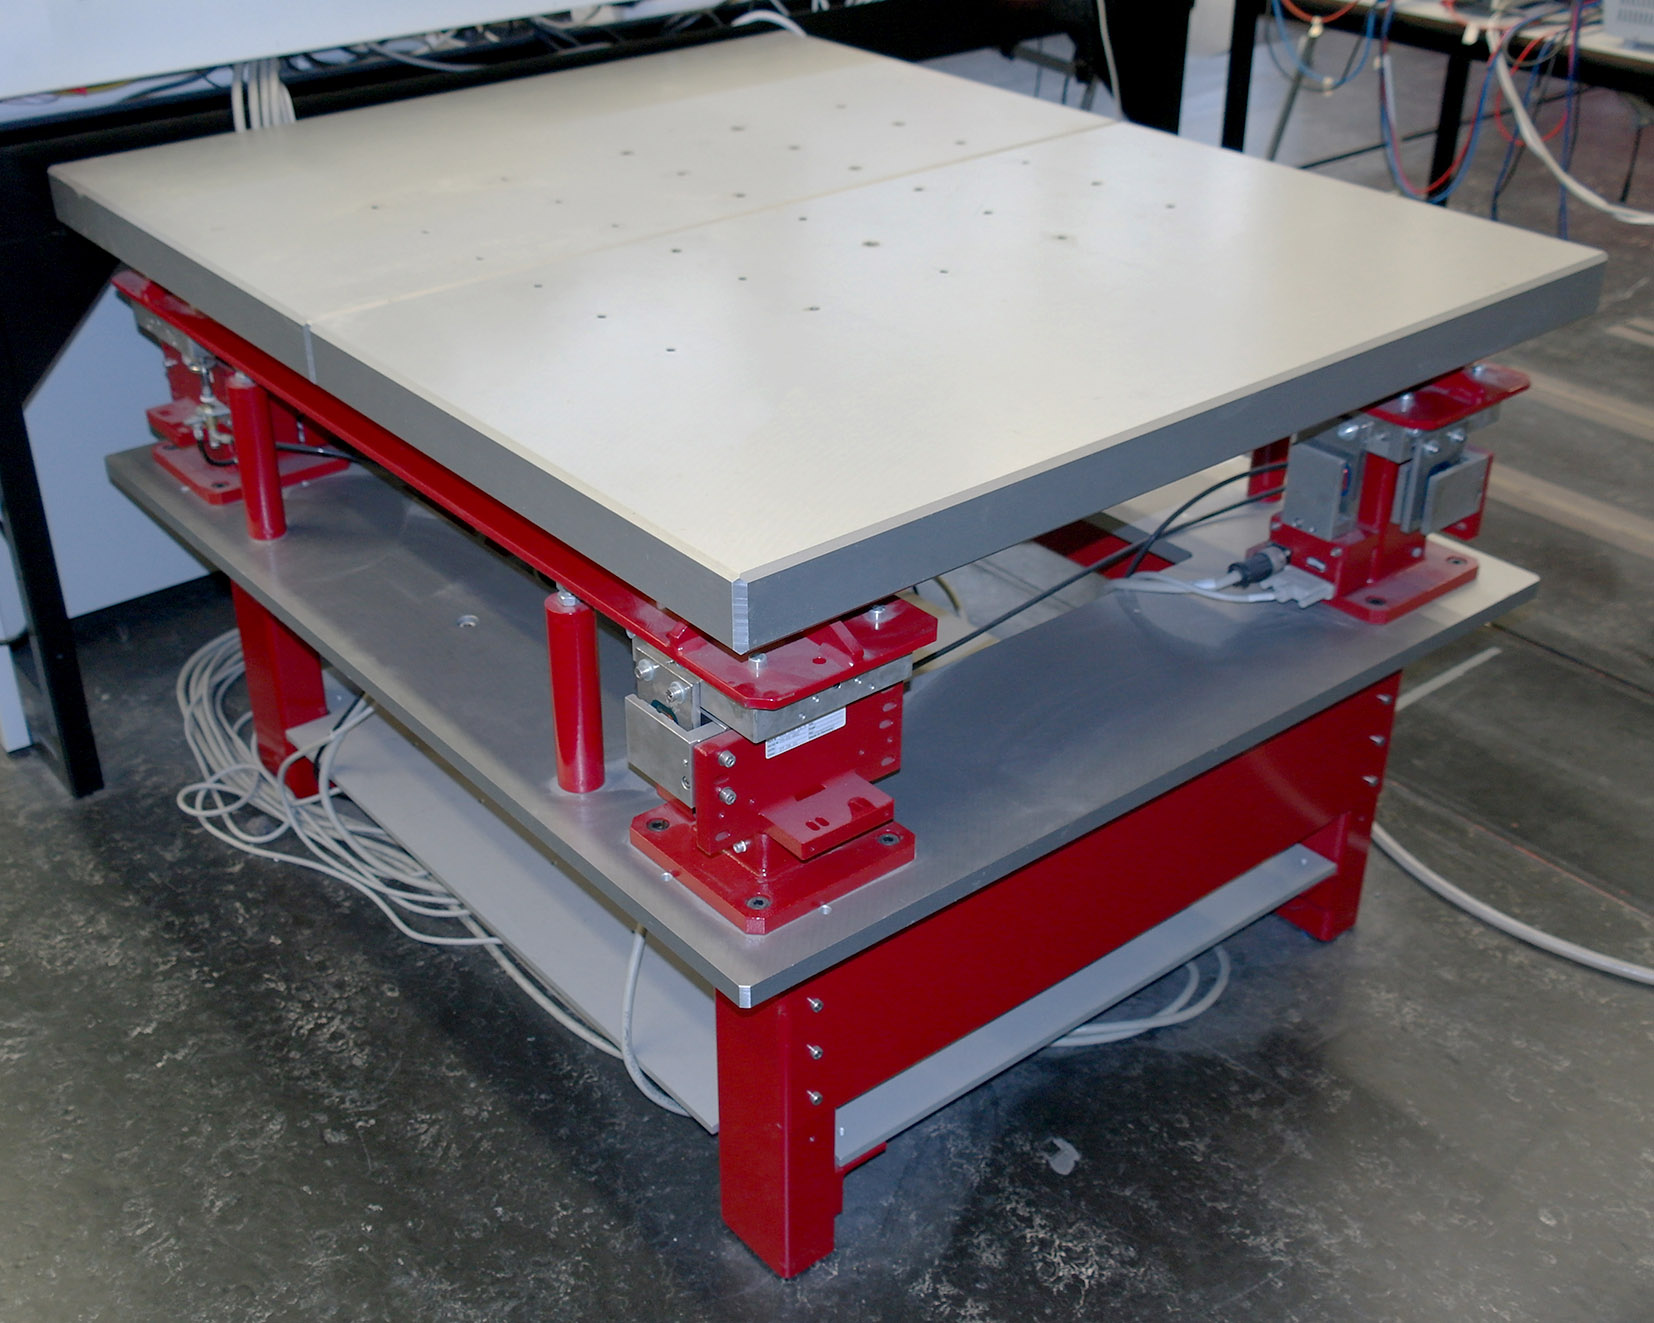
\includegraphics[width=\figurewidth]{\thisDir/figs/avis.jpg}}
  \caption{\Glsentryfirst{AVIS}.}
  \label{fig:lrmhinf:avis}
\end{figure}

\begin{figure}[p]
  \centering
  \setlength{\figurewidth}{0.475\columnwidth}
  \photobox{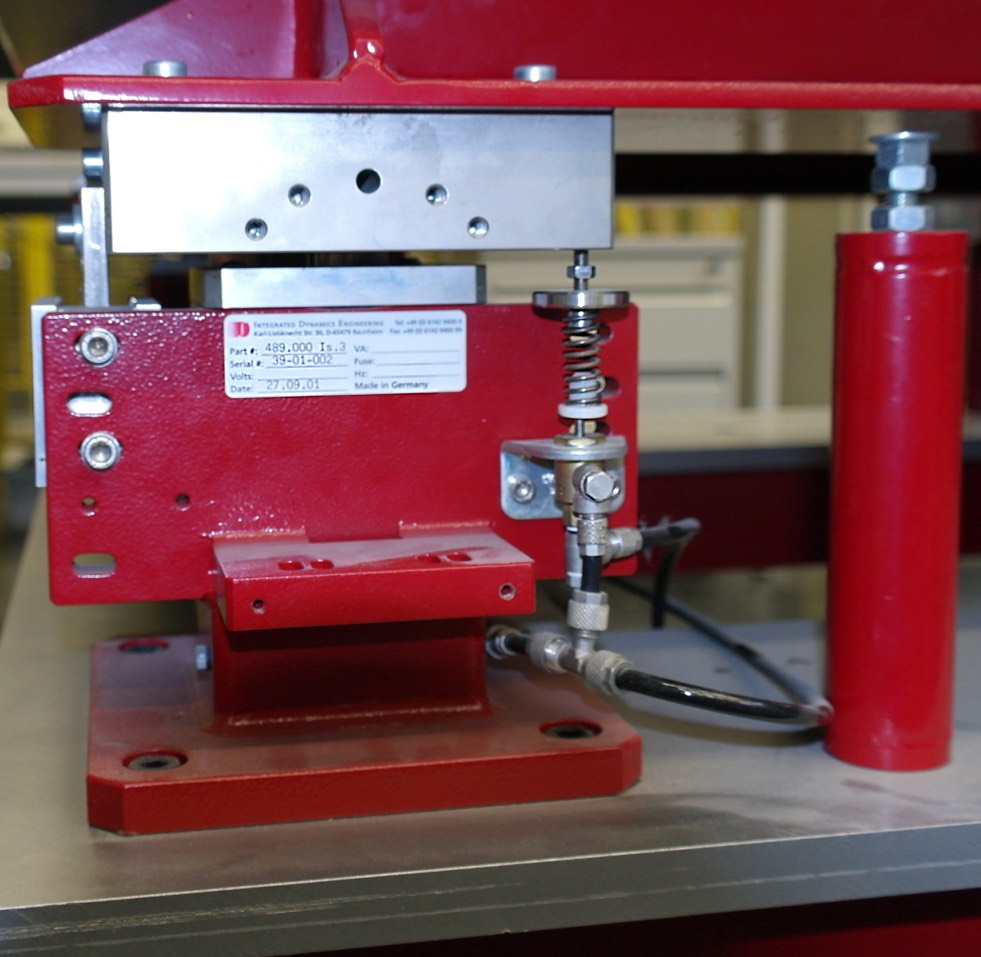
\includegraphics[width=\figurewidth]{\thisDir/figs/avis-airmount-cropped.jpg}}
  \hfill
  \photobox{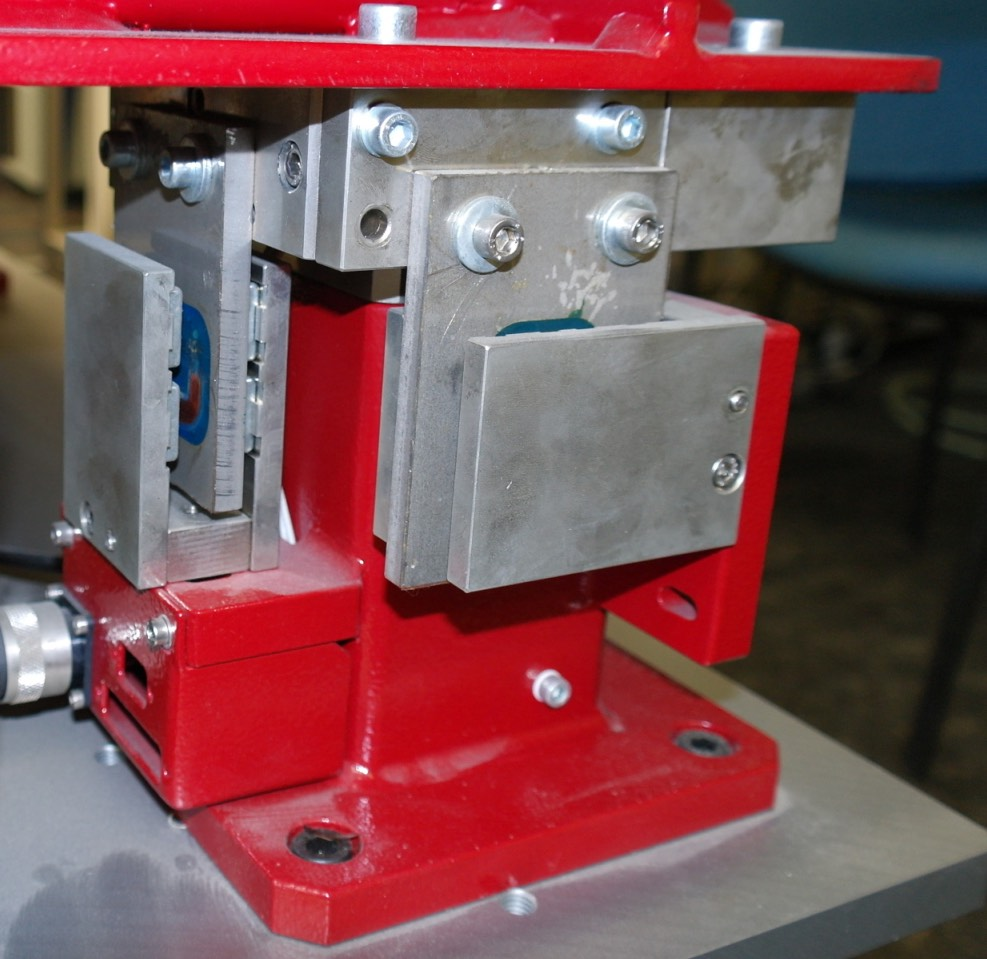
\includegraphics[width=1.005\figurewidth]{\thisDir/figs/avis-motors-cropped.jpg}}
  \caption[\glsentryshort{AVIS} isolation module.]{Isolation module of the \glsentrytext{AVIS}. 
  The left photo shows one of the air mounts providing passive vibration isolation.
  The right photo shows two linear motors that play a role in the active vibration isolation.}
  \label{fig:lrmhinf:avis:details}
\end{figure}

\subsection{Measurement \& Control Framework}
\label{sec:lrmhinf:control}
The experiments on the \gls{AVIS} are carried out in closed-loop (\figref{fig:lrmhinf:tpc}) with $r_2 = 0$.
The controller $\Controller=\experimental\Controller$ is a diagonal \gls{PI} regulator which stabilizes the \gls{AVIS} but yields only moderate vibration isolation.
See \appref{app:avis-setup} for detailed information regarding both the experimental setup and the experimental controller.
The $r_1$ input consists of five periods of a random phase multisine of $65\,536$ samples with excited bins such that $\omega_k \approx 1.001 \omega_{k-1}$  and $\Ts=1\unit{ms}$.
See \chapref{sec:excitation} and \citep{Geerardyn2013TIM} for more information regarding the design of such a signal.

\begin{figure}
 \centering
 \begin{tikzpicture}[scale=1,auto, >=stealth]
    \matrix[ampersand replacement=\&, row sep=0.3cm, column sep=0.6cm] {
%% FIRST ROW
        \node (r1) {$r_1$}; \&
        \&
        \&
        \&
        \node (guide) {}; \&
        \&
        \&
        \&
        \node        (uout) {$u$};  \\
%% SECOND ROW
        \node         (r2) {$r_2$}; \&
        \&
        \node[sum]    (sum2)  {};   \&
        \node[block]  (C)  {$C$};   \&
        \node[sum]    (sum1)  {};   \&
        \node[branch] (u)  {};      \&
        \node[block,color=modelset]  (P)  {$\ModelSet$};   \&
        \node[branch] (y)  {};      \&
        \node       (yout) {$y$};   \\
    };

    \draw [connector] (r2)   -- (sum2);
    \draw [connector] (sum2) -- node {$e_{\vphantom{c}}$}  (C);
    \draw [connector] (C)    -- node {$u_c$}  (sum1);
    \draw [connector] (sum1) -- (P);
    \draw [connector] (P)    -- (yout);
    \draw [connector] (r1)   -| (sum1);
    \draw [connector] (u)    |- (uout);
    \draw [connector] (y)    -- ++(0,-2em) -| node[near end,name=min] {\rotatebox{90}{$-$}} (sum2);

   \begin{pgfonlayer}{background}
     \node[groupbox=TPC, fit=(sum2) (y) (C) (min) (guide)] (TPC) {};
     \node at (TPC.north) [color=TPC, above] {$\ClosedLoop{\ModelSet[],\Controller}$};
   \end{pgfonlayer}

  \end{tikzpicture}

 \caption[Closed-loop block schematic.]{The considered feedback configuration $\ClosedLoop{\ModelSet[],\Controller}$.}
 \label{fig:lrmhinf:tpc}
\end{figure}

\begin{figure}
 \centering
 \begin{tikzpicture}[scale=1, >=stealth]
    \matrix[ampersand replacement=\&, row sep=0.2cm, column sep=0.32cm] {
%% FIRST ROW
        \node        (r1)   {$r_1$};              \&[-0.5em]
        \&
        \&
        \&
        \&
        \&
        \&
        \node[block] (NCp)   {$N_c$};              \&[-0.5em]
        \&[-0.5em]
        \node[block] (DCp)   {$D_c$};              \\
%% SECOND ROW
        \&
        \&
        \&
        \&
        \&
        \&
        \&
        \&
        \node[block] (Delta) {$\Delta$};          \\
%% THIRD ROW
        \node         (r2)   {$r_2$};             \&
        \&
        \node[sum]    (sum2) {};                  \&
        \node[block]  (DC)   {$D_c^{-1}$};        \&
        \node[block]  (NC)   {$N_c$};             \&
        \node[sum]    (sum1) {};                  \&
        \node[sum]    (u)    {};                  \&
        \node[block]  (DP)   {$\hat{D}^ {-1}$};   \&
        \&
        \node[block]  (NP)   {$\hat{N}$};         \&
        \node[sum]    (y)    {};                  \&
        \node         (yout) {$y$};               \\
    };

    \draw [connector] (r1)   -| (sum1);

    \draw [connector] (r2)   -- (sum2);
    \draw [connector] (sum2) -- (DC);
    \draw [connector] (DC)   -- (NC);
    \draw [connector] (NC)   -- (sum1);
    \draw [connector] (sum1) --  node[pos=0.3,above] {$u$} (u);
    \draw [connector] (u)    -- (DP);
    \draw [connector] (DP)   -- (NP);
    \draw [connector] (NP)   -- (y);
    
    \draw [connector] (y)    -- (yout);
    
    \draw [connector] (DP)    -| node [below,name=ud] {$u_{\Delta}$} (Delta);
    \draw [connector] (Delta) |- node [above,name=yd] {$y_{\Delta}$} (DCp) ;
    \draw [connector] (Delta) |- (NCp) ;
    \draw [connector] (DCp)   -| (y) ;
    \draw [connector] (NCp)   -| (u) ;

    \draw [connector] (y) -- ++(0.5em,0) -- ++(0,-2em) -| node[near end,left] {\rotatebox{90}{$-$}} (sum2);

    \begin{pgfonlayer}{background}

      \node[groupbox=controller,fit=(NC) (DC)]                            (C) {};
      \node[groupbox=plant,fit=(NP) (DP)]                           (P) {};
      \node[groupbox=plantset,fit=(P) (Delta) (DCp) (NCp) (y) (u)] (setP) {};

      \node at (C.north)      [color=controller, above]   {$C$};
      \node at (P.north west) [color=plant, above]  {$\hat{P}$};
      \node at (setP.north)   [color=plantset, above] {$\mathcal{P}$};

    \end{pgfonlayer}
\end{tikzpicture}

 \caption[Dual-Youla parametrization.]{Dual-Youla parametrization of the closed-loop set-up  with controller $\Controller$,  model set $\ModelSet[]$ and nominal plant model $\estimated\Plant$.}
\label{fig:lrmhinf:dualYoula}
\end{figure}

The parametrization of the plant model set $\ModelSet[]$ conforms to the dual-\YK{} framework~\citep{Hansen1989,Anderson1998} that parametrizes $\ModelSet[]$ in terms of  all plants $P$ that are stabilized by the controller $C$:
\begin{equation}
  \ModelSet[] 
    \isdef 
      \Set{
            \frac{\hat{N} + D_c \Delta}
                 {\hat{D} - N_c \Delta} 
          |
            \infnorm{\Delta} \leq \gamma
        }
  \label{eq:lrmhinf:dualYoulaModelSet}
  \text{,}
\end{equation}
where $C=N_c D_c^{-1}$ and $\estimated\Plant = \estimated{N}\estimated{D}^{-1}$ are decomposed as \gls{RCF} (see \figref{fig:lrmhinf:dualYoula}).
To estimate $\Delta$ and $\infnorm{\Delta}$, the signals $u_{\Delta}$ and $y_{\Delta}$ in~\figref{fig:lrmhinf:dualYoula} are required.
These can be computed from $u$ and $y$ directly~\citep{Anderson1998}:
\begin{align}
  u_{\Delta}(t) &= \left(\hat{D} + C \hat{N} \right)^{-1} \mat{C & \I} \mat{y(t)\\u(t)}\\
  y_{\Delta}(t) &= \left(D_c + \hat{P} N_c \right)^{-1} \mat{\I & -\hat{P}} \mat{y(t)\\u(t)}
\end{align}
In addition, $u_{\Delta}$ is noise free under standard assumptions~\citep{Hansen1989} and uncorrelated to $y_{\Delta}$. 
Hence the method of \secref{sec:lrmhinf:LPMHinf} applies directly.

The non-uniqueness of the \gls{RCF} can be exploited to satisfy additional conditions.
In view of the robust control criterion
\begin{equation}
  \Crit(\Plant,\Controller) 
    \isdef 
      \infnorm{W \ClosedLoop{\Plant,\Controller} V}
  \label{eq:lrmhinf:controlCrit}
  \text{,}
\end{equation}
the \glspl{RCF} are constructed such that
$
  \worstCase\Crit \left( \ModelSet[], \experimental\Controller \right)
  \leq
  \Crit \left( \estimated\Plant, \experimental\Controller \right)
  + \gamma
$
where $\worstCase\Crit(\ModelSet[],C) \isdef \sup_{P\in\ModelSet[]} \Crit(P,C)$~\citep{Oomen2012SIRP}.
% Obviously, $\Crit( \true\Plant, \experimental\Controller) \leq \worstCase\Crit ( \ModelSet[], \experimental\Controller )$ is guaranteed when $\true\Plant \in \ModelSet[]$.
I.e. even for a weighted control criterion \eqref{eq:lrmhinf:controlCrit}, there is no need to incorporate weights $W'$ and $V'$ into the estimation of the uncertainty bound as $\infnorm{W' \Delta V'}$.
In this chapter, an eighth-order $\estimated\Plant$~(\figref{fig:lrmhinf:avis-frf}) is estimated.
Some dynamics are left unmodeled and are hence part of $\Delta$~(\figref{fig:lrmhinf:avisMeas}).

\begin{figure}
 \centering
    \setlength{\figurewidth}{0.75\columnwidth}
    \setlength{\figureheight}{0.68\figurewidth}
    % This file was created by matlab2tikz v0.4.3 (commit 2110609f2d993ab5074ce6b8f3e699d75d77a6b6).
% Copyright (c) 2008--2013, Nico Schlömer <nico.schloemer@gmail.com>
% All rights reserved.
% 
% The latest updates can be retrieved from
%   http://www.mathworks.com/matlabcentral/fileexchange/22022-matlab2tikz
% where you can also make suggestions and rate matlab2tikz.
% 
\begin{tikzpicture}

\begin{axis}[%
width=\figurewidth,
height=\figureheight,
scale only axis,
xmode=log,
xmin=9.9,
xmax=500,
ymajorgrids,
xmajorgrids,
xminorgrids,
xminorticks=true,
ymin=-70,
ymax=16,
ylabel={Amplitude $\abs{P}$ \axisunit{dB}},
xlabel={Frequency $\omega$  \axisunit{Hz}},
name=plot0
]

\addplot [paramPhat]
table[row sep=crcr] {
% 0.0152587890625 23.7722447525977\\
% 0.0457763671875 22.3080847897672\\
% 0.0762939453125 20.2741569707957\\
% 0.1068115234375 18.2257529897462\\
% 0.1373291015625 16.3079974146639\\
% 0.1678466796875 14.5181085972517\\
% 0.1983642578125 12.8172522087776\\
% 0.2288818359375 11.1608733787134\\
% 0.2593994140625 9.50397723607956\\
% 0.2899169921875 7.79899510770321\\
% 0.3204345703125 5.99029715556577\\
% 0.3509521484375 4.00469298301403\\
% 0.3814697265625 1.73365389099158\\
% 0.4119873046875 -1.00426577865468\\
% 0.4425048828125 -4.54966533123516\\
% 0.4730224609375 -9.51643537709583\\
% 0.5035400390625 -13.8964915122691\\
% 0.5340576171875 -9.50421779076407\\
% 0.5645751953125 -5.12612382304163\\
% 0.5950927734375 -2.12859036094432\\
% 0.6256103515625 0.0795243024252674\\
% 0.6561279296875 1.81283230611915\\
% 0.6866455078125 3.23551080308591\\
% 0.7171630859375 4.44140167314812\\
% 0.7476806640625 5.48852713143906\\
% 0.7781982421875 6.41503322856487\\
% 0.8087158203125 7.24723490797363\\
% 0.8392333984375 8.00399673011526\\
% 0.8697509765625 8.69927256044658\\
% 0.9002685546875 9.34365587383497\\
% 0.9307861328125 9.94536758467433\\
% 0.9613037109375 10.5109086205\\
% 0.9918212890625 11.0455044893486\\
% 1.0223388671875 11.5534162767064\\
% 1.0528564453125 12.0381632797992\\
% 1.0833740234375 12.5026856473201\\
% 1.1138916015625 12.9494653430929\\
% 1.1444091796875 13.3806175660085\\
% 1.1749267578125 13.7979608445429\\
% 1.2054443359375 14.2030714862825\\
% 1.2359619140625 14.5973263807037\\
% 1.2664794921875 14.9819370161158\\
% 1.2969970703125 15.3579767887555\\
% 1.3275146484375 15.7264031341724\\
% 1.3580322265625 16.0880756219148\\
% 1.3885498046875 16.4437708743058\\
% 1.4190673828125 16.7941949657516\\
% 1.4495849609375 17.1399938082556\\
% 1.4801025390625 17.4817619163763\\
% 1.5106201171875 17.8200498601774\\
% 1.5411376953125 18.1553706503383\\
% 1.5716552734375 18.4882052502356\\
% 1.6021728515625 18.8190073716575\\
% 1.6326904296875 19.1482076811222\\
% 1.6632080078125 19.4762175204909\\
% 1.6937255859375 19.8034322272109\\
% 1.7242431640625 20.1302341249468\\
% 1.7547607421875 20.4569952437229\\
% 1.7852783203125 20.7840798193475\\
% 1.8157958984375 21.1118466143154\\
% 1.8463134765625 21.4406510961916\\
% 1.8768310546875 21.7708475043434\\
% 1.9073486328125 22.1027908315403\\
% 1.9378662109375 22.4368387431394\\
% 1.9683837890625 22.7733534531064\\
% 1.9989013671875 23.112703572744\\
% 2.0294189453125 23.4552659444922\\
% 2.0599365234375 23.8014274692076\\
% 2.0904541015625 24.1515869305938\\
% 2.1209716796875 24.5061568144554\\
% 2.1514892578125 24.8655651125802\\
% 2.1820068359375 25.2302570904768\\
% 2.2125244140625 25.600696983754\\
% 2.2430419921875 25.9773695680442\\
% 2.2735595703125 26.3607815198056\\
% 2.3040771484375 26.7514624470049\\
% 2.3345947265625 27.1499654151986\\
% 2.3651123046875 27.556866719776\\
% 2.3956298828125 27.9727645504501\\
% 2.4261474609375 28.398276047329\\
% 2.4566650390625 28.8340320419987\\
% 2.4871826171875 29.2806684882203\\
% 2.5177001953125 29.738813182202\\
% 2.5482177734375 30.2090658074338\\
% 2.5787353515625 30.6919685550836\\
% 2.6092529296875 31.1879634947029\\
% 2.6397705078125 31.6973314186676\\
% 2.6702880859375 32.2201049841374\\
% 2.7008056640625 32.7559466142805\\
% 2.7313232421875 33.3039789538858\\
% 2.7618408203125 33.8625532646832\\
% 2.7923583984375 34.4289403934151\\
% 2.8228759765625 34.998932818317\\
% 2.8533935546875 35.5663602956612\\
% 2.8839111328125 36.1225545670644\\
% 2.9144287109375 36.6558610950166\\
% 2.9449462890625 37.1513927585097\\
% 2.9754638671875 37.5913317342492\\
% 3.0059814453125 37.9561374983115\\
% 3.0364990234375 38.2268760492636\\
% 3.0670166015625 38.388435532638\\
% 3.0975341796875 38.4327465267617\\
% 3.1280517578125 38.3607353513796\\
% 3.1585693359375 38.1820974821149\\
% 3.1890869140625 37.9130018010624\\
% 3.2196044921875 37.5727752169157\\
% 3.2501220703125 37.1808111366764\\
% 3.2806396484375 36.7544592218602\\
% 3.3111572265625 36.3080196085472\\
% 3.3416748046875 35.8525763470607\\
% 3.3721923828125 35.3963117506141\\
% 3.4027099609375 34.9450157498753\\
% 3.4332275390625 34.5026165737593\\
% 3.4637451171875 34.0716497331852\\
% 3.4942626953125 33.6536382712904\\
% 3.5247802734375 33.249385659551\\
% 3.5552978515625 32.8591941702117\\
% 3.5858154296875 32.4830241866703\\
% 3.6163330078125 32.1206086666063\\
% 3.6468505859375 31.771534437305\\
% 3.6773681640625 31.4352993686595\\
% 3.7078857421875 31.1113521929172\\
% 3.7384033203125 30.7991199322042\\
% 3.7689208984375 30.4980265233318\\
% 3.7994384765625 30.2075052166461\\
% 3.8299560546875 29.9270065898856\\
% 3.8604736328125 29.6560034886193\\
% 3.8909912109375 29.3939938260787\\
% 3.9215087890625 29.1405019050057\\
% 3.9520263671875 28.8950787316553\\
% 3.9825439453125 28.6573016549751\\
% 4.0130615234375 28.4267735662919\\
% 4.0435791015625 28.2031218251764\\
% 4.0740966796875 27.9859970274679\\
% 4.1046142578125 27.775071695985\\
% 4.1351318359375 27.5700389491584\\
% 4.1656494140625 27.3706111848061\\
% 4.1961669921875 27.1765188034565\\
% 4.2266845703125 26.9875089865579\\
% 4.2572021484375 26.8033445385226\\
% 4.2877197265625 26.6238027970888\\
% 4.3182373046875 26.448674613411\\
% 4.3487548828125 26.2777634012001\\
% 4.3792724609375 26.1108842528586\\
% 4.4097900390625 25.9478631196883\\
% 4.4403076171875 25.7885360527342\\
% 4.4708251953125 25.6327485005659\\
% 4.5013427734375 25.4803546602147\\
% 4.5318603515625 25.3312168775128\\
% 4.5623779296875 25.1852050931961\\
% 4.5928955078125 25.0421963312868\\
% 4.6234130859375 24.9020742264696\\
% 4.6539306640625 24.7647285873746\\
% 4.6844482421875 24.6300549928949\\
% 4.7149658203125 24.4979544188742\\
% 4.7454833984375 24.3683328927045\\
% 4.7760009765625 24.2411011735653\\
% 4.8065185546875 24.1161744562232\\
% 4.8370361328125 23.9934720964781\\
% 4.8675537109375 23.8729173565049\\
% 4.8980712890625 23.7544371684859\\
% 4.9285888671875 23.6379619150655\\
% 4.9591064453125 23.5234252252845\\
% 4.9896240234375 23.4107637847641\\
% 5.0201416015625 23.2999171590175\\
% 5.0506591796875 23.1908276288606\\
% 5.0811767578125 23.0834400369808\\
% 5.1116943359375 22.9777016448047\\
% 5.1422119140625 22.8735619988752\\
% 5.1727294921875 22.7709728060182\\
% 5.2032470703125 22.6698878166361\\
% 5.2337646484375 22.5702627155228\\
% 5.2642822265625 22.4720550196442\\
% 5.2947998046875 22.3752239823726\\
% 5.3253173828125 22.2797305037082\\
% 5.3558349609375 22.1855370460544\\
% 5.3863525390625 22.0926075551535\\
% 5.4168701171875 22.0009073858157\\
% 5.4473876953125 21.9104032321067\\
% 5.4779052734375 21.8210630616861\\
% 5.5084228515625 21.7328560540075\\
% 5.5389404296875 21.6457525421218\\
% 5.5694580078125 21.5597239578368\\
% 5.5999755859375 21.4747427800109\\
% 5.6304931640625 21.3907824857722\\
% 5.6610107421875 21.3078175044717\\
% 5.6915283203125 21.2258231741913\\
% 5.7220458984375 21.1447757006444\\
% 5.7525634765625 21.0646521183131\\
% 5.7830810546875 20.9854302536835\\
% 5.8135986328125 20.9070886904451\\
% 5.8441162109375 20.8296067365336\\
% 5.8746337890625 20.7529643929023\\
% 5.9051513671875 20.6771423239184\\
% 5.9356689453125 20.6021218292832\\
% 5.9661865234375 20.5278848173871\\
% 5.9967041015625 20.4544137800129\\
% 6.0272216796875 20.3816917683075\\
% 6.0577392578125 20.3097023699493\\
% 6.0882568359375 20.2384296874399\\
% 6.1187744140625 20.1678583174577\\
% 6.1492919921875 20.0979733312107\\
% 6.1798095703125 20.0287602557339\\
% 6.2103271484375 19.9602050560772\\
% 6.2408447265625 19.8922941183343\\
% 6.2713623046875 19.8250142334668\\
% 6.3018798828125 19.7583525818799\\
% 6.3323974609375 19.6922967187082\\
% 6.3629150390625 19.6268345597746\\
% 6.3934326171875 19.5619543681849\\
% 6.4239501953125 19.4976447415258\\
% 6.4544677734375 19.4338945996339\\
% 6.4849853515625 19.370693172906\\
% 6.5155029296875 19.3080299911225\\
% 6.5460205078125 19.2458948727579\\
% 6.5765380859375 19.1842779147538\\
% 6.6070556640625 19.1231694827303\\
% 6.6375732421875 19.0625602016145\\
% 6.6680908203125 19.0024409466643\\
% 6.6986083984375 18.9428028348697\\
% 6.7291259765625 18.8836372167118\\
% 6.7596435546875 18.8249356682611\\
% 6.7901611328125 18.7666899836022\\
% 6.8206787109375 18.7088921675647\\
% 6.8511962890625 18.6515344287496\\
% 6.8817138671875 18.5946091728347\\
% 6.9122314453125 18.5381089961471\\
% 6.9427490234375 18.4820266794898\\
% 6.9732666015625 18.4263551822117\\
% 7.0037841796875 18.3710876365075\\
% 7.0343017578125 18.3162173419396\\
% 7.0648193359375 18.2617377601706\\
% 7.0953369140625 18.2076425098967\\
% 7.1258544921875 18.1539253619737\\
% 7.1563720703125 18.1005802347269\\
% 7.1868896484375 18.0476011894361\\
% 7.2174072265625 17.9949824259891\\
% 7.2479248046875 17.9427182786955\\
% 7.2784423828125 17.8908032122542\\
% 7.3089599609375 17.8392318178679\\
% 7.3394775390625 17.7879988094988\\
% 7.3699951171875 17.7370990202583\\
% 7.4005126953125 17.6865273989263\\
% 7.4310302734375 17.6362790065947\\
% 7.4615478515625 17.5863490134282\\
% 7.4920654296875 17.5367326955395\\
% 7.5225830078125 17.487425431974\\
% 7.5531005859375 17.4384227017976\\
% 7.5836181640625 17.389720081286\\
% 7.6141357421875 17.3413132412099\\
% 7.6446533203125 17.2931979442118\\
% 7.6751708984375 17.2453700422729\\
% 7.7056884765625 17.1978254742634\\
% 7.7362060546875 17.1505602635765\\
% 7.7667236328125 17.1035705158395\\
% 7.7972412109375 17.0568524167007\\
% 7.8277587890625 17.0104022296899\\
% 7.8582763671875 16.9642162941472\\
% 7.8887939453125 16.9182910232204\\
% 7.9193115234375 16.8726229019257\\
% 7.9498291015625 16.8272084852716\\
% 7.9803466796875 16.7820443964416\\
% 8.0108642578125 16.7371273250358\\
% 8.0413818359375 16.6924540253663\\
% 8.0718994140625 16.6480213148072\\
% 8.1024169921875 16.6038260721958\\
% 8.1329345703125 16.5598652362826\\
% 8.1634521484375 16.5161358042302\\
% 8.1939697265625 16.472634830157\\
% 8.2244873046875 16.4293594237263\\
% 8.2550048828125 16.3863067487773\\
% 8.2855224609375 16.3434740219981\\
% 8.3160400390625 16.3008585116377\\
% 8.3465576171875 16.2584575362571\\
% 8.3770751953125 16.2162684635168\\
% 8.4075927734375 16.1742887090009\\
% 8.4381103515625 16.1325157350745\\
% 8.4686279296875 16.0909470497756\\
% 8.4991455078125 16.0495802057382\\
% 8.5296630859375 16.0084127991474\\
% 8.5601806640625 15.9674424687237\\
% 8.5906982421875 15.9266668947367\\
% 8.6212158203125 15.8860837980471\\
% 8.6517333984375 15.8456909391749\\
% 8.6822509765625 15.8054861173949\\
% 8.7127685546875 15.7654671698568\\
% 8.7432861328125 15.72563197073\\
% 8.7738037109375 15.685978430372\\
% 8.8043212890625 15.6465044945199\\
% 8.8348388671875 15.6072081435041\\
% 8.8653564453125 15.5680873914829\\
% 8.8958740234375 15.529140285699\\
% 8.9263916015625 15.4903649057547\\
% 8.9569091796875 15.4517593629078\\
% 8.9874267578125 15.4133217993855\\
% 9.0179443359375 15.3750503877171\\
% 9.0484619140625 15.3369433300839\\
% 9.0789794921875 15.298998857687\\
% 9.1094970703125 15.2612152301306\\
% 9.1400146484375 15.2235907348225\\
% 9.1705322265625 15.1861236863892\\
% 9.2010498046875 15.1488124261069\\
% 9.2315673828125 15.111655321347\\
% 9.2620849609375 15.0746507650352\\
% 9.2926025390625 15.0377971751251\\
% 9.3231201171875 15.001092994085\\
% 9.3536376953125 14.9645366883972\\
% 9.3841552734375 14.9281267480708\\
% 9.4146728515625 14.8918616861655\\
% 9.4451904296875 14.8557400383283\\
% 9.4757080078125 14.8197603623414\\
% 9.5062255859375 14.7839212376807\\
% 9.5367431640625 14.748221265086\\
% 9.5672607421875 14.7126590661409\\
% 9.5977783203125 14.677233282864\\
% 9.6282958984375 14.6419425773086\\
% 9.6588134765625 14.6067856311732\\
% 9.6893310546875 14.5717611454208\\
% 9.7198486328125 14.5368678399078\\
% 9.7503662109375 14.5021044530208\\
9.7808837890625 14.4674697413231\\
9.8114013671875 14.4329624792088\\
9.8419189453125 14.3985814585653\\
9.8724365234375 14.3643254884439\\
9.9029541015625 14.3301933947372\\
9.9334716796875 14.2961840198655\\
9.9639892578125 14.2622962224688\\
9.9945068359375 14.228528877107\\
10.0250244140625 14.1948808739665\\
10.0555419921875 14.1613511185736\\
10.0860595703125 14.1279385315143\\
10.1165771484375 14.0946420481607\\
10.1470947265625 14.0614606184031\\
10.1776123046875 14.0283932063886\\
10.2081298828125 13.9954387902654\\
10.2386474609375 13.9625963619322\\
10.2691650390625 13.9298649267941\\
10.2996826171875 13.8972435035233\\
10.3302001953125 13.8647311238251\\
10.3607177734375 13.8323268322089\\
10.3912353515625 13.8000296857646\\
10.4217529296875 13.7678387539438\\
10.4522705078125 13.7357531183448\\
10.4827880859375 13.7037718725037\\
10.5133056640625 13.6718941216888\\
10.5438232421875 13.6401189826999\\
10.5743408203125 13.6084455836716\\
10.6048583984375 13.5768730638813\\
10.6353759765625 13.5454005735605\\
10.6658935546875 13.5140272737106\\
10.6964111328125 13.4827523359222\\
10.7269287109375 13.4515749421985\\
10.7574462890625 13.4204942847822\\
10.7879638671875 13.3895095659856\\
10.8184814453125 13.3586199980252\\
10.8489990234375 13.3278248028585\\
10.8795166015625 13.2971232120247\\
10.9100341796875 13.266514466489\\
10.9405517578125 13.2359978164894\\
10.9710693359375 13.2055725213867\\
11.0015869140625 13.175237849518\\
11.0321044921875 13.1449930780526\\
11.0626220703125 13.1148374928508\\
11.0931396484375 13.0847703883262\\
11.1236572265625 13.0547910673096\\
11.1541748046875 13.0248988409165\\
11.1846923828125 12.9950930284171\\
11.2152099609375 12.9653729571079\\
11.2457275390625 12.9357379621872\\
11.2762451171875 12.9061873866321\\
11.3067626953125 12.876720581078\\
11.3372802734375 12.847336903701\\
11.3677978515625 12.8180357201012\\
11.3983154296875 12.7888164031902\\
11.4288330078125 12.7596783330788\\
11.4593505859375 12.7306208969682\\
11.4898681640625 12.7016434890426\\
11.5203857421875 12.6727455103641\\
11.5509033203125 12.643926368769\\
11.5814208984375 12.6151854787671\\
11.6119384765625 12.5865222614421\\
11.6424560546875 12.5579361443536\\
11.6729736328125 12.529426561442\\
11.7034912109375 12.5009929529339\\
11.7340087890625 12.4726347652501\\
11.7645263671875 12.444351450915\\
11.7950439453125 12.4161424684678\\
11.8255615234375 12.3880072823747\\
11.8560791015625 12.3599453629436\\
11.8865966796875 12.3319561862398\\
11.9171142578125 12.3040392340031\\
11.9476318359375 12.276193993567\\
11.9781494140625 12.2484199577786\\
12.0086669921875 12.2207166249204\\
12.0391845703125 12.1930834986332\\
12.0697021484375 12.1655200878409\\
12.1002197265625 12.1380259066756\\
12.1307373046875 12.1106004744055\\
12.1612548828125 12.0832433153624\\
12.1917724609375 12.0559539588717\\
12.2222900390625 12.0287319391832\\
12.2528076171875 12.0015767954029\\
12.2833251953125 11.9744880714262\\
12.3138427734375 11.9474653158724\\
12.3443603515625 11.92050808202\\
12.3748779296875 11.8936159277431\\
12.4053955078125 11.8667884154491\\
12.4359130859375 11.8400251120177\\
12.4664306640625 11.8133255887401\\
12.4969482421875 11.7866894212599\\
12.5274658203125 11.7601161895151\\
12.5579833984375 11.7336054776803\\
12.5885009765625 11.7071568741107\\
12.6190185546875 11.6807699712867\\
12.6495361328125 11.6544443657591\\
12.6800537109375 11.6281796580957\\
12.7105712890625 11.6019754528288\\
12.7410888671875 11.5758313584027\\
12.7716064453125 11.5497469871235\\
12.8021240234375 11.5237219551083\\
12.8326416015625 11.4977558822361\\
12.8631591796875 11.4718483920992\\
12.8936767578125 11.4459991119555\\
12.9241943359375 11.4202076726812\\
12.9547119140625 11.3944737087249\\
12.9852294921875 11.368796858062\\
13.0157470703125 11.3431767621495\\
13.0462646484375 11.3176130658826\\
13.0767822265625 11.2921054175508\\
13.1072998046875 11.2666534687952\\
13.1378173828125 11.241256874567\\
13.1683349609375 11.2159152930852\\
13.1988525390625 11.190628385797\\
13.2293701171875 11.1653958173365\\
13.2598876953125 11.1402172554864\\
13.2904052734375 11.1150923711383\\
13.3209228515625 11.0900208382547\\
13.3514404296875 11.0650023338314\\
13.3819580078125 11.0400365378604\\
13.4124755859375 11.0151231332933\\
13.4429931640625 10.9902618060052\\
13.4735107421875 10.9654522447596\\
13.5040283203125 10.9406941411732\\
13.5345458984375 10.9159871896818\\
13.5650634765625 10.8913310875061\\
13.5955810546875 10.8667255346189\\
13.6260986328125 10.8421702337115\\
13.6566162109375 10.8176648901621\\
13.6871337890625 10.7932092120036\\
13.7176513671875 10.768802909892\\
13.7481689453125 10.7444456970759\\
13.7786865234375 10.7201372893656\\
13.8092041015625 10.6958774051034\\
13.8397216796875 10.6716657651338\\
13.8702392578125 10.6475020927743\\
13.9007568359375 10.6233861137871\\
13.9312744140625 10.5993175563502\\
13.9617919921875 10.5752961510297\\
13.9923095703125 10.5513216307524\\
14.0228271484375 10.5273937307787\\
14.0533447265625 10.5035121886758\\
14.0838623046875 10.4796767442912\\
14.1143798828125 10.455887139727\\
14.1448974609375 10.4321431193141\\
14.1754150390625 10.4084444295873\\
14.2059326171875 10.3847908192599\\
14.2364501953125 10.3611820391997\\
14.2669677734375 10.3376178424043\\
14.2974853515625 10.3140979839777\\
14.3280029296875 10.2906222211067\\
14.3585205078125 10.2671903130375\\
14.3890380859375 10.2438020210529\\
14.4195556640625 10.22045710845\\
14.4500732421875 10.1971553405177\\
14.4805908203125 10.1738964845149\\
14.5111083984375 10.1506803096488\\
14.5416259765625 10.1275065870537\\
14.5721435546875 10.1043750897697\\
14.6026611328125 10.0812855927223\\
14.6331787109375 10.0582378727017\\
14.6636962890625 10.0352317083424\\
14.6942138671875 10.012266880104\\
14.7247314453125 9.98934317025066\\
14.7552490234375 9.96646036283231\\
14.7857666015625 9.9436182436653\\
14.8162841796875 9.92081660031357\\
14.8468017578125 9.89805522207\\
14.8773193359375 9.87533389993805\\
14.9078369140625 9.85265242661365\\
14.9383544921875 9.83001059646725\\
14.9688720703125 9.80740820552622\\
14.9993896484375 9.78484505145737\\
15.0299072265625 9.7623209335498\\
15.0604248046875 9.73983565269793\\
15.0909423828125 9.71738901138468\\
15.1214599609375 9.69498081366498\\
15.1519775390625 9.6726108651495\\
15.1824951171875 9.65027897298842\\
15.2130126953125 9.62798494585566\\
15.2435302734375 9.60572859393307\\
15.2740478515625 9.583509728895\\
15.3045654296875 9.561328163893\\
15.3350830078125 9.53918371354067\\
15.3656005859375 9.5170761938988\\
15.3961181640625 9.49500542246062\\
15.4266357421875 9.47297121813725\\
15.4571533203125 9.45097340124339\\
15.4876708984375 9.42901179348313\\
15.5181884765625 9.40708621793591\\
15.5487060546875 9.38519649904277\\
15.5792236328125 9.36334246259269\\
15.6097412109375 9.34152393570905\\
15.6402587890625 9.31974074683639\\
15.6707763671875 9.29799272572725\\
15.7012939453125 9.27627970342915\\
15.7318115234375 9.25460151227182\\
15.7623291015625 9.23295798585454\\
15.7928466796875 9.21134895903353\\
15.8233642578125 9.1897742679097\\
15.8538818359375 9.16823374981642\\
15.8843994140625 9.14672724330747\\
15.9149169921875 9.12525458814505\\
15.9454345703125 9.10381562528812\\
15.9759521484375 9.08241019688072\\
16.0064697265625 9.0610381462405\\
16.0369873046875 9.03969931784732\\
16.0675048828125 9.01839355733217\\
16.0980224609375 8.99712071146595\\
16.1285400390625 8.97588062814859\\
16.1590576171875 8.95467315639825\\
16.1895751953125 8.9334981463406\\
16.2200927734375 8.91235544919827\\
16.2506103515625 8.89124491728043\\
16.2811279296875 8.87016640397246\\
16.3116455078125 8.84911976372578\\
16.3421630859375 8.82810485204775\\
16.3726806640625 8.80712152549171\\
16.4031982421875 8.78616964164721\\
16.4337158203125 8.76524905913021\\
16.4642333984375 8.7443596375735\\
16.4947509765625 8.72350123761718\\
16.5252685546875 8.70267372089935\\
16.5557861328125 8.68187695004671\\
16.5863037109375 8.66111078866546\\
16.6168212890625 8.64037510133222\\
16.6473388671875 8.61966975358509\\
16.6778564453125 8.59899461191467\\
16.7083740234375 8.57834954375548\\
16.7388916015625 8.55773441747715\\
16.7694091796875 8.53714910237591\\
16.7999267578125 8.51659346866614\\
16.8304443359375 8.49606738747194\\
16.8609619140625 8.4755707308189\\
16.8914794921875 8.45510337162595\\
16.9219970703125 8.43466518369715\\
16.9525146484375 8.41425604171381\\
16.9830322265625 8.39387582122649\\
17.0135498046875 8.37352439864721\\
17.0440673828125 8.35320165124173\\
17.0745849609375 8.33290745712187\\
17.1051025390625 8.31264169523793\\
17.1356201171875 8.29240424537123\\
17.1661376953125 8.27219498812669\\
17.1966552734375 8.25201380492555\\
17.2271728515625 8.23186057799806\\
17.2576904296875 8.21173519037637\\
17.2882080078125 8.19163752588742\\
17.3187255859375 8.17156746914593\\
17.3492431640625 8.15152490554753\\
17.3797607421875 8.13150972126179\\
17.4102783203125 8.11152180322553\\
17.4407958984375 8.09156103913611\\
17.4713134765625 8.07162731744471\\
17.5018310546875 8.05172052734986\\
17.5323486328125 8.03184055879088\\
17.5628662109375 8.0119873024415\\
17.5933837890625 7.99216064970347\\
17.6239013671875 7.97236049270026\\
17.6544189453125 7.95258672427089\\
17.6849365234375 7.93283923796372\\
17.7154541015625 7.91311792803038\\
17.7459716796875 7.89342268941975\\
17.7764892578125 7.87375341777194\\
17.8070068359375 7.8541100094125\\
17.8375244140625 7.83449236134646\\
17.8680419921875 7.81490037125262\\
17.8985595703125 7.79533393747781\\
17.9290771484375 7.77579295903122\\
17.9595947265625 7.75627733557886\\
17.9901123046875 7.73678696743791\\
18.0206298828125 7.71732175557132\\
18.0511474609375 7.69788160158236\\
18.0816650390625 7.67846640770924\\
18.1121826171875 7.6590760768198\\
18.1427001953125 7.63971051240622\\
18.1732177734375 7.62036961857987\\
18.2037353515625 7.60105330006607\\
18.2342529296875 7.58176146219908\\
18.2647705078125 7.56249401091696\\
18.2952880859375 7.54325085275665\\
18.3258056640625 7.52403189484894\\
18.3563232421875 7.50483704491362\\
18.3868408203125 7.48566621125467\\
18.4173583984375 7.46651930275532\\
18.4478759765625 7.44739622887348\\
18.4783935546875 7.42829689963687\\
18.5089111328125 7.40922122563846\\
18.5394287109375 7.39016911803183\\
18.5699462890625 7.37114048852659\\
18.6004638671875 7.3521352493839\\
18.6309814453125 7.3331533134119\\
18.6614990234375 7.31419459396143\\
18.6920166015625 7.2952590049215\\
18.7225341796875 7.27634646071503\\
18.7530517578125 7.25745687629449\\
18.7835693359375 7.23859016713771\\
18.8140869140625 7.21974624924357\\
18.8446044921875 7.20092503912794\\
18.8751220703125 7.18212645381942\\
18.9056396484375 7.16335041085535\\
18.9361572265625 7.14459682827768\\
18.9666748046875 7.125865624629\\
18.9971923828125 7.10715671894853\\
19.0277099609375 7.08847003076823\\
19.0582275390625 7.06980548010881\\
19.0887451171875 7.05116298747598\\
19.1192626953125 7.03254247385653\\
19.1497802734375 7.01394386071459\\
19.1802978515625 6.99536706998786\\
19.2108154296875 6.97681202408391\\
19.2413330078125 6.95827864587645\\
19.2718505859375 6.93976685870177\\
19.3023681640625 6.92127658635502\\
19.3328857421875 6.90280775308673\\
19.3634033203125 6.88436028359922\\
19.3939208984375 6.86593410304305\\
19.4244384765625 6.84752913701364\\
19.4549560546875 6.82914531154775\\
19.4854736328125 6.81078255312009\\
19.5159912109375 6.79244078863994\\
19.5465087890625 6.7741199454478\\
19.5770263671875 6.75581995131207\\
19.6075439453125 6.73754073442577\\
19.6380615234375 6.71928222340328\\
19.6685791015625 6.70104434727712\\
19.6990966796875 6.68282703549474\\
19.7296142578125 6.66463021791537\\
19.7601318359375 6.64645382480689\\
19.7906494140625 6.6282977868427\\
19.8211669921875 6.61016203509864\\
19.8516845703125 6.59204650104995\\
19.8822021484375 6.57395111656827\\
19.9127197265625 6.55587581391859\\
19.9432373046875 6.53782052575635\\
19.9737548828125 6.51978518512443\\
20.0042724609375 6.50176972545029\\
20.0347900390625 6.48377408054303\\
20.0653076171875 6.46579818459061\\
20.0958251953125 6.44784197215695\\
20.1263427734375 6.42990537817908\\
20.1568603515625 6.41198833796449\\
20.1873779296875 6.39409078718827\\
20.2178955078125 6.37621266189035\\
20.2484130859375 6.3583538984729\\
20.2789306640625 6.34051443369755\\
20.3094482421875 6.32269420468276\\
20.3399658203125 6.30489314890121\\
20.3704833984375 6.28711120417712\\
20.4010009765625 6.26934830868375\\
20.4315185546875 6.25160440094071\\
20.4620361328125 6.23387941981156\\
20.4925537109375 6.21617330450117\\
20.5230712890625 6.19848599455327\\
20.5535888671875 6.18081742984796\\
20.5841064453125 6.16316755059928\\
20.6146240234375 6.14553629735274\\
20.6451416015625 6.12792361098292\\
20.6756591796875 6.11032943269106\\
20.7061767578125 6.09275370400278\\
20.7366943359375 6.07519636676555\\
20.7672119140625 6.05765736314657\\
20.7977294921875 6.04013663563027\\
20.8282470703125 6.02263412701618\\
20.8587646484375 6.00514978041654\\
20.8892822265625 5.98768353925414\\
20.9197998046875 5.97023534726001\\
20.9503173828125 5.95280514847126\\
20.9808349609375 5.93539288722887\\
21.0113525390625 5.91799850817557\\
21.0418701171875 5.90062195625357\\
21.0723876953125 5.88326317670251\\
21.1029052734375 5.86592211505734\\
21.1334228515625 5.8485987171462\\
21.1639404296875 5.83129292908835\\
21.1944580078125 5.81400469729206\\
21.2249755859375 5.79673396845264\\
21.2554931640625 5.77948068955037\\
21.2860107421875 5.76224480784847\\
21.3165283203125 5.74502627089113\\
21.3470458984375 5.72782502650156\\
21.3775634765625 5.71064102277996\\
21.4080810546875 5.69347420810163\\
21.4385986328125 5.67632453111502\\
21.4691162109375 5.65919194073982\\
21.4996337890625 5.64207638616508\\
21.5301513671875 5.62497781684731\\
21.5606689453125 5.6078961825086\\
21.5911865234375 5.59083143313484\\
21.6217041015625 5.57378351897381\\
21.6522216796875 5.55675239053339\\
21.6827392578125 5.53973799857976\\
21.7132568359375 5.52274029413563\\
21.7437744140625 5.50575922847843\\
21.7742919921875 5.48879475313859\\
21.8048095703125 5.47184681989774\\
21.8353271484375 5.45491538078707\\
21.8658447265625 5.43800038808551\\
21.8963623046875 5.42110179431809\\
21.9268798828125 5.40421955225429\\
21.9573974609375 5.38735361490626\\
21.9879150390625 5.37050393552727\\
22.0184326171875 5.35367046760995\\
22.0489501953125 5.3368531648848\\
22.0794677734375 5.32005198131844\\
22.1099853515625 5.30326687111208\\
22.1405029296875 5.28649778869987\\
22.1710205078125 5.26974468874741\\
22.2015380859375 5.25300752615007\\
22.2320556640625 5.23628625603154\\
22.2625732421875 5.21958083374221\\
22.2930908203125 5.20289121485766\\
22.3236083984375 5.1862173551772\\
22.3541259765625 5.16955921072225\\
22.3846435546875 5.152916737735\\
22.4151611328125 5.13628989267676\\
22.4456787109375 5.11967863222663\\
22.4761962890625 5.10308291327997\\
22.5067138671875 5.08650269294698\\
22.5372314453125 5.06993792855124\\
22.5677490234375 5.05338857762833\\
22.5982666015625 5.03685459792438\\
22.6287841796875 5.02033594739469\\
22.6593017578125 5.00383258420232\\
22.6898193359375 4.98734446671676\\
22.7203369140625 4.97087155351248\\
22.7508544921875 4.9544138033677\\
22.7813720703125 4.93797117526287\\
22.8118896484375 4.92154362837953\\
22.8424072265625 4.90513112209883\\
22.8729248046875 4.88873361600028\\
22.9034423828125 4.87235106986048\\
22.9339599609375 4.85598344365172\\
22.9644775390625 4.83963069754083\\
22.9949951171875 4.8232927918878\\
23.0255126953125 4.8069696872446\\
23.0560302734375 4.79066134435382\\
23.0865478515625 4.77436772414755\\
23.1170654296875 4.75808878774606\\
23.1475830078125 4.74182449645659\\
23.1781005859375 4.72557481177218\\
23.2086181640625 4.70933969537039\\
23.2391357421875 4.69311910911218\\
23.2696533203125 4.67691301504068\\
23.3001708984375 4.66072137538\\
23.3306884765625 4.64454415253409\\
23.3612060546875 4.62838130908558\\
23.3917236328125 4.61223280779461\\
23.4222412109375 4.59609861159771\\
23.4527587890625 4.57997868360663\\
23.4832763671875 4.56387298710727\\
23.5137939453125 4.54778148555851\\
23.5443115234375 4.53170414259114\\
23.5748291015625 4.51564092200674\\
23.6053466796875 4.49959178777659\\
23.6358642578125 4.4835567040406\\
23.6663818359375 4.46753563510624\\
23.6968994140625 4.45152854544744\\
23.7274169921875 4.43553539970357\\
23.7579345703125 4.4195561626784\\
23.7884521484375 4.40359079933896\\
23.8189697265625 4.38763927481464\\
23.8494873046875 4.3717015543961\\
23.8800048828125 4.35577760353423\\
23.9105224609375 4.33986738783917\\
23.9410400390625 4.3239708730793\\
23.9715576171875 4.30808802518024\\
24.0020751953125 4.29221881022387\\
24.0325927734375 4.27636319444734\\
24.0631103515625 4.26052114424211\\
24.0936279296875 4.24469262615296\\
24.1241455078125 4.22887760687703\\
24.1546630859375 4.21307605326291\\
24.1851806640625 4.19728793230965\\
24.2156982421875 4.18151321116586\\
24.2462158203125 4.16575185712871\\
24.2767333984375 4.1500038376431\\
24.3072509765625 4.13426912030068\\
24.3377685546875 4.11854767283894\\
24.3682861328125 4.10283946314035\\
24.3988037109375 4.08714445923141\\
24.4293212890625 4.07146262928178\\
24.4598388671875 4.05579394160342\\
24.4903564453125 4.04013836464967\\
24.5208740234375 4.02449586701443\\
24.5513916015625 4.00886641743123\\
24.5819091796875 3.99324998477242\\
24.6124267578125 3.97764653804833\\
24.6429443359375 3.96205604640634\\
24.6734619140625 3.94647847913016\\
24.7039794921875 3.9309138056389\\
24.7344970703125 3.91536199548631\\
24.7650146484375 3.89982301835988\\
24.7955322265625 3.88429684408009\\
24.8260498046875 3.8687834425996\\
24.8565673828125 3.85328278400241\\
24.8870849609375 3.83779483850309\\
24.9176025390625 3.82231957644594\\
24.9481201171875 3.80685696830429\\
24.9786376953125 3.79140698467965\\
25.0091552734375 3.77596959630091\\
25.0396728515625 3.7605447740237\\
25.0701904296875 3.74513248882947\\
25.1007080078125 3.72973271182483\\
25.1312255859375 3.71434541424076\\
25.1617431640625 3.69897056743187\\
25.1922607421875 3.68360814287567\\
25.2227783203125 3.66825811217179\\
25.2532958984375 3.65292044704133\\
25.2838134765625 3.637595119326\\
25.3143310546875 3.62228210098757\\
25.3448486328125 3.60698136410701\\
25.3753662109375 3.59169288088384\\
25.4058837890625 3.57641662363544\\
25.4364013671875 3.56115256479627\\
25.4669189453125 3.54590067691729\\
25.4974365234375 3.53066093266517\\
25.5279541015625 3.51543330482164\\
25.5584716796875 3.50021776628284\\
25.5889892578125 3.48501429005857\\
25.6195068359375 3.46982284927167\\
25.6500244140625 3.45464341715738\\
25.6805419921875 3.43947596706259\\
25.7110595703125 3.42432047244524\\
25.7415771484375 3.4091769068737\\
25.7720947265625 3.39404524402602\\
25.8026123046875 3.37892545768937\\
25.8331298828125 3.36381752175939\\
25.8636474609375 3.34872141023952\\
25.8941650390625 3.33363709724039\\
25.9246826171875 3.31856455697919\\
25.9552001953125 3.30350376377907\\
25.9857177734375 3.28845469206846\\
26.0162353515625 3.27341731638055\\
26.0467529296875 3.25839161135259\\
26.0772705078125 3.24337755172534\\
26.1077880859375 3.22837511234243\\
26.1383056640625 3.21338426814982\\
26.1688232421875 3.19840499419515\\
26.1993408203125 3.18343726562719\\
26.2298583984375 3.16848105769521\\
26.2603759765625 3.15353634574848\\
26.2908935546875 3.13860310523558\\
26.3214111328125 3.12368131170396\\
26.3519287109375 3.10877094079924\\
26.3824462890625 3.09387196826474\\
26.4129638671875 3.07898436994087\\
26.4434814453125 3.06410812176461\\
26.4739990234375 3.04924319976894\\
26.5045166015625 3.03438958008222\\
26.5350341796875 3.01954723892781\\
26.5655517578125 3.00471615262335\\
26.5960693359375 2.98989629758034\\
26.6265869140625 2.97508765030357\\
26.6571044921875 2.96029018739055\\
26.6876220703125 2.94550388553106\\
26.7181396484375 2.93072872150655\\
26.7486572265625 2.91596467218965\\
26.7791748046875 2.9012117145437\\
26.8096923828125 2.88646982562216\\
26.8402099609375 2.87173898256813\\
26.8707275390625 2.85701916261386\\
26.9012451171875 2.84231034308023\\
26.9317626953125 2.82761250137627\\
26.9622802734375 2.81292561499862\\
26.9927978515625 2.79824966153109\\
27.0233154296875 2.78358461864413\\
27.0538330078125 2.76893046409435\\
27.0843505859375 2.75428717572409\\
27.1148681640625 2.73965473146085\\
27.1453857421875 2.7250331093169\\
27.1759033203125 2.71042228738871\\
27.2064208984375 2.69582224385662\\
27.2369384765625 2.68123295698421\\
27.2674560546875 2.66665440511795\\
27.2979736328125 2.65208656668672\\
27.3284912109375 2.63752942020131\\
27.3590087890625 2.62298294425399\\
27.3895263671875 2.60844711751809\\
27.4200439453125 2.5939219187475\\
27.4505615234375 2.57940732677624\\
27.4810791015625 2.56490332051803\\
27.5115966796875 2.55040987896585\\
27.5421142578125 2.53592698119148\\
27.5726318359375 2.5214546063451\\
27.6031494140625 2.50699273365483\\
27.6336669921875 2.4925413424263\\
27.6641845703125 2.47810041204226\\
27.6947021484375 2.4636699219621\\
27.7252197265625 2.4492498517215\\
27.7557373046875 2.43484018093195\\
27.7862548828125 2.42044088928038\\
27.8167724609375 2.40605195652871\\
27.8472900390625 2.39167336251346\\
27.8778076171875 2.37730508714536\\
27.9083251953125 2.36294711040892\\
27.9388427734375 2.34859941236203\\
27.9693603515625 2.33426197313559\\
27.9998779296875 2.31993477293308\\
28.0303955078125 2.30561779203017\\
28.0609130859375 2.29131101077435\\
28.0914306640625 2.27701440958453\\
28.1219482421875 2.26272796895066\\
28.1524658203125 2.24845166943333\\
28.1829833984375 2.23418549166342\\
28.2135009765625 2.21992941634168\\
28.2440185546875 2.20568342423837\\
28.2745361328125 2.19144749619293\\
28.3050537109375 2.17722161311354\\
28.3355712890625 2.16300575597679\\
28.3660888671875 2.14879990582731\\
28.3966064453125 2.13460404377739\\
28.4271240234375 2.12041815100666\\
28.4576416015625 2.10624220876164\\
28.4881591796875 2.09207619835552\\
28.5186767578125 2.0779201011677\\
28.5491943359375 2.06377389864344\\
28.5797119140625 2.04963757229356\\
28.6102294921875 2.03551110369407\\
28.6407470703125 2.02139447448582\\
28.6712646484375 2.00728766637415\\
28.7017822265625 1.99319066112858\\
28.7322998046875 1.97910344058243\\
28.7628173828125 1.96502598663248\\
28.7933349609375 1.95095828123873\\
28.8238525390625 1.93690030642389\\
28.8543701171875 1.92285204427327\\
28.8848876953125 1.90881347693421\\
28.9154052734375 1.89478458661598\\
28.9459228515625 1.88076535558931\\
28.9764404296875 1.86675576618611\\
29.0069580078125 1.85275580079915\\
29.0374755859375 1.83876544188175\\
29.0679931640625 1.82478467194746\\
29.0985107421875 1.81081347356973\\
29.1290283203125 1.79685182938162\\
29.1595458984375 1.78289972207548\\
29.1900634765625 1.76895713440261\\
29.2205810546875 1.75502404917303\\
29.2510986328125 1.7411004492551\\
29.2816162109375 1.72718631757525\\
29.3121337890625 1.71328163711768\\
29.3426513671875 1.69938639092407\\
29.3731689453125 1.68550056209324\\
29.4036865234375 1.6716241337809\\
29.4342041015625 1.65775708919936\\
29.4647216796875 1.64389941161719\\
29.4952392578125 1.63005108435897\\
29.5257568359375 1.61621209080499\\
29.5562744140625 1.60238241439097\\
29.5867919921875 1.58856203860779\\
29.6173095703125 1.57475094700115\\
29.6478271484375 1.56094912317135\\
29.6783447265625 1.547156550773\\
29.7088623046875 1.53337321351471\\
29.7393798828125 1.51959909515885\\
29.7698974609375 1.50583417952125\\
29.8004150390625 1.49207845047096\\
29.8309326171875 1.47833189192994\\
29.8614501953125 1.46459448787282\\
29.8919677734375 1.45086622232662\\
29.9224853515625 1.43714707937048\\
29.9530029296875 1.42343704313543\\
29.9835205078125 1.40973609780407\\
30.0140380859375 1.39604422761035\\
30.0445556640625 1.38236141683933\\
30.0750732421875 1.36868764982684\\
30.1055908203125 1.35502291095932\\
30.1361083984375 1.34136718467351\\
30.1666259765625 1.3277204554562\\
30.1971435546875 1.31408270784403\\
30.2276611328125 1.30045392642313\\
30.2581787109375 1.286834095829\\
30.2886962890625 1.27322320074619\\
30.3192138671875 1.25962122590806\\
30.3497314453125 1.24602815609655\\
30.3802490234375 1.23244397614193\\
30.4107666015625 1.21886867092256\\
30.4412841796875 1.20530222536468\\
30.4718017578125 1.19174462444209\\
30.5023193359375 1.17819585317603\\
30.5328369140625 1.16465589663483\\
30.5633544921875 1.15112473993379\\
30.5938720703125 1.13760236823482\\
30.6243896484375 1.12408876674633\\
30.6549072265625 1.11058392072291\\
30.6854248046875 1.09708781546517\\
30.7159423828125 1.08360043631946\\
30.7464599609375 1.07012176867769\\
30.7769775390625 1.05665179797707\\
30.8074951171875 1.0431905096999\\
30.8380126953125 1.02973788937334\\
30.8685302734375 1.01629392256921\\
30.8990478515625 1.00285859490378\\
30.9295654296875 0.989431892037521\\
30.9600830078125 0.976013799674875\\
30.9906005859375 0.962604303564104\\
31.0211181640625 0.949203389497025\\
31.0516357421875 0.935811043308812\\
31.0821533203125 0.922427250877778\\
31.1126708984375 0.909051998125187\\
31.1431884765625 0.895685271015031\\
31.1737060546875 0.882327055553818\\
31.2042236328125 0.868977337790369\\
31.2347412109375 0.855636103815622\\
31.2652587890625 0.842303339762416\\
31.2957763671875 0.828979031805291\\
31.3262939453125 0.815663166160318\\
31.3568115234375 0.802355729084829\\
31.3873291015625 0.789056706877309\\
31.4178466796875 0.775766085877104\\
31.4483642578125 0.762483852464316\\
31.4788818359375 0.749209993059513\\
31.5093994140625 0.735944494123638\\
31.5399169921875 0.722687342157721\\
31.5704345703125 0.709438523702759\\
31.6009521484375 0.696198025339466\\
31.6314697265625 0.68296583368816\\
31.6619873046875 0.669741935408458\\
31.6925048828125 0.656526317199223\\
31.7230224609375 0.643318965798282\\
31.7535400390625 0.630119867982279\\
31.7840576171875 0.616929010566478\\
31.8145751953125 0.603746380404589\\
31.8450927734375 0.590571964388589\\
31.8756103515625 0.577405749448535\\
31.9061279296875 0.564247722552365\\
31.9366455078125 0.551097870705766\\
31.9671630859375 0.537956180951949\\
31.9976806640625 0.52482264037149\\
32.0281982421875 0.511697236082176\\
32.0587158203125 0.498579955238799\\
32.0892333984375 0.485470785032988\\
32.1197509765625 0.472369712693059\\
32.1502685546875 0.459276725483808\\
32.1807861328125 0.446191810706369\\
32.2113037109375 0.433114955698027\\
32.2418212890625 0.420046147832083\\
32.2723388671875 0.406985374517611\\
32.3028564453125 0.393932623199385\\
32.3333740234375 0.380887881357653\\
32.3638916015625 0.367851136507984\\
32.3944091796875 0.354822376201119\\
32.4249267578125 0.341801588022786\\
32.4554443359375 0.328788759593547\\
32.4859619140625 0.315783878568652\\
32.5164794921875 0.302786932637848\\
32.5469970703125 0.289797909525259\\
32.5775146484375 0.276816796989191\\
32.6080322265625 0.263843582821988\\
32.6385498046875 0.250878254849891\\
32.6690673828125 0.237920800932853\\
32.6995849609375 0.224971208964427\\
32.7301025390625 0.212029466871525\\
32.7606201171875 0.199095562614403\\
32.7911376953125 0.186169484186393\\
32.8216552734375 0.173251219613768\\
32.8521728515625 0.160340756955663\\
32.8826904296875 0.147438084303823\\
32.9132080078125 0.134543189782554\\
32.9437255859375 0.121656061548487\\
32.9742431640625 0.108776687790506\\
33.0047607421875 0.0959050567295678\\
33.0352783203125 0.0830411566185232\\
33.0657958984375 0.070184975742045\\
33.0963134765625 0.0573365024164123\\
33.1268310546875 0.0444957249894221\\
33.1573486328125 0.0316626318402386\\
33.1878662109375 0.0188372113791975\\
33.2183837890625 0.00601945204774484\\
33.2489013671875 -0.00679065768175723\\
33.2794189453125 -0.0195931293061396\\
33.3099365234375 -0.0323879742915886\\
33.3404541015625 -0.045175204073775\\
33.3709716796875 -0.0579548300579764\\
33.4014892578125 -0.0707268636192309\\
33.4320068359375 -0.0834913161024609\\
33.4625244140625 -0.0962481988226039\\
33.4930419921875 -0.10899752306477\\
33.5235595703125 -0.121739300084358\\
33.5540771484375 -0.134473541107179\\
33.5845947265625 -0.147200257329597\\
33.6151123046875 -0.159919459918659\\
33.6456298828125 -0.172631160012243\\
33.6761474609375 -0.185335368719126\\
33.7066650390625 -0.198032097119229\\
33.7371826171875 -0.210721356263588\\
33.7677001953125 -0.223403157174625\\
33.7982177734375 -0.236077510846192\\
33.8287353515625 -0.248744428243717\\
33.8592529296875 -0.26140392030433\\
33.8897705078125 -0.27405599793699\\
33.9202880859375 -0.286700672022603\\
33.9508056640625 -0.299337953414173\\
33.9813232421875 -0.311967852936865\\
34.0118408203125 -0.324590381388172\\
34.0423583984375 -0.337205549538034\\
34.0728759765625 -0.349813368128934\\
34.1033935546875 -0.362413847876045\\
34.1339111328125 -0.37500699946734\\
34.1644287109375 -0.387592833563683\\
34.1949462890625 -0.400171360799006\\
34.2254638671875 -0.412742591780354\\
34.2559814453125 -0.425306537088048\\
34.2864990234375 -0.437863207275804\\
34.3170166015625 -0.450412612870835\\
34.3475341796875 -0.462954764373936\\
34.3780517578125 -0.475489672259656\\
34.4085693359375 -0.488017346976349\\
34.4390869140625 -0.500537798946373\\
34.4696044921875 -0.513051038566098\\
34.5001220703125 -0.52555707620608\\
34.5306396484375 -0.538055922211155\\
34.5611572265625 -0.550547586900583\\
34.5916748046875 -0.563032080568084\\
34.6221923828125 -0.575509413482013\\
34.6527099609375 -0.58797959588545\\
34.6832275390625 -0.600442637996298\\
34.7137451171875 -0.612898550007392\\
34.7442626953125 -0.625347342086602\\
34.7747802734375 -0.637789024376948\\
34.8052978515625 -0.650223606996747\\
34.8358154296875 -0.662651100039602\\
34.8663330078125 -0.675071513574635\\
34.8968505859375 -0.687484857646498\\
34.9273681640625 -0.699891142275543\\
34.9578857421875 -0.712290377457873\\
34.9884033203125 -0.724682573165475\\
35.0189208984375 -0.737067739346309\\
35.0494384765625 -0.749445885924417\\
35.0799560546875 -0.761817022799994\\
35.1104736328125 -0.774181159849555\\
35.1409912109375 -0.786538306925952\\
35.1715087890625 -0.798888473858542\\
35.2020263671875 -0.811231670453234\\
35.2325439453125 -0.823567906492624\\
35.2630615234375 -0.835897191736047\\
35.2935791015625 -0.848219535919753\\
35.3240966796875 -0.860534948756912\\
35.3546142578125 -0.87284343993777\\
35.3851318359375 -0.885145019129741\\
35.4156494140625 -0.897439695977441\\
35.4461669921875 -0.909727480102856\\
35.4766845703125 -0.922008381105414\\
35.5072021484375 -0.934282408562084\\
35.5377197265625 -0.94654957202741\\
35.5682373046875 -0.958809881033673\\
35.5987548828125 -0.97106334509099\\
35.6292724609375 -0.98330997368731\\
35.6597900390625 -0.995549776288637\\
35.6903076171875 -1.00778276233901\\
35.7208251953125 -1.02000894126065\\
35.7513427734375 -1.03222832245403\\
35.7818603515625 -1.04444091529797\\
35.8123779296875 -1.05664672914973\\
35.8428955078125 -1.06884577334509\\
35.8734130859375 -1.08103805719844\\
35.9039306640625 -1.09322359000285\\
35.9344482421875 -1.10540238103021\\
35.9649658203125 -1.11757443953124\\
35.9954833984375 -1.12973977473565\\
36.0260009765625 -1.14189839585215\\
36.0565185546875 -1.15405031206863\\
36.0870361328125 -1.16619553255214\\
36.1175537109375 -1.17833406644906\\
36.1480712890625 -1.19046592288509\\
36.1785888671875 -1.20259111096547\\
36.2091064453125 -1.21470963977492\\
36.2396240234375 -1.22682151837783\\
36.2701416015625 -1.23892675581825\\
36.3006591796875 -1.25102536112006\\
36.3311767578125 -1.26311734328699\\
36.3616943359375 -1.27520271130271\\
36.3922119140625 -1.28728147413095\\
36.4227294921875 -1.29935364071551\\
36.4532470703125 -1.31141921998042\\
36.4837646484375 -1.32347822082993\\
36.5142822265625 -1.33553065214869\\
36.5447998046875 -1.34757652280174\\
36.5753173828125 -1.35961584163461\\
36.6058349609375 -1.37164861747345\\
36.6363525390625 -1.38367485912502\\
36.6668701171875 -1.39569457537687\\
36.6973876953125 -1.40770777499728\\
36.7279052734375 -1.41971446673551\\
36.7584228515625 -1.43171465932167\\
36.7889404296875 -1.44370836146701\\
36.8194580078125 -1.45569558186381\\
36.8499755859375 -1.46767632918558\\
36.8804931640625 -1.47965061208706\\
36.9110107421875 -1.49161843920433\\
36.9415283203125 -1.50357981915489\\
36.9720458984375 -1.51553476053768\\
37.0025634765625 -1.52748327193321\\
37.0330810546875 -1.53942536190361\\
37.0635986328125 -1.55136103899271\\
37.0941162109375 -1.56329031172606\\
37.1246337890625 -1.57521318861113\\
37.1551513671875 -1.58712967813719\\
37.1856689453125 -1.59903978877555\\
37.2161865234375 -1.61094352897955\\
37.2467041015625 -1.62284090718466\\
37.2772216796875 -1.63473193180849\\
37.3077392578125 -1.64661661125093\\
37.3382568359375 -1.65849495389419\\
37.3687744140625 -1.67036696810285\\
37.3992919921875 -1.68223266222399\\
37.4298095703125 -1.69409204458715\\
37.4603271484375 -1.7059451235045\\
37.4908447265625 -1.71779190727088\\
37.5213623046875 -1.7296324041638\\
37.5518798828125 -1.74146662244361\\
37.5823974609375 -1.7532945703535\\
37.6129150390625 -1.76511625611953\\
37.6434326171875 -1.77693168795084\\
37.6739501953125 -1.78874087403955\\
37.7044677734375 -1.80054382256091\\
37.7349853515625 -1.81234054167338\\
37.7655029296875 -1.82413103951859\\
37.7960205078125 -1.83591532422155\\
37.8265380859375 -1.8476934038906\\
37.8570556640625 -1.85946528661751\\
37.8875732421875 -1.87123098047756\\
37.9180908203125 -1.88299049352959\\
37.9486083984375 -1.89474383381604\\
37.9791259765625 -1.90649100936304\\
38.0096435546875 -1.91823202818045\\
38.0401611328125 -1.92996689826195\\
38.0706787109375 -1.94169562758507\\
38.1011962890625 -1.95341822411127\\
38.1317138671875 -1.96513469578598\\
38.1622314453125 -1.9768450505387\\
38.1927490234375 -1.98854929628299\\
38.2232666015625 -2.00024744091661\\
38.2537841796875 -2.01193949232153\\
38.2843017578125 -2.02362545836399\\
38.3148193359375 -2.03530534689457\\
38.3453369140625 -2.04697916574827\\
38.3758544921875 -2.0586469227445\\
38.4063720703125 -2.07030862568722\\
38.4368896484375 -2.08196428236493\\
38.4674072265625 -2.09361390055078\\
38.4979248046875 -2.10525748800257\\
38.5284423828125 -2.11689505246288\\
38.5589599609375 -2.12852660165906\\
38.5894775390625 -2.1401521433033\\
38.6199951171875 -2.15177168509271\\
38.6505126953125 -2.16338523470935\\
38.6810302734375 -2.17499279982033\\
38.7115478515625 -2.18659438807779\\
38.7420654296875 -2.19819000711903\\
38.7725830078125 -2.20977966456649\\
38.8031005859375 -2.22136336802787\\
38.8336181640625 -2.23294112509615\\
38.8641357421875 -2.24451294334968\\
38.8946533203125 -2.25607883035215\\
38.9251708984375 -2.26763879365274\\
38.9556884765625 -2.27919284078611\\
38.9862060546875 -2.29074097927248\\
39.0167236328125 -2.30228321661767\\
39.0472412109375 -2.31381956031317\\
39.0777587890625 -2.32535001783616\\
39.1082763671875 -2.33687459664957\\
39.1387939453125 -2.34839330420219\\
39.1693115234375 -2.35990614792863\\
39.1998291015625 -2.37141313524942\\
39.2303466796875 -2.38291427357106\\
39.2608642578125 -2.39440957028606\\
39.2913818359375 -2.40589903277299\\
39.3218994140625 -2.41738266839654\\
39.3524169921875 -2.42886048450757\\
39.3829345703125 -2.44033248844314\\
39.4134521484375 -2.45179868752656\\
39.4439697265625 -2.46325908906748\\
39.4744873046875 -2.4747137003619\\
39.5050048828125 -2.4861625286922\\
39.5355224609375 -2.49760558132724\\
39.5660400390625 -2.5090428655224\\
39.5965576171875 -2.52047438851959\\
39.6270751953125 -2.53190015754728\\
39.6575927734375 -2.54332017982068\\
39.6881103515625 -2.55473446254162\\
39.7186279296875 -2.56614301289868\\
39.7491455078125 -2.57754583806723\\
39.7796630859375 -2.5889429452095\\
39.8101806640625 -2.60033434147458\\
39.8406982421875 -2.61172003399845\\
39.8712158203125 -2.62310002990412\\
39.9017333984375 -2.6344743363016\\
39.9322509765625 -2.64584296028793\\
39.9627685546875 -2.6572059089473\\
39.9932861328125 -2.668563189351\\
40.0238037109375 -2.67991480855759\\
40.0543212890625 -2.69126077361281\\
40.0848388671875 -2.70260109154969\\
40.1153564453125 -2.71393576938861\\
40.1458740234375 -2.72526481413734\\
40.1763916015625 -2.73658823279102\\
40.2069091796875 -2.7479060323323\\
40.2374267578125 -2.75921821973128\\
40.2679443359375 -2.77052480194566\\
40.2984619140625 -2.7818257859207\\
40.3289794921875 -2.79312117858928\\
40.3594970703125 -2.804410986872\\
40.3900146484375 -2.81569521767714\\
40.4205322265625 -2.82697387790077\\
40.4510498046875 -2.83824697442671\\
40.4815673828125 -2.84951451412669\\
40.5120849609375 -2.86077650386027\\
40.5426025390625 -2.87203295047496\\
40.5731201171875 -2.88328386080624\\
40.6036376953125 -2.89452924167759\\
40.6341552734375 -2.90576909990055\\
40.6646728515625 -2.91700344227474\\
40.6951904296875 -2.92823227558792\\
40.7257080078125 -2.93945560661599\\
40.7562255859375 -2.95067344212309\\
40.7867431640625 -2.96188578886164\\
40.8172607421875 -2.97309265357228\\
40.8477783203125 -2.98429404298403\\
40.8782958984375 -2.99548996381425\\
40.9088134765625 -3.00668042276874\\
40.9393310546875 -3.01786542654172\\
40.9698486328125 -3.0290449818159\\
41.0003662109375 -3.04021909526254\\
41.0308837890625 -3.05138777354143\\
41.0614013671875 -3.06255102330098\\
41.0919189453125 -3.07370885117824\\
41.1224365234375 -3.08486126379893\\
41.1529541015625 -3.0960082677775\\
41.1834716796875 -3.10714986971713\\
41.2139892578125 -3.1182860762098\\
41.2445068359375 -3.12941689383633\\
41.2750244140625 -3.14054232916641\\
41.3055419921875 -3.1516623887586\\
41.3360595703125 -3.16277707916043\\
41.3665771484375 -3.17388640690839\\
41.3970947265625 -3.18499037852799\\
41.4276123046875 -3.19608900053378\\
41.4581298828125 -3.20718227942941\\
41.4886474609375 -3.21827022170762\\
41.5191650390625 -3.22935283385035\\
41.5496826171875 -3.2404301223287\\
41.5802001953125 -3.25150209360301\\
41.6107177734375 -3.26256875412288\\
41.6412353515625 -3.27363011032721\\
41.6717529296875 -3.28468616864424\\
41.7022705078125 -3.29573693549155\\
41.7327880859375 -3.30678241727618\\
41.7633056640625 -3.31782262039454\\
41.7938232421875 -3.32885755123256\\
41.8243408203125 -3.33988721616567\\
41.8548583984375 -3.35091162155881\\
41.8853759765625 -3.36193077376654\\
41.9158935546875 -3.372944679133\\
41.9464111328125 -3.38395334399197\\
41.9769287109375 -3.39495677466693\\
42.0074462890625 -3.40595497747107\\
42.0379638671875 -3.41694795870728\\
42.0684814453125 -3.42793572466827\\
42.0989990234375 -3.43891828163651\\
42.1295166015625 -3.44989563588441\\
42.1600341796875 -3.46086779367415\\
42.1905517578125 -3.47183476125785\\
42.2210693359375 -3.4827965448776\\
42.2515869140625 -3.49375315076544\\
42.2821044921875 -3.5047045851434\\
42.3126220703125 -3.51565085422358\\
42.3431396484375 -3.52659196420811\\
42.3736572265625 -3.53752792128926\\
42.4041748046875 -3.5484587316494\\
42.4346923828125 -3.55938440146107\\
42.4652099609375 -3.57030493688701\\
42.4957275390625 -3.5812203440802\\
42.5262451171875 -3.59213062918385\\
42.5567626953125 -3.60303579833147\\
42.5872802734375 -3.61393585764689\\
42.6177978515625 -3.6248308132443\\
42.6483154296875 -3.63572067122825\\
42.6788330078125 -3.64660543769371\\
42.7093505859375 -3.65748511872609\\
42.7398681640625 -3.66835972040128\\
42.7703857421875 -3.67922924878564\\
42.8009033203125 -3.6900937099361\\
42.8314208984375 -3.70095310990014\\
42.8619384765625 -3.71180745471583\\
42.8924560546875 -3.72265675041184\\
42.9229736328125 -3.73350100300751\\
42.9534912109375 -3.74434021851286\\
42.9840087890625 -3.75517440292863\\
43.0145263671875 -3.76600356224624\\
43.0450439453125 -3.77682770244795\\
43.0755615234375 -3.78764682950677\\
43.1060791015625 -3.79846094938656\\
43.1365966796875 -3.809270068042\\
43.1671142578125 -3.82007419141869\\
43.1976318359375 -3.8308733254531\\
43.2281494140625 -3.84166747607269\\
43.2586669921875 -3.85245664919582\\
43.2891845703125 -3.86324085073189\\
43.3197021484375 -3.87402008658132\\
43.3502197265625 -3.88479436263555\\
43.3807373046875 -3.89556368477713\\
43.4112548828125 -3.90632805887972\\
43.4417724609375 -3.91708749080805\\
43.4722900390625 -3.92784198641808\\
43.5028076171875 -3.93859155155694\\
43.5333251953125 -3.94933619206296\\
43.5638427734375 -3.96007591376571\\
43.5943603515625 -3.97081072248602\\
43.6248779296875 -3.98154062403607\\
43.6553955078125 -3.9922656242193\\
43.6859130859375 -4.00298572883051\\
43.7164306640625 -4.01370094365589\\
43.7469482421875 -4.02441127447305\\
43.7774658203125 -4.03511672705097\\
43.8079833984375 -4.04581730715013\\
43.8385009765625 -4.05651302052249\\
43.8690185546875 -4.06720387291147\\
43.8995361328125 -4.07788987005208\\
43.9300537109375 -4.08857101767086\\
43.9605712890625 -4.09924732148594\\
43.9910888671875 -4.10991878720702\\
44.0216064453125 -4.1205854205355\\
44.0521240234375 -4.13124722716437\\
44.0826416015625 -4.14190421277838\\
44.1131591796875 -4.15255638305393\\
44.1436767578125 -4.16320374365917\\
44.1741943359375 -4.17384630025402\\
44.2047119140625 -4.18448405849017\\
44.2352294921875 -4.19511702401114\\
44.2657470703125 -4.20574520245227\\
44.2962646484375 -4.21636859944073\\
44.3267822265625 -4.22698722059564\\
44.3572998046875 -4.23760107152799\\
44.3878173828125 -4.24821015784067\\
44.4183349609375 -4.25881448512857\\
44.4488525390625 -4.26941405897857\\
44.4793701171875 -4.28000888496949\\
44.5098876953125 -4.29059896867224\\
44.5404052734375 -4.30118431564976\\
44.5709228515625 -4.31176493145707\\
44.6014404296875 -4.32234082164127\\
44.6319580078125 -4.3329119917416\\
44.6624755859375 -4.34347844728943\\
44.6929931640625 -4.35404019380835\\
44.7235107421875 -4.36459723681406\\
44.7540283203125 -4.37514958181453\\
44.7845458984375 -4.38569723430996\\
44.8150634765625 -4.39624019979283\\
44.8455810546875 -4.40677848374785\\
44.8760986328125 -4.41731209165208\\
44.9066162109375 -4.42784102897488\\
44.9371337890625 -4.43836530117804\\
44.9676513671875 -4.44888491371561\\
44.9981689453125 -4.45939987203413\\
45.0286865234375 -4.46991018157252\\
45.0592041015625 -4.48041584776212\\
45.0897216796875 -4.4909168760268\\
45.1202392578125 -4.50141327178286\\
45.1507568359375 -4.51190504043913\\
45.1812744140625 -4.52239218739696\\
45.2117919921875 -4.53287471805029\\
45.2423095703125 -4.54335263778557\\
45.2728271484375 -4.55382595198191\\
45.3033447265625 -4.56429466601099\\
45.3338623046875 -4.57475878523715\\
45.3643798828125 -4.58521831501739\\
45.3948974609375 -4.59567326070141\\
45.4254150390625 -4.60612362763157\\
45.4559326171875 -4.61656942114299\\
45.4864501953125 -4.62701064656352\\
45.5169677734375 -4.63744730921379\\
45.5474853515625 -4.64787941440718\\
45.5780029296875 -4.65830696744995\\
45.6085205078125 -4.66872997364113\\
45.6390380859375 -4.67914843827261\\
45.6695556640625 -4.68956236662917\\
45.7000732421875 -4.69997176398847\\
45.7305908203125 -4.71037663562108\\
45.7611083984375 -4.7207769867905\\
45.7916259765625 -4.73117282275319\\
45.8526611328125 -4.75195097004912\\
45.9136962890625 -4.77271111942035\\
45.9747314453125 -4.79345331266694\\
46.0357666015625 -4.81417759147808\\
46.0968017578125 -4.83488399743281\\
46.1578369140625 -4.8555725720006\\
46.2188720703125 -4.876243356542\\
46.2799072265625 -4.89689639230923\\
46.3409423828125 -4.9175317204468\\
46.4019775390625 -4.93814938199223\\
46.4630126953125 -4.95874941787645\\
46.5240478515625 -4.97933186892457\\
46.5850830078125 -4.99989677585644\\
46.6461181640625 -5.02044417928722\\
46.7071533203125 -5.04097411972798\\
46.7681884765625 -5.0614866375863\\
46.8292236328125 -5.08198177316682\\
46.8902587890625 -5.10245956667188\\
46.9512939453125 -5.12292005820202\\
47.0123291015625 -5.14336328775657\\
47.0733642578125 -5.1637892952343\\
47.1343994140625 -5.18419812043387\\
47.1954345703125 -5.20458980305439\\
47.2564697265625 -5.22496438269611\\
47.3175048828125 -5.2453218988608\\
47.3785400390625 -5.26566239095243\\
47.4395751953125 -5.28598589827761\\
47.5006103515625 -5.30629246004622\\
47.5616455078125 -5.32658211537188\\
47.6226806640625 -5.34685490327252\\
47.6837158203125 -5.36711086267088\\
47.7447509765625 -5.38735003239508\\
47.8057861328125 -5.40757245117908\\
47.8668212890625 -5.42777815766324\\
47.9278564453125 -5.44796719039485\\
47.9888916015625 -5.46813958782861\\
48.0499267578125 -5.48829538832713\\
48.1109619140625 -5.50843463016146\\
48.1719970703125 -5.52855735151158\\
48.2330322265625 -5.54866359046691\\
48.2940673828125 -5.56875338502679\\
48.3551025390625 -5.58882677310098\\
48.4161376953125 -5.60888379251015\\
48.4771728515625 -5.62892448098636\\
48.5382080078125 -5.64894887617355\\
48.5992431640625 -5.66895701562802\\
48.6602783203125 -5.68894893681887\\
48.7213134765625 -5.70892467712853\\
48.7823486328125 -5.72888427385319\\
48.8433837890625 -5.7488277642033\\
48.9044189453125 -5.76875518530403\\
48.9654541015625 -5.78866657419565\\
49.0264892578125 -5.80856196783413\\
49.0875244140625 -5.82844140309149\\
49.1485595703125 -5.84830491675628\\
49.2095947265625 -5.86815254553403\\
49.2706298828125 -5.88798432604773\\
49.3316650390625 -5.90780029483824\\
49.3927001953125 -5.9276004883647\\
49.4537353515625 -5.94738494300506\\
49.5147705078125 -5.96715369505644\\
49.5758056640625 -5.98690678073556\\
49.6368408203125 -6.00664423617928\\
49.6978759765625 -6.02636609744487\\
49.7589111328125 -6.04607240051053\\
49.8199462890625 -6.06576318127583\\
49.8809814453125 -6.08543847556207\\
49.9420166015625 -6.10509831911276\\
50.0030517578125 -6.12474274759394\\
50.0640869140625 -6.14437179659473\\
50.1251220703125 -6.16398550162761\\
50.1861572265625 -6.18358389812893\\
50.2471923828125 -6.20316702145926\\
50.3082275390625 -6.2227349069038\\
50.3692626953125 -6.2422875896728\\
50.4302978515625 -6.26182510490194\\
50.4913330078125 -6.28134748765275\\
50.5523681640625 -6.30085477291296\\
50.6134033203125 -6.32034699559697\\
50.6744384765625 -6.33982419054616\\
50.7354736328125 -6.35928639252934\\
50.7965087890625 -6.37873363624307\\
50.8575439453125 -6.39816595631212\\
50.9185791015625 -6.41758338728978\\
50.9796142578125 -6.43698596365831\\
51.0406494140625 -6.45637371982928\\
51.1016845703125 -6.4757466901439\\
51.1627197265625 -6.49510490887349\\
51.2237548828125 -6.51444841021979\\
51.2847900390625 -6.53377722831534\\
51.3458251953125 -6.55309139722382\\
51.4068603515625 -6.57239095094049\\
51.4678955078125 -6.59167592339248\\
51.5289306640625 -6.61094634843918\\
51.5899658203125 -6.63020225987261\\
51.6510009765625 -6.64944369141777\\
51.7120361328125 -6.66867067673295\\
51.7730712890625 -6.68788324941018\\
51.8341064453125 -6.70708144297548\\
51.8951416015625 -6.72626529088932\\
51.9561767578125 -6.74543482654683\\
52.0172119140625 -6.76459008327828\\
52.0782470703125 -6.78373109434933\\
52.1392822265625 -6.80285789296144\\
52.2003173828125 -6.82197051225215\\
52.2613525390625 -6.84106898529548\\
52.3223876953125 -6.86015334510223\\
52.3834228515625 -6.8792236246203\\
52.4444580078125 -6.89827985673508\\
52.5054931640625 -6.91732207426974\\
52.5665283203125 -6.93635030998557\\
52.6275634765625 -6.95536459658231\\
52.6885986328125 -6.97436496669849\\
52.7496337890625 -6.99335145291172\\
52.8106689453125 -7.01232408773909\\
52.8717041015625 -7.03128290363737\\
52.9327392578125 -7.05022793300346\\
52.9937744140625 -7.06915920817463\\
53.0548095703125 -7.08807676142888\\
53.1158447265625 -7.10698062498523\\
53.1768798828125 -7.12587083100402\\
53.2379150390625 -7.14474741158728\\
53.2989501953125 -7.16361039877899\\
53.3599853515625 -7.18245982456543\\
53.4210205078125 -7.20129572087546\\
53.4820556640625 -7.22011811958081\\
53.5430908203125 -7.23892705249644\\
53.6041259765625 -7.25772255138084\\
53.6651611328125 -7.27650464793626\\
53.7261962890625 -7.29527337380912\\
53.7872314453125 -7.31402876059019\\
53.8482666015625 -7.33277083981503\\
53.9093017578125 -7.35149964296415\\
53.9703369140625 -7.37021520146338\\
54.0313720703125 -7.3889175466842\\
54.0924072265625 -7.40760670994391\\
54.1534423828125 -7.42628272250609\\
54.2144775390625 -7.44494561558073\\
54.2755126953125 -7.46359542032462\\
54.3365478515625 -7.48223216784163\\
54.3975830078125 -7.50085588918293\\
54.4586181640625 -7.51946661534738\\
54.5196533203125 -7.53806437728174\\
54.5806884765625 -7.55664920588095\\
54.6417236328125 -7.57522113198846\\
54.7027587890625 -7.5937801863965\\
54.7637939453125 -7.61232639984631\\
54.8248291015625 -7.6308598030285\\
54.8858642578125 -7.64938042658326\\
54.9468994140625 -7.66788830110068\\
55.0079345703125 -7.68638345712098\\
55.0689697265625 -7.70486592513484\\
55.1300048828125 -7.72333573558362\\
55.1910400390625 -7.74179291885971\\
55.2520751953125 -7.76023750530667\\
55.3131103515625 -7.77866952521964\\
55.3741455078125 -7.79708900884553\\
55.4351806640625 -7.8154959863833\\
55.4962158203125 -7.83389048798423\\
55.5572509765625 -7.85227254375221\\
55.6182861328125 -7.87064218374395\\
55.6793212890625 -7.88899943796931\\
55.7403564453125 -7.9073443363915\\
55.8013916015625 -7.92567690892738\\
55.8624267578125 -7.94399718544772\\
55.9234619140625 -7.96230519577745\\
55.9844970703125 -7.98060096969589\\
56.0455322265625 -7.99888453693708\\
56.1065673828125 -8.01715592718995\\
56.1676025390625 -8.03541517009867\\
56.2286376953125 -8.05366229526279\\
56.2896728515625 -8.07189733223759\\
56.3507080078125 -8.09012031053431\\
56.4117431640625 -8.10833125962039\\
56.4727783203125 -8.12653020891969\\
56.5338134765625 -8.14471718781281\\
56.5948486328125 -8.16289222563726\\
56.6558837890625 -8.18105535168778\\
56.7169189453125 -8.19920659521656\\
56.7779541015625 -8.21734598543346\\
56.8389892578125 -8.2354735515063\\
56.9000244140625 -8.25358932256105\\
56.9610595703125 -8.27169332768215\\
57.0220947265625 -8.28978559591267\\
57.0831298828125 -8.30786615625461\\
57.1441650390625 -8.32593503766912\\
57.2052001953125 -8.34399226907674\\
57.2662353515625 -8.36203787935765\\
57.3272705078125 -8.38007189735189\\
57.3883056640625 -8.39809435185961\\
57.4493408203125 -8.41610527164131\\
57.5103759765625 -8.43410468541807\\
57.5714111328125 -8.45209262187178\\
57.6324462890625 -8.47006910964541\\
57.6934814453125 -8.48803417734316\\
57.7545166015625 -8.50598785353083\\
57.8155517578125 -8.52393016673589\\
57.8765869140625 -8.54186114544784\\
57.9376220703125 -8.55978081811839\\
57.9986572265625 -8.57768921316167\\
58.0596923828125 -8.59558635895452\\
58.1207275390625 -8.61347228383666\\
58.1817626953125 -8.63134701611094\\
58.2427978515625 -8.64921058404356\\
58.3038330078125 -8.66706301586433\\
58.3648681640625 -8.68490433976685\\
58.4259033203125 -8.70273458390877\\
58.4869384765625 -8.72055377641197\\
58.5479736328125 -8.73836194536284\\
58.6090087890625 -8.75615911881247\\
58.6700439453125 -8.77394532477689\\
58.7310791015625 -8.79172059123724\\
58.7921142578125 -8.80948494614009\\
58.8531494140625 -8.82723841739755\\
58.9141845703125 -8.84498103288758\\
58.9752197265625 -8.86271282045414\\
59.0362548828125 -8.88043380790746\\
59.0972900390625 -8.89814402302422\\
59.1583251953125 -8.91584349354782\\
59.2193603515625 -8.93353224718851\\
59.2803955078125 -8.9512103116237\\
59.3414306640625 -8.96887771449811\\
59.4024658203125 -8.98653448342401\\
59.4635009765625 -9.00418064598144\\
59.5245361328125 -9.0218162297184\\
59.5855712890625 -9.0394412621511\\
59.6466064453125 -9.05705577076414\\
59.7076416015625 -9.07465978301071\\
59.7686767578125 -9.09225332631288\\
59.8297119140625 -9.10983642806168\\
59.8907470703125 -9.12740911561743\\
59.9517822265625 -9.14497141630992\\
60.0128173828125 -9.16252335743856\\
60.0738525390625 -9.18006496627265\\
60.1348876953125 -9.19759627005158\\
60.1959228515625 -9.215117295985\\
60.2569580078125 -9.23262807125308\\
60.3179931640625 -9.2501286230067\\
60.3790283203125 -9.2676189783676\\
60.4400634765625 -9.28509916442867\\
60.5010986328125 -9.30256920825409\\
60.5621337890625 -9.32002913687958\\
60.6231689453125 -9.33747897731257\\
60.6842041015625 -9.35491875653244\\
60.7452392578125 -9.37234850149068\\
60.8062744140625 -9.38976823911109\\
60.8673095703125 -9.40717799629005\\
60.9283447265625 -9.42457779989665\\
60.9893798828125 -9.44196767677292\\
61.0504150390625 -9.45934765373401\\
61.1114501953125 -9.47671775756844\\
61.1724853515625 -9.49407801503823\\
61.2335205078125 -9.51142845287916\\
61.2945556640625 -9.52876909780093\\
61.3555908203125 -9.54609997648737\\
61.4166259765625 -9.56342111559663\\
61.4776611328125 -9.5807325417614\\
61.5386962890625 -9.5980342815891\\
61.5997314453125 -9.61532636166202\\
61.6607666015625 -9.63260880853763\\
61.7218017578125 -9.64988164874867\\
61.7828369140625 -9.66714490880338\\
61.8438720703125 -9.6843986151857\\
61.9049072265625 -9.70164279435547\\
61.9659423828125 -9.71887747274863\\
62.0269775390625 -9.73610267677737\\
62.0880126953125 -9.75331843283037\\
62.1490478515625 -9.77052476727295\\
62.2100830078125 -9.78772170644732\\
62.2711181640625 -9.80490927667272\\
62.3321533203125 -9.82208750424562\\
62.3931884765625 -9.83925641543993\\
62.4542236328125 -9.85641603650716\\
62.5152587890625 -9.87356639367668\\
62.5762939453125 -9.89070751315579\\
62.6373291015625 -9.90783942113002\\
62.6983642578125 -9.92496214376327\\
62.7593994140625 -9.942075707198\\
62.8204345703125 -9.95918013755544\\
62.8814697265625 -9.97627546093572\\
62.9425048828125 -9.99336170341813\\
63.0035400390625 -10.0104388910613\\
63.0645751953125 -10.0275070499033\\
63.1256103515625 -10.0445662059618\\
63.1866455078125 -10.0616163852347\\
63.2476806640625 -10.0786576136996\\
63.3087158203125 -10.0956899173143\\
63.3697509765625 -10.1127133220175\\
63.4307861328125 -10.129727853728\\
63.4918212890625 -10.1467335383456\\
63.5528564453125 -10.1637304017511\\
63.6138916015625 -10.1807184698065\\
63.6749267578125 -10.197697768355\\
63.7359619140625 -10.2146683232214\\
63.7969970703125 -10.2316301602124\\
63.8580322265625 -10.2485833051163\\
63.9190673828125 -10.2655277837035\\
63.9801025390625 -10.2824636217269\\
64.0411376953125 -10.2993908449216\\
64.1021728515625 -10.3163094790055\\
64.1632080078125 -10.3332195496792\\
64.2242431640625 -10.3501210826261\\
64.2852783203125 -10.3670141035132\\
64.3463134765625 -10.3838986379904\\
64.4073486328125 -10.4007747116913\\
64.4683837890625 -10.4176423502333\\
64.5294189453125 -10.4345015792175\\
64.5904541015625 -10.4513524242291\\
64.6514892578125 -10.4681949108376\\
64.7125244140625 -10.4850290645968\\
64.7735595703125 -10.5018549110451\\
64.8345947265625 -10.5186724757057\\
64.8956298828125 -10.5354817840868\\
64.9566650390625 -10.5522828616817\\
65.0177001953125 -10.5690757339688\\
65.0787353515625 -10.5858604264121\\
65.1397705078125 -10.6026369644614\\
65.2008056640625 -10.6194053735519\\
65.2618408203125 -10.6361656791053\\
65.3228759765625 -10.6529179065292\\
65.3839111328125 -10.6696620812173\\
65.4449462890625 -10.6863982285504\\
65.5059814453125 -10.7031263738954\\
65.5670166015625 -10.7198465426064\\
65.6280517578125 -10.7365587600244\\
65.6890869140625 -10.7532630514778\\
65.7501220703125 -10.7699594422821\\
65.8111572265625 -10.7866479577405\\
65.8721923828125 -10.8033286231439\\
65.9332275390625 -10.8200014637712\\
65.9942626953125 -10.8366665048891\\
66.0552978515625 -10.8533237717528\\
66.1163330078125 -10.8699732896058\\
66.1773681640625 -10.8866150836802\\
66.2384033203125 -10.9032491791968\\
66.2994384765625 -10.9198756013653\\
66.3604736328125 -10.9364943753847\\
66.4215087890625 -10.953105526443\\
66.4825439453125 -10.9697090797177\\
66.5435791015625 -10.9863050603759\\
66.6046142578125 -11.0028934935747\\
66.6656494140625 -11.0194744044606\\
66.7266845703125 -11.0360478181708\\
66.7877197265625 -11.0526137598322\\
66.8487548828125 -11.0691722545627\\
66.9097900390625 -11.0857233274704\\
66.9708251953125 -11.1022670036543\\
67.0318603515625 -11.1188033082043\\
67.0928955078125 -11.1353322662015\\
67.1539306640625 -11.1518539027181\\
67.2149658203125 -11.168368242818\\
67.2760009765625 -11.1848753115563\\
67.3370361328125 -11.2013751339804\\
67.3980712890625 -11.2178677351291\\
67.4591064453125 -11.2343531400336\\
67.5201416015625 -11.2508313737173\\
67.5811767578125 -11.2673024611961\\
67.6422119140625 -11.2837664274782\\
67.7032470703125 -11.3002232975649\\
67.7642822265625 -11.3166730964503\\
67.8253173828125 -11.3331158491215\\
67.8863525390625 -11.3495515805589\\
67.9473876953125 -11.3659803157362\\
68.0084228515625 -11.3824020796209\\
68.0694580078125 -11.398816897174\\
68.1304931640625 -11.4152247933505\\
68.1915283203125 -11.4316257930995\\
68.2525634765625 -11.4480199213642\\
68.3135986328125 -11.4644072030821\\
68.3746337890625 -11.4807876631855\\
68.4356689453125 -11.4971613266013\\
68.4967041015625 -11.513528218251\\
68.5577392578125 -11.5298883630515\\
68.6187744140625 -11.5462417859145\\
68.6798095703125 -11.5625885117474\\
68.7408447265625 -11.5789285654529\\
68.8018798828125 -11.5952619719292\\
68.8629150390625 -11.6115887560707\\
68.9239501953125 -11.6279089427674\\
68.9849853515625 -11.6442225569056\\
69.0460205078125 -11.6605296233678\\
69.1070556640625 -11.676830167033\\
69.1680908203125 -11.6931242127769\\
69.2291259765625 -11.7094117854718\\
69.2901611328125 -11.7256929099868\\
69.3511962890625 -11.7419676111883\\
69.4122314453125 -11.7582359139399\\
69.4732666015625 -11.7744978431025\\
69.5343017578125 -11.7907534235344\\
69.5953369140625 -11.8070026800919\\
69.6563720703125 -11.8232456376288\\
69.7174072265625 -11.8394823209972\\
69.7784423828125 -11.8557127550471\\
69.8394775390625 -11.8719369646269\\
69.9005126953125 -11.8881549745836\\
69.9615478515625 -11.9043668097625\\
70.0225830078125 -11.920572495008\\
70.0836181640625 -11.936772055163\\
70.1446533203125 -11.9529655150699\\
70.2056884765625 -11.9691528995701\\
70.2667236328125 -11.9853342335043\\
70.3277587890625 -12.0015095417129\\
70.3887939453125 -12.0176788490357\\
70.4498291015625 -12.0338421803127\\
70.5108642578125 -12.0499995603834\\
70.5718994140625 -12.0661510140879\\
70.6329345703125 -12.0822965662662\\
70.6939697265625 -12.0984362417588\\
70.7550048828125 -12.1145700654069\\
70.8160400390625 -12.1306980620523\\
70.8770751953125 -12.1468202565377\\
70.9381103515625 -12.1629366737067\\
70.9991455078125 -12.1790473384041\\
71.0601806640625 -12.1951522754761\\
71.1212158203125 -12.2112515097702\\
71.1822509765625 -12.2273450661356\\
71.2432861328125 -12.2434329694232\\
71.3043212890625 -12.2595152444857\\
71.3653564453125 -12.2755919161779\\
71.4263916015625 -12.2916630093568\\
71.4874267578125 -12.3077285488816\\
71.5484619140625 -12.3237885596141\\
71.6094970703125 -12.3398430664185\\
71.6705322265625 -12.3558920941619\\
71.7315673828125 -12.3719356677143\\
71.7926025390625 -12.3879738119485\\
71.8536376953125 -12.4040065517407\\
71.9146728515625 -12.4200339119703\\
71.9757080078125 -12.4360559175201\\
72.0367431640625 -12.4520725932766\\
72.0977783203125 -12.46808396413\\
72.1588134765625 -12.4840900549742\\
72.2198486328125 -12.5000908907073\\
72.2808837890625 -12.5160864962313\\
72.3419189453125 -12.5320768964528\\
72.4029541015625 -12.5480621162824\\
72.4639892578125 -12.5640421806357\\
72.5250244140625 -12.5800171144327\\
72.5860595703125 -12.5959869425981\\
72.6470947265625 -12.6119516900618\\
72.7081298828125 -12.6279113817588\\
72.7691650390625 -12.6438660426291\\
72.8302001953125 -12.6598156976181\\
72.8912353515625 -12.6757603716769\\
72.9522705078125 -12.6917000897619\\
73.0133056640625 -12.7076348768355\\
73.0743408203125 -12.7235647578658\\
73.1353759765625 -12.7394897578271\\
73.1964111328125 -12.7554099016996\\
73.2574462890625 -12.7713252144698\\
73.3184814453125 -12.7872357211309\\
73.3795166015625 -12.8031414466821\\
73.4405517578125 -12.8190424161298\\
73.5015869140625 -12.8349386544868\\
73.5626220703125 -12.8508301867728\\
73.6236572265625 -12.8667170380148\\
73.6846923828125 -12.8825992332466\\
73.7457275390625 -12.8984767975096\\
73.8067626953125 -12.9143497558524\\
73.8677978515625 -12.9302181333311\\
73.9288330078125 -12.9460819550096\\
73.9898681640625 -12.9619412459593\\
74.0509033203125 -12.9777960312597\\
74.1119384765625 -12.9936463359983\\
74.1729736328125 -13.0094921852706\\
74.2340087890625 -13.0253336041805\\
74.2950439453125 -13.0411706178399\\
74.3560791015625 -13.0570032513696\\
74.4171142578125 -13.0728315298988\\
74.4781494140625 -13.0886554785653\\
74.5391845703125 -13.1044751225158\\
74.6002197265625 -13.1202904869061\\
74.6612548828125 -13.1361015969008\\
74.7222900390625 -13.1519084776737\\
74.7833251953125 -13.1677111544079\\
74.8443603515625 -13.183509652296\\
74.9053955078125 -13.1993039965398\\
74.9664306640625 -13.2150942123509\\
75.0274658203125 -13.2308803249506\\
75.0885009765625 -13.24666235957\\
75.1495361328125 -13.2624403414499\\
75.2105712890625 -13.2782142958413\\
75.2716064453125 -13.2939842480055\\
75.3326416015625 -13.3097502232136\\
75.3936767578125 -13.3255122467473\\
75.4547119140625 -13.3412703438987\\
75.5157470703125 -13.3570245399705\\
75.5767822265625 -13.3727748602757\\
75.6378173828125 -13.3885213301384\\
75.6988525390625 -13.4042639748933\\
75.7598876953125 -13.4200028198861\\
75.8209228515625 -13.4357378904735\\
75.8819580078125 -13.4514692120232\\
75.9429931640625 -13.4671968099142\\
76.0040283203125 -13.4829207095368\\
76.0650634765625 -13.4986409362926\\
76.1260986328125 -13.5143575155947\\
76.1871337890625 -13.5300704728678\\
76.2481689453125 -13.5457798335481\\
76.3092041015625 -13.5614856230838\\
76.4007568359375 -13.5850376671876\\
76.4923095703125 -13.6085818194803\\
76.5838623046875 -13.632118166\\
76.6754150390625 -13.6556467928462\\
76.7669677734375 -13.6791677861802\\
76.8585205078125 -13.7026812322262\\
76.9500732421875 -13.7261872172714\\
77.0416259765625 -13.7496858276665\\
77.1331787109375 -13.7731771498269\\
77.2247314453125 -13.7966612702322\\
77.3162841796875 -13.8201382754277\\
77.4078369140625 -13.8436082520241\\
77.4993896484375 -13.8670712866984\\
77.5909423828125 -13.8905274661941\\
77.6824951171875 -13.9139768773219\\
77.7740478515625 -13.9374196069597\\
77.8656005859375 -13.9608557420535\\
77.9571533203125 -13.9842853696173\\
78.0487060546875 -14.0077085767336\\
78.1402587890625 -14.031125450554\\
78.2318115234375 -14.0545360782989\\
78.3233642578125 -14.0779405472585\\
78.4149169921875 -14.1013389447925\\
78.5064697265625 -14.1247313583306\\
78.5980224609375 -14.1481178753727\\
78.6895751953125 -14.1714985834891\\
78.7811279296875 -14.1948735703205\\
78.8726806640625 -14.2182429235783\\
78.9642333984375 -14.2416067310449\\
79.0557861328125 -14.2649650805735\\
79.1473388671875 -14.288318060088\\
79.2388916015625 -14.3116657575838\\
79.3304443359375 -14.335008261127\\
79.4219970703125 -14.3583456588548\\
79.5135498046875 -14.3816780389754\\
79.6051025390625 -14.4050054897681\\
79.6966552734375 -14.4283280995829\\
79.7882080078125 -14.4516459568403\\
79.8797607421875 -14.4749591500317\\
79.9713134765625 -14.4982677677188\\
80.0628662109375 -14.5215718985334\\
80.1544189453125 -14.5448716311772\\
80.2459716796875 -14.5681670544216\\
80.3375244140625 -14.5914582571074\\
80.4290771484375 -14.6147453281441\\
80.5206298828125 -14.6380283565101\\
80.6121826171875 -14.6613074312519\\
80.7037353515625 -14.6845826414836\\
80.7952880859375 -14.7078540763866\\
80.8868408203125 -14.7311218252092\\
80.9783935546875 -14.7543859772654\\
81.0699462890625 -14.7776466219353\\
81.1614990234375 -14.8009038486634\\
81.2530517578125 -14.8241577469586\\
81.3446044921875 -14.8474084063933\\
81.4361572265625 -14.8706559166026\\
81.5277099609375 -14.8939003672833\\
81.6192626953125 -14.9171418481935\\
81.7108154296875 -14.9403804491512\\
81.8023681640625 -14.9636162600337\\
81.8939208984375 -14.9868493707763\\
81.9854736328125 -15.0100798713717\\
82.0770263671875 -15.0333078518682\\
82.1685791015625 -15.0565334023695\\
82.2601318359375 -15.0797566130325\\
82.3516845703125 -15.1029775740668\\
82.4432373046875 -15.1261963757331\\
82.5347900390625 -15.1494131083419\\
82.6263427734375 -15.1726278622519\\
82.7178955078125 -15.1958407278688\\
82.8094482421875 -15.2190517956437\\
82.9010009765625 -15.2422611560715\\
82.9925537109375 -15.265468899689\\
83.0841064453125 -15.2886751170737\\
83.1756591796875 -15.3118798988417\\
83.2672119140625 -15.3350833356459\\
83.3587646484375 -15.358285518174\\
83.4503173828125 -15.3814865371469\\
83.5418701171875 -15.4046864833164\\
83.6334228515625 -15.4278854474629\\
83.7249755859375 -15.4510835203939\\
83.8165283203125 -15.4742807929408\\
83.9080810546875 -15.4974773559576\\
83.9996337890625 -15.5206733003178\\
84.0911865234375 -15.5438687169122\\
84.1827392578125 -15.5670636966462\\
84.2742919921875 -15.5902583304376\\
84.3658447265625 -15.6134527092134\\
84.4573974609375 -15.6366469239072\\
84.5489501953125 -15.6598410654565\\
84.6405029296875 -15.6830352247994\\
84.7320556640625 -15.7062294928721\\
84.8236083984375 -15.7294239606052\\
84.9151611328125 -15.7526187189207\\
85.0067138671875 -15.7758138587288\\
85.0982666015625 -15.7990094709246\\
85.1898193359375 -15.8222056463841\\
85.2813720703125 -15.8454024759612\\
85.3729248046875 -15.8686000504835\\
85.4644775390625 -15.891798460749\\
85.5560302734375 -15.9149977975218\\
85.6475830078125 -15.9381981515282\\
85.7391357421875 -15.9613996134528\\
85.8306884765625 -15.9846022739339\\
85.9222412109375 -16.0078062235597\\
86.0137939453125 -16.0310115528632\\
86.1053466796875 -16.0542183523183\\
86.1968994140625 -16.0774267123345\\
86.2884521484375 -16.1006367232528\\
86.3800048828125 -16.1238484753401\\
86.4715576171875 -16.1470620587846\\
86.5631103515625 -16.1702775636904\\
86.6546630859375 -16.1934950800725\\
86.7462158203125 -16.216714697851\\
86.8377685546875 -16.2399365068457\\
86.9293212890625 -16.2631605967706\\
87.0208740234375 -16.2863870572278\\
87.1124267578125 -16.3096159777015\\
87.2039794921875 -16.3328474475522\\
87.2955322265625 -16.35608155601\\
87.3870849609375 -16.3793183921685\\
87.4786376953125 -16.4025580449783\\
87.5701904296875 -16.4258006032399\\
87.6617431640625 -16.4490461555971\\
87.7532958984375 -16.4722947905299\\
87.8448486328125 -16.4955465963474\\
87.9364013671875 -16.5188016611803\\
88.0279541015625 -16.5420600729733\\
88.1195068359375 -16.5653219194775\\
88.2110595703125 -16.5885872882426\\
88.3026123046875 -16.6118562666086\\
88.3941650390625 -16.635128941698\\
88.4857177734375 -16.6584054004066\\
88.5772705078125 -16.6816857293958\\
88.6688232421875 -16.7049700150831\\
88.7603759765625 -16.7282583436334\\
88.8519287109375 -16.7515508009498\\
88.9434814453125 -16.774847472664\\
89.0350341796875 -16.7981484441272\\
89.1265869140625 -16.8214538003995\\
89.2181396484375 -16.8447636262406\\
89.3096923828125 -16.8680780060992\\
89.4012451171875 -16.8913970241026\\
89.4927978515625 -16.914720764046\\
89.5843505859375 -16.9380493093818\\
89.6759033203125 -16.9613827432082\\
89.7674560546875 -16.9847211482579\\
89.8590087890625 -17.0080646068865\\
89.9505615234375 -17.0314132010607\\
90.0421142578125 -17.0547670123464\\
90.1336669921875 -17.0781261218958\\
90.2252197265625 -17.1014906104353\\
90.3167724609375 -17.1248605582526\\
90.4083251953125 -17.1482360451833\\
90.4998779296875 -17.1716171505977\\
90.5914306640625 -17.1950039533874\\
90.6829833984375 -17.2183965319507\\
90.7745361328125 -17.2417949641793\\
90.8660888671875 -17.2651993274428\\
90.9576416015625 -17.288609698575\\
91.0491943359375 -17.3120261538579\\
91.1407470703125 -17.3354487690069\\
91.2322998046875 -17.358877619155\\
91.3238525390625 -17.3823127788367\\
91.4154052734375 -17.4057543219719\\
91.5069580078125 -17.4292023218494\\
91.5985107421875 -17.4526568511096\\
91.6900634765625 -17.4761179817276\\
91.7816162109375 -17.4995857849957\\
91.8731689453125 -17.5230603315053\\
91.9647216796875 -17.5465416911288\\
92.0562744140625 -17.570029933001\\
92.1478271484375 -17.5935251255001\\
92.2393798828125 -17.6170273362288\\
92.3309326171875 -17.6405366319941\\
92.4224853515625 -17.664053078788\\
92.5140380859375 -17.6875767417667\\
92.6055908203125 -17.71110768523\\
92.6971435546875 -17.7346459726004\\
92.7886962890625 -17.7581916664015\\
92.8802490234375 -17.7817448282361\\
92.9718017578125 -17.8053055187641\\
93.0633544921875 -17.8288737976802\\
93.1549072265625 -17.8524497236901\\
93.2464599609375 -17.8760333544881\\
93.3380126953125 -17.8996247467325\\
93.4295654296875 -17.9232239560219\\
93.5211181640625 -17.9468310368701\\
93.6126708984375 -17.9704460426817\\
93.7042236328125 -17.9940690257263\\
93.7957763671875 -18.0177000371125\\
93.8873291015625 -18.0413391267619\\
93.9788818359375 -18.0649863433823\\
94.0704345703125 -18.0886417344404\\
94.1619873046875 -18.1123053461345\\
94.2535400390625 -18.1359772233661\\
94.3450927734375 -18.159657409712\\
94.4366455078125 -18.1833459473947\\
94.5281982421875 -18.2070428772536\\
94.6197509765625 -18.230748238715\\
94.7113037109375 -18.2544620697618\\
94.8028564453125 -18.2781844069029\\
94.8944091796875 -18.3019152851421\\
94.9859619140625 -18.3256547379462\\
95.0775146484375 -18.3494027972133\\
95.1690673828125 -18.3731594932403\\
95.2606201171875 -18.3969248546894\\
95.3521728515625 -18.4206989085554\\
95.4437255859375 -18.4444816801313\\
95.5352783203125 -18.468273192974\\
95.6268310546875 -18.49207346887\\
95.7183837890625 -18.5158825277995\\
95.8099365234375 -18.5397003879012\\
95.9014892578125 -18.5635270654359\\
95.9930419921875 -18.5873625747502\\
96.0845947265625 -18.6112069282391\\
96.1761474609375 -18.6350601363089\\
96.2677001953125 -18.6589222073392\\
96.3592529296875 -18.6827931476447\\
96.4508056640625 -18.7066729614363\\
96.5423583984375 -18.7305616507821\\
96.6339111328125 -18.7544592155679\\
96.7254638671875 -18.7783656534573\\
96.8170166015625 -18.8022809598514\\
96.9085693359375 -18.8262051278481\\
97.0001220703125 -18.850138148201\\
97.0916748046875 -18.8740800092785\\
97.1832275390625 -18.8980306970213\\
97.2747802734375 -18.9219901949011\\
97.3663330078125 -18.9459584838782\\
97.4578857421875 -18.9699355423583\\
97.5494384765625 -18.9939213461506\\
97.6409912109375 -19.0179158684237\\
97.7325439453125 -19.0419190796632\\
97.8240966796875 -19.0659309476275\\
97.9156494140625 -19.0899514373043\\
98.0072021484375 -19.1139805108669\\
98.0987548828125 -19.1380181276303\\
98.1903076171875 -19.1620642440068\\
98.2818603515625 -19.1861188134621\\
98.3734130859375 -19.2101817864711\\
98.4649658203125 -19.2342531104741\\
98.5565185546875 -19.2583327298323\\
98.6480712890625 -19.2824205857841\\
98.7396240234375 -19.3065166164009\\
98.8311767578125 -19.3306207565441\\
98.9227294921875 -19.3547329378212\\
99.0142822265625 -19.3788530885427\\
99.1058349609375 -19.4029811336794\\
99.1973876953125 -19.4271169948201\\
99.2889404296875 -19.4512605901293\\
99.3804931640625 -19.4754118343064\\
99.4720458984375 -19.4995706385442\\
99.5635986328125 -19.5237369104891\\
99.6551513671875 -19.5479105542017\\
99.7467041015625 -19.5720914701178\\
99.8382568359375 -19.5962795550113\\
99.9298095703125 -19.620474701957\\
100.021362304688 -19.644676800295\\
100.112915039062 -19.6688857355967\\
100.204467773438 -19.6931013896309\\
100.296020507813 -19.7173236403327\\
100.387573242188 -19.7415523617728\\
100.479125976562 -19.7657874241293\\
100.570678710938 -19.7900286936602\\
100.662231445313 -19.8142760326791\\
100.753784179688 -19.8385292995318\\
100.845336914062 -19.8627883485759\\
100.936889648438 -19.887053030162\\
101.028442382812 -19.9113231906181\\
101.119995117188 -19.935598672236\\
101.211547851562 -19.9598793132614\\
101.303100585938 -19.984164947886\\
101.394653320312 -20.0084554062437\\
101.486206054688 -20.03275051441\\
101.577758789062 -20.0570500944045\\
101.669311523438 -20.0813539641983\\
101.760864257812 -20.1056619377249\\
101.852416992188 -20.1299738248951\\
101.943969726562 -20.1542894316177\\
102.035522460938 -20.1786085598241\\
102.127075195312 -20.2029310074985\\
102.218627929688 -20.2272565687137\\
102.310180664062 -20.2515850336722\\
102.401733398438 -20.2759161887546\\
102.493286132812 -20.300249816573\\
102.584838867188 -20.324585696033\\
102.676391601562 -20.348923602401\\
102.767944335938 -20.373263307381\\
102.859497070312 -20.3976045791986\\
102.951049804688 -20.4219471826933\\
103.042602539062 -20.4462908794205\\
103.134155273438 -20.4706354277624\\
103.225708007812 -20.4949805830493\\
103.317260742188 -20.5193260976909\\
103.408813476562 -20.5436717213195\\
103.500366210938 -20.5680172009438\\
103.591918945312 -20.5923622811158\\
103.683471679688 -20.6167067041103\\
103.775024414062 -20.641050210118\\
103.866577148438 -20.6653925374526\\
103.958129882812 -20.6897334227733\\
104.049682617188 -20.7140726013231\\
104.141235351562 -20.738409807183\\
104.232788085938 -20.7627447735445\\
104.324340820312 -20.7870772329996\\
104.415893554688 -20.8114069178506\\
104.507446289063 -20.8357335604397\\
104.598999023438 -20.8600568934998\\
104.690551757812 -20.8843766505277\\
104.782104492188 -20.9086925661806\\
104.873657226563 -20.9330043766967\\
104.965209960938 -20.957311820342\\
105.056762695312 -20.9816146378842\\
105.148315429688 -21.0059125730936\\
105.239868164063 -21.0302053732757\\
105.331420898438 -21.054492789833\\
105.422973632812 -21.0787745788606\\
105.514526367188 -21.1030505017758\\
105.606079101563 -21.1273203259833\\
105.697631835938 -21.151583825578\\
105.789184570312 -21.1758407820884\\
105.880737304688 -21.2000909852593\\
105.972290039063 -21.2243342338802\\
106.063842773438 -21.2485703366573\\
106.155395507812 -21.2727991131344\\
106.246948242188 -21.2970203946633\\
106.338500976563 -21.3212340254264\\
106.430053710938 -21.3454398635149\\
106.521606445312 -21.3696377820643\\
106.613159179688 -21.3938276704496\\
106.704711914063 -21.4180094355449\\
106.796264648438 -21.4421830030486\\
106.887817382812 -21.4663483188784\\
107.009887695312 -21.4985558513712\\
107.131958007812 -21.5307486475087\\
107.254028320312 -21.5629267758538\\
107.376098632812 -21.5950903927154\\
107.498168945312 -21.6272397500433\\
107.620239257812 -21.6593752038681\\
107.742309570312 -21.6914972233202\\
107.864379882812 -21.7236064002658\\
107.986450195312 -21.755703459601\\
108.108520507812 -21.7877892702468\\
108.230590820312 -21.8198648568904\\
108.352661132812 -21.8519314125235\\
108.474731445312 -21.8839903118286\\
108.596801757812 -21.9160431254713\\
108.718872070312 -21.9480916353569\\
108.840942382812 -21.9801378509177\\
108.963012695312 -22.0121840264982\\
109.085083007812 -22.0442326799133\\
109.207153320312 -22.0762866122582\\
109.329223632812 -22.1083489290541\\
109.451293945312 -22.1404230628226\\
109.573364257812 -22.1725127971836\\
109.695434570312 -22.2046222925834\\
109.817504882812 -22.2367561137646\\
109.939575195312 -22.2689192590985\\
110.061645507812 -22.3011171919084\\
110.183715820312 -22.3333558739253\\
110.305786132812 -22.3656418010225\\
110.427856445312 -22.397982041392\\
110.549926757812 -22.4303842763342\\
110.671997070312 -22.4628568438468\\
110.794067382812 -22.4954087852123\\
110.916137695312 -22.5280498947985\\
111.038208007813 -22.5607907733024\\
111.160278320313 -22.5936428846851\\
111.282348632813 -22.626618617063\\
111.404418945313 -22.6597313478415\\
111.526489257813 -22.6929955133958\\
111.648559570313 -22.7264266836275\\
111.770629882813 -22.7600416417458\\
111.892700195313 -22.7938584696491\\
112.014770507813 -22.827896639304\\
112.136840820313 -22.8621771105454\\
112.258911132813 -22.8967224357461\\
112.380981445313 -22.9315568718289\\
112.503051757813 -22.9667065001148\\
112.625122070313 -23.0021993545262\\
112.747192382813 -23.0380655586752\\
112.869262695313 -23.074337472383\\
112.991333007813 -23.1110498481759\\
113.113403320313 -23.1482399982963\\
113.235473632813 -23.1859479727424\\
113.357543945313 -23.2242167488045\\
113.479614257813 -23.2630924324926\\
113.601684570313 -23.3026244721345\\
113.723754882813 -23.3428658842662\\
113.845825195313 -23.3838734917003\\
113.967895507813 -23.4257081733476\\
114.089965820313 -23.4684351249297\\
114.212036132813 -23.5121241291414\\
114.334106445312 -23.5568498330368\\
114.456176757812 -23.602692029377\\
114.578247070312 -23.6497359372927\\
114.700317382812 -23.6980724757907\\
114.822387695312 -23.7477985212183\\
114.944458007812 -23.7990171366161\\
115.066528320312 -23.8518377566876\\
115.188598632812 -23.9063763065729\\
115.310668945312 -23.9627552252996\\
115.432739257812 -24.0211033551221\\
115.554809570312 -24.081555645184\\
115.676879882812 -24.1442526010217\\
115.798950195312 -24.2093393889994\\
115.921020507812 -24.2769644749892\\
116.043090820312 -24.3472776370267\\
116.165161132812 -24.4204271390071\\
116.287231445312 -24.4965557823558\\
116.409301757812 -24.5757954592414\\
116.531372070312 -24.6582597066819\\
116.653442382812 -24.7440335960187\\
116.775512695312 -24.8331600742359\\
116.897583007812 -24.9256215872953\\
117.019653320312 -25.0213154435396\\
117.141723632812 -25.1200208994191\\
117.263793945312 -25.2213553567557\\
117.385864257812 -25.3247163515371\\
117.507934570312 -25.4292052246507\\
117.630004882812 -25.533527603048\\
117.752075195312 -25.6358653305042\\
117.874145507812 -25.7337147558971\\
117.996215820312 -25.8236881868824\\
118.118286132812 -25.9012802733539\\
118.240356445312 -25.9606111487156\\
118.362426757812 -25.9941757005738\\
118.484497070312 -25.9926548281235\\
118.606567382812 -25.9448776253104\\
118.728637695312 -25.8380522112707\\
118.850708007812 -25.6583836901128\\
118.972778320312 -25.3921372711244\\
119.094848632812 -25.0270613688373\\
119.216918945312 -24.5538876518007\\
119.338989257812 -23.9674730099728\\
119.461059570312 -23.2671698362274\\
119.583129882812 -22.4562476619913\\
119.705200195312 -21.5405241122656\\
119.827270507812 -20.5265966736953\\
119.949340820312 -19.4200810189975\\
120.071411132812 -18.2240962224974\\
120.193481445312 -16.9380154463358\\
120.315551757812 -15.5563147097339\\
120.437622070312 -14.0672134636391\\
120.559692382812 -12.4506523885986\\
120.681762695312 -10.6748886231076\\
120.803833007812 -8.6904262603648\\
120.925903320312 -6.41885016252514\\
121.047973632812 -3.73247266949523\\
121.170043945312 -0.426422477759784\\
121.292114257812 3.68886244760438\\
121.414184570312 7.15226132312156\\
121.536254882812 5.43735979821494\\
121.658325195312 2.07813270463017\\
121.780395507812 -0.513350405700571\\
121.902465820312 -2.43027793503653\\
122.024536132812 -3.89499196738402\\
122.146606445312 -5.05064123518807\\
122.268676757812 -5.98565445313844\\
122.390747070312 -6.75680187325555\\
122.512817382812 -7.4022029358515\\
122.634887695312 -7.94849734284505\\
122.756958007812 -8.4149421953524\\
122.879028320312 -8.8158581786532\\
123.001098632812 -9.1621522939878\\
123.123168945312 -9.46230168773189\\
123.245239257812 -9.72301036634169\\
123.367309570312 -9.94966022282853\\
123.489379882812 -10.1466286170048\\
123.611450195312 -10.3175169477476\\
123.733520507812 -10.4653183810691\\
123.855590820312 -10.5925430667222\\
123.977661132812 -10.7013130658858\\
124.099731445312 -10.7934353161043\\
124.221801757813 -10.8704584166243\\
124.343872070313 -10.9337173222267\\
124.465942382813 -10.9843688819929\\
124.588012695313 -11.0234203631985\\
124.710083007813 -11.051752541142\\
124.832153320313 -11.0701385369315\\
124.954223632813 -11.0792592970861\\
125.076293945313 -11.0797163979714\\
125.198364257813 -11.0720427020349\\
125.320434570313 -11.0567112760491\\
125.442504882813 -11.0341428933537\\
125.564575195313 -11.0047123747889\\
125.686645507813 -10.9687539712443\\
125.808715820313 -10.9265659505776\\
125.930786132813 -10.878414520265\\
126.052856445313 -10.8245371924135\\
126.174926757813 -10.7651456781677\\
126.296997070313 -10.7004283828884\\
126.419067382813 -10.6305525609163\\
126.541137695313 -10.5556661785748\\
126.663208007813 -10.4758995258095\\
126.785278320313 -10.3913666101099\\
126.907348632813 -10.3021663608068\\
127.029418945313 -10.2083836672454\\
127.151489257813 -10.1100902705089\\
127.273559570313 -10.0073455251679\\
127.395629882813 -9.90019704482626\\
127.517700195313 -9.7886812429401\\
127.639770507813 -9.67282377842015\\
127.761840820312 -9.55263991382203\\
127.883911132812 -9.42813479244233\\
128.005981445312 -9.29930363931542\\
128.128051757812 -9.16613188991992\\
128.250122070312 -9.02859524931546\\
128.372192382812 -8.88665968341936\\
128.494262695312 -8.74028134316646\\
128.616333007812 -8.5894064213598\\
128.738403320312 -8.43397094108387\\
128.860473632812 -8.27390047360323\\
128.982543945312 -8.10910978267756\\
129.104614257812 -7.93950239117525\\
129.226684570312 -7.76497006472642\\
129.348754882812 -7.5853922059067\\
129.470825195312 -7.40063515104244\\
129.592895507812 -7.21055136015037\\
129.714965820312 -7.01497848871809\\
129.837036132812 -6.8137383279538\\
129.959106445312 -6.60663559771814\\
130.081176757812 -6.39345657352699\\
130.203247070312 -6.17396752569426\\
130.325317382812 -5.94791294475684\\
130.447387695312 -5.71501352265873\\
130.569458007812 -5.47496385360705\\
130.691528320312 -5.22742981184235\\
130.813598632812 -4.97204555554296\\
130.935668945312 -4.70841009640255\\
131.057739257812 -4.43608336268788\\
131.179809570312 -4.15458166933468\\
131.301879882812 -3.86337249127601\\
131.423950195312 -3.56186841499563\\
131.546020507812 -3.24942011736308\\
131.668090820312 -2.92530818905669\\
131.790161132812 -2.58873358102885\\
131.912231445312 -2.23880640503469\\
132.034301757812 -1.87453276162607\\
132.156372070312 -1.4947991996713\\
132.278442382812 -1.09835432937242\\
132.400512695312 -0.683787016321906\\
132.522583007812 -0.249500481099783\\
132.644653320312 0.206318471919305\\
132.766723632812 0.685735946150345\\
132.888793945312 1.19111400539205\\
133.010864257812 1.72516092329188\\
133.132934570312 2.29098863321735\\
133.255004882812 2.89217585088217\\
133.377075195312 3.53283195068009\\
133.499145507812 4.21764944849688\\
133.621215820312 4.95191777423164\\
133.743286132812 5.7414393050894\\
133.865356445312 6.59222229178346\\
133.987426757812 7.50968677229799\\
134.109497070312 8.49683454713151\\
134.231567382812 9.55027733947334\\
134.353637695312 10.6520864834957\\
134.475708007812 11.7546204317891\\
134.597778320312 12.7581804200879\\
134.719848632812 13.4974557099427\\
134.841918945312 13.7839862445727\\
134.963989257812 13.5275175532321\\
135.086059570312 12.8159896067378\\
135.208129882812 11.8374262167942\\
135.330200195312 10.7579537424089\\
135.452270507812 9.67815584264172\\
135.574340820312 8.6462319646411\\
135.696411132812 7.68039237729813\\
135.818481445312 6.78414731812663\\
135.940551757812 5.95453650314464\\
136.062622070312 5.18614341324034\\
136.184692382812 4.47294621813066\\
136.306762695312 3.80912178212533\\
136.428833007812 3.18935732981996\\
136.550903320312 2.6089364637373\\
136.672973632812 2.06372624059566\\
136.795043945312 1.55012497494687\\
136.917114257812 1.06499839295513\\
137.039184570312 0.605616429755209\\
137.161254882812 0.169595658653562\\
137.283325195312 -0.245151088272792\\
137.405395507812 -0.640457897887978\\
137.557983398438 -1.10970026837943\\
137.710571289062 -1.55384051546071\\
137.863159179688 -1.97526113761954\\
138.015747070312 -2.37603119632752\\
138.168334960938 -2.75795722339538\\
138.320922851562 -3.12262460537557\\
138.473510742188 -3.4714313946196\\
138.626098632812 -3.80561608119275\\
138.778686523438 -4.12628052992623\\
138.931274414062 -4.43440902854686\\
139.083862304688 -4.73088419182187\\
139.236450195312 -5.01650031056415\\
139.389038085938 -5.29197461302121\\
139.541625976562 -5.55795681164403\\
139.694213867188 -5.81503723431109\\
139.846801757812 -6.06375378103994\\
139.999389648438 -6.30459790142907\\
140.151977539062 -6.53801975177734\\
140.304565429688 -6.76443266191656\\
140.457153320312 -6.9842170186521\\
140.609741210938 -7.19772365408969\\
140.762329101562 -7.40527681208309\\
140.914916992188 -7.60717675381995\\
141.067504882812 -7.80370205359778\\
141.220092773438 -7.99511162767718\\
141.372680664062 -8.18164653237974\\
141.525268554688 -8.36353156204726\\
141.677856445312 -8.54097667287146\\
141.830444335938 -8.71417825476852\\
141.983032226562 -8.88332027026417\\
142.135620117188 -9.04857527666498\\
142.288208007812 -9.21010534552532\\
142.440795898438 -9.36806289150541\\
142.593383789062 -9.52259142109259\\
142.745971679688 -9.67382621027913\\
142.898559570312 -9.82189491911245\\
143.051147460938 -9.96691815002757\\
143.203735351562 -10.1090099560075\\
143.356323242188 -10.2482783038748\\
143.508911132812 -10.3848254973772\\
143.661499023438 -10.5187485641745\\
143.814086914062 -10.6501396103568\\
143.966674804688 -10.7790861457029\\
144.119262695312 -10.9056713825267\\
144.271850585938 -11.0299745106422\\
144.424438476562 -11.1520709506978\\
144.577026367188 -11.2720325878894\\
144.729614257812 -11.3899279878465\\
144.882202148438 -11.5058225962985\\
145.034790039062 -11.6197789239594\\
145.187377929688 -11.7318567179273\\
145.339965820312 -11.8421131207587\\
145.492553710938 -11.9506028182687\\
145.645141601562 -12.0573781770009\\
145.797729492188 -12.1624893722215\\
145.950317382812 -12.2659845072119\\
146.102905273438 -12.3679097245599\\
146.255493164062 -12.4683093100841\\
146.408081054688 -12.5672257899711\\
146.560668945312 -12.6647000216493\\
146.713256835938 -12.7607712788787\\
146.865844726562 -12.8554773314927\\
147.018432617188 -12.948854520191\\
147.171020507812 -13.0409378267476\\
147.323608398438 -13.1317609399669\\
147.476196289062 -13.2213563176938\\
147.628784179688 -13.3097552451585\\
147.781372070312 -13.3969878899119\\
147.933959960938 -13.4830833535885\\
148.086547851562 -13.5680697207153\\
148.239135742188 -13.6519741047651\\
148.391723632812 -13.7348226916406\\
148.544311523438 -13.8166407807579\\
148.696899414062 -13.8974528238887\\
148.849487304688 -13.9772824619044\\
149.002075195312 -14.0561525595582\\
149.154663085938 -14.1340852384291\\
149.307250976562 -14.2111019081432\\
149.459838867188 -14.2872232959794\\
149.612426757812 -14.362469474959\\
149.765014648438 -14.4368598905107\\
149.917602539062 -14.5104133857984\\
150.070190429688 -14.5831482257897\\
150.222778320312 -14.6550821201409\\
150.375366210938 -14.7262322449666\\
150.527954101562 -14.7966152635595\\
150.680541992188 -14.86624734612\\
150.833129882812 -14.9351441885516\\
150.985717773438 -15.0033210303754\\
151.138305664062 -15.0707926718123\\
151.290893554688 -15.137573490079\\
151.443481445312 -15.2036774549403\\
151.596069335938 -15.2691181435592\\
151.748657226562 -15.3339087546811\\
151.901245117188 -15.3980621221891\\
152.053833007812 -15.4615907280615\\
152.206420898438 -15.5245067147655\\
152.359008789062 -15.5868218971131\\
152.511596679688 -15.6485477736104\\
152.664184570312 -15.7096955373228\\
152.816772460938 -15.7702760862828\\
152.969360351562 -15.8303000334626\\
153.121948242188 -15.8897777163324\\
153.274536132812 -15.9487192060264\\
153.427124023438 -16.0071343161342\\
153.579711914062 -16.0650326111364\\
153.732299804688 -16.1224234145017\\
153.884887695312 -16.1793158164609\\
154.037475585938 -16.2357186814741\\
154.190063476562 -16.2916406554048\\
154.342651367188 -16.3470901724141\\
154.495239257812 -16.40207546159\\
154.647827148438 -16.456604553321\\
154.800415039062 -16.5106852854277\\
154.953002929688 -16.5643253090634\\
155.105590820312 -16.6175320943925\\
155.258178710938 -16.6703129360581\\
155.410766601562 -16.7226749584474\\
155.563354492188 -16.7746251207636\\
155.715942382812 -16.8261702219138\\
155.868530273438 -16.877316905219\\
156.021118164062 -16.9280716629562\\
156.173706054688 -16.9784408407371\\
156.326293945312 -17.0284306417327\\
156.478881835938 -17.0780471307491\\
156.631469726562 -17.1272962381603\\
156.784057617188 -17.1761837637051\\
156.936645507812 -17.2247153801526\\
157.089233398438 -17.2728966368427\\
157.241821289062 -17.3207329631058\\
157.394409179688 -17.3682296715666\\
157.546997070312 -17.4153919613375\\
157.699584960938 -17.4622249211051\\
157.852172851562 -17.5087335321145\\
158.004760742188 -17.5549226710551\\
158.157348632812 -17.6007971128521\\
158.309936523438 -17.6463615333671\\
158.462524414062 -17.6916205120113\\
158.615112304688 -17.7365785342747\\
158.767700195312 -17.7812399941748\\
158.920288085938 -17.8256091966269\\
159.072875976562 -17.8696903597408\\
159.225463867188 -17.9134876170438\\
159.378051757812 -17.9570050196361\\
159.530639648438 -18.0002465382778\\
159.683227539062 -18.0432160654129\\
159.835815429688 -18.0859174171305\\
159.988403320312 -18.1283543350664\\
160.140991210938 -18.1705304882473\\
160.293579101562 -18.2124494748794\\
160.446166992188 -18.2541148240832\\
160.598754882812 -18.2955299975769\\
160.751342773438 -18.3366983913099\\
160.903930664062 -18.3776233370483\\
161.056518554688 -18.4183081039134\\
161.209106445312 -18.4587558998763\\
161.361694335938 -18.4989698732086\\
161.514282226562 -18.5389531138912\\
161.666870117188 -18.5787086549834\\
161.819458007812 -18.618239473952\\
161.972045898438 -18.657548493964\\
162.124633789062 -18.6966385851411\\
162.277221679688 -18.7355125657812\\
162.429809570312 -18.7741732035435\\
162.582397460938 -18.8126232166025\\
162.734985351562 -18.8508652747692\\
162.887573242188 -18.8889020005818\\
163.040161132812 -18.9267359703665\\
163.192749023438 -18.9643697152692\\
163.345336914062 -19.0018057222599\\
163.497924804688 -19.0390464351093\\
163.650512695312 -19.07609425534\\
163.803100585938 -19.1129515431514\\
163.955688476562 -19.1496206183211\\
164.108276367188 -19.1861037610815\\
164.260864257812 -19.2224032129742\\
164.413452148438 -19.2585211776815\\
164.566040039063 -19.2944598218366\\
164.718627929688 -19.3302212758123\\
164.871215820312 -19.3658076344902\\
165.023803710938 -19.4012209580093\\
165.176391601562 -19.4364632724962\\
165.328979492188 -19.471536570776\\
165.481567382812 -19.506442813066\\
165.634155273438 -19.5411839276511\\
165.786743164063 -19.5757618115433\\
165.939331054688 -19.6101783311235\\
166.091918945312 -19.6444353227685\\
166.244506835938 -19.6785345934614\\
166.397094726562 -19.7124779213885\\
166.549682617188 -19.7462670565195\\
166.702270507812 -19.7799037211756\\
166.854858398438 -19.8133896105821\\
167.007446289063 -19.8467263934091\\
167.160034179688 -19.8799157122979\\
167.312622070312 -19.9129591843756\\
167.465209960938 -19.945858401757\\
167.617797851562 -19.978614932035\\
167.770385742188 -20.0112303187589\\
167.922973632812 -20.0437060819016\\
168.106079101562 -20.0824948005133\\
168.289184570312 -20.1210871589841\\
168.472290039063 -20.1594856549203\\
168.655395507812 -20.1976927410397\\
168.838500976562 -20.2357108261937\\
169.021606445312 -20.2735422763602\\
169.204711914063 -20.3111894156104\\
169.387817382812 -20.3486545270489\\
169.570922851562 -20.385939853728\\
169.754028320312 -20.423047599538\\
169.937133789062 -20.4599799300735\\
170.120239257812 -20.4967389734762\\
170.303344726562 -20.5333268212558\\
170.486450195312 -20.5697455290888\\
170.669555664062 -20.605997117597\\
170.852661132813 -20.6420835731044\\
171.035766601562 -20.6780068483758\\
171.218872070312 -20.7137688633353\\
171.401977539062 -20.7493715057665\\
171.585083007813 -20.7848166319948\\
171.768188476562 -20.8201060675519\\
171.951293945312 -20.8552416078244\\
172.134399414062 -20.8902250186842\\
172.317504882813 -20.925058037105\\
172.500610351562 -20.9597423717615\\
172.683715820312 -20.9942797036151\\
172.866821289062 -21.0286716864838\\
173.049926757813 -21.0629199475989\\
173.233032226562 -21.0970260881475\\
173.416137695312 -21.1309916838017\\
173.599243164062 -21.1648182852347\\
173.782348632813 -21.1985074186248\\
173.965454101562 -21.232060586147\\
174.148559570312 -21.2654792664521\\
174.331665039062 -21.2987649151353\\
174.514770507813 -21.3319189651927\\
174.697875976562 -21.3649428274674\\
174.880981445312 -21.3978378910851\\
175.064086914062 -21.4306055238786\\
175.247192382813 -21.4632470728034\\
175.430297851562 -21.4957638643428\\
175.613403320312 -21.5281572049037\\
175.796508789062 -21.5604283812031\\
175.979614257813 -21.5925786606462\\
176.162719726562 -21.6246092916949\\
176.345825195312 -21.6565215042284\\
176.528930664062 -21.6883165098954\\
176.712036132812 -21.7199955024585\\
176.895141601562 -21.7515596581301\\
177.078247070312 -21.7830101359016\\
177.261352539062 -21.8143480778643\\
177.444458007812 -21.8455746095238\\
177.627563476563 -21.8766908401071\\
177.810668945312 -21.9076978628626\\
177.993774414062 -21.938596755354\\
178.176879882812 -21.9693885797469\\
178.359985351563 -22.0000743830902\\
178.543090820312 -22.0306551975901\\
178.726196289062 -22.0611320408793\\
178.909301757812 -22.0915059162791\\
179.092407226563 -22.121777813057\\
179.275512695312 -22.1519487066778\\
179.458618164062 -22.1820195590499\\
179.641723632812 -22.2119913187663\\
179.824829101563 -22.2418649213396\\
180.007934570312 -22.2716412894334\\
180.191040039062 -22.3013213330873\\
180.374145507812 -22.3309059499386\\
180.557250976563 -22.3603960254382\\
180.740356445312 -22.3897924330623\\
180.923461914062 -22.4190960345199\\
181.106567382812 -22.448307679956\\
181.289672851563 -22.4774282081501\\
181.472778320312 -22.506458446711\\
181.655883789062 -22.5353992122676\\
181.838989257812 -22.5642513106555\\
182.022094726563 -22.5930155371\\
182.205200195312 -22.6216926763956\\
182.388305664062 -22.650283503081\\
182.571411132812 -22.6787887816116\\
182.754516601563 -22.7072092665278\\
182.937622070312 -22.7355457026202\\
183.120727539062 -22.7637988250917\\
183.303833007812 -22.7919693597156\\
183.486938476562 -22.8200580229914\\
183.670043945312 -22.8480655222973\\
183.853149414062 -22.8759925560392\\
184.036254882812 -22.9038398137971\\
184.219360351562 -22.9316079764692\\
184.402465820313 -22.959297716412\\
184.585571289062 -22.9869096975785\\
184.768676757812 -23.0144445756535\\
184.951782226562 -23.0419029981866\\
185.134887695313 -23.0692856047216\\
185.317993164062 -23.0965930269247\\
185.501098632812 -23.1238258887097\\
185.684204101562 -23.1509848063601\\
185.867309570313 -23.1780703886504\\
186.050415039062 -23.2050832369636\\
186.233520507812 -23.2320239454074\\
186.416625976562 -23.2588931009278\\
186.599731445313 -23.2856912834208\\
186.782836914062 -23.3124190658417\\
186.965942382812 -23.3390770143127\\
187.149047851562 -23.3656656882282\\
187.332153320313 -23.3921856403584\\
187.515258789062 -23.4186374169509\\
187.698364257812 -23.4450215578301\\
187.881469726562 -23.4713385964954\\
188.064575195313 -23.4975890602169\\
188.247680664062 -23.5237734701301\\
188.430786132812 -23.5498923413282\\
188.613891601562 -23.575946182953\\
188.796997070313 -23.6019354982843\\
188.980102539062 -23.6278607848274\\
189.163208007812 -23.6537225343994\\
189.346313476562 -23.6795212332132\\
189.529418945313 -23.7052573619611\\
189.712524414062 -23.7309313958961\\
189.895629882812 -23.7565438049117\\
190.078735351562 -23.7820950536209\\
190.261840820312 -23.8075856014335\\
190.444946289063 -23.8330159026317\\
190.628051757812 -23.8583864064447\\
190.811157226562 -23.8836975571224\\
190.994262695312 -23.9089497940068\\
191.177368164063 -23.934143551603\\
191.360473632812 -23.9592792596489\\
191.543579101562 -23.9843573431831\\
191.726684570312 -24.0093782226123\\
191.909790039063 -24.034342313777\\
192.092895507812 -24.0592500280167\\
192.276000976562 -24.0841017722333\\
192.459106445312 -24.1088979489539\\
192.642211914063 -24.1336389563923\\
192.825317382812 -24.1583251885095\\
193.008422851562 -24.1829570350733\\
193.191528320312 -24.2075348817168\\
193.374633789063 -24.2320591099956\\
193.557739257812 -24.256530097445\\
193.740844726562 -24.2809482176349\\
193.923950195312 -24.3053138402248\\
194.107055664063 -24.3296273310178\\
194.290161132812 -24.353889052013\\
194.473266601562 -24.3780993614578\\
194.656372070312 -24.4022586138989\\
194.839477539063 -24.4263671602329\\
195.022583007812 -24.4504253477552\\
195.205688476562 -24.4744335202096\\
195.388793945312 -24.498392017835\\
195.571899414063 -24.5223011774135\\
195.755004882812 -24.5461613323162\\
195.938110351562 -24.5699728125491\\
196.121215820312 -24.5937359447974\\
196.304321289063 -24.6174510524706\\
196.487426757812 -24.6411184557448\\
196.670532226562 -24.6647384716064\\
196.853637695312 -24.6883114138934\\
197.036743164062 -24.7118375933372\\
197.219848632813 -24.7353173176034\\
197.402954101562 -24.7587508913316\\
197.586059570312 -24.7821386161748\\
197.769165039062 -24.8054807908386\\
197.952270507813 -24.8287777111191\\
198.135375976562 -24.8520296699406\\
198.318481445312 -24.8752369573928\\
198.501586914062 -24.8983998607669\\
198.715209960938 -24.925367530933\\
198.928833007813 -24.9522756237362\\
199.142456054688 -24.9791245813341\\
199.356079101562 -25.0059148409813\\
199.569702148438 -25.032646835101\\
199.783325195312 -25.059320991357\\
199.996948242188 -25.0859377327227\\
200.210571289062 -25.1124974775505\\
200.424194335938 -25.1390006396387\\
200.637817382813 -25.1654476282979\\
200.851440429688 -25.1918388484163\\
201.065063476562 -25.2181747005234\\
201.278686523438 -25.2444555808528\\
201.492309570312 -25.2706818814041\\
201.705932617188 -25.2968539900034\\
201.919555664062 -25.322972290363\\
202.133178710938 -25.34903716214\\
202.346801757813 -25.3750489809938\\
202.560424804688 -25.4010081186429\\
202.774047851562 -25.42691494292\\
202.987670898438 -25.4527698178275\\
203.201293945312 -25.4785731035903\\
203.414916992188 -25.5043251567095\\
203.628540039062 -25.5300263300137\\
203.842163085938 -25.5556769727104\\
204.055786132812 -25.5812774304362\\
204.269409179688 -25.6068280453061\\
204.483032226563 -25.6323291559619\\
204.696655273438 -25.6577810976202\\
204.910278320312 -25.6831842021193\\
205.123901367188 -25.7085387979651\\
205.337524414062 -25.7338452103768\\
205.551147460938 -25.7591037613316\\
205.764770507812 -25.7843147696083\\
205.978393554688 -25.8094785508308\\
206.192016601563 -25.8345954175104\\
206.405639648438 -25.8596656790878\\
206.619262695312 -25.8846896419741\\
206.832885742188 -25.9096676095914\\
207.046508789062 -25.9345998824122\\
207.260131835938 -25.9594867579993\\
207.473754882812 -25.9843285310437\\
207.687377929688 -26.0091254934027\\
207.901000976563 -26.0338779341376\\
208.114624023438 -26.0585861395497\\
208.328247070312 -26.0832503932172\\
208.541870117188 -26.1078709760302\\
208.755493164062 -26.132448166226\\
208.969116210938 -26.1569822394236\\
209.182739257812 -26.1814734686575\\
209.396362304688 -26.2059221244109\\
209.609985351563 -26.230328474649\\
209.823608398438 -26.2546927848511\\
210.037231445312 -26.2790153180424\\
210.250854492188 -26.3032963348256\\
210.464477539062 -26.3275360934114\\
210.678100585938 -26.3517348496494\\
210.891723632812 -26.3758928570576\\
211.105346679688 -26.4000103668519\\
211.318969726562 -26.4240876279756\\
211.532592773438 -26.4481248871273\\
211.746215820313 -26.4721223887896\\
211.959838867188 -26.4960803752567\\
212.173461914062 -26.5199990866613\\
212.387084960938 -26.5438787610021\\
212.600708007812 -26.5677196341698\\
212.814331054688 -26.5915219399736\\
213.027954101562 -26.6152859101666\\
213.241577148438 -26.639011774471\\
213.455200195313 -26.6626997606035\\
213.668823242188 -26.6863500942996\\
213.882446289062 -26.7099629993378\\
214.096069335938 -26.7335386975632\\
214.309692382812 -26.7570774089118\\
214.523315429688 -26.7805793514327\\
214.736938476562 -26.8040447413114\\
214.950561523438 -26.8274737928924\\
215.164184570313 -26.850866718701\\
215.377807617188 -26.8742237294655\\
215.591430664062 -26.8975450341382\\
215.805053710938 -26.9208308399173\\
216.018676757812 -26.9440813522672\\
216.232299804688 -26.9672967749393\\
216.445922851562 -26.9904773099924\\
216.659545898438 -27.0136231578127\\
216.873168945312 -27.0367345171334\\
217.086791992188 -27.0598115850542\\
217.300415039063 -27.0828545570605\\
217.514038085938 -27.1058636270421\\
217.727661132812 -27.1288389873125\\
217.941284179688 -27.1517808286262\\
218.154907226562 -27.1746893401977\\
218.368530273438 -27.1975647097191\\
218.582153320312 -27.2204071233775\\
218.795776367188 -27.2432167658725\\
219.009399414063 -27.2659938204334\\
219.223022460938 -27.2887384688361\\
219.436645507812 -27.3114508914195\\
219.650268554688 -27.3341312671023\\
219.863891601562 -27.3567797733987\\
220.077514648438 -27.3793965864348\\
220.291137695312 -27.4019818809643\\
220.504760742188 -27.4245358303837\\
220.718383789063 -27.4470586067481\\
220.932006835938 -27.4695503807859\\
221.145629882812 -27.4920113219139\\
221.359252929688 -27.514441598252\\
221.572875976562 -27.5368413766379\\
221.786499023438 -27.5592108226409\\
222.000122070312 -27.5815501005766\\
222.213745117188 -27.6038593735204\\
222.427368164063 -27.6261388033215\\
222.640991210938 -27.6483885506163\\
222.854614257812 -27.6706087748421\\
223.068237304688 -27.6927996342497\\
223.281860351562 -27.7149612859171\\
223.495483398438 -27.7370938857619\\
223.709106445312 -27.7591975885543\\
223.922729492188 -27.7812725479292\\
224.136352539062 -27.8033189163992\\
224.349975585938 -27.8253368453662\\
224.563598632813 -27.8473264851335\\
224.777221679688 -27.8692879849182\\
224.990844726562 -27.8912214928623\\
225.204467773438 -27.9131271560447\\
225.418090820312 -27.9350051204923\\
225.631713867188 -27.9568555311917\\
225.845336914062 -27.9786785320997\\
226.058959960938 -28.000474266155\\
226.272583007813 -28.0222428752886\\
226.486206054688 -28.0439845004346\\
226.699829101562 -28.0656992815409\\
226.913452148438 -28.0873873575793\\
227.127075195312 -28.1090488665563\\
227.340698242188 -28.1306839455228\\
227.554321289062 -28.1522927305847\\
227.767944335938 -28.1738753569122\\
227.981567382813 -28.1954319587499\\
228.195190429688 -28.2169626694267\\
228.408813476562 -28.2384676213648\\
228.622436523438 -28.2599469460898\\
228.836059570312 -28.2814007742394\\
229.049682617188 -28.302829235573\\
229.293823242188 -28.3272880095616\\
229.537963867188 -28.3517140107206\\
229.782104492188 -28.3761074286201\\
230.026245117188 -28.4004684513967\\
230.270385742188 -28.4247972657706\\
230.514526367188 -28.4490940570617\\
230.758666992188 -28.4733590092061\\
231.002807617188 -28.4975923047725\\
231.246948242188 -28.5217941249775\\
231.491088867188 -28.5459646497016\\
231.735229492188 -28.5701040575047\\
231.979370117188 -28.5942125256411\\
232.223510742188 -28.6182902300749\\
232.467651367188 -28.6423373454942\\
232.711791992188 -28.6663540453263\\
232.955932617188 -28.6903405017519\\
233.200073242188 -28.7142968857192\\
233.444213867188 -28.7382233669582\\
233.688354492188 -28.7621201139942\\
233.932495117188 -28.7859872941618\\
234.176635742188 -28.809825073618\\
234.420776367188 -28.8336336173559\\
234.664916992188 -28.8574130892176\\
234.909057617188 -28.8811636519071\\
235.153198242188 -28.904885467003\\
235.397338867188 -28.9285786949714\\
235.641479492188 -28.9522434951781\\
235.885620117188 -28.9758800259009\\
236.129760742188 -28.9994884443418\\
236.373901367188 -29.0230689066388\\
236.618041992188 -29.0466215678778\\
236.862182617188 -29.0701465821044\\
237.106323242188 -29.0936441023349\\
237.350463867188 -29.1171142805682\\
237.594604492188 -29.1405572677967\\
237.838745117188 -29.1639732140173\\
238.082885742188 -29.1873622682427\\
238.327026367188 -29.2107245785115\\
238.571166992188 -29.2340602918995\\
238.815307617188 -29.2573695545299\\
239.059448242188 -29.2806525115836\\
239.303588867188 -29.3039093073096\\
239.547729492188 -29.3271400850349\\
239.791870117188 -29.3503449871748\\
240.036010742188 -29.3735241552423\\
240.280151367188 -29.3966777298585\\
240.524291992188 -29.4198058507613\\
240.768432617188 -29.4429086568158\\
241.012573242188 -29.465986286023\\
241.256713867188 -29.4890388755294\\
241.500854492188 -29.512066561636\\
241.744995117188 -29.5350694798076\\
241.989135742188 -29.5580477646811\\
242.233276367188 -29.5810015500751\\
242.477416992188 -29.6039309689979\\
242.721557617188 -29.6268361536567\\
242.965698242188 -29.6497172354655\\
243.209838867188 -29.6725743450539\\
243.453979492188 -29.6954076122753\\
243.698120117188 -29.7182171662151\\
243.942260742188 -29.7410031351985\\
244.186401367188 -29.7637656467989\\
244.430541992188 -29.7865048278457\\
244.674682617188 -29.8092208044319\\
244.918823242188 -29.831913701922\\
245.162963867188 -29.8545836449595\\
245.407104492188 -29.8772307574745\\
245.651245117188 -29.8998551626912\\
245.895385742188 -29.9224569831349\\
246.139526367188 -29.94503634064\\
246.383666992188 -29.9675933563563\\
246.627807617188 -29.9901281507568\\
246.871948242188 -30.0126408436442\\
247.116088867188 -30.0351315541583\\
247.360229492188 -30.0576004007823\\
247.604370117188 -30.0800475013503\\
247.848510742188 -30.1024729730534\\
248.092651367188 -30.1248769324464\\
248.336791992188 -30.1472594954545\\
248.580932617188 -30.1696207773799\\
248.825073242188 -30.191960892908\\
249.069213867188 -30.2142799561135\\
249.313354492188 -30.2365780804671\\
249.557495117188 -30.2588553788415\\
249.801635742188 -30.2811119635175\\
250.045776367188 -30.3033479461899\\
250.289916992188 -30.3255634379738\\
250.534057617188 -30.3477585494102\\
250.778198242188 -30.3699333904722\\
251.022338867188 -30.3920880705702\\
251.266479492188 -30.4142226985583\\
251.510620117188 -30.4363373827396\\
251.754760742188 -30.4584322308716\\
251.998901367188 -30.4805073501722\\
252.243041992188 -30.5025628473249\\
252.487182617188 -30.524598828484\\
252.731323242188 -30.5466153992806\\
252.975463867188 -30.5686126648272\\
253.219604492188 -30.5905907297233\\
253.463745117188 -30.6125496980606\\
253.707885742188 -30.6344896734279\\
253.952026367188 -30.6564107589164\\
254.196166992188 -30.6783130571248\\
254.440307617188 -30.7001966701637\\
254.684448242188 -30.7220616996613\\
254.928588867188 -30.7439082467677\\
255.172729492188 -30.7657364121599\\
255.416870117188 -30.7875462960465\\
255.661010742188 -30.8093379981727\\
255.905151367188 -30.8311116178245\\
256.149291992188 -30.8528672538334\\
256.393432617188 -30.8746050045815\\
256.637573242188 -30.8963249680053\\
256.881713867188 -30.9180272416007\\
257.125854492188 -30.939711922427\\
257.369995117188 -30.9613791071117\\
257.614135742188 -30.9830288918545\\
257.858276367188 -31.0046613724318\\
258.102416992188 -31.026276644201\\
258.346557617188 -31.0478748021043\\
258.590698242188 -31.0694559406735\\
258.834838867188 -31.0910201540334\\
259.078979492188 -31.1125675359067\\
259.323120117188 -31.1340981796172\\
259.567260742188 -31.1556121780944\\
259.841918945312 -31.1797956453327\\
260.116577148438 -31.2039582942315\\
260.391235351562 -31.2281002553536\\
260.665893554688 -31.2522216586564\\
260.940551757812 -31.2763226334989\\
261.215209960938 -31.3004033086483\\
261.489868164062 -31.3244638122868\\
261.764526367188 -31.348504272018\\
262.039184570312 -31.3725248148739\\
262.313842773438 -31.396525567321\\
262.588500976562 -31.4205066552668\\
262.863159179688 -31.4444682040664\\
263.137817382812 -31.4684103385283\\
263.412475585938 -31.4923331829211\\
263.687133789062 -31.5162368609792\\
263.961791992188 -31.5401214959094\\
264.236450195312 -31.5639872103965\\
264.511108398438 -31.5878341266093\\
264.785766601562 -31.6116623662067\\
265.060424804688 -31.6354720503435\\
265.335083007812 -31.6592632996761\\
265.609741210938 -31.683036234368\\
265.884399414062 -31.7067909740961\\
266.159057617188 -31.7305276380556\\
266.433715820312 -31.7542463449659\\
266.708374023438 -31.7779472130761\\
266.983032226562 -31.8016303601703\\
267.257690429688 -31.8252959035733\\
267.532348632812 -31.8489439601553\\
267.807006835938 -31.872574646338\\
268.081665039062 -31.8961880780992\\
268.356323242188 -31.9197843709781\\
268.630981445312 -31.9433636400807\\
268.905639648438 -31.9669260000846\\
269.180297851562 -31.9904715652442\\
269.454956054688 -32.0140004493954\\
269.729614257812 -32.037512765961\\
270.004272460938 -32.0610086279552\\
270.278930664062 -32.0844881479886\\
270.553588867188 -32.107951438273\\
270.828247070312 -32.1313986106261\\
271.102905273438 -32.1548297764762\\
271.377563476562 -32.1782450468669\\
271.652221679688 -32.2016445324618\\
271.926879882812 -32.225028343549\\
272.201538085938 -32.2483965900456\\
272.476196289062 -32.2717493815024\\
272.750854492188 -32.2950868271079\\
273.025512695312 -32.3184090356934\\
273.300170898438 -32.3417161157367\\
273.574829101562 -32.3650081753671\\
273.849487304688 -32.388285322369\\
274.124145507812 -32.4115476641868\\
274.398803710938 -32.4347953079287\\
274.673461914062 -32.4580283603712\\
274.948120117188 -32.481246927963\\
275.222778320312 -32.5044511168293\\
275.497436523438 -32.5276410327759\\
275.772094726562 -32.550816781293\\
276.046752929688 -32.5739784675597\\
276.321411132812 -32.5971261964475\\
276.596069335938 -32.6202600725244\\
276.870727539062 -32.643380200059\\
277.145385742188 -32.6664866830244\\
277.420043945312 -32.6895796251017\\
277.694702148438 -32.7126591296841\\
277.969360351562 -32.7357252998809\\
278.244018554688 -32.7587782385208\\
278.518676757812 -32.7818180481559\\
278.793334960938 -32.8048448310656\\
279.067993164062 -32.8278586892597\\
279.342651367188 -32.8508597244829\\
279.617309570312 -32.8738480382176\\
279.891967773438 -32.8968237316879\\
280.166625976562 -32.9197869058633\\
280.441284179688 -32.942737661462\\
280.715942382812 -32.9656760989545\\
280.990600585938 -32.988602318567\\
281.265258789062 -33.0115164202851\\
281.539916992188 -33.0344185038571\\
281.814575195312 -33.0573086687972\\
282.089233398438 -33.0801870143896\\
282.363891601562 -33.1030536396909\\
282.638549804688 -33.1259086435342\\
282.913208007812 -33.1487521245322\\
283.187866210938 -33.1715841810804\\
283.462524414062 -33.1944049113604\\
283.737182617188 -33.2172144133433\\
284.011840820312 -33.240012784793\\
284.286499023438 -33.2628001232689\\
284.561157226562 -33.2855765261297\\
284.835815429688 -33.3083420905365\\
285.110473632812 -33.3310969134554\\
285.385131835938 -33.3538410916613\\
285.659790039062 -33.3765747217407\\
285.934448242188 -33.3992979000948\\
286.209106445312 -33.4220107229426\\
286.483764648438 -33.4447132863239\\
286.758422851562 -33.4674056861026\\
287.033081054688 -33.4900880179694\\
287.307739257812 -33.5127603774449\\
287.582397460938 -33.5354228598826\\
287.857055664062 -33.558075560472\\
288.131713867188 -33.5807185742413\\
288.406372070312 -33.6033519960606\\
288.681030273438 -33.6259759206446\\
288.955688476562 -33.6485904425555\\
289.230346679688 -33.6711956562061\\
289.505004882812 -33.6937916558625\\
289.779663085938 -33.7163785356471\\
290.054321289062 -33.738956389541\\
290.359497070312 -33.7640324220813\\
290.664672851562 -33.7890975559322\\
290.969848632812 -33.8141519194251\\
291.275024414062 -33.8391956406945\\
291.580200195312 -33.8642288476828\\
291.885375976562 -33.889251668145\\
292.190551757812 -33.914264229653\\
292.495727539062 -33.9392666596006\\
292.800903320312 -33.9642590852081\\
293.106079101562 -33.9892416335265\\
293.411254882812 -34.0142144314421\\
293.716430664062 -34.0391776056814\\
294.021606445312 -34.0641312828153\\
294.326782226562 -34.0890755892635\\
294.631958007812 -34.1140106512992\\
294.937133789062 -34.1389365950533\\
295.242309570312 -34.163853546519\\
295.547485351562 -34.188761631556\\
295.852661132812 -34.2136609758952\\
296.157836914062 -34.2385517051425\\
296.463012695312 -34.2634339447837\\
296.768188476562 -34.2883078201887\\
297.073364257812 -34.3131734566154\\
297.378540039062 -34.3380309792146\\
297.683715820312 -34.3628805130337\\
297.988891601562 -34.3877221830213\\
298.294067382812 -34.4125561140314\\
298.599243164062 -34.4373824308276\\
298.904418945312 -34.4622012580873\\
299.209594726562 -34.4870127204056\\
299.514770507812 -34.5118169423003\\
299.819946289062 -34.536614048215\\
300.125122070312 -34.5614041625241\\
300.430297851562 -34.5861874095365\\
300.735473632812 -34.6109639135001\\
301.040649414062 -34.6357337986055\\
301.345825195312 -34.6604971889903\\
301.651000976562 -34.6852542087432\\
301.956176757812 -34.7100049819082\\
302.261352539062 -34.7347496324886\\
302.566528320312 -34.7594882844507\\
302.871704101562 -34.7842210617287\\
303.176879882812 -34.8089480882278\\
303.482055664062 -34.833669487829\\
303.787231445312 -34.8583853843927\\
304.092407226562 -34.8830959017629\\
304.397583007812 -34.9078011637712\\
304.702758789062 -34.9325012942406\\
305.007934570312 -34.9571964169899\\
305.313110351562 -34.9818866558374\\
305.618286132812 -35.0065721346051\\
305.923461914062 -35.0312529771224\\
306.228637695312 -35.0559293072303\\
306.533813476562 -35.0806012487856\\
306.838989257812 -35.1052689256642\\
307.144165039062 -35.1299324617657\\
307.449340820312 -35.1545919810172\\
307.754516601562 -35.1792476073771\\
308.059692382812 -35.2038994648392\\
308.364868164062 -35.2285476774367\\
308.670043945312 -35.253192369246\\
308.975219726562 -35.2778336643907\\
309.280395507812 -35.3024716870458\\
309.585571289062 -35.3271065614412\\
309.890747070312 -35.3517384118661\\
310.195922851562 -35.3763673626724\\
310.501098632812 -35.4009935382794\\
310.806274414062 -35.4256170631771\\
311.111450195312 -35.4502380619305\\
311.416625976562 -35.4748566591834\\
311.721801757812 -35.4994729796622\\
312.026977539062 -35.5240871481804\\
312.332153320312 -35.5486992896419\\
312.637329101562 -35.5733095290455\\
312.942504882812 -35.5979179914884\\
313.247680664062 -35.6225248021705\\
313.552856445312 -35.6471300863981\\
313.858032226562 -35.6717339695883\\
314.163208007812 -35.6963365772725\\
314.468383789062 -35.7209380351004\\
314.773559570312 -35.7455384688446\\
315.078735351562 -35.7701380044036\\
315.383911132812 -35.7947367678068\\
315.689086914062 -35.8193348852177\\
315.994262695312 -35.8439324829384\\
316.299438476562 -35.8685296874134\\
316.604614257812 -35.8931266252337\\
316.909790039062 -35.9177234231407\\
317.214965820312 -35.9423202080303\\
317.520141601562 -35.9669171069572\\
317.825317382812 -35.9915142471383\\
318.130493164062 -36.0161117559575\\
318.435668945312 -36.0407097609693\\
318.740844726562 -36.065308389903\\
319.046020507812 -36.0899077706667\\
319.351196289062 -36.1145080313516\\
319.656372070312 -36.1391093002359\\
319.961547851562 -36.1637117057891\\
320.266723632812 -36.1883153766757\\
320.571899414062 -36.2129204417602\\
320.907592773438 -36.2399877776999\\
321.243286132812 -36.2670571288752\\
321.578979492188 -36.2941286676766\\
321.914672851562 -36.3212025668125\\
322.250366210938 -36.3482789993157\\
322.586059570312 -36.3753581385501\\
322.921752929688 -36.4024401582177\\
323.257446289062 -36.429525232365\\
323.593139648438 -36.4566135353906\\
323.928833007812 -36.4837052420516\\
324.264526367188 -36.5108005274703\\
324.600219726562 -36.5378995671418\\
324.935913085938 -36.5650025369403\\
325.271606445312 -36.5921096131268\\
325.607299804688 -36.6192209723554\\
325.942993164062 -36.6463367916809\\
326.278686523438 -36.6734572485656\\
326.614379882813 -36.7005825208865\\
326.950073242188 -36.7277127869428\\
327.285766601563 -36.7548482254623\\
327.621459960938 -36.7819890156096\\
327.957153320312 -36.8091353369925\\
328.292846679688 -36.83628736967\\
328.628540039062 -36.8634452941591\\
328.964233398438 -36.8906092914425\\
329.299926757812 -36.9177795429759\\
329.635620117188 -36.9449562306954\\
329.971313476562 -36.9721395370251\\
330.307006835938 -36.9993296448847\\
330.642700195312 -37.0265267376967\\
330.978393554688 -37.0537309993946\\
331.314086914062 -37.0809426144301\\
331.649780273438 -37.1081617677809\\
331.985473632812 -37.1353886449586\\
332.321166992188 -37.1626234320164\\
332.656860351563 -37.1898663155568\\
332.992553710938 -37.2171174827399\\
333.328247070313 -37.2443771212909\\
333.663940429688 -37.2716454195082\\
333.999633789062 -37.2989225662718\\
334.335327148438 -37.3262087510509\\
334.671020507812 -37.3535041639121\\
335.006713867188 -37.3808089955281\\
335.342407226562 -37.4081234371853\\
335.678100585938 -37.4354476807924\\
336.013793945312 -37.462781918889\\
336.349487304688 -37.4901263446535\\
336.685180664062 -37.517481151912\\
337.020874023438 -37.5448465351467\\
337.356567382812 -37.5722226895043\\
337.692260742188 -37.5996098108049\\
338.027954101562 -37.6270080955509\\
338.363647460938 -37.6544177409351\\
338.699340820313 -37.6818389448502\\
339.035034179688 -37.7092719058974\\
339.370727539063 -37.7367168233956\\
339.706420898438 -37.76417389739\\
340.042114257812 -37.7916433286618\\
340.377807617188 -37.8191253187367\\
340.713500976562 -37.8466200698948\\
341.049194335938 -37.8741277851795\\
341.384887695312 -37.901648668407\\
341.720581054688 -37.9291829241759\\
342.056274414062 -37.9567307578765\\
342.391967773438 -37.9842923757005\\
342.727661132812 -38.0118679846507\\
343.063354492188 -38.039457792551\\
343.399047851562 -38.0670620080557\\
343.734741210938 -38.0946808406601\\
344.070434570312 -38.1223145007098\\
344.406127929688 -38.1499631994115\\
344.741821289063 -38.1776271488426\\
345.077514648438 -38.2053065619617\\
345.413208007813 -38.2330016526192\\
345.748901367188 -38.2607126355671\\
346.084594726562 -38.2884397264702\\
346.420288085938 -38.3161831419163\\
346.755981445312 -38.3439430994271\\
347.091674804688 -38.3717198174687\\
347.427368164062 -38.3995135154631\\
347.763061523438 -38.4273244137985\\
348.098754882812 -38.4551527338409\\
348.434448242188 -38.482998697945\\
348.770141601562 -38.5108625294658\\
349.105834960938 -38.5387444527694\\
349.441528320312 -38.5666446932453\\
349.777221679688 -38.5945634773172\\
350.112915039062 -38.6225010324556\\
350.448608398438 -38.6504575871885\\
350.784301757813 -38.6784333711145\\
351.119995117188 -38.706428614914\\
351.486206054688 -38.73699134716\\
351.852416992188 -38.7675778165248\\
352.218627929688 -38.7981883270036\\
352.584838867188 -38.8288231841977\\
352.951049804688 -38.8594826953331\\
353.317260742188 -38.8901671692811\\
353.683471679688 -38.9208769165776\\
354.049682617188 -38.9516122494436\\
354.415893554688 -38.9823734818058\\
354.782104492188 -39.0131609293166\\
355.148315429688 -39.0439749093753\\
355.514526367188 -39.0748157411494\\
355.880737304688 -39.1056837455954\\
356.246948242188 -39.1365792454805\\
356.613159179688 -39.1675025654046\\
356.979370117188 -39.198454031822\\
357.345581054688 -39.2294339730637\\
357.711791992188 -39.2604427193601\\
358.078002929688 -39.2914806028633\\
358.444213867188 -39.3225479576708\\
358.810424804688 -39.353645119848\\
359.176635742188 -39.3847724274524\\
359.542846679688 -39.4159302205569\\
359.909057617188 -39.4471188412742\\
360.275268554688 -39.4783386337811\\
360.641479492188 -39.509589944343\\
361.007690429688 -39.5408731213389\\
361.373901367188 -39.5721885152866\\
361.740112304688 -39.6035364788685\\
362.106323242188 -39.6349173669569\\
362.472534179688 -39.6663315366404\\
362.838745117188 -39.6977793472508\\
363.204956054688 -39.7292611603888\\
363.571166992188 -39.760777339952\\
363.937377929688 -39.792328252162\\
364.303588867188 -39.8239142655919\\
364.669799804688 -39.855535751195\\
365.036010742188 -39.8871930823324\\
365.402221679688 -39.9188866348025\\
365.768432617188 -39.9506167868695\\
366.134643554688 -39.9823839192935\\
366.500854492188 -40.01418841536\\
366.867065429688 -40.0460306609099\\
367.233276367188 -40.0779110443707\\
367.599487304688 -40.1098299567871\\
367.965698242188 -40.1417877918523\\
368.331909179688 -40.1737849459399\\
368.698120117188 -40.2058218181364\\
369.064331054688 -40.2378988102731\\
369.430541992188 -40.2700163269598\\
369.796752929688 -40.3021747756178\\
370.162963867188 -40.3343745665138\\
370.529174804688 -40.3666161127946\\
370.895385742188 -40.3988998305213\\
371.261596679688 -40.4312261387048\\
371.627807617188 -40.4635954593416\\
371.994018554688 -40.4960082174495\\
372.360229492188 -40.5284648411047\\
372.726440429688 -40.5609657614786\\
373.092651367188 -40.5935114128754\\
373.458862304688 -40.6261022327705\\
373.825073242188 -40.6587386618486\\
374.191284179688 -40.6914211440433\\
374.557495117188 -40.7241501265764\\
374.923706054688 -40.7569260599984\\
375.289916992188 -40.7897493982289\\
375.656127929688 -40.8226205985981\\
376.022338867188 -40.8555401218887\\
376.388549804688 -40.8885084323781\\
376.754760742188 -40.9215259978819\\
377.120971679688 -40.9545932897966\\
377.487182617188 -40.987710783145\\
377.853393554688 -41.0208789566199\\
378.219604492188 -41.0540982926304\\
378.585815429688 -41.0873692773475\\
378.952026367188 -41.1206924007511\\
379.318237304688 -41.1540681566771\\
379.684448242188 -41.1874970428659\\
380.050659179688 -41.2209795610109\\
380.416870117188 -41.2545162168078\\
380.783081054688 -41.2881075200051\\
381.149291992188 -41.3217539844548\\
381.515502929688 -41.3554561281639\\
381.912231445312 -41.3920302221232\\
382.308959960938 -41.4286709444247\\
382.705688476562 -41.4653789706128\\
383.102416992188 -41.5021549822623\\
383.499145507812 -41.5389996670619\\
383.895874023438 -41.5759137188982\\
384.292602539062 -41.6128978379413\\
384.689331054688 -41.6499527307323\\
385.086059570313 -41.6870791102715\\
385.482788085938 -41.724277696108\\
385.879516601563 -41.7615492144319\\
386.276245117188 -41.7988943981663\\
386.672973632812 -41.8363139870622\\
387.069702148438 -41.8738087277943\\
387.466430664062 -41.9113793740584\\
387.863159179688 -41.9490266866706\\
388.259887695312 -41.986751433668\\
388.656616210938 -42.0245543904112\\
389.053344726562 -42.0624363396885\\
389.450073242188 -42.1003980718216\\
389.846801757812 -42.1384403847734\\
390.243530273438 -42.1765640842575\\
390.640258789063 -42.2147699838495\\
391.036987304688 -42.2530589051001\\
391.433715820313 -42.2914316776507\\
391.830444335938 -42.3298891393499\\
392.227172851562 -42.3684321363732\\
392.623901367188 -42.407061523344\\
393.020629882812 -42.4457781634568\\
393.417358398438 -42.4845829286029\\
393.814086914062 -42.5234766994977\\
394.210815429688 -42.5624603658108\\
394.607543945312 -42.601534826298\\
395.004272460938 -42.6407009889361\\
395.401000976562 -42.6799597710591\\
395.797729492188 -42.7193120994982\\
396.194458007813 -42.758758910723\\
396.591186523438 -42.798301150986\\
396.987915039063 -42.8379397764697\\
397.384643554688 -42.8776757534357\\
397.781372070312 -42.9175100583769\\
398.178100585938 -42.957443678173\\
398.574829101562 -42.9974776102479\\
398.971557617188 -43.0376128627303\\
399.368286132812 -43.0778504546176\\
399.765014648438 -43.1181914159422\\
400.161743164062 -43.1586367879416\\
400.558471679688 -43.1991876232308\\
400.955200195312 -43.2398449859788\\
401.351928710938 -43.2806099520874\\
401.748657226562 -43.3214836093746\\
402.145385742188 -43.36246705776\\
402.542114257813 -43.403561409455\\
402.938842773438 -43.4447677891556\\
403.335571289062 -43.4860873342397\\
403.732299804688 -43.5275211949673\\
404.129028320312 -43.5690705346856\\
404.525756835938 -43.6107365300366\\
404.922485351562 -43.6525203711703\\
405.319213867188 -43.6944232619608\\
405.715942382812 -43.7364464202273\\
406.112670898438 -43.7785910779586\\
406.509399414062 -43.8208584815434\\
406.906127929688 -43.8632498920036\\
407.302856445312 -43.905766585233\\
407.699584960938 -43.9484098522406\\
408.096313476563 -43.9911809993989\\
408.493041992188 -44.0340813486965\\
408.889770507812 -44.0771122379966\\
409.286499023438 -44.1202750213001\\
409.683227539062 -44.1635710690141\\
410.079956054688 -44.2070017682261\\
410.476684570312 -44.2505685229835\\
410.873413085938 -44.2942727545786\\
411.270141601562 -44.3381159018401\\
411.666870117188 -44.3820994214298\\
412.063598632812 -44.4262247881462\\
412.490844726563 -44.473904760801\\
412.918090820312 -44.521752864025\\
413.345336914062 -44.5697710128976\\
413.772583007812 -44.617961148679\\
414.199829101562 -44.6663252392996\\
414.627075195313 -44.7148652798593\\
415.054321289062 -44.7635832931391\\
415.481567382812 -44.8124813301237\\
415.908813476562 -44.8615614705372\\
416.336059570312 -44.9108258233896\\
416.763305664063 -44.9602765275374\\
417.190551757812 -45.0099157522567\\
417.617797851562 -45.0597456978291\\
418.045043945313 -45.1097685961425\\
418.472290039062 -45.1599867113052\\
418.899536132812 -45.2104023402746\\
419.326782226562 -45.2610178135015\\
419.754028320312 -45.3118354955887\\
420.181274414063 -45.3628577859664\\
420.608520507812 -45.414087119583\\
421.035766601562 -45.4655259676134\\
421.463012695313 -45.5171768381835\\
421.890258789062 -45.569042277113\\
422.317504882813 -45.6211248686766\\
422.744750976562 -45.6734272363829\\
423.171997070312 -45.7259520437731\\
423.599243164063 -45.7787019952401\\
424.026489257812 -45.8316798368661\\
424.453735351562 -45.8848883572833\\
424.880981445312 -45.9383303885543\\
425.308227539062 -45.9920088070759\\
425.735473632813 -46.045926534505\\
426.162719726562 -46.1000865387081\\
426.589965820312 -46.1544918347352\\
427.017211914063 -46.2091454858183\\
427.444458007812 -46.2640506043956\\
427.871704101562 -46.3192103531622\\
428.298950195312 -46.3746279461478\\
428.726196289062 -46.4303066498223\\
429.153442382813 -46.4862497842306\\
429.580688476562 -46.5424607241564\\
430.007934570312 -46.5989429003175\\
430.435180664062 -46.6556998005918\\
430.862426757812 -46.7127349712759\\
431.289672851563 -46.770052018378\\
431.716918945312 -46.8276546089436\\
432.144165039062 -46.8855464724185\\
432.571411132813 -46.9437314020473\\
432.998657226562 -47.0022132563101\\
433.425903320312 -47.0609959603977\\
433.853149414062 -47.1200835077277\\
434.280395507812 -47.179479961501\\
434.707641601563 -47.2391894563017\\
435.134887695312 -47.2992161997404\\
435.562133789062 -47.3595644741434\\
435.989379882812 -47.4202386382882\\
436.416625976562 -47.4812431291873\\
436.843872070313 -47.5425824639221\\
437.271118164062 -47.6042612415275\\
437.698364257812 -47.6662841449299\\
438.125610351563 -47.7286559429395\\
438.552856445312 -47.791381492299\\
438.980102539062 -47.85446573979\\
439.407348632812 -47.9179137244004\\
439.834594726562 -47.9817305795518\\
440.261840820313 -48.0459215353923\\
440.689086914062 -48.1104919211538\\
441.116333007812 -48.1754471675783\\
441.543579101563 -48.2407928094128\\
441.970825195312 -48.3065344879773\\
442.398071289063 -48.3726779538068\\
442.825317382812 -48.4392290693705\\
443.283081054688 -48.5109929956236\\
443.740844726562 -48.5832392520331\\
444.198608398438 -48.6559754994336\\
444.656372070313 -48.7292095621617\\
445.114135742188 -48.8029494325119\\
445.571899414062 -48.8772032753342\\
446.029663085938 -48.951979432775\\
446.487426757812 -49.0272864291691\\
446.945190429688 -49.1031329760852\\
447.402954101562 -49.1795279775312\\
447.860717773438 -49.2564805353243\\
448.318481445312 -49.3339999546297\\
448.776245117188 -49.4120957496756\\
449.234008789063 -49.4907776496472\\
449.691772460938 -49.5700556047667\\
450.149536132812 -49.6499397925646\\
450.607299804688 -49.730440624347\\
451.065063476562 -49.8115687518657\\
451.522827148438 -49.8933350741953\\
451.980590820312 -49.9757507448235\\
452.438354492188 -50.0588271789604\\
452.896118164062 -50.1425760610709\\
453.353881835938 -50.2270093526375\\
453.811645507813 -50.3121393001556\\
454.269409179688 -50.3979784433692\\
454.727172851562 -50.4845396237497\\
455.184936523438 -50.5718359932215\\
455.642700195312 -50.65988102314\\
456.100463867188 -50.7486885135235\\
456.558227539062 -50.8382726025414\\
457.015991210938 -50.928647776262\\
457.473754882812 -51.0198288786585\\
457.931518554688 -51.1118311218739\\
458.389282226563 -51.204670096744\\
458.847045898438 -51.2983617835728\\
459.304809570312 -51.3929225631585\\
459.762573242188 -51.4883692280602\\
460.220336914062 -51.5847189940985\\
460.678100585938 -51.6819895120763\\
461.135864257813 -51.7801988797048\\
461.593627929688 -51.8793656537181\\
462.051391601562 -51.9795088621498\\
462.509155273438 -52.0806480167484\\
462.966918945313 -52.1828031254941\\
463.424682617188 -52.2859947051822\\
463.882446289062 -52.3902437940237\\
464.340209960938 -52.4955719642094\\
464.797973632812 -52.6020013343749\\
465.255737304688 -52.7095545818914\\
465.713500976563 -52.8182549548952\\
466.171264648438 -52.9281262839576\\
466.629028320312 -53.0391929932765\\
467.086791992188 -53.1514801112577\\
467.544555664062 -53.2650132803298\\
468.002319335938 -53.3798187658151\\
468.460083007812 -53.4959234636503\\
468.917846679688 -53.6133549067219\\
469.375610351562 -53.7321412695447\\
469.833374023438 -53.852311370972\\
470.291137695313 -53.9738946745817\\
470.748901367188 -54.0969212863273\\
471.206665039062 -54.2214219489873\\
471.664428710938 -54.3474280328732\\
472.122192382812 -54.4749715221841\\
472.579956054688 -54.6040849963015\\
473.037719726562 -54.7348016052194\\
473.526000976562 -54.8760376333023\\
474.014282226562 -55.0191775213944\\
474.502563476562 -55.1642633608846\\
474.990844726562 -55.3113377404796\\
475.479125976562 -55.4604436455377\\
475.967407226562 -55.6116243364712\\
476.455688476562 -55.7649232028744\\
476.943969726562 -55.920383589518\\
477.432250976562 -56.0780485897675\\
477.920532226562 -56.2379608013034\\
478.408813476562 -56.4001620382507\\
478.897094726562 -56.5646929929357\\
479.385375976562 -56.7315928394783\\
479.873657226562 -56.9008987702737\\
480.361938476562 -57.0726454551086\\
480.850219726562 -57.2468644111771\\
481.338500976562 -57.4235832705989\\
481.826782226562 -57.6028249301781\\
482.315063476562 -57.7846065660846\\
482.803344726562 -57.9689384938717\\
483.291625976562 -58.1558228517973\\
483.779907226562 -58.3452520828057\\
484.268188476562 -58.5372071878211\\
484.756469726562 -58.73165572028\\
485.244750976562 -58.9285494892421\\
485.733032226562 -59.1278219361509\\
486.221313476562 -59.3293851486833\\
486.709594726562 -59.5331264745042\\
487.197875976562 -59.7389046987021\\
487.686157226562 -59.946545751932\\
488.174438476562 -60.1558379227932\\
488.662719726562 -60.3665265589072\\
489.151000976562 -60.5783082580378\\
489.639282226562 -60.7908245751701\\
490.127563476562 -61.0036553057858\\
490.615844726562 -61.216311451822\\
491.104125976562 -61.4282280371341\\
491.592407226562 -61.6387570154447\\
492.080688476562 -61.8471606065521\\
492.568969726562 -62.0526055050341\\
493.057250976562 -62.2541585260577\\
493.545532226562 -62.4507843773489\\
494.033813476562 -62.6413463616487\\
494.522094726562 -62.8246109003729\\
495.010375976562 -62.9992568003043\\
495.498657226562 -63.1638901291362\\
495.986938476562 -63.3170653889687\\
496.475219726562 -63.4573133506706\\
496.963500976562 -63.5831754220846\\
497.451782226562 -63.6932437808365\\
497.940063476562 -63.7862057554933\\
498.428344726562 -63.8608901752001\\
498.916625976562 -63.9163127511635\\
499.404907226562 -63.9517171432758\\
499.893188476562 -63.9666083268071\\
499.984741210938 -63.9670947665445\\
};
%\addlegendentry{Model $\hat{P}$};
\label{m2t:plantModel}

\addplot [frf, forget plot]
table[row sep=crcr]{
9.0179443359375 15.3883733662002\\
%9.0484619140625 15.5178110316006\\
%9.0789794921875 15.5054723429697\\
9.1094970703125 15.2138403366343\\
%9.1400146484375 15.227116879061\\
%9.1705322265625 15.2378600512608\\
9.2010498046875 15.1446661364503\\
%9.2315673828125 15.0711236189099\\
%9.2620849609375 15.2252231462627\\
9.2926025390625 15.1643565400779\\
%9.3231201171875 15.0288444172769\\
%9.3536376953125 15.0311357429839\\
9.3841552734375 14.9538609143735\\
%9.4146728515625 14.989279807746\\
%9.4451904296875 14.9813603992828\\
9.4757080078125 14.9670006235486\\
%9.5062255859375 14.7258695141575\\
%9.5367431640625 14.7570502261695\\
9.5672607421875 14.7965967791337\\
%9.5977783203125 14.5782591480695\\
%9.6282958984375 14.8342572560874\\
9.6588134765625 14.5751782533543\\
%9.6893310546875 14.6186835752451\\
%9.7198486328125 14.4556966334705\\
9.7503662109375 14.5393369991675\\
%9.7808837890625 14.2921375297925\\
%9.8114013671875 14.5767937977799\\
9.8419189453125 14.3446214852055\\
%9.8724365234375 14.2445110413124\\
%9.9029541015625 14.3569141422931\\
9.9334716796875 14.3486004651505\\
%9.9639892578125 14.2346730690829\\
%9.9945068359375 14.2262426073276\\
10.0250244140625 14.131142115802\\
%10.0555419921875 14.0479324138739\\
%10.0860595703125 14.1967848820025\\
10.1165771484375 14.0491948086043\\
%10.1470947265625 14.0171945040817\\
%10.1776123046875 14.1417212662678\\
10.2081298828125 13.8916473842004\\
%10.2386474609375 13.9793033477931\\
%10.2691650390625 14.13792832583\\
10.2996826171875 14.0644677919739\\
%10.3302001953125 13.5642605902816\\
%10.3607177734375 13.8476710568569\\
10.3912353515625 13.6407362838619\\
%10.4217529296875 13.5650143492925\\
%10.4522705078125 13.6842438583045\\
10.4827880859375 13.6397650835149\\
%10.5133056640625 13.5352160739943\\
%10.5438232421875 13.713138032561\\
10.5743408203125 13.4967188813377\\
%10.6048583984375 13.5766197496464\\
%10.6353759765625 13.6131336879554\\
10.6658935546875 13.5869059933975\\
%10.6964111328125 13.394162173085\\
%10.7269287109375 13.2723271404641\\
10.7574462890625 13.4027268777199\\
%10.7879638671875 13.325522607391\\
%10.8184814453125 13.4039293020112\\
10.8489990234375 13.2458097621548\\
%10.8795166015625 13.3218423795096\\
%10.9100341796875 13.1761698666843\\
10.9405517578125 13.1249073781763\\
%10.9710693359375 13.284076028156\\
%11.0015869140625 13.1603997279633\\
11.0321044921875 13.1328266063105\\
%11.0626220703125 13.0402292772754\\
%11.0931396484375 13.0666434380439\\
11.1236572265625 12.9098447997215\\
%11.1541748046875 12.9500899334331\\
%11.1846923828125 12.9350512046263\\
11.2152099609375 12.8407283446893\\
%11.2457275390625 12.9591770672384\\
%11.2762451171875 12.9001224366914\\
11.3067626953125 12.7468997630622\\
%11.3372802734375 12.8115253479625\\
%11.3677978515625 12.7423662366874\\
11.3983154296875 12.5940488151502\\
%11.4288330078125 12.8009070114976\\
%11.4593505859375 12.7369500709224\\
11.4898681640625 12.4147567372064\\
%11.5203857421875 12.6894218096852\\
%11.5509033203125 12.7335902674375\\
11.5814208984375 12.6547253792365\\
%11.6119384765625 12.3962170212643\\
%11.6424560546875 12.5627083863953\\
11.6729736328125 12.2361758983956\\
%11.7034912109375 12.489749115698\\
%11.7340087890625 12.4454268419936\\
11.7645263671875 12.5944176392559\\
%11.7950439453125 12.2111764396883\\
%11.8255615234375 12.1222576155065\\
11.8560791015625 12.1955055366049\\
%11.8865966796875 12.3461806543683\\
%11.9171142578125 12.3655218867708\\
11.9476318359375 12.3668884126823\\
%11.9781494140625 12.10872064879\\
%12.0086669921875 12.1763880639569\\
12.0391845703125 12.2828437331442\\
%12.0697021484375 12.2729499348623\\
%12.1002197265625 12.2132008016579\\
12.1307373046875 12.0641286547836\\
%12.1612548828125 11.8268298268559\\
%12.1917724609375 12.0669479717062\\
12.2222900390625 12.1132468176934\\
%12.2528076171875 11.9168931275984\\
%12.2833251953125 11.8162442380214\\
12.3138427734375 11.839004449425\\
%12.3443603515625 11.7318453886122\\
%12.3748779296875 11.676624674333\\
12.4053955078125 11.6776797558409\\
%12.4359130859375 11.7183655619522\\
%12.4664306640625 11.8233977942072\\
12.4969482421875 11.7825142439688\\
%12.5274658203125 11.5676501939818\\
%12.5579833984375 11.6444384417772\\
12.5885009765625 11.6088996152533\\
%12.6190185546875 11.4799913955944\\
%12.6495361328125 11.6596403096701\\
12.6800537109375 11.3494481329573\\
%12.7105712890625 11.4628139820706\\
%12.7410888671875 11.3860050579384\\
12.7716064453125 11.5408901373582\\
12.8021240234375 11.2926931266681\\
%12.8326416015625 11.2967960111019\\
%12.8631591796875 11.2973508229727\\
12.8936767578125 11.31527428286\\
%12.9241943359375 11.1971798234197\\
%12.9547119140625 11.3240112412887\\
12.9852294921875 11.2384251100733\\
%13.0157470703125 11.1823829205399\\
%13.0462646484375 11.1175576506843\\
13.0767822265625 11.117342519125\\
%13.1072998046875 11.1749028525287\\
%13.1378173828125 11.0116808420722\\
13.1683349609375 10.9827668948657\\
%13.1988525390625 11.1363951079835\\
%13.2293701171875 10.9090691358996\\
13.2598876953125 11.0604933325232\\
%13.2904052734375 10.8145999720665\\
%13.3209228515625 10.9804019025969\\
13.3514404296875 10.9899061096212\\
%13.3819580078125 10.8283519353396\\
%13.4124755859375 10.8050582954775\\
13.4429931640625 10.7596487633243\\
%13.4735107421875 10.8758961859718\\
%13.5040283203125 10.8626850311997\\
13.5345458984375 10.7525884573852\\
%13.5650634765625 10.7927877850543\\
%13.5955810546875 10.6737449996182\\
13.6260986328125 10.6786271141833\\
%13.6566162109375 10.7087237743308\\
%13.6871337890625 10.5234871169312\\
13.7176513671875 10.7075655856894\\
%13.7481689453125 10.6398458608961\\
%13.7786865234375 10.5099114220498\\
13.8092041015625 10.5697220308866\\
%13.8397216796875 10.5121473612536\\
%13.8702392578125 10.4191648261682\\
13.9007568359375 10.5080985063385\\
%13.9312744140625 10.4566324641128\\
%13.9617919921875 10.3642976333774\\
13.9923095703125 10.371691729121\\
%14.0228271484375 10.37715371538\\
%14.0533447265625 10.3735466486108\\
14.0838623046875 10.2256868813761\\
%14.1143798828125 10.3019698472544\\
%14.1448974609375 10.2687604543491\\
14.1754150390625 10.2134596420106\\
%14.2059326171875 10.2268839452642\\
%14.2364501953125 10.1888086604056\\
14.2669677734375 10.1105987526246\\
%14.2974853515625 10.2084475144267\\
%14.3280029296875 10.1737405533972\\
14.3585205078125 10.0748228714634\\
%14.3890380859375 10.0411212671081\\
%14.4195556640625 9.97506043012875\\
14.4500732421875 9.93676840585966\\
%14.4805908203125 10.0200657871031\\
%14.5111083984375 9.9692048123832\\
14.5416259765625 9.93032149091461\\
%14.5721435546875 9.91481654732701\\
%14.6026611328125 9.94797849964181\\
14.6331787109375 9.86931682026702\\
%14.6636962890625 9.86003411743309\\
%14.6942138671875 9.82002033230065\\
14.7247314453125 9.7713109846078\\
%14.7552490234375 9.76967862467846\\
%14.7857666015625 9.79943455238269\\
14.8162841796875 9.79322797578364\\
%14.8468017578125 9.68945094059105\\
%14.8773193359375 9.65188022911721\\
14.9078369140625 9.65915192848293\\
%14.9383544921875 9.60556201384753\\
%14.9688720703125 9.59513998887646\\
14.9993896484375 9.584901593157\\
%15.0299072265625 9.55502240853204\\
%15.0604248046875 9.51727030512863\\
15.0909423828125 9.5468195245526\\
%15.1214599609375 9.52902933990344\\
%15.1519775390625 9.4621052527876\\
15.1824951171875 9.42982041123727\\
%15.2130126953125 9.43850466133416\\
%15.2435302734375 9.35933344765208\\
15.2740478515625 9.37936129021552\\
%15.3045654296875 9.34769435536782\\
%15.3350830078125 9.32977850765655\\
15.3656005859375 9.28922816805637\\
%15.3961181640625 9.24988462623945\\
%15.4266357421875 9.26968802935969\\
15.4571533203125 9.1789254500103\\
%15.4876708984375 9.21445938963307\\
%15.5181884765625 9.13061810925301\\
15.5487060546875 9.14335494344999\\
%15.5792236328125 9.12881606557032\\
%15.6097412109375 9.09798704425685\\
15.6402587890625 9.01458824428936\\
%15.6707763671875 9.04990478563223\\
%15.7012939453125 9.07207738643674\\
15.7318115234375 9.00206211294758\\
%15.7623291015625 9.01533865176097\\
%15.7928466796875 8.96139170613033\\
15.8233642578125 8.96591940309524\\
%15.8538818359375 8.88612878487115\\
%15.8843994140625 8.93230768370432\\
15.9149169921875 8.89086228535261\\
%15.9454345703125 8.90076983409136\\
%15.9759521484375 8.84025871922599\\
16.0064697265625 8.8386425560111\\
%16.0369873046875 8.81407850616621\\
%16.0675048828125 8.78951620786673\\
16.0980224609375 8.73642694849358\\
%16.1285400390625 8.68476790646615\\
%16.1590576171875 8.69946691997312\\
16.1895751953125 8.70864492977116\\
%16.2200927734375 8.63294869350303\\
%16.2506103515625 8.67347673727293\\
16.2811279296875 8.58867782162645\\
%16.3116455078125 8.59099872364534\\
%16.3421630859375 8.56662716537795\\
16.3726806640625 8.56958740021183\\
%16.4031982421875 8.56623071128404\\
%16.4337158203125 8.48470759151854\\
16.4642333984375 8.5004887187695\\
%16.4947509765625 8.45604413600805\\
%16.5252685546875 8.49351750365192\\
16.5557861328125 8.42562518499296\\
%16.5863037109375 8.39252352220953\\
%16.6168212890625 8.41581613575442\\
16.6473388671875 8.33188744635297\\
%16.6778564453125 8.37996611348724\\
%16.7083740234375 8.29161229789794\\
16.7388916015625 8.31815915394247\\
%16.7694091796875 8.26106779404551\\
%16.7999267578125 8.27440656358451\\
16.8304443359375 8.25826346321409\\
%16.8609619140625 8.21687979342772\\
%16.8914794921875 8.20183471479249\\
16.9219970703125 8.1703489743494\\
%16.9525146484375 8.13532431778814\\
%16.9830322265625 8.1501622924279\\
17.0135498046875 8.10163489677913\\
%17.0440673828125 8.09992786105892\\
%17.0745849609375 8.05972393692733\\
17.1051025390625 8.07318390276582\\
%17.1356201171875 8.00853289517557\\
%17.1661376953125 8.00500031906488\\
17.1966552734375 8.01582689431817\\
%17.2271728515625 7.94997066585089\\
%17.2576904296875 7.93527815470469\\
17.2882080078125 7.9099058318206\\
%17.3187255859375 7.88574538766953\\
%17.3492431640625 7.88031880284162\\
17.3797607421875 7.86726693598821\\
%17.4102783203125 7.84922577140804\\
%17.4407958984375 7.82627445688699\\
17.4713134765625 7.78068503919014\\
%17.5018310546875 7.7708846968611\\
%17.5323486328125 7.76643998180693\\
17.5628662109375 7.74303460830907\\
%17.5933837890625 7.71985741687097\\
%17.6239013671875 7.70144763501666\\
17.6544189453125 7.64345504719728\\
%17.6849365234375 7.67683068118723\\
%17.7154541015625 7.60065939234094\\
17.7459716796875 7.64013556428332\\
%17.7764892578125 7.61918587935591\\
%17.8070068359375 7.57628688574203\\
17.8375244140625 7.56514981607788\\
%17.8680419921875 7.52245931387005\\
%17.8985595703125 7.51753713796838\\
17.9290771484375 7.46360037123629\\
%17.9595947265625 7.45027281316571\\
%17.9901123046875 7.42804247067744\\
18.0206298828125 7.43794798545891\\
%18.0511474609375 7.40416842173118\\
%18.0816650390625 7.40580892866301\\
18.1121826171875 7.33533021797001\\
%18.1427001953125 7.31628607914133\\
%18.1732177734375 7.30339949072031\\
18.2037353515625 7.30178249441228\\
%18.2342529296875 7.27939684802147\\
%18.2647705078125 7.24955669414424\\
18.2952880859375 7.24096264437333\\
%18.3258056640625 7.22292274612312\\
%18.3563232421875 7.1910737184856\\
18.3868408203125 7.18942271926552\\
%18.4173583984375 7.16063156396644\\
%18.4478759765625 7.16001975754283\\
18.4783935546875 7.11455073196965\\
%18.5089111328125 7.09139975660589\\
%18.5394287109375 7.06381946725364\\
18.5699462890625 7.05868770663816\\
%18.6004638671875 7.03141942992076\\
%18.6309814453125 7.04254286665003\\
18.6614990234375 6.99913537239685\\
%18.6920166015625 7.01536730361461\\
%18.7225341796875 6.95872689693856\\
18.7530517578125 6.96323382730203\\
%18.7835693359375 6.92824314777805\\
%18.8140869140625 6.89918470281098\\
18.8446044921875 6.87535760041064\\
%18.8751220703125 6.88301832560463\\
%18.9056396484375 6.84844959564694\\
18.9361572265625 6.80796388759036\\
%18.9666748046875 6.79767904661686\\
%18.9971923828125 6.79140239292069\\
19.0277099609375 6.79492785547228\\
%19.0582275390625 6.73381345771188\\
%19.0887451171875 6.72892191162171\\
19.1192626953125 6.71016378441174\\
%19.1497802734375 6.68830563608221\\
%19.1802978515625 6.67449401710642\\
19.2108154296875 6.62216558394817\\
%19.2413330078125 6.64567735671461\\
%19.2718505859375 6.62651434058703\\
19.3023681640625 6.57744934292329\\
%19.3328857421875 6.58419512983353\\
%19.3634033203125 6.54019014342083\\
19.3939208984375 6.53090910079855\\
%19.4244384765625 6.51858345025359\\
%19.4549560546875 6.4953482530259\\
19.4854736328125 6.46950046864979\\
%19.5159912109375 6.44659379684663\\
%19.5465087890625 6.43512408793261\\
19.5770263671875 6.4176861949339\\
%19.6075439453125 6.40461627217974\\
%19.6380615234375 6.39083539971426\\
19.6685791015625 6.34289958218459\\
%19.6990966796875 6.34469585103769\\
%19.7296142578125 6.32139638139925\\
19.7601318359375 6.3118784792783\\
%19.7906494140625 6.30242779407846\\
%19.8211669921875 6.28138463457731\\
19.8516845703125 6.23456469348361\\
%19.8822021484375 6.24129580524165\\
%19.9127197265625 6.19771072190274\\
19.9432373046875 6.18606761676446\\
%19.9737548828125 6.20101886180957\\
%20.0042724609375 6.19131781850602\\
20.0347900390625 6.14013932696686\\
%20.0653076171875 6.1358840939577\\
%20.0958251953125 6.096422405269\\
20.1263427734375 6.08614644293816\\
%20.1568603515625 6.07133897863974\\
%20.1873779296875 6.02529775543007\\
20.2178955078125 6.02267343265256\\
%20.2484130859375 5.98650297895684\\
%20.2789306640625 5.98141834787141\\
20.3094482421875 5.95605321289528\\
%20.3399658203125 5.9601172165315\\
%20.3704833984375 5.93449648363223\\
20.4010009765625 5.91946543630328\\
%20.4315185546875 5.89318890358116\\
%20.4620361328125 5.87019992130025\\
20.4925537109375 5.83785261445026\\
%20.5230712890625 5.84158720447673\\
%20.5535888671875 5.81031535147416\\
20.5841064453125 5.79727455696572\\
%20.6146240234375 5.79195944721915\\
%20.6451416015625 5.76796581900526\\
20.6756591796875 5.73558833053229\\
%20.7061767578125 5.71848175879366\\
%20.7366943359375 5.72225991481536\\
20.7672119140625 5.68901143767969\\
%20.7977294921875 5.68247747892254\\
%20.8282470703125 5.66376819183741\\
20.8587646484375 5.63526761773316\\
%20.8892822265625 5.60860285776493\\
%20.9197998046875 5.60780305586061\\
20.9503173828125 5.57372746112152\\
%20.9808349609375 5.58101120477042\\
%21.0113525390625 5.54655448675271\\
21.0418701171875 5.5275866256671\\
%21.0723876953125 5.52025026674032\\
%21.1029052734375 5.48448910985194\\
21.1334228515625 5.48559957750233\\
%21.1639404296875 5.4389062198878\\
%21.1944580078125 5.43514433222433\\
21.2249755859375 5.4207585852703\\
%21.2554931640625 5.39501658008246\\
%21.2860107421875 5.3753726708132\\
21.3165283203125 5.36719331112901\\
%21.3470458984375 5.34672500585361\\
%21.3775634765625 5.32689757647271\\
21.4080810546875 5.28337310906523\\
%21.4385986328125 5.29348975767132\\
%21.4691162109375 5.26569913520697\\
21.4996337890625 5.26388796050703\\
%21.5301513671875 5.24935624372011\\
%21.5606689453125 5.21193812142974\\
21.5911865234375 5.21207710914358\\
%21.6217041015625 5.18087475917028\\
%21.6522216796875 5.15819962518447\\
21.6827392578125 5.14906903733964\\
%21.7132568359375 5.14096859076832\\
%21.7437744140625 5.11479256652513\\
21.7742919921875 5.09563514518882\\
%21.8048095703125 5.07744517059931\\
%21.8353271484375 5.07437541817231\\
21.8658447265625 5.05529327682709\\
%21.8963623046875 5.01864695829057\\
%21.9268798828125 5.01528740823662\\
21.9573974609375 4.99409744821139\\
%21.9879150390625 4.98291421121599\\
%22.0184326171875 4.96659327079667\\
22.0489501953125 4.93969775771366\\
%22.0794677734375 4.9233055296527\\
%22.1099853515625 4.91254210257405\\
22.1405029296875 4.87574227012762\\
%22.1710205078125 4.85120813177684\\
%22.2015380859375 4.84773073096484\\
22.2320556640625 4.81602159717314\\
%22.2625732421875 4.8126141013429\\
%22.2930908203125 4.7923652531525\\
22.3236083984375 4.76598797024981\\
%22.3541259765625 4.78103890927915\\
%22.3846435546875 4.74626832610736\\
22.4151611328125 4.73168379288171\\
%22.4456787109375 4.70829573998412\\
%22.4761962890625 4.6927797899663\\
22.5067138671875 4.65445563058208\\
%22.5372314453125 4.6534098454474\\
%22.5677490234375 4.63510813051835\\
22.5982666015625 4.62660683482836\\
%22.6287841796875 4.60912200056715\\
%22.6593017578125 4.57050726266067\\
22.6898193359375 4.5519698607868\\
%22.7203369140625 4.54445011699271\\
%22.7508544921875 4.53049575118457\\
22.7813720703125 4.50499942463553\\
%22.8118896484375 4.49556147571667\\
%22.8424072265625 4.47978932149674\\
22.8729248046875 4.4643324367803\\
%22.9034423828125 4.44383574205399\\
%22.9339599609375 4.42515430150437\\
22.9644775390625 4.40113448689492\\
%22.9949951171875 4.38033563500463\\
%23.0255126953125 4.37274530263047\\
23.0560302734375 4.36161574444939\\
%23.0865478515625 4.33851120961361\\
%23.1170654296875 4.31304640933926\\
23.1475830078125 4.29464588157643\\
%23.1781005859375 4.28955623390421\\
%23.2086181640625 4.26580183358082\\
23.2391357421875 4.24075522653611\\
%23.2696533203125 4.24216358817501\\
%23.3001708984375 4.23505485712714\\
23.3306884765625 4.19190315725183\\
%23.3612060546875 4.17193590810544\\
%23.3917236328125 4.16904287533464\\
23.4222412109375 4.15235817041756\\
%23.4527587890625 4.16031836499129\\
%23.4832763671875 4.12753213515298\\
23.5137939453125 4.0865118017624\\
%23.5443115234375 4.06787513686832\\
%23.5748291015625 4.05011081125871\\
23.6053466796875 4.03102609176336\\
%23.6358642578125 4.0404884190659\\
%23.6663818359375 4.02473261519942\\
23.6968994140625 3.9886484362953\\
%23.7274169921875 3.98446104320936\\
%23.7579345703125 3.9625089585989\\
23.7884521484375 3.93281935501864\\
%23.8189697265625 3.91626847748719\\
%23.8494873046875 3.91303975500438\\
23.8800048828125 3.88136366738547\\
%23.9105224609375 3.86321052275539\\
%23.9410400390625 3.86352996993004\\
23.9715576171875 3.84745038479423\\
%24.0020751953125 3.82025634423447\\
%24.0325927734375 3.80707597473584\\
24.0631103515625 3.7798100523437\\
%24.0936279296875 3.77232359641486\\
%24.1241455078125 3.74737917035628\\
24.1546630859375 3.73428347745735\\
%24.1851806640625 3.72328997345761\\
%24.2156982421875 3.68820265585878\\
24.2462158203125 3.67515493311039\\
%24.2767333984375 3.67180096030479\\
%24.3072509765625 3.63485548012776\\
24.3377685546875 3.64737064625763\\
%24.3682861328125 3.62527990098944\\
%24.3988037109375 3.58176049477663\\
24.4293212890625 3.59196109102966\\
%24.4598388671875 3.56813909870446\\
%24.4903564453125 3.53801002914629\\
24.5208740234375 3.52010094154533\\
%24.5513916015625 3.50622756793518\\
%24.5819091796875 3.49726899102173\\
24.6124267578125 3.45875271391598\\
%24.6429443359375 3.44267377749302\\
%24.6734619140625 3.44236745599129\\
24.7039794921875 3.41872586646692\\
%24.7344970703125 3.42091005319391\\
%24.7650146484375 3.37679251401364\\
24.7955322265625 3.34900303063821\\
%24.8260498046875 3.35726645745934\\
%24.8565673828125 3.33851185148121\\
24.8870849609375 3.33271510403777\\
%24.9176025390625 3.29522793557319\\
%24.9481201171875 3.27385302016098\\
24.9786376953125 3.26551474651904\\
%25.0091552734375 3.21770914605493\\
%25.0396728515625 3.23891102172378\\
25.0701904296875 3.2250019155654\\
%25.1007080078125 3.20556780136615\\
%25.1312255859375 3.19131687799001\\
25.1617431640625 3.15976509123361\\
%25.1922607421875 3.14703120442098\\
%25.2227783203125 3.13547896090823\\
25.2532958984375 3.11535726560356\\
%25.2838134765625 3.11427215332357\\
%25.3143310546875 3.07676026190181\\
25.3448486328125 3.07623389917217\\
%25.3753662109375 3.04865197329552\\
%25.4058837890625 3.05435128027153\\
25.4364013671875 3.01764491239264\\
%25.4669189453125 2.99691796756754\\
%25.4974365234375 2.99463009354672\\
25.5279541015625 2.96988820654636\\
%25.5584716796875 2.9557399382426\\
%25.5889892578125 2.9269919784721\\
25.6195068359375 2.91219419182307\\
%25.6500244140625 2.90365186994126\\
%25.6805419921875 2.88768098792496\\
25.7110595703125 2.89103816367595\\
%25.7415771484375 2.84442162364779\\
%25.7720947265625 2.83093794739137\\
25.8026123046875 2.8334049793772\\
%25.8331298828125 2.79937078653437\\
%25.8636474609375 2.76938964959766\\
25.8941650390625 2.77157546146315\\
%25.9246826171875 2.7543175914951\\
%25.9552001953125 2.71718499430058\\
25.9857177734375 2.72361448285629\\
%26.0162353515625 2.6983787347357\\
%26.0467529296875 2.70120189533583\\
26.0772705078125 2.6684501747936\\
%26.1077880859375 2.6491446559495\\
%26.1383056640625 2.6498339354031\\
26.1688232421875 2.6378187096302\\
%26.1993408203125 2.58017220447358\\
%26.2298583984375 2.60076892099949\\
26.2603759765625 2.5882775814712\\
%26.2908935546875 2.54714955211592\\
%26.3214111328125 2.52011137502708\\
26.3519287109375 2.52793676944871\\
%26.3824462890625 2.50797145314431\\
%26.4129638671875 2.51678979540271\\
26.4434814453125 2.47282376263935\\
%26.4739990234375 2.4493736634463\\
%26.5045166015625 2.48218819177054\\
26.5350341796875 2.42869027783533\\
%26.5655517578125 2.40839020892754\\
%26.5960693359375 2.36351932970285\\
26.6265869140625 2.36952740886732\\
%26.6571044921875 2.33172491291978\\
%26.6876220703125 2.3565852544158\\
26.7181396484375 2.3215223885274\\
%26.7486572265625 2.31566790794243\\
%26.7791748046875 2.3058997150534\\
26.8096923828125 2.32098078662065\\
%26.8402099609375 2.26765984700639\\
%26.8707275390625 2.25745942604176\\
26.9012451171875 2.23035871316962\\
%26.9317626953125 2.257281941366\\
%26.9622802734375 2.20448626642186\\
26.9927978515625 2.16376664622835\\
%27.0233154296875 2.19459002574611\\
%27.0538330078125 2.14553822310534\\
27.0843505859375 2.16113828999393\\
%27.1148681640625 2.16807165243032\\
%27.1453857421875 2.09641037632938\\
27.1759033203125 2.09527684441665\\
%27.2064208984375 2.07772616442263\\
%27.2369384765625 2.07568813716079\\
27.2674560546875 2.05112765188328\\
%27.2979736328125 2.06207870720143\\
%27.3284912109375 2.01003112354689\\
27.3590087890625 2.01981990182576\\
%27.3895263671875 1.99721990065808\\
%27.4200439453125 1.97840142278233\\
27.4505615234375 1.98005075992042\\
%27.4810791015625 1.94282872885338\\
%27.5115966796875 1.95620375328595\\
27.5421142578125 1.89751824175718\\
%27.5726318359375 1.90993164110798\\
%27.6031494140625 1.88933702177775\\
27.6336669921875 1.87079980657149\\
%27.6641845703125 1.8445404404978\\
%27.6947021484375 1.83351228958947\\
27.7252197265625 1.83319715851062\\
%27.7557373046875 1.81521355004536\\
%27.7862548828125 1.81854749990634\\
27.8167724609375 1.7777705206885\\
%27.8472900390625 1.76595393367523\\
%27.8778076171875 1.7543877052541\\
27.9083251953125 1.71921680850006\\
%27.9388427734375 1.68226843728727\\
%27.9693603515625 1.70872459743633\\
27.9998779296875 1.68474120555713\\
%28.0303955078125 1.68920842733226\\
%28.0609130859375 1.63657170754294\\
28.0914306640625 1.63580537122721\\
%28.1219482421875 1.60757964256805\\
%28.1524658203125 1.60837264050552\\
28.1829833984375 1.58459186379383\\
%28.2135009765625 1.58474656924635\\
%28.2440185546875 1.56903669373721\\
28.2745361328125 1.52955646620909\\
%28.3050537109375 1.52239943986674\\
%28.3355712890625 1.51881674184583\\
28.3660888671875 1.50188002093164\\
%28.3966064453125 1.48636879041557\\
%28.4271240234375 1.47964973394778\\
28.4576416015625 1.42882372815559\\
%28.4881591796875 1.43526366883028\\
%28.5186767578125 1.40746120982885\\
28.5491943359375 1.43192540442532\\
%28.5797119140625 1.41446118708245\\
%28.6102294921875 1.36876851885385\\
28.6407470703125 1.33994707770749\\
%28.6712646484375 1.34632841806389\\
%28.7017822265625 1.35106954402741\\
28.7322998046875 1.32830663028243\\
%28.7628173828125 1.31249979412314\\
%28.7933349609375 1.30330880284419\\
28.8238525390625 1.28928553554771\\
%28.8543701171875 1.27065879285583\\
%28.8848876953125 1.25710895338263\\
28.9154052734375 1.22732575806594\\
%28.9459228515625 1.2098082335645\\
%28.9764404296875 1.20012845636969\\
29.0069580078125 1.17174527237606\\
%29.0374755859375 1.17202471244495\\
%29.0679931640625 1.16852048660727\\
29.0985107421875 1.14583379960709\\
%29.1290283203125 1.13552582192265\\
%29.1595458984375 1.12372095140101\\
29.1900634765625 1.08883108329766\\
%29.2205810546875 1.0937770145175\\
%29.2510986328125 1.07901097437549\\
29.2816162109375 1.05428159529403\\
%29.3121337890625 1.02519191543801\\
%29.3426513671875 1.02138829624421\\
29.3731689453125 0.995143475050482\\
%29.4036865234375 0.998157499957303\\
%29.4342041015625 0.971754039755901\\
29.4647216796875 0.976851959152831\\
%29.4952392578125 0.950125334591465\\
%29.5257568359375 0.92499045731176\\
29.5562744140625 0.927972934834152\\
%29.5867919921875 0.914183986973577\\
%29.6173095703125 0.89230410622606\\
29.6478271484375 0.885530136122724\\
%29.6783447265625 0.843858973959284\\
%29.7088623046875 0.845444774589319\\
29.7393798828125 0.863659326768291\\
%29.7698974609375 0.833363160557058\\
%29.8004150390625 0.816686606002995\\
29.8309326171875 0.78543094265422\\
%29.8614501953125 0.80070774446509\\
%29.8919677734375 0.754167905373169\\
29.9224853515625 0.74133272120136\\
%29.9530029296875 0.746458171354747\\
%29.9835205078125 0.704669929869692\\
30.0140380859375 0.702636047133783\\
%30.0445556640625 0.691540098054785\\
%30.0750732421875 0.669470976572428\\
30.1055908203125 0.653000202949948\\
%30.1361083984375 0.626504063252264\\
%30.1666259765625 0.630299648761105\\
30.1971435546875 0.598933268167191\\
%30.2276611328125 0.610256494943505\\
%30.2581787109375 0.602703399443592\\
30.2886962890625 0.571943741006912\\
%30.3192138671875 0.571425402953827\\
%30.3497314453125 0.560201643260572\\
30.3802490234375 0.532007741683584\\
%30.4107666015625 0.521831944141936\\
%30.4412841796875 0.504346370263738\\
30.4718017578125 0.468410390717019\\
%30.5023193359375 0.467695984097029\\
%30.5328369140625 0.452227255738679\\
30.5633544921875 0.433020664469921\\
%30.5938720703125 0.415607349564674\\
%30.6243896484375 0.42288005814346\\
30.6549072265625 0.408784442802952\\
%30.6854248046875 0.371633159765655\\
%30.7159423828125 0.36459357954486\\
30.7464599609375 0.349475825828835\\
%30.7769775390625 0.335385266164693\\
%30.8074951171875 0.321333294873956\\
30.8380126953125 0.315308112610045\\
%30.8685302734375 0.302432289556484\\
%30.8990478515625 0.275696253509977\\
30.9295654296875 0.281439510963585\\
%30.9600830078125 0.277159111075642\\
%30.9906005859375 0.228112786412453\\
31.0211181640625 0.251903816516127\\
%31.0516357421875 0.210652066054229\\
%31.0821533203125 0.193067725477915\\
31.1126708984375 0.164374245802171\\
%31.1431884765625 0.207325837073648\\
%31.1737060546875 0.167325569453251\\
31.2042236328125 0.153458028863472\\
%31.2347412109375 0.106166761657985\\
%31.2652587890625 0.11976304398526\\
31.2957763671875 0.118668350516633\\
%31.3262939453125 0.131845922220351\\
%31.3568115234375 0.0858414838095025\\
31.3873291015625 0.053788959178647\\
%31.4178466796875 0.0489867956281246\\
%31.4483642578125 0.0257384676980328\\
31.4788818359375 0.00452384165770724\\
%31.5093994140625 0.0272348289832033\\
%31.5399169921875 -0.0274438524616427\\
31.5704345703125 -0.0113282269410031\\
%31.6009521484375 -0.0564771694913196\\
%31.6314697265625 -0.0851312910608747\\
31.6619873046875 -0.0557683884125104\\
%31.6925048828125 -0.0614300365778558\\
%31.7230224609375 -0.0830697532237466\\
31.7535400390625 -0.0940874560725586\\
%31.7840576171875 -0.135347733698421\\
%31.8145751953125 -0.165369821664111\\
31.8450927734375 -0.16363654181573\\
%31.8756103515625 -0.177488600223202\\
%31.9061279296875 -0.180391621221528\\
31.9366455078125 -0.181673781350733\\
%31.9671630859375 -0.195166351631459\\
%31.9976806640625 -0.207905873237146\\
32.0281982421875 -0.268059834594144\\
%32.0587158203125 -0.269961932928816\\
%32.0892333984375 -0.277933783565842\\
32.1197509765625 -0.272823456765374\\
%32.1502685546875 -0.30288945270999\\
%32.1807861328125 -0.319113642586386\\
32.2113037109375 -0.324083315888869\\
%32.2418212890625 -0.338134095265546\\
%32.2723388671875 -0.319608269729059\\
32.3028564453125 -0.342025422287413\\
%32.3333740234375 -0.375523916496746\\
%32.3638916015625 -0.372427258693211\\
32.3944091796875 -0.405814951780144\\
%32.4249267578125 -0.403996306841377\\
%32.4554443359375 -0.424137508416066\\
32.4859619140625 -0.448673289528018\\
%32.5164794921875 -0.490530621985693\\
%32.5469970703125 -0.478882156139898\\
32.5775146484375 -0.468981363575276\\
%32.6080322265625 -0.516055222256989\\
%32.6385498046875 -0.50973366392629\\
32.6690673828125 -0.525141455074155\\
%32.6995849609375 -0.529932346085868\\
%32.7301025390625 -0.572517620188054\\
32.7606201171875 -0.581506687560684\\
%32.7911376953125 -0.606063562242522\\
%32.8216552734375 -0.621681870122357\\
32.8521728515625 -0.611949909294206\\
%32.8826904296875 -0.620146192073276\\
%32.9132080078125 -0.628669261475073\\
32.9437255859375 -0.641192960769742\\
%32.9742431640625 -0.673433538770005\\
%33.0047607421875 -0.694083304190909\\
33.0352783203125 -0.700820652095453\\
%33.0657958984375 -0.707053668897261\\
%33.0963134765625 -0.71136493988795\\
33.1268310546875 -0.73906338928194\\
%33.1573486328125 -0.750228909395634\\
%33.1878662109375 -0.782978300475221\\
33.2183837890625 -0.79332802463828\\
%33.2489013671875 -0.767365222399059\\
%33.2794189453125 -0.813699721667136\\
33.3099365234375 -0.794315766471942\\
%33.3404541015625 -0.854257107690661\\
%33.3709716796875 -0.857087372364436\\
33.4014892578125 -0.862198440343142\\
%33.4320068359375 -0.861454452952634\\
%33.4625244140625 -0.857399586621372\\
33.4930419921875 -0.904657817777518\\
%33.5235595703125 -0.918056012088456\\
%33.5540771484375 -0.928802660234678\\
33.5845947265625 -0.968617765054235\\
%33.6151123046875 -0.958925801819945\\
%33.6456298828125 -0.986261843409259\\
33.6761474609375 -0.977787587726154\\
%33.7066650390625 -0.971299537817756\\
%33.7371826171875 -1.01785024713717\\
33.7677001953125 -1.04255933545307\\
%33.7982177734375 -1.04146823519225\\
%33.8287353515625 -1.04172894508069\\
33.8592529296875 -1.06278804791097\\
%33.8897705078125 -1.09072258790969\\
%33.9202880859375 -1.05171302141007\\
33.9508056640625 -1.09747439910244\\
%33.9813232421875 -1.10686976036999\\
%34.0118408203125 -1.13005587008411\\
34.0423583984375 -1.16308342786514\\
%34.0728759765625 -1.16355165869373\\
%34.1033935546875 -1.17921738620436\\
34.1339111328125 -1.18729716439701\\
%34.1644287109375 -1.18971163226767\\
%34.1949462890625 -1.22139180042549\\
34.2254638671875 -1.2191921056668\\
%34.2559814453125 -1.25683584825683\\
%34.2864990234375 -1.28340608864005\\
34.3170166015625 -1.29345668920652\\
%34.3475341796875 -1.28152653509654\\
%34.3780517578125 -1.27947835238652\\
34.4085693359375 -1.28887683037608\\
%34.4390869140625 -1.33829398273916\\
%34.4696044921875 -1.34453140908262\\
34.5001220703125 -1.34178166434092\\
%34.5306396484375 -1.35391828149706\\
%34.5611572265625 -1.38597169223887\\
34.5916748046875 -1.40721948081374\\
%34.6221923828125 -1.41431210443807\\
%34.6527099609375 -1.41963885651815\\
34.6832275390625 -1.44685814791473\\
%34.7137451171875 -1.42126770844207\\
%34.7442626953125 -1.45311041215126\\
34.7747802734375 -1.47166181726506\\
%34.8052978515625 -1.48977403779815\\
%34.8358154296875 -1.49643699438905\\
34.8663330078125 -1.50873162562946\\
%34.8968505859375 -1.54163036031441\\
%34.9273681640625 -1.53183381329476\\
34.9578857421875 -1.56747476954632\\
%34.9884033203125 -1.59237153973998\\
%35.0189208984375 -1.57322569997269\\
35.0494384765625 -1.60359769719056\\
%35.0799560546875 -1.63667352848499\\
%35.1104736328125 -1.62450679962058\\
35.1409912109375 -1.62876827959049\\
%35.1715087890625 -1.63626838011123\\
%35.2020263671875 -1.65131640899649\\
35.2325439453125 -1.67114746255206\\
%35.2630615234375 -1.67345557039176\\
%35.2935791015625 -1.73993985738381\\
35.3240966796875 -1.71890768142415\\
%35.3546142578125 -1.71915491688506\\
%35.3851318359375 -1.76306160571212\\
35.4156494140625 -1.75908210008582\\
%35.4461669921875 -1.77855910235402\\
%35.4766845703125 -1.77550531793013\\
35.5072021484375 -1.79151177313454\\
%35.5377197265625 -1.7879004660812\\
%35.5682373046875 -1.8268735394918\\
35.5987548828125 -1.84049341794186\\
%35.6292724609375 -1.8458059720116\\
%35.6597900390625 -1.88234642319627\\
35.6903076171875 -1.87908758443981\\
%35.7208251953125 -1.8879880512493\\
%35.7513427734375 -1.90985942787345\\
35.7818603515625 -1.89961890500258\\
%35.8123779296875 -1.94102458643063\\
%35.8428955078125 -1.95321718569085\\
35.8734130859375 -1.94271535442949\\
%35.9039306640625 -1.97219201202057\\
%35.9344482421875 -1.99116646244508\\
35.9649658203125 -2.00457902811992\\
%35.9954833984375 -2.01644597336933\\
%36.0260009765625 -2.01598357521318\\
36.0565185546875 -2.03530825008449\\
%36.0870361328125 -2.06968627031807\\
%36.1175537109375 -2.06870994232936\\
36.1480712890625 -2.05443654927396\\
%36.1785888671875 -2.10323679394277\\
%36.2091064453125 -2.10679377787303\\
36.2396240234375 -2.10456349880774\\
%36.2701416015625 -2.140542673059\\
%36.3006591796875 -2.1548578677235\\
36.3311767578125 -2.15549532708498\\
%36.3616943359375 -2.17091510507921\\
%36.3922119140625 -2.20112825953615\\
36.4227294921875 -2.18937379765719\\
%36.4532470703125 -2.21068339900423\\
%36.4837646484375 -2.22176310707642\\
36.5142822265625 -2.23115811428\\
%36.5447998046875 -2.24517337014979\\
%36.5753173828125 -2.2576505285018\\
36.6058349609375 -2.25162110077298\\
%36.6363525390625 -2.28097243338726\\
%36.6668701171875 -2.32107734884026\\
36.6973876953125 -2.30639868039406\\
%36.7279052734375 -2.36475073510173\\
%36.7584228515625 -2.33408708635015\\
36.7889404296875 -2.36041821802444\\
%36.8194580078125 -2.37614339705848\\
%36.8499755859375 -2.39141708981707\\
36.8804931640625 -2.39549593634585\\
%36.9110107421875 -2.40748716556427\\
%36.9415283203125 -2.4577234872433\\
36.9720458984375 -2.41760628888156\\
%37.0025634765625 -2.45083659648032\\
%37.0330810546875 -2.44336342029477\\
37.0635986328125 -2.45305145025991\\
%37.0941162109375 -2.47034273834509\\
%37.1246337890625 -2.50179320011007\\
37.1551513671875 -2.52373201375433\\
%37.1856689453125 -2.5244179169951\\
%37.2161865234375 -2.55605936611143\\
37.2467041015625 -2.54966218919439\\
%37.2772216796875 -2.55956883483623\\
%37.3077392578125 -2.56395680690514\\
37.3382568359375 -2.58766010399068\\
%37.3687744140625 -2.58411385862186\\
%37.3992919921875 -2.61660271403776\\
37.4298095703125 -2.6341363363681\\
%37.4603271484375 -2.65904373103737\\
%37.4908447265625 -2.6467225155243\\
37.5213623046875 -2.688557398521\\
%37.5518798828125 -2.69503044656339\\
%37.5823974609375 -2.71652957331477\\
37.6129150390625 -2.69827479868938\\
%37.6434326171875 -2.75035134916551\\
%37.6739501953125 -2.73081967602958\\
37.7044677734375 -2.73444663289648\\
%37.7349853515625 -2.77311807260526\\
%37.7655029296875 -2.77286580384443\\
37.7960205078125 -2.79620257230345\\
%37.8265380859375 -2.7991550261912\\
%37.8570556640625 -2.82193826525972\\
37.8875732421875 -2.84413739258993\\
%37.9180908203125 -2.82831663284848\\
%37.9486083984375 -2.85595914735518\\
37.9791259765625 -2.8614838988544\\
%38.0096435546875 -2.8747626964527\\
%38.0401611328125 -2.87442823499369\\
38.0706787109375 -2.89956546480401\\
%38.1011962890625 -2.92784434932495\\
%38.1317138671875 -2.9358492883661\\
38.1622314453125 -2.93665379806252\\
%38.1927490234375 -2.97394773967206\\
%38.2232666015625 -2.97980356066785\\
38.2537841796875 -2.97468735866594\\
%38.2843017578125 -2.99834142255456\\
%38.3148193359375 -2.97797180041202\\
38.3453369140625 -3.03465228810748\\
%38.3758544921875 -3.04772715588242\\
%38.4063720703125 -3.04777845340736\\
38.4368896484375 -3.07126445521541\\
%38.4674072265625 -3.09448538629972\\
%38.4979248046875 -3.06946692820315\\
38.5284423828125 -3.10467123503831\\
%38.5589599609375 -3.10228091412599\\
%38.5894775390625 -3.13985410526241\\
38.6199951171875 -3.11305536196574\\
%38.6505126953125 -3.1620702789348\\
%38.6810302734375 -3.16098888341314\\
38.7115478515625 -3.15402909365509\\
38.7420654296875 -3.183887535343\\
};
\addplot [frf, forget plot]
table[row sep=crcr]{
38.7420654296875 -3.183887535343\\
38.7725830078125 -3.18526520336091\\
%38.8031005859375 -3.22627071123977\\
%38.8336181640625 -3.23613377785707\\
38.8641357421875 -3.24137688013623\\
%38.8946533203125 -3.2517833766583\\
%38.9251708984375 -3.26392310480158\\
38.9556884765625 -3.30727582848907\\
%38.9862060546875 -3.28758315361212\\
%39.0167236328125 -3.30814903769719\\
39.0472412109375 -3.32604972870196\\
%39.0777587890625 -3.31809382468127\\
%39.1082763671875 -3.33235349556369\\
39.1387939453125 -3.35525153962539\\
%39.1693115234375 -3.36382995009625\\
%39.1998291015625 -3.38124652104166\\
39.2303466796875 -3.39377171134627\\
%39.2608642578125 -3.41002917287923\\
%39.2913818359375 -3.42629470786737\\
39.3218994140625 -3.44468082718424\\
%39.3524169921875 -3.4309211014987\\
%39.3829345703125 -3.45906507848416\\
39.4134521484375 -3.48523127206942\\
%39.4439697265625 -3.48037462167039\\
%39.4744873046875 -3.51349825282947\\
39.5050048828125 -3.51839205736965\\
%39.5355224609375 -3.54929335183613\\
%39.5660400390625 -3.52217062992811\\
39.5965576171875 -3.54329570361354\\
%39.6270751953125 -3.56555100507268\\
%39.6575927734375 -3.57518825104845\\
39.6881103515625 -3.5836802120944\\
%39.7186279296875 -3.60006977164714\\
%39.7491455078125 -3.61990850582484\\
39.7796630859375 -3.63342946838234\\
%39.8101806640625 -3.63600392015148\\
%39.8406982421875 -3.64157563271991\\
39.8712158203125 -3.63694163549447\\
%39.9017333984375 -3.66797434092388\\
%39.9322509765625 -3.70535548741657\\
39.9627685546875 -3.6837059635546\\
%39.9932861328125 -3.69859974447595\\
%40.0238037109375 -3.71859847411782\\
40.0543212890625 -3.74875817550472\\
%40.0848388671875 -3.75637175023399\\
%40.1153564453125 -3.77113345758037\\
40.1458740234375 -3.76123414437308\\
%40.1763916015625 -3.79124663882294\\
%40.2069091796875 -3.80997495752489\\
40.2374267578125 -3.81431375493723\\
%40.2679443359375 -3.83228628569493\\
%40.2984619140625 -3.84606166009521\\
40.3289794921875 -3.85892513454008\\
%40.3594970703125 -3.85563302393891\\
%40.3900146484375 -3.89646592951882\\
40.4205322265625 -3.86104225185015\\
%40.4510498046875 -3.86986546688233\\
%40.4815673828125 -3.89193978529138\\
40.5120849609375 -3.9120286231354\\
%40.5426025390625 -3.93816906926483\\
%40.5731201171875 -3.95286151812161\\
40.6036376953125 -3.94543152086773\\
%40.6341552734375 -3.96240217530201\\
%40.6646728515625 -3.99353729679254\\
40.6951904296875 -3.99062533622844\\
%40.7257080078125 -4.00696317134255\\
%40.7562255859375 -4.01476346590674\\
40.7867431640625 -4.02587120184217\\
%40.8172607421875 -4.05190652395325\\
%40.8477783203125 -4.0594561373817\\
40.8782958984375 -4.07130919074079\\
%40.9088134765625 -4.07898252095616\\
%40.9393310546875 -4.11033155668901\\
40.9698486328125 -4.09870268661974\\
%41.0003662109375 -4.12193340556589\\
%41.0308837890625 -4.11366790546296\\
41.0614013671875 -4.13172875105019\\
%41.0919189453125 -4.15822340707064\\
%41.1224365234375 -4.16946153555185\\
41.1529541015625 -4.17444029906111\\
%41.1834716796875 -4.19215236271238\\
%41.2139892578125 -4.2100097644277\\
41.2445068359375 -4.23153105843984\\
%41.2750244140625 -4.21819770470023\\
%41.3055419921875 -4.23980459986172\\
41.3360595703125 -4.25681807522513\\
%41.3665771484375 -4.24544149993166\\
%41.3970947265625 -4.28155885969894\\
41.4276123046875 -4.28320616346435\\
%41.4581298828125 -4.28985363402369\\
%41.4886474609375 -4.30685833470445\\
41.5191650390625 -4.32820977283519\\
%41.5496826171875 -4.33149831935996\\
%41.5802001953125 -4.35019579568845\\
41.6107177734375 -4.34614180011323\\
%41.6412353515625 -4.34839281064716\\
%41.6717529296875 -4.39807731346126\\
41.7022705078125 -4.38629016796015\\
%41.7327880859375 -4.40248935802776\\
%41.7633056640625 -4.40653630557468\\
41.7938232421875 -4.43759835217678\\
%41.8243408203125 -4.43731530127043\\
%41.8548583984375 -4.44258035229686\\
41.8853759765625 -4.45811070063342\\
%41.9158935546875 -4.49259157323434\\
%41.9464111328125 -4.49820339561021\\
41.9769287109375 -4.48839151176443\\
%42.0074462890625 -4.52623855569444\\
%42.0379638671875 -4.52165896684405\\
42.0684814453125 -4.50761815655166\\
%42.0989990234375 -4.54459270783845\\
%42.1295166015625 -4.55456763837983\\
42.1600341796875 -4.58113208294288\\
%42.1905517578125 -4.57629785918709\\
%42.2210693359375 -4.56675921016906\\
42.2515869140625 -4.59873759717702\\
%42.2821044921875 -4.62289225418258\\
%42.3126220703125 -4.63229158554522\\
42.3431396484375 -4.64980229031088\\
%42.3736572265625 -4.65233174728273\\
%42.4041748046875 -4.66819279908844\\
42.4346923828125 -4.69369497806235\\
%42.4652099609375 -4.70863802386684\\
%42.4957275390625 -4.70837496751021\\
42.5262451171875 -4.72188450208399\\
%42.5567626953125 -4.7290524544283\\
%42.5872802734375 -4.73103908806316\\
42.6177978515625 -4.73732465695225\\
%42.6483154296875 -4.75667685230638\\
%42.6788330078125 -4.78518372402658\\
42.7093505859375 -4.78450336096297\\
%42.7398681640625 -4.80900543049435\\
%42.7703857421875 -4.81507322991316\\
42.8009033203125 -4.82529422043412\\
%42.8314208984375 -4.84266271831128\\
%42.8619384765625 -4.8370932063506\\
42.8924560546875 -4.86502302706366\\
%42.9229736328125 -4.82506586342102\\
%42.9534912109375 -4.87263090864456\\
42.9840087890625 -4.87489345534457\\
%43.0145263671875 -4.89403679750374\\
%43.0450439453125 -4.93113168029753\\
43.0755615234375 -4.93442946700147\\
%43.1060791015625 -4.93546856968322\\
%43.1365966796875 -4.92503381778064\\
43.1671142578125 -4.96731472133577\\
%43.1976318359375 -4.94378523755156\\
%43.2281494140625 -4.99621551409693\\
43.2586669921875 -4.97703804494695\\
%43.2891845703125 -5.02865735377495\\
%43.3197021484375 -5.03042137521573\\
43.3502197265625 -4.98360953903458\\
%43.3807373046875 -5.09886288170965\\
%43.4112548828125 -5.11006572893675\\
43.4417724609375 -5.13242457260937\\
%43.4722900390625 -5.00783613477634\\
%43.5028076171875 -5.2730009827461\\
43.5333251953125 -5.20961814298784\\
%43.5638427734375 -5.09336489242547\\
%43.5943603515625 -5.14467708592012\\
43.6248779296875 -5.20769076779412\\
%43.6553955078125 -5.12743301713271\\
%43.6859130859375 -5.13008794218691\\
43.7164306640625 -5.11639778996601\\
%43.7469482421875 -5.21750940194349\\
%43.7774658203125 -5.22447914357883\\
43.8079833984375 -5.21636339410067\\
%43.8385009765625 -5.21066868815961\\
%43.8690185546875 -5.28252520085911\\
43.8995361328125 -5.28898835171462\\
%43.9300537109375 -5.26080742621565\\
%43.9605712890625 -5.30760143239473\\
43.9910888671875 -5.27332378722384\\
%44.0216064453125 -5.30664109555197\\
%44.0521240234375 -5.31080985820091\\
44.0826416015625 -5.32781319486763\\
%44.1131591796875 -5.3283003434844\\
%44.1436767578125 -5.30339034137643\\
44.1741943359375 -5.35069785049221\\
%44.2047119140625 -5.40268227329827\\
%44.2352294921875 -5.38099469213686\\
44.2657470703125 -5.30979889293445\\
%44.2962646484375 -5.53206235341005\\
%44.3267822265625 -5.50581444690925\\
44.3572998046875 -5.43005644933758\\
%44.3878173828125 -5.4482101992543\\
%44.4183349609375 -5.46579308444248\\
44.4488525390625 -5.4853601681731\\
%44.4793701171875 -5.44603887232188\\
%44.5098876953125 -5.4553780489083\\
44.5404052734375 -5.48612675087958\\
%44.5709228515625 -5.49342394554563\\
%44.6014404296875 -5.53371815165319\\
44.6319580078125 -5.51470882582394\\
%44.6624755859375 -5.54419717806242\\
%44.6929931640625 -5.52981982479834\\
44.7235107421875 -5.56852059029382\\
%44.7540283203125 -5.58821029059114\\
%44.7845458984375 -5.58367529040942\\
44.8150634765625 -5.5973292438484\\
%44.8455810546875 -5.60721335748637\\
%44.8760986328125 -5.6301978939252\\
44.9066162109375 -5.59619700968695\\
%44.9371337890625 -5.63756515791252\\
%44.9676513671875 -5.64040664921487\\
44.9981689453125 -5.66215923103465\\
%45.0286865234375 -5.68371434309155\\
%45.0592041015625 -5.66638872351235\\
45.0897216796875 -5.71718653808001\\
%45.1202392578125 -5.70329621323043\\
%45.1507568359375 -5.71641982680391\\
45.1812744140625 -5.74347932198624\\
%45.2117919921875 -5.74475324725733\\
%45.2423095703125 -5.77446870839145\\
45.2728271484375 -5.7718400040872\\
%45.3033447265625 -5.77068453538989\\
%45.3338623046875 -5.80757808302586\\
45.3643798828125 -5.80908980588093\\
%45.3948974609375 -5.83160203622617\\
%45.4254150390625 -5.84611782641497\\
45.4559326171875 -5.85323047038686\\
%45.4864501953125 -5.84675540313264\\
%45.5169677734375 -5.87352700601649\\
45.5474853515625 -5.8810168685118\\
%45.5780029296875 -5.90723918311065\\
%45.6085205078125 -5.9189830348282\\
45.6390380859375 -5.9163799844445\\
%45.6695556640625 -5.93912360530374\\
%45.7000732421875 -5.94053125932402\\
45.7305908203125 -5.95403825799455\\
%45.7611083984375 -5.96994775218343\\
%45.7916259765625 -5.98708652218527\\
45.8526611328125 -6.01374562921398\\
%45.9136962890625 -6.01231560169326\\
%45.9747314453125 -6.03221060131502\\
46.0357666015625 -6.04317405718288\\
%46.0968017578125 -6.08598370803475\\
%46.1578369140625 -6.11398826659415\\
46.2188720703125 -6.12789753474135\\
%46.2799072265625 -6.16928857223594\\
%46.3409423828125 -6.18672877024497\\
46.4019775390625 -6.20170137149058\\
%46.4630126953125 -6.22853268077803\\
%46.5240478515625 -6.26675871637956\\
46.5850830078125 -6.28049178439439\\
%46.6461181640625 -6.31830443416803\\
%46.7071533203125 -6.31801506411483\\
46.7681884765625 -6.33799834793165\\
%46.8292236328125 -6.36546211980556\\
%46.8902587890625 -6.39462465722779\\
46.9512939453125 -6.42418300044356\\
%47.0123291015625 -6.42507674559997\\
%47.0733642578125 -6.48592611484428\\
47.1343994140625 -6.47437367339647\\
%47.1954345703125 -6.51265390787571\\
%47.2564697265625 -6.53688533679029\\
47.3175048828125 -6.55661822377186\\
%47.3785400390625 -6.59824605228564\\
%47.4395751953125 -6.60953706125567\\
47.5006103515625 -6.60955258337536\\
%47.5616455078125 -6.64282308312268\\
%47.6226806640625 -6.70562764252776\\
47.6837158203125 -6.6927053078945\\
%47.7447509765625 -6.74946415335894\\
%47.8057861328125 -6.72853250398146\\
47.8668212890625 -6.76978458765804\\
%47.9278564453125 -6.77343112143216\\
%47.9888916015625 -6.82063247367136\\
48.0499267578125 -6.81367291433589\\
%48.1109619140625 -6.84726492488006\\
%48.1719970703125 -6.86902991017731\\
48.2330322265625 -6.90869477839023\\
%48.2940673828125 -6.9162338584766\\
%48.3551025390625 -6.96535707555947\\
48.4161376953125 -6.99581627032608\\
%48.4771728515625 -7.01123849609951\\
%48.5382080078125 -6.99490286853275\\
48.5992431640625 -7.0528726870979\\
%48.6602783203125 -7.07722155798997\\
%48.7213134765625 -7.08252165072167\\
48.7823486328125 -7.10839010472638\\
%48.8433837890625 -7.15571669453132\\
%48.9044189453125 -7.1741395229331\\
48.9654541015625 -7.18206571510154\\
%49.0264892578125 -7.22591066925865\\
%49.0875244140625 -7.23947234683367\\
49.1485595703125 -7.26480909129584\\
%49.2095947265625 -7.28736089647429\\
%49.2706298828125 -7.29251794041687\\
49.3316650390625 -7.31762972403262\\
%49.3927001953125 -7.3539454089295\\
%49.4537353515625 -7.39208346775178\\
49.5147705078125 -7.38523930713316\\
%49.5758056640625 -7.44567742786092\\
%49.6368408203125 -7.46881873047616\\
49.6978759765625 -7.48636149291549\\
%49.7589111328125 -7.48677444672587\\
%49.8199462890625 -7.49110580095818\\
49.8809814453125 -7.54296412262096\\
%49.9420166015625 -7.58206054723953\\
%50.0030517578125 -8.03666974753518\\
50.0640869140625 -7.57539504969707\\
%50.1251220703125 -7.59306404464448\\
%50.1861572265625 -7.60974085773302\\
50.2471923828125 -7.67577505248921\\
%50.3082275390625 -7.67056741955635\\
%50.3692626953125 -7.68392956069113\\
50.4302978515625 -7.76401177299639\\
%50.4913330078125 -7.73923615076126\\
%50.5523681640625 -7.78479557085605\\
50.6134033203125 -7.83160558017715\\
%50.6744384765625 -7.81459923108815\\
%50.7354736328125 -7.8421063798931\\
50.7965087890625 -7.87366884759867\\
%50.8575439453125 -7.90780353935868\\
%50.9185791015625 -7.871549644724\\
50.9796142578125 -7.87795920624777\\
%51.0406494140625 -7.91246929623853\\
%51.1016845703125 -8.00195955960965\\
51.1627197265625 -8.00077388497705\\
%51.2237548828125 -8.01536735947156\\
%51.2847900390625 -8.04248993283214\\
51.3458251953125 -8.08096499988406\\
%51.4068603515625 -8.06542190064301\\
%51.4678955078125 -8.0882734933833\\
51.5289306640625 -8.1357664116195\\
%51.5899658203125 -8.1761691026404\\
%51.6510009765625 -8.18937407490848\\
51.7120361328125 -8.19826834428621\\
%51.7730712890625 -8.21976678703359\\
%51.8341064453125 -8.25331799100481\\
51.8951416015625 -8.2837471443795\\
%51.9561767578125 -8.35034150262938\\
%52.0172119140625 -8.36421486680802\\
52.0782470703125 -8.35035727203937\\
%52.1392822265625 -8.41179027343531\\
%52.2003173828125 -8.40516794625868\\
52.2613525390625 -8.39671166051436\\
%52.3223876953125 -8.4804042594614\\
%52.3834228515625 -8.48193621210558\\
52.4444580078125 -8.50109584709988\\
%52.5054931640625 -8.48212058780063\\
%52.5665283203125 -8.53813454925861\\
52.6275634765625 -8.54996886418161\\
%52.6885986328125 -8.55816197152003\\
%52.7496337890625 -8.63224814208755\\
52.8106689453125 -8.65320798669811\\
%52.8717041015625 -8.67601982012605\\
%52.9327392578125 -8.69139104023964\\
52.9937744140625 -8.72019477118662\\
%53.0548095703125 -8.75043105600328\\
%53.1158447265625 -8.71695890269288\\
53.1768798828125 -8.72752345512583\\
%53.2379150390625 -8.78585091665675\\
%53.2989501953125 -8.78875693368835\\
53.3599853515625 -8.8541675105765\\
%53.4210205078125 -8.81755488875073\\
%53.4820556640625 -8.90599041445278\\
53.5430908203125 -8.89633056667221\\
%53.6041259765625 -8.89363856418414\\
%53.6651611328125 -8.90478695845279\\
53.7261962890625 -8.95252803266832\\
%53.7872314453125 -8.99213484064595\\
%53.8482666015625 -9.03399917638669\\
53.9093017578125 -9.04168106825576\\
%53.9703369140625 -9.09371998252849\\
%54.0313720703125 -9.11536610782987\\
54.0924072265625 -9.09392217436938\\
%54.1534423828125 -9.09953242226452\\
%54.2144775390625 -9.14012443438211\\
54.2755126953125 -9.14800500942796\\
%54.3365478515625 -9.1606093861194\\
%54.3975830078125 -9.25855181440048\\
54.4586181640625 -9.25701008669411\\
%54.5196533203125 -9.30497253589041\\
%54.5806884765625 -9.30491814969912\\
54.6417236328125 -9.34122929908019\\
%54.7027587890625 -9.34063697310131\\
%54.7637939453125 -9.40638321295538\\
54.8248291015625 -9.36444835019026\\
%54.8858642578125 -9.46498953301151\\
%54.9468994140625 -9.47504641611368\\
55.0079345703125 -9.46878819266154\\
%55.0689697265625 -9.45440908176551\\
%55.1300048828125 -9.51945447657099\\
55.1910400390625 -9.51563485677975\\
%55.2520751953125 -9.5489731291419\\
%55.3131103515625 -9.60593586396724\\
55.3741455078125 -9.59517856581488\\
%55.4351806640625 -9.64908040471533\\
%55.4962158203125 -9.65094901550619\\
55.5572509765625 -9.69121927257583\\
%55.6182861328125 -9.67557185179926\\
%55.6793212890625 -9.70941992627443\\
55.7403564453125 -9.7372828307854\\
%55.8013916015625 -9.76913792178392\\
%55.8624267578125 -9.7902673010607\\
55.9234619140625 -9.83956151693312\\
%55.9844970703125 -9.85960314620167\\
%56.0455322265625 -9.87654569529828\\
56.1065673828125 -9.93968187032311\\
%56.1676025390625 -9.92890422700809\\
%56.2286376953125 -9.98446967807703\\
56.2896728515625 -9.955462514943\\
%56.3507080078125 -10.012552890617\\
%56.4117431640625 -10.0618415236039\\
56.4727783203125 -10.0507809282571\\
%56.5338134765625 -10.0940627101205\\
%56.5948486328125 -10.0984895751275\\
56.6558837890625 -10.1544276467195\\
%56.7169189453125 -10.171903880465\\
%56.7779541015625 -10.2355222652564\\
56.8389892578125 -10.2068702494349\\
%56.9000244140625 -10.2693367754215\\
%56.9610595703125 -10.3154306143252\\
57.0220947265625 -10.2927484809824\\
%57.0831298828125 -10.312085836911\\
%57.1441650390625 -10.3549282052644\\
57.2052001953125 -10.3745158199469\\
%57.2662353515625 -10.439385874878\\
%57.3272705078125 -10.4394168985537\\
57.3883056640625 -10.4939510600403\\
%57.4493408203125 -10.5101612719738\\
%57.5103759765625 -10.505889704895\\
57.5714111328125 -10.5685050562969\\
%57.6324462890625 -10.5692542773107\\
%57.6934814453125 -10.5760304974487\\
57.7545166015625 -10.6592851723186\\
%57.8155517578125 -10.6197235088793\\
%57.8765869140625 -10.6574033679282\\
57.9376220703125 -10.7205220391258\\
%57.9986572265625 -10.6960076773344\\
%58.0596923828125 -10.7215988628868\\
58.1207275390625 -10.772789474246\\
%58.1817626953125 -10.7864468180075\\
%58.2427978515625 -10.868510971214\\
58.3038330078125 -10.8399968181344\\
%58.3648681640625 -10.9197498210971\\
%58.4259033203125 -10.9139521108405\\
58.4869384765625 -10.9133890407843\\
%58.5479736328125 -10.9754145073738\\
%58.6090087890625 -10.9854380064543\\
58.6700439453125 -10.9632838064637\\
%58.7310791015625 -11.0358657861417\\
%58.7921142578125 -11.044133645003\\
58.8531494140625 -11.0845714854272\\
%58.9141845703125 -11.1059943308009\\
%58.9752197265625 -11.1574692702707\\
59.0362548828125 -11.1463454804538\\
%59.0972900390625 -11.1682094163888\\
%59.1583251953125 -11.2441224030293\\
59.2193603515625 -11.2559479774924\\
%59.2803955078125 -11.2795930774084\\
%59.3414306640625 -11.2803568885256\\
59.4024658203125 -11.3068830680188\\
%59.4635009765625 -11.3165093142731\\
%59.5245361328125 -11.3699726596696\\
59.5855712890625 -11.3994378731165\\
%59.6466064453125 -11.4177984127663\\
%59.7076416015625 -11.4577033995584\\
59.7686767578125 -11.5007859366677\\
%59.8297119140625 -11.5374598537909\\
%59.8907470703125 -11.536250412291\\
59.9517822265625 -11.5601224356575\\
%60.0128173828125 -11.5169949396038\\
%60.0738525390625 -11.6037755770789\\
60.1348876953125 -11.5981444508992\\
%60.1959228515625 -11.6185287543068\\
%60.2569580078125 -11.6672254544207\\
60.3179931640625 -11.6529155999607\\
%60.3790283203125 -11.7228371273263\\
%60.4400634765625 -11.7894020398951\\
60.5010986328125 -11.7854177876579\\
%60.5621337890625 -11.7659912342468\\
%60.6231689453125 -11.8320725989181\\
60.6842041015625 -11.8139438113465\\
%60.7452392578125 -11.8562433159781\\
%60.8062744140625 -11.9142326824721\\
60.8673095703125 -11.9243072475527\\
%60.9283447265625 -11.9462237412487\\
%60.9893798828125 -11.9809458227132\\
61.0504150390625 -12.0435286365136\\
%61.1114501953125 -12.0343772357654\\
%61.1724853515625 -12.0428492268991\\
61.2335205078125 -12.0842857909031\\
%61.2945556640625 -12.0592677578686\\
%61.3555908203125 -12.1186219414358\\
61.4166259765625 -12.1524522203279\\
%61.4776611328125 -12.1640233446789\\
%61.5386962890625 -12.2229025172429\\
61.5997314453125 -12.25046959965\\
%61.6607666015625 -12.2746144099865\\
%61.7218017578125 -12.2878205612863\\
61.7828369140625 -12.2945819972871\\
%61.8438720703125 -12.3099399573349\\
%61.9049072265625 -12.3563381900427\\
61.9659423828125 -12.3899669939789\\
%62.0269775390625 -12.3769923050927\\
%62.0880126953125 -12.4118683923852\\
62.1490478515625 -12.4540811556914\\
%62.2100830078125 -12.4526257607918\\
%62.2711181640625 -12.5010592969381\\
62.3321533203125 -12.5311547060251\\
%62.3931884765625 -12.5283897973103\\
%62.4542236328125 -12.5741552311871\\
62.5152587890625 -12.5589809290994\\
%62.5762939453125 -12.5754431642938\\
%62.6373291015625 -12.6333624447214\\
62.6983642578125 -12.6850470243711\\
%62.7593994140625 -12.6241534838894\\
%62.8204345703125 -12.7263803457473\\
62.8814697265625 -12.6953838192737\\
%62.9425048828125 -12.7188488862201\\
%63.0035400390625 -12.7410632311824\\
63.0645751953125 -12.7720298858634\\
%63.1256103515625 -12.8256687616862\\
%63.1866455078125 -12.8127702933126\\
63.2476806640625 -12.8554084726953\\
%63.3087158203125 -12.888820213454\\
%63.3697509765625 -12.9470193318275\\
63.4307861328125 -12.9151513575753\\
%63.4918212890625 -13.0021469190442\\
%63.5528564453125 -12.9475553231373\\
63.6138916015625 -12.9814281394868\\
%63.6749267578125 -13.0978898931427\\
%63.7359619140625 -13.0827997308752\\
63.7969970703125 -13.0968614341157\\
%63.8580322265625 -13.0327623877902\\
%63.9190673828125 -13.0891050196993\\
63.9801025390625 -13.1132347017234\\
%64.0411376953125 -13.1812019758288\\
%64.1021728515625 -13.2243685119192\\
64.1632080078125 -13.2042686052677\\
%64.2242431640625 -13.2114507619265\\
%64.2852783203125 -13.3032153866244\\
64.3463134765625 -13.2715386918235\\
%64.4073486328125 -13.2545534093261\\
%64.4683837890625 -13.3218223136579\\
64.5294189453125 -13.3536108120254\\
%64.5904541015625 -13.3666544021428\\
%64.6514892578125 -13.3853345350337\\
64.7125244140625 -13.419703769347\\
%64.7735595703125 -13.4721542446079\\
%64.8345947265625 -13.4868284647911\\
64.8956298828125 -13.5327470914735\\
%64.9566650390625 -13.510890338924\\
%65.0177001953125 -13.5122767499111\\
65.0787353515625 -13.5415953641615\\
%65.1397705078125 -13.5994277643114\\
%65.2008056640625 -13.6257004755373\\
65.2618408203125 -13.6054429124913\\
%65.3228759765625 -13.6704946953024\\
%65.3839111328125 -13.7173674450487\\
65.4449462890625 -13.6980137571821\\
%65.5059814453125 -13.677933890959\\
%65.5670166015625 -13.7312962070013\\
65.6280517578125 -13.7459247537571\\
%65.6890869140625 -13.7570437325842\\
%65.7501220703125 -13.8263716664685\\
65.8111572265625 -13.8060655194341\\
%65.8721923828125 -13.8406987306461\\
%65.9332275390625 -13.8379138146463\\
65.9942626953125 -13.8966860233668\\
%66.0552978515625 -13.9305157733593\\
%66.1163330078125 -13.9352131681383\\
66.1773681640625 -13.9636108367881\\
%66.2384033203125 -13.9779814618575\\
%66.2994384765625 -14.0121768202415\\
66.3604736328125 -14.0279658190516\\
%66.4215087890625 -14.0582735751864\\
%66.4825439453125 -14.0574924953383\\
66.5435791015625 -14.1125425428678\\
%66.6046142578125 -14.1774985201545\\
%66.6656494140625 -14.1699086124288\\
66.7266845703125 -14.2021571182863\\
%66.7877197265625 -14.1897518567908\\
%66.8487548828125 -14.2272682114828\\
66.9097900390625 -14.2389359146257\\
%66.9708251953125 -14.2949128590898\\
%67.0318603515625 -14.3019609549713\\
67.0928955078125 -14.3147425486605\\
%67.1539306640625 -14.3595438616169\\
%67.2149658203125 -14.3888987545815\\
67.2760009765625 -14.3611538204197\\
%67.3370361328125 -14.4236357403425\\
%67.3980712890625 -14.4416929097498\\
67.4591064453125 -14.4734111180552\\
%67.5201416015625 -14.5051069892063\\
%67.5811767578125 -14.4909410080875\\
67.6422119140625 -14.54545853361\\
%67.7032470703125 -14.5667563637605\\
%67.7642822265625 -14.6007295441478\\
67.8253173828125 -14.6008814892217\\
%67.8863525390625 -14.6218532356757\\
%67.9473876953125 -14.6510115222546\\
68.0084228515625 -14.6238112086401\\
%68.0694580078125 -14.6694734221255\\
%68.1304931640625 -14.6854191847177\\
68.1915283203125 -14.7297001234232\\
%68.2525634765625 -14.7164443623941\\
%68.3135986328125 -14.7945151158265\\
68.3746337890625 -14.8025444599365\\
%68.4356689453125 -14.8108161105473\\
%68.4967041015625 -14.8502223883938\\
68.5577392578125 -14.8542257118788\\
%68.6187744140625 -14.886102615165\\
%68.6798095703125 -14.9518264735699\\
68.7408447265625 -14.9942588525251\\
%68.8018798828125 -14.9767425406357\\
%68.8629150390625 -14.9610697340473\\
68.9239501953125 -14.9976589233365\\
%68.9849853515625 -15.0811131590394\\
%69.0460205078125 -15.0274542750821\\
69.1070556640625 -15.0852054923812\\
%69.1680908203125 -15.1761707656818\\
%69.2291259765625 -15.1752049963567\\
69.2901611328125 -15.1499774572912\\
%69.3511962890625 -15.2417385916677\\
%69.4122314453125 -15.1976551369894\\
69.4732666015625 -15.2064570114508\\
%69.5343017578125 -15.2045214951526\\
%69.5953369140625 -15.2404337937157\\
69.6563720703125 -15.2224541843996\\
%69.7174072265625 -15.3425319665791\\
%69.7784423828125 -15.4270319947108\\
69.8394775390625 -15.4299770924857\\
%69.9005126953125 -15.4383498238554\\
%69.9615478515625 -15.4412012722038\\
70.0225830078125 -15.449171125778\\
%70.0836181640625 -15.4610965859433\\
%70.1446533203125 -15.5104785933412\\
70.2056884765625 -15.5414442076736\\
%70.2667236328125 -15.5302412554015\\
%70.3277587890625 -15.6162629690078\\
70.3887939453125 -15.6366299691829\\
%70.4498291015625 -15.6320022493318\\
%70.5108642578125 -15.6517546843089\\
70.5718994140625 -15.6682567758011\\
%70.6329345703125 -15.7237135632898\\
%70.6939697265625 -15.8096337578357\\
70.7550048828125 -15.7085217638921\\
%70.8160400390625 -15.8351030794132\\
%70.8770751953125 -15.8176682216133\\
70.9381103515625 -15.8069911848308\\
%70.9991455078125 -15.8949339193367\\
%71.0601806640625 -15.908250159432\\
71.1212158203125 -15.973008771164\\
%71.1822509765625 -15.9273030627756\\
%71.2432861328125 -15.9347655880577\\
71.3043212890625 -16.0229498509179\\
%71.3653564453125 -15.9430718597261\\
%71.4263916015625 -16.0266667543736\\
71.4874267578125 -16.0154152042702\\
%71.5484619140625 -16.1420886526391\\
%71.6094970703125 -16.1153398675839\\
71.6705322265625 -16.1271060757091\\
%71.7315673828125 -16.2048696693816\\
%71.7926025390625 -16.1671057034978\\
71.8536376953125 -16.2454070865529\\
%71.9146728515625 -16.2087352883982\\
%71.9757080078125 -16.2814130924097\\
72.0367431640625 -16.3280237493137\\
%72.0977783203125 -16.360672251407\\
%72.1588134765625 -16.3469036793872\\
72.2198486328125 -16.4036058264306\\
%72.2808837890625 -16.300979173618\\
%72.3419189453125 -16.3692828389783\\
72.4029541015625 -16.5324325149134\\
%72.4639892578125 -16.4403682970459\\
%72.5250244140625 -16.4322638494322\\
72.5860595703125 -16.5114770264246\\
%72.6470947265625 -16.5119571211423\\
%72.7081298828125 -16.4623084236543\\
72.7691650390625 -16.5444499188877\\
%72.8302001953125 -16.6652971699228\\
%72.8912353515625 -16.5175622085944\\
72.9522705078125 -16.6737614982085\\
%73.0133056640625 -16.679646922677\\
%73.0743408203125 -16.6894147636755\\
73.1353759765625 -16.6848952084099\\
%73.1964111328125 -16.7461916431429\\
%73.2574462890625 -16.8238831412145\\
73.3184814453125 -16.8507241502812\\
%73.3795166015625 -16.8407261190073\\
%73.4405517578125 -16.9314612888371\\
73.5015869140625 -16.8942224542563\\
%73.5626220703125 -16.9754837826466\\
%73.6236572265625 -16.9965679098883\\
73.6846923828125 -16.9407316226191\\
%73.7457275390625 -17.0530006385554\\
%73.8067626953125 -16.9082461665723\\
73.8677978515625 -16.9821320696948\\
%73.9288330078125 -17.024209398858\\
%73.9898681640625 -17.1119951667898\\
74.0509033203125 -17.0889209263292\\
%74.1119384765625 -17.1138716502372\\
%74.1729736328125 -17.1581511747088\\
74.2340087890625 -17.165829446682\\
%74.2950439453125 -17.2304931728437\\
%74.3560791015625 -17.1700299126996\\
74.4171142578125 -17.2782345823444\\
%74.4781494140625 -17.2876726886792\\
%74.5391845703125 -17.261937541897\\
74.6002197265625 -17.3989384471464\\
%74.6612548828125 -17.3041314598977\\
%74.7222900390625 -17.3696707104001\\
74.7833251953125 -17.3919511735616\\
%74.8443603515625 -17.443732807571\\
%74.9053955078125 -17.4615778514986\\
74.9664306640625 -17.520394489605\\
%75.0274658203125 -17.4559220693779\\
%75.0885009765625 -17.5479117838191\\
75.1495361328125 -17.5369575359414\\
%75.2105712890625 -17.6843942499287\\
%75.2716064453125 -17.523789164617\\
75.3326416015625 -17.5878895196822\\
%75.3936767578125 -17.597072161749\\
%75.4547119140625 -17.7344845646983\\
75.5157470703125 -17.7489549248355\\
%75.5767822265625 -17.7610710585272\\
%75.6378173828125 -17.7799289089085\\
75.6988525390625 -17.7768122139778\\
%75.7598876953125 -17.8270822817341\\
%75.8209228515625 -17.7924969356866\\
75.8819580078125 -17.9165908213448\\
%75.9429931640625 -17.8893830649555\\
%76.0040283203125 -17.9850199425466\\
76.0650634765625 -17.8726157522537\\
%76.1260986328125 -17.9504383717022\\
%76.1871337890625 -17.9982281142084\\
76.2481689453125 -18.017663977733\\
%76.3092041015625 -18.0525024420896\\
%76.4007568359375 -18.0942138491169\\
76.4923095703125 -18.1393069261011\\
%76.5838623046875 -18.0456442512129\\
%76.6754150390625 -18.2168090358713\\
76.7669677734375 -18.2224309811719\\
%76.8585205078125 -18.2929880194634\\
%76.9500732421875 -18.2846944549195\\
77.0416259765625 -18.3890177356244\\
%77.1331787109375 -18.3896059210689\\
%77.2247314453125 -18.4041387211202\\
77.3162841796875 -18.5009491625371\\
%77.4078369140625 -18.5079196228826\\
%77.4993896484375 -18.5701158925095\\
77.5909423828125 -18.5483510770482\\
%77.6824951171875 -18.6564754578213\\
%77.7740478515625 -18.6464890901182\\
77.8656005859375 -18.7256442225257\\
%77.9571533203125 -18.769242682008\\
%78.0487060546875 -18.8259408039934\\
78.1402587890625 -18.8915477939503\\
%78.2318115234375 -18.9060437116539\\
%78.3233642578125 -18.9047513849646\\
78.4149169921875 -18.9910833348909\\
%78.5064697265625 -19.0044997242141\\
%78.5980224609375 -18.9776850152386\\
78.6895751953125 -19.1027887743652\\
%78.7811279296875 -19.1451083299484\\
%78.8726806640625 -19.1729510995815\\
78.9642333984375 -19.1396777651384\\
%79.0557861328125 -19.2748480300548\\
%79.1473388671875 -19.2516339253071\\
79.2388916015625 -19.3310219596545\\
%79.3304443359375 -19.4239354350958\\
%79.4219970703125 -19.4296416006328\\
79.5135498046875 -19.4938738666095\\
%79.6051025390625 -19.5056570490519\\
%79.6966552734375 -19.5962821543702\\
79.7882080078125 -19.5774713560115\\
%79.8797607421875 -19.6912001214547\\
%79.9713134765625 -19.6581530992543\\
80.0628662109375 -19.7123528352076\\
%80.1544189453125 -19.7225635764653\\
%80.2459716796875 -19.766652579038\\
80.3375244140625 -19.9545466030227\\
%80.4290771484375 -19.9095038077326\\
%80.5206298828125 -19.824536588094\\
80.6121826171875 -20.0058635900298\\
%80.7037353515625 -20.0564769428559\\
%80.7952880859375 -20.0613344488332\\
80.8868408203125 -20.1489100038328\\
%80.9783935546875 -20.1582228149502\\
%81.0699462890625 -20.1021884414046\\
81.1614990234375 -20.2072021467139\\
%81.2530517578125 -20.4136987343847\\
%81.3446044921875 -20.4165475546192\\
81.4361572265625 -20.2948388190719\\
%81.5277099609375 -20.1504886415549\\
%81.6192626953125 -20.4413768782134\\
81.7108154296875 -20.4297581469853\\
%81.8023681640625 -20.5678450875406\\
%81.8939208984375 -20.5869011055457\\
81.9854736328125 -20.5853048001917\\
%82.0770263671875 -20.5867726492506\\
%82.1685791015625 -20.6152381514243\\
82.2601318359375 -20.7310024441005\\
%82.3516845703125 -20.7747541898363\\
%82.4432373046875 -20.7535776878233\\
82.5347900390625 -20.9649696710654\\
%82.6263427734375 -21.05352724788\\
%82.7178955078125 -21.0476793334963\\
82.8094482421875 -20.8899407832769\\
%82.9010009765625 -21.0512913693216\\
%82.9925537109375 -21.1251817823418\\
83.0841064453125 -21.058853262517\\
%83.1756591796875 -21.2331332100911\\
%83.2672119140625 -21.2516967353354\\
83.3587646484375 -21.1426008231532\\
%83.4503173828125 -21.2947416663434\\
%83.5418701171875 -21.3813922693399\\
83.6334228515625 -21.3043635294474\\
%83.7249755859375 -21.4995894292177\\
%83.8165283203125 -21.5380268361824\\
83.9080810546875 -21.2897283802063\\
%83.9996337890625 -21.664859173867\\
%84.0911865234375 -21.6410922685031\\
84.1827392578125 -21.7000824809461\\
%84.2742919921875 -21.7824893581702\\
%84.3658447265625 -21.8386031943835\\
84.4573974609375 -21.7370057578467\\
%84.5489501953125 -21.7599520499548\\
%84.6405029296875 -21.8919597936216\\
84.7320556640625 -22.035162859427\\
%84.8236083984375 -22.1294795107296\\
%84.9151611328125 -22.0440762532882\\
85.0067138671875 -22.0235879660572\\
%85.0982666015625 -22.0378083933983\\
%85.1898193359375 -22.3238140119167\\
85.2813720703125 -22.2715974363208\\
%85.3729248046875 -22.2636785262674\\
%85.4644775390625 -22.2465462497895\\
85.5560302734375 -22.4547037016568\\
%85.6475830078125 -22.4200547239317\\
%85.7391357421875 -22.5346346364813\\
85.8306884765625 -22.571552658451\\
%85.9222412109375 -22.5940642805844\\
%86.0137939453125 -22.5999601265838\\
86.1053466796875 -22.8192127507097\\
%86.1968994140625 -22.755235209793\\
%86.2884521484375 -22.8227758666445\\
86.3800048828125 -22.8419831501171\\
%86.4715576171875 -22.8118585079928\\
%86.5631103515625 -23.0690698356112\\
86.6546630859375 -23.1494000019891\\
%86.7462158203125 -23.1525764278814\\
%86.8377685546875 -23.2649909109809\\
86.9293212890625 -23.2653756364754\\
%87.0208740234375 -23.4046881968727\\
%87.1124267578125 -23.4261416193397\\
87.2039794921875 -23.4453575664576\\
%87.2955322265625 -23.5650997330897\\
%87.3870849609375 -23.4570855283533\\
87.4786376953125 -23.6907125183079\\
%87.5701904296875 -23.5738703170646\\
%87.6617431640625 -23.6599971387688\\
87.7532958984375 -23.8497382693922\\
%87.8448486328125 -23.8968093848577\\
%87.9364013671875 -23.9102712392606\\
88.0279541015625 -24.0158355194331\\
%88.1195068359375 -24.0257002498431\\
%88.2110595703125 -24.170776005379\\
88.3026123046875 -24.2330706421673\\
%88.3941650390625 -24.3404584583034\\
%88.4857177734375 -24.2895842144132\\
88.5772705078125 -24.4877882445659\\
%88.6688232421875 -24.3949166682734\\
%88.7603759765625 -24.5252604941934\\
88.8519287109375 -24.5366158254849\\
%88.9434814453125 -24.6200709923611\\
%89.0350341796875 -24.5898927016275\\
89.1265869140625 -24.830903528203\\
%89.2181396484375 -24.946443092927\\
%89.3096923828125 -24.9997717432998\\
89.4012451171875 -24.9486479955319\\
%89.4927978515625 -24.9298020424853\\
%89.5843505859375 -25.194832323995\\
89.6759033203125 -24.9943096725111\\
%89.7674560546875 -25.3114413242483\\
%89.8590087890625 -25.3767055836973\\
89.9505615234375 -25.3421886572399\\
%90.0421142578125 -25.4131893441157\\
%90.1336669921875 -25.5788813262979\\
90.2252197265625 -25.6917854934108\\
%90.3167724609375 -25.7188409359714\\
%90.4083251953125 -25.6244775467225\\
90.4998779296875 -25.6770232492169\\
%90.5914306640625 -25.7727593907812\\
%90.6829833984375 -25.8969857340928\\
90.7745361328125 -26.2134893202893\\
%90.8660888671875 -26.2072256246354\\
%90.9576416015625 -26.2343785967398\\
91.0491943359375 -26.2092505893682\\
%91.1407470703125 -26.3868011820137\\
%91.2322998046875 -26.5953192039193\\
91.3238525390625 -26.5192324783872\\
%91.4154052734375 -26.8220928656774\\
%91.5069580078125 -26.7499557889668\\
91.5985107421875 -26.8935982811566\\
%91.6900634765625 -27.136670903989\\
%91.7816162109375 -27.2348373646462\\
91.8731689453125 -26.9763236746688\\
%91.9647216796875 -27.1087143546475\\
%92.0562744140625 -27.4640865502317\\
92.1478271484375 -27.3794070667734\\
%92.2393798828125 -27.764705667705\\
%92.3309326171875 -27.7070785302718\\
92.4224853515625 -27.8693025899681\\
%92.5140380859375 -27.8466557379734\\
%92.6055908203125 -28.1610873271698\\
92.6971435546875 -28.301798683708\\
%92.7886962890625 -28.21127454317\\
%92.8802490234375 -28.5816272816587\\
92.9718017578125 -28.6018431951489\\
%93.0633544921875 -28.8416802512314\\
%93.1549072265625 -28.7657198326233\\
93.2464599609375 -29.1173881066602\\
%93.3380126953125 -29.3584928208285\\
%93.4295654296875 -29.3396511659088\\
93.5211181640625 -29.6130258710621\\
%93.6126708984375 -29.9828911186241\\
%93.7042236328125 -29.9989594851298\\
93.7957763671875 -30.4514931090316\\
%93.8873291015625 -30.1782073685533\\
%93.9788818359375 -30.4659238484982\\
94.0704345703125 -30.7428728850737\\
%94.1619873046875 -30.7742702075848\\
%94.2535400390625 -31.1752620211899\\
94.3450927734375 -30.7726857411879\\
%94.4366455078125 -30.983405278174\\
%94.5281982421875 -31.3028382305694\\
94.6197509765625 -31.3413002652616\\
%94.7113037109375 -31.7793248548636\\
%94.8028564453125 -31.9705163024747\\
94.8944091796875 -32.2528961074409\\
%94.9859619140625 -31.6651045716623\\
%95.0775146484375 -32.382382964021\\
95.1690673828125 -32.6618661490405\\
%95.2606201171875 -32.6836134889453\\
%95.3521728515625 -32.9804041837111\\
95.4437255859375 -33.2974147846787\\
%95.5352783203125 -33.2921283386748\\
%95.6268310546875 -33.2592124773748\\
95.7183837890625 -33.3980695447256\\
%95.8099365234375 -33.8564070941942\\
%95.9014892578125 -34.2245241684666\\
95.9930419921875 -34.3765191171812\\
%96.0845947265625 -34.2842297124814\\
%96.1761474609375 -34.3736975551448\\
96.2677001953125 -34.8398237554349\\
%96.3592529296875 -35.0959767809189\\
%96.4508056640625 -35.1818487311093\\
96.5423583984375 -35.8399591245196\\
%96.6339111328125 -35.3902622955579\\
%96.7254638671875 -35.641130085096\\
96.8170166015625 -35.8842358166414\\
%96.9085693359375 -35.9015336320278\\
%97.0001220703125 -36.4244694794279\\
97.0916748046875 -36.9036631082288\\
%97.1832275390625 -37.5787611791238\\
%97.2747802734375 -37.0060929810511\\
97.3663330078125 -37.1913234065788\\
%97.4578857421875 -38.1092590187438\\
%97.5494384765625 -38.121486110957\\
97.6409912109375 -37.9142276831394\\
%97.7325439453125 -37.818937667501\\
%97.8240966796875 -38.5705583967549\\
97.9156494140625 -39.1915617556346\\
%98.0072021484375 -40.2691563822524\\
%98.0987548828125 -39.6995749242718\\
98.1903076171875 -40.3059002925922\\
%98.2818603515625 -40.3865194794237\\
%98.3734130859375 -40.9265795049074\\
98.4649658203125 -40.7688570157437\\
98.5565185546875 -41.3590685907094\\
98.6480712890625 -42.1912571061631\\
%98.7396240234375 -42.0221211857989\\
%98.8311767578125 -42.9123959419882\\
98.9227294921875 -42.6150903711019\\
99.0142822265625 -44.070934439817\\
%99.1058349609375 -44.1413555944404\\
%99.1973876953125 -44.902547979365\\
99.2889404296875 -45.0363845819724\\
99.3804931640625 -45.4720830304904\\
99.4720458984375 -45.1095487125202\\
99.5635986328125 -46.6442524505795\\
99.6551513671875 -46.2758055375091\\
99.7467041015625 -47.8080459942796\\
99.8382568359375 -47.307091809712\\
99.9298095703125 -43.7439876561534\\
100.021362304688 -47.5801267005078\\
100.112915039062 -47.1841379967276\\
100.204467773438 -48.5229012865204\\
100.296020507813 -50.8995175850146\\
100.387573242188 -49.273036586417\\
100.479125976562 -48.5531999884141\\
%100.570678710938 -48.1132679467942\\
%100.662231445313 -48.5252542225353\\
100.753784179688 -47.764902209173\\
100.845336914062 -48.7087725082902\\
100.936889648438 -47.627882551618\\
101.028442382812 -47.9654395203611\\
101.119995117188 -48.3421393085776\\
101.211547851562 -45.7380919181091\\
101.303100585938 -44.4712790541782\\
101.394653320312 -43.7911646944471\\
101.486206054688 -42.2780907670599\\
};
\addplot [frf, forget plot]
table[row sep=crcr]{
101.486206054688 -42.2780907670599\\
101.577758789062 -41.7829973016396\\
101.669311523438 -40.6645875218498\\
%101.760864257812 -40.7391173106072\\
%101.852416992188 -40.1711685595811\\
101.943969726562 -40.1039602628311\\
102.035522460938 -39.1715299385658\\
102.127075195312 -39.2051920168374\\
102.218627929688 -39.3328190865274\\
102.310180664062 -38.5951167901444\\
102.401733398438 -39.7643690934852\\
102.493286132812 -38.8183779095672\\
102.584838867188 -39.3910394400033\\
102.676391601562 -39.0148260755834\\
102.767944335938 -39.4770500766635\\
102.859497070312 -39.321354098696\\
102.951049804688 -39.0118866675595\\
103.042602539062 -38.1621634906942\\
103.134155273438 -38.9315597843628\\
103.225708007812 -37.940979728496\\
103.317260742188 -38.619378450919\\
103.408813476562 -38.1830804745067\\
103.500366210938 -37.9156325183595\\
103.591918945312 -38.2930731816563\\
103.683471679688 -38.0330839607535\\
103.775024414062 -37.9954502834199\\
%103.866577148438 -37.7833009735285\\
%103.958129882812 -37.4223343255985\\
104.049682617188 -37.4368183905335\\
104.141235351562 -37.905162791775\\
104.232788085938 -37.3680168968547\\
104.324340820312 -37.2198627130019\\
104.415893554688 -36.9560226580893\\
%104.507446289063 -36.4044664709013\\
%104.598999023438 -36.2899170230103\\
104.690551757812 -36.0334786769109\\
104.782104492188 -35.8290272525344\\
%104.873657226563 -35.6026514542659\\
%104.965209960938 -35.3174132333057\\
105.056762695312 -34.9017328139108\\
%105.148315429688 -34.8200457924378\\
%105.239868164063 -34.8236862109468\\
105.331420898438 -34.2955808698534\\
105.422973632812 -33.8839976937884\\
105.514526367188 -33.690041223739\\
105.606079101563 -34.0974656392539\\
%105.697631835938 -33.0757074142388\\
%105.789184570312 -32.8275148044954\\
105.880737304688 -33.0721091164746\\
105.972290039063 -32.8857229187687\\
106.063842773438 -32.7585588324104\\
106.155395507812 -32.853720646422\\
106.246948242188 -33.440784732015\\
106.338500976563 -33.5156655507959\\
106.430053710938 -34.1259074069794\\
106.521606445312 -34.0650200335345\\
106.613159179688 -35.0398098376744\\
106.704711914063 -35.6645470310255\\
106.796264648438 -35.9289105357576\\
106.887817382812 -36.4701407871664\\
107.009887695312 -36.8681878678345\\
107.131958007812 -37.8705454519924\\
107.254028320312 -38.7386915291778\\
107.376098632812 -39.5229460461523\\
107.498168945312 -40.399936207506\\
107.620239257812 -40.7069964794382\\
107.742309570312 -42.6078536499371\\
107.864379882812 -44.1140844048069\\
107.986450195312 -47.6304417208891\\
108.108520507812 -50.4661186782128\\
108.230590820312 -57.6869454793876\\
108.352661132812 -51.2513118162582\\
108.474731445312 -47.5618878737456\\
108.596801757812 -49.6888310885746\\
108.718872070312 -44.5320866448378\\
108.840942382812 -45.0595333825582\\
108.963012695312 -40.8199563665332\\
109.085083007812 -41.669548709301\\
109.207153320312 -42.4369532960293\\
109.329223632812 -41.953416849848\\
109.451293945312 -41.7228928350391\\
109.573364257812 -40.7421281033895\\
109.695434570312 -39.6647252328008\\
109.817504882812 -39.2466585265362\\
109.939575195312 -39.1709754770111\\
110.061645507812 -40.1984837383409\\
110.183715820312 -38.8423555619884\\
%110.305786132812 -38.8673008745593\\
%110.427856445312 -38.5574582278816\\
110.549926757812 -37.9478908087079\\
110.671997070312 -38.4357317682542\\
110.794067382812 -38.8339900976833\\
110.916137695312 -37.9549534129168\\
111.038208007813 -39.1557671622465\\
111.160278320313 -40.8659814785563\\
111.282348632813 -39.3681280078005\\
111.404418945313 -40.683602023162\\
111.526489257813 -38.9484756900392\\
111.648559570313 -40.2401641337011\\
111.770629882813 -40.4506174172274\\
111.892700195313 -39.2557526387987\\
112.014770507813 -40.3722650910032\\
112.136840820313 -40.4320901136531\\
112.258911132813 -40.6438003710726\\
112.380981445313 -40.5485851009497\\
112.503051757813 -40.5925369495214\\
112.625122070313 -42.2363262138457\\
112.747192382813 -40.2275774683729\\
112.869262695313 -40.5864783173736\\
112.991333007813 -44.6913203833102\\
113.113403320313 -40.4150452628884\\
113.235473632813 -40.3258623650782\\
113.357543945313 -40.8429570640684\\
113.479614257813 -38.3016831488341\\
113.601684570313 -38.5126698627283\\
113.723754882813 -36.8726664674013\\
113.845825195313 -34.7654201728121\\
113.967895507813 -33.5082273045055\\
114.089965820313 -31.4921058153307\\
114.212036132813 -29.5799663517495\\
114.334106445312 -26.9361254683411\\
114.456176757812 -24.9114449894108\\
114.578247070312 -25.4439708191908\\
114.700317382812 -30.3920479948244\\
114.822387695312 -29.963200336238\\
114.944458007812 -27.9885450924127\\
115.066528320312 -26.0973352421914\\
115.188598632812 -25.6960849576628\\
115.310668945312 -28.7446322025427\\
115.432739257812 -30.8440443577247\\
115.554809570312 -28.0112900707028\\
115.676879882812 -23.8067211338438\\
115.798950195312 -21.0033610393481\\
115.921020507812 -19.6905947410673\\
116.043090820312 -21.6926181096474\\
116.165161132812 -24.9913417034372\\
116.287231445312 -24.114481604605\\
116.409301757812 -22.8694016059198\\
116.531372070312 -24.244909924929\\
116.653442382812 -26.8530680237954\\
116.775512695312 -30.2510646657591\\
116.897583007812 -33.6950444840572\\
117.019653320312 -32.6458506271973\\
117.141723632812 -30.3353014784935\\
117.263793945312 -27.1597723990789\\
117.385864257812 -26.0979128365419\\
117.507934570312 -24.3584737266434\\
117.630004882812 -23.6828610640593\\
117.752075195312 -22.8264483616331\\
117.874145507812 -22.2553435177411\\
117.996215820312 -21.8720385465583\\
118.118286132812 -22.0392170712773\\
118.240356445312 -21.8983641262122\\
118.362426757812 -21.8729795588636\\
118.484497070312 -22.0036989092015\\
118.606567382812 -22.5557673431019\\
118.728637695312 -22.7741595568295\\
118.850708007812 -23.4587612163293\\
118.972778320312 -24.7204923620762\\
119.094848632812 -24.3010596629572\\
119.216918945312 -25.9058856569473\\
119.338989257812 -25.1767091999351\\
119.461059570312 -25.464242353037\\
119.583129882812 -26.054286896841\\
119.705200195312 -26.0977072061228\\
119.827270507812 -24.7010983570876\\
119.949340820312 -23.5408831518366\\
120.071411132812 -21.7418944059696\\
120.193481445312 -20.7501362763974\\
120.315551757812 -17.8530348930117\\
120.437622070312 -16.0757397946036\\
120.559692382812 -13.7645434837689\\
120.681762695312 -12.3817397732108\\
120.803833007812 -10.2951788676741\\
120.925903320312 -7.68998444195356\\
121.047973632812 -4.80288039112424\\
121.170043945312 -1.89029101233875\\
121.292114257812 3.54605529323954\\
121.414184570312 7.51245043070171\\
121.536254882812 4.95725984809332\\
121.658325195312 1.74029206547261\\
121.780395507812 -0.887820485249823\\
121.902465820312 -2.43364115285063\\
122.024536132812 -3.8449241828969\\
122.146606445312 -4.95795230785779\\
122.268676757812 -5.67332000256312\\
122.390747070312 -6.21665598508104\\
122.512817382812 -6.95579891511871\\
122.634887695312 -7.34254219108147\\
122.756958007812 -7.63962776575099\\
122.879028320312 -7.95638189696175\\
123.001098632812 -8.43452993083917\\
123.123168945312 -8.48015120255986\\
123.245239257812 -8.82283033790945\\
123.367309570312 -8.94047979778003\\
123.489379882812 -9.16586656245365\\
123.611450195312 -9.15484014891865\\
123.733520507812 -9.42679023301161\\
123.855590820312 -9.60155492177823\\
123.977661132812 -9.55812701588153\\
124.099731445312 -9.76238042284664\\
124.221801757813 -9.7347172024997\\
124.343872070313 -9.76967751323276\\
124.465942382813 -9.88602769318021\\
124.588012695313 -9.84778955792419\\
124.710083007813 -9.94292599393129\\
124.832153320313 -10.0345793838229\\
124.954223632813 -9.91204955874589\\
125.076293945313 -10.0000157170644\\
125.198364257813 -9.9855118650747\\
125.320434570313 -10.0753605127771\\
125.442504882813 -10.1348640448437\\
125.564575195313 -10.0440883450803\\
125.686645507813 -10.0432022268945\\
125.808715820313 -10.0497702627167\\
125.930786132813 -10.1555296284458\\
126.052856445313 -10.1234138640041\\
126.174926757813 -10.189141982722\\
126.296997070313 -10.2267906250164\\
126.419067382813 -10.1649408973119\\
126.541137695313 -10.1544690788814\\
126.663208007813 -10.1516839831207\\
126.785278320313 -10.1504445915592\\
126.907348632813 -10.0690743443163\\
127.029418945313 -10.0462441731955\\
127.151489257813 -9.93409302764704\\
127.273559570313 -9.94972633551906\\
127.395629882813 -9.7812522920877\\
127.517700195313 -9.81003235822811\\
127.639770507813 -9.64995820286699\\
127.761840820312 -9.59440857317835\\
127.883911132812 -9.45149171987751\\
128.005981445312 -9.43241736238214\\
128.128051757812 -9.35201933288747\\
128.250122070312 -9.32973491249406\\
128.372192382812 -9.29769296381522\\
128.494262695312 -9.23061400553738\\
128.616333007812 -9.12852413296575\\
128.738403320312 -8.84351532943759\\
128.860473632812 -8.41799713006989\\
128.982543945312 -7.68712737823197\\
129.104614257812 -6.65307347406332\\
129.226684570312 -5.7826665511067\\
129.348754882812 -5.26619308011801\\
129.470825195312 -4.93543428152317\\
129.592895507812 -4.80207704122277\\
129.714965820312 -4.69086412242673\\
129.837036132812 -4.55812131698859\\
129.959106445312 -4.41051186349532\\
130.081176757812 -4.24743778654654\\
130.203247070312 -4.06944372864525\\
130.325317382812 -3.90834824760076\\
130.447387695312 -3.73530091792142\\
130.569458007812 -3.54141801734723\\
130.691528320312 -3.35809268505873\\
130.813598632812 -3.10877988803991\\
130.935668945312 -2.86573785879335\\
131.057739257812 -2.60599763944334\\
131.179809570312 -2.37745150285269\\
131.301879882812 -2.1468426740816\\
131.423950195312 -1.88351747930868\\
131.546020507812 -1.57345783830601\\
131.668090820312 -1.33652380756001\\
131.790161132812 -0.997900089207924\\
131.912231445312 -0.653194451344676\\
132.034301757812 -0.317491611888009\\
132.156372070312 -0.0271949993599402\\
132.278442382812 0.294465412642127\\
132.400512695312 0.701133179920262\\
132.522583007812 1.0738825797819\\
132.644653320312 1.46624178169167\\
132.766723632812 1.88882307833582\\
132.888793945312 2.34881693276097\\
133.010864257812 2.82343575589469\\
133.132934570312 3.21365131045771\\
133.255004882812 3.81123157506072\\
133.377075195312 4.29287303452952\\
133.499145507812 4.96304033737024\\
133.621215820312 5.69683866225306\\
133.743286132812 6.33530272081002\\
133.865356445312 7.05792681567654\\
133.987426757812 7.82396505370622\\
134.109497070312 8.72149093386976\\
134.231567382812 9.66172983707679\\
134.353637695312 10.7229374870405\\
134.475708007812 11.4703300961014\\
134.597778320312 12.5308824354225\\
134.719848632812 13.0756272240846\\
134.841918945312 13.5871670903808\\
134.963989257812 13.5948190818878\\
135.086059570312 13.1456965558342\\
135.208129882812 12.4642660313838\\
135.330200195312 11.4461892024158\\
135.452270507812 10.5263745853362\\
135.574340820312 9.54799430194424\\
135.696411132812 8.65574978066175\\
135.818481445312 7.73272754498109\\
135.940551757812 6.91707042615596\\
136.062622070312 6.09315368718642\\
136.184692382812 5.43565231994082\\
136.306762695312 4.77596313485236\\
136.428833007812 4.1484168502123\\
136.550903320312 3.60601165640542\\
136.672973632812 2.98198740994865\\
136.795043945312 2.48020114769558\\
136.917114257812 2.03230194948254\\
137.039184570312 1.49282499500469\\
137.161254882812 1.02505304662303\\
137.283325195312 0.646250311621011\\
137.405395507812 0.163430394313606\\
137.557983398438 -0.351937591293948\\
137.710571289062 -0.773800012783896\\
137.863159179688 -1.22974017004771\\
138.015747070312 -1.63349545964609\\
138.168334960938 -2.05121868888012\\
138.320922851562 -2.44044249193088\\
138.473510742188 -2.82696021004823\\
138.626098632812 -3.18613609557616\\
138.778686523438 -3.52557838059506\\
138.931274414062 -3.89372347960266\\
139.083862304688 -4.19744862234668\\
139.236450195312 -4.49443649241202\\
139.389038085938 -4.80868182299047\\
139.541625976562 -5.12146747206272\\
139.694213867188 -5.42724427771522\\
139.846801757812 -5.71911931743134\\
139.999389648438 -6.01960259279097\\
140.151977539062 -6.29793252860234\\
140.304565429688 -6.53464055072316\\
140.457153320312 -6.85123920755033\\
140.609741210938 -7.07713120579568\\
140.762329101562 -7.33118564412849\\
140.914916992188 -7.58275405348951\\
141.067504882812 -7.8145815631177\\
141.220092773438 -8.06095967599468\\
141.372680664062 -8.29175197355631\\
141.525268554688 -8.5366292746735\\
141.677856445312 -8.78558047193706\\
141.830444335938 -8.98646988277\\
141.983032226562 -9.19736824965548\\
142.135620117188 -9.42688507221347\\
142.288208007812 -9.63272116944059\\
142.440795898438 -9.83216143085652\\
142.593383789062 -10.0208286630555\\
142.745971679688 -10.2170363718994\\
142.898559570312 -10.3848333729508\\
143.051147460938 -10.5889336969539\\
143.203735351562 -10.7951593548524\\
143.356323242188 -10.9679872050573\\
143.508911132812 -11.1739884863557\\
143.661499023438 -11.3438356847149\\
143.814086914062 -11.4996939914932\\
143.966674804688 -11.6625234011001\\
144.119262695312 -11.8054821841765\\
144.271850585938 -11.9964448654894\\
144.424438476562 -12.1721405724685\\
144.577026367188 -12.3314549674069\\
144.729614257812 -12.4767977011021\\
144.882202148438 -12.6087184799752\\
145.034790039062 -12.7870654485461\\
145.187377929688 -12.9234776526715\\
145.339965820312 -13.0784858414984\\
145.492553710938 -13.2224249230957\\
145.645141601562 -13.3788992870287\\
145.797729492188 -13.5076635418414\\
145.950317382812 -13.6445508418381\\
146.102905273438 -13.7943537436102\\
146.255493164062 -13.9375352756632\\
146.408081054688 -14.0579984373118\\
146.560668945312 -14.1811918334099\\
146.713256835938 -14.309933621807\\
146.865844726562 -14.4817015816385\\
147.018432617188 -14.5913870604728\\
147.171020507812 -14.7225032858185\\
147.323608398438 -14.8275315264741\\
147.476196289062 -14.9673866924227\\
147.628784179688 -15.0991467935818\\
147.781372070312 -15.1873707606784\\
147.933959960938 -15.3212772139588\\
148.086547851562 -15.4792843773502\\
148.239135742188 -15.5873998836287\\
148.391723632812 -15.6900807733364\\
148.544311523438 -15.808372553022\\
148.696899414062 -15.9507251676447\\
148.849487304688 -16.0446898743307\\
149.002075195312 -16.1690834557656\\
149.154663085938 -16.2590938046084\\
149.307250976562 -16.4107165288379\\
149.459838867188 -16.5033899186502\\
149.612426757812 -16.6285296434979\\
149.765014648438 -16.7466548854706\\
149.917602539062 -16.9169821598159\\
150.070190429688 -16.9431358563086\\
150.222778320312 -17.0653598983421\\
150.375366210938 -17.1637913194232\\
150.527954101562 -17.2791454895726\\
150.680541992188 -17.3684153285902\\
150.833129882812 -17.4731164541492\\
150.985717773438 -17.5843106916275\\
151.138305664062 -17.6645436676575\\
151.290893554688 -17.7894313269481\\
151.443481445312 -17.8893485310032\\
151.596069335938 -17.9692318773512\\
151.748657226562 -18.0757333671339\\
151.901245117188 -18.1932095980795\\
152.053833007812 -18.2932348517689\\
152.206420898438 -18.3961627828832\\
152.359008789062 -18.4816060942269\\
152.511596679688 -18.5769207941992\\
152.664184570312 -18.6631724978423\\
152.816772460938 -18.7677808410454\\
152.969360351562 -18.8623821749994\\
153.121948242188 -18.9563370455239\\
153.274536132812 -19.0531869920082\\
153.427124023438 -19.1549959222656\\
153.579711914062 -19.1942951641154\\
153.732299804688 -19.3442209217073\\
153.884887695312 -19.4172882861032\\
154.037475585938 -19.5089249350261\\
154.190063476562 -19.5989364270994\\
154.342651367188 -19.7021423224493\\
154.495239257812 -19.7737309710653\\
154.647827148438 -19.8700278895875\\
154.800415039062 -19.937744770789\\
154.953002929688 -20.0705457705646\\
155.105590820312 -20.1455213005903\\
155.258178710938 -20.2409985042208\\
155.410766601562 -20.3416347078434\\
155.563354492188 -20.4065691142806\\
155.715942382812 -20.4905126225699\\
155.868530273438 -20.6108661733674\\
156.021118164062 -20.7111670094906\\
156.173706054688 -20.7900092600725\\
156.326293945312 -20.855954141158\\
156.478881835938 -20.9586850615645\\
156.631469726562 -21.0165036596067\\
156.784057617188 -21.1205759830411\\
156.936645507812 -21.2090665345045\\
157.089233398438 -21.3195331688277\\
157.241821289062 -21.3509732037972\\
157.394409179688 -21.5107192221667\\
157.546997070312 -21.576499552945\\
157.699584960938 -21.6770657397607\\
157.852172851562 -21.7574740900562\\
158.004760742188 -21.8525567916748\\
158.157348632812 -21.9291189312557\\
158.309936523438 -22.0467966427403\\
158.462524414062 -22.1220091137422\\
158.615112304688 -22.2370622273184\\
158.767700195312 -22.3316416083086\\
158.920288085938 -22.4007579839401\\
159.072875976562 -22.5366717358117\\
159.225463867188 -22.6194558906936\\
159.378051757812 -22.7178563485151\\
159.530639648438 -22.8102659267605\\
159.683227539062 -22.9157229949726\\
159.835815429688 -23.0310553722116\\
159.988403320312 -23.1679182263847\\
160.140991210938 -23.2553927500775\\
160.293579101562 -23.4192092721007\\
160.446166992188 -23.4907267800632\\
160.598754882812 -23.6107520853126\\
160.751342773438 -23.7663447985239\\
160.903930664062 -23.8389949888563\\
161.056518554688 -23.9582433057213\\
161.209106445312 -24.0852525910405\\
161.361694335938 -24.1644953161615\\
161.514282226562 -24.1996660359729\\
161.666870117188 -24.2845101275361\\
161.819458007812 -24.2777254572542\\
161.972045898438 -24.3338571596319\\
162.124633789062 -24.3096027916072\\
162.277221679688 -24.2997117178429\\
162.429809570312 -24.2899105579976\\
162.582397460938 -24.2713072718664\\
162.734985351562 -24.3232431003271\\
162.887573242188 -24.3346577588157\\
163.040161132812 -24.3730877487242\\
163.192749023438 -24.3688147885074\\
163.345336914062 -24.4034030489387\\
163.497924804688 -24.4534743033823\\
163.650512695312 -24.4952497881093\\
163.803100585938 -24.5304926491238\\
163.955688476562 -24.5877812409164\\
164.108276367188 -24.6457073557266\\
164.260864257812 -24.7289106689841\\
164.413452148438 -24.7345210449442\\
164.566040039063 -24.8541739125025\\
164.718627929688 -24.8790333120393\\
164.871215820312 -24.9761391794717\\
165.023803710938 -24.9821129124909\\
165.176391601562 -25.0783503366901\\
165.328979492188 -25.1277879985693\\
165.481567382812 -25.2168471354208\\
165.634155273438 -25.2689484287656\\
165.786743164063 -25.3454477783338\\
165.939331054688 -25.4046152830329\\
166.091918945312 -25.4601134085061\\
166.244506835938 -25.5697903047202\\
166.397094726562 -25.5969033308802\\
166.549682617188 -25.6129864518098\\
166.702270507812 -25.7367896433283\\
166.854858398438 -25.7976409913377\\
167.007446289063 -25.8759339897947\\
167.160034179688 -25.9671839149053\\
167.312622070312 -26.018090346119\\
167.465209960938 -26.0750661019586\\
167.617797851562 -26.204556564979\\
167.770385742188 -26.2129042992434\\
167.922973632812 -26.2913580033025\\
168.106079101562 -26.3587266040887\\
168.289184570312 -26.4795599232356\\
168.472290039063 -26.555949835928\\
168.655395507812 -26.6186074391309\\
168.838500976562 -26.7054506718525\\
169.021606445312 -26.8083299471936\\
169.204711914063 -26.899830802414\\
169.387817382812 -26.9621720507789\\
169.570922851562 -27.060047953894\\
169.754028320312 -27.1238353965709\\
169.937133789062 -27.2378559714373\\
170.120239257812 -27.3153848062661\\
170.303344726562 -27.3786583652061\\
170.486450195312 -27.4919608135546\\
170.669555664062 -27.5473986075823\\
170.852661132813 -27.6686437815648\\
171.035766601562 -27.7310077827126\\
171.218872070312 -27.8288748847942\\
171.401977539062 -27.93594256064\\
171.585083007813 -27.9732279000169\\
171.768188476562 -28.0788072769737\\
171.951293945312 -28.1342950065324\\
172.134399414062 -28.2503964154363\\
172.317504882813 -28.3952950871069\\
172.500610351562 -28.4077515704138\\
172.683715820312 -28.5136605271541\\
172.866821289062 -28.6202782879278\\
173.049926757813 -28.6646597192895\\
173.233032226562 -28.7829293376461\\
173.416137695312 -28.8843506924594\\
173.599243164062 -29.011833111837\\
173.782348632813 -29.0858163981412\\
173.965454101562 -29.1500057682164\\
174.148559570312 -29.2472945091192\\
174.331665039062 -29.340534250542\\
174.514770507813 -29.3995216691059\\
174.697875976562 -29.540775574843\\
174.880981445312 -29.6364485292909\\
175.064086914062 -29.7156668261678\\
175.247192382813 -29.8161044114985\\
175.430297851562 -29.9513800967258\\
175.613403320312 -29.9948006630708\\
175.796508789062 -30.0713162771976\\
175.979614257813 -30.1714299833233\\
176.162719726562 -30.25008334275\\
176.345825195312 -30.280773315637\\
176.528930664062 -30.3931774687104\\
176.712036132812 -30.4441181802243\\
176.895141601562 -30.5589657401514\\
177.078247070312 -30.6412013514234\\
177.261352539062 -30.7036791152414\\
177.444458007812 -30.6957927962604\\
177.627563476563 -30.7469717961148\\
177.810668945312 -30.860650889805\\
177.993774414062 -30.8338636718512\\
178.176879882812 -30.9084851295774\\
178.359985351563 -30.9837935281283\\
178.543090820312 -31.0846895896947\\
178.726196289062 -31.1029519962581\\
178.909301757812 -31.2327361699036\\
179.092407226563 -31.2817680377125\\
179.275512695312 -31.3370738240009\\
179.458618164062 -31.4935588874388\\
179.641723632812 -31.523988571829\\
179.824829101563 -31.6295025731179\\
180.007934570312 -31.7004250492294\\
180.191040039062 -31.7647626596459\\
180.374145507812 -31.828315300828\\
180.557250976563 -31.9126644163056\\
180.740356445312 -32.0451455959046\\
180.923461914062 -32.1606001831237\\
181.106567382812 -32.2374763247442\\
181.289672851563 -32.3616347583232\\
181.472778320312 -32.454888424894\\
181.655883789062 -32.5126547920573\\
181.838989257812 -32.6476049633524\\
182.022094726563 -32.7189866132383\\
182.205200195312 -32.8517604385656\\
182.388305664062 -33.0265486668871\\
182.571411132812 -33.1214570831511\\
182.754516601563 -33.1297122602489\\
182.937622070312 -33.2905225111351\\
183.120727539062 -33.4093789048234\\
183.303833007812 -33.3844750361431\\
183.486938476562 -33.5202856791661\\
183.670043945312 -33.5836687289817\\
183.853149414062 -33.639942467103\\
184.036254882812 -33.6378049708204\\
184.219360351562 -33.5410987635555\\
184.402465820313 -33.4332979201747\\
184.585571289062 -33.2397785222918\\
184.768676757812 -32.8256885394834\\
184.951782226562 -33.5039950591372\\
185.134887695313 -33.4901624622201\\
185.317993164062 -33.3107935139342\\
185.501098632812 -33.1602475599425\\
185.684204101562 -33.1340569288926\\
185.867309570313 -33.1005976916161\\
186.050415039062 -33.1619718679672\\
186.233520507812 -33.1709869113869\\
186.416625976562 -33.2047947751807\\
186.599731445313 -33.4278848256089\\
186.782836914062 -33.4409128455754\\
186.965942382812 -33.5491311335668\\
187.149047851562 -33.6739797457052\\
187.332153320313 -33.8239951327471\\
187.515258789062 -33.9890182489537\\
187.698364257812 -34.0382035552436\\
187.881469726562 -34.167159689419\\
188.064575195313 -34.2720404284897\\
188.247680664062 -34.3772429540396\\
188.430786132812 -34.4243270675435\\
188.613891601562 -34.652048068899\\
188.796997070313 -34.6730517812979\\
188.980102539062 -34.8062357318416\\
189.163208007812 -34.9807905466518\\
189.346313476562 -35.0449326972276\\
189.529418945313 -35.1957921355423\\
189.712524414062 -35.1303874261874\\
189.895629882812 -35.5492688874863\\
190.078735351562 -35.7832576739921\\
190.261840820312 -35.7918775831786\\
190.444946289063 -35.8745455096399\\
190.628051757812 -35.8819487974791\\
190.811157226562 -36.1188319652924\\
190.994262695312 -36.12314492771\\
191.177368164063 -36.1997355052494\\
191.360473632812 -36.6294207068894\\
191.543579101562 -36.6295786145792\\
191.726684570312 -36.6250027481916\\
191.909790039063 -36.7811804463675\\
192.092895507812 -36.977801155017\\
192.276000976562 -37.0944042556956\\
192.459106445312 -37.1369047911574\\
192.642211914063 -37.2953563479879\\
192.825317382812 -37.2781488426605\\
193.008422851562 -37.540505111028\\
193.191528320312 -37.6152530494246\\
193.374633789063 -37.6506252816464\\
193.557739257812 -37.80113961639\\
193.740844726562 -38.01235525033\\
193.923950195312 -38.0033138705125\\
194.107055664063 -38.1407671041229\\
194.290161132812 -38.2525574328125\\
194.473266601562 -38.3741932949045\\
194.656372070312 -38.4093490523011\\
194.839477539063 -38.597886193043\\
195.022583007812 -38.860172695351\\
195.205688476562 -38.9275876661096\\
195.388793945312 -39.1089616746328\\
195.571899414063 -39.2220486553428\\
195.755004882812 -39.3127485402528\\
195.938110351562 -39.4041164559071\\
196.121215820312 -39.5289955803585\\
196.304321289063 -39.6474824379618\\
196.487426757812 -39.9581287484072\\
196.670532226562 -40.0073409987274\\
196.853637695312 -40.1162828326389\\
197.036743164062 -40.2909677814267\\
197.219848632813 -40.4289606297798\\
197.402954101562 -40.6843071456949\\
197.586059570312 -40.7647227947953\\
197.769165039062 -40.9028356658564\\
197.952270507813 -41.0252980304441\\
198.135375976562 -41.2437790936983\\
198.318481445312 -41.3466515352209\\
198.501586914062 -41.5509357217395\\
198.715209960938 -41.6835762908059\\
198.928833007813 -41.8074675351467\\
199.142456054688 -41.9852745918766\\
199.356079101562 -42.1330235069208\\
199.569702148438 -42.4063883836272\\
199.783325195312 -42.6160415533558\\
199.996948242188 -42.3756052058574\\
200.210571289062 -43.105975735241\\
200.424194335938 -43.0205019888571\\
200.637817382813 -43.4809355256367\\
200.851440429688 -43.560319982828\\
201.065063476562 -43.7416486419624\\
201.278686523438 -44.0143234636857\\
201.492309570312 -43.8718543176409\\
201.705932617188 -44.2863335224123\\
201.919555664062 -44.3809899425362\\
202.133178710938 -44.3926451351592\\
202.346801757813 -44.7005759944491\\
202.560424804688 -44.6241145247806\\
202.774047851562 -45.0867414707933\\
202.987670898438 -44.7780082251082\\
203.201293945312 -45.0235353365975\\
203.414916992188 -44.8634504929416\\
203.628540039062 -45.0502688263986\\
203.842163085938 -44.7254162107809\\
204.055786132812 -44.9076799090767\\
204.269409179688 -44.7822434618885\\
204.483032226563 -44.4490796284875\\
204.696655273438 -44.3193982155946\\
204.910278320312 -43.8643562775303\\
205.123901367188 -43.5654186741415\\
205.337524414062 -43.1152170128244\\
205.551147460938 -42.6697086343661\\
205.764770507812 -42.2567430454407\\
205.978393554688 -41.8107626562032\\
206.192016601563 -41.6462683880811\\
206.405639648438 -41.3799301245752\\
206.619262695312 -41.1511379754937\\
206.832885742188 -40.9503534784062\\
207.046508789062 -41.0181614800473\\
207.260131835938 -40.7624865236702\\
207.473754882812 -40.9803660793226\\
207.687377929688 -40.9795081013977\\
207.901000976563 -41.2540041675442\\
208.114624023438 -41.5047670310478\\
208.328247070312 -41.4213466207062\\
208.541870117188 -41.8427392959755\\
208.755493164062 -41.9560380030476\\
208.969116210938 -42.1448561115395\\
209.182739257812 -42.518917193509\\
209.396362304688 -42.6999171034679\\
209.609985351563 -43.0046762145332\\
209.823608398438 -43.2590778527383\\
210.037231445312 -43.4432952764352\\
210.250854492188 -43.8380324431781\\
210.464477539062 -44.2013604572193\\
210.678100585938 -44.2841583245731\\
210.891723632812 -44.6680065825176\\
211.105346679688 -44.5431476204364\\
211.318969726562 -45.075758423821\\
211.532592773438 -45.1892033805493\\
211.746215820313 -45.3893879520213\\
211.959838867188 -45.3391975659684\\
212.173461914062 -45.5428720687116\\
212.387084960938 -45.3455348800066\\
212.600708007812 -45.4905124592663\\
212.814331054688 -45.0708136639584\\
213.027954101562 -45.1696760379844\\
213.241577148438 -44.7589239205439\\
213.455200195313 -44.2846566510106\\
213.668823242188 -44.2340176636043\\
213.882446289062 -43.6214402087911\\
214.096069335938 -43.3031573601561\\
214.309692382812 -42.8550186527562\\
214.523315429688 -42.6249644285003\\
214.736938476562 -41.7988113466016\\
214.950561523438 -41.7286162848965\\
215.164184570313 -41.3552644173058\\
215.377807617188 -40.8622949371828\\
215.591430664062 -40.4358391834839\\
215.805053710938 -39.9968649447944\\
216.018676757812 -39.6680054036403\\
216.232299804688 -39.2954543344465\\
216.445922851562 -39.0537188617255\\
216.659545898438 -38.996577250948\\
216.873168945312 -38.7035657652714\\
217.086791992188 -38.5106716391729\\
217.300415039063 -38.3688169684589\\
217.514038085938 -38.2321849926318\\
217.727661132812 -38.1994838287535\\
217.941284179688 -38.1672343121294\\
218.154907226562 -38.1063266653843\\
218.368530273438 -38.2187492713869\\
218.582153320312 -38.2093669120714\\
218.795776367188 -38.1551299472451\\
219.009399414063 -38.1687256112904\\
219.223022460938 -38.2333513286366\\
219.436645507812 -38.2337011753668\\
219.650268554688 -38.27380801491\\
219.863891601562 -38.2735011876003\\
220.077514648438 -38.2742297465092\\
220.291137695312 -38.3222979068558\\
220.504760742188 -38.130914720153\\
220.718383789063 -38.2811079754606\\
220.932006835938 -38.1356866634294\\
221.145629882812 -37.9987678467744\\
221.359252929688 -37.8701324053117\\
221.572875976562 -37.6975583484142\\
221.786499023438 -37.4562140979088\\
222.000122070312 -37.1815052186818\\
222.213745117188 -36.9085676434867\\
222.427368164063 -36.4037645029845\\
222.640991210938 -35.8337293793478\\
222.854614257812 -35.3045914972876\\
223.068237304688 -34.6818481134447\\
223.281860351562 -33.9318982101064\\
223.495483398438 -32.926888029274\\
223.709106445312 -31.8509228528393\\
223.922729492188 -30.6848450479148\\
224.136352539062 -29.936408341338\\
224.349975585938 -29.8712752424545\\
224.563598632813 -30.2581489082513\\
224.777221679688 -30.7264075845926\\
224.990844726562 -30.9426086765157\\
225.204467773438 -30.6833533599103\\
225.418090820312 -30.1716436977919\\
225.631713867188 -29.4556234709482\\
225.845336914062 -28.6364330236122\\
226.058959960938 -28.096730342918\\
226.272583007813 -27.8538856146361\\
226.486206054688 -28.1326339131936\\
226.699829101562 -28.6047820572779\\
226.913452148438 -29.3280701065088\\
227.127075195312 -30.0908595130157\\
227.340698242188 -30.9722364881775\\
227.554321289062 -31.6806539788109\\
227.767944335938 -31.9602860106721\\
227.981567382813 -31.9481076546512\\
228.195190429688 -32.063414406681\\
228.408813476562 -32.2676073362136\\
228.622436523438 -32.6221390510134\\
228.836059570312 -32.5162694931451\\
229.049682617188 -31.920216650215\\
229.293823242188 -30.4126122532788\\
229.537963867188 -28.2797207143005\\
229.782104492188 -25.9753255350562\\
230.026245117188 -24.1482144740263\\
230.270385742188 -22.9009573421831\\
230.514526367188 -22.2173793673735\\
230.758666992188 -21.877460028166\\
231.002807617188 -21.7487888612858\\
231.246948242188 -21.8484345055401\\
231.491088867188 -22.2500231088316\\
231.735229492188 -22.7921501649991\\
231.979370117188 -23.5943309250471\\
232.223510742188 -24.5097460520549\\
232.467651367188 -25.4037868786389\\
232.711791992188 -26.2299901120035\\
232.955932617188 -27.3073362413709\\
233.200073242188 -28.2652570810675\\
233.444213867188 -29.269730221826\\
233.688354492188 -30.2189500953123\\
233.932495117188 -31.2411849793931\\
234.176635742188 -32.1900088822144\\
234.420776367188 -32.9439076913975\\
234.664916992188 -33.644966437048\\
234.909057617188 -34.2702082089884\\
235.153198242188 -34.7623199373714\\
235.397338867188 -35.1745393144904\\
235.641479492188 -35.4593285209898\\
235.885620117188 -35.8150084002735\\
236.129760742188 -36.0040560297981\\
236.373901367188 -36.3060614410042\\
236.618041992188 -36.4538679963629\\
236.862182617188 -36.7764916541564\\
237.106323242188 -37.0168327526254\\
237.350463867188 -37.1537054317395\\
237.594604492188 -37.4095824462258\\
237.838745117188 -37.5553364955882\\
238.082885742188 -37.8340932397084\\
238.327026367188 -37.9365702086428\\
238.571166992188 -38.1710149299869\\
238.815307617188 -38.4304682488332\\
239.059448242188 -38.6142307727133\\
239.303588867188 -38.7564048100111\\
239.547729492188 -38.9394047252193\\
239.791870117188 -39.1415761893688\\
240.036010742188 -39.3160821650863\\
240.280151367188 -39.3402319333759\\
240.524291992188 -39.477166920542\\
240.768432617188 -39.768298700706\\
241.012573242188 -39.8511700463062\\
241.256713867188 -39.9947650279486\\
241.500854492188 -40.0525115217759\\
241.744995117188 -40.1035844040675\\
241.989135742188 -40.2072242045939\\
242.233276367188 -40.2521926308616\\
242.477416992188 -40.3832446242753\\
242.721557617188 -40.4480645093544\\
242.965698242188 -40.4620855913522\\
243.209838867188 -40.4802580839091\\
243.453979492188 -40.5357096545286\\
243.698120117188 -40.5311647766332\\
243.942260742188 -40.4714127405214\\
244.186401367188 -40.4472572871019\\
244.430541992188 -40.5217297911667\\
244.674682617188 -40.5954513857567\\
244.918823242188 -40.5631394903544\\
245.162963867188 -40.5049100832474\\
245.407104492188 -40.6234537297563\\
245.651245117188 -40.5388080473369\\
245.895385742188 -40.4853608779976\\
246.139526367188 -40.4218909710044\\
246.383666992188 -40.5278324308587\\
246.627807617188 -40.4567674569337\\
246.871948242188 -40.5123706417448\\
247.116088867188 -40.5152001341578\\
247.360229492188 -40.575372907189\\
247.604370117188 -40.4419052850046\\
247.848510742188 -40.4353379026646\\
248.092651367188 -40.4927408202588\\
248.336791992188 -40.4021955518532\\
248.580932617188 -40.337711948788\\
248.825073242188 -40.4719706635142\\
249.069213867188 -40.3550632839214\\
249.313354492188 -40.4260551089812\\
249.557495117188 -40.3360015064589\\
249.801635742188 -40.3421631135985\\
250.045776367188 -40.6666648371983\\
250.289916992188 -40.2189292883719\\
250.534057617188 -40.2941919531735\\
250.778198242188 -40.1133856819813\\
251.022338867188 -40.0837815085059\\
251.266479492188 -40.0194278396962\\
251.510620117188 -39.8416802039781\\
251.754760742188 -39.8429381896688\\
251.998901367188 -39.7630656145004\\
252.243041992188 -39.5797988756268\\
252.487182617188 -39.5214209658692\\
252.731323242188 -39.4072247162113\\
252.975463867188 -39.3856364488888\\
253.219604492188 -39.223550484307\\
253.463745117188 -39.1437293818137\\
253.707885742188 -39.1800723245273\\
253.952026367188 -39.0577670925721\\
254.196166992188 -39.0061101185767\\
254.440307617188 -38.932661118075\\
254.684448242188 -38.9508509698699\\
254.928588867188 -38.8686365110537\\
255.172729492188 -38.9005969356903\\
255.416870117188 -38.8277493933784\\
255.661010742188 -38.8537176022082\\
255.905151367188 -38.7607114867234\\
256.149291992188 -38.7234106857339\\
256.393432617188 -38.8127389369733\\
256.637573242188 -38.7064192126438\\
256.881713867188 -38.8683511383334\\
257.125854492188 -38.8074726860189\\
257.369995117188 -38.8853863962092\\
257.614135742188 -38.8757698621019\\
257.858276367188 -38.8013699491794\\
258.102416992188 -38.8828910265307\\
258.346557617188 -38.9512176924694\\
258.590698242188 -38.9631811840811\\
258.834838867188 -39.0680149445166\\
259.078979492188 -39.1259985651743\\
259.323120117188 -39.2654009372315\\
259.567260742188 -39.3533248720139\\
259.841918945312 -39.5213849534003\\
260.116577148438 -39.7642489936944\\
260.391235351562 -39.9343007236667\\
260.665893554688 -40.3347257731144\\
260.940551757812 -40.5457839648597\\
261.215209960938 -40.9235538238127\\
261.489868164062 -41.3362525359894\\
261.764526367188 -41.6812725613497\\
262.039184570312 -41.999904290295\\
262.313842773438 -42.3046773222469\\
262.588500976562 -42.3125323475334\\
262.863159179688 -42.1917461079152\\
263.137817382812 -41.9984476130928\\
263.412475585938 -41.7797549007119\\
263.687133789062 -41.4310015307203\\
263.961791992188 -41.0606537559425\\
264.236450195312 -40.6517604964171\\
264.511108398438 -40.3441922477359\\
264.785766601562 -40.0895260829726\\
265.060424804688 -39.6712407937651\\
265.335083007812 -39.4631844987626\\
265.609741210938 -39.1927738195117\\
265.884399414062 -38.9345810088184\\
266.159057617188 -38.8117009053585\\
266.433715820312 -38.6251913208439\\
266.708374023438 -38.5071067300555\\
266.983032226562 -38.3541059767743\\
267.257690429688 -38.2419557508445\\
267.532348632812 -38.2275550588597\\
267.807006835938 -38.1598777763515\\
268.081665039062 -38.2013260072647\\
268.356323242188 -38.2395859858737\\
268.630981445312 -38.4499098914113\\
268.905639648438 -38.5490413086232\\
269.180297851562 -38.8554338348172\\
269.454956054688 -39.0266464023104\\
269.729614257812 -38.5921336912153\\
270.004272460938 -38.55107732976\\
270.278930664062 -38.7646912787949\\
270.553588867188 -38.6157003836085\\
270.828247070312 -38.6252369110364\\
271.102905273438 -38.4819925674473\\
271.377563476562 -38.2763872578359\\
271.652221679688 -38.0189571630644\\
271.926879882812 -37.8347839256406\\
272.201538085938 -37.6332214236706\\
272.476196289062 -37.406883730289\\
272.750854492188 -37.1937107064692\\
273.025512695312 -36.937394672557\\
};
\addplot [frf]
table[row sep=crcr]{
273.025512695312 -36.937394672557\\
273.300170898438 -36.675004867896\\
273.574829101562 -36.4187994604164\\
273.849487304688 -36.0961630405728\\
274.124145507812 -35.8444197736439\\
274.398803710938 -35.5005803690458\\
274.673461914062 -35.1703075182441\\
274.948120117188 -34.8793978835789\\
275.222778320312 -34.5268241131136\\
275.497436523438 -34.199149426142\\
275.772094726562 -33.8931799469982\\
276.046752929688 -33.6079189633853\\
276.321411132812 -33.3829984653308\\
276.596069335938 -33.2110386905936\\
276.870727539062 -33.1733941839262\\
277.145385742188 -33.1786317534418\\
277.420043945312 -33.2436824248188\\
277.694702148438 -33.3097520960282\\
277.969360351562 -33.4828641921058\\
278.244018554688 -33.6621836611328\\
278.518676757812 -33.8608157576315\\
278.793334960938 -34.024002335369\\
279.067993164062 -34.2189617378359\\
279.342651367188 -34.3644895375376\\
279.617309570312 -34.5246244239581\\
279.891967773438 -34.6262161502549\\
280.166625976562 -34.7634004270994\\
280.441284179688 -34.9005893576496\\
280.715942382812 -34.9929097162614\\
280.990600585938 -35.053967170973\\
281.265258789062 -35.1743483826541\\
281.539916992188 -35.2110581113015\\
281.814575195312 -35.3299159412496\\
282.089233398438 -35.5570670747377\\
282.363891601562 -35.8091520610298\\
282.638549804688 -35.944638682633\\
282.913208007812 -35.989946562142\\
283.187866210938 -36.0930372951921\\
283.462524414062 -36.1004531116746\\
283.737182617188 -36.0631469450404\\
284.011840820312 -35.8702406852595\\
284.286499023438 -35.6621475520279\\
284.561157226562 -35.8532182614752\\
284.835815429688 -36.0267421856365\\
285.110473632812 -36.0583398431692\\
285.385131835938 -35.9462650457725\\
285.659790039062 -35.7387872666605\\
285.934448242188 -35.4909230187903\\
286.209106445312 -35.3381816643573\\
286.483764648438 -35.6026083535909\\
286.758422851562 -35.7252849554478\\
287.033081054688 -35.6502743531209\\
287.307739257812 -35.4700097232753\\
287.582397460938 -35.2882363916696\\
287.857055664062 -35.1470301549759\\
288.131713867188 -34.9734206569882\\
288.406372070312 -34.7890261071387\\
288.681030273438 -34.6181915756245\\
288.955688476562 -34.4944105390014\\
289.230346679688 -34.2782979714087\\
289.505004882812 -34.1163766675386\\
289.779663085938 -33.9164453314853\\
290.054321289062 -33.7620530376355\\
290.359497070312 -33.5715042399244\\
290.664672851562 -33.323898180136\\
290.969848632812 -33.0682856921756\\
291.275024414062 -32.8812032068102\\
291.580200195312 -32.6026735611005\\
291.885375976562 -32.3363555267286\\
292.190551757812 -32.0557582927135\\
292.495727539062 -31.7015486918246\\
292.800903320312 -31.3281949768964\\
293.106079101562 -30.9144062903075\\
293.411254882812 -30.4137869564015\\
293.716430664062 -29.8991712375511\\
294.021606445312 -29.2467667052925\\
294.326782226562 -28.4075696855411\\
294.631958007812 -27.4512652401267\\
294.937133789062 -26.1051898530588\\
295.242309570312 -24.2481723469216\\
295.547485351562 -21.3775938270621\\
295.852661132812 -16.4820283253322\\
296.157836914062 -14.619615478286\\
296.463012695312 -22.7820997779145\\
296.768188476562 -28.8021445926427\\
297.073364257812 -33.7881299867243\\
297.378540039062 -38.5291034339379\\
297.683715820312 -43.5783154772716\\
297.988891601562 -48.8593519154186\\
298.294067382812 -51.052309614127\\
298.599243164062 -48.1037144806268\\
298.904418945312 -45.5050618646308\\
299.209594726562 -43.7719059930062\\
299.514770507812 -42.4458921715888\\
299.819946289062 -41.4441663291632\\
300.125122070312 -40.6552643565482\\
300.430297851562 -39.9943021978995\\
300.735473632812 -39.5109809062631\\
301.040649414062 -39.0034376638197\\
301.345825195312 -38.6164669084945\\
301.651000976562 -38.3449256476227\\
301.956176757812 -37.9999341099257\\
302.261352539062 -37.7408552501199\\
302.566528320312 -37.4975343190581\\
302.871704101562 -37.2110640566338\\
303.176879882812 -37.0579452352923\\
303.482055664062 -36.8226297391507\\
303.787231445312 -36.5939230209501\\
304.092407226562 -36.3859032987074\\
304.397583007812 -36.224752380773\\
304.702758789062 -36.0747554720015\\
305.007934570312 -35.9261815033499\\
305.313110351562 -35.7978431373789\\
305.618286132812 -35.6119516488666\\
305.923461914062 -35.5281926734016\\
306.228637695312 -35.353901139194\\
306.533813476562 -35.171689724656\\
306.838989257812 -34.9868190091165\\
307.144165039062 -34.8507315188404\\
307.449340820312 -34.6860042285551\\
307.754516601562 -34.540596858338\\
308.059692382812 -34.3791404899357\\
308.364868164062 -34.2750824111596\\
308.670043945312 -34.1974480991962\\
308.975219726562 -34.0676433939441\\
309.280395507812 -33.9222712048363\\
309.585571289062 -33.7341477796312\\
309.890747070312 -33.5670952396841\\
310.195922851562 -33.4271994093563\\
310.501098632812 -33.2245496047683\\
310.806274414062 -33.0994862933146\\
311.111450195312 -32.938105897692\\
311.416625976562 -32.8394011272145\\
311.721801757812 -32.6925692884504\\
312.026977539062 -32.576671688364\\
312.332153320312 -32.4248410018169\\
312.637329101562 -32.3239386217988\\
312.942504882812 -32.2413443466451\\
313.247680664062 -32.1578933888263\\
313.552856445312 -32.0896974082411\\
313.858032226562 -32.0046205017202\\
314.163208007812 -31.9538398850536\\
314.468383789062 -31.8990099300717\\
314.773559570312 -31.8434376938199\\
315.078735351562 -31.7894166063995\\
315.383911132812 -31.7025420661962\\
315.689086914062 -31.5651923823992\\
315.994262695312 -31.4745754883423\\
316.299438476562 -31.3238054760985\\
316.604614257812 -31.1482900754642\\
316.909790039062 -30.9944808493548\\
317.214965820312 -30.7891980433435\\
317.520141601562 -30.5970996706151\\
317.825317382812 -30.4319939632568\\
318.130493164062 -30.2189566439265\\
318.435668945312 -29.9840800832091\\
318.740844726562 -29.7510060976464\\
319.046020507812 -29.5248341742711\\
319.351196289062 -29.2666634699962\\
319.656372070312 -29.0169322082201\\
319.961547851562 -28.7354444201533\\
320.266723632812 -28.4769040681912\\
320.571899414062 -28.1852038037864\\
320.907592773438 -27.8683891542773\\
321.243286132812 -27.5258840334112\\
321.578979492188 -27.177936825117\\
321.914672851562 -26.7964151927249\\
322.250366210938 -26.4282646477715\\
322.586059570312 -25.9938284401303\\
322.921752929688 -25.5457032951244\\
323.257446289062 -25.0543161043073\\
323.593139648438 -24.5402666088606\\
323.928833007812 -23.9949543938907\\
324.264526367188 -23.3903740998102\\
324.600219726562 -22.6924766337501\\
324.935913085938 -21.9787635633356\\
325.271606445312 -21.1320334393715\\
325.607299804688 -20.1476603723157\\
325.942993164062 -19.0411761777747\\
326.278686523438 -17.7301093319963\\
326.614379882813 -16.1237332389189\\
326.950073242188 -14.0948910232815\\
327.285766601563 -11.3918555278881\\
327.621459960938 -7.64924823158193\\
327.957153320312 -3.14625618729086\\
328.292846679688 -4.9165269492032\\
328.628540039062 -9.76776822349025\\
328.964233398438 -13.359675138857\\
329.299926757812 -16.1073313398983\\
329.635620117188 -18.2504876926813\\
329.971313476562 -20.0080946957053\\
330.307006835938 -21.6009906904349\\
330.642700195312 -22.9487893583706\\
330.978393554688 -24.2404205101129\\
331.314086914062 -25.3211319604354\\
331.649780273438 -26.3897701055797\\
331.985473632812 -27.4671690666259\\
332.321166992188 -28.5120133150385\\
332.656860351563 -29.0407832412988\\
332.992553710938 -28.548979196707\\
333.328247070313 -29.3367430212518\\
333.663940429688 -30.0635407585176\\
333.999633789062 -30.7533640697175\\
334.335327148438 -31.2794202729213\\
334.671020507812 -31.7797613694134\\
335.006713867188 -32.2247143262524\\
335.342407226562 -32.6159572174883\\
335.678100585938 -32.9198533752272\\
336.013793945312 -33.1914491057481\\
336.349487304688 -33.4141049935029\\
336.685180664062 -33.5095134857309\\
337.020874023438 -33.5205071157542\\
337.356567382812 -33.4807906274235\\
337.692260742188 -33.3954705494604\\
338.027954101562 -33.1960765516294\\
338.363647460938 -32.8847520244012\\
338.699340820313 -32.6036947549868\\
339.035034179688 -32.3677915368286\\
339.370727539063 -32.2154985728543\\
339.706420898438 -32.0569993382764\\
340.042114257812 -31.8637737072911\\
340.377807617188 -31.5945786370969\\
340.713500976562 -31.2855600153616\\
341.049194335938 -30.9396242003663\\
341.384887695312 -30.5217459925584\\
341.720581054688 -30.119503182739\\
342.056274414062 -29.6962771009605\\
342.391967773438 -29.2158218021279\\
342.727661132812 -28.7073133431255\\
343.063354492188 -28.1725232247467\\
343.399047851562 -27.6777510990234\\
343.734741210938 -27.0966233552452\\
344.070434570312 -26.538381480274\\
344.406127929688 -25.9857548513525\\
344.741821289063 -25.3981621321468\\
345.077514648438 -24.843167723002\\
345.413208007813 -24.3508894961766\\
345.748901367188 -23.8730206654892\\
346.084594726562 -23.459698865414\\
346.420288085938 -23.1246028065518\\
346.755981445312 -22.9183831004816\\
347.091674804688 -22.8219498345362\\
347.427368164062 -22.8446354306756\\
347.763061523438 -22.9889310020359\\
348.098754882812 -23.1945216486323\\
348.434448242188 -23.5050645952983\\
348.770141601562 -23.8859846028857\\
349.105834960938 -24.2634904233413\\
349.441528320312 -24.7260521956556\\
349.777221679688 -25.1609778726092\\
350.112915039062 -25.6211229856926\\
350.448608398438 -26.0323376894597\\
350.784301757813 -26.4573472878044\\
351.119995117188 -26.8835185944979\\
351.486206054688 -27.3088678200237\\
351.852416992188 -27.7325346003504\\
352.218627929688 -28.12447501796\\
352.584838867188 -28.4937950500156\\
352.951049804688 -28.8497242471484\\
353.317260742188 -29.1606020616905\\
353.683471679688 -29.4885187433364\\
354.049682617188 -29.7916191434248\\
354.415893554688 -30.0630565819496\\
354.782104492188 -30.296965816548\\
355.148315429688 -30.5455184975219\\
355.514526367188 -30.7743400086079\\
355.880737304688 -30.9897080011298\\
356.246948242188 -31.1934135965849\\
356.613159179688 -31.3976551743029\\
356.979370117188 -31.5711347669772\\
357.345581054688 -31.7210612795883\\
357.711791992188 -31.8709508298973\\
358.078002929688 -32.0199270408115\\
358.444213867188 -32.1360785144421\\
358.810424804688 -32.250061404887\\
359.176635742188 -32.3540403336178\\
359.542846679688 -32.4700218542999\\
359.909057617188 -32.5134777599618\\
360.275268554688 -32.5968922592163\\
360.641479492188 -32.6742570021579\\
361.007690429688 -32.7111841527406\\
361.373901367188 -32.7417721953137\\
361.740112304688 -32.8001496708011\\
362.106323242188 -32.7903398338305\\
362.472534179688 -32.7988819440875\\
362.838745117188 -32.8283570832591\\
363.204956054688 -32.7963533607639\\
363.571166992188 -32.7869722716132\\
363.937377929688 -32.7392159438034\\
364.303588867188 -32.7732682115586\\
364.669799804688 -32.779618730499\\
365.036010742188 -32.722826551876\\
365.402221679688 -32.6044671169167\\
365.768432617188 -32.4437304966954\\
366.134643554688 -32.3543902927151\\
366.500854492188 -32.2999611482089\\
366.867065429688 -32.1536336943626\\
367.233276367188 -31.9992766802902\\
367.599487304688 -31.8380352038661\\
367.965698242188 -31.6832047356852\\
368.331909179688 -31.4550536180026\\
368.698120117188 -31.1569045997344\\
369.064331054688 -30.8361408824196\\
369.430541992188 -30.4884942572148\\
369.796752929688 -30.049690101305\\
370.162963867188 -29.5541511644432\\
370.529174804688 -29.0385668152656\\
370.895385742188 -28.7319823987935\\
371.261596679688 -28.5108397304999\\
371.627807617188 -28.3419831658599\\
371.994018554688 -28.1344410651951\\
372.360229492188 -27.9261310844324\\
372.726440429688 -27.6579196233595\\
373.092651367188 -27.3201922149249\\
373.458862304688 -26.9064695179879\\
373.825073242188 -26.4663564326889\\
374.191284179688 -25.9287022129281\\
374.557495117188 -25.3706322561284\\
374.923706054688 -24.7386943050999\\
375.289916992188 -24.0489661368501\\
375.656127929688 -23.1942088831154\\
376.022338867188 -22.3089408874272\\
376.388549804688 -21.2940531549391\\
376.754760742188 -20.087648706688\\
377.120971679688 -19.1367176742033\\
377.487182617188 -18.1709932347454\\
377.853393554688 -17.3309102857845\\
378.219604492188 -16.8863696652054\\
378.585815429688 -16.6569321116699\\
378.952026367188 -17.0891203000463\\
379.318237304688 -18.0676971205099\\
379.684448242188 -19.4085771466921\\
380.050659179688 -20.8572167376006\\
380.416870117188 -22.4123090994751\\
380.783081054688 -23.7213561729964\\
381.149291992188 -25.030767402792\\
381.515502929688 -26.2030255856653\\
381.912231445312 -27.5143211560448\\
382.308959960938 -28.6324919627558\\
382.705688476562 -29.7340166527822\\
383.102416992188 -30.8459482909328\\
383.499145507812 -31.8733726997812\\
383.895874023438 -33.0089295660569\\
384.292602539062 -34.124887073709\\
384.689331054688 -35.4767284620564\\
385.086059570313 -36.9890006831868\\
385.482788085938 -38.8956323195762\\
385.879516601563 -41.776243103478\\
386.276245117188 -45.5544159807864\\
386.672973632812 -46.1224640519676\\
387.069702148438 -41.4801100130268\\
387.466430664062 -38.2344294270404\\
387.863159179688 -36.3391944540421\\
388.259887695312 -34.8835431446685\\
388.656616210938 -33.3411974605257\\
389.053344726562 -31.8745402687376\\
389.450073242188 -29.486771524404\\
389.846801757812 -26.5734752977838\\
390.243530273438 -22.9426915944201\\
390.640258789063 -20.077336679172\\
391.036987304688 -21.1086053540044\\
391.433715820313 -23.9329705275009\\
391.830444335938 -26.4490457355246\\
392.227172851562 -28.3258414831418\\
392.623901367188 -29.8533075902607\\
393.020629882812 -31.1635042794703\\
393.417358398438 -32.1483524850607\\
393.814086914062 -33.0655866784144\\
394.210815429688 -33.8953038997081\\
394.607543945312 -34.592872816737\\
395.004272460938 -35.2311127933401\\
395.401000976562 -35.8124264100446\\
395.797729492188 -36.3660416054035\\
396.194458007813 -36.8116926992163\\
396.591186523438 -37.2962700234852\\
396.987915039063 -37.6567772219418\\
397.384643554688 -38.1299124287424\\
397.781372070312 -38.4468606666141\\
398.178100585938 -38.8034453056294\\
398.574829101562 -39.1027175631521\\
398.971557617188 -39.4076779875227\\
399.368286132812 -39.6843326327654\\
399.765014648438 -40.0300702364795\\
400.161743164062 -40.4029846078406\\
400.558471679688 -40.7765589187108\\
400.955200195312 -41.0951209024361\\
401.351928710938 -41.3313344861021\\
401.748657226562 -41.6267514369614\\
402.145385742188 -41.8053177597077\\
402.542114257813 -42.0515343669454\\
402.938842773438 -42.3069853552695\\
403.335571289062 -42.520756519061\\
403.732299804688 -42.7059671868308\\
404.129028320312 -42.9912390527792\\
404.525756835938 -43.1875523192057\\
404.922485351562 -43.3292559237537\\
405.319213867188 -43.5168030253137\\
405.715942382812 -43.6938653951643\\
406.112670898438 -43.7913085025191\\
406.509399414062 -43.7997270109052\\
406.906127929688 -43.8403696437369\\
407.302856445312 -43.9610805788\\
407.699584960938 -44.067080190558\\
408.096313476563 -44.2532811140906\\
408.493041992188 -44.3180283123096\\
408.889770507812 -44.2959376465072\\
409.286499023438 -44.3469391814724\\
409.683227539062 -44.1568310783383\\
410.079956054688 -43.8858753291001\\
410.476684570312 -43.1911118067488\\
410.873413085938 -42.4407089355817\\
411.270141601562 -41.8360735183505\\
411.666870117188 -42.8282545986501\\
412.063598632812 -44.3344890763943\\
412.490844726563 -44.425654572046\\
412.918090820312 -43.4045753762419\\
413.345336914062 -41.8925909880907\\
413.772583007812 -40.4011645137716\\
414.199829101562 -39.4455550432977\\
414.627075195313 -39.2731365516379\\
415.054321289062 -39.79072290557\\
415.481567382812 -40.6988467955418\\
415.908813476562 -41.5617186444618\\
416.336059570312 -42.4299603162232\\
416.763305664063 -43.1079004212441\\
417.190551757812 -43.7457304472814\\
417.617797851562 -44.337576123697\\
418.045043945313 -44.8187919141943\\
418.472290039062 -45.2012030463115\\
418.899536132812 -45.5901784445679\\
419.326782226562 -45.9942958857254\\
419.754028320312 -46.2657486562588\\
420.181274414063 -46.536970844986\\
420.608520507812 -46.8967306859171\\
421.035766601562 -47.1654891410497\\
421.463012695313 -47.3893911701809\\
421.890258789062 -47.6544140436116\\
422.317504882813 -47.8187606965558\\
422.744750976562 -48.0255932519046\\
423.171997070312 -48.2690692591375\\
423.599243164063 -48.4097271651533\\
424.026489257812 -48.6711509789083\\
424.453735351562 -48.8201304839656\\
424.880981445312 -48.9449517852933\\
425.308227539062 -49.1252534245891\\
425.735473632813 -49.274414855792\\
426.162719726562 -49.4991889531414\\
426.589965820312 -49.5916458599933\\
427.017211914063 -49.608570173999\\
427.444458007812 -49.8023108206164\\
427.871704101562 -49.879277884434\\
428.298950195312 -49.8876341686962\\
428.726196289062 -50.0094900883447\\
429.153442382813 -50.1806344270391\\
429.580688476562 -50.1838221728623\\
430.007934570312 -50.2504027093744\\
430.435180664062 -50.2773156078471\\
430.862426757812 -50.2454907542768\\
431.289672851563 -50.2611301334994\\
431.716918945312 -50.3036757032161\\
432.144165039062 -50.3706591835063\\
432.571411132813 -50.4452323594154\\
432.998657226562 -50.5361267645673\\
433.425903320312 -50.6617453748936\\
433.853149414062 -50.6952852935236\\
434.280395507812 -50.8665863653473\\
434.707641601563 -50.8798519877927\\
435.134887695312 -50.9148933224369\\
435.562133789062 -50.9307711805967\\
435.989379882812 -50.9201809286935\\
436.416625976562 -50.8949809694618\\
436.843872070313 -50.804922100377\\
437.271118164062 -50.7150558884676\\
437.698364257812 -50.7129086250767\\
438.125610351563 -50.5781068695989\\
438.552856445312 -50.4309464446446\\
438.980102539062 -50.1925369577449\\
439.407348632812 -49.8980422284267\\
439.834594726562 -49.6491348853579\\
440.261840820313 -49.2391191796712\\
440.689086914062 -48.8396256949698\\
441.116333007812 -48.3403114827833\\
441.543579101563 -47.8711049811106\\
441.970825195312 -47.285932215881\\
442.398071289063 -46.6093489038823\\
442.825317382812 -45.9054673186747\\
443.283081054688 -45.0152285102987\\
443.740844726562 -44.0213039226425\\
444.198608398438 -42.8655747803023\\
444.656372070313 -41.4421315023459\\
445.114135742188 -39.8373753489235\\
445.571899414062 -37.9077670126204\\
446.029663085938 -35.6430211111451\\
446.487426757812 -33.284194499113\\
446.945190429688 -31.9425703417507\\
447.402954101562 -32.6189668171281\\
447.860717773438 -34.7568594154124\\
448.318481445312 -36.8910856509494\\
448.776245117188 -38.6496946463989\\
449.234008789063 -40.1952212603416\\
449.691772460938 -41.5485233795174\\
450.149536132812 -42.6508959569281\\
450.607299804688 -43.6744514722631\\
451.065063476562 -44.3653785629943\\
451.522827148438 -44.9643662018045\\
451.980590820312 -45.3159677940551\\
452.438354492188 -45.5692147155703\\
452.896118164062 -45.7968632790467\\
453.353881835938 -46.0985185031812\\
453.811645507813 -46.6520359151643\\
454.269409179688 -47.1992675513495\\
454.727172851562 -47.9053413636763\\
455.184936523438 -48.551016316154\\
455.642700195312 -49.0816595438553\\
456.100463867188 -49.4896968870401\\
456.558227539062 -49.9053271244252\\
457.015991210938 -50.2123844511091\\
457.473754882812 -50.4863014720558\\
457.931518554688 -50.7605576996279\\
458.389282226563 -51.0014396724001\\
458.847045898438 -51.2729762972659\\
459.304809570312 -51.5065927729921\\
459.762573242188 -51.6246215444316\\
460.220336914062 -51.8683145622277\\
460.678100585938 -52.0448082461997\\
461.135864257813 -52.3214319840639\\
461.593627929688 -52.4369089442425\\
462.051391601562 -52.6808668291436\\
462.509155273438 -52.8623596350399\\
462.966918945313 -53.0451268799322\\
463.424682617188 -53.2416214010857\\
463.882446289062 -53.3798225589953\\
464.340209960938 -53.5695963723294\\
464.797973632812 -53.7281869072607\\
465.255737304688 -53.9243789360573\\
465.713500976563 -54.0185157799813\\
466.171264648438 -54.1866733346473\\
466.629028320312 -54.3123386564757\\
467.086791992188 -54.4075605370535\\
467.544555664062 -54.5821346480158\\
468.002319335938 -54.707459155943\\
468.460083007812 -54.8946702298036\\
468.917846679688 -55.0766928696183\\
469.375610351562 -55.2956088141557\\
469.833374023438 -55.4868787046934\\
470.291137695313 -55.7197005681825\\
470.748901367188 -55.9590156022735\\
471.206665039062 -56.1958147256554\\
471.664428710938 -56.359969128611\\
472.122192382812 -56.6048277125771\\
472.579956054688 -56.8052895732985\\
473.037719726562 -57.0703249811197\\
473.526000976562 -57.3201873155991\\
474.014282226562 -57.5851656578797\\
474.502563476562 -57.8740305044663\\
474.990844726562 -58.2372010628472\\
475.479125976562 -58.5371257468719\\
475.967407226562 -58.8295035702069\\
476.455688476562 -59.1700791646547\\
476.943969726562 -59.3822223872072\\
477.432250976562 -59.7387433242906\\
477.920532226562 -60.0341705568812\\
478.408813476562 -60.264404992593\\
478.897094726562 -60.4746835262298\\
479.385375976562 -60.5202290068101\\
479.873657226562 -60.1471375026795\\
480.361938476562 -59.3301710926724\\
480.850219726562 -58.3854009377494\\
481.338500976562 -57.1778035089375\\
481.826782226562 -55.7102000741862\\
482.315063476562 -53.8774672142952\\
482.803344726562 -51.901620948577\\
483.291625976562 -50.0291726947724\\
483.779907226562 -49.0686944152187\\
484.268188476562 -49.3062004321982\\
484.756469726562 -50.347033561616\\
485.244750976562 -51.5409771198621\\
485.733032226562 -52.7011634300555\\
486.221313476562 -53.7503314036556\\
486.709594726562 -54.658558253451\\
487.197875976562 -55.5388349220832\\
487.686157226562 -56.1892355530825\\
488.174438476562 -56.882699665998\\
488.662719726562 -57.4189091321131\\
489.151000976562 -58.0231986340724\\
489.639282226562 -58.5364106192776\\
490.127563476562 -59.0393026515932\\
490.615844726562 -59.5222701456913\\
491.104125976562 -60.0128077420414\\
491.592407226562 -60.5175303918911\\
492.080688476562 -61.0325743425444\\
492.568969726562 -61.5340757336514\\
493.057250976562 -62.2092824410782\\
493.545532226562 -62.9244295658532\\
494.033813476562 -63.9112851584894\\
494.522094726562 -65.5493299465408\\
495.010375976562 -67.7864574061762\\
495.498657226562 -65.0278811289096\\
495.986938476562 -60.8140438314117\\
496.475219726562 -60.2685606847353\\
496.963500976562 -60.3910257312709\\
497.451782226562 -60.7594487147321\\
497.940063476562 -61.0196005993587\\
498.428344726562 -61.2022365464234\\
498.916625976562 -61.3975620116103\\
499.404907226562 -61.4539883278733\\
499.893188476562 -61.5157188121727\\
499.984741210938 -61.4375424585283\\
};
%\addlegendentry{FRF $P(\omega_k)$};
\label{m2t:plantFRF}

% \addplot [
% color=green!65!black,
% solid,
% forget plot
% ]
% table[row sep=crcr]{
% 8.0108642578125 263.036145614564\\
% 8.0413818359375 262.945078512062\\
% 8.0718994140625 262.854338025453\\
% 8.1024169921875 262.763919809447\\
% 8.1329345703125 262.67381961555\\
% 8.1634521484375 262.584033289237\\
% 8.1939697265625 262.494556767221\\
% 8.2244873046875 262.405386074822\\
% 8.2550048828125 262.316517323431\\
% 8.2855224609375 262.227946708054\\
% 8.3160400390625 262.139670504956\\
% 8.3465576171875 262.051685069374\\
% 8.3770751953125 261.963986833314\\
% 8.4075927734375 261.876572303423\\
% 8.4381103515625 261.789438058937\\
% 8.4686279296875 261.702580749686\\
% 8.4991455078125 261.615997094188\\
% 8.5296630859375 261.529683877782\\
% 8.5601806640625 261.44363795084\\
% 8.5906982421875 261.357856227032\\
% 8.6212158203125 261.27233568165\\
% 8.6517333984375 261.187073349983\\
% 8.6822509765625 261.102066325749\\
% 8.7127685546875 261.017311759576\\
% 8.7432861328125 260.932806857529\\
% 8.7738037109375 260.848548879689\\
% 8.8043212890625 260.764535138775\\
% 8.8348388671875 260.680762998807\\
% 8.8653564453125 260.597229873812\\
% 8.8958740234375 260.513933226574\\
% 8.9263916015625 260.430870567419\\
% 8.9569091796875 260.348039453036\\
% 8.9874267578125 260.265437485338\\
% 9.0179443359375 260.183062310359\\
% 9.0484619140625 260.100911617175\\
% 9.0789794921875 260.01898313687\\
% 9.1094970703125 259.937274641521\\
% 9.1400146484375 259.855783943227\\
% 9.1705322265625 259.774508893149\\
% 9.2010498046875 259.693447380598\\
% 9.2315673828125 259.61259733213\\
% 9.2620849609375 259.531956710686\\
% 9.2926025390625 259.451523514742\\
% 9.3231201171875 259.371295777491\\
% 9.3536376953125 259.291271566049\\
% 9.3841552734375 259.211448980679\\
% 9.4146728515625 259.131826154038\\
% 9.4451904296875 259.052401250452\\
% 9.4757080078125 258.9731724652\\
% 9.5062255859375 258.894138023829\\
% 9.5367431640625 258.81529618148\\
% 9.5672607421875 258.736645222235\\
% 9.5977783203125 258.658183458483\\
% 9.6282958984375 258.579909230303\\
% 9.6588134765625 258.501820904866\\
% 9.6893310546875 258.423916875846\\
% 9.7198486328125 258.34619556285\\
% 9.7503662109375 258.268655410873\\
% 9.7808837890625 258.191294889751\\
% 9.8114013671875 258.114112493639\\
% 9.8419189453125 258.037106740499\\
% 9.8724365234375 257.960276171607\\
% 9.9029541015625 257.883619351063\\
% 9.9334716796875 257.807134865321\\
% 9.9639892578125 257.730821322729\\
% 9.9945068359375 257.654677353084\\
% 10.0250244140625 257.578701607188\\
% 10.0555419921875 257.50289275643\\
% 10.0860595703125 257.427249492368\\
% 10.1165771484375 257.351770526323\\
% 10.1470947265625 257.276454588985\\
% 10.1776123046875 257.201300430034\\
% 10.2081298828125 257.126306817756\\
% 10.2386474609375 257.051472538682\\
% 10.2691650390625 256.976796397233\\
% 10.2996826171875 256.902277215368\\
% 10.3302001953125 256.827913832244\\
% 10.3607177734375 256.75370510389\\
% 10.3912353515625 256.679649902875\\
% 10.4217529296875 256.605747117999\\
% 10.4522705078125 256.531995653981\\
% 10.4827880859375 256.45839443116\\
% 10.5133056640625 256.384942385196\\
% 10.5438232421875 256.311638466793\\
% 10.5743408203125 256.238481641405\\
% 10.6048583984375 256.165470888976\\
% 10.6353759765625 256.092605203659\\
% 10.6658935546875 256.019883593566\\
% 10.6964111328125 255.947305080505\\
% 10.7269287109375 255.874868699732\\
% 10.7574462890625 255.80257349971\\
% 10.7879638671875 255.730418541868\\
% 10.8184814453125 255.658402900364\\
% 10.8489990234375 255.586525661864\\
% 10.8795166015625 255.514785925317\\
% 10.9100341796875 255.443182801732\\
% 10.9405517578125 255.371715413971\\
% 10.9710693359375 255.300382896539\\
% 11.0015869140625 255.229184395377\\
% 11.0321044921875 255.158119067665\\
% 11.0626220703125 255.087186081626\\
% 11.0931396484375 255.016384616335\\
% 11.1236572265625 254.945713861535\\
% 11.1541748046875 254.875173017448\\
% 11.1846923828125 254.804761294599\\
% 11.2152099609375 254.734477913643\\
% 11.2457275390625 254.664322105189\\
% 11.2762451171875 254.594293109636\\
% 11.3067626953125 254.524390177005\\
% 11.3372802734375 254.45461256678\\
% 11.3677978515625 254.384959547752\\
% 11.3983154296875 254.315430397859\\
% 11.4288330078125 254.246024404037\\
% 11.4593505859375 254.176740862078\\
% 11.4898681640625 254.107579076474\\
% 11.5203857421875 254.038538360282\\
% 11.5509033203125 253.969618034983\\
% 11.5814208984375 253.900817430344\\
% 11.6119384765625 253.832135884285\\
% 11.6424560546875 253.763572742748\\
% 11.6729736328125 253.695127359568\\
% 11.7034912109375 253.626799096347\\
% 11.7340087890625 253.558587322328\\
% 11.7645263671875 253.490491414282\\
% 11.7950439453125 253.422510756375\\
% 11.8255615234375 253.354644740066\\
% 11.8560791015625 253.286892763984\\
% 11.8865966796875 253.219254233816\\
% 11.9171142578125 253.151728562204\\
% 11.9476318359375 253.084315168627\\
% 11.9781494140625 253.017013479305\\
% 12.0086669921875 252.949822927088\\
% 12.0391845703125 252.882742951356\\
% 12.0697021484375 252.815772997925\\
% 12.1002197265625 252.748912518937\\
% 12.1307373046875 252.682160972775\\
% 12.1612548828125 252.615517823964\\
% 12.1917724609375 252.548982543076\\
% 12.2222900390625 252.482554606643\\
% 12.2528076171875 252.416233497067\\
% 12.2833251953125 252.350018702529\\
% 12.3138427734375 252.283909716907\\
% 12.3443603515625 252.217906039691\\
% 12.3748779296875 252.152007175894\\
% 12.4053955078125 252.086212635981\\
% 12.4359130859375 252.02052193578\\
% 12.4664306640625 251.954934596407\\
% 12.4969482421875 251.889450144187\\
% 12.5274658203125 251.824068110583\\
% 12.5579833984375 251.758788032115\\
% 12.5885009765625 251.69360945029\\
% 12.6190185546875 251.628531911531\\
% 12.6495361328125 251.563554967105\\
% 12.6800537109375 251.498678173053\\
% 12.7105712890625 251.433901090122\\
% 12.7410888671875 251.369223283701\\
% 12.7716064453125 251.30464432375\\
% 12.8021240234375 251.240163784739\\
% 12.8326416015625 251.175781245583\\
% 12.8631591796875 251.111496289579\\
% 12.8936767578125 251.047308504347\\
% 12.9241943359375 250.983217481765\\
% 12.9547119140625 250.919222817914\\
% 12.9852294921875 250.855324113018\\
% 13.0157470703125 250.791520971385\\
% 13.0462646484375 250.727813001352\\
% 13.0767822265625 250.66419981523\\
% 13.1072998046875 250.600681029248\\
% 13.1378173828125 250.537256263501\\
% 13.1683349609375 250.473925141894\\
% 13.1988525390625 250.410687292092\\
% 13.2293701171875 250.347542345473\\
% 13.2598876953125 250.284489937068\\
% 13.2904052734375 250.22152970552\\
% 13.3209228515625 250.158661293033\\
% 13.3514404296875 250.095884345321\\
% 13.3819580078125 250.033198511567\\
% 13.4124755859375 249.970603444369\\
% 13.4429931640625 249.908098799701\\
% 13.4735107421875 249.845684236865\\
% 13.5040283203125 249.783359418446\\
% 13.5345458984375 249.721124010272\\
% 13.5650634765625 249.658977681368\\
% 13.5955810546875 249.596920103915\\
% 13.6260986328125 249.534950953208\\
% 13.6566162109375 249.473069907616\\
% 13.6871337890625 249.411276648541\\
% 13.7176513671875 249.349570860379\\
% 13.7481689453125 249.287952230483\\
% 13.7786865234375 249.226420449121\\
% 13.8092041015625 249.164975209437\\
% 13.8397216796875 249.103616207422\\
% 13.8702392578125 249.042343141868\\
% 13.9007568359375 248.981155714339\\
% 13.9312744140625 248.920053629132\\
% 13.9617919921875 248.85903659324\\
% 13.9923095703125 248.798104316323\\
% 14.0228271484375 248.73725651067\\
% 14.0533447265625 248.676492891169\\
% 14.0838623046875 248.61581317527\\
% 14.1143798828125 248.555217082954\\
% 14.1448974609375 248.494704336704\\
% 14.1754150390625 248.43427466147\\
% 14.2059326171875 248.373927784641\\
% 14.2364501953125 248.313663436008\\
% 14.2669677734375 248.253481347747\\
% 14.2974853515625 248.193381254372\\
% 14.3280029296875 248.133362892722\\
% 14.3585205078125 248.073426001921\\
% 14.3890380859375 248.013570323357\\
% 14.4195556640625 247.953795600648\\
% 14.4500732421875 247.89410157962\\
% 14.4805908203125 247.834488008275\\
% 14.5111083984375 247.77495463677\\
% 14.5416259765625 247.715501217383\\
% 14.5721435546875 247.656127504493\\
% 14.6026611328125 247.596833254555\\
% 14.6331787109375 247.537618226068\\
% 14.6636962890625 247.47848217956\\
% 14.6942138671875 247.419424877553\\
% 14.7247314453125 247.360446084548\\
% 14.7552490234375 247.301545566994\\
% 14.7857666015625 247.242723093268\\
% 14.8162841796875 247.183978433655\\
% 14.8468017578125 247.125311360317\\
% 14.8773193359375 247.066721647278\\
% 14.9078369140625 247.008209070399\\
% 14.9383544921875 246.949773407353\\
% 14.9688720703125 246.891414437611\\
% 14.9993896484375 246.833131942413\\
% 15.0299072265625 246.774925704751\\
% 15.0604248046875 246.716795509348\\
% 15.0909423828125 246.658741142636\\
% 15.1214599609375 246.600762392739\\
% 15.1519775390625 246.542859049449\\
% 15.1824951171875 246.48503090421\\
% 15.2130126953125 246.427277750096\\
% 15.2435302734375 246.369599381794\\
% 15.2740478515625 246.311995595585\\
% 15.3045654296875 246.254466189324\\
% 15.3350830078125 246.197010962421\\
% 15.3656005859375 246.139629715828\\
% 15.3961181640625 246.082322252016\\
% 15.4266357421875 246.025088374958\\
% 15.4571533203125 245.967927890115\\
% 15.4876708984375 245.910840604415\\
% 15.5181884765625 245.853826326238\\
% 15.5487060546875 245.796884865401\\
% 15.5792236328125 245.740016033138\\
% 15.6097412109375 245.683219642086\\
% 15.6402587890625 245.62649550627\\
% 15.6707763671875 245.569843441085\\
% 15.7012939453125 245.51326326328\\
% 15.7318115234375 245.456754790946\\
% 15.7623291015625 245.400317843498\\
% 15.7928466796875 245.343952241659\\
% 15.8233642578125 245.287657807452\\
% 15.8538818359375 245.231434364175\\
% 15.8843994140625 245.175281736394\\
% 15.9149169921875 245.119199749931\\
% 15.9454345703125 245.063188231838\\
% 15.9759521484375 245.007247010398\\
% 16.0064697265625 244.9513759151\\
% 16.0369873046875 244.895574776634\\
% 16.0675048828125 244.839843426871\\
% 16.0980224609375 244.784181698851\\
% 16.1285400390625 244.728589426775\\
% 16.1590576171875 244.673066445987\\
% 16.1895751953125 244.617612592965\\
% 16.2200927734375 244.562227705302\\
% 16.2506103515625 244.506911621705\\
% 16.2811279296875 244.451664181969\\
% 16.3116455078125 244.396485226979\\
% 16.3421630859375 244.341374598686\\
% 16.3726806640625 244.286332140104\\
% 16.4031982421875 244.231357695294\\
% 16.4337158203125 244.176451109352\\
% 16.4642333984375 244.121612228402\\
% 16.4947509765625 244.066840899582\\
% 16.5252685546875 244.012136971032\\
% 16.5557861328125 243.957500291884\\
% 16.5863037109375 243.902930712255\\
% 16.6168212890625 243.848428083228\\
% 16.6473388671875 243.793992256852\\
% 16.6778564453125 243.739623086123\\
% 16.7083740234375 243.685320424978\\
% 16.7388916015625 243.631084128286\\
% 16.7694091796875 243.576914051832\\
% 16.7999267578125 243.522810052317\\
% 16.8304443359375 243.468771987337\\
% 16.8609619140625 243.414799715383\\
% 16.8914794921875 243.360893095826\\
% 16.9219970703125 243.30705198891\\
% 16.9525146484375 243.253276255743\\
% 16.9830322265625 243.199565758284\\
% 17.0135498046875 243.145920359339\\
% 17.0440673828125 243.092339922551\\
% 17.0745849609375 243.038824312388\\
% 17.1051025390625 242.98537339414\\
% 17.1356201171875 242.931987033901\\
% 17.1661376953125 242.878665098573\\
% 17.1966552734375 242.825407455848\\
% 17.2271728515625 242.772213974203\\
% 17.2576904296875 242.719084522893\\
% 17.2882080078125 242.666018971939\\
% 17.3187255859375 242.613017192126\\
% 17.3492431640625 242.560079054991\\
% 17.3797607421875 242.507204432814\\
% 17.4102783203125 242.454393198615\\
% 17.4407958984375 242.401645226141\\
% 17.4713134765625 242.348960389864\\
% 17.5018310546875 242.296338564969\\
% 17.5323486328125 242.243779627349\\
% 17.5628662109375 242.191283453598\\
% 17.5933837890625 242.138849921001\\
% 17.6239013671875 242.086478907531\\
% 17.6544189453125 242.03417029184\\
% 17.6849365234375 241.981923953252\\
% 17.7154541015625 241.929739771754\\
% 17.7459716796875 241.877617627996\\
% 17.7764892578125 241.825557403274\\
% 17.8070068359375 241.773558979535\\
% 17.8375244140625 241.721622239361\\
% 17.8680419921875 241.669747065969\\
% 17.8985595703125 241.6179333432\\
% 17.9290771484375 241.566180955516\\
% 17.9595947265625 241.514489787991\\
% 17.9901123046875 241.462859726307\\
% 18.0206298828125 241.411290656749\\
% 18.0511474609375 241.359782466194\\
% 18.0816650390625 241.308335042112\\
% 18.1121826171875 241.256948272554\\
% 18.1427001953125 241.205622046149\\
% 18.1732177734375 241.1543562521\\
% 18.2037353515625 241.103150780173\\
% 18.2342529296875 241.052005520697\\
% 18.2647705078125 241.000920364556\\
% 18.2952880859375 240.949895203183\\
% 18.3258056640625 240.898929928557\\
% 18.3563232421875 240.848024433194\\
% 18.3868408203125 240.797178610145\\
% 18.4173583984375 240.746392352988\\
% 18.4478759765625 240.695665555827\\
% 18.4783935546875 240.644998113282\\
% 18.5089111328125 240.594389920487\\
% 18.5394287109375 240.543840873085\\
% 18.5699462890625 240.49335086722\\
% 18.6004638671875 240.442919799538\\
% 18.6309814453125 240.392547567174\\
% 18.6614990234375 240.342234067758\\
% 18.6920166015625 240.291979199397\\
% 18.7225341796875 240.241782860683\\
% 18.7530517578125 240.191644950682\\
% 18.7835693359375 240.141565368928\\
% 18.8140869140625 240.091544015423\\
% 18.8446044921875 240.041580790629\\
% 18.8751220703125 239.991675595467\\
% 18.9056396484375 239.941828331309\\
% 18.9361572265625 239.892038899976\\
% 18.9666748046875 239.842307203733\\
% 18.9971923828125 239.792633145284\\
% 19.0277099609375 239.743016627771\\
% 19.0582275390625 239.693457554766\\
% 19.0887451171875 239.64395583027\\
% 19.1192626953125 239.594511358706\\
% 19.1497802734375 239.545124044918\\
% 19.1802978515625 239.495793794163\\
% 19.2108154296875 239.446520512113\\
% 19.2413330078125 239.397304104848\\
% 19.2718505859375 239.348144478851\\
% 19.3023681640625 239.299041541004\\
% 19.3328857421875 239.249995198589\\
% 19.3634033203125 239.201005359278\\
% 19.3939208984375 239.152071931134\\
% 19.4244384765625 239.103194822606\\
% 19.4549560546875 239.054373942525\\
% 19.4854736328125 239.005609200101\\
% 19.5159912109375 238.956900504919\\
% 19.5465087890625 238.908247766935\\
% 19.5770263671875 238.859650896475\\
% 19.6075439453125 238.811109804229\\
% 19.6380615234375 238.762624401251\\
% 19.6685791015625 238.714194598951\\
% 19.6990966796875 238.665820309094\\
% 19.7296142578125 238.617501443799\\
% 19.7601318359375 238.569237915534\\
% 19.7906494140625 238.521029637111\\
% 19.8211669921875 238.472876521686\\
% 19.8516845703125 238.424778482754\\
% 19.8822021484375 238.376735434146\\
% 19.9127197265625 238.328747290028\\
% 19.9432373046875 238.280813964896\\
% 19.9737548828125 238.232935373571\\
% 20.0042724609375 238.185111431204\\
% 20.0347900390625 238.137342053264\\
% 20.0653076171875 238.089627155539\\
% 20.0958251953125 238.041966654134\\
% 20.1263427734375 237.994360465469\\
% 20.1568603515625 237.946808506272\\
% 20.1873779296875 237.899310693579\\
% 20.2178955078125 237.851866944734\\
% 20.2484130859375 237.804477177381\\
% 20.2789306640625 237.757141309465\\
% 20.3094482421875 237.709859259227\\
% 20.3399658203125 237.662630945205\\
% 20.3704833984375 237.615456286227\\
% 20.4010009765625 237.568335201411\\
% 20.4315185546875 237.521267610165\\
% 20.4620361328125 237.474253432178\\
% 20.4925537109375 237.427292587422\\
% 20.5230712890625 237.380384996152\\
% 20.5535888671875 237.333530578895\\
% 20.5841064453125 237.286729256459\\
% 20.6146240234375 237.239980949919\\
% 20.6451416015625 237.193285580626\\
% 20.6756591796875 237.146643070195\\
% 20.7061767578125 237.10005334051\\
% 20.7366943359375 237.053516313714\\
% 20.7672119140625 237.007031912218\\
% 20.7977294921875 236.960600058686\\
% 20.8282470703125 236.914220676043\\
% 20.8587646484375 236.867893687468\\
% 20.8892822265625 236.821619016392\\
% 20.9197998046875 236.775396586498\\
% 20.9503173828125 236.729226321717\\
% 20.9808349609375 236.683108146226\\
% 21.0113525390625 236.637041984448\\
% 21.0418701171875 236.591027761046\\
% 21.0723876953125 236.545065400927\\
% 21.1029052734375 236.499154829236\\
% 21.1334228515625 236.45329597135\\
% 21.1639404296875 236.407488752887\\
% 21.1944580078125 236.361733099694\\
% 21.2249755859375 236.316028937851\\
% 21.2554931640625 236.270376193665\\
% 21.2860107421875 236.224774793673\\
% 21.3165283203125 236.179224664634\\
% 21.3470458984375 236.133725733534\\
% 21.3775634765625 236.088277927578\\
% 21.4080810546875 236.042881174193\\
% 21.4385986328125 235.997535401024\\
% 21.4691162109375 235.952240535931\\
% 21.4996337890625 235.906996506992\\
% 21.5301513671875 235.861803242494\\
% 21.5606689453125 235.81666067094\\
% 21.5911865234375 235.771568721039\\
% 21.6217041015625 235.726527321711\\
% 21.6522216796875 235.681536402081\\
% 21.6827392578125 235.636595891479\\
% 21.7132568359375 235.591705719439\\
% 21.7437744140625 235.546865815698\\
% 21.7742919921875 235.50207611019\\
% 21.8048095703125 235.457336533051\\
% 21.8353271484375 235.412647014612\\
% 21.8658447265625 235.368007485401\\
% 21.8963623046875 235.323417876141\\
% 21.9268798828125 235.278878117745\\
% 21.9573974609375 235.234388141319\\
% 21.9879150390625 235.18994787816\\
% 22.0184326171875 235.145557259751\\
% 22.0489501953125 235.101216217764\\
% 22.0794677734375 235.056924684056\\
% 22.1099853515625 235.012682590667\\
% 22.1405029296875 234.968489869821\\
% 22.1710205078125 234.924346453924\\
% 22.2015380859375 234.880252275562\\
% 22.2320556640625 234.836207267498\\
% 22.2625732421875 234.792211362675\\
% 22.2930908203125 234.748264494211\\
% 22.3236083984375 234.7043665954\\
% 22.3541259765625 234.660517599707\\
% 22.3846435546875 234.616717440773\\
% 22.4151611328125 234.572966052407\\
% 22.4456787109375 234.529263368592\\
% 22.4761962890625 234.485609323474\\
% 22.5067138671875 234.442003851372\\
% 22.5372314453125 234.398446886768\\
% 22.5677490234375 234.35493836431\\
% 22.5982666015625 234.311478218811\\
% 22.6287841796875 234.268066385246\\
% 22.6593017578125 234.224702798751\\
% 22.6898193359375 234.181387394624\\
% 22.7203369140625 234.138120108321\\
% 22.7508544921875 234.094900875458\\
% 22.7813720703125 234.051729631807\\
% 22.8118896484375 234.008606313297\\
% 22.8424072265625 233.96553085601\\
% 22.8729248046875 233.922503196186\\
% 22.9034423828125 233.879523270213\\
% 22.9339599609375 233.836591014635\\
% 22.9644775390625 233.793706366146\\
% 22.9949951171875 233.750869261588\\
% 23.0255126953125 233.708079637954\\
% 23.0560302734375 233.665337432384\\
% 23.0865478515625 233.622642582164\\
% 23.1170654296875 233.579995024729\\
% 23.1475830078125 233.537394697656\\
% 23.1781005859375 233.494841538666\\
% 23.2086181640625 233.452335485624\\
% 23.2391357421875 233.409876476538\\
% 23.2696533203125 233.367464449556\\
% 23.3001708984375 233.325099342966\\
% 23.3306884765625 233.282781095197\\
% 23.3612060546875 233.240509644813\\
% 23.3917236328125 233.198284930522\\
% 23.4222412109375 233.15610689116\\
% 23.4527587890625 233.113975465707\\
% 23.4832763671875 233.071890593273\\
% 23.5137939453125 233.029852213104\\
% 23.5443115234375 232.987860264579\\
% 23.5748291015625 232.945914687208\\
% 23.6053466796875 232.904015420636\\
% 23.6358642578125 232.862162404634\\
% 23.6663818359375 232.820355579109\\
% 23.6968994140625 232.778594884092\\
% 23.7274169921875 232.736880259745\\
% 23.7579345703125 232.695211646356\\
% 23.7884521484375 232.653588984342\\
% 23.8189697265625 232.612012214244\\
% 23.8494873046875 232.57048127673\\
% 23.8800048828125 232.528996112591\\
% 23.9105224609375 232.487556662742\\
% 23.9410400390625 232.446162868224\\
% 23.9715576171875 232.404814670196\\
% 24.0020751953125 232.363512009941\\
% 24.0325927734375 232.322254828863\\
% 24.0631103515625 232.281043068486\\
% 24.0936279296875 232.239876670453\\
% 24.1241455078125 232.198755576525\\
% 24.1546630859375 232.157679728585\\
% 24.1851806640625 232.116649068627\\
% 24.2156982421875 232.075663538769\\
% 24.2462158203125 232.03472308124\\
% 24.2767333984375 231.993827638387\\
% 24.3072509765625 231.95297715267\\
% 24.3377685546875 231.912171566665\\
% 24.3682861328125 231.87141082306\\
% 24.3988037109375 231.830694864657\\
% 24.4293212890625 231.79002363437\\
% 24.4598388671875 231.749397075224\\
% 24.4903564453125 231.708815130356\\
% 24.5208740234375 231.668277743014\\
% 24.5513916015625 231.627784856553\\
% 24.5819091796875 231.587336414441\\
% 24.6124267578125 231.546932360253\\
% 24.6429443359375 231.50657263767\\
% 24.6734619140625 231.466257190485\\
% 24.7039794921875 231.425985962594\\
% 24.7344970703125 231.385758898001\\
% 24.7650146484375 231.345575940817\\
% 24.7955322265625 231.305437035255\\
% 24.8260498046875 231.265342125637\\
% 24.8565673828125 231.225291156385\\
% 24.8870849609375 231.185284072029\\
% 24.9176025390625 231.145320817197\\
% 24.9481201171875 231.105401336625\\
% 24.9786376953125 231.065525575148\\
% 25.0091552734375 231.025693477702\\
% 25.0396728515625 230.985904989326\\
% 25.0701904296875 230.946160055158\\
% 25.1007080078125 230.906458620439\\
% 25.1312255859375 230.866800630506\\
% 25.1617431640625 230.827186030796\\
% 25.1922607421875 230.787614766847\\
% 25.2227783203125 230.748086784293\\
% 25.2532958984375 230.708602028865\\
% 25.2838134765625 230.669160446393\\
% 25.3143310546875 230.629761982802\\
% 25.3448486328125 230.590406584117\\
% 25.3753662109375 230.551094196455\\
% 25.4058837890625 230.511824766027\\
% 25.4364013671875 230.472598239145\\
% 25.4669189453125 230.433414562211\\
% 25.4974365234375 230.394273681721\\
% 25.5279541015625 230.355175544267\\
% 25.5584716796875 230.316120096532\\
% 25.5889892578125 230.277107285294\\
% 25.6195068359375 230.238137057422\\
% 25.6500244140625 230.199209359876\\
% 25.6805419921875 230.160324139709\\
% 25.7110595703125 230.121481344066\\
% 25.7415771484375 230.08268092018\\
% 25.7720947265625 230.043922815377\\
% 25.8026123046875 230.005206977072\\
% 25.8331298828125 229.966533352769\\
% 25.8636474609375 229.927901890062\\
% 25.8941650390625 229.889312536633\\
% 25.9246826171875 229.850765240253\\
% 25.9552001953125 229.812259948782\\
% 25.9857177734375 229.773796610166\\
% 26.0162353515625 229.735375172438\\
% 26.0467529296875 229.69699558372\\
% 26.0772705078125 229.65865779222\\
% 26.1077880859375 229.620361746231\\
% 26.1383056640625 229.582107394133\\
% 26.1688232421875 229.543894684391\\
% 26.1993408203125 229.505723565556\\
% 26.2298583984375 229.467593986264\\
% 26.2603759765625 229.429505895233\\
% 26.2908935546875 229.391459241269\\
% 26.3214111328125 229.353453973258\\
% 26.3519287109375 229.315490040173\\
% 26.3824462890625 229.277567391069\\
% 26.4129638671875 229.239685975082\\
% 26.4434814453125 229.201845741433\\
% 26.4739990234375 229.164046639426\\
% 26.5045166015625 229.126288618443\\
% 26.5350341796875 229.088571627951\\
% 26.5655517578125 229.050895617498\\
% 26.5960693359375 229.013260536711\\
% 26.6265869140625 228.9756663353\\
% 26.6571044921875 228.938112963056\\
% 26.6876220703125 228.900600369847\\
% 26.7181396484375 228.863128505623\\
% 26.7486572265625 228.825697320413\\
% 26.7791748046875 228.788306764327\\
% 26.8096923828125 228.75095678755\\
% 26.8402099609375 228.713647340351\\
% 26.8707275390625 228.676378373073\\
% 26.9012451171875 228.639149836139\\
% 26.9317626953125 228.60196168005\\
% 26.9622802734375 228.564813855385\\
% 26.9927978515625 228.527706312799\\
% 27.0233154296875 228.490639003025\\
% 27.0538330078125 228.453611876874\\
% 27.0843505859375 228.416624885231\\
% 27.1148681640625 228.37967797906\\
% 27.1453857421875 228.342771109399\\
% 27.1759033203125 228.305904227363\\
% 27.2064208984375 228.269077284143\\
% 27.2369384765625 228.232290231002\\
% 27.2674560546875 228.195543019284\\
% 27.2979736328125 228.158835600404\\
% 27.3284912109375 228.122167925851\\
% 27.3590087890625 228.08553994719\\
% 27.3895263671875 228.04895161606\\
% 27.4200439453125 228.012402884174\\
% 27.4505615234375 227.975893703319\\
% 27.4810791015625 227.939424025354\\
% 27.5115966796875 227.902993802212\\
% 27.5421142578125 227.866602985901\\
% 27.5726318359375 227.830251528498\\
% 27.6031494140625 227.793939382155\\
% 27.6336669921875 227.757666499097\\
% 27.6641845703125 227.72143283162\\
% 27.6947021484375 227.685238332092\\
% 27.7252197265625 227.649082952952\\
% 27.7557373046875 227.612966646713\\
% 27.7862548828125 227.576889365957\\
% 27.8167724609375 227.540851063337\\
% 27.8472900390625 227.50485169158\\
% 27.8778076171875 227.46889120348\\
% 27.9083251953125 227.432969551903\\
% 27.9388427734375 227.397086689785\\
% 27.9693603515625 227.361242570135\\
% 27.9998779296875 227.325437146027\\
% 28.0303955078125 227.289670370608\\
% 28.0609130859375 227.253942197095\\
% 28.0914306640625 227.218252578772\\
% 28.1219482421875 227.182601468993\\
% 28.1524658203125 227.146988821182\\
% 28.1829833984375 227.111414588833\\
% 28.2135009765625 227.075878725504\\
% 28.2440185546875 227.040381184826\\
% 28.2745361328125 227.004921920497\\
% 28.3050537109375 226.969500886283\\
% 28.3355712890625 226.934118036016\\
% 28.3660888671875 226.8987733236\\
% 28.3966064453125 226.863466703002\\
% 28.4271240234375 226.82819812826\\
% 28.4576416015625 226.792967553478\\
% 28.4881591796875 226.757774932826\\
% 28.5186767578125 226.722620220543\\
% 28.5491943359375 226.687503370933\\
% 28.5797119140625 226.652424338368\\
% 28.6102294921875 226.617383077287\\
% 28.6407470703125 226.582379542192\\
% 28.6712646484375 226.547413687654\\
% 28.7017822265625 226.51248546831\\
% 28.7322998046875 226.477594838862\\
% 28.7628173828125 226.442741754078\\
% 28.7933349609375 226.40792616879\\
% 28.8238525390625 226.373148037899\\
% 28.8543701171875 226.338407316368\\
% 28.8848876953125 226.303703959226\\
% 28.9154052734375 226.269037921568\\
% 28.9459228515625 226.234409158552\\
% 28.9764404296875 226.199817625402\\
% 29.0069580078125 226.165263277406\\
% 29.0374755859375 226.130746069917\\
% 29.0679931640625 226.096265958351\\
% 29.0985107421875 226.06182289819\\
% 29.1290283203125 226.027416844979\\
% 29.1595458984375 225.993047754325\\
% 29.1900634765625 225.958715581902\\
% 29.2205810546875 225.924420283445\\
% 29.2510986328125 225.890161814756\\
% 29.2816162109375 225.855940131694\\
% 29.3121337890625 225.821755190188\\
% 29.3426513671875 225.787606946225\\
% 29.3731689453125 225.753495355858\\
% 29.4036865234375 225.719420375201\\
% 29.4342041015625 225.685381960433\\
% 29.4647216796875 225.651380067793\\
% 29.4952392578125 225.617414653583\\
% 29.5257568359375 225.583485674168\\
% 29.5562744140625 225.549593085976\\
% 29.5867919921875 225.515736845495\\
% 29.6173095703125 225.481916909276\\
% 29.6478271484375 225.448133233932\\
% 29.6783447265625 225.414385776137\\
% 29.7088623046875 225.380674492628\\
% 29.7393798828125 225.346999340203\\
% 29.7698974609375 225.31336027572\\
% 29.8004150390625 225.279757256099\\
% 29.8309326171875 225.246190238323\\
% 29.8614501953125 225.212659179433\\
% 29.8919677734375 225.179164036533\\
% 29.9224853515625 225.145704766787\\
% 29.9530029296875 225.112281327421\\
% 29.9835205078125 225.078893675719\\
% 30.0140380859375 225.045541769028\\
% 30.0445556640625 225.012225564754\\
% 30.0750732421875 224.978945020364\\
% 30.1055908203125 224.945700093385\\
% 30.1361083984375 224.912490741405\\
% 30.1666259765625 224.879316922069\\
% 30.1971435546875 224.846178593085\\
% 30.2276611328125 224.81307571222\\
% 30.2581787109375 224.7800082373\\
% 30.2886962890625 224.746976126211\\
% 30.3192138671875 224.713979336899\\
% 30.3497314453125 224.681017827369\\
% 30.3802490234375 224.648091555683\\
% 30.4107666015625 224.615200479968\\
% 30.4412841796875 224.582344558403\\
% 30.4718017578125 224.549523749231\\
% 30.5023193359375 224.516738010752\\
% 30.5328369140625 224.483987301327\\
% 30.5633544921875 224.451271579371\\
% 30.5938720703125 224.418590803363\\
% 30.6243896484375 224.385944931838\\
% 30.6549072265625 224.353333923388\\
% 30.6854248046875 224.320757736666\\
% 30.7159423828125 224.288216330383\\
% 30.7464599609375 224.255709663306\\
% 30.7769775390625 224.223237694263\\
% 30.8074951171875 224.190800382138\\
% 30.8380126953125 224.158397685873\\
% 30.8685302734375 224.12602956447\\
% 30.8990478515625 224.093695976985\\
% 30.9295654296875 224.061396882535\\
% 30.9600830078125 224.029132240295\\
% 30.9906005859375 223.996902009494\\
% 31.0211181640625 223.96470614942\\
% 31.0516357421875 223.932544619421\\
% 31.0821533203125 223.900417378898\\
% 31.1126708984375 223.868324387313\\
% 31.1431884765625 223.836265604182\\
% 31.1737060546875 223.80424098908\\
% 31.2042236328125 223.772250501638\\
% 31.2347412109375 223.740294101545\\
% 31.2652587890625 223.708371748545\\
% 31.2957763671875 223.676483402441\\
% 31.3262939453125 223.64462902309\\
% 31.3568115234375 223.612808570409\\
% 31.3873291015625 223.581022004367\\
% 31.4178466796875 223.549269284994\\
% 31.4483642578125 223.517550372373\\
% 31.4788818359375 223.485865226645\\
% 31.5093994140625 223.454213808007\\
% 31.5399169921875 223.422596076712\\
% 31.5704345703125 223.391011993068\\
% 31.6009521484375 223.35946151744\\
% 31.6314697265625 223.327944610249\\
% 31.6619873046875 223.296461231972\\
% 31.6925048828125 223.265011343142\\
% 31.7230224609375 223.233594904345\\
% 31.7535400390625 223.202211876228\\
% 31.7840576171875 223.170862219487\\
% 31.8145751953125 223.139545894878\\
% 31.8450927734375 223.108262863212\\
% 31.8756103515625 223.077013085354\\
% 31.9061279296875 223.045796522225\\
% 31.9366455078125 223.0146131348\\
% 31.9671630859375 222.983462884112\\
% 31.9976806640625 222.952345731245\\
% 32.0281982421875 222.921261637343\\
% 32.0587158203125 222.890210563601\\
% 32.0892333984375 222.85919247127\\
% 32.1197509765625 222.828207321655\\
% 32.1502685546875 222.797255076119\\
% 32.1807861328125 222.766335696076\\
% 32.2113037109375 222.735449142997\\
% 32.2418212890625 222.704595378406\\
% 32.2723388671875 222.673774363882\\
% 32.3028564453125 222.642986061058\\
% 32.3333740234375 222.612230431624\\
% 32.3638916015625 222.581507437321\\
% 32.3944091796875 222.550817039946\\
% 32.4249267578125 222.520159201349\\
% 32.4554443359375 222.489533883435\\
% 32.4859619140625 222.458941048164\\
% 32.5164794921875 222.428380657547\\
% 32.5469970703125 222.397852673654\\
% 32.5775146484375 222.367357058603\\
% 32.6080322265625 222.336893774569\\
% 32.6385498046875 222.306462783782\\
% 32.6690673828125 222.276064048524\\
% 32.6995849609375 222.245697531129\\
% 32.7301025390625 222.215363193988\\
% 32.7606201171875 222.185060999544\\
% 32.7911376953125 222.154790910292\\
% 32.8216552734375 222.124552888783\\
% 32.8521728515625 222.094346897621\\
% 32.8826904296875 222.06417289946\\
% 32.9132080078125 222.034030857013\\
% 32.9437255859375 222.00392073304\\
% 32.9742431640625 221.97384249036\\
% 33.0047607421875 221.943796091841\\
% 33.0352783203125 221.913781500405\\
% 33.0657958984375 221.883798679027\\
% 33.0963134765625 221.853847590736\\
% 33.1268310546875 221.823928198613\\
% 33.1573486328125 221.794040465791\\
% 33.1878662109375 221.764184355459\\
% 33.2183837890625 221.734359830853\\
% 33.2489013671875 221.704566855268\\
% 33.2794189453125 221.674805392047\\
% 33.3099365234375 221.645075404588\\
% 33.3404541015625 221.61537685634\\
% 33.3709716796875 221.585709710805\\
% 33.4014892578125 221.556073931539\\
% 33.4320068359375 221.526469482147\\
% 33.4625244140625 221.496896326289\\
% 33.4930419921875 221.467354427677\\
% 33.5235595703125 221.437843750074\\
% 33.5540771484375 221.408364257295\\
% 33.5845947265625 221.378915913208\\
% 33.6151123046875 221.349498681733\\
% 33.6456298828125 221.320112526843\\
% 33.6761474609375 221.290757412561\\
% 33.7066650390625 221.261433302962\\
% 33.7371826171875 221.232140162173\\
% 33.7677001953125 221.202877954375\\
% 33.7982177734375 221.173646643797\\
% 33.8287353515625 221.144446194723\\
% 33.8592529296875 221.115276571487\\
% 33.8897705078125 221.086137738474\\
% 33.9202880859375 221.057029660123\\
% 33.9508056640625 221.027952300921\\
% 33.9813232421875 220.998905625409\\
% 34.0118408203125 220.96988959818\\
% 34.0423583984375 220.940904183875\\
% 34.0728759765625 220.911949347188\\
% 34.1033935546875 220.883025052867\\
% 34.1339111328125 220.854131265707\\
% 34.1644287109375 220.825267950556\\
% 34.1949462890625 220.796435072314\\
% 34.2254638671875 220.76763259593\\
% 34.2559814453125 220.738860486405\\
% 34.2864990234375 220.710118708791\\
% 34.3170166015625 220.681407228192\\
% 34.3475341796875 220.65272600976\\
% 34.3780517578125 220.624075018701\\
% 34.4085693359375 220.59545422027\\
% 34.4390869140625 220.566863579773\\
% 34.4696044921875 220.538303062566\\
% 34.5001220703125 220.509772634058\\
% 34.5306396484375 220.481272259706\\
% 34.5611572265625 220.452801905018\\
% 34.5916748046875 220.424361535554\\
% 34.6221923828125 220.395951116922\\
% 34.6527099609375 220.367570614784\\
% 34.6832275390625 220.339219994849\\
% 34.7137451171875 220.310899222877\\
% 34.7442626953125 220.28260826468\\
% 34.7747802734375 220.254347086118\\
% 34.8052978515625 220.226115653102\\
% 34.8358154296875 220.197913931594\\
% 34.8663330078125 220.169741887607\\
% 34.8968505859375 220.141599487199\\
% 34.9273681640625 220.113486696484\\
% 34.9578857421875 220.085403481622\\
% 34.9884033203125 220.057349808825\\
% 35.0189208984375 220.029325644355\\
% 35.0494384765625 220.001330954521\\
% 35.0799560546875 219.973365705685\\
% 35.1104736328125 219.945429864258\\
% 35.1409912109375 219.917523396699\\
% 35.1715087890625 219.889646269519\\
% 35.2020263671875 219.861798449277\\
% 35.2325439453125 219.833979902582\\
% 35.2630615234375 219.806190596092\\
% 35.2935791015625 219.778430496516\\
% 35.3240966796875 219.750699570611\\
% 35.3546142578125 219.722997785183\\
% 35.3851318359375 219.69532510709\\
% 35.4156494140625 219.667681503237\\
% 35.4461669921875 219.640066940577\\
% 35.4766845703125 219.612481386116\\
% 35.5072021484375 219.584924806906\\
% 35.5377197265625 219.557397170049\\
% 35.5682373046875 219.529898442698\\
% 35.5987548828125 219.502428592053\\
% 35.6292724609375 219.474987585361\\
% 35.6597900390625 219.447575389924\\
% 35.6903076171875 219.420191973087\\
% 35.7208251953125 219.392837302246\\
% 35.7513427734375 219.365511344848\\
% 35.7818603515625 219.338214068385\\
% 35.8123779296875 219.3109454404\\
% 35.8428955078125 219.283705428485\\
% 35.8734130859375 219.256494000278\\
% 35.9039306640625 219.229311123471\\
% 35.9344482421875 219.202156765799\\
% 35.9649658203125 219.175030895047\\
% 35.9954833984375 219.14793347905\\
% 36.0260009765625 219.120864485692\\
% 36.0565185546875 219.093823882902\\
% 36.0870361328125 219.066811638661\\
% 36.1175537109375 219.039827720996\\
% 36.1480712890625 219.012872097984\\
% 36.1785888671875 218.985944737749\\
% 36.2091064453125 218.959045608463\\
% 36.2396240234375 218.932174678348\\
% 36.2701416015625 218.905331915672\\
% 36.3006591796875 218.878517288752\\
% 36.3311767578125 218.851730765954\\
% 36.3616943359375 218.824972315691\\
% 36.3922119140625 218.798241906422\\
% 36.4227294921875 218.77153950666\\
% 36.4532470703125 218.744865084958\\
% 36.4837646484375 218.718218609923\\
% 36.5142822265625 218.691600050206\\
% 36.5447998046875 218.66500937451\\
% 36.5753173828125 218.63844655158\\
% 36.6058349609375 218.611911550213\\
% 36.6363525390625 218.585404339254\\
% 36.6668701171875 218.558924887592\\
% 36.6973876953125 218.532473164166\\
% 36.7279052734375 218.506049137963\\
% 36.7584228515625 218.479652778016\\
% 36.7889404296875 218.453284053406\\
% 36.8194580078125 218.426942933261\\
% 36.8499755859375 218.400629386759\\
% 36.8804931640625 218.374343383121\\
% 36.9110107421875 218.348084891619\\
% 36.9415283203125 218.321853881569\\
% 36.9720458984375 218.295650322339\\
% 37.0025634765625 218.269474183338\\
% 37.0330810546875 218.243325434027\\
% 37.0635986328125 218.217204043911\\
% 37.0941162109375 218.191109982546\\
% 37.1246337890625 218.16504321953\\
% 37.1551513671875 218.139003724512\\
% 37.1856689453125 218.112991467185\\
% 37.2161865234375 218.087006417292\\
% 37.2467041015625 218.06104854462\\
% 37.2772216796875 218.035117819003\\
% 37.3077392578125 218.009214210326\\
% 37.3382568359375 217.983337688514\\
% 37.3687744140625 217.957488223545\\
% 37.3992919921875 217.931665785439\\
% 37.4298095703125 217.905870344265\\
% 37.4603271484375 217.880101870138\\
% 37.4908447265625 217.85436033322\\
% 37.5213623046875 217.828645703719\\
% 37.5518798828125 217.80295795189\\
% 37.5823974609375 217.777297048034\\
% 37.6129150390625 217.751662962497\\
% 37.6434326171875 217.726055665675\\
% 37.6739501953125 217.700475128006\\
% 37.7044677734375 217.674921319978\\
% 37.7349853515625 217.649394212124\\
% 37.7655029296875 217.623893775021\\
% 37.7960205078125 217.598419979296\\
% 37.8265380859375 217.572972795618\\
% 37.8570556640625 217.547552194706\\
% 37.8875732421875 217.522158147322\\
% 37.9180908203125 217.496790624276\\
% 37.9486083984375 217.471449596424\\
% 37.9791259765625 217.446135034666\\
% 38.0096435546875 217.420846909949\\
% 38.0401611328125 217.395585193267\\
% 38.0706787109375 217.370349855657\\
% 38.1011962890625 217.345140868205\\
% 38.1317138671875 217.319958202041\\
% 38.1622314453125 217.294801828341\\
% 38.1927490234375 217.269671718326\\
% 38.2232666015625 217.244567843264\\
% 38.2537841796875 217.219490174467\\
% 38.2843017578125 217.194438683294\\
% 38.3148193359375 217.16941334115\\
% 38.3453369140625 217.144414119482\\
% 38.3758544921875 217.119440989786\\
% 38.4063720703125 217.094493923602\\
% 38.4368896484375 217.069572892516\\
% 38.4674072265625 217.044677868159\\
% 38.4979248046875 217.019808822207\\
% 38.5284423828125 216.994965726381\\
% 38.5589599609375 216.970148552448\\
% 38.5894775390625 216.94535727222\\
% 38.6199951171875 216.920591857553\\
% 38.6505126953125 216.89585228035\\
% 38.6810302734375 216.871138512557\\
% 38.7115478515625 216.846450526168\\
% 38.7420654296875 216.821788293218\\
% 38.7725830078125 216.797151785791\\
% 38.8031005859375 216.772540976012\\
% 38.8336181640625 216.747955836054\\
% 38.8641357421875 216.723396338133\\
% 38.8946533203125 216.698862454511\\
% 38.9251708984375 216.674354157494\\
% 38.9556884765625 216.649871419433\\
% 38.9862060546875 216.625414212723\\
% 39.0167236328125 216.600982509805\\
% 39.0472412109375 216.576576283164\\
% 39.0777587890625 216.552195505328\\
% 39.1082763671875 216.527840148872\\
% 39.1387939453125 216.503510186415\\
% 39.1693115234375 216.479205590618\\
% 39.1998291015625 216.45492633419\\
% 39.2303466796875 216.430672389882\\
% 39.2608642578125 216.40644373049\\
% 39.2913818359375 216.382240328855\\
% 39.3218994140625 216.358062157861\\
% 39.3524169921875 216.333909190437\\
% 39.3829345703125 216.309781399556\\
% 39.4134521484375 216.285678758234\\
% 39.4439697265625 216.261601239535\\
% 39.4744873046875 216.237548816562\\
% 39.5050048828125 216.213521462466\\
% 39.5355224609375 216.189519150439\\
% 39.5660400390625 216.165541853719\\
% 39.5965576171875 216.141589545589\\
% 39.6270751953125 216.117662199371\\
% 39.6575927734375 216.093759788437\\
% 39.6881103515625 216.069882286199\\
% 39.7186279296875 216.046029666112\\
% 39.7491455078125 216.02220190168\\
% 39.7796630859375 215.998398966444\\
% 39.8101806640625 215.974620833993\\
% 39.8406982421875 215.95086747796\\
% 39.8712158203125 215.927138872018\\
% 39.9017333984375 215.903434989886\\
% 39.9322509765625 215.879755805327\\
% 39.9627685546875 215.856101292146\\
% 39.9932861328125 215.832471424194\\
% 40.0238037109375 215.80886617536\\
% 40.0543212890625 215.785285519583\\
% 40.0848388671875 215.761729430842\\
% 40.1153564453125 215.738197883159\\
% 40.1458740234375 215.714690850598\\
% 40.1763916015625 215.691208307272\\
% 40.2069091796875 215.66775022733\\
% 40.2374267578125 215.644316584969\\
% 40.2679443359375 215.620907354427\\
% 40.2984619140625 215.597522509986\\
% 40.3289794921875 215.574162025971\\
% 40.3594970703125 215.55082587675\\
% 40.3900146484375 215.527514036733\\
% 40.4205322265625 215.504226480374\\
% 40.4510498046875 215.48096318217\\
% 40.4815673828125 215.45772411666\\
% 40.5120849609375 215.434509258426\\
% 40.5426025390625 215.411318582093\\
% 40.5731201171875 215.38815206233\\
% 40.6036376953125 215.365009673846\\
% 40.6341552734375 215.341891391396\\
% 40.6646728515625 215.318797189774\\
% 40.6951904296875 215.295727043821\\
% 40.7257080078125 215.272680928416\\
% 40.7562255859375 215.249658818483\\
% 40.7867431640625 215.226660688989\\
% 40.8172607421875 215.203686514941\\
% 40.8477783203125 215.180736271392\\
% 40.8782958984375 215.157809933435\\
% 40.9088134765625 215.134907476205\\
% 40.9393310546875 215.112028874882\\
% 40.9698486328125 215.089174104684\\
% 41.0003662109375 215.066343140875\\
% 41.0308837890625 215.043535958759\\
% 41.0614013671875 215.020752533685\\
% 41.0919189453125 214.997992841041\\
% 41.1224365234375 214.975256856258\\
% 41.1529541015625 214.95254455481\\
% 41.1834716796875 214.929855912212\\
% 41.2139892578125 214.907190904022\\
% 41.2445068359375 214.88454950584\\
% 41.2750244140625 214.861931693306\\
% 41.3055419921875 214.839337442104\\
% 41.3360595703125 214.816766727959\\
% 41.3665771484375 214.794219526639\\
% 41.3970947265625 214.771695813951\\
% 41.4276123046875 214.749195565747\\
% 41.4581298828125 214.726718757917\\
% 41.4886474609375 214.704265366398\\
% 41.5191650390625 214.681835367163\\
% 41.5496826171875 214.65942873623\\
% 41.5802001953125 214.637045449658\\
% 41.6107177734375 214.614685483547\\
% 41.6412353515625 214.592348814039\\
% 41.6717529296875 214.570035417317\\
% 41.7022705078125 214.547745269606\\
% 41.7327880859375 214.525478347172\\
% 41.7633056640625 214.503234626322\\
% 41.7938232421875 214.481014083405\\
% 41.8243408203125 214.458816694811\\
% 41.8548583984375 214.436642436971\\
% 41.8853759765625 214.414491286359\\
% 41.9158935546875 214.392363219486\\
% 41.9464111328125 214.37025821291\\
% 41.9769287109375 214.348176243224\\
% 42.0074462890625 214.326117287068\\
% 42.0379638671875 214.304081321117\\
% 42.0684814453125 214.282068322093\\
% 42.0989990234375 214.260078266754\\
% 42.1295166015625 214.238111131902\\
% 42.1600341796875 214.216166894379\\
% 42.1905517578125 214.194245531068\\
% 42.2210693359375 214.172347018891\\
% 42.2515869140625 214.150471334814\\
% 42.2821044921875 214.128618455842\\
% 42.3126220703125 214.10678835902\\
% 42.3431396484375 214.084981021436\\
% 42.3736572265625 214.063196420216\\
% 42.4041748046875 214.041434532529\\
% 42.4346923828125 214.019695335583\\
% 42.4652099609375 213.997978806628\\
% 42.4957275390625 213.976284922951\\
% 42.5262451171875 213.954613661884\\
% 42.5567626953125 213.932965000798\\
% 42.5872802734375 213.911338917103\\
% 42.6177978515625 213.88973538825\\
% 42.6483154296875 213.868154391731\\
% 42.6788330078125 213.846595905078\\
% 42.7093505859375 213.825059905864\\
% 42.7398681640625 213.8035463717\\
% 42.7703857421875 213.78205528024\\
% 42.8009033203125 213.760586609176\\
% 42.8314208984375 213.739140336242\\
% 42.8619384765625 213.71771643921\\
% 42.8924560546875 213.696314895894\\
% 42.9229736328125 213.674935684147\\
% 42.9534912109375 213.653578781862\\
% 42.9840087890625 213.632244166973\\
% 43.0145263671875 213.610931817452\\
% 43.0450439453125 213.589641711313\\
% 43.0755615234375 213.568373826608\\
% 43.1060791015625 213.547128141431\\
% 43.1365966796875 213.525904633914\\
% 43.1671142578125 213.504703282229\\
% 43.1976318359375 213.483524064588\\
% 43.2281494140625 213.462366959243\\
% 43.2586669921875 213.441231944486\\
% 43.2891845703125 213.420118998646\\
% 43.3197021484375 213.399028100097\\
% 43.3502197265625 213.377959227246\\
% 43.3807373046875 213.356912358544\\
% 43.4112548828125 213.335887472481\\
% 43.4417724609375 213.314884547585\\
% 43.4722900390625 213.293903562423\\
% 43.5028076171875 213.272944495604\\
% 43.5333251953125 213.252007325775\\
% 43.5638427734375 213.231092031621\\
% 43.5943603515625 213.210198591868\\
% 43.6248779296875 213.189326985282\\
% 43.6553955078125 213.168477190665\\
% 43.6859130859375 213.147649186861\\
% 43.7164306640625 213.126842952752\\
% 43.7469482421875 213.106058467261\\
% 43.7774658203125 213.085295709346\\
% 43.8079833984375 213.064554658009\\
% 43.8385009765625 213.043835292287\\
% 43.8690185546875 213.023137591258\\
% 43.8995361328125 213.00246153404\\
% 43.9300537109375 212.981807099786\\
% 43.9605712890625 212.961174267692\\
% 43.9910888671875 212.940563016991\\
% 44.0216064453125 212.919973326956\\
% 44.0521240234375 212.899405176896\\
% 44.0826416015625 212.878858546162\\
% 44.1131591796875 212.858333414143\\
% 44.1436767578125 212.837829760264\\
% 44.1741943359375 212.817347563992\\
% 44.2047119140625 212.796886804832\\
% 44.2352294921875 212.776447462325\\
% 44.2657470703125 212.756029516055\\
% 44.2962646484375 212.735632945641\\
% 44.3267822265625 212.715257730741\\
% 44.3572998046875 212.694903851052\\
% 44.3878173828125 212.674571286311\\
% 44.4183349609375 212.654260016291\\
% 44.4488525390625 212.633970020803\\
% 44.4793701171875 212.6137012797\\
% 44.5098876953125 212.593453772869\\
% 44.5404052734375 212.573227480238\\
% 44.5709228515625 212.553022381772\\
% 44.6014404296875 212.532838457477\\
% 44.6319580078125 212.51267568739\\
% 44.6624755859375 212.492534051596\\
% 44.6929931640625 212.472413530209\\
% 44.7235107421875 212.452314103388\\
% 44.7540283203125 212.432235751325\\
% 44.7845458984375 212.412178454255\\
% 44.8150634765625 212.392142192446\\
% 44.8455810546875 212.372126946207\\
% 44.8760986328125 212.352132695883\\
% 44.9066162109375 212.332159421859\\
% 44.9371337890625 212.312207104557\\
% 44.9676513671875 212.292275724437\\
% 44.9981689453125 212.272365261995\\
% 45.0286865234375 212.252475697766\\
% 45.0592041015625 212.232607012325\\
% 45.0897216796875 212.212759186282\\
% 45.1202392578125 212.192932200284\\
% 45.1507568359375 212.173126035018\\
% 45.1812744140625 212.153340671208\\
% 45.2117919921875 212.133576089614\\
% 45.2423095703125 212.113832271036\\
% 45.2728271484375 212.094109196309\\
% 45.3033447265625 212.074406846307\\
% 45.3338623046875 212.054725201941\\
% 45.3643798828125 212.035064244161\\
% 45.3948974609375 212.015423953951\\
% 45.4254150390625 211.995804312334\\
% 45.4559326171875 211.976205300374\\
% 45.4864501953125 211.956626899165\\
% 45.5169677734375 211.937069089844\\
% 45.5474853515625 211.917531853584\\
% 45.5780029296875 211.898015171593\\
% 45.6085205078125 211.878519025119\\
% 45.6390380859375 211.859043395446\\
% 45.6695556640625 211.839588263894\\
% 45.7000732421875 211.820153611821\\
% 45.7305908203125 211.800739420624\\
% 45.7611083984375 211.781345671734\\
% 45.7916259765625 211.761972346621\\
% 45.8526611328125 211.723286893784\\
% 45.9136962890625 211.684682914607\\
% 45.9747314453125 211.64616026217\\
% 46.0357666015625 211.607718790146\\
% 46.0968017578125 211.569358352793\\
% 46.1578369140625 211.531078804957\\
% 46.2188720703125 211.49288000207\\
% 46.2799072265625 211.45476180015\\
% 46.3409423828125 211.416724055797\\
% 46.4019775390625 211.378766626197\\
% 46.4630126953125 211.340889369116\\
% 46.5240478515625 211.303092142902\\
% 46.5850830078125 211.265374806485\\
% 46.6461181640625 211.227737219372\\
% 46.7071533203125 211.19017924165\\
% 46.7681884765625 211.152700733982\\
% 46.8292236328125 211.115301557611\\
% 46.8902587890625 211.077981574353\\
% 46.9512939453125 211.040740646599\\
% 47.0123291015625 211.003578637316\\
% 47.0733642578125 210.966495410042\\
% 47.1343994140625 210.929490828888\\
% 47.1954345703125 210.892564758536\\
% 47.2564697265625 210.855717064238\\
% 47.3175048828125 210.818947611818\\
% 47.3785400390625 210.782256267664\\
% 47.4395751953125 210.745642898736\\
% 47.5006103515625 210.709107372559\\
% 47.5616455078125 210.672649557224\\
% 47.6226806640625 210.636269321388\\
% 47.6837158203125 210.59996653427\\
% 47.7447509765625 210.563741065654\\
% 47.8057861328125 210.527592785888\\
% 47.8668212890625 210.491521565878\\
% 47.9278564453125 210.455527277093\\
% 47.9888916015625 210.419609791563\\
% 48.0499267578125 210.383768981875\\
% 48.1109619140625 210.348004721173\\
% 48.1719970703125 210.312316883164\\
% 48.2330322265625 210.276705342106\\
% 48.2940673828125 210.241169972815\\
% 48.3551025390625 210.205710650662\\
% 48.4161376953125 210.170327251571\\
% 48.4771728515625 210.13501965202\\
% 48.5382080078125 210.099787729041\\
% 48.5992431640625 210.064631360215\\
% 48.6602783203125 210.029550423675\\
% 48.7213134765625 209.994544798105\\
% 48.7823486328125 209.959614362737\\
% 48.8433837890625 209.924758997352\\
% 48.9044189453125 209.889978582278\\
% 48.9654541015625 209.855272998391\\
% 49.0264892578125 209.820642127112\\
% 49.0875244140625 209.78608585041\\
% 49.1485595703125 209.751604050793\\
% 49.2095947265625 209.717196611319\\
% 49.2706298828125 209.682863415586\\
% 49.3316650390625 209.648604347735\\
% 49.3927001953125 209.614419292447\\
% 49.4537353515625 209.580308134946\\
% 49.5147705078125 209.546270760995\\
% 49.5758056640625 209.512307056897\\
% 49.6368408203125 209.478416909491\\
% 49.6978759765625 209.444600206157\\
% 49.7589111328125 209.410856834812\\
% 49.8199462890625 209.377186683907\\
% 49.8809814453125 209.343589642429\\
% 49.9420166015625 209.310065599904\\
% 50.0030517578125 209.276614446387\\
% 50.0640869140625 209.243236072469\\
% 50.1251220703125 209.209930369274\\
% 50.1861572265625 209.176697228458\\
% 50.2471923828125 209.143536542208\\
% 50.3082275390625 209.110448203241\\
% 50.3692626953125 209.077432104807\\
% 50.4302978515625 209.044488140684\\
% 50.4913330078125 209.011616205176\\
% 50.5523681640625 208.978816193118\\
% 50.6134033203125 208.946087999873\\
% 50.6744384765625 208.91343152133\\
% 50.7354736328125 208.880846653902\\
% 50.7965087890625 208.84833329453\\
% 50.8575439453125 208.815891340678\\
% 50.9185791015625 208.783520690338\\
% 50.9796142578125 208.751221242021\\
% 51.0406494140625 208.718992894762\\
% 51.1016845703125 208.686835548121\\
% 51.1627197265625 208.654749102177\\
% 51.2237548828125 208.622733457529\\
% 51.2847900390625 208.590788515302\\
% 51.3458251953125 208.558914177134\\
% 51.4068603515625 208.527110345186\\
% 51.4678955078125 208.495376922139\\
% 51.5289306640625 208.463713811188\\
% 51.5899658203125 208.432120916048\\
% 51.6510009765625 208.400598140953\\
% 51.7120361328125 208.369145390648\\
% 51.7730712890625 208.337762570399\\
% 51.8341064453125 208.306449585984\\
% 51.8951416015625 208.275206343696\\
% 51.9561767578125 208.244032750344\\
% 52.0172119140625 208.212928713249\\
% 52.0782470703125 208.181894140246\\
% 52.1392822265625 208.150928939681\\
% 52.2003173828125 208.120033020413\\
% 52.2613525390625 208.089206291813\\
% 52.3223876953125 208.058448663762\\
% 52.3834228515625 208.027760046651\\
% 52.4444580078125 207.997140351381\\
% 52.5054931640625 207.966589489365\\
% 52.5665283203125 207.936107372521\\
% 52.6275634765625 207.905693913278\\
% 52.6885986328125 207.875349024572\\
% 52.7496337890625 207.845072619846\\
% 52.8106689453125 207.81486461305\\
% 52.8717041015625 207.784724918642\\
% 52.9327392578125 207.754653451584\\
% 52.9937744140625 207.724650127345\\
% 53.0548095703125 207.694714861899\\
% 53.1158447265625 207.664847571722\\
% 53.1768798828125 207.635048173799\\
% 53.2379150390625 207.605316585614\\
% 53.2989501953125 207.575652725157\\
% 53.3599853515625 207.546056510921\\
% 53.4210205078125 207.516527861899\\
% 53.4820556640625 207.48706669759\\
% 53.5430908203125 207.45767293799\\
% 53.6041259765625 207.428346503601\\
% 53.6651611328125 207.399087315421\\
% 53.7261962890625 207.369895294952\\
% 53.7872314453125 207.340770364196\\
% 53.8482666015625 207.311712445652\\
% 53.9093017578125 207.28272146232\\
% 53.9703369140625 207.253797337699\\
% 54.0313720703125 207.224939995786\\
% 54.0924072265625 207.196149361077\\
% 54.1534423828125 207.167425358565\\
% 54.2144775390625 207.13876791374\\
% 54.2755126953125 207.110176952592\\
% 54.3365478515625 207.081652401603\\
% 54.3975830078125 207.053194187756\\
% 54.4586181640625 207.024802238527\\
% 54.5196533203125 206.99647648189\\
% 54.5806884765625 206.968216846314\\
% 54.6417236328125 206.940023260762\\
% 54.7027587890625 206.911895654692\\
% 54.7637939453125 206.88383395806\\
% 54.8248291015625 206.855838101311\\
% 54.8858642578125 206.827908015388\\
% 54.9468994140625 206.800043631726\\
% 55.0079345703125 206.772244882253\\
% 55.0689697265625 206.744511699393\\
% 55.1300048828125 206.716844016061\\
% 55.1910400390625 206.689241765662\\
% 55.2520751953125 206.6617048821\\
% 55.3131103515625 206.634233299765\\
% 55.3741455078125 206.606826953543\\
% 55.4351806640625 206.579485778809\\
% 55.4962158203125 206.552209711431\\
% 55.5572509765625 206.524998687769\\
% 55.6182861328125 206.497852644673\\
% 55.6793212890625 206.470771519482\\
% 55.7403564453125 206.443755250031\\
% 55.8013916015625 206.416803774641\\
% 55.8624267578125 206.389917032124\\
% 55.9234619140625 206.363094961784\\
% 55.9844970703125 206.336337503414\\
% 56.0455322265625 206.309644597296\\
% 56.1065673828125 206.283016184201\\
% 56.1676025390625 206.256452205393\\
% 56.2286376953125 206.229952602623\\
% 56.2896728515625 206.203517318132\\
% 56.3507080078125 206.177146294647\\
% 56.4117431640625 206.15083947539\\
% 56.4727783203125 206.124596804065\\
% 56.5338134765625 206.098418224871\\
% 56.5948486328125 206.072303682492\\
% 56.6558837890625 206.0462531221\\
% 56.7169189453125 206.020266489358\\
% 56.7779541015625 205.994343730416\\
% 56.8389892578125 205.968484791913\\
% 56.9000244140625 205.942689620975\\
% 56.9610595703125 205.916958165216\\
% 57.0220947265625 205.89129037274\\
% 57.0831298828125 205.865686192139\\
% 57.1441650390625 205.840145572489\\
% 57.2052001953125 205.81466846336\\
% 57.2662353515625 205.789254814804\\
% 57.3272705078125 205.763904577366\\
% 57.3883056640625 205.738617702074\\
% 57.4493408203125 205.713394140449\\
% 57.5103759765625 205.688233844496\\
% 57.5714111328125 205.66313676671\\
% 57.6324462890625 205.638102860071\\
% 57.6934814453125 205.613132078051\\
% 57.7545166015625 205.588224374607\\
% 57.8155517578125 205.563379704185\\
% 57.8765869140625 205.538598021719\\
% 57.9376220703125 205.513879282629\\
% 57.9986572265625 205.489223442828\\
% 58.0596923828125 205.464630458711\\
% 58.1207275390625 205.440100287166\\
% 58.1817626953125 205.415632885567\\
% 58.2427978515625 205.391228211777\\
% 58.3038330078125 205.366886224148\\
% 58.3648681640625 205.342606881518\\
% 58.4259033203125 205.318390143218\\
% 58.4869384765625 205.294235969063\\
% 58.5479736328125 205.270144319361\\
% 58.6090087890625 205.246115154906\\
% 58.6700439453125 205.222148436982\\
% 58.7310791015625 205.198244127365\\
% 58.7921142578125 205.174402188316\\
% 58.8531494140625 205.150622582587\\
% 58.9141845703125 205.126905273423\\
% 58.9752197265625 205.103250224554\\
% 59.0362548828125 205.079657400204\\
% 59.0972900390625 205.056126765085\\
% 59.1583251953125 205.0326582844\\
% 59.2193603515625 205.009251923842\\
% 59.2803955078125 204.985907649598\\
% 59.3414306640625 204.962625428341\\
% 59.4024658203125 204.939405227241\\
% 59.4635009765625 204.916247013955\\
% 59.5245361328125 204.893150756634\\
% 59.5855712890625 204.870116423921\\
% 59.6466064453125 204.84714398495\\
% 59.7076416015625 204.824233409349\\
% 59.7686767578125 204.801384667238\\
% 59.8297119140625 204.77859772923\\
% 59.8907470703125 204.755872566432\\
% 59.9517822265625 204.733209150446\\
% 60.0128173828125 204.710607453364\\
% 60.0738525390625 204.688067447776\\
% 60.1348876953125 204.665589106766\\
% 60.1959228515625 204.643172403911\\
% 60.2569580078125 204.620817313286\\
% 60.3179931640625 204.59852380946\\
% 60.3790283203125 204.576291867498\\
% 60.4400634765625 204.554121462961\\
% 60.5010986328125 204.532012571908\\
% 60.5621337890625 204.509965170895\\
% 60.6231689453125 204.487979236974\\
% 60.6842041015625 204.466054747696\\
% 60.7452392578125 204.444191681111\\
% 60.8062744140625 204.422390015766\\
% 60.8673095703125 204.400649730707\\
% 60.9283447265625 204.378970805483\\
% 60.9893798828125 204.357353220138\\
% 61.0504150390625 204.33579695522\\
% 61.1114501953125 204.314301991776\\
% 61.1724853515625 204.292868311356\\
% 61.2335205078125 204.271495896009\\
% 61.2945556640625 204.250184728291\\
% 61.3555908203125 204.228934791255\\
% 61.4166259765625 204.207746068462\\
% 61.4776611328125 204.186618543973\\
% 61.5386962890625 204.165552202358\\
% 61.5997314453125 204.144547028687\\
% 61.6607666015625 204.123603008537\\
% 61.7218017578125 204.102720127993\\
% 61.7828369140625 204.081898373644\\
% 61.8438720703125 204.061137732585\\
% 61.9049072265625 204.040438192423\\
% 61.9659423828125 204.019799741269\\
% 62.0269775390625 203.999222367743\\
% 62.0880126953125 203.978706060978\\
% 62.1490478515625 203.958250810613\\
% 62.2100830078125 203.937856606798\\
% 62.2711181640625 203.917523440196\\
% 62.3321533203125 203.897251301982\\
% 62.3931884765625 203.877040183841\\
% 62.4542236328125 203.856890077973\\
% 62.5152587890625 203.836800977091\\
% 62.5762939453125 203.816772874423\\
% 62.6373291015625 203.79680576371\\
% 62.6983642578125 203.776899639213\\
% 62.7593994140625 203.757054495707\\
% 62.8204345703125 203.737270328482\\
% 62.8814697265625 203.71754713335\\
% 62.9425048828125 203.69788490664\\
% 63.0035400390625 203.6782836452\\
% 63.0645751953125 203.658743346398\\
% 63.1256103515625 203.639264008124\\
% 63.1866455078125 203.619845628788\\
% 63.2476806640625 203.600488207325\\
% 63.3087158203125 203.581191743191\\
% 63.3697509765625 203.561956236366\\
% 63.4307861328125 203.542781687357\\
% 63.4918212890625 203.523668097194\\
% 63.5528564453125 203.504615467437\\
% 63.6138916015625 203.485623800169\\
% 63.6749267578125 203.466693098005\\
% 63.7359619140625 203.447823364086\\
% 63.7969970703125 203.429014602085\\
% 63.8580322265625 203.410266816205\\
% 63.9190673828125 203.391580011182\\
% 63.9801025390625 203.372954192282\\
% 64.0411376953125 203.354389365306\\
% 64.1021728515625 203.335885536591\\
% 64.1632080078125 203.317442713006\\
% 64.2242431640625 203.29906090196\\
% 64.2852783203125 203.280740111395\\
% 64.3463134765625 203.262480349795\\
% 64.4073486328125 203.244281626182\\
% 64.4683837890625 203.226143950118\\
% 64.5294189453125 203.208067331706\\
% 64.5904541015625 203.190051781592\\
% 64.6514892578125 203.172097310964\\
% 64.7125244140625 203.154203931556\\
% 64.7735595703125 203.136371655644\\
% 64.8345947265625 203.118600496055\\
% 64.8956298828125 203.10089046616\\
% 64.9566650390625 203.083241579881\\
% 65.0177001953125 203.065653851686\\
% 65.0787353515625 203.048127296597\\
% 65.1397705078125 203.030661930187\\
% 65.2008056640625 203.013257768582\\
% 65.2618408203125 202.995914828461\\
% 65.3228759765625 202.978633127059\\
% 65.3839111328125 202.961412682167\\
% 65.4449462890625 202.944253512135\\
% 65.5059814453125 202.92715563587\\
% 65.5670166015625 202.910119072839\\
% 65.6280517578125 202.893143843071\\
% 65.6890869140625 202.876229967158\\
% 65.7501220703125 202.859377466254\\
% 65.8111572265625 202.842586362077\\
% 65.8721923828125 202.825856676915\\
% 65.9332275390625 202.809188433618\\
% 65.9942626953125 202.792581655611\\
% 66.0552978515625 202.776036366882\\
% 66.1163330078125 202.759552591996\\
% 66.1773681640625 202.743130356086\\
% 66.2384033203125 202.726769684863\\
% 66.2994384765625 202.710470604611\\
% 66.3604736328125 202.694233142189\\
% 66.4215087890625 202.678057325038\\
% 66.4825439453125 202.661943181175\\
% 66.5435791015625 202.645890739198\\
% 66.6046142578125 202.629900028289\\
% 66.6656494140625 202.613971078212\\
% 66.7266845703125 202.598103919316\\
% 66.7877197265625 202.582298582537\\
% 66.8487548828125 202.566555099399\\
% 66.9097900390625 202.550873502013\\
% 66.9708251953125 202.535253823086\\
% 67.0318603515625 202.519696095912\\
% 67.0928955078125 202.50420035438\\
% 67.1539306640625 202.488766632978\\
% 67.2149658203125 202.473394966785\\
% 67.2760009765625 202.458085391485\\
% 67.3370361328125 202.442837943356\\
% 67.3980712890625 202.427652659281\\
% 67.4591064453125 202.412529576746\\
% 67.5201416015625 202.397468733841\\
% 67.5811767578125 202.382470169262\\
% 67.6422119140625 202.367533922314\\
% 67.7032470703125 202.352660032911\\
% 67.7642822265625 202.337848541581\\
% 67.8253173828125 202.32309948946\\
% 67.8863525390625 202.308412918302\\
% 67.9473876953125 202.29378887048\\
% 68.0084228515625 202.279227388978\\
% 68.0694580078125 202.264728517407\\
% 68.1304931640625 202.250292299996\\
% 68.1915283203125 202.235918781599\\
% 68.2525634765625 202.221608007694\\
% 68.3135986328125 202.207360024386\\
% 68.3746337890625 202.19317487841\\
% 68.4356689453125 202.179052617131\\
% 68.4967041015625 202.164993288546\\
% 68.5577392578125 202.150996941287\\
% 68.6187744140625 202.137063624623\\
% 68.6798095703125 202.123193388459\\
% 68.7408447265625 202.109386283342\\
% 68.8018798828125 202.095642360461\\
% 68.8629150390625 202.081961671647\\
% 68.9239501953125 202.068344269378\\
% 68.9849853515625 202.05479020678\\
% 69.0460205078125 202.041299537629\\
% 69.1070556640625 202.027872316352\\
% 69.1680908203125 202.01450859803\\
% 69.2291259765625 202.0012084384\\
% 69.2901611328125 201.987971893858\\
% 69.3511962890625 201.974799021457\\
% 69.4122314453125 201.961689878915\\
% 69.4732666015625 201.948644524613\\
% 69.5343017578125 201.935663017597\\
% 69.5953369140625 201.922745417584\\
% 69.6563720703125 201.909891784961\\
% 69.7174072265625 201.897102180785\\
% 69.7784423828125 201.884376666791\\
% 69.8394775390625 201.871715305388\\
% 69.9005126953125 201.859118159669\\
% 69.9615478515625 201.846585293404\\
% 70.0225830078125 201.834116771048\\
% 70.0836181640625 201.821712657743\\
% 70.1446533203125 201.809373019318\\
% 70.2056884765625 201.797097922295\\
% 70.2667236328125 201.784887433887\\
% 70.3277587890625 201.772741622002\\
% 70.3887939453125 201.760660555247\\
% 70.4498291015625 201.748644302929\\
% 70.5108642578125 201.736692935055\\
% 70.5718994140625 201.724806522341\\
% 70.6329345703125 201.712985136207\\
% 70.6939697265625 201.701228848782\\
% 70.7550048828125 201.689537732912\\
% 70.8160400390625 201.677911862154\\
% 70.8770751953125 201.666351310781\\
% 70.9381103515625 201.654856153789\\
% 70.9991455078125 201.643426466896\\
% 71.0601806640625 201.632062326541\\
% 71.1212158203125 201.620763809895\\
% 71.1822509765625 201.609530994856\\
% 71.2432861328125 201.598363960057\\
% 71.3043212890625 201.587262784865\\
% 71.3653564453125 201.576227549384\\
% 71.4263916015625 201.565258334461\\
% 71.4874267578125 201.554355221684\\
% 71.5484619140625 201.543518293389\\
% 71.6094970703125 201.532747632658\\
% 71.6705322265625 201.522043323329\\
% 71.7315673828125 201.51140544999\\
% 71.7926025390625 201.500834097989\\
% 71.8536376953125 201.490329353432\\
% 71.9146728515625 201.479891303189\\
% 71.9757080078125 201.469520034897\\
% 72.0367431640625 201.459215636957\\
% 72.0977783203125 201.448978198547\\
% 72.1588134765625 201.438807809616\\
% 72.2198486328125 201.428704560892\\
% 72.2808837890625 201.418668543881\\
% 72.3419189453125 201.408699850876\\
% 72.4029541015625 201.398798574954\\
% 72.4639892578125 201.38896480998\\
% 72.5250244140625 201.379198650615\\
% 72.5860595703125 201.369500192313\\
% 72.6470947265625 201.359869531328\\
% 72.7081298828125 201.350306764714\\
% 72.7691650390625 201.340811990333\\
% 72.8302001953125 201.33138530685\\
% 72.8912353515625 201.322026813748\\
% 72.9522705078125 201.312736611318\\
% 73.0133056640625 201.303514800673\\
% 73.0743408203125 201.294361483747\\
% 73.1353759765625 201.285276763294\\
% 73.1964111328125 201.276260742901\\
% 73.2574462890625 201.267313526983\\
% 73.3184814453125 201.25843522079\\
% 73.3795166015625 201.249625930409\\
% 73.4405517578125 201.24088576277\\
% 73.5015869140625 201.232214825645\\
% 73.5626220703125 201.223613227655\\
% 73.6236572265625 201.215081078274\\
% 73.6846923828125 201.206618487829\\
% 73.7457275390625 201.198225567506\\
% 73.8067626953125 201.189902429352\\
% 73.8677978515625 201.181649186284\\
% 73.9288330078125 201.173465952083\\
% 73.9898681640625 201.165352841406\\
% 74.0509033203125 201.157309969783\\
% 74.1119384765625 201.14933745363\\
% 74.1729736328125 201.141435410243\\
% 74.2340087890625 201.133603957806\\
% 74.2950439453125 201.125843215394\\
% 74.3560791015625 201.118153302978\\
% 74.4171142578125 201.11053434143\\
% 74.4781494140625 201.10298645252\\
% 74.5391845703125 201.095509758929\\
% 74.6002197265625 201.088104384248\\
% 74.6612548828125 201.080770452981\\
% 74.7222900390625 201.073508090551\\
% 74.7833251953125 201.066317423304\\
% 74.8443603515625 201.059198578512\\
% 74.9053955078125 201.052151684378\\
% 74.9664306640625 201.045176870039\\
% 75.0274658203125 201.03827426557\\
% 75.0885009765625 201.031444001991\\
% 75.1495361328125 201.024686211267\\
% 75.2105712890625 201.018001026315\\
% 75.2716064453125 201.011388581005\\
% 75.3326416015625 201.00484901017\\
% 75.3936767578125 200.998382449605\\
% 75.4547119140625 200.991989036073\\
% 75.5157470703125 200.985668907309\\
% 75.5767822265625 200.979422202025\\
% 75.6378173828125 200.973249059915\\
% 75.6988525390625 200.967149621658\\
% 75.7598876953125 200.961124028922\\
% 75.8209228515625 200.95517242437\\
% 75.8819580078125 200.949294951664\\
% 75.9429931640625 200.94349175547\\
% 76.0040283203125 200.937762981461\\
% 76.0650634765625 200.932108776322\\
% 76.1260986328125 200.926529287757\\
% 76.1871337890625 200.921024664491\\
% 76.2481689453125 200.915595056275\\
% 76.3092041015625 200.910240613891\\
% 76.4007568359375 200.902350218641\\
% 76.4923095703125 200.894629805134\\
% 76.5838623046875 200.887079895458\\
% 76.6754150390625 200.879701017047\\
% 76.7669677734375 200.87249370271\\
% 76.8585205078125 200.865458490679\\
% 76.9500732421875 200.858595924634\\
% 77.0416259765625 200.851906553756\\
% 77.1331787109375 200.845390932757\\
% 77.2247314453125 200.839049621918\\
% 77.3162841796875 200.832883187138\\
% 77.4078369140625 200.826892199961\\
% 77.4993896484375 200.821077237629\\
% 77.5909423828125 200.815438883113\\
% 77.6824951171875 200.809977725162\\
% 77.7740478515625 200.804694358339\\
% 77.8656005859375 200.799589383066\\
% 77.9571533203125 200.794663405667\\
% 78.0487060546875 200.789917038405\\
% 78.1402587890625 200.785350899537\\
% 78.2318115234375 200.780965613346\\
% 78.3233642578125 200.776761810191\\
% 78.4149169921875 200.772740126551\\
% 78.5064697265625 200.768901205071\\
% 78.5980224609375 200.765245694605\\
% 78.6895751953125 200.761774250263\\
% 78.7811279296875 200.75848753346\\
% 78.8726806640625 200.755386211958\\
% 78.9642333984375 200.752470959918\\
% 79.0557861328125 200.749742457944\\
% 79.1473388671875 200.747201393136\\
% 79.2388916015625 200.744848459133\\
% 79.3304443359375 200.742684356166\\
% 79.4219970703125 200.740709791108\\
% 79.5135498046875 200.738925477522\\
% 79.6051025390625 200.737332135712\\
% 79.6966552734375 200.735930492778\\
% 79.7882080078125 200.734721282659\\
% 79.8797607421875 200.733705246196\\
% 79.9713134765625 200.732883131177\\
% 80.0628662109375 200.732255692391\\
% 80.1544189453125 200.731823691686\\
% 80.2459716796875 200.731587898018\\
% 80.3375244140625 200.731549087511\\
% 80.4290771484375 200.731708043505\\
% 80.5206298828125 200.732065556618\\
% 80.6121826171875 200.732622424802\\
% 80.7037353515625 200.733379453394\\
% 80.7952880859375 200.734337455181\\
% 80.8868408203125 200.735497250453\\
% 80.9783935546875 200.736859667061\\
% 81.0699462890625 200.73842554048\\
% 81.1614990234375 200.740195713865\\
% 81.2530517578125 200.742171038112\\
% 81.3446044921875 200.744352371919\\
% 81.4361572265625 200.746740581847\\
% 81.5277099609375 200.749336542382\\
% 81.6192626953125 200.752141135998\\
% 81.7108154296875 200.755155253216\\
% 81.8023681640625 200.758379792674\\
% 81.8939208984375 200.761815661188\\
% 81.9854736328125 200.76546377381\\
% 82.0770263671875 200.769325053907\\
% 82.1685791015625 200.773400433217\\
% 82.2601318359375 200.777690851915\\
% 82.3516845703125 200.782197258688\\
% 82.4432373046875 200.786920610791\\
% 82.5347900390625 200.791861874129\\
% 82.6263427734375 200.797022023313\\
% 82.7178955078125 200.802402041737\\
% 82.8094482421875 200.808002921648\\
% 82.9010009765625 200.813825664214\\
% 82.9925537109375 200.819871279594\\
% 83.0841064453125 200.826140787017\\
% 83.1756591796875 200.832635214845\\
% 83.2672119140625 200.839355600656\\
% 83.3587646484375 200.846302991309\\
% 83.4503173828125 200.853478443026\\
% 83.5418701171875 200.860883021462\\
% 83.6334228515625 200.868517801783\\
% 83.7249755859375 200.876383868744\\
% 83.8165283203125 200.884482316762\\
% 83.9080810546875 200.892814249998\\
% 83.9996337890625 200.901380782432\\
% 84.0911865234375 200.910183037946\\
% 84.1827392578125 200.919222150399\\
% 84.2742919921875 200.928499263714\\
% 84.3658447265625 200.938015531952\\
% 84.4573974609375 200.947772119396\\
% 84.5489501953125 200.957770200639\\
% 84.6405029296875 200.968010960659\\
% 84.7320556640625 200.978495594907\\
% 84.8236083984375 200.989225309392\\
% 84.9151611328125 201.000201320764\\
% 85.0067138671875 201.011424856403\\
% 85.0982666015625 201.022897154503\\
% 85.1898193359375 201.034619464157\\
% 85.2813720703125 201.046593045452\\
% 85.3729248046875 201.05881916955\\
% 85.4644775390625 201.071299118782\\
% 85.5560302734375 201.084034186737\\
% 85.6475830078125 201.097025678353\\
% 85.7391357421875 201.110274910005\\
% 85.8306884765625 201.123783209602\\
% 85.9222412109375 201.137551916676\\
% 86.0137939453125 201.151582382478\\
% 86.1053466796875 201.165875970069\\
% 86.1968994140625 201.180434054418\\
% 86.2884521484375 201.195258022496\\
% 86.3800048828125 201.210349273371\\
% 86.4715576171875 201.225709218307\\
% 86.5631103515625 201.241339280859\\
% 86.6546630859375 201.257240896974\\
% 86.7462158203125 201.273415515087\\
% 86.8377685546875 201.289864596222\\
% 86.9293212890625 201.306589614091\\
% 87.0208740234375 201.323592055196\\
% 87.1124267578125 201.340873418931\\
% 87.2039794921875 201.35843521768\\
% 87.2955322265625 201.376278976925\\
% 87.3870849609375 201.394406235346\\
% 87.4786376953125 201.412818544925\\
% 87.5701904296875 201.431517471051\\
% 87.6617431640625 201.450504592626\\
% 87.7532958984375 201.469781502172\\
% 87.8448486328125 201.489349805932\\
% 87.9364013671875 201.509211123981\\
% 88.0279541015625 201.529367090334\\
% 88.1195068359375 201.549819353053\\
% 88.2110595703125 201.570569574352\\
% 88.3026123046875 201.591619430714\\
% 88.3941650390625 201.612970612992\\
% 88.4857177734375 201.634624826527\\
% 88.5772705078125 201.656583791251\\
% 88.6688232421875 201.678849241806\\
% 88.7603759765625 201.701422927648\\
% 88.8519287109375 201.724306613165\\
% 88.9434814453125 201.747502077787\\
% 89.0350341796875 201.771011116097\\
% 89.1265869140625 201.794835537948\\
% 89.2181396484375 201.818977168576\\
% 89.3096923828125 201.84343784871\\
% 89.4012451171875 201.868219434694\\
% 89.4927978515625 201.893323798593\\
% 89.5843505859375 201.918752828314\\
% 89.6759033203125 201.94450842772\\
% 89.7674560546875 201.970592516743\\
% 89.8590087890625 201.997007031504\\
% 89.9505615234375 202.023753924425\\
% 90.0421142578125 202.050835164347\\
% 90.1336669921875 202.078252736647\\
% 90.2252197265625 202.10600864335\\
% 90.3167724609375 202.134104903252\\
% 90.4083251953125 202.162543552031\\
% 90.4998779296875 202.191326642366\\
% 90.5914306640625 202.220456244051\\
% 90.6829833984375 202.249934444115\\
% 90.7745361328125 202.279763346935\\
% 90.8660888671875 202.309945074352\\
% 90.9576416015625 202.340481765788\\
% 91.0491943359375 202.371375578361\\
% 91.1407470703125 202.402628687002\\
% 91.2322998046875 202.434243284565\\
% 91.3238525390625 202.466221581946\\
% 91.4154052734375 202.498565808196\\
% 91.5069580078125 202.531278210633\\
% 91.5985107421875 202.564361054956\\
% 91.6900634765625 202.597816625356\\
% 91.7816162109375 202.631647224629\\
% 91.8731689453125 202.665855174287\\
% 91.9647216796875 202.700442814665\\
% 92.0562744140625 202.735412505034\\
% 92.1478271484375 202.770766623707\\
% 92.2393798828125 202.806507568146\\
% 92.3309326171875 202.842637755066\\
% 92.4224853515625 202.879159620544\\
% 92.5140380859375 202.91607562012\\
% 92.6055908203125 202.953388228897\\
% 92.6971435546875 202.991099941647\\
% 92.7886962890625 203.029213272902\\
% 92.8802490234375 203.06773075706\\
% 92.9718017578125 203.106654948474\\
% 93.0633544921875 203.145988421549\\
% 93.1549072265625 203.18573377083\\
% 93.2464599609375 203.225893611098\\
% 93.3380126953125 203.266470577451\\
% 93.4295654296875 203.307467325393\\
% 93.5211181640625 203.348886530914\\
% 93.6126708984375 203.390730890572\\
% 93.7042236328125 203.433003121569\\
% 93.7957763671875 203.475705961825\\
% 93.8873291015625 203.518842170053\\
% 93.9788818359375 203.562414525822\\
% 94.0704345703125 203.606425829625\\
% 94.1619873046875 203.650878902941\\
% 94.2535400390625 203.69577658829\\
% 94.3450927734375 203.741121749292\\
% 94.4366455078125 203.78691727071\\
% 94.5281982421875 203.833166058501\\
% 94.6197509765625 203.879871039859\\
% 94.7113037109375 203.927035163246\\
% 94.8028564453125 203.97466139843\\
% 94.8944091796875 204.022752736507\\
% 94.9859619140625 204.071312189929\\
% 95.0775146484375 204.120342792513\\
% 95.1690673828125 204.169847599461\\
% 95.2606201171875 204.219829687358\\
% 95.3521728515625 204.270292154174\\
% 95.4437255859375 204.321238119254\\
% 95.5352783203125 204.372670723309\\
% 95.6268310546875 204.424593128389\\
% 95.7183837890625 204.477008517858\\
% 95.8099365234375 204.529920096357\\
% 95.9014892578125 204.58333108976\\
% 95.9930419921875 204.637244745125\\
% 96.0845947265625 204.691664330629\\
% 96.1761474609375 204.7465931355\\
% 96.2677001953125 204.802034469944\\
% 96.3592529296875 204.857991665048\\
% 96.4508056640625 204.914468072686\\
% 96.5423583984375 204.971467065417\\
% 96.6339111328125 205.028992036355\\
% 96.7254638671875 205.087046399047\\
% 96.8170166015625 205.145633587327\\
% 96.9085693359375 205.204757055165\\
% 97.0001220703125 205.264420276499\\
% 97.0916748046875 205.324626745058\\
% 97.1832275390625 205.385379974165\\
% 97.2747802734375 205.446683496538\\
% 97.3663330078125 205.508540864059\\
% 97.4578857421875 205.570955647548\\
% 97.5494384765625 205.633931436504\\
% 97.6409912109375 205.69747183884\\
% 97.7325439453125 205.761580480599\\
% 97.8240966796875 205.826261005651\\
% 97.9156494140625 205.891517075371\\
% 98.0072021484375 205.957352368305\\
% 98.0987548828125 206.023770579807\\
% 98.1903076171875 206.090775421664\\
% 98.2818603515625 206.158370621693\\
% 98.3734130859375 206.226559923321\\
% 98.4649658203125 206.29534708515\\
% 98.5565185546875 206.364735880474\\
% 98.6480712890625 206.434730096806\\
% 98.7396240234375 206.505333535349\\
% 98.8311767578125 206.576550010462\\
% 98.9227294921875 206.648383349088\\
% 99.0142822265625 206.72083739016\\
% 99.1058349609375 206.793915983978\\
% 99.1973876953125 206.867622991548\\
% 99.2889404296875 206.941962283904\\
% 99.3804931640625 207.016937741385\\
% 99.4720458984375 207.092553252889\\
% 99.5635986328125 207.168812715084\\
% 99.6551513671875 207.24572003159\\
% 99.7467041015625 207.323279112123\\
% 99.8382568359375 207.401493871596\\
% 99.9298095703125 207.480368229188\\
% 100.021362304688 207.559906107366\\
% 100.112915039062 207.640111430869\\
% 100.204467773438 207.720988125644\\
% 100.296020507813 207.802540117741\\
% 100.387573242188 207.884771332158\\
% 100.479125976562 207.967685691639\\
% 100.570678710938 208.051287115419\\
% 100.662231445313 208.135579517923\\
% 100.753784179688 208.2205668074\\
% 100.845336914062 208.306252884514\\
% 100.936889648438 208.392641640868\\
% 101.028442382812 208.479736957471\\
% 101.119995117188 208.567542703145\\
% 101.211547851562 208.656062732862\\
% 101.303100585938 208.745300886022\\
% 101.394653320312 208.835260984655\\
% 101.486206054688 208.925946831556\\
% 101.577758789062 209.017362208346\\
% 101.669311523438 209.109510873453\\
% 101.760864257812 209.202396560019\\
% 101.852416992188 209.296022973719\\
% 101.943969726562 209.390393790501\\
% 102.035522460938 209.485512654235\\
% 102.127075195312 209.581383174268\\
% 102.218627929688 209.67800892289\\
% 102.310180664062 209.775393432702\\
% 102.401733398438 209.873540193876\\
% 102.493286132812 209.972452651319\\
% 102.584838867188 210.072134201721\\
% 102.676391601562 210.172588190496\\
% 102.767944335938 210.273817908604\\
% 102.859497070312 210.375826589249\\
% 102.951049804688 210.478617404459\\
% 103.042602539062 210.582193461532\\
% 103.134155273438 210.686557799345\\
% 103.225708007812 210.791713384531\\
% 103.317260742188 210.897663107501\\
% 103.408813476562 211.004409778331\\
% 103.500366210938 211.111956122478\\
% 103.591918945312 211.220304776347\\
% 103.683471679688 211.329458282687\\
% 103.775024414062 211.439419085811\\
% 103.866577148438 211.550189526643\\
% 103.958129882812 211.661771837573\\
% 104.049682617188 211.774168137124\\
% 104.141235351562 211.887380424413\\
% 104.232788085938 212.001410573414\\
% 104.324340820312 212.116260326993\\
% 104.415893554688 212.231931290728\\
% 104.507446289063 212.348424926495\\
% 104.598999023438 212.465742545812\\
% 104.690551757812 212.583885302932\\
% 104.782104492188 212.702854187677\\
% 104.873657226563 212.822650018001\\
% 104.965209960938 212.943273432276\\
% 105.056762695312 213.064724881282\\
% 105.148315429688 213.187004619893\\
% 105.239868164063 213.310112698454\\
% 105.331420898438 213.434048953827\\
% 105.422973632812 213.558813000095\\
% 105.514526367188 213.684404218912\\
% 105.606079101563 213.810821749487\\
% 105.697631835938 213.938064478185\\
% 105.789184570312 214.066131027723\\
% 105.880737304688 214.195019745953\\
% 105.972290039063 214.324728694217\\
% 106.063842773438 214.455255635242\\
% 106.155395507812 214.586598020572\\
% 106.246948242188 214.718752977506\\
% 106.338500976563 214.851717295529\\
% 106.430053710938 214.985487412199\\
% 106.521606445312 215.120059398498\\
% 106.613159179688 215.255428943584\\
% 106.704711914063 215.391591338944\\
% 106.796264648438 215.528541461916\\
% 106.887817382812 215.66627375855\\
% 107.009887695312 215.851123092639\\
% 107.131958007812 216.037336699962\\
% 107.254028320312 216.224897488483\\
% 107.376098632812 216.41378671938\\
% 107.498168945312 216.603983915808\\
% 107.620239257812 216.795466766547\\
% 107.742309570312 216.988211024221\\
% 107.864379882812 217.182190397727\\
% 107.986450195312 217.377376438497\\
% 108.108520507812 217.573738420155\\
% 108.230590820312 217.771243211154\\
% 108.352661132812 217.969855139876\\
% 108.474731445312 218.169535851673\\
% 108.596801757812 218.370244157299\\
% 108.718872070312 218.571935872075\\
% 108.840942382812 218.77456364513\\
% 108.963012695312 218.978076777986\\
% 109.085083007812 219.182421031658\\
% 109.207153320312 219.387538421426\\
% 109.329223632812 219.593366998283\\
% 109.451293945312 219.799840616033\\
% 109.573364257812 220.00688868289\\
% 109.695434570312 220.214435896303\\
% 109.817504882812 220.422401959638\\
% 109.939575195312 220.630701279185\\
% 110.061645507812 220.839242639826\\
% 110.183715820312 221.047928857518\\
% 110.305786132812 221.256656406549\\
% 110.427856445312 221.46531501933\\
% 110.549926757812 221.673787256237\\
% 110.671997070312 221.881948042746\\
% 110.794067382812 222.089664170812\\
% 110.916137695312 222.29679376111\\
% 111.038208007813 222.503185682365\\
% 111.160278320313 222.708678923587\\
% 111.282348632813 222.913101914524\\
% 111.404418945313 223.116271789138\\
% 111.526489257813 223.317993586247\\
% 111.648559570313 223.518059380823\\
% 111.770629882813 223.716247338621\\
% 111.892700195313 223.912320685922\\
% 112.014770507813 224.106026585137\\
% 112.136840820313 224.297094905887\\
% 112.258911132813 224.485236879794\\
% 112.380981445313 224.670143625732\\
% 112.503051757813 224.851484530534\\
% 112.625122070313 225.028905468112\\
% 112.747192382813 225.202026837699\\
% 112.869262695313 225.370441399227\\
% 112.991333007813 225.533711880789\\
% 113.113403320313 225.691368329623\\
% 113.235473632813 225.842905173923\\
% 113.357543945313 225.987777958037\\
% 113.479614257813 226.12539970807\\
% 113.601684570313 226.255136878483\\
% 113.723754882813 226.376304822735\\
% 113.845825195313 226.488162722248\\
% 113.967895507813 226.589907897661\\
% 114.089965820313 226.680669414291\\
% 114.212036132813 226.759500879495\\
% 114.334106445312 226.825372312948\\
% 114.456176757812 226.877160951156\\
% 114.578247070312 226.913640824293\\
% 114.700317382812 226.933470915941\\
% 114.822387695312 226.935181683914\\
% 114.944458007812 226.917159681802\\
% 115.066528320312 226.877629975478\\
% 115.188598632812 226.814635994894\\
% 115.310668945312 226.726016398001\\
% 115.432739257812 226.609378448596\\
% 115.554809570312 226.462067321895\\
% 115.676879882812 226.281130648759\\
% 115.798950195312 226.063277490303\\
% 115.921020507812 225.804830798059\\
% 116.043090820312 225.501672261246\\
% 116.165161132812 225.14917827426\\
% 116.287231445312 224.742145580725\\
% 116.409301757812 224.274704978184\\
% 116.531372070312 223.740221323887\\
% 116.653442382812 223.131178009254\\
% 116.775512695312 222.439044139514\\
% 116.897583007812 221.654122982881\\
% 117.019653320312 220.765381028465\\
% 117.141723632812 219.76025851208\\
% 117.263793945312 218.624464994429\\
% 117.385864257812 217.341768203107\\
% 117.507934570312 215.893791895258\\
% 117.630004882812 214.259850377968\\
% 117.752075195312 212.416865361414\\
% 117.874145507812 210.339437034397\\
% 117.996215820312 208.000177130109\\
% 118.118286132812 205.370456470575\\
% 118.240356445312 202.421766333513\\
% 118.362426757812 199.127923395856\\
% 118.484497070312 195.468323988982\\
% 118.606567382812 191.43231376534\\
% 118.728637695312 187.024412797001\\
% 118.850708007812 182.269594892869\\
% 118.972778320312 177.217174415036\\
% 119.094848632812 171.941442552147\\
% 119.216918945312 166.537511688676\\
% 119.338989257812 161.112155992231\\
% 119.461059570312 155.771380266692\\
% 119.583129882812 150.607916586005\\
% 119.705200195312 145.691836062922\\
% 119.827270507812 141.06596743206\\
% 119.949340820312 136.745829016801\\
% 120.071411132812 132.722382670449\\
% 120.193481445312 128.965478005799\\
% 120.315551757812 125.426028262815\\
% 120.437622070312 122.035115262333\\
% 120.559692382812 118.697686921837\\
% 120.681762695312 115.27628485437\\
% 120.803833007812 111.553735731128\\
% 120.925903320312 107.144412280636\\
% 121.047973632812 101.259042718437\\
% 121.170043945312 91.9774601369992\\
% 121.292114257812 73.6843031061573\\
% 121.414184570312 33.1059000410034\\
% 121.536254882812 -12.507228953271\\
% 121.658325195312 -34.0708442442616\\
% 121.780395507812 -44.0798421951575\\
% 121.902465820312 -49.7005220272584\\
% 122.024536132812 -53.3165445388874\\
% 122.146606445312 -55.8571031440028\\
% 122.268676757812 -57.7495626420123\\
% 122.390747070312 -59.2168180305067\\
% 122.512817382812 -60.3867154395374\\
% 122.634887695312 -61.3381955950945\\
% 122.756958007812 -62.1229493927408\\
% 122.879028320312 -62.7764804617255\\
% 123.001098632812 -63.3241575587492\\
% 123.123168945312 -63.7847186316902\\
% 123.245239257812 -64.1723982369118\\
% 123.367309570312 -64.4982725613457\\
% 123.489379882812 -64.7711400789828\\
% 123.611450195312 -64.9981160615358\\
% 123.733520507812 -65.185044880808\\
% 123.855590820312 -65.3367928746147\\
% 123.977661132812 -65.4574608761063\\
% 124.099731445312 -65.550541441143\\
% 124.221801757813 -65.6190372039181\\
% 124.343872070313 -65.6655513874734\\
% 124.465942382813 -65.6923580209131\\
% 124.588012695313 -65.7014571321702\\
% 124.710083007813 -65.6946186552034\\
% 124.832153320313 -65.6734177467974\\
% 124.954223632813 -65.639263483987\\
% 125.076293945313 -65.5934224030141\\
% 125.198364257813 -65.5370379762231\\
% 125.320434570313 -65.4711468593316\\
% 125.442504882813 -65.3966925480354\\
% 125.564575195313 -65.3145369393414\\
% 125.686645507813 -65.2254701855163\\
% 125.808715820313 -65.1302191470001\\
% 125.930786132813 -65.0294546884123\\
% 126.052856445313 -64.9237980137198\\
% 126.174926757813 -64.813826199307\\
% 126.296997070313 -64.7000770544444\\
% 126.419067382813 -64.5830534155281\\
% 126.541137695313 -64.4632269621959\\
% 126.663208007813 -64.3410416287265\\
% 126.785278320313 -64.2169166724225\\
% 126.907348632813 -64.0912494512075\\
% 127.029418945313 -63.9644179549969\\
% 127.151489257813 -63.8367831292595\\
% 127.273559570313 -63.708691024131\\
% 127.395629882813 -63.5804747984588\\
% 127.517700195313 -63.4524566048787\\
% 127.639770507813 -63.3249493795215\\
% 127.761840820312 -63.1982585579326\\
% 127.883911132812 -63.0726837373482\\
% 128.005981445312 -62.948520304462\\
% 128.128051757812 -62.8260610471902\\
% 128.250122070312 -62.705597768783\\
% 128.372192382812 -62.5874229227766\\
% 128.494262695312 -62.4718312878948\\
% 128.616333007812 -62.3591217029529\\
% 128.738403320312 -62.249598883296\\
% 128.860473632812 -62.1435753421679\\
% 128.982543945312 -62.0413734429261\\
% 129.104614257812 -61.9433276111111\\
% 129.226684570312 -61.8497867392085\\
% 129.348754882812 -61.7611168217658\\
% 129.470825195312 -61.6777038642526\\
% 129.592895507812 -61.5999571162465\\
% 129.714965820312 -61.5283126881395\\
% 129.837036132812 -61.4632376212378\\
% 129.959106445312 -61.4052344940962\\
% 130.081176757812 -61.3548466639461\\
% 130.203247070312 -61.3126642617786\\
% 130.325317382812 -61.2793310840373\\
% 130.447387695312 -61.2555525541774\\
% 130.569458007812 -61.2421049652661\\
% 130.691528320312 -61.2398462622358\\
% 130.813598632812 -61.2497286824283\\
% 130.935668945312 -61.2728136491054\\
% 131.057739257812 -61.3102894097676\\
% 131.179809570312 -61.3634920359139\\
% 131.301879882812 -61.4339305623099\\
% 131.423950195312 -61.5233172541416\\
% 131.546020507812 -61.6336042664695\\
% 131.668090820312 -61.7670283254809\\
% 131.790161132812 -61.9261655481073\\
% 131.912231445312 -62.1139991718581\\
% 132.034301757812 -62.3340038565679\\
% 132.156372070312 -62.5902514399006\\
% 132.278442382812 -62.8875447184786\\
% 132.400512695312 -63.2315881924665\\
% 132.522583007812 -63.6292080608032\\
% 132.644653320312 -64.088638550897\\
% 132.766723632812 -64.6198986183272\\
% 132.888793945312 -65.2352932503437\\
% 133.010864257812 -65.950088749842\\
% 133.132934570312 -66.7834341235809\\
% 133.255004882812 -67.7596352220241\\
% 133.377075195312 -68.909941075318\\
% 133.499145507812 -70.2750828008012\\
% 133.621215820312 -71.9089285087858\\
% 133.743286132812 -73.8837991819085\\
% 133.865356445312 -76.2982370047221\\
% 133.987426757812 -79.2882757620265\\
% 134.109497070312 -83.0432472745094\\
% 134.231567382812 -87.8258102735573\\
% 134.353637695312 -93.9898977575297\\
% 134.475708007812 -101.97126093922\\
% 134.597778320312 -112.181604922522\\
% 134.719848632812 -124.69764404737\\
% 134.841918945312 -138.797038959746\\
% 134.963989257812 -152.910243798501\\
% 135.086059570312 -165.460002347641\\
% 135.208129882812 -175.71028635174\\
% 135.330200195312 -183.729681257897\\
% 135.452270507812 -189.9279041498\\
% 135.574340820312 -194.741455985134\\
% 135.696411132812 -198.525613039066\\
% 135.818481445312 -201.544220698877\\
% 135.940551757812 -203.987498827813\\
% 136.062622070312 -205.992109263649\\
% 136.184692382812 -207.657030662771\\
% 136.306762695312 -209.054886847892\\
% 136.428833007812 -210.239756968381\\
% 136.550903320312 -211.252519980787\\
% 136.672973632812 -212.124528780822\\
% 136.795043945312 -212.880162023822\\
% 136.917114257812 -213.538619191122\\
% 137.039184570312 -214.115200691905\\
% 137.161254882812 -214.622233368961\\
% 137.283325195312 -215.069748658396\\
% 137.405395507812 -215.46598592245\\
% 137.557983398438 -215.899460251936\\
% 137.710571289062 -216.274312615782\\
% 137.863159179688 -216.599352905725\\
% 138.015747070312 -216.881763910822\\
% 138.168334960938 -217.12745701655\\
% 138.320922851562 -217.341339150825\\
% 138.473510742188 -217.527515608106\\
% 138.626098632812 -217.689445920227\\
% 138.778686523438 -217.830064914004\\
% 138.931274414062 -217.951877655625\\
% 139.083862304688 -218.057034595022\\
% 139.236450195312 -218.147391545263\\
% 139.389038085938 -218.224557937256\\
% 139.541625976562 -218.289935929585\\
% 139.694213867188 -218.344752326626\\
% 139.846801757812 -218.390084797054\\
% 139.999389648438 -218.426883542359\\
% 140.151977539062 -218.455989308116\\
% 140.304565429688 -218.478148436632\\
% 140.457153320312 -218.494025511446\\
% 140.609741210938 -218.504214030482\\
% 140.762329101562 -218.509245456517\\
% 140.914916992188 -218.509596925126\\
% 141.067504882812 -218.505697836331\\
% 141.220092773438 -218.497935513803\\
% 141.372680664062 -218.486660081643\\
% 141.525268554688 -218.472188681902\\
% 141.677856445312 -218.454809134341\\
% 141.830444335938 -218.434783122471\\
% 141.983032226562 -218.412348975791\\
% 142.135620117188 -218.387724106599\\
% 142.288208007812 -218.361107150302\\
% 142.440795898438 -218.332679850397\\
% 142.593383789062 -218.302608722931\\
% 142.745971679688 -218.271046529868\\
% 142.898559570312 -218.238133586468\\
% 143.051147460938 -218.203998924016\\
% 143.203735351562 -218.168761326214\\
% 143.356323242188 -218.132530254922\\
% 143.508911132812 -218.095406678759\\
% 143.661499023438 -218.057483816219\\
% 143.814086914062 -218.018847803387\\
% 143.966674804688 -217.979578295009\\
% 144.119262695312 -217.939749006524\\
% 144.271850585938 -217.89942820369\\
% 144.424438476562 -217.858679145594\\
% 144.577026367188 -217.81756048613\\
% 144.729614257812 -217.776126638395\\
% 144.882202148438 -217.734428105914\\
% 145.034790039062 -217.692511784157\\
% 145.187377929688 -217.650421235377\\
% 145.339965820312 -217.608196939486\\
% 145.492553710938 -217.565876523343\\
% 145.645141601562 -217.523494970575\\
% 145.797729492188 -217.481084813822\\
% 145.950317382812 -217.438676311097\\
% 146.102905273438 -217.396297607726\\
% 146.255493164062 -217.353974885256\\
% 146.408081054688 -217.311732498488\\
% 146.560668945312 -217.269593101737\\
% 146.713256835938 -217.227577765278\\
% 146.865844726562 -217.185706082831\\
% 147.018432617188 -217.143996270902\\
% 147.171020507812 -217.102465260645\\
% 147.323608398438 -217.061128782909\\
% 147.476196289062 -217.020001447028\\
% 147.628784179688 -216.979096813897\\
% 147.781372070312 -216.938427463775\\
% 147.933959960938 -216.898005059268\\
% 148.086547851562 -216.857840403874\\
% 148.239135742188 -216.817943496435\\
% 148.391723632812 -216.778323581836\\
% 148.544311523438 -216.738989198213\\
% 148.696899414062 -216.69994822099\\
% 148.849487304688 -216.661207903921\\
% 149.002075195312 -216.622774917428\\
% 149.154663085938 -216.584655384387\\
% 149.307250976562 -216.546854913586\\
% 149.459838867188 -216.509378631\\
% 149.612426757812 -216.472231209061\\
% 149.765014648438 -216.435416894053\\
% 149.917602539062 -216.398939531778\\
% 150.070190429688 -216.362802591598\\
% 150.222778320312 -216.327009188993\\
% 150.375366210938 -216.291562106704\\
% 150.527954101562 -216.256463814589\\
% 150.680541992188 -216.221716488262\\
% 150.833129882812 -216.187322026602\\
% 150.985717773438 -216.153282068209\\
% 151.138305664062 -216.119598006874\\
% 151.290893554688 -216.086271006124\\
% 151.443481445312 -216.053302012923\\
% 151.596069335938 -216.020691770551\\
% 151.748657226562 -215.988440830741\\
% 151.901245117188 -215.956549565108\\
% 152.053833007812 -215.925018175922\\
% 152.206420898438 -215.893846706251\\
% 152.359008789062 -215.863035049545\\
% 152.511596679688 -215.832582958652\\
% 152.664184570312 -215.802490054343\\
% 152.816772460938 -215.772755833342\\
% 152.969360351562 -215.743379675921\\
% 153.121948242188 -215.714360853055\\
% 153.274536132812 -215.685698533191\\
% 153.427124023438 -215.657391788643\\
% 153.579711914062 -215.629439601618\\
% 153.732299804688 -215.601840869939\\
% 153.884887695312 -215.574594412424\\
% 154.037475585938 -215.547698973992\\
% 154.190063476562 -215.521153230489\\
% 154.342651367188 -215.494955793239\\
% 154.495239257812 -215.469105213366\\
% 154.647827148438 -215.443599985869\\
% 154.800415039062 -215.418438553488\\
% 154.953002929688 -215.393619310354\\
% 155.105590820312 -215.369140605446\\
% 155.258178710938 -215.345000745866\\
% 155.410766601562 -215.321197999938\\
% 155.563354492188 -215.297730600134\\
% 155.715942382812 -215.274596745854\\
% 155.868530273438 -215.251794606056\\
% 156.021118164062 -215.229322321737\\
% 156.173706054688 -215.207178008293\\
% 156.326293945312 -215.185359757753\\
% 156.478881835938 -215.163865640879\\
% 156.631469726562 -215.142693709175\\
% 156.784057617188 -215.121841996777\\
% 156.936645507812 -215.101308522242\\
% 157.089233398438 -215.081091290245\\
% 157.241821289062 -215.061188293185\\
% 157.394409179688 -215.041597512706\\
% 157.546997070312 -215.022316921129\\
% 157.699584960938 -215.003344482821\\
% 157.852172851562 -214.984678155471\\
% 158.004760742188 -214.966315891321\\
% 158.157348632812 -214.948255638306\\
% 158.309936523438 -214.930495341148\\
% 158.462524414062 -214.913032942386\\
% 158.615112304688 -214.895866383347\\
% 158.767700195312 -214.878993605065\\
% 158.920288085938 -214.862412549153\\
% 159.072875976562 -214.846121158617\\
% 159.225463867188 -214.830117378633\\
% 159.378051757812 -214.814399157282\\
% 159.530639648438 -214.798964446227\\
% 159.683227539062 -214.783811201377\\
% 159.835815429688 -214.768937383484\\
% 159.988403320312 -214.754340958733\\
% 160.140991210938 -214.740019899274\\
% 160.293579101562 -214.725972183737\\
% 160.446166992188 -214.712195797713\\
% 160.598754882812 -214.6986887342\\
% 160.751342773438 -214.685448994028\\
% 160.903930664062 -214.672474586258\\
% 161.056518554688 -214.65976352855\\
% 161.209106445312 -214.647313847514\\
% 161.361694335938 -214.635123579029\\
% 161.514282226562 -214.623190768558\\
% 161.666870117188 -214.61151347142\\
% 161.819458007812 -214.600089753058\\
% 161.972045898438 -214.588917689287\\
% 162.124633789062 -214.577995366517\\
% 162.277221679688 -214.56732088197\\
% 162.429809570312 -214.556892343867\\
% 162.582397460938 -214.546707871618\\
% 162.734985351562 -214.536765595978\\
% 162.887573242188 -214.527063659205\\
% 163.040161132812 -214.517600215199\\
% 163.192749023438 -214.508373429625\\
% 163.345336914062 -214.499381480031\\
% 163.497924804688 -214.490622555953\\
% 163.650512695312 -214.482094859004\\
% 163.803100585938 -214.473796602962\\
% 163.955688476562 -214.465726013838\\
% 164.108276367188 -214.457881329947\\
% 164.260864257812 -214.45026080196\\
% 164.413452148438 -214.442862692953\\
% 164.566040039063 -214.435685278446\\
% 164.718627929688 -214.428726846438\\
% 164.871215820312 -214.42198569743\\
% 165.023803710938 -214.415460144444\\
% 165.176391601562 -214.409148513041\\
% 165.328979492188 -214.403049141319\\
% 165.481567382812 -214.397160379922\\
% 165.634155273438 -214.391480592033\\
% 165.786743164063 -214.386008153364\\
% 165.939331054688 -214.380741452141\\
% 166.091918945312 -214.375678889091\\
% 166.244506835938 -214.370818877413\\
% 166.397094726562 -214.36615984275\\
% 166.549682617188 -214.361700223168\\
% 166.702270507812 -214.357438469111\\
% 166.854858398438 -214.353373043368\\
% 167.007446289063 -214.349502421034\\
% 167.160034179688 -214.345825089461\\
% 167.312622070312 -214.342339548215\\
% 167.465209960938 -214.339044309024\\
% 167.617797851562 -214.335937895731\\
% 167.770385742188 -214.333018844229\\
% 167.922973632812 -214.330285702418\\
% 168.106079101562 -214.327249306126\\
% 168.289184570312 -214.324476080556\\
% 168.472290039063 -214.321963584159\\
% 168.655395507812 -214.319709399706\\
% 168.838500976562 -214.317711134121\\
% 169.021606445312 -214.315966418314\\
% 169.204711914063 -214.314472907001\\
% 169.387817382812 -214.313228278533\\
% 169.570922851562 -214.312230234716\\
% 169.754028320312 -214.31147650062\\
% 169.937133789062 -214.310964824404\\
% 170.120239257812 -214.31069297712\\
% 170.303344726562 -214.310658752527\\
% 170.486450195312 -214.310859966896\\
% 170.669555664062 -214.311294458819\\
% 170.852661132813 -214.311960089015\\
% 171.035766601562 -214.312854740129\\
% 171.218872070312 -214.313976316541\\
% 171.401977539062 -214.315322744163\\
% 171.585083007813 -214.316891970245\\
% 171.768188476562 -214.318681963173\\
% 171.951293945312 -214.320690712271\\
% 172.134399414062 -214.322916227601\\
% 172.317504882813 -214.325356539765\\
% 172.500610351562 -214.328009699703\\
% 172.683715820312 -214.330873778496\\
% 172.866821289062 -214.333946867167\\
% 173.049926757813 -214.337227076484\\
% 173.233032226562 -214.340712536755\\
% 173.416137695312 -214.344401397641\\
% 173.599243164062 -214.348291827953\\
% 173.782348632813 -214.352382015455\\
% 173.965454101562 -214.356670166673\\
% 174.148559570312 -214.3611545067\\
% 174.331665039062 -214.365833279001\\
% 174.514770507813 -214.370704745223\\
% 174.697875976562 -214.375767185\\
% 174.880981445312 -214.38101889577\\
% 175.064086914062 -214.386458192578\\
% 175.247192382813 -214.392083407895\\
% 175.430297851562 -214.397892891431\\
% 175.613403320312 -214.403885009945\\
% 175.796508789062 -214.410058147067\\
% 175.979614257813 -214.416410703112\\
% 176.162719726562 -214.422941094903\\
% 176.345825195312 -214.429647755586\\
% 176.528930664062 -214.436529134461\\
% 176.712036132812 -214.443583696792\\
% 176.895141601562 -214.450809923649\\
% 177.078247070312 -214.458206311717\\
% 177.261352539062 -214.465771373139\\
% 177.444458007812 -214.473503635333\\
% 177.627563476563 -214.481401640834\\
% 177.810668945312 -214.489463947119\\
% 177.993774414062 -214.497689126444\\
% 178.176879882812 -214.506075765681\\
% 178.359985351563 -214.514622466152\\
% 178.543090820312 -214.52332784347\\
% 178.726196289062 -214.532190527382\\
% 178.909301757812 -214.541209161606\\
% 179.092407226563 -214.550382403677\\
% 179.275512695312 -214.559708924794\\
% 179.458618164062 -214.569187409664\\
% 179.641723632812 -214.57881655635\\
% 179.824829101563 -214.588595076127\\
% 180.007934570312 -214.598521693325\\
% 180.191040039062 -214.608595145187\\
% 180.374145507812 -214.618814181725\\
% 180.557250976563 -214.629177565572\\
% 180.740356445312 -214.639684071844\\
% 180.923461914062 -214.650332487993\\
% 181.106567382812 -214.661121613679\\
% 181.289672851563 -214.672050260619\\
% 181.472778320312 -214.68311725246\\
% 181.655883789062 -214.694321424643\\
% 181.838989257812 -214.705661624269\\
% 182.022094726563 -214.717136709964\\
% 182.205200195312 -214.728745551754\\
% 182.388305664062 -214.740487030936\\
% 182.571411132812 -214.752360039947\\
% 182.754516601563 -214.764363482242\\
% 182.937622070312 -214.776496272166\\
% 183.120727539062 -214.788757334836\\
% 183.303833007812 -214.801145606016\\
% 183.486938476562 -214.813660031995\\
% 183.670043945312 -214.826299569479\\
% 183.853149414062 -214.839063185456\\
% 184.036254882812 -214.851949857095\\
% 184.219360351562 -214.864958571627\\
% 184.402465820313 -214.878088326228\\
% 184.585571289062 -214.891338127914\\
% 184.768676757812 -214.904706993424\\
% 184.951782226562 -214.918193949113\\
% 185.134887695313 -214.931798030845\\
% 185.317993164062 -214.945518283887\\
% 185.501098632812 -214.959353762797\\
% 185.684204101562 -214.973303531332\\
% 185.867309570313 -214.98736666233\\
% 186.050415039062 -215.001542237624\\
% 186.233520507812 -215.015829347927\\
% 186.416625976562 -215.03022709274\\
% 186.599731445313 -215.044734580258\\
% 186.782836914062 -215.059350927263\\
% 186.965942382812 -215.074075259034\\
% 187.149047851562 -215.088906709251\\
% 187.332153320313 -215.103844419903\\
% 187.515258789062 -215.118887541194\\
% 187.698364257812 -215.134035231453\\
% 187.881469726562 -215.14928665704\\
% 188.064575195313 -215.164640992263\\
% 188.247680664062 -215.180097419284\\
% 188.430786132812 -215.195655128036\\
% 188.613891601562 -215.211313316136\\
% 188.796997070313 -215.227071188795\\
% 188.980102539062 -215.242927958747\\
% 189.163208007812 -215.258882846151\\
% 189.346313476562 -215.274935078519\\
% 189.529418945313 -215.29108389063\\
% 189.712524414062 -215.307328524454\\
% 189.895629882812 -215.323668229071\\
% 190.078735351562 -215.340102260589\\
% 190.261840820312 -215.356629882078\\
% 190.444946289063 -215.373250363481\\
% 190.628051757812 -215.389962981548\\
% 190.811157226562 -215.406767019755\\
% 190.994262695312 -215.423661768236\\
% 191.177368164063 -215.440646523707\\
% 191.360473632812 -215.457720589397\\
% 191.543579101562 -215.474883274976\\
% 191.726684570312 -215.49213389648\\
% 191.909790039063 -215.509471776253\\
% 192.092895507812 -215.526896242869\\
% 192.276000976562 -215.544406631069\\
% 192.459106445312 -215.562002281691\\
% 192.642211914063 -215.579682541608\\
% 192.825317382812 -215.597446763663\\
% 193.008422851562 -215.615294306598\\
% 193.191528320312 -215.633224535001\\
% 193.374633789063 -215.651236819236\\
% 193.557739257812 -215.66933053538\\
% 193.740844726562 -215.687505065167\\
% 193.923950195312 -215.705759795925\\
% 194.107055664063 -215.724094120515\\
% 194.290161132812 -215.742507437274\\
% 194.473266601562 -215.760999149957\\
% 194.656372070312 -215.779568667673\\
% 194.839477539063 -215.798215404839\\
% 195.022583007812 -215.816938781115\\
% 195.205688476562 -215.835738221349\\
% 195.388793945312 -215.85461315553\\
% 195.571899414063 -215.873563018721\\
% 195.755004882812 -215.892587251018\\
% 195.938110351562 -215.911685297484\\
% 196.121215820312 -215.930856608113\\
% 196.304321289063 -215.950100637761\\
% 196.487426757812 -215.969416846107\\
% 196.670532226562 -215.988804697596\\
% 196.853637695312 -216.008263661391\\
% 197.036743164062 -216.027793211328\\
% 197.219848632813 -216.047392825856\\
% 197.402954101562 -216.067061988004\\
% 197.586059570312 -216.086800185317\\
% 197.769165039062 -216.106606909823\\
% 197.952270507813 -216.126481657977\\
% 198.135375976562 -216.146423930621\\
% 198.318481445312 -216.166433232935\\
% 198.501586914062 -216.186509074395\\
% 198.715209960938 -216.210014339007\\
% 198.928833007813 -216.233608744127\\
% 199.142456054688 -216.257291532494\\
% 199.356079101562 -216.281061954456\\
% 199.569702148438 -216.304919267872\\
% 199.783325195312 -216.328862738029\\
% 199.996948242188 -216.352891637552\\
% 200.210571289062 -216.377005246312\\
% 200.424194335938 -216.401202851347\\
% 200.637817382813 -216.425483746767\\
% 200.851440429688 -216.449847233684\\
% 201.065063476562 -216.474292620114\\
% 201.278686523438 -216.498819220906\\
% 201.492309570312 -216.523426357659\\
% 201.705932617188 -216.548113358638\\
% 201.919555664062 -216.572879558705\\
% 202.133178710938 -216.597724299229\\
% 202.346801757813 -216.622646928021\\
% 202.560424804688 -216.647646799254\\
% 202.774047851562 -216.672723273384\\
% 202.987670898438 -216.697875717088\\
% 203.201293945312 -216.723103503181\\
% 203.414916992188 -216.74840601055\\
% 203.628540039062 -216.773782624082\\
% 203.842163085938 -216.799232734596\\
% 204.055786132812 -216.824755738772\\
% 204.269409179688 -216.850351039083\\
% 204.483032226563 -216.876018043733\\
% 204.696655273438 -216.901756166586\\
% 204.910278320312 -216.927564827104\\
% 205.123901367188 -216.95344345028\\
% 205.337524414062 -216.979391466578\\
% 205.551147460938 -217.005408311866\\
% 205.764770507812 -217.031493427362\\
% 205.978393554688 -217.057646259562\\
% 206.192016601563 -217.083866260191\\
% 206.405639648438 -217.110152886137\\
% 206.619262695312 -217.136505599394\\
% 206.832885742188 -217.162923867004\\
% 207.046508789062 -217.189407161003\\
% 207.260131835938 -217.215954958358\\
% 207.473754882812 -217.242566740918\\
% 207.687377929688 -217.269241995358\\
% 207.901000976563 -217.295980213121\\
% 208.114624023438 -217.322780890369\\
% 208.328247070312 -217.349643527925\\
% 208.541870117188 -217.37656763123\\
% 208.755493164062 -217.40355271028\\
% 208.969116210938 -217.430598279585\\
% 209.182739257812 -217.457703858112\\
% 209.396362304688 -217.484868969241\\
% 209.609985351563 -217.512093140713\\
% 209.823608398438 -217.539375904583\\
% 210.037231445312 -217.566716797167\\
% 210.250854492188 -217.594115359008\\
% 210.464477539062 -217.621571134813\\
% 210.678100585938 -217.649083673422\\
% 210.891723632812 -217.676652527752\\
% 211.105346679688 -217.70427725476\\
% 211.318969726562 -217.731957415393\\
% 211.532592773438 -217.759692574547\\
% 211.746215820313 -217.787482301025\\
% 211.959838867188 -217.815326167493\\
% 212.173461914062 -217.84322375044\\
% 212.387084960938 -217.871174630128\\
% 212.600708007812 -217.899178390569\\
% 212.814331054688 -217.927234619465\\
% 213.027954101562 -217.95534290818\\
% 213.241577148438 -217.983502851698\\
% 213.455200195313 -218.011714048582\\
% 213.668823242188 -218.039976100938\\
% 213.882446289062 -218.068288614374\\
% 214.096069335938 -218.096651197969\\
% 214.309692382812 -218.125063464224\\
% 214.523315429688 -218.15352502904\\
% 214.736938476562 -218.182035511673\\
% 214.950561523438 -218.210594534697\\
% 215.164184570313 -218.239201723974\\
% 215.377807617188 -218.267856708618\\
% 215.591430664062 -218.296559120956\\
% 215.805053710938 -218.325308596502\\
% 216.018676757812 -218.354104773915\\
% 216.232299804688 -218.382947294972\\
% 216.445922851562 -218.411835804532\\
% 216.659545898438 -218.440769950505\\
% 216.873168945312 -218.469749383822\\
% 217.086791992188 -218.498773758395\\
% 217.300415039063 -218.527842731098\\
% 217.514038085938 -218.556955961725\\
% 217.727661132812 -218.58611311297\\
% 217.941284179688 -218.615313850386\\
% 218.154907226562 -218.644557842364\\
% 218.368530273438 -218.673844760098\\
% 218.582153320312 -218.70317427756\\
% 218.795776367188 -218.732546071469\\
% 219.009399414063 -218.761959821263\\
% 219.223022460938 -218.79141520907\\
% 219.436645507812 -218.820911919681\\
% 219.650268554688 -218.850449640526\\
% 219.863891601562 -218.880028061643\\
% 220.077514648438 -218.909646875649\\
% 220.291137695312 -218.93930577772\\
% 220.504760742188 -218.969004465562\\
% 220.718383789063 -218.998742639382\\
% 220.932006835938 -219.028520001867\\
% 221.145629882812 -219.058336258158\\
% 221.359252929688 -219.088191115825\\
% 221.572875976562 -219.118084284838\\
% 221.786499023438 -219.148015477548\\
% 222.000122070312 -219.177984408663\\
% 222.213745117188 -219.207990795222\\
% 222.427368164063 -219.23803435657\\
% 222.640991210938 -219.268114814337\\
% 222.854614257812 -219.298231892418\\
% 223.068237304688 -219.328385316944\\
% 223.281860351562 -219.358574816261\\
% 223.495483398438 -219.388800120915\\
% 223.709106445312 -219.419060963623\\
% 223.922729492188 -219.449357079246\\
% 224.136352539062 -219.479688204784\\
% 224.349975585938 -219.510054079341\\
% 224.563598632813 -219.540454444107\\
% 224.777221679688 -219.570889042341\\
% 224.990844726562 -219.601357619346\\
% 225.204467773438 -219.631859922454\\
% 225.418090820312 -219.662395701\\
% 225.631713867188 -219.692964706306\\
% 225.845336914062 -219.723566691661\\
% 226.058959960938 -219.754201412301\\
% 226.272583007813 -219.784868625389\\
% 226.486206054688 -219.81556809\\
% 226.699829101562 -219.846299567095\\
% 226.913452148438 -219.877062819512\\
% 227.127075195312 -219.907857611938\\
% 227.340698242188 -219.9386837109\\
% 227.554321289062 -219.96954088474\\
% 227.767944335938 -220.000428903598\\
% 227.981567382813 -220.031347539403\\
% 228.195190429688 -220.062296565842\\
% 228.408813476562 -220.093275758357\\
% 228.622436523438 -220.124284894114\\
% 228.836059570312 -220.155323752\\
% 229.049682617188 -220.186392112595\\
% 229.293823242188 -220.221934656951\\
% 229.537963867188 -220.257515128767\\
% 229.782104492188 -220.2931332085\\
% 230.026245117188 -220.328788579382\\
% 230.270385742188 -220.364480927396\\
% 230.514526367188 -220.400209941241\\
% 230.758666992188 -220.435975312308\\
% 231.002807617188 -220.471776734647\\
% 231.246948242188 -220.507613904937\\
% 231.491088867188 -220.543486522461\\
% 231.735229492188 -220.579394289076\\
% 231.979370117188 -220.615336909183\\
% 232.223510742188 -220.651314089706\\
% 232.467651367188 -220.687325540053\\
% 232.711791992188 -220.723370972104\\
% 232.955932617188 -220.759450100172\\
% 233.200073242188 -220.795562640985\\
% 233.444213867188 -220.831708313655\\
% 233.688354492188 -220.867886839652\\
% 233.932495117188 -220.904097942785\\
% 234.176635742188 -220.94034134917\\
% 234.420776367188 -220.976616787211\\
% 234.664916992188 -221.012923987571\\
% 234.909057617188 -221.049262683147\\
% 235.153198242188 -221.085632609056\\
% 235.397338867188 -221.122033502597\\
% 235.641479492188 -221.158465103241\\
% 235.885620117188 -221.194927152599\\
% 236.129760742188 -221.231419394402\\
% 236.373901367188 -221.267941574482\\
% 236.618041992188 -221.304493440746\\
% 236.862182617188 -221.341074743152\\
% 237.106323242188 -221.377685233697\\
% 237.350463867188 -221.414324666383\\
% 237.594604492188 -221.450992797204\\
% 237.838745117188 -221.487689384122\\
% 238.082885742188 -221.524414187052\\
% 238.327026367188 -221.561166967831\\
% 238.571166992188 -221.597947490208\\
% 238.815307617188 -221.634755519819\\
% 239.059448242188 -221.671590824167\\
% 239.303588867188 -221.708453172605\\
% 239.547729492188 -221.745342336315\\
% 239.791870117188 -221.782258088291\\
% 240.036010742188 -221.819200203317\\
% 240.280151367188 -221.856168457952\\
% 240.524291992188 -221.893162630506\\
% 240.768432617188 -221.930182501033\\
% 241.012573242188 -221.967227851297\\
% 241.256713867188 -222.004298464771\\
% 241.500854492188 -222.041394126604\\
% 241.744995117188 -222.078514623616\\
% 241.989135742188 -222.115659744276\\
% 242.233276367188 -222.152829278684\\
% 242.477416992188 -222.190023018553\\
% 242.721557617188 -222.227240757198\\
% 242.965698242188 -222.264482289516\\
% 243.209838867188 -222.301747411967\\
% 243.453979492188 -222.339035922565\\
% 243.698120117188 -222.376347620857\\
% 243.942260742188 -222.413682307905\\
% 244.186401367188 -222.451039786281\\
% 244.430541992188 -222.488419860039\\
% 244.674682617188 -222.525822334709\\
% 244.918823242188 -222.563247017275\\
% 245.162963867188 -222.600693716169\\
% 245.407104492188 -222.638162241246\\
% 245.651245117188 -222.675652403779\\
% 245.895385742188 -222.713164016438\\
% 246.139526367188 -222.750696893278\\
% 246.383666992188 -222.788250849727\\
% 246.627807617188 -222.82582570257\\
% 246.871948242188 -222.863421269933\\
% 247.116088867188 -222.901037371276\\
% 247.360229492188 -222.938673827374\\
% 247.604370117188 -222.976330460304\\
% 247.848510742188 -223.014007093434\\
% 248.092651367188 -223.051703551411\\
% 248.336791992188 -223.089419660147\\
% 248.580932617188 -223.1271552468\\
% 248.825073242188 -223.164910139775\\
% 249.069213867188 -223.202684168697\\
% 249.313354492188 -223.240477164411\\
% 249.557495117188 -223.27828895896\\
% 249.801635742188 -223.316119385581\\
% 250.045776367188 -223.353968278684\\
% 250.289916992188 -223.391835473852\\
% 250.534057617188 -223.429720807819\\
% 250.778198242188 -223.467624118462\\
% 251.022338867188 -223.505545244793\\
% 251.266479492188 -223.54348402694\\
% 251.510620117188 -223.581440306147\\
% 251.754760742188 -223.619413924748\\
% 251.998901367188 -223.657404726172\\
% 252.243041992188 -223.695412554922\\
% 252.487182617188 -223.733437256564\\
% 252.731323242188 -223.771478677724\\
% 252.975463867188 -223.80953666607\\
% 253.219604492188 -223.847611070305\\
% 253.463745117188 -223.885701740156\\
% 253.707885742188 -223.923808526363\\
% 253.952026367188 -223.961931280675\\
% 254.196166992188 -224.000069855826\\
% 254.440307617188 -224.038224105541\\
% 254.684448242188 -224.076393884519\\
% 254.928588867188 -224.114579048419\\
% 255.172729492188 -224.152779453858\\
% 255.416870117188 -224.190994958401\\
% 255.661010742188 -224.229225420542\\
% 255.905151367188 -224.267470699712\\
% 256.149291992188 -224.30573065625\\
% 256.393432617188 -224.34400515141\\
% 256.637573242188 -224.382294047343\\
% 256.881713867188 -224.420597207089\\
% 257.125854492188 -224.458914494575\\
% 257.369995117188 -224.497245774597\\
% 257.614135742188 -224.535590912816\\
% 257.858276367188 -224.57394977575\\
% 258.102416992188 -224.612322230764\\
% 258.346557617188 -224.65070814606\\
% 258.590698242188 -224.689107390676\\
% 258.834838867188 -224.727519834466\\
% 259.078979492188 -224.765945348104\\
% 259.323120117188 -224.804383803065\\
% 259.567260742188 -224.842835071627\\
% 259.841918945312 -224.886107906998\\
% 260.116577148438 -224.929396619403\\
% 260.391235351562 -224.972701030535\\
% 260.665893554688 -225.016020963307\\
% 260.940551757812 -225.059356241848\\
% 261.215209960938 -225.102706691485\\
% 261.489868164062 -225.146072138727\\
% 261.764526367188 -225.18945241126\\
% 262.039184570312 -225.232847337923\\
% 262.313842773438 -225.276256748702\\
% 262.588500976562 -225.319680474719\\
% 262.863159179688 -225.363118348211\\
% 263.137817382812 -225.406570202528\\
% 263.412475585938 -225.45003587211\\
% 263.687133789062 -225.493515192483\\
% 263.961791992188 -225.537008000242\\
% 264.236450195312 -225.580514133041\\
% 264.511108398438 -225.624033429581\\
% 264.785766601562 -225.667565729597\\
% 265.060424804688 -225.711110873847\\
% 265.335083007812 -225.754668704102\\
% 265.609741210938 -225.79823906313\\
% 265.884399414062 -225.841821794692\\
% 266.159057617188 -225.885416743524\\
% 266.433715820312 -225.929023755329\\
% 266.708374023438 -225.972642676764\\
% 266.983032226562 -226.016273355433\\
% 267.257690429688 -226.059915639873\\
% 267.532348632812 -226.103569379543\\
% 267.807006835938 -226.147234424816\\
% 268.081665039062 -226.190910626967\\
% 268.356323242188 -226.234597838163\\
% 268.630981445312 -226.278295911451\\
% 268.905639648438 -226.322004700751\\
% 269.180297851562 -226.365724060843\\
% 269.454956054688 -226.409453847362\\
% 269.729614257812 -226.453193916779\\
% 270.004272460938 -226.496944126403\\
% 270.278930664062 -226.54070433436\\
% 270.553588867188 -226.584474399589\\
% 270.828247070312 -226.628254181836\\
% 271.102905273438 -226.67204354164\\
% 271.377563476562 -226.71584234032\\
% 271.652221679688 -226.759650439974\\
% 271.926879882812 -226.803467703466\\
% 272.201538085938 -226.847293994415\\
% 272.476196289062 -226.891129177191\\
% 272.750854492188 -226.9349731169\\
% 273.025512695312 -226.978825679382\\
% 273.300170898438 -227.022686731195\\
% 273.574829101562 -227.066556139613\\
% 273.849487304688 -227.110433772613\\
% 274.124145507812 -227.154319498869\\
% 274.398803710938 -227.198213187742\\
% 274.673461914062 -227.242114709273\\
% 274.948120117188 -227.286023934172\\
% 275.222778320312 -227.329940733816\\
% 275.497436523438 -227.373864980233\\
% 275.772094726562 -227.417796546098\\
% 276.046752929688 -227.461735304728\\
% 276.321411132812 -227.505681130069\\
% 276.596069335938 -227.549633896687\\
% 276.870727539062 -227.59359347977\\
% 277.145385742188 -227.637559755109\\
% 277.420043945312 -227.681532599094\\
% 277.694702148438 -227.725511888712\\
% 277.969360351562 -227.76949750153\\
% 278.244018554688 -227.813489315698\\
% 278.518676757812 -227.85748720993\\
% 278.793334960938 -227.901491063509\\
% 279.067993164062 -227.945500756267\\
% 279.342651367188 -227.989516168591\\
% 279.617309570312 -228.033537181405\\
% 279.891967773438 -228.077563676168\\
% 280.166625976562 -228.121595534867\\
% 280.441284179688 -228.165632640009\\
% 280.715942382812 -228.209674874614\\
% 280.990600585938 -228.253722122207\\
% 281.265258789062 -228.297774266816\\
% 281.539916992188 -228.341831192961\\
% 281.814575195312 -228.385892785645\\
% 282.089233398438 -228.429958930352\\
% 282.363891601562 -228.474029513042\\
% 282.638549804688 -228.518104420138\\
% 282.913208007812 -228.562183538525\\
% 283.187866210938 -228.606266755541\\
% 283.462524414062 -228.650353958968\\
% 283.737182617188 -228.694445037034\\
% 284.011840820312 -228.738539878398\\
% 284.286499023438 -228.782638372148\\
% 284.561157226562 -228.826740407794\\
% 284.835815429688 -228.870845875262\\
% 285.110473632812 -228.914954664886\\
% 285.385131835938 -228.959066667408\\
% 285.659790039062 -229.003181773962\\
% 285.934448242188 -229.047299876077\\
% 286.209106445312 -229.091420865667\\
% 286.483764648438 -229.135544635024\\
% 286.758422851562 -229.179671076816\\
% 287.033081054688 -229.223800084079\\
% 287.307739257812 -229.267931550209\\
% 287.582397460938 -229.312065368959\\
% 287.857055664062 -229.356201434435\\
% 288.131713867188 -229.400339641085\\
% 288.406372070312 -229.444479883698\\
% 288.681030273438 -229.488622057397\\
% 288.955688476562 -229.532766057631\\
% 289.230346679688 -229.576911780174\\
% 289.505004882812 -229.621059121116\\
% 289.779663085938 -229.665207976859\\
% 290.054321289062 -229.70935824411\\
% 290.359497070312 -229.758415626827\\
% 290.664672851562 -229.807474484153\\
% 290.969848632812 -229.85653467568\\
% 291.275024414062 -229.905596061428\\
% 291.580200195312 -229.954658501845\\
% 291.885375976562 -230.00372185779\\
% 292.190551757812 -230.052785990529\\
% 292.495727539062 -230.101850761722\\
% 292.800903320312 -230.150916033421\\
% 293.106079101562 -230.199981668055\\
% 293.411254882812 -230.249047528421\\
% 293.716430664062 -230.298113477683\\
% 294.021606445312 -230.347179379355\\
% 294.326782226562 -230.396245097297\\
% 294.631958007812 -230.445310495705\\
% 294.937133789062 -230.494375439104\\
% 295.242309570312 -230.543439792338\\
% 295.547485351562 -230.59250342056\\
% 295.852661132812 -230.641566189234\\
% 296.157836914062 -230.690627964108\\
% 296.463012695312 -230.739688611225\\
% 296.768188476562 -230.788747996904\\
% 297.073364257812 -230.837805987733\\
% 297.378540039062 -230.886862450564\\
% 297.683715820312 -230.935917252501\\
% 297.988891601562 -230.984970260898\\
% 298.294067382812 -231.034021343345\\
% 298.599243164062 -231.083070367663\\
% 298.904418945312 -231.132117201895\\
% 299.209594726562 -231.181161714297\\
% 299.514770507812 -231.230203773334\\
% 299.819946289062 -231.279243247671\\
% 300.125122070312 -231.32828000616\\
% 300.430297851562 -231.377313917839\\
% 300.735473632812 -231.426344851922\\
% 301.040649414062 -231.475372677788\\
% 301.345825195312 -231.52439726498\\
% 301.651000976562 -231.573418483192\\
% 301.956176757812 -231.62243620226\\
% 302.261352539062 -231.671450292162\\
% 302.566528320312 -231.720460623\\
% 302.871704101562 -231.769467065005\\
% 303.176879882812 -231.818469488517\\
% 303.482055664062 -231.867467763985\\
% 303.787231445312 -231.916461761957\\
% 304.092407226562 -231.965451353073\\
% 304.397583007812 -232.014436408056\\
% 304.702758789062 -232.06341679771\\
% 305.007934570312 -232.112392392905\\
% 305.313110351562 -232.161363064572\\
% 305.618286132812 -232.210328683701\\
% 305.923461914062 -232.259289121326\\
% 306.228637695312 -232.308244248519\\
% 306.533813476562 -232.357193936391\\
% 306.838989257812 -232.40613805607\\
% 307.144165039062 -232.455076478708\\
% 307.449340820312 -232.504009075462\\
% 307.754516601562 -232.552935717497\\
% 308.059692382812 -232.60185627597\\
% 308.364868164062 -232.650770622026\\
% 308.670043945312 -232.699678626793\\
% 308.975219726562 -232.748580161372\\
% 309.280395507812 -232.797475096827\\
% 309.585571289062 -232.846363304186\\
% 309.890747070312 -232.895244654424\\
% 310.195922851562 -232.944119018463\\
% 310.501098632812 -232.992986267159\\
% 310.806274414062 -233.041846271299\\
% 311.111450195312 -233.090698901593\\
% 311.416625976562 -233.139544028663\\
% 311.721801757812 -233.188381523045\\
% 312.026977539062 -233.237211255164\\
% 312.332153320312 -233.286033095347\\
% 312.637329101562 -233.334846913803\\
% 312.942504882812 -233.383652580619\\
% 313.247680664062 -233.432449965752\\
% 313.552856445312 -233.481238939026\\
% 313.858032226562 -233.530019370113\\
% 314.163208007812 -233.578791128543\\
% 314.468383789062 -233.627554083679\\
% 314.773559570312 -233.676308104721\\
% 315.078735351562 -233.725053060697\\
% 315.383911132812 -233.773788820451\\
% 315.689086914062 -233.822515252638\\
% 315.994262695312 -233.87123222572\\
% 316.299438476562 -233.91993960795\\
% 316.604614257812 -233.968637267375\\
% 316.909790039062 -234.01732507182\\
% 317.214965820312 -234.066002888886\\
% 317.520141601562 -234.114670585939\\
% 317.825317382812 -234.1633280301\\
% 318.130493164062 -234.211975088249\\
% 318.435668945312 -234.260611627003\\
% 318.740844726562 -234.309237512716\\
% 319.046020507812 -234.357852611472\\
% 319.351196289062 -234.406456789074\\
% 319.656372070312 -234.455049911036\\
% 319.961547851562 -234.503631842579\\
% 320.266723632812 -234.552202448622\\
% 320.571899414062 -234.600761593771\\
% 320.907592773438 -234.654163254121\\
% 321.243286132812 -234.707550701481\\
% 321.578979492188 -234.760923754275\\
% 321.914672851562 -234.814282230419\\
% 322.250366210938 -234.867625947314\\
% 322.586059570312 -234.920954721833\\
% 322.921752929688 -234.974268370307\\
% 323.257446289062 -235.027566708513\\
% 323.593139648438 -235.080849551657\\
% 323.928833007812 -235.134116714366\\
% 324.264526367188 -235.187368010674\\
% 324.600219726562 -235.240603254007\\
% 324.935913085938 -235.293822257167\\
% 325.271606445312 -235.347024832327\\
% 325.607299804688 -235.400210791008\\
% 325.942993164062 -235.453379944071\\
% 326.278686523438 -235.506532101704\\
% 326.614379882813 -235.559667073405\\
% 326.950073242188 -235.612784667968\\
% 327.285766601563 -235.665884693474\\
% 327.621459960938 -235.718966957274\\
% 327.957153320312 -235.772031265968\\
% 328.292846679688 -235.825077425407\\
% 328.628540039062 -235.878105240663\\
% 328.964233398438 -235.931114516022\\
% 329.299926757812 -235.984105054972\\
% 329.635620117188 -236.037076660181\\
% 329.971313476562 -236.090029133488\\
% 330.307006835938 -236.142962275886\\
% 330.642700195312 -236.19587588751\\
% 330.978393554688 -236.248769767618\\
% 331.314086914062 -236.301643714576\\
% 331.649780273438 -236.354497525849\\
% 331.985473632812 -236.407330997978\\
% 332.321166992188 -236.460143926569\\
% 332.656860351563 -236.512936106276\\
% 332.992553710938 -236.565707330787\\
% 333.328247070313 -236.618457392805\\
% 333.663940429688 -236.671186084036\\
% 333.999633789062 -236.72389319517\\
% 334.335327148438 -236.776578515866\\
% 334.671020507812 -236.829241834734\\
% 335.006713867188 -236.881882939322\\
% 335.342407226562 -236.9345016161\\
% 335.678100585938 -236.987097650435\\
% 336.013793945312 -237.039670826585\\
% 336.349487304688 -237.092220927672\\
% 336.685180664062 -237.144747735674\\
% 337.020874023438 -237.197251031404\\
% 337.356567382812 -237.249730594487\\
% 337.692260742188 -237.302186203351\\
% 338.027954101562 -237.354617635207\\
% 338.363647460938 -237.407024666025\\
% 338.699340820313 -237.459407070524\\
% 339.035034179688 -237.511764622149\\
% 339.370727539063 -237.564097093053\\
% 339.706420898438 -237.61640425408\\
% 340.042114257812 -237.668685874745\\
% 340.377807617188 -237.720941723214\\
% 340.713500976562 -237.773171566289\\
% 341.049194335938 -237.825375169382\\
% 341.384887695312 -237.8775522965\\
% 341.720581054688 -237.929702710225\\
% 342.056274414062 -237.981826171694\\
% 342.391967773438 -238.033922440575\\
% 342.727661132812 -238.085991275052\\
% 343.063354492188 -238.138032431801\\
% 343.399047851562 -238.19004566597\\
% 343.734741210938 -238.24203073116\\
% 344.070434570312 -238.293987379398\\
% 344.406127929688 -238.345915361125\\
% 344.741821289063 -238.397814425162\\
% 345.077514648438 -238.449684318701\\
% 345.413208007813 -238.50152478727\\
% 345.748901367188 -238.553335574722\\
% 346.084594726562 -238.605116423207\\
% 346.420288085938 -238.656867073147\\
% 346.755981445312 -238.708587263215\\
% 347.091674804688 -238.760276730316\\
% 347.427368164062 -238.811935209554\\
% 347.763061523438 -238.863562434217\\
% 348.098754882812 -238.915158135745\\
% 348.434448242188 -238.966722043712\\
% 348.770141601562 -239.018253885798\\
% 349.105834960938 -239.069753387765\\
% 349.441528320312 -239.121220273428\\
% 349.777221679688 -239.172654264637\\
% 350.112915039062 -239.224055081241\\
% 350.448608398438 -239.275422441071\\
% 350.784301757813 -239.32675605991\\
% 351.119995117188 -239.378055651461\\
% 351.486206054688 -239.433979695321\\
% 351.852416992188 -239.48986252333\\
% 352.218627929688 -239.545703755116\\
% 352.584838867188 -239.601503007201\\
% 352.951049804688 -239.657259892963\\
% 353.317260742188 -239.712974022581\\
% 353.683471679688 -239.768645003002\\
% 354.049682617188 -239.824272437884\\
% 354.415893554688 -239.879855927554\\
% 354.782104492188 -239.935395068959\\
% 355.148315429688 -239.990889455621\\
% 355.514526367188 -240.046338677584\\
% 355.880737304688 -240.101742321368\\
% 356.246948242188 -240.157099969919\\
% 356.613159179688 -240.212411202554\\
% 356.979370117188 -240.267675594914\\
% 357.345581054688 -240.322892718911\\
% 357.711791992188 -240.378062142674\\
% 358.078002929688 -240.433183430495\\
% 358.444213867188 -240.488256142776\\
% 358.810424804688 -240.543279835972\\
% 359.176635742188 -240.598254062538\\
% 359.542846679688 -240.653178370865\\
% 359.909057617188 -240.708052305234\\
% 360.275268554688 -240.762875405746\\
% 360.641479492188 -240.817647208269\\
% 361.007690429688 -240.872367244376\\
% 361.373901367188 -240.927035041283\\
% 361.740112304688 -240.981650121792\\
% 362.106323242188 -241.036212004215\\
% 362.472534179688 -241.090720202329\\
% 362.838745117188 -241.145174225296\\
% 363.204956054688 -241.1995735776\\
% 363.571166992188 -241.253917758987\\
% 363.937377929688 -241.30820626439\\
% 364.303588867188 -241.362438583862\\
% 364.669799804688 -241.416614202506\\
% 365.036010742188 -241.470732600406\\
% 365.402221679688 -241.524793252552\\
% 365.768432617188 -241.578795628768\\
% 366.134643554688 -241.632739193637\\
% 366.500854492188 -241.686623406427\\
% 366.867065429688 -241.74044772101\\
% 367.233276367188 -241.79421158579\\
% 367.599487304688 -241.84791444362\\
% 367.965698242188 -241.901555731722\\
% 368.331909179688 -241.955134881605\\
% 368.698120117188 -242.008651318982\\
% 369.064331054688 -242.062104463687\\
% 369.430541992188 -242.115493729588\\
% 369.796752929688 -242.168818524501\\
% 370.162963867188 -242.222078250095\\
% 370.529174804688 -242.275272301815\\
% 370.895385742188 -242.32840006878\\
% 371.261596679688 -242.381460933691\\
% 371.627807617188 -242.434454272741\\
% 371.994018554688 -242.487379455514\\
% 372.360229492188 -242.540235844893\\
% 372.726440429688 -242.593022796954\\
% 373.092651367188 -242.645739660871\\
% 373.458862304688 -242.69838577881\\
% 373.825073242188 -242.750960485825\\
% 374.191284179688 -242.803463109753\\
% 374.557495117188 -242.855892971107\\
% 374.923706054688 -242.908249382961\\
% 375.289916992188 -242.960531650847\\
% 375.656127929688 -243.012739072632\\
% 376.022338867188 -243.06487093841\\
% 376.388549804688 -243.116926530383\\
% 376.754760742188 -243.168905122738\\
% 377.120971679688 -243.220805981528\\
% 377.487182617188 -243.272628364551\\
% 377.853393554688 -243.324371521217\\
% 378.219604492188 -243.376034692428\\
% 378.585815429688 -243.427617110442\\
% 378.952026367188 -243.479117998746\\
% 379.318237304688 -243.530536571914\\
% 379.684448242188 -243.581872035476\\
% 380.050659179688 -243.633123585775\\
% 380.416870117188 -243.684290409826\\
% 380.783081054688 -243.735371685171\\
% 381.149291992188 -243.786366579731\\
% 381.515502929688 -243.83727425166\\
% 381.912231445312 -243.89232481312\\
% 382.308959960938 -243.947270912999\\
% 382.705688476562 -244.002111440873\\
% 383.102416992188 -244.056845271952\\
% 383.499145507812 -244.111471266845\\
% 383.895874023438 -244.165988271304\\
% 384.292602539062 -244.220395115972\\
% 384.689331054688 -244.274690616117\\
% 385.086059570313 -244.328873571367\\
% 385.482788085938 -244.382942765442\\
% 385.879516601563 -244.436896965876\\
% 386.276245117188 -244.49073492373\\
% 386.672973632812 -244.544455373309\\
% 387.069702148438 -244.598057031862\\
% 387.466430664062 -244.651538599288\\
% 387.863159179688 -244.704898757823\\
% 388.259887695312 -244.758136171733\\
% 388.656616210938 -244.811249486989\\
% 389.053344726562 -244.864237330943\\
% 389.450073242188 -244.917098311995\\
% 389.846801757812 -244.969831019253\\
% 390.243530273438 -245.022434022185\\
% 390.640258789063 -245.074905870268\\
% 391.036987304688 -245.127245092616\\
% 391.433715820313 -245.17945019762\\
% 391.830444335938 -245.231519672569\\
% 392.227172851562 -245.283451983256\\
% 392.623901367188 -245.335245573592\\
% 393.020629882812 -245.386898865202\\
% 393.417358398438 -245.438410257006\\
% 393.814086914062 -245.489778124807\\
% 394.210815429688 -245.541000820858\\
% 394.607543945312 -245.592076673421\\
% 395.004272460938 -245.643003986319\\
% 395.401000976562 -245.693781038477\\
% 395.797729492188 -245.74440608345\\
% 396.194458007813 -245.79487734895\\
% 396.591186523438 -245.845193036346\\
% 396.987915039063 -245.895351320172\\
% 397.384643554688 -245.945350347609\\
% 397.781372070312 -245.995188237955\\
% 398.178100585938 -246.0448630821\\
% 398.574829101562 -246.094372941967\\
% 398.971557617188 -246.143715849957\\
% 399.368286132812 -246.192889808373\\
% 399.765014648438 -246.241892788829\\
% 400.161743164062 -246.290722731653\\
% 400.558471679688 -246.339377545268\\
% 400.955200195312 -246.387855105563\\
% 401.351928710938 -246.436153255255\\
% 401.748657226562 -246.484269803217\\
% 402.145385742188 -246.532202523813\\
% 402.542114257813 -246.579949156199\\
% 402.938842773438 -246.627507403623\\
% 403.335571289062 -246.674874932691\\
% 403.732299804688 -246.722049372632\\
% 404.129028320312 -246.769028314535\\
% 404.525756835938 -246.815809310565\\
% 404.922485351562 -246.862389873179\\
% 405.319213867188 -246.908767474292\\
% 405.715942382812 -246.954939544453\\
% 406.112670898438 -247.000903471975\\
% 406.509399414062 -247.046656602069\\
% 406.906127929688 -247.092196235931\\
% 407.302856445312 -247.137519629828\\
% 407.699584960938 -247.182623994143\\
% 408.096313476563 -247.227506492412\\
% 408.493041992188 -247.272164240322\\
% 408.889770507812 -247.316594304695\\
% 409.286499023438 -247.360793702441\\
% 409.683227539062 -247.404759399487\\
% 410.079956054688 -247.448488309668\\
% 410.476684570312 -247.491977293611\\
% 410.873413085938 -247.535223157564\\
% 411.270141601562 -247.578222652216\\
% 411.666870117188 -247.620972471474\\
% 412.063598632812 -247.663469251213\\
% 412.490844726563 -247.708948100901\\
% 412.918090820312 -247.754125158808\\
% 413.345336914062 -247.798995986904\\
% 413.772583007812 -247.843556061615\\
% 414.199829101562 -247.887800771752\\
% 414.627075195313 -247.931725416367\\
% 415.054321289062 -247.975325202556\\
% 415.481567382812 -248.018595243197\\
% 415.908813476562 -248.06153055461\\
% 416.336059570312 -248.104126054165\\
% 416.763305664063 -248.146376557804\\
% 417.190551757812 -248.188276777497\\
% 417.617797851562 -248.229821318626\\
% 418.045043945313 -248.271004677267\\
% 418.472290039062 -248.311821237426\\
% 418.899536132812 -248.352265268154\\
% 419.326782226562 -248.392330920599\\
% 419.754028320312 -248.43201222496\\
% 420.181274414063 -248.471303087338\\
% 420.608520507812 -248.510197286504\\
% 421.035766601562 -248.54868847055\\
% 421.463012695313 -248.586770153451\\
% 421.890258789062 -248.624435711507\\
% 422.317504882813 -248.661678379675\\
% 422.744750976562 -248.698491247788\\
% 423.171997070312 -248.73486725664\\
% 423.599243164063 -248.770799193969\\
% 424.026489257812 -248.806279690281\\
% 424.453735351562 -248.841301214561\\
% 424.880981445312 -248.875856069833\\
% 425.308227539062 -248.909936388569\\
% 425.735473632813 -248.943534127962\\
% 426.162719726562 -248.976641065025\\
% 426.589965820312 -249.009248791545\\
% 427.017211914063 -249.041348708838\\
% 427.444458007812 -249.072932022361\\
% 427.871704101562 -249.103989736116\\
% 428.298950195312 -249.134512646876\\
% 428.726196289062 -249.164491338203\\
% 429.153442382813 -249.193916174277\\
% 429.580688476562 -249.222777293478\\
% 430.007934570312 -249.251064601785\\
% 430.435180664062 -249.278767765908\\
% 430.862426757812 -249.305876206203\\
% 431.289672851563 -249.332379089317\\
% 431.716918945312 -249.358265320579\\
% 432.144165039062 -249.383523536122\\
% 432.571411132813 -249.40814209471\\
% 432.998657226562 -249.432109069274\\
% 433.425903320312 -249.455412238145\\
% 433.853149414062 -249.478039075949\\
% 434.280395507812 -249.499976744181\\
% 434.707641601563 -249.521212081423\\
% 435.134887695312 -249.541731593193\\
% 435.562133789062 -249.561521441419\\
% 435.989379882812 -249.580567433506\\
% 436.416625976562 -249.598855011\\
% 436.843872070313 -249.616369237806\\
% 437.271118164062 -249.633094787954\\
% 437.698364257812 -249.649015932905\\
% 438.125610351563 -249.664116528338\\
% 438.552856445312 -249.678380000441\\
% 438.980102539062 -249.691789331656\\
% 439.407348632812 -249.704327045841\\
% 439.834594726562 -249.715975192869\\
% 440.261840820313 -249.726715332582\\
% 440.689086914062 -249.736528518115\\
% 441.116333007812 -249.745395278526\\
% 441.543579101563 -249.75329560073\\
% 441.970825195312 -249.760208910676\\
% 442.398071289063 -249.766114053751\\
% 442.825317382812 -249.770989274363\\
% 443.283081054688 -249.775044389572\\
% 443.740844726562 -249.777863152128\\
% 444.198608398438 -249.779416334353\\
% 444.656372070313 -249.779673792428\\
% 445.114135742188 -249.778604430631\\
% 445.571899414062 -249.776176163886\\
% 446.029663085938 -249.77235587857\\
% 446.487426757812 -249.767109391465\\
% 446.945190429688 -249.760401406746\\
% 447.402954101562 -249.752195470923\\
% 447.860717773438 -249.74245392558\\
% 448.318481445312 -249.731137857853\\
% 448.776245117188 -249.718207048443\\
% 449.234008789063 -249.703619917081\\
% 449.691772460938 -249.687333465286\\
% 450.149536132812 -249.669303216241\\
% 450.607299804688 -249.649483151644\\
% 451.065063476562 -249.627825645342\\
% 451.522827148438 -249.604281393574\\
% 451.980590820312 -249.5787993416\\
% 452.438354492188 -249.551326606527\\
% 452.896118164062 -249.52180839609\\
% 453.353881835938 -249.490187923129\\
% 453.811645507813 -249.456406315538\\
% 454.269409179688 -249.42040252137\\
% 454.727172851562 -249.382113208831\\
% 455.184936523438 -249.341472660804\\
% 455.642700195312 -249.298412663617\\
% 456.100463867188 -249.252862389643\\
% 456.558227539062 -249.204748273358\\
% 457.015991210938 -249.153993880451\\
% 457.473754882812 -249.100519769516\\
% 457.931518554688 -249.044243345862\\
% 458.389282226563 -248.985078706917\\
% 458.847045898438 -248.922936478678\\
% 459.304809570312 -248.857723642612\\
% 459.762573242188 -248.789343352366\\
% 460.220336914062 -248.717694739618\\
% 460.678100585938 -248.642672708317\\
% 461.135864257813 -248.564167716517\\
% 461.593627929688 -248.482065544998\\
% 462.051391601562 -248.396247051688\\
% 462.509155273438 -248.306587910992\\
% 462.966918945313 -248.212958336876\\
% 463.424682617188 -248.115222788652\\
% 463.882446289062 -248.013239658176\\
% 464.340209960938 -247.906860937179\\
% 464.797973632812 -247.795931863281\\
% 465.255737304688 -247.680290543169\\
% 465.713500976563 -247.55976755128\\
% 466.171264648438 -247.434185502219\\
% 466.629028320312 -247.303358594971\\
% 467.086791992188 -247.167092126863\\
% 467.544555664062 -247.025181975022\\
% 468.002319335938 -246.87741404294\\
% 468.460083007812 -246.723563669547\\
% 468.917846679688 -246.563394998005\\
% 469.375610351562 -246.396660301212\\
% 469.833374023438 -246.223099260789\\
% 470.291137695313 -246.042438196036\\
% 470.748901367188 -245.854389239175\\
% 471.206665039062 -245.658649452782\\
% 471.664428710938 -245.454899885154\\
% 472.122192382812 -245.242804558955\\
% 472.579956054688 -245.022009388203\\
% 473.037719726562 -244.792141018293\\
% 473.526000976562 -244.536503228506\\
% 474.014282226562 -244.269588279239\\
% 474.502563476562 -243.990860459964\\
% 474.990844726562 -243.699751683587\\
% 475.479125976562 -243.395659200824\\
% 475.967407226562 -243.07794314155\\
% 476.455688476562 -242.745923871088\\
% 476.943969726562 -242.398879149106\\
% 477.432250976562 -242.03604107858\\
% 477.920532226562 -241.656592832453\\
% 478.408813476562 -241.259665145902\\
% 478.897094726562 -240.844332563061\\
% 479.385375976562 -240.409609428287\\
% 479.873657226562 -239.954445614251\\
% 480.361938476562 -239.477721982066\\
% 480.850219726562 -238.978245572882\\
% 481.338500976562 -238.454744536111\\
% 481.826782226562 -237.905862807015\\
% 482.315063476562 -237.330154556469\\
% 482.803344726562 -236.726078448685\\
% 483.291625976562 -236.091991759484\\
% 483.779907226562 -235.426144429076\\
% 484.268188476562 -234.726673150276\\
% 484.756469726562 -233.991595627045\\
% 485.244750976562 -233.218805180325\\
% 485.733032226562 -232.40606593018\\
% 486.221313476562 -231.551008846811\\
% 486.709594726562 -230.651129039923\\
% 487.197875976562 -229.703784747974\\
% 487.686157226562 -228.706198597383\\
% 488.174438476562 -227.655461827831\\
% 488.662719726562 -226.548542322906\\
% 489.151000976562 -225.382297443741\\
% 489.639282226562 -224.153492831989\\
% 490.127563476562 -222.85882851884\\
% 490.615844726562 -221.494973834372\\
% 491.104125976562 -220.058612734881\\
% 491.592407226562 -218.546501223883\\
% 492.080688476562 -216.955538493919\\
% 492.568969726562 -215.28285320791\\
% 493.057250976562 -213.525905907525\\
% 493.545532226562 -211.682607812795\\
% 494.033813476562 -209.751455196021\\
% 494.522094726562 -207.73167702637\\
% 495.010375976562 -205.623391682107\\
% 495.498657226562 -203.427766275888\\
% 495.986938476562 -201.147169693214\\
% 496.475219726562 -198.785308083163\\
% 496.963500976562 -196.347329666012\\
% 497.451782226562 -193.839884829152\\
% 497.940063476562 -191.271128083706\\
% 498.428344726562 -188.650650957846\\
% 498.916625976562 -185.989339464372\\
% 499.404907226562 -183.299156167396\\
% 499.893188476562 -180.592854400374\\
% 499.984741210938 -180.084696744997\\
% };


\end{axis}



\end{tikzpicture}%

 \caption[\Glsentryname{FRF} and nominal model of \glsentryname{AVIS}.]{Measured \gls{FRF} \legref{m2t:plantFRF} and estimated parametric model $\hat{P}$ \legref{m2t:plantModel} of the \glsentryname{AVIS}.}
 \label{fig:lrmhinf:avis-frf}
\end{figure}

\subsection{Results}
\label{sec:lrmhinf:resultsAvis}
To estimate $\Delta(\omega_k)$ and $\infnorm{\Delta}$  using the proposed approach with $\lrm{6,2,2,2}$, a short estimation dataset is used.
This estimation dataset is sampled from a larger dataset that contains four times more excited frequency lines (and hence produces a four times more densely sampled \gls{FRF}).
The full dataset, i.e. including the bins not seen during the estimation phase, is used to validate the interpolation results.

The measured $\Delta$ is shown in \figref{fig:lrmhinf:avisMeas} for the whole frequency band and \figref{fig:lrmhinf:avisMeasZoom} for a frequency subrange containing $\omega_{\star}$.
Two aspects of the proposed method are examined.
First, the interpolation results for a continuous frequency range are validated.
Second, the peak amplitudes of $\Delta(\omega)$ are inspected as these are  indicators for $\infnorm{\Delta}$.

\begin{figure}[p]
 \centering
    \setlength{\figurewidth}{0.7\columnwidth}
    \setlength{\figureheight}{0.68\figurewidth}
    % This file was created by matlab2tikz v0.4.3 (commit 5727fe79e69f5e2b601173753f6a6749e42dcb5d).
% Copyright (c) 2008--2013, Nico Schlömer <nico.schloemer@gmail.com>
% All rights reserved.
% 
% The latest updates can be retrieved from
%   http://www.mathworks.com/matlabcentral/fileexchange/22022-matlab2tikz
% where you can also make suggestions and rate matlab2tikz.
% 
%
\begin{tikzpicture}

% \pgfplotsset{compat=newest}
\pgfplotsset{tick style={black!30},grid style={black!10}}
\pgfplotsset{every axis legend/.append style={font=\footnotesize}}
\pgfplotsset{every axis label/.append style={font=\footnotesize}}
\pgfplotsset{every tick label/.append style={font=\footnotesize}}
\pgfplotsset{every axis title/.append style={font=\footnotesize}}
\pgfplotsset{every axis post/.style={unbounded coords=jump}}
\pgfplotsset{every axis title/.append style={at={(0.5,0.95)}}}

\definecolor{LPMTrunc}{named}{TangoSkyBlue2}
\definecolor{LPMTruncInit}{named}{TangoSkyBlue2}
\definecolor{RFIR}{named}{TangoScarletRed3}
\definecolor{RFIRInit}{named}{TangoScarletRed1}
\definecolor{existing}{named}{TangoChameleon3}
\definecolor{G0Hat}{named}{TangoOrange2}
\definecolor{GVXI}{named}{G0Hat}
\definecolor{reference}{named}{black}

\definecolor{heuristic}{named}{TangoPlum2}
\definecolor{observed}{named}{TangoOrange3}

\definecolor{best}{named}{TangoAluminium6}

\definecolor{G0HatFill}{named}{TangoOrange1}
\definecolor{GVXIFill}{named}{G0HatFill}
\definecolor{LPMTruncFill}{named}{TangoSkyBlue1}
\definecolor{RFIRFill}{named}{TangoScarletRed1}
\definecolor{existingFill}{named}{TangoChameleon1}
\definecolor{bestFill}{named}{TangoAluminium3}

\definecolor{FRFMean}{named}{TangoPlum3}
\definecolor{FRFSingle}{named}{TangoPlum1}
\definecolor{FRFNoise}{named}{TangoChocolate1}

\pgfplotsset{FRFMean/.style={color=FRFMean,mark=*,mark options={solid},only marks,medsmallmarkers}}
\pgfplotsset{FRFSingle/.style={color=FRFSingle,mark=square*,mark options={solid},only marks,smallmarkers}}
\pgfplotsset{FRFNoise/.style={color=FRFNoise,mark=x,mark options={solid},only marks,smallmarkers}}

\pgfset{number format/1000 sep={\,}}

\pgfplotsset{bandwidth/.style={area style,fill=TangoButter1,draw=TangoButter2,fill opacity=0.5}}
\pgfplotsset{goodestimate/.style={color=TangoChameleon2,line join=round}}
\pgfplotsset{badestimate/.style={color=TangoScarletRed2,solid,line join=round}}
\pgfplotsset{exact/.style={color=black,dashed,line width=0.75pt,line join=round}}

\pgfplotsset{LPMTruncmark/.append style={mark=*,mark options={solid}}}
\pgfplotsset{RFIRmark/.append style={mark=square*,mark options={solid}}}
\pgfplotsset{existingmark/.append style={mark=triangle*,mark options={solid}}}
\pgfplotsset{existingInitmark/.append style={mark=triangle,mark options={solid}}}
\pgfplotsset{LPMTruncInitmark/.append style={mark=o,mark options={solid}}}
\pgfplotsset{RFIRInitmark/.append style={mark=square,mark options={solid}}}
\pgfplotsset{bestmark/.append style={mark=diamond*,mark options={solid}}}
\pgfplotsset{G0Hatmark/.append style={mark=asterisk,mark options={solid}}}

\pgfplotsset{GVXI/.style={color=GVXI,line width=1pt}}
\pgfplotsset{G0Hat/.style={color=G0Hat,line width=1.5pt}}
\pgfplotsset{existing/.style={color=existing}}
\pgfplotsset{LPMTruncInit/.style={color=LPMTruncInit,densely dashed}}
\pgfplotsset{LPMTrunc/.style={color=LPMTrunc}}
\pgfplotsset{RFIRInit/.style={color=RFIRInit,densely dashed}}
\pgfplotsset{RFIR/.style={color=RFIR}}
\pgfplotsset{best/.style={color=best}}

\pgfplotsset{smallmarkers/.append style={mark size=0.75pt}}
\pgfplotsset{medsmallmarkers/.append style={mark size=0.5pt}}
\pgfplotsset{tinymarkers/.append style={mark size=0.25pt}}
\pgfplotsset{extremelytinymarkers/.append style={mark size=0.05pt}}


\tikzset{annotation/.style={align=left,draw=black!0.2,font=\scriptsize,fill=white,fill opacity=0.8}}
% http://tex.stackexchange.com/questions/83487/pgfplotstable-converting-zeros-to-in-a-knitr-inline-table
\pgfplotstableset{%
	zerofill=true,
	after row=[3pt],
                  every head row/.style={before row=\toprule, after row={\\\midrule}},
                  every last row/.style={after row=\bottomrule}
	assign column name/.code={%
        \pgfkeyssetvalue{/pgfplots/table/column name}{\multicolumn{1}{c}{\multirow{2}{*}{#1}} }%
    },
	columns/method/.style={string type,column name={\shortstack{\textsc{Method}\\\phantom{0}}}},
	columns/P000/.style={column type=r,column name={\shortstack[r]{\textsc{Min.}\\{$0\%$}}}},
	columns/P025/.style={column type=r,column name={\shortstack[r]{\vphantom{?}\\\textsc{$25\%$}}}},
	columns/P050/.style={column type=r,column name={\shortstack[r]{\textsc{Median}\\{$50\%$}}}},
	columns/P075/.style={column type=r,column name={\shortstack[r]{\vphantom{?}\\\textsc{$75\%$ }}}},
	columns/P100/.style={column type=r,column name={\shortstack[r]{\textsc{Max.}\\{$100\%$}}}},
	columns/contribution/.style={column name={\shortstack[r]{\textsc{Contribution}\\ \vphantom{0}}},
                    	postproc cell content/.append code={\pgfkeysalso{@cell content/.add={}{\%}}},
	}
}


\begin{axis}[%
width=\figurewidth,
height=\figureheight,
scale only axis,
xmode=log,
xmin=9.9,
xmax=500,
%xminorticks=true,
xlabel={Frequency $\omega$ \axisunit{Hz}},
xmajorgrids,
xminorgrids,
ymin=-75,
ymax=3,
ylabel={Amplitude $\abs{\Delta}$ \axisunit{dB}},
ymajorgrids,
% axis x line*=bottom,
% axis y line*=left,
legend style={draw=none,fill=white,fill opacity=0.75,legend cell align=left,at={(0.02,0.2)},anchor=south west}
]

\addplot [validation]
table[row sep=crcr]{
1.02233886719011 -6.42926358808455\\
1.05285644531519 -6.72341519756003\\
1.08337402344027 -7.15934240938884\\
1.11389160156534 -7.66670118735874\\
1.14440917969042 -8.0548311217139\\
1.1749267578155 -8.14819547220475\\
1.20544433594058 -7.97153450710641\\
1.23596191406566 -7.74742769617103\\
1.26647949219073 -7.9212661836952\\
1.29699707031581 -9.01350611310414\\
1.32751464844089 -11.0554976377829\\
1.35803222656597 -12.568233171941\\
1.38854980469105 -12.3324202718201\\
1.41906738281612 -10.6936487501925\\
1.4495849609412 -10.6385031375762\\
1.48010253906628 -10.5221282406386\\
1.51062011719136 -9.53250891274234\\
1.54113769531644 -9.37600611185479\\
1.57165527344151 -8.57985542709378\\
1.60217285156659 -8.53995492572739\\
1.63269042969167 -7.19384219914582\\
1.66320800781675 -5.84690056019861\\
1.69372558594182 -4.87822816135611\\
1.7242431640669 -4.61935018346071\\
1.75476074219198 -4.05161643885458\\
1.78527832031706 -3.21937044096563\\
1.81579589844214 -2.50817553050695\\
1.84631347656721 -2.47161683816614\\
1.87683105469229 -2.66747811421612\\
1.90734863281737 -2.33035470471987\\
1.93786621094245 -2.73718495113536\\
1.96838378906753 -4.30884318184889\\
1.9989013671926 -3.77050815026837\\
2.02941894531768 -3.24081086682787\\
2.05993652344276 -3.06865013039192\\
2.09045410156784 -2.99437979602965\\
2.12097167969292 0.298459070975298\\
2.15148925781799 -0.0954741980612539\\
2.18200683594307 1.22031674605222\\
2.21252441406815 1.40620970946736\\
2.24304199219323 1.19553423287675\\
2.27355957031831 1.27263553762162\\
2.30407714844338 0.652102017069353\\
2.33459472656846 -0.163855821675099\\
2.36511230469354 0.114403349450413\\
2.39562988281862 0.233734656095976\\
2.4261474609437 0.424639493179939\\
2.45666503906877 -0.300995474139938\\
2.48718261719385 -0.694384127027263\\
2.51770019531893 -5.33713649485577\\
2.54821777344401 -7.73584269450356\\
2.57873535156908 -8.19843667260955\\
2.60925292969416 -8.98451210799976\\
2.63977050781924 -7.73088002785181\\
2.67028808594432 -6.99648071587916\\
2.7008056640694 -3.79364848464706\\
2.73132324219447 -3.37311999464833\\
2.76184082031955 -6.47136956784664\\
2.79235839844463 -6.13473223004206\\
2.82287597656971 -10.3229238744706\\
2.85339355469479 -13.96892891583\\
2.88391113281986 -10.5394996769134\\
2.91442871094494 -6.95929367766729\\
2.94494628907002 -11.7929487165873\\
2.9754638671951 -9.48307890771878\\
3.00598144532018 -12.3682763940339\\
3.03649902344525 -8.0211674114741\\
3.06701660157033 -2.21065088119462\\
3.09753417969541 -6.99077380202976\\
3.12805175782049 -7.45248629676615\\
3.15856933594557 -9.67110439147456\\
3.18908691407064 -6.1031239168571\\
3.21960449219572 -6.49032328101612\\
3.2501220703208 -3.61279698603823\\
3.28063964844588 -4.00909352662336\\
3.31115722657096 0.142104554577713\\
3.34167480469603 -0.745569915846659\\
3.37219238282111 -4.65811315178058\\
3.40270996094619 -6.56686670462682\\
3.43322753907127 -7.03524006011105\\
3.46374511719634 -5.33845646725126\\
3.49426269532142 -5.99204414670072\\
3.5247802734465 -7.43931499596459\\
3.55529785157158 -32.2666292036398\\
3.58581542969666 -16.1737004304792\\
3.61633300782173 -13.2985964114262\\
3.64685058594681 -7.0637620855897\\
3.67736816407189 -6.20346332819827\\
3.70788574219697 -8.36278185783704\\
3.73840332032205 -15.9759144973644\\
3.76892089844712 -13.1617787200225\\
3.7994384765722 -20.6103106406042\\
3.82995605469728 -13.5710392796863\\
3.86047363282236 -14.0642089457609\\
3.89099121094744 -11.3206260375949\\
3.92150878907251 -15.641130351374\\
3.95202636719759 -12.4219629068339\\
3.98254394532267 -10.1436018378376\\
4.01306152344775 -12.2133507387563\\
4.04357910157283 -7.43709019061311\\
4.0740966796979 -7.10770427077688\\
4.10461425782298 -9.00184788110028\\
4.13513183594806 -10.6480869552552\\
4.16564941407314 -18.1993765064251\\
4.19616699219821 -13.4055964614564\\
4.22668457032329 -19.1155731374019\\
4.25720214844837 -20.1426491583263\\
4.28771972657345 -15.5617263295639\\
4.31823730469853 -5.49500460034886\\
4.3487548828236 -11.1030180425527\\
4.37927246094868 -13.3233569635577\\
4.40979003907376 -12.6986929502592\\
4.44030761719884 -12.3323603619061\\
4.47082519532392 -9.88355269618017\\
4.50134277344899 -6.79098780173865\\
4.53186035157407 -3.79313191620548\\
4.56237792969915 -5.3189542548954\\
4.59289550782423 -8.24190758303121\\
4.62341308594931 -6.39565325780956\\
4.65393066407438 -4.81588478659495\\
4.68444824219946 -3.56506858397756\\
4.71496582032454 -1.28065356653872\\
4.74548339844962 -5.11172226852113\\
4.7760009765747 -6.16950152641806\\
4.80651855469977 -8.61880538498718\\
4.83703613282485 -9.42482640792332\\
4.86755371094993 -8.77436057563727\\
4.89807128907501 -7.67836811559732\\
4.92858886720009 -8.16678318156022\\
4.95910644532516 -8.03145869707123\\
4.98962402345024 -6.69429710242002\\
5.02014160157532 -4.77620782336845\\
5.0506591797004 -6.22765442203968\\
5.08117675782547 -9.21580255216588\\
5.11169433595055 -9.10561751670906\\
5.14221191407563 -13.8553762647725\\
5.17272949220071 -10.1983756751981\\
5.20324707032579 -6.24586565459083\\
5.23376464845086 -5.58535167738501\\
5.26428222657594 -5.39918695723958\\
5.29479980470102 -5.27291803067442\\
5.3253173828261 -5.96495260832836\\
5.35583496095118 -3.64048355306585\\
5.38635253907625 -5.01358089491515\\
5.41687011720133 -5.96329449069088\\
5.44738769532641 -9.72378139811065\\
5.47790527345149 -9.84335583920591\\
5.50842285157657 -12.8945017080929\\
5.53894042970164 -11.6287728532426\\
5.56945800782672 -11.1480879284292\\
5.5999755859518 -13.6216891750016\\
5.63049316407688 -21.1858331359525\\
5.66101074220196 -10.9082362651768\\
5.69152832032703 -8.39717894807023\\
5.72204589845211 -6.66837203620895\\
5.75256347657719 -7.13736690292296\\
5.78308105470227 -12.4137880388776\\
5.81359863282735 -18.27005913358\\
5.84411621095242 -13.6342689706835\\
5.8746337890775 -11.9202009492153\\
5.90515136720258 -10.1894282308528\\
5.93566894532766 -8.24759116641542\\
5.96618652345273 -7.62262419253182\\
5.99670410157781 -7.13473278292503\\
6.02722167970289 -5.45411010815906\\
6.05773925782797 -5.58492124865188\\
6.08825683595305 -6.33666503693087\\
6.11877441407812 -6.10317228737625\\
6.1492919922032 -5.56460937035513\\
6.17980957032828 -9.31518041984441\\
6.21032714845336 -8.42768362837614\\
6.24084472657844 -10.3220787825396\\
6.27136230470351 -9.77706016637552\\
6.30187988282859 -15.3341082240842\\
6.33239746095367 -12.7912960847023\\
6.36291503907875 -13.9550835386921\\
6.39343261720383 -8.49779121849269\\
6.4239501953289 -5.30611573644597\\
6.45446777345398 -3.61249387930411\\
6.48498535157906 -3.55648254759717\\
6.51550292970414 -3.25731393430192\\
6.54602050782922 -3.10431720164803\\
6.57653808595429 -3.65530570182517\\
6.60705566407937 -3.11669517362418\\
6.63757324220445 -7.16158520949614\\
6.66809082032953 -7.57396957003215\\
6.6986083984546 -7.48313585847586\\
6.72912597657968 -8.65800035107441\\
6.75964355470476 -8.09524500034161\\
6.79016113282984 -8.27000779222141\\
6.82067871095492 -9.44814987896814\\
6.85119628907999 -10.6218973291529\\
6.88171386720507 -10.6687609357829\\
6.91223144533015 -9.94810071334297\\
6.94274902345523 -9.05454064563497\\
6.97326660158031 -7.50335077701914\\
7.00378417970538 -7.43598295940768\\
7.03430175783046 -6.18389017008712\\
7.06481933595554 -5.61220648754784\\
7.09533691408062 -8.21489523876534\\
7.1258544922057 -7.05473248856299\\
7.15637207033077 -6.20892151072167\\
7.18688964845585 -7.56713505341196\\
7.21740722658093 -5.86830596658172\\
7.24792480470601 -5.44385509621003\\
7.27844238283109 -3.75913436295542\\
7.30895996095616 -2.87111247812004\\
7.33947753908124 -4.02465736406538\\
7.36999511720632 -5.64433091991992\\
7.4005126953314 -6.6515868370409\\
7.43103027345648 -7.07203877238152\\
7.46154785158155 -5.60790393906825\\
7.49206542970663 -4.36895511944192\\
7.52258300783171 -4.65709259177856\\
7.55310058595679 -5.31956089035776\\
7.58361816408186 -5.38359200966454\\
7.61413574220694 -5.91076809789092\\
7.64465332033202 -6.12150350113689\\
7.6751708984571 -5.91022522180742\\
7.70568847658218 -6.4437446916283\\
7.73620605470725 -6.44274490048798\\
7.76672363283233 -5.87455418344257\\
7.79724121095741 -5.6396785330279\\
7.82775878908249 -5.420251462365\\
7.85827636720757 -4.82375055043593\\
7.88879394533264 -5.29163078682774\\
7.91931152345772 -6.0268155417105\\
7.9498291015828 -6.00553541831954\\
7.98034667970788 -5.76138946611394\\
8.01086425783296 -5.74814433741375\\
8.04138183595803 -5.66727886292517\\
8.07189941408311 -5.5920769319211\\
8.10241699220819 -5.70733775118242\\
8.13293457033327 -5.4525143291857\\
8.16345214845835 -5.17366924703924\\
8.19396972658342 -5.35433514106751\\
8.2244873047085 -5.21901763025403\\
8.25500488283358 -5.33182334549747\\
8.28552246095866 -5.44460689631575\\
8.31604003908373 -4.90753793731244\\
8.34655761720881 -5.35754615002151\\
8.37707519533389 -5.12787400609096\\
8.40759277345897 -5.93242912952877\\
8.43811035158405 -6.35535965534615\\
8.46862792970913 -6.64230666931218\\
8.4991455078342 -5.89649859597347\\
8.52966308595928 -6.07914059293108\\
8.56018066408436 -5.76391923694149\\
8.59069824220944 -6.2656143558313\\
8.62121582033451 -6.36731529214489\\
8.65173339845959 -5.62261101272981\\
8.68225097658467 -4.82472937171076\\
8.71276855470975 -4.67555376139723\\
8.74328613283483 -4.39690472028684\\
8.7738037109599 -4.81222246813155\\
8.80432128908498 -4.42039342017409\\
8.83483886721006 -4.49661919081194\\
8.86535644533514 -5.02927566728749\\
8.89587402346022 -6.18753983392133\\
8.92639160158529 -5.65032874375879\\
8.95690917971037 -5.50409847015374\\
8.98742675783545 -5.34664961071184\\
9.01794433596053 -5.17782900411459\\
9.04846191408561 -5.26164889830039\\
9.07897949221068 -5.59523774871258\\
9.10949707033576 -5.59569776600978\\
9.14001464846084 -5.65900197625263\\
9.17053222658592 -5.58842570720105\\
9.20104980471099 -5.3331316381142\\
9.23156738283607 -5.39898708825393\\
9.26208496096115 -5.36798676941129\\
9.29260253908623 -5.1853711851532\\
9.32312011721131 -4.91938456011025\\
9.35363769533638 -4.86299083709054\\
9.38415527346146 -4.86456705384916\\
9.41467285158654 -4.77756919005247\\
9.44519042971162 -4.75829698900259\\
9.4757080078367 -4.90854207541895\\
9.50622558596177 -4.93957157209877\\
9.53674316408685 -4.88793084948418\\
9.56726074221193 -4.36347016066935\\
9.59777832033701 -4.38383185428626\\
9.62829589846209 -4.43637946997711\\
9.65881347658716 -4.60405757142399\\
9.68933105471224 -4.60054658132208\\
9.71984863283732 -4.57507957654246\\
9.7503662109624 -4.5569578916685\\
9.78088378908748 -4.44379844589048\\
9.81140136721255 -4.71325597382685\\
9.84191894533763 -4.76845014950027\\
9.87243652346271 -4.92313399001091\\
9.90295410158779 -4.69385784438015\\
9.93347167971286 -4.74070157191397\\
9.96398925783794 -4.83088571919836\\
9.99450683596302 -4.90393397792138\\
10.0250244140881 -4.79873208293446\\
10.0555419922132 -4.82539459683045\\
10.0860595703383 -4.93566666220948\\
10.1165771484633 -5.03038495123008\\
10.1470947265884 -5.12675287622329\\
10.1776123047135 -4.94979048166351\\
10.2081298828386 -5.07205529987516\\
10.2386474609636 -4.86348582099424\\
10.2691650390887 -5.02969324057881\\
10.2996826172138 -5.02691059296228\\
10.3302001953389 -4.78910582612144\\
10.360717773464 -4.48232043606072\\
10.391235351589 -4.54597640859191\\
10.4217529297141 -4.37846340503319\\
10.4522705078392 -4.52119335867536\\
10.4827880859643 -4.83699687587972\\
10.5133056640893 -5.14040166787396\\
10.5438232422144 -5.52945627970564\\
10.5743408203395 -5.41212059801535\\
10.6048583984646 -5.21547574904872\\
10.6353759765897 -4.93487352228516\\
10.6658935547147 -4.93144176652726\\
10.6964111328398 -4.82905855796844\\
10.7269287109649 -4.82342467086983\\
10.75744628909 -5.06504865525596\\
10.787963867215 -5.58257606872991\\
10.8184814453401 -5.70234981196626\\
10.8489990234652 -5.76841475568273\\
10.8795166015903 -5.31442700708538\\
10.9100341797154 -4.92799912359862\\
10.9405517578404 -5.10770290173406\\
10.9710693359655 -4.85034640134586\\
11.0015869140906 -4.65252006925323\\
11.0321044922157 -5.39886369854605\\
11.0626220703407 -5.14233292344636\\
11.0931396484658 -5.2116048726183\\
11.1236572265909 -5.11540034320331\\
11.154174804716 -5.11196043440356\\
11.1846923828411 -5.10784307197474\\
11.2152099609661 -5.16124672985751\\
11.2457275390912 -4.79593171984067\\
11.2762451172163 -4.75444079125157\\
11.3067626953414 -4.64110564399147\\
11.3372802734664 -4.53534376961716\\
11.3677978515915 -4.33401050726962\\
11.3983154297166 -3.95820936189307\\
11.4288330078417 -3.88520601079637\\
11.4593505859668 -4.11706048592777\\
11.4898681640918 -4.56930748024746\\
11.5203857422169 -5.28191774539903\\
11.550903320342 -5.13409645937219\\
11.5814208984671 -5.32641391485993\\
11.6119384765922 -5.19334068976377\\
11.6424560547172 -5.01608993637791\\
11.6729736328423 -5.26993398802432\\
11.7034912109674 -5.23498177983936\\
11.7340087890925 -5.28919372994176\\
11.7645263672175 -4.89607690861601\\
11.7950439453426 -4.22266600581128\\
11.8255615234677 -3.95676925927557\\
11.8560791015928 -4.0436954000196\\
11.8865966797179 -4.15574511228471\\
11.9171142578429 -4.27741170839869\\
11.947631835968 -4.24738439965387\\
11.9781494140931 -4.24157793099619\\
12.0086669922182 -4.66776935640848\\
12.0391845703432 -4.88070548164637\\
12.0697021484683 -5.18735216754419\\
12.1002197265934 -5.47792505787027\\
12.1307373047185 -5.77616044791466\\
12.1612548828436 -5.73278023807552\\
12.1917724609686 -5.57225374995727\\
12.2222900390937 -5.21130548036143\\
12.2528076172188 -5.01897926145057\\
12.2833251953439 -5.11317656934222\\
12.3138427734689 -5.04326729817024\\
12.344360351594 -5.1755044414266\\
12.3748779297191 -5.20131058854065\\
12.4053955078442 -5.19507121881674\\
12.4359130859693 -5.20265000392618\\
12.4664306640943 -5.1111953962029\\
12.4969482422194 -5.1297168907692\\
12.5274658203445 -5.03486139397756\\
12.5579833984696 -5.05481883560441\\
12.5885009765946 -4.85808357600433\\
12.6190185547197 -4.86085274572918\\
12.6495361328448 -5.01943146367967\\
12.6800537109699 -5.22485072555799\\
12.710571289095 -5.09291056145446\\
12.74108886722 -5.13979155068603\\
12.7716064453451 -5.075024200342\\
12.8021240234702 -4.97549201460254\\
12.8326416015953 -4.9779593943789\\
12.8631591797203 -4.98066333360532\\
12.8936767578454 -5.10238810113702\\
12.9241943359705 -4.92486514545323\\
12.9547119140956 -4.89273228509063\\
12.9852294922207 -4.773132605966\\
13.0157470703457 -4.83043857763528\\
13.0462646484708 -4.96915587838089\\
13.0767822265959 -4.94158764456489\\
13.107299804721 -5.08829780404619\\
13.137817382846 -5.26112558810564\\
13.1683349609711 -5.18476620722157\\
13.1988525390962 -5.15849588718208\\
13.2293701172213 -5.21093580959632\\
13.2598876953464 -5.15154723698248\\
13.2904052734714 -5.41378744831655\\
13.3209228515965 -5.47856228011017\\
13.3514404297216 -5.56033021224727\\
13.3819580078467 -5.3732589663914\\
13.4124755859717 -5.23468457810924\\
13.4429931640968 -5.1729477484605\\
13.4735107422219 -5.17851240915871\\
13.504028320347 -5.09647955843565\\
13.5345458984721 -4.9776144880048\\
13.5650634765971 -5.14971950186828\\
13.5955810547222 -5.16315742722281\\
13.6260986328473 -5.25830632838029\\
13.6566162109724 -5.37437663374197\\
13.6871337890974 -5.43431766600804\\
13.7176513672225 -5.32220347345498\\
13.7481689453476 -5.18977243895023\\
13.7786865234727 -5.17823117099391\\
13.8092041015978 -5.14578413488073\\
13.8397216797228 -5.21673034361112\\
13.8702392578479 -5.2366643822283\\
13.900756835973 -5.31894894195511\\
13.9312744140981 -5.34515575997142\\
13.9617919922232 -5.40296889363992\\
13.9923095703482 -5.4382664408455\\
14.0228271484733 -5.48908075825062\\
14.0533447265984 -5.41892964465825\\
14.0838623047235 -5.4675407170219\\
14.1143798828485 -5.36421924957864\\
14.1448974609736 -5.39240988223958\\
14.1754150390987 -5.40896350195442\\
14.2059326172238 -5.4190566802975\\
14.2364501953489 -5.44553817563934\\
14.2669677734739 -5.49350125512058\\
14.297485351599 -5.58467115818848\\
14.3280029297241 -5.6239762205862\\
14.3585205078492 -5.45130794261581\\
14.3890380859742 -5.35905790409328\\
14.4195556640993 -5.29090120744911\\
14.4500732422244 -5.24626222668337\\
14.4805908203495 -5.34860950081423\\
14.5111083984746 -5.37321212685868\\
14.5416259765996 -5.36550741897298\\
14.5721435547247 -5.3884389992715\\
14.6026611328498 -5.38419978481215\\
14.6331787109749 -5.31549548266867\\
14.6636962890999 -5.42255514245841\\
14.694213867225 -5.44202558342124\\
14.7247314453501 -5.4099141107265\\
14.7552490234752 -5.41836976004657\\
14.7857666016003 -5.41632841197259\\
14.8162841797253 -5.46378694949766\\
14.8468017578504 -5.55111098272329\\
14.8773193359755 -5.56416620082382\\
14.9078369141006 -5.50639592404144\\
14.9383544922256 -5.47303661191205\\
14.9688720703507 -5.45431440033929\\
14.9993896484758 -5.41207515180025\\
15.0299072266009 -5.41208620938221\\
15.060424804726 -5.4213452900367\\
15.090942382851 -5.40530510976373\\
15.1214599609761 -5.40896461569611\\
15.1519775391012 -5.42336045879762\\
15.1824951172263 -5.45084431575282\\
15.2130126953513 -5.53836400760252\\
15.2435302734764 -5.5804276619163\\
15.2740478516015 -5.63915370716643\\
15.3045654297266 -5.66325764172717\\
15.3350830078517 -5.60104690274761\\
15.3656005859767 -5.54787429341707\\
15.3961181641018 -5.53601323116681\\
15.4266357422269 -5.48681523404827\\
15.457153320352 -5.49707194785969\\
15.487670898477 -5.56573417025822\\
15.5181884766021 -5.56872185097774\\
15.5487060547272 -5.57914352109879\\
15.5792236328523 -5.55357761774604\\
15.6097412109774 -5.54337008182284\\
15.6402587891024 -5.52312760221105\\
15.6707763672275 -5.55605886055497\\
15.7012939453526 -5.56353042023215\\
15.7318115234777 -5.62878186708565\\
15.7623291016027 -5.65253063522505\\
15.7928466797278 -5.69836900832706\\
15.8233642578529 -5.72574989913164\\
15.853881835978 -5.67873017176333\\
15.8843994141031 -5.69904552497155\\
15.9149169922281 -5.6455296895669\\
15.9454345703532 -5.61946426300653\\
15.9759521484783 -5.63435931173871\\
16.0064697266034 -5.62897532880135\\
16.0369873047284 -5.60418796352377\\
16.0675048828535 -5.60562013307577\\
16.0980224609786 -5.61728914469001\\
16.1285400391037 -5.63175793614647\\
16.1590576172288 -5.63957507380758\\
16.1895751953538 -5.6505120310145\\
16.2200927734789 -5.68022559050564\\
16.250610351604 -5.71697081383223\\
16.2811279297291 -5.7120318198975\\
16.3116455078542 -5.73713840174901\\
16.3421630859792 -5.75082620851828\\
16.3726806641043 -5.76712006347412\\
16.4031982422294 -5.72572120935234\\
16.4337158203545 -5.73967277331559\\
16.4642333984795 -5.80168518792772\\
16.4947509766046 -5.84738233003316\\
16.5252685547297 -5.90966553687724\\
16.5557861328548 -5.865151271451\\
16.5863037109799 -5.88236629103727\\
16.6168212891049 -5.84111876004135\\
16.64733886723 -5.83618208079986\\
16.6778564453551 -5.84479542862925\\
16.7083740234802 -5.77222424312782\\
16.7388916016052 -5.77645884295805\\
16.7694091797303 -5.79715619866272\\
16.7999267578554 -5.83371833802499\\
16.8304443359805 -5.83564785869163\\
16.8609619141056 -5.87593663461729\\
16.8914794922306 -5.8702671424075\\
16.9219970703557 -5.89457691531663\\
16.9525146484808 -5.88685450879143\\
16.9830322266059 -5.90458814617057\\
17.0135498047309 -5.92197284285788\\
17.044067382856 -5.92233463904529\\
17.0745849609811 -5.89574748376236\\
17.1051025391062 -5.90677775676011\\
17.1356201172313 -5.88931839069983\\
17.1661376953563 -5.87801263879749\\
17.1966552734814 -5.88155770369434\\
17.2271728516065 -5.88769378768347\\
17.2576904297316 -5.92167262608791\\
17.2882080078566 -5.92181579886926\\
17.3187255859817 -5.93174383277761\\
17.3492431641068 -5.94420894343347\\
17.3797607422319 -5.90763071450186\\
17.410278320357 -5.90412989069983\\
17.440795898482 -5.94538307702794\\
17.4713134766071 -5.99618382646463\\
17.5018310547322 -6.04867716213965\\
17.5323486328573 -6.05743865396244\\
17.5628662109823 -6.00945888626967\\
17.5933837891074 -6.00053281433082\\
17.6239013672325 -6.00487097846519\\
17.6544189453576 -5.97872241443486\\
17.6849365234827 -5.98191534977474\\
17.7154541016077 -5.99192244817311\\
17.7459716797328 -6.03126172617749\\
17.7764892578579 -6.05818846695411\\
17.807006835983 -6.07968940570618\\
17.837524414108 -6.08765902220983\\
17.8680419922331 -6.1298909959354\\
17.8985595703582 -6.08894549449604\\
17.9290771484833 -6.05945450645493\\
17.9595947266084 -6.07172369883989\\
17.9901123047334 -6.08729942740121\\
18.0206298828585 -6.07900594406044\\
18.0511474609836 -6.07965391135815\\
18.0816650391087 -6.07733775327381\\
18.1121826172337 -6.05587611104522\\
18.1427001953588 -6.09379611391228\\
18.1732177734839 -6.14590972230906\\
18.203735351609 -6.18032015275298\\
18.2342529297341 -6.19743053001258\\
18.2647705078591 -6.22473026339253\\
18.2952880859842 -6.24040041955482\\
18.3258056641093 -6.24641737725869\\
18.3563232422344 -6.23010575960393\\
18.3868408203594 -6.2244456393102\\
18.4173583984845 -6.21528639787095\\
18.4478759766096 -6.26157010022376\\
18.4783935547347 -6.23170314292861\\
18.5089111328598 -6.2387903267346\\
18.5394287109848 -6.22794406330496\\
18.5699462891099 -6.21555179847337\\
18.600463867235 -6.23157185442159\\
18.6309814453601 -6.232649378188\\
18.6614990234852 -6.25552709554785\\
18.6920166016102 -6.25148451817756\\
18.7225341797353 -6.27423434987662\\
18.7530517578604 -6.27934671711\\
18.7835693359855 -6.30128822961683\\
18.8140869141105 -6.34413668929943\\
18.8446044922356 -6.34089293668109\\
18.8751220703607 -6.3405189248777\\
18.9056396484858 -6.35208707581813\\
18.9361572266109 -6.35873956772315\\
18.9666748047359 -6.37676517900218\\
18.997192382861 -6.36619059781799\\
19.0277099609861 -6.36807865783243\\
19.0582275391112 -6.37530649806405\\
19.0887451172362 -6.36588546883422\\
19.1192626953613 -6.37522784971253\\
19.1497802734864 -6.36930634478904\\
19.1802978516115 -6.36347834946497\\
19.2108154297366 -6.35673344218822\\
19.2413330078616 -6.36316294507424\\
19.2718505859867 -6.37631683420449\\
19.3023681641118 -6.39811237923652\\
19.3328857422369 -6.41283977524915\\
19.3634033203619 -6.43410881358\\
19.393920898487 -6.44160636782203\\
19.4244384766121 -6.44795503505804\\
19.4549560547372 -6.45115678586313\\
19.4854736328623 -6.4661139821975\\
19.5159912109873 -6.46166817296773\\
19.5465087891124 -6.48010517610351\\
19.5770263672375 -6.47640526444513\\
19.6075439453626 -6.4920655706382\\
19.6380615234876 -6.49742027846406\\
19.6685791016127 -6.4994150799958\\
19.6990966797378 -6.49839111411495\\
19.7296142578629 -6.51259351141852\\
19.760131835988 -6.52563634470226\\
19.790649414113 -6.53413963973611\\
19.8211669922381 -6.54073800366791\\
19.8516845703632 -6.54985539087107\\
19.8822021484883 -6.55204167496743\\
19.9127197266133 -6.54517303491969\\
19.9432373047384 -6.55241321451581\\
19.9737548828635 -6.57639513654635\\
20.0042724609886 -6.5831803445605\\
20.0347900391137 -6.57308000170696\\
20.0653076172387 -6.5730657884821\\
20.0958251953638 -6.58189506491021\\
20.1263427734889 -6.58504868742284\\
20.156860351614 -6.58653656475025\\
20.187377929739 -6.59845897901386\\
20.2178955078641 -6.60187416893945\\
20.2484130859892 -6.61194129659486\\
20.2789306641143 -6.61380347180801\\
20.3094482422394 -6.61320633872805\\
20.3399658203644 -6.63161581883156\\
20.3704833984895 -6.64578982114028\\
20.4010009766146 -6.65333167063858\\
20.4315185547397 -6.69319315544931\\
20.4620361328647 -6.69657556096871\\
20.4925537109898 -6.68888470156514\\
20.5230712891149 -6.68159660694675\\
20.55358886724 -6.68468985866025\\
20.5841064453651 -6.68653020194012\\
20.6146240234901 -6.68885499935487\\
20.6451416016152 -6.68903135768966\\
20.6756591797403 -6.68802445239163\\
20.7061767578654 -6.70340304042162\\
20.7366943359904 -6.71626992555952\\
20.7672119141155 -6.71929774836866\\
20.7977294922406 -6.73147679717408\\
20.8282470703657 -6.7542158100897\\
20.8587646484908 -6.76701327133213\\
20.8892822266158 -6.77213674720326\\
20.9197998047409 -6.77810221896186\\
20.950317382866 -6.7814194086319\\
20.9808349609911 -6.78533012573467\\
21.0113525391162 -6.78246516049649\\
21.0418701172412 -6.77477437588215\\
21.0723876953663 -6.77055338554192\\
21.1029052734914 -6.77257688364466\\
21.1334228516165 -6.78253038139934\\
21.1639404297415 -6.79374451560284\\
21.1944580078666 -6.81369296955864\\
21.2249755859917 -6.83778627385288\\
21.2554931641168 -6.84467333279912\\
21.2860107422419 -6.84587373881146\\
21.3165283203669 -6.84914884323274\\
21.347045898492 -6.84421742879607\\
21.3775634766171 -6.85224129079194\\
21.4080810547422 -6.85676431985837\\
21.4385986328672 -6.86177410197166\\
21.4691162109923 -6.86145006351518\\
21.4996337891174 -6.84279690852554\\
21.5301513672425 -6.87076279188864\\
21.5606689453676 -6.87271931142385\\
21.5911865234926 -6.88812207206286\\
21.6217041016177 -6.90316178726403\\
21.6522216797428 -6.90440205205135\\
21.6827392578679 -6.91577792897351\\
21.7132568359929 -6.91823752818186\\
21.743774414118 -6.92547430354898\\
21.7742919922431 -6.93630645295349\\
21.8048095703682 -6.95491909210944\\
21.8353271484933 -6.96921637048888\\
21.8658447266183 -6.9817879549089\\
21.8963623047434 -6.98276244608223\\
21.9268798828685 -6.97531218107963\\
21.9573974609936 -6.97508222223632\\
21.9879150391186 -6.9738384416986\\
22.0184326172437 -6.97990059256239\\
22.0489501953688 -6.99045067981467\\
22.0794677734939 -7.00818609259431\\
22.109985351619 -7.01070069110858\\
22.140502929744 -7.02585784709652\\
22.1710205078691 -7.02847634903549\\
22.2015380859942 -7.02654524935599\\
22.2320556641193 -7.02824055410258\\
22.2625732422443 -7.0133462395022\\
22.2930908203694 -7.02117699598256\\
22.3236083984945 -7.03797964434409\\
22.3541259766196 -7.04105570311776\\
22.3846435547447 -7.0402819263208\\
22.4151611328697 -7.04117982726638\\
22.4456787109948 -7.05968644895813\\
22.4761962891199 -7.0493838464343\\
22.506713867245 -7.05011618562105\\
22.5372314453701 -7.07200267207446\\
22.5677490234951 -7.08112709568741\\
22.5982666016202 -7.08312134409141\\
22.6287841797453 -7.09347964901349\\
22.6593017578704 -7.10101581250456\\
22.6898193359954 -7.10017436278321\\
22.7203369141205 -7.10222919004832\\
22.7508544922456 -7.11729494712398\\
22.7813720703707 -7.11650395469616\\
22.8118896484958 -7.12322478679118\\
22.8424072266208 -7.13195006763567\\
22.8729248047459 -7.13471341407819\\
22.903442382871 -7.14075390767186\\
22.9339599609961 -7.15419134864067\\
22.9644775391211 -7.15968678741831\\
22.9949951172462 -7.16931944039948\\
23.0255126953713 -7.17965873294088\\
23.0560302734964 -7.19355030901454\\
23.0865478516215 -7.20671831614675\\
23.1170654297465 -7.20176209286342\\
23.1475830078716 -7.20865322180862\\
23.1781005859967 -7.20743137240652\\
23.2086181641218 -7.21258997328113\\
23.2391357422468 -7.22881950835591\\
23.2696533203719 -7.24679263859321\\
23.300170898497 -7.2586528838608\\
23.3306884766221 -7.26613128479886\\
23.3612060547472 -7.26181229888698\\
23.3917236328722 -7.24875112940475\\
23.4222412109973 -7.24363120942343\\
23.4527587891224 -7.25279986026101\\
23.4832763672475 -7.24789572614702\\
23.5137939453725 -7.25808977264273\\
23.5443115234976 -7.27210512456548\\
23.5748291016227 -7.27946057051651\\
23.6053466797478 -7.28000955581155\\
23.6358642578729 -7.28853919118893\\
23.6663818359979 -7.28008291710586\\
23.696899414123 -7.29135696194993\\
23.7274169922481 -7.2873546210925\\
23.7579345703732 -7.29618791678848\\
23.7884521484982 -7.30323054291733\\
23.8189697266233 -7.31793565255521\\
23.8494873047484 -7.34276065425297\\
23.8800048828735 -7.35846984458544\\
23.9105224609986 -7.35494623320068\\
23.9410400391236 -7.35873276876328\\
23.9715576172487 -7.3548952743003\\
24.0020751953738 -7.35815218180625\\
24.0325927734989 -7.35309074992762\\
24.0631103516239 -7.35843542365035\\
24.093627929749 -7.36595610101108\\
24.1241455078741 -7.37122227183579\\
24.1546630859992 -7.37414228840402\\
24.1851806641243 -7.37907736715977\\
24.2156982422493 -7.37719493697347\\
24.2462158203744 -7.38011350357215\\
24.2767333984995 -7.39878075559056\\
24.3072509766246 -7.41105618612806\\
24.3377685547496 -7.42058805338843\\
24.3682861328747 -7.42182237530119\\
24.3988037109998 -7.44102406479749\\
24.4293212891249 -7.44141555818214\\
24.45983886725 -7.45247557933726\\
24.490356445375 -7.46267797484848\\
24.5208740235001 -7.47588108698886\\
24.5513916016252 -7.4884816553286\\
24.5819091797503 -7.50179717280531\\
24.6124267578753 -7.50817340508945\\
24.6429443360004 -7.50854097824845\\
24.6734619141255 -7.50248060857274\\
24.7039794922506 -7.50243139380058\\
24.7344970703757 -7.50027815798717\\
24.7650146485007 -7.50103646668282\\
24.7955322266258 -7.50851213384732\\
24.8260498047509 -7.51042445723584\\
24.856567382876 -7.52847449604059\\
24.887084961001 -7.54341887497065\\
24.9176025391261 -7.56182494268461\\
24.9481201172512 -7.57320090884468\\
24.9786376953763 -7.58067581245103\\
25.0091552735014 -7.59239297038164\\
25.0396728516264 -7.58419412402071\\
25.0701904297515 -7.59670385385567\\
25.1007080078766 -7.60855107916501\\
25.1312255860017 -7.63272924867186\\
25.1617431641268 -7.64244966365959\\
25.1922607422518 -7.6574594889841\\
25.2227783203769 -7.66044872204981\\
25.253295898502 -7.66894192280103\\
25.2838134766271 -7.66299104091189\\
25.3143310547521 -7.66484091534852\\
25.3448486328772 -7.66731510109986\\
25.3753662110023 -7.67995521430157\\
25.4058837891274 -7.6904665118206\\
25.4364013672525 -7.70263979724706\\
25.4669189453775 -7.71177946400309\\
25.4974365235026 -7.72445631113624\\
25.5279541016277 -7.73421295777808\\
25.5584716797528 -7.7399697013102\\
25.5889892578778 -7.74684215629043\\
25.6195068360029 -7.75042576651327\\
25.650024414128 -7.75668786818937\\
25.6805419922531 -7.75560407143064\\
25.7110595703782 -7.78007614136271\\
25.7415771485032 -7.77520302382766\\
25.7720947266283 -7.79185145246731\\
25.8026123047534 -7.79686638620075\\
25.8331298828785 -7.79680372763056\\
25.8636474610035 -7.80988601924258\\
25.8941650391286 -7.80730651101237\\
25.9246826172537 -7.8172396550047\\
25.9552001953788 -7.83755511792623\\
25.9857177735039 -7.86516099330669\\
26.0162353516289 -7.88121036507437\\
26.046752929754 -7.88005107652526\\
26.0772705078791 -7.90170007869961\\
26.1077880860042 -7.9209465553032\\
26.1383056641292 -7.92207244584449\\
26.1688232422543 -7.92559548276364\\
26.1993408203794 -7.93528020121875\\
26.2298583985045 -7.93688454641909\\
26.2603759766296 -7.93750229982015\\
26.2908935547546 -7.94180065202818\\
26.3214111328797 -7.95347470778864\\
26.3519287110048 -7.95865728146759\\
26.3824462891299 -7.96702136159263\\
26.4129638672549 -7.97019226610354\\
26.44348144538 -7.96581025901838\\
26.4739990235051 -7.96855162501953\\
26.5045166016302 -7.98817673692906\\
26.5350341797553 -8.00502049826173\\
26.5655517578803 -8.01814961454033\\
26.5960693360054 -8.04470534163363\\
26.6265869141305 -8.08188689784612\\
26.6571044922556 -8.06802631852997\\
26.6876220703806 -8.05092281338244\\
26.7181396485057 -8.01700862031396\\
26.7486572266308 -8.03003852506828\\
26.7791748047559 -8.02987759887827\\
26.809692382881 -8.05010099807225\\
26.840209961006 -8.10564530172286\\
26.8707275391311 -8.11395206163274\\
26.9012451172562 -8.13431629253751\\
26.9317626953813 -8.12470698408521\\
26.9622802735063 -8.13223775966446\\
26.9927978516314 -8.13225250965201\\
27.0233154297565 -8.12781880692251\\
27.0538330078816 -8.14338587796749\\
27.0843505860067 -8.17228541001083\\
27.1148681641317 -8.18661407204661\\
27.1453857422568 -8.20482547873638\\
27.1759033203819 -8.2129487367319\\
27.206420898507 -8.21143688113517\\
27.236938476632 -8.21289096344651\\
27.2674560547571 -8.20206061544616\\
27.2979736328822 -8.20191093991565\\
27.3284912110073 -8.21131744401146\\
27.3590087891324 -8.21884929925517\\
27.3895263672574 -8.2359371332675\\
27.4200439453825 -8.24113645358818\\
27.4505615235076 -8.2539750005069\\
27.4810791016327 -8.25384659680304\\
27.5115966797578 -8.25785999828906\\
27.5421142578828 -8.25717011123305\\
27.5726318360079 -8.27586289061588\\
27.603149414133 -8.28980763136093\\
27.6336669922581 -8.29398015237894\\
27.6641845703831 -8.30251096033305\\
27.6947021485082 -8.31865617288406\\
27.7252197266333 -8.3477910721777\\
27.7557373047584 -8.34915428692284\\
27.7862548828835 -8.35636245098601\\
27.8167724610085 -8.34939420611175\\
27.8472900391336 -8.3533472541327\\
27.8778076172587 -8.33675004690173\\
27.9083251953838 -8.3358787838049\\
27.9388427735088 -8.33872143040196\\
27.9693603516339 -8.35502231349113\\
27.999877929759 -8.31644237241295\\
28.0303955078841 -8.35945011716046\\
28.0609130860092 -8.32685003677994\\
28.0914306641342 -8.40700963039768\\
28.1219482422593 -8.41125674762833\\
28.1524658203844 -8.4190677868383\\
28.1829833985095 -8.42348502087339\\
28.2135009766345 -8.44328235806142\\
28.2440185547596 -8.44952893396618\\
28.2745361328847 -8.45801466412115\\
28.3050537110098 -8.4672846579366\\
28.3355712891349 -8.47804911043806\\
28.3660888672599 -8.48232763662452\\
28.396606445385 -8.49639940904456\\
28.4271240235101 -8.49183172120274\\
28.4576416016352 -8.47906429530411\\
28.4881591797602 -8.48439846232179\\
28.5186767578853 -8.49311885688496\\
28.5491943360104 -8.52510880434124\\
28.5797119141355 -8.54687030161529\\
28.6102294922606 -8.5437693021521\\
28.6407470703856 -8.55502604796288\\
28.6712646485107 -8.54626471202897\\
28.7017822266358 -8.55456642596175\\
28.7322998047609 -8.55275543463966\\
28.7628173828859 -8.56383893191691\\
28.793334961011 -8.5790698258142\\
28.8238525391361 -8.58485627221972\\
28.8543701172612 -8.59396585677558\\
28.8848876953863 -8.59216054604155\\
28.9154052735113 -8.59399094889483\\
28.9459228516364 -8.61402807418017\\
28.9764404297615 -8.63113847916918\\
29.0069580078866 -8.63906443105117\\
29.0374755860116 -8.64527689947482\\
29.0679931641367 -8.64486552314276\\
29.0985107422618 -8.65283027372897\\
29.1290283203869 -8.65353857716525\\
29.159545898512 -8.67395848607356\\
29.190063476637 -8.68153266004924\\
29.2205810547621 -8.69662742371389\\
29.2510986328872 -8.69688982827296\\
29.2816162110123 -8.70956968323549\\
29.3121337891373 -8.71668294853134\\
29.3426513672624 -8.713161376296\\
29.3731689453875 -8.72617120101518\\
29.4036865235126 -8.73362804241106\\
29.4342041016377 -8.74095194164607\\
29.4647216797627 -8.7464308531288\\
29.4952392578878 -8.74315580364942\\
29.5257568360129 -8.74127291770378\\
29.556274414138 -8.74630906650555\\
29.586791992263 -8.74970873336991\\
29.6173095703881 -8.75850087821078\\
29.6478271485132 -8.77020280190658\\
29.6783447266383 -8.77637238722934\\
29.7088623047634 -8.79263887237363\\
29.7393798828884 -8.80264844697143\\
29.7698974610135 -8.79332632857017\\
29.8004150391386 -8.80766628310369\\
29.8309326172637 -8.82046453785506\\
29.8614501953888 -8.83678450455341\\
29.8919677735138 -8.8617155811599\\
29.9224853516389 -8.87268933899077\\
29.953002929764 -8.87509710472568\\
29.9835205078891 -8.87123746696557\\
30.0140380860141 -8.87004269291697\\
30.0445556641392 -8.86950503921162\\
30.0750732422643 -8.872850024954\\
30.1055908203894 -8.88462334307991\\
30.1361083985145 -8.89019697176019\\
30.1666259766395 -8.90224624941936\\
30.1971435547646 -8.90963531431868\\
30.2276611328897 -8.91823600819151\\
30.2581787110148 -8.90557706907265\\
30.2886962891398 -8.90893263978688\\
30.3192138672649 -8.90802916710464\\
30.34973144539 -8.91310612376776\\
30.3802490235151 -8.91358262393271\\
30.4107666016402 -8.925254020171\\
30.4412841797652 -8.93638676796479\\
30.4718017578903 -8.95704538588529\\
30.5023193360154 -8.98218140405527\\
30.5328369141405 -8.99845951825421\\
30.5633544922655 -9.00642249005665\\
30.5938720703906 -9.01459874070878\\
30.6243896485157 -9.02152837510954\\
30.6549072266408 -9.03878209307732\\
30.6854248047659 -9.04562995569444\\
30.7159423828909 -9.06056980565927\\
30.746459961016 -9.07721631644876\\
30.7769775391411 -9.07574109041946\\
30.8074951172662 -9.08027622149439\\
30.8380126953912 -9.08458504572161\\
30.8685302735163 -9.08774961713129\\
30.8990478516414 -9.09254271166435\\
30.9295654297665 -9.10233390654901\\
30.9600830078916 -9.12176473835012\\
30.9906005860166 -9.13293657758425\\
31.0211181641417 -9.14571756285483\\
31.0516357422668 -9.14050196433811\\
31.0821533203919 -9.12462164831345\\
31.1126708985169 -9.13465990256555\\
31.143188476642 -9.13265194634693\\
31.1737060547671 -9.13617691027184\\
31.2042236328922 -9.16251381984893\\
31.2347412110173 -9.18056648955655\\
31.2652587891423 -9.18243653401066\\
31.2957763672674 -9.20784683610509\\
31.3262939453925 -9.2016610756242\\
31.3568115235176 -9.1899232659988\\
31.3873291016426 -9.17877497818677\\
31.4178466797677 -9.2033422241152\\
31.4483642578928 -9.21441773903672\\
31.4788818360179 -9.23213530066363\\
31.509399414143 -9.23434046283484\\
31.539916992268 -9.24157016211291\\
31.5704345703931 -9.24732082248016\\
31.6009521485182 -9.2392117729695\\
31.6314697266433 -9.23883216203774\\
31.6619873047683 -9.24747180191667\\
31.6925048828934 -9.25914521953109\\
31.7230224610185 -9.25383508219613\\
31.7535400391436 -9.25549126967309\\
31.7840576172687 -9.25803178240409\\
31.8145751953937 -9.26584575997481\\
31.8450927735188 -9.27702558689674\\
31.8756103516439 -9.28923028266121\\
31.906127929769 -9.31043663353819\\
31.936645507894 -9.3275416284128\\
31.9671630860191 -9.32934822956156\\
31.9976806641442 -9.32602087934578\\
32.0281982422693 -9.33837181511495\\
32.0587158203944 -9.33783037036739\\
32.0892333985194 -9.34557333409913\\
32.1197509766445 -9.36013062193166\\
32.1502685547696 -9.36405223330644\\
32.1807861328947 -9.35544511910729\\
32.2113037110198 -9.34876125594383\\
32.2418212891448 -9.34737745244075\\
32.2723388672699 -9.34155508091953\\
32.302856445395 -9.36769700471797\\
32.3333740235201 -9.39054719499723\\
32.3638916016451 -9.42030111631573\\
32.3944091797702 -9.42143716072508\\
32.4249267578953 -9.42686933163748\\
32.4554443360204 -9.42825150289571\\
32.4859619141455 -9.4350009021183\\
32.5164794922705 -9.42814059407772\\
32.5469970703956 -9.44843583686702\\
32.5775146485207 -9.45749575198647\\
32.6080322266458 -9.46670950498532\\
32.6385498047708 -9.46864564692731\\
32.6690673828959 -9.47322464462638\\
32.699584961021 -9.46113993109992\\
32.7301025391461 -9.4510716369474\\
32.7606201172712 -9.45017297054841\\
32.7911376953962 -9.46083629586383\\
32.8216552735213 -9.47798724569498\\
32.8521728516464 -9.48633860497438\\
32.8826904297715 -9.50092846702785\\
32.9132080078965 -9.51315680725895\\
32.9437255860216 -9.52418027300416\\
32.9742431641467 -9.54864468184894\\
33.0047607422718 -9.53995941220785\\
33.0352783203969 -9.53624043409718\\
33.0657958985219 -9.53449563632472\\
33.096313476647 -9.54181270828713\\
33.1268310547721 -9.54772708738267\\
33.1573486328972 -9.5515712751577\\
33.1878662110222 -9.56713176636492\\
33.2183837891473 -9.57767791626247\\
33.2489013672724 -9.58786122161854\\
33.2794189453975 -9.56871739838772\\
33.3099365235226 -9.57850899573918\\
33.3404541016476 -9.58568119859069\\
33.3709716797727 -9.5871344939564\\
33.4014892578978 -9.62540384649361\\
33.4320068360229 -9.62842225804695\\
33.4625244141479 -9.62679749481975\\
33.493041992273 -9.63729401174828\\
33.5235595703981 -9.63314877818618\\
33.5540771485232 -9.63956686718433\\
33.5845947266483 -9.65761894986963\\
33.6151123047733 -9.6620825323252\\
33.6456298828984 -9.67010293509975\\
33.6761474610235 -9.68272927415296\\
33.7066650391486 -9.6701028340903\\
33.7371826172736 -9.6902165946089\\
33.7677001953987 -9.69327340312998\\
33.7982177735238 -9.71070496800752\\
33.8287353516489 -9.70990130291369\\
33.859252929774 -9.70950618966384\\
33.889770507899 -9.7186642779638\\
33.9202880860241 -9.71728899530865\\
33.9508056641492 -9.72746554479374\\
33.9813232422743 -9.74092227366305\\
34.0118408203993 -9.74912953580287\\
34.0423583985244 -9.74961425709961\\
34.0728759766495 -9.74654893634926\\
34.1033935547746 -9.74825562056947\\
34.1339111328997 -9.75183667463926\\
34.1644287110247 -9.74322633884071\\
34.1949462891498 -9.73822184808313\\
34.2254638672749 -9.75573390899189\\
34.2559814454 -9.76937002696343\\
34.2864990235251 -9.77544479103932\\
34.3170166016501 -9.77458284061612\\
34.3475341797752 -9.79047767212404\\
34.3780517579003 -9.80911471353153\\
34.4085693360254 -9.828642880762\\
34.4390869141504 -9.82899672498638\\
34.4696044922755 -9.83840344601589\\
34.5001220704006 -9.83509017109145\\
34.5306396485257 -9.83335767978895\\
34.5611572266507 -9.83458192943181\\
34.5916748047758 -9.83440547008314\\
34.6221923829009 -9.83703812319743\\
34.652709961026 -9.8433247763453\\
34.6832275391511 -9.85452563015622\\
34.7137451172761 -9.85560592949344\\
34.7442626954012 -9.86070552485546\\
34.7747802735263 -9.8650693128447\\
34.8052978516514 -9.8757136375026\\
34.8358154297765 -9.88396966293755\\
34.8663330079015 -9.89200010610642\\
34.8968505860266 -9.89096009265052\\
34.9273681641517 -9.90031197298765\\
34.9578857422768 -9.90733923836683\\
34.9884033204018 -9.91290049511673\\
35.0189208985269 -9.90518926603477\\
35.049438476652 -9.90449768714518\\
35.0799560547771 -9.90998734053471\\
35.1104736329022 -9.9125538944453\\
35.1409912110272 -9.91355158267351\\
35.1715087891523 -9.93272523207963\\
35.2020263672774 -9.95554748402662\\
35.2325439454025 -9.97821211377089\\
35.2630615235275 -9.99108182100269\\
35.2935791016526 -9.99309804506856\\
35.3240966797777 -9.99705500597076\\
35.3546142579028 -9.99289490337327\\
35.3851318360279 -10.0051544060798\\
35.4156494141529 -10.0096620307994\\
35.446166992278 -10.0092413500045\\
35.4766845704031 -10.0163855729782\\
35.5072021485282 -10.0198082531495\\
35.5377197266532 -10.018475949197\\
35.5682373047783 -10.014322768102\\
35.5987548829034 -10.020095022638\\
35.6292724610285 -10.0214441007896\\
35.6597900391536 -10.04360542135\\
35.6903076172786 -10.0627611319209\\
35.7208251954037 -10.07161108889\\
35.7513427735288 -10.0845106917118\\
35.7818603516539 -10.0909811891751\\
35.8123779297789 -10.1054736992003\\
35.842895507904 -10.1044956594269\\
35.8734130860291 -10.1097011227357\\
35.9039306641542 -10.1158243044497\\
35.9344482422793 -10.129769793026\\
35.9649658204043 -10.1218926082151\\
35.9954833985294 -10.1216161562203\\
36.0260009766545 -10.1257467432974\\
36.0565185547796 -10.1303002463519\\
36.0870361329047 -10.1366618401975\\
36.1175537110297 -10.1331476551758\\
36.1480712891548 -10.1401643017177\\
36.1785888672799 -10.1624575931005\\
36.209106445405 -10.1698342688413\\
36.23962402353 -10.173985696753\\
36.2701416016551 -10.1816598761566\\
36.3006591797802 -10.1774542130322\\
36.3311767579053 -10.1775367047172\\
36.3616943360303 -10.1728854921008\\
36.3922119141554 -10.173188247925\\
36.4227294922805 -10.1857657594457\\
36.4532470704056 -10.2003842796573\\
36.4837646485307 -10.201613505843\\
36.5142822266557 -10.2171497136617\\
36.5447998047808 -10.2057466131405\\
36.5753173829059 -10.239283043348\\
36.605834961031 -10.2537639260261\\
36.6363525391561 -10.2538359626184\\
36.6668701172811 -10.2345828153342\\
36.6973876954062 -10.2236814313704\\
36.7279052735313 -10.2154258829069\\
36.7584228516564 -10.2333160122906\\
36.7889404297814 -10.2488261433649\\
36.8194580079065 -10.2620235830531\\
36.8499755860316 -10.2760481982024\\
36.8804931641567 -10.2934894078502\\
36.9110107422818 -10.3158033911503\\
36.9415283204068 -10.3336211805737\\
36.9720458985319 -10.3396525793383\\
37.002563476657 -10.3329034309966\\
37.0330810547821 -10.3396508405268\\
37.0635986329071 -10.3394186078481\\
37.0941162110322 -10.3415477750807\\
37.1246337891573 -10.3532590352771\\
37.1551513672824 -10.3600688170553\\
37.1856689454074 -10.3721697502779\\
37.2161865235325 -10.3629345659399\\
37.2467041016576 -10.3773190345354\\
37.2772216797827 -10.3668485293205\\
37.3077392579078 -10.376308717704\\
37.3382568360328 -10.3911461284776\\
37.3687744141579 -10.3856625895726\\
37.399291992283 -10.389925350922\\
37.4298095704081 -10.427367925024\\
37.4603271485332 -10.4172188766079\\
37.4908447266582 -10.3755206537724\\
37.5213623047833 -10.3485177948994\\
37.5518798829084 -10.3675722292568\\
37.5823974610335 -10.3856371776516\\
37.6129150391585 -10.4058916119768\\
37.6434326172836 -10.4110629736415\\
37.6739501954087 -10.4205905618755\\
37.7044677735338 -10.4361584178724\\
37.7349853516589 -10.4436485742218\\
37.7655029297839 -10.4487813891859\\
37.796020507909 -10.4587650722543\\
37.8265380860341 -10.467155297603\\
37.8570556641592 -10.47101558935\\
37.8875732422842 -10.477628080564\\
37.9180908204093 -10.4797778662987\\
37.9486083985344 -10.4886412285333\\
37.9791259766595 -10.4963161128277\\
38.0096435547846 -10.4983196236746\\
38.0401611329096 -10.5054254394556\\
38.0706787110347 -10.5193262097702\\
38.1011962891598 -10.5192625798575\\
38.1317138672849 -10.5166119558783\\
38.1622314454099 -10.5445213659319\\
38.192749023535 -10.560833542158\\
38.2232666016601 -10.5714932177875\\
38.2537841797852 -10.5587403361594\\
38.2843017579103 -10.5656196504514\\
38.3148193360353 -10.5647404764446\\
38.3453369141604 -10.5617871778447\\
38.3758544922855 -10.5711217647254\\
38.4063720704106 -10.5714226133325\\
38.4368896485356 -10.5806440405986\\
38.4674072266607 -10.5833955441366\\
38.4979248047858 -10.5856825416471\\
38.5284423829109 -10.5885662014462\\
38.558959961036 -10.6100414522616\\
38.589477539161 -10.6182354821579\\
38.6199951172861 -10.6213576782013\\
38.6505126954112 -10.620683445244\\
38.6810302735363 -10.627513723006\\
38.7115478516614 -10.6343406295785\\
38.7420654297864 -10.6406743852045\\
38.7725830079115 -10.6464696773525\\
38.8031005860366 -10.6479651399691\\
38.8336181641617 -10.6574566259292\\
38.8641357422867 -10.6653623005574\\
38.8946533204118 -10.6833627234298\\
38.9251708985369 -10.6813995792845\\
38.955688476662 -10.6850120965491\\
38.9862060547871 -10.6930740028357\\
39.0167236329121 -10.700029479476\\
39.0472412110372 -10.7165087266796\\
39.0777587891623 -10.7175313922933\\
39.1082763672874 -10.7282925645679\\
39.1387939454124 -10.7333660724507\\
39.1693115235375 -10.7384073884929\\
39.1998291016626 -10.7440509197513\\
39.2303466797877 -10.7456870496649\\
39.2608642579128 -10.7488220573858\\
39.2913818360378 -10.7586495193893\\
39.3218994141629 -10.7624546196094\\
39.352416992288 -10.7689752236734\\
39.3829345704131 -10.7834819886162\\
39.4134521485381 -10.8091429026094\\
39.4439697266632 -10.8068081809683\\
39.4744873047883 -10.8114772644065\\
39.5050048829134 -10.8144406606777\\
39.5355224610385 -10.8129695151629\\
39.5660400391635 -10.8051997661527\\
39.5965576172886 -10.8012996318132\\
39.6270751954137 -10.8019110244394\\
39.6575927735388 -10.8261864242878\\
39.6881103516638 -10.8465621184125\\
39.7186279297889 -10.8433971894937\\
39.749145507914 -10.8458165293087\\
39.7796630860391 -10.864024835504\\
39.8101806641642 -10.8668216170627\\
39.8406982422892 -10.8698450642582\\
39.8712158204143 -10.8788283971168\\
39.9017333985394 -10.8933032630767\\
39.9322509766645 -10.9034244212532\\
39.9627685547895 -10.9071891449446\\
39.9932861329146 -10.9059542841159\\
40.0238037110397 -10.905400677515\\
40.0543212891648 -10.9100508649328\\
40.0848388672899 -10.9064508735377\\
40.1153564454149 -10.9136388186892\\
40.14587402354 -10.9215499859199\\
40.1763916016651 -10.9339359138275\\
40.2069091797902 -10.9406184036829\\
40.2374267579152 -10.9500800879544\\
40.2679443360403 -10.9566102597553\\
40.2984619141654 -10.9638770571867\\
40.3289794922905 -10.9757430748705\\
40.3594970704156 -10.9785934267301\\
40.3900146485406 -10.9860721639625\\
40.4205322266657 -11.0050758372716\\
40.4510498047908 -11.0325066561372\\
40.4815673829159 -11.0336154685881\\
40.5120849610409 -11.0387466449585\\
40.542602539166 -11.0284594296484\\
40.5731201172911 -11.0254590694999\\
40.6036376954162 -11.0318077612947\\
40.6341552735413 -11.0378235492416\\
40.6646728516663 -11.0472167163118\\
40.6951904297914 -11.0502301215309\\
40.7257080079165 -11.0540353825804\\
40.7562255860416 -11.0517089801505\\
40.7867431641667 -11.054764013641\\
40.8172607422917 -11.0620893761262\\
40.8477783204168 -11.0707047433197\\
40.8782958985419 -11.0914249607423\\
40.908813476667 -11.099862977254\\
40.939331054792 -11.1085948568785\\
40.9698486329171 -11.1138413922412\\
41.0003662110422 -11.1178858467484\\
41.0308837891673 -11.1210393906482\\
41.0614013672923 -11.1170601397596\\
41.0919189454174 -11.1145723970596\\
41.1224365235425 -11.1246886507398\\
41.1529541016676 -11.1296382933969\\
41.1834716797927 -11.1375270420117\\
41.2139892579177 -11.1482431251989\\
41.2445068360428 -11.1556518775834\\
41.2750244141679 -11.158376085946\\
41.305541992293 -11.1542226587964\\
41.3360595704181 -11.1462179932244\\
41.3665771485431 -11.1550164738893\\
41.3970947266682 -11.1592680626888\\
41.4276123047933 -11.1668813611067\\
41.4581298829184 -11.1667688415078\\
41.4886474610434 -11.1735222635423\\
41.5191650391685 -11.1755627000521\\
41.5496826172936 -11.176490099529\\
41.5802001954187 -11.1845520621312\\
41.6107177735438 -11.1974847326284\\
41.6412353516688 -11.2181972414458\\
41.6717529297939 -11.2347851795023\\
41.702270507919 -11.2354446100391\\
41.7327880860441 -11.239983610479\\
41.7633056641691 -11.241056082535\\
41.7938232422942 -11.2455937645763\\
41.8243408204193 -11.247871681794\\
41.8548583985444 -11.2538306862173\\
41.8853759766695 -11.2627993176403\\
41.9158935547945 -11.2666727806948\\
41.9464111329196 -11.2743304810073\\
41.9769287110447 -11.2915694444858\\
42.0074462891698 -11.2953767028036\\
42.0379638672948 -11.3005278027587\\
42.0684814454199 -11.2985066455233\\
42.098999023545 -11.2945634215059\\
42.1295166016701 -11.2960808312204\\
42.1600341797952 -11.3064979005359\\
42.1905517579202 -11.3125802734028\\
42.2210693360453 -11.3276750065062\\
42.2515869141704 -11.3368448401292\\
42.2821044922955 -11.3318813394253\\
42.3126220704205 -11.3280261522881\\
42.3431396485456 -11.3305801023818\\
42.3736572266707 -11.3353127995114\\
42.4041748047958 -11.333818201882\\
42.4346923829209 -11.3532487691204\\
42.4652099610459 -11.3730951192293\\
42.495727539171 -11.3887826316291\\
42.5262451172961 -11.3861258688246\\
42.5567626954212 -11.3890810174025\\
42.5872802735462 -11.3930022306636\\
42.6177978516713 -11.3920136389567\\
42.6483154297964 -11.3943504791733\\
42.6788330079215 -11.3975762428763\\
42.7093505860466 -11.4015295131661\\
42.7398681641716 -11.4093221263598\\
42.7703857422967 -11.4289022518741\\
42.8009033204218 -11.4357831203776\\
42.8314208985469 -11.4445189396509\\
42.8619384766719 -11.4472464006417\\
42.892456054797 -11.4470249942683\\
42.9229736329221 -11.4500595396222\\
42.9534912110472 -11.4577907154178\\
42.9840087891723 -11.4714618197652\\
43.0145263672973 -11.479521875613\\
43.0450439454224 -11.4804072810589\\
43.0755615235475 -11.485078493276\\
43.1060791016726 -11.497539881365\\
43.1365966797976 -11.502978026803\\
43.1671142579227 -11.5009735550506\\
43.1976318360478 -11.5025539231461\\
43.2281494141729 -11.5042480821842\\
43.258666992298 -11.5014123314777\\
43.289184570423 -11.4909404290034\\
43.3197021485481 -11.4798529257475\\
43.3502197266732 -11.4960490718178\\
43.3807373047983 -11.5187741119858\\
43.4112548829234 -11.5377288235055\\
43.4417724610484 -11.5309592464457\\
43.4722900391735 -11.4554132599562\\
43.5028076172986 -11.4145518440437\\
43.5333251954237 -11.4152769671922\\
43.5638427735487 -11.5116410465454\\
43.5943603516738 -11.5477926935889\\
43.6248779297989 -11.5596239676701\\
43.655395507924 -11.5395983005006\\
43.685913086049 -11.5280673049883\\
43.7164306641741 -11.5732727519711\\
43.7469482422992 -11.5907108027756\\
43.7774658204243 -11.6018572751445\\
43.8079833985494 -11.6059928100757\\
43.8385009766744 -11.5891123184666\\
43.8690185547995 -11.5895205443018\\
43.8995361329246 -11.5967208450873\\
43.9300537110497 -11.5907080635172\\
43.9605712891748 -11.5921631058075\\
43.9910888672998 -11.6018966177114\\
44.0216064454249 -11.603663107351\\
44.05212402355 -11.6053369432634\\
44.0826416016751 -11.5966672075728\\
44.1131591798001 -11.5867335504076\\
44.1436767579252 -11.5841944172431\\
44.1741943360503 -11.5946063285557\\
44.2047119141754 -11.6063448772674\\
44.2352294923005 -11.6129219161158\\
44.2657470704255 -11.6307711850835\\
44.2962646485506 -11.7449751820248\\
44.3267822266757 -11.7475485433164\\
44.3572998048008 -11.7027787031217\\
44.3878173829258 -11.718888286545\\
44.4183349610509 -11.6990985410253\\
44.448852539176 -11.6897333270474\\
44.4793701173011 -11.6942245753763\\
44.5098876954262 -11.7081233370317\\
44.5404052735512 -11.7214909733202\\
44.5709228516763 -11.7276296557792\\
44.6014404298014 -11.7377475800292\\
44.6319580079265 -11.7449541074074\\
44.6624755860515 -11.7451841096797\\
44.6929931641766 -11.7469780117677\\
44.7235107423017 -11.7445280664011\\
44.7540283204268 -11.7413062676562\\
44.7845458985519 -11.7373745125412\\
44.8150634766769 -11.7401480862147\\
44.845581054802 -11.7358862925855\\
44.8760986329271 -11.7395468714478\\
44.9066162110522 -11.7518870192259\\
44.9371337891772 -11.7631793266174\\
44.9676513673023 -11.7761567958069\\
44.9981689454274 -11.7804235243166\\
45.0286865235525 -11.7771445278274\\
45.0592041016776 -11.7746951890256\\
45.0897216798026 -11.763297214674\\
45.1202392579277 -11.7658534723957\\
45.1507568360528 -11.7725763003504\\
45.1812744141779 -11.7828484966947\\
45.2117919923029 -11.799428531418\\
45.242309570428 -11.7985549618571\\
45.2728271485531 -11.8107260716752\\
45.3033447266782 -11.8088584873394\\
45.3338623048033 -11.8083612690598\\
45.3643798829283 -11.8158672852878\\
45.3948974610534 -11.8145695871479\\
45.4254150391785 -11.8307045547442\\
45.4559326173036 -11.8345726625595\\
45.4864501954287 -11.8471996103518\\
45.5169677735537 -11.8421059752759\\
45.5474853516788 -11.8404641928342\\
45.5780029298039 -11.8483715357306\\
45.608520507929 -11.8531945788415\\
45.639038086054 -11.8581924481119\\
45.6695556641791 -11.8667071455516\\
45.7000732423042 -11.8775650472298\\
45.7305908204293 -11.878400205914\\
45.7611083985543 -11.8886800606707\\
45.7916259766794 -11.8890788668043\\
45.8526611329296 -11.893884661769\\
45.9136962891797 -11.8952581428263\\
45.9747314454299 -11.9011720483961\\
46.0357666016801 -11.9109492353431\\
46.0968017579302 -11.9195690015907\\
46.1578369141804 -11.9405054520731\\
46.2188720704305 -11.9419561838587\\
46.2799072266807 -11.9468385354592\\
46.3409423829308 -11.9499848753394\\
46.401977539181 -11.9513218792072\\
46.4630126954311 -11.9605999301198\\
46.5240478516813 -11.9764424821172\\
46.5850830079315 -11.9936924831391\\
46.6461181641816 -12.0013786761873\\
46.7071533204318 -12.0078535020864\\
46.7681884766819 -12.0133067261305\\
46.8292236329321 -12.0173344701442\\
46.8902587891822 -12.0300279849008\\
46.9512939454324 -12.0369480040829\\
47.0123291016825 -12.0375777982842\\
47.0733642579327 -12.0531776604335\\
47.1343994141829 -12.0647574741981\\
47.195434570433 -12.0771530006861\\
47.2564697266832 -12.0913840424138\\
47.3175048829333 -12.1062681079781\\
47.3785400391835 -12.1143722682407\\
47.4395751954336 -12.124359679791\\
47.5006103516838 -12.1370721808678\\
47.5616455079339 -12.1443182228633\\
47.6226806641841 -12.1533401665311\\
47.6837158204343 -12.1685720781043\\
47.7447509766844 -12.1735647421614\\
47.8057861329346 -12.1872615514278\\
47.8668212891847 -12.1832275690479\\
47.9278564454349 -12.1702320456817\\
47.988891601685 -12.1643557421324\\
48.0499267579352 -12.1690882909303\\
48.1109619141854 -12.1851540254474\\
48.1719970704355 -12.1910630479362\\
48.2330322266857 -12.2054807008868\\
48.2940673829358 -12.2286551680211\\
48.355102539186 -12.2422668917583\\
48.4161376954361 -12.2566099577521\\
48.4771728516863 -12.2661068459461\\
48.5382080079364 -12.2704611143192\\
48.5992431641866 -12.2762165556422\\
48.6602783204368 -12.2769493615162\\
48.7213134766869 -12.2928496971463\\
48.7823486329371 -12.3048977361997\\
48.8433837891872 -12.3097701386474\\
48.9044189454374 -12.3217063250279\\
48.9654541016875 -12.3281430470789\\
49.0264892579377 -12.3477177074703\\
49.0875244141878 -12.3525891064187\\
49.148559570438 -12.3565619986062\\
49.2095947266882 -12.3658852544917\\
49.2706298829383 -12.3754243418886\\
49.3316650391885 -12.3872116481805\\
49.3927001954386 -12.3862271421646\\
49.4537353516888 -12.3891810629128\\
49.5147705079389 -12.3922115079176\\
49.5758056641891 -12.4068016057079\\
49.6368408204392 -12.4175600881008\\
49.6978759766894 -12.4426486861346\\
49.7589111329396 -12.4504353190385\\
49.8199462891897 -12.4600833761993\\
49.8809814454399 -12.4749448776706\\
49.94201660169 -12.4775910059528\\
50.0030517579402 -12.4093885376904\\
50.0640869141903 -12.4671128162434\\
50.1251220704405 -12.4798280854516\\
50.1861572266907 -12.4949844857803\\
50.2471923829408 -12.4941698761852\\
50.308227539191 -12.5001026128405\\
50.3692626954411 -12.5214995917349\\
50.4302978516913 -12.5251496991204\\
50.4913330079414 -12.5341032174506\\
50.5523681641916 -12.5531506164503\\
50.6134033204417 -12.5558320438032\\
50.6744384766919 -12.5617603561601\\
50.7354736329421 -12.5737236253642\\
50.7965087891922 -12.5840695567328\\
50.8575439454424 -12.585978057992\\
50.9185791016925 -12.5768412674651\\
50.9796142579427 -12.5894950125086\\
51.0406494141928 -12.5919094567189\\
51.101684570443 -12.5928578301189\\
51.1627197266931 -12.6122480972151\\
51.2237548829433 -12.6223470006137\\
51.2847900391935 -12.6474789296359\\
51.3458251954436 -12.6434049710126\\
51.4068603516938 -12.6427554872482\\
51.4678955079439 -12.6477755162984\\
51.5289306641941 -12.6458244162845\\
51.5899658204442 -12.6504050678163\\
51.6510009766944 -12.6594502652503\\
51.7120361329445 -12.670196919862\\
51.7730712891947 -12.670638874225\\
51.8341064454449 -12.677237195993\\
51.895141601695 -12.6903760001254\\
51.9561767579452 -12.6994320754295\\
52.0172119141953 -12.7079788267083\\
52.0782470704455 -12.7174588565406\\
52.1392822266956 -12.7320583161394\\
52.2003173829458 -12.7423546586908\\
52.2613525391959 -12.7408044429325\\
52.3223876954461 -12.7428398260413\\
52.3834228516963 -12.7419717959692\\
52.4444580079464 -12.7463920982368\\
52.5054931641966 -12.7527785865752\\
52.5665283204467 -12.7695178218445\\
52.6275634766969 -12.7783845480251\\
52.688598632947 -12.7867714493985\\
52.7496337891972 -12.7835306893712\\
52.8106689454474 -12.7798618662272\\
52.8717041016975 -12.8118091867875\\
52.9327392579477 -12.8205270195583\\
52.9937744141978 -12.8328274243527\\
53.054809570448 -12.8432390335206\\
53.1158447266981 -12.8441086365424\\
53.1768798829483 -12.851063098443\\
53.2379150391984 -12.847465892565\\
53.2989501954486 -12.8479408835553\\
53.3599853516988 -12.8311586607906\\
53.4210205079489 -12.8179558873522\\
53.4820556641991 -12.8203715296701\\
53.5430908204492 -12.8341592783944\\
53.6041259766994 -12.8510149496867\\
53.6651611329495 -12.855213387825\\
53.7261962891997 -12.8664779527527\\
53.7872314454498 -12.8754857068787\\
53.8482666017 -12.89967605905\\
53.9093017579502 -12.907514810253\\
53.9703369142003 -12.9241687702199\\
54.0313720704505 -12.9368405344799\\
54.0924072267006 -12.9375389556039\\
54.1534423829508 -12.9438352489727\\
54.2144775392009 -12.9513592832539\\
54.2755126954511 -12.9452238415917\\
54.3365478517012 -12.9591744241394\\
54.3975830079514 -12.9641406713698\\
54.4586181642016 -12.9788578037054\\
54.5196533204517 -12.9849842093042\\
54.5806884767019 -13.0141414006761\\
54.641723632952 -13.0168421080803\\
54.7027587892022 -13.0317621925894\\
54.7637939454523 -13.023847077892\\
54.8248291017025 -13.0218818504548\\
54.8858642579526 -13.0087405832102\\
54.9468994142028 -13.0103984380149\\
55.007934570453 -13.0099315032999\\
55.0689697267031 -13.0164468038663\\
55.1300048829533 -13.0195843614664\\
55.1910400392034 -13.0231810768219\\
55.2520751954536 -13.0286115427448\\
55.3131103517037 -13.0273338952898\\
55.3741455079539 -13.0150143245902\\
55.4351806642041 -13.0125421932849\\
55.4962158204542 -13.0131843880792\\
55.5572509767044 -13.0490167294626\\
55.6182861329545 -13.0790511265773\\
55.6793212892047 -13.0839837226124\\
55.7403564454548 -13.0797461108158\\
55.801391601705 -13.0838353628884\\
55.8624267579551 -13.0925252468806\\
55.9234619142053 -13.1064502660002\\
55.9844970704555 -13.1210297404039\\
56.0455322267056 -13.1328728601374\\
56.1065673829558 -13.1353454168021\\
56.1676025392059 -13.1407326537833\\
56.2286376954561 -13.1456799151439\\
56.2896728517062 -13.1513851968254\\
56.3507080079564 -13.1502932492983\\
56.4117431642065 -13.1534391885823\\
56.4727783204567 -13.1492998920135\\
56.5338134767069 -13.1612695207218\\
56.594848632957 -13.1860709065702\\
56.6558837892072 -13.1777214409395\\
56.7169189454573 -13.1899611411206\\
56.7779541017075 -13.1954365073418\\
56.8389892579576 -13.196221751426\\
56.9000244142078 -13.1884250263031\\
56.9610595704579 -13.1860703709668\\
57.0220947267081 -13.1754432993245\\
57.0831298829583 -13.1828728969269\\
57.1441650392084 -13.205707216984\\
57.2052001954586 -13.2281927111665\\
57.2662353517087 -13.2447274851813\\
57.3272705079589 -13.2381800364724\\
57.388305664209 -13.2552576499627\\
57.4493408204592 -13.2561520714656\\
57.5103759767094 -13.2616235183529\\
57.5714111329595 -13.2752266055108\\
57.6324462892097 -13.3010595515693\\
57.6934814454598 -13.3213284042932\\
57.75451660171 -13.3374053925896\\
57.8155517579601 -13.3408744092921\\
57.8765869142103 -13.3410382483336\\
57.9376220704604 -13.343703739252\\
57.9986572267106 -13.3516398530816\\
58.0596923829608 -13.3644027796632\\
58.1207275392109 -13.3777183888876\\
58.1817626954611 -13.3862871073923\\
58.2427978517112 -13.3981626875769\\
58.3038330079614 -13.4039407121683\\
58.3648681642115 -13.4199362429177\\
58.4259033204617 -13.4411559605721\\
58.4869384767118 -13.440352438539\\
58.547973632962 -13.4497252100482\\
58.6090087892122 -13.4618357407089\\
58.6700439454623 -13.4666138116847\\
58.7310791017125 -13.4703211074267\\
58.7921142579626 -13.4752472355564\\
58.8531494142128 -13.4710975689086\\
58.9141845704629 -13.4920565328108\\
58.9752197267131 -13.5058427435335\\
59.0362548829632 -13.5191569073911\\
59.0972900392134 -13.5326853900651\\
59.1583251954636 -13.5431232567942\\
59.2193603517137 -13.5444859863425\\
59.2803955079639 -13.5501942635011\\
59.341430664214 -13.5565427130059\\
59.4024658204642 -13.5612446661219\\
59.4635009767143 -13.5648684255163\\
59.5245361329645 -13.5776252118156\\
59.5855712892146 -13.5835806086087\\
59.6466064454648 -13.5848637565088\\
59.707641601715 -13.5903960801818\\
59.7686767579651 -13.6003226149138\\
59.8297119142153 -13.6015375678356\\
59.8907470704654 -13.610949187513\\
59.9517822267156 -13.6413615599272\\
60.0128173829657 -13.6593935998242\\
60.0738525392159 -13.6753252655313\\
60.1348876954661 -13.6855606176597\\
60.1959228517162 -13.7053776828187\\
60.2569580079664 -13.7136479096623\\
60.3179931642165 -13.7304224046869\\
60.3790283204667 -13.7430867383136\\
60.4400634767168 -13.7527630820605\\
60.501098632967 -13.7649242340827\\
60.5621337892171 -13.7703537389211\\
60.6231689454673 -13.7755521790521\\
60.6842041017175 -13.7871096401038\\
60.7452392579676 -13.7989502872182\\
60.8062744142178 -13.8101143680753\\
60.8673095704679 -13.8324495954952\\
60.9283447267181 -13.8419771292111\\
60.9893798829682 -13.8551265142021\\
61.0504150392184 -13.8576067376732\\
61.1114501954685 -13.8678968838481\\
61.1724853517187 -13.8813130027685\\
61.2335205079689 -13.8933154176417\\
61.294555664219 -13.904371029793\\
61.3555908204692 -13.9240208881063\\
61.4166259767193 -13.9441071868765\\
61.4776611329695 -13.9536891577969\\
61.5386962892196 -13.9431539988851\\
61.5997314454698 -13.9581918512476\\
61.6607666017199 -13.9638104631151\\
61.7218017579701 -13.9698317084889\\
61.7828369142203 -13.9869535761512\\
61.8438720704704 -14.0087715535439\\
61.9049072267206 -14.036879252569\\
61.9659423829707 -14.0463576334278\\
62.0269775392209 -14.0663044001924\\
62.088012695471 -14.0855423130929\\
62.1490478517212 -14.078786658817\\
62.2100830079714 -14.0929076355129\\
62.2711181642215 -14.0909070500368\\
62.3321533204717 -14.0952513958641\\
62.3931884767218 -14.1066288410845\\
62.454223632972 -14.1167584615304\\
62.5152587892221 -14.1200218040176\\
62.5762939454723 -14.1300764693514\\
62.6373291017224 -14.1428744525678\\
62.6983642579726 -14.1429426885816\\
62.7593994142228 -14.1647594547598\\
62.8204345704729 -14.2001101634644\\
62.8814697267231 -14.2098892079997\\
62.9425048829732 -14.2173556769215\\
63.0035400392234 -14.2339964827888\\
63.0645751954735 -14.2352619209001\\
63.1256103517237 -14.2477427576083\\
63.1866455079739 -14.2635379725207\\
63.247680664224 -14.272314091517\\
63.3087158204742 -14.2887671767112\\
63.3697509767243 -14.3028240938376\\
63.4307861329745 -14.3167442788551\\
63.4918212892246 -14.3259582593471\\
63.5528564454748 -14.3371949889573\\
63.6138916017249 -14.360415530399\\
63.6749267579751 -14.3860435623088\\
63.7359619142252 -14.4139530398854\\
63.7969970704754 -14.4107660087157\\
63.8580322267256 -14.4035239483682\\
63.9190673829757 -14.3960413005893\\
63.9801025392259 -14.4100698520426\\
64.041137695476 -14.4201500989367\\
64.1021728517262 -14.4316455352283\\
64.1632080079763 -14.4421937342973\\
64.2242431642265 -14.4640425564804\\
64.2852783204766 -14.4726062616122\\
64.3463134767268 -14.4854093931804\\
64.407348632977 -14.4920311880435\\
64.4683837892271 -14.4912534460741\\
64.5294189454773 -14.495085210115\\
64.5904541017274 -14.506191079284\\
64.6514892579776 -14.5093959642787\\
64.7125244142277 -14.5095612362227\\
64.7735595704779 -14.5167427204429\\
64.8345947267281 -14.5313549302971\\
64.8956298829782 -14.5482344781741\\
64.9566650392284 -14.5691148038316\\
65.0177001954785 -14.5828780909577\\
65.0787353517287 -14.5859243990861\\
65.1397705079788 -14.5945112294074\\
65.200805664229 -14.604294936838\\
65.2618408204792 -14.6130887375269\\
65.3228759767293 -14.6274360697632\\
65.3839111329795 -14.6348102784364\\
65.4449462892296 -14.6440004426391\\
65.5059814454798 -14.6573882049405\\
65.5670166017299 -14.6683324355221\\
65.6280517579801 -14.6866638066647\\
65.6890869142302 -14.7018961855833\\
65.7501220704804 -14.7140227682686\\
65.8111572267305 -14.7176797560455\\
65.8721923829807 -14.718598977177\\
65.9332275392309 -14.7313054108948\\
65.994262695481 -14.7367176564539\\
66.0552978517312 -14.7483051128476\\
66.1163330079813 -14.7470836050286\\
66.1773681642315 -14.7503028635122\\
66.2384033204816 -14.7499455196968\\
66.2994384767318 -14.7660791045296\\
66.360473632982 -14.7807275841633\\
66.4215087892321 -14.7982387619047\\
66.4825439454823 -14.8147773254298\\
66.5435791017324 -14.8165385345561\\
66.6046142579826 -14.8214144922256\\
66.6656494142327 -14.8307909351042\\
66.7266845704829 -14.8394625879465\\
66.787719726733 -14.8454248587394\\
66.8487548829832 -14.8581799467761\\
66.9097900392334 -14.8661128822137\\
66.9708251954835 -14.8716486519428\\
67.0318603517337 -14.8774079765847\\
67.0928955079838 -14.8805896268742\\
67.153930664234 -14.8829460584758\\
67.2149658204841 -14.8993979681749\\
67.2760009767343 -14.9256741052738\\
67.3370361329845 -14.9323957062524\\
67.3980712892346 -14.9512918560011\\
67.4591064454847 -14.9649723800226\\
67.5201416017349 -14.9766775017467\\
67.5811767579851 -14.9806630965285\\
67.6422119142352 -14.9775822201813\\
67.7032470704854 -14.9732375419068\\
67.7642822267355 -14.9705322094751\\
67.8253173829857 -14.9902663101277\\
67.8863525392358 -14.9974225431264\\
67.947387695486 -15.0222735332246\\
68.0084228517362 -15.0370595535117\\
68.0694580079863 -15.0567792268045\\
68.1304931642365 -15.0591280605659\\
68.1915283204866 -15.0616868734784\\
68.2525634767368 -15.0698916046068\\
68.3135986329869 -15.0714825941963\\
68.3746337892371 -15.0758054493676\\
68.4356689454873 -15.0849259240005\\
68.4967041017374 -15.0946941432097\\
68.5577392579876 -15.0999019120495\\
68.6187744142377 -15.1038813091437\\
68.6798095704879 -15.1139782623502\\
68.740844726738 -15.1146630726547\\
68.8018798829882 -15.1145305745644\\
68.8629150392383 -15.1240186278171\\
68.9239501954885 -15.1250619724259\\
68.9849853517387 -15.1259691992257\\
69.0460205079888 -15.1420053196055\\
69.107055664239 -15.1516031920772\\
69.1680908204891 -15.1684049151814\\
69.2291259767393 -15.1917378035457\\
69.2901611329894 -15.2207571401843\\
69.3511962892396 -15.2185204459854\\
69.4122314454897 -15.2181055459577\\
69.4732666017399 -15.2004185832001\\
69.5343017579901 -15.2107384694519\\
69.5953369142402 -15.2163680670623\\
69.6563720704904 -15.2307837021257\\
69.7174072267405 -15.2307834267903\\
69.7784423829907 -15.2391476395897\\
69.8394775392408 -15.244065715223\\
69.900512695491 -15.2435068226818\\
69.9615478517411 -15.248754183352\\
70.0225830079913 -15.2750744579706\\
70.0836181642415 -15.2947303592386\\
70.1446533204916 -15.3056658275032\\
70.2056884767418 -15.3155431087102\\
70.2667236329919 -15.32521390632\\
70.3277587892421 -15.3276565885688\\
70.3887939454922 -15.3316266427962\\
70.4498291017424 -15.3408275811765\\
70.5108642579926 -15.3431376929651\\
70.5718994142427 -15.3509178854283\\
70.6329345704929 -15.3541974102282\\
70.693969726743 -15.3530239733923\\
70.7550048829932 -15.3563359162322\\
70.8160400392433 -15.37865174917\\
70.8770751954935 -15.3971865018968\\
70.9381103517436 -15.4017800428119\\
70.9991455079938 -15.4212864357382\\
71.060180664244 -15.4342100206828\\
71.1212158204941 -15.4443240868898\\
71.1822509767443 -15.4525826052702\\
71.2432861329944 -15.4564380468539\\
71.3043212892446 -15.4979149640722\\
71.3653564454947 -15.5252701523794\\
71.4263916017449 -15.5189207036267\\
71.487426757995 -15.5219292724522\\
71.5484619142452 -15.5128093634773\\
71.6094970704954 -15.5194218036824\\
71.6705322267455 -15.5334696326699\\
71.7315673829957 -15.5482964487699\\
71.7926025392458 -15.5576644303785\\
71.853637695496 -15.5757960811433\\
71.9146728517461 -15.5814472574002\\
71.9757080079963 -15.6005996619293\\
72.0367431642464 -15.6018523746239\\
72.0977783204966 -15.6066105951927\\
72.1588134767468 -15.6212345610207\\
72.2198486329969 -15.6283009690274\\
72.2808837892471 -15.6323838917021\\
72.3419189454972 -15.637690965032\\
72.4029541017474 -15.6348704164182\\
72.4639892579975 -15.6554846351654\\
72.5250244142477 -15.6629759072351\\
72.5860595704979 -15.6712491467515\\
72.647094726748 -15.6831828180124\\
72.7081298829982 -15.6975659823412\\
72.7691650392483 -15.7077817292781\\
72.8302001954985 -15.6961738659201\\
72.8912353517486 -15.7051875391259\\
72.9522705079988 -15.723366250807\\
73.0133056642489 -15.7404959484804\\
73.0743408204991 -15.7452114590663\\
73.1353759767492 -15.7591648720469\\
73.1964111329994 -15.7656445147751\\
73.2574462892496 -15.7749889481917\\
73.3184814454997 -15.7823670822073\\
73.3795166017499 -15.7762770739973\\
73.440551758 -15.7747010765949\\
73.5015869142502 -15.7764395556312\\
73.5626220705003 -15.7782811068292\\
73.6236572267505 -15.8141303897383\\
73.6846923830007 -15.8296791054714\\
73.7457275392508 -15.8645236674296\\
73.806762695501 -15.8617349597957\\
73.8677978517511 -15.878025119049\\
73.9288330080013 -15.8823444344142\\
73.9898681642514 -15.8882283510469\\
74.0509033205016 -15.8897561019401\\
74.1119384767517 -15.8940152592342\\
74.1729736330019 -15.8876505111779\\
74.2340087892521 -15.8901459522791\\
74.2950439455022 -15.8979777019226\\
74.3560791017524 -15.9178760868724\\
74.4171142580025 -15.9222029040939\\
74.4781494142527 -15.9418637422189\\
74.5391845705028 -15.9577556171636\\
74.600219726753 -15.9673334421498\\
74.6612548830032 -15.970710580123\\
74.7222900392533 -15.9727739914626\\
74.7833251955035 -15.9770430312406\\
74.8443603517536 -15.9852815637951\\
74.9053955080038 -15.993765654206\\
74.9664306642539 -15.9947910098182\\
75.0274658205041 -15.9992007948221\\
75.0885009767542 -16.0008055867896\\
75.1495361330044 -16.0087238429827\\
75.2105712892545 -16.019150915104\\
75.2716064455047 -16.0271319580845\\
75.3326416017549 -16.0345958202743\\
75.393676758005 -16.0465968921849\\
75.4547119142552 -16.0533079802353\\
75.5157470705053 -16.0694304868196\\
75.5767822267555 -16.0750462955371\\
75.6378173830056 -16.0874319846062\\
75.6988525392558 -16.0909869250698\\
75.759887695506 -16.093478184487\\
75.8209228517561 -16.105842771056\\
75.8819580080063 -16.1125436785557\\
75.9429931642564 -16.1355411801856\\
76.0040283205066 -16.1328592596956\\
76.0650634767567 -16.1397544554797\\
76.1260986330069 -16.14739533593\\
76.187133789257 -16.154411007084\\
76.2481689455072 -16.1638240491927\\
76.3092041017574 -16.1724774369582\\
76.4007568361326 -16.1820230243212\\
76.4923095705078 -16.2038583319714\\
76.5838623048831 -16.2138171002155\\
76.6754150392583 -16.2136969229105\\
76.7669677736335 -16.2381222991685\\
76.8585205080088 -16.2405182336914\\
76.950073242384 -16.2545883308239\\
77.0416259767592 -16.2730260187597\\
77.1331787111345 -16.2920299770283\\
77.2247314455097 -16.3002343062079\\
77.3162841798849 -16.3241538938608\\
77.4078369142602 -16.3272596901936\\
77.4993896486354 -16.3316328302264\\
77.5909423830106 -16.3369210603253\\
77.6824951173859 -16.3420435530765\\
77.7740478517611 -16.3493016956397\\
77.8656005861363 -16.3610059256494\\
77.9571533205116 -16.3834797757561\\
78.0487060548868 -16.3887093966677\\
78.140258789262 -16.3986652491901\\
78.2318115236373 -16.418785217881\\
78.3233642580125 -16.4360921438614\\
78.4149169923877 -16.4522653341286\\
78.506469726763 -16.4635434703817\\
78.5980224611382 -16.4627912539351\\
78.6895751955134 -16.4678934249473\\
78.7811279298887 -16.4754664935141\\
78.8726806642639 -16.495913951412\\
78.9642333986391 -16.5083826202178\\
79.0557861330144 -16.5119342722052\\
79.1473388673896 -16.526844440976\\
79.2388916017648 -16.5425615726985\\
79.3304443361401 -16.5512501658806\\
79.4219970705153 -16.568550424507\\
79.5135498048905 -16.5819829361323\\
79.6051025392658 -16.6057608138042\\
79.696655273641 -16.6257594409682\\
79.7882080080162 -16.6358547711608\\
79.8797607423915 -16.6435850158069\\
79.9713134767667 -16.6510747893558\\
80.0628662111419 -16.6624428195252\\
80.1544189455172 -16.6683849363725\\
80.2459716798924 -16.682634323588\\
80.3375244142676 -16.6968611173679\\
80.4290771486429 -16.709172298707\\
80.5206298830181 -16.7195513674696\\
80.6121826173933 -16.7209084445598\\
80.7037353517686 -16.7347229319059\\
80.7952880861438 -16.7360531676227\\
80.886840820519 -16.7714233991097\\
80.9783935548943 -16.7945376426816\\
81.0699462892695 -16.8015987047755\\
81.1614990236448 -16.804601436179\\
81.25305175802 -16.7998307319838\\
81.3446044923952 -16.8120318608913\\
81.4361572267704 -16.8022388267785\\
81.5277099611457 -16.7936454896702\\
81.6192626955209 -16.8216956266047\\
81.7108154298961 -16.845000828562\\
81.8023681642714 -16.8502556534478\\
81.8939208986466 -16.8635430777151\\
81.9854736330219 -16.89023496673\\
82.0770263673971 -16.9099025430365\\
82.1685791017723 -16.9369791053793\\
82.2601318361476 -16.9542294601298\\
82.3516845705228 -16.9687000356171\\
82.443237304898 -16.9740189417815\\
82.5347900392732 -17.0003668907411\\
82.6263427736485 -17.0025926095372\\
82.7178955080237 -17.0063719993794\\
82.809448242399 -17.001949089569\\
82.9010009767742 -17.0089186008213\\
82.9925537111494 -17.0049063404482\\
83.0841064455247 -16.9939117251894\\
83.1756591798999 -17.0109179939658\\
83.2672119142751 -17.0236119675827\\
83.3587646486504 -17.0427817352899\\
83.4503173830256 -17.0560381586935\\
83.5418701174008 -17.0717400158658\\
83.6334228517761 -17.0869200624247\\
83.7249755861513 -17.0718968755683\\
83.8165283205265 -17.0731869766181\\
83.9080810549018 -17.0848942099142\\
83.999633789277 -17.0859853850479\\
84.0911865236522 -17.1085744679333\\
84.1827392580275 -17.1175958708069\\
84.2742919924027 -17.1204253751263\\
84.3658447267779 -17.1349323996162\\
84.4573974611532 -17.1488547441732\\
84.5489501955284 -17.1538613480253\\
84.6405029299036 -17.1783016092214\\
84.7320556642789 -17.1859313556654\\
84.8236083986541 -17.1876305549636\\
84.9151611330293 -17.196177820437\\
85.0067138674046 -17.1960678716715\\
85.0982666017798 -17.1913720786471\\
85.189819336155 -17.1824220668982\\
85.2813720705303 -17.184709949302\\
85.3729248049055 -17.1902991374379\\
85.4644775392807 -17.197196852902\\
85.556030273656 -17.1987215092007\\
85.6475830080312 -17.2239227265587\\
85.7391357424064 -17.241003277568\\
85.8306884767817 -17.260125521066\\
85.9222412111569 -17.2803649821679\\
86.0137939455321 -17.2860053100888\\
86.1053466799074 -17.2936781249296\\
86.1968994142826 -17.2920409067861\\
86.2884521486578 -17.2982314920543\\
86.3800048830331 -17.2796762327747\\
86.4715576174083 -17.2866112793984\\
86.5631103517835 -17.2892076100622\\
86.6546630861588 -17.2911061706565\\
86.746215820534 -17.293330592758\\
86.8377685549092 -17.2948468283896\\
86.9293212892845 -17.3068897979834\\
87.0208740236597 -17.3136130487871\\
87.1124267580349 -17.3292877942523\\
87.2039794924102 -17.345461055107\\
87.2955322267854 -17.3505593836923\\
87.3870849611606 -17.3555111269989\\
87.4786376955359 -17.3802937519383\\
87.5701904299111 -17.3948198835425\\
87.6617431642863 -17.4052555090599\\
87.7532958986616 -17.4079796370689\\
87.8448486330368 -17.4236980295919\\
87.936401367412 -17.4244832613225\\
88.0279541017873 -17.4332289129093\\
88.1195068361625 -17.4230602618032\\
88.2110595705377 -17.4260336736929\\
88.302612304913 -17.425971780621\\
88.3941650392882 -17.4516689094841\\
88.4857177736635 -17.4718210269916\\
88.5772705080387 -17.4992126754386\\
88.6688232424139 -17.5264411840245\\
88.7603759767891 -17.5284267316918\\
88.8519287111644 -17.5245306977459\\
88.9434814455396 -17.5137376931423\\
89.0350341799148 -17.5195009560952\\
89.1265869142901 -17.5263088375367\\
89.2181396486653 -17.5377514147065\\
89.3096923830406 -17.5410377019234\\
89.4012451174158 -17.5455393760438\\
89.492797851791 -17.5458882110848\\
89.5843505861663 -17.5490854681176\\
89.6759033205415 -17.5624986880833\\
89.7674560549167 -17.5766817641148\\
89.8590087892919 -17.5609400769027\\
89.9505615236672 -17.5667199163955\\
90.0421142580424 -17.5700719575617\\
90.1336669924177 -17.5690157459325\\
90.2252197267929 -17.5657767359757\\
90.3167724611681 -17.5784739976135\\
90.4083251955434 -17.5936128462717\\
90.4998779299186 -17.5922290833089\\
90.5914306642938 -17.6128059180469\\
90.6829833986691 -17.611713984303\\
90.7745361330443 -17.6230831607701\\
90.8660888674195 -17.6207380609425\\
90.9576416017948 -17.6279487817411\\
91.04919433617 -17.6268299398079\\
91.1407470705452 -17.6270498448168\\
91.2322998049205 -17.6404976560991\\
91.3238525392957 -17.6347055266538\\
91.4154052736709 -17.6391955992455\\
91.5069580080462 -17.6543244182046\\
91.5985107424214 -17.6579641957889\\
91.6900634767966 -17.6718556568253\\
91.7816162111719 -17.6702426177931\\
91.8731689455471 -17.6721444582118\\
91.9647216799223 -17.6756904765321\\
92.0562744142976 -17.6904762901332\\
92.1478271486728 -17.7067775974008\\
92.239379883048 -17.7165521670398\\
92.3309326174233 -17.7142689346065\\
92.4224853517985 -17.719648192215\\
92.5140380861737 -17.7450778469167\\
92.605590820549 -17.7244491818186\\
92.6971435549242 -17.7108641247957\\
92.7886962892994 -17.7172669208805\\
92.8802490236747 -17.7503831648823\\
92.9718017580499 -17.7518813254682\\
93.0633544924251 -17.7631191543983\\
93.1549072268004 -17.7819818386336\\
93.2464599611756 -17.798743419383\\
93.3380126955508 -17.798719059652\\
93.4295654299261 -17.8318036315016\\
93.5211181643013 -17.8643729883956\\
93.6126708986765 -17.8803105031198\\
93.7042236330518 -17.9080859684394\\
93.795776367427 -17.9411534754468\\
93.8873291018022 -17.9570066656761\\
93.9788818361775 -17.9763312260726\\
94.0704345705527 -17.9838628703385\\
94.1619873049279 -17.9923776263892\\
94.2535400393032 -18.0113210914534\\
94.3450927736784 -18.0304833677146\\
94.4366455080536 -18.0516464368554\\
94.5281982424289 -18.0744281653432\\
94.6197509768041 -18.0904240868239\\
94.7113037111793 -18.13043429197\\
94.8028564455546 -18.1493087867307\\
94.8944091799298 -18.1749250540861\\
94.9859619143051 -18.1759242366671\\
95.0775146486803 -18.2022252460205\\
95.1690673830555 -18.2211860936351\\
95.2606201174307 -18.2491407554547\\
95.352172851806 -18.2682636706667\\
95.4437255861812 -18.2888384781377\\
95.5352783205564 -18.3273394850576\\
95.6268310549317 -18.3427867880779\\
95.7183837893069 -18.3672015410795\\
95.8099365236822 -18.3793268946396\\
95.9014892580574 -18.3963246283127\\
95.9930419924326 -18.4130853736954\\
96.0845947268079 -18.4442799422006\\
96.1761474611831 -18.4613516941861\\
96.2677001955583 -18.4907052748496\\
96.3592529299335 -18.5164827669638\\
96.4508056643088 -18.5584016283686\\
96.542358398684 -18.6052453530046\\
96.6339111330593 -18.6169584153326\\
96.7254638674345 -18.6339319743929\\
96.8170166018097 -18.658420911721\\
96.908569336185 -18.673512010414\\
97.0001220705602 -18.6878798335406\\
97.0916748049354 -18.7081303627752\\
97.1832275393106 -18.720476036148\\
97.2747802736859 -18.7237062466612\\
97.3663330080611 -18.7685245324388\\
97.4578857424364 -18.7890453221709\\
97.5494384768116 -18.8237807021972\\
97.6409912111868 -18.8418376108585\\
97.7325439455621 -18.8591882318361\\
97.8240966799373 -18.8733763027575\\
97.9156494143125 -18.9110294772282\\
98.0072021486878 -18.9388071547031\\
98.098754883063 -18.9613985823884\\
98.1903076174382 -18.983046088142\\
98.2818603518135 -18.9959368828605\\
98.3734130861887 -19.0154875240807\\
98.4649658205639 -19.0435305621178\\
98.5565185549392 -19.0650056070876\\
98.6480712893144 -19.0898262661761\\
98.7396240236896 -19.1165606448313\\
98.8311767580649 -19.1446480937803\\
98.9227294924401 -19.1699255901465\\
99.0142822268153 -19.1975391106756\\
99.1058349611906 -19.2367388163441\\
99.1973876955658 -19.2800430778684\\
99.288940429941 -19.3036791865501\\
99.3804931643163 -19.3348826958255\\
99.4720458986915 -19.3664246148972\\
99.5635986330667 -19.3954787079631\\
99.655151367442 -19.409498500082\\
99.7467041018172 -19.4203327386001\\
99.8382568361924 -19.4281115795108\\
99.9298095705677 -19.3888156157757\\
100.021362304943 -19.3811528818709\\
100.112915039318 -19.5087842286458\\
100.204467773693 -19.5610587078265\\
100.296020508069 -19.5984726306424\\
100.387573242444 -19.602442679714\\
100.479125976819 -19.6121376235326\\
100.570678711194 -19.638207945236\\
100.66223144557 -19.6434339317535\\
100.753784179945 -19.6443474974232\\
100.84533691432 -19.6371546611616\\
100.936889648695 -19.6153002960301\\
101.02844238307 -19.5925775642745\\
101.119995117446 -19.5654419193447\\
101.211547851821 -19.5309094615005\\
101.303100586196 -19.4742790833017\\
101.394653320571 -19.4239951201011\\
101.486206054947 -19.3635276323927\\
101.577758789322 -19.3333663646919\\
101.669311523697 -19.3330312379906\\
101.760864258072 -19.3653467541474\\
101.852416992448 -19.4308516111341\\
101.943969726823 -19.5219294892556\\
102.035522461198 -19.5982574835178\\
102.127075195573 -19.6922732565905\\
102.218627929949 -19.8047843134486\\
102.310180664324 -19.8895090953807\\
102.401733398699 -19.9804871785985\\
102.493286133074 -20.054419365736\\
102.584838867449 -20.117047971935\\
102.676391601825 -20.1723897505321\\
102.7679443362 -20.2248845994671\\
102.859497070575 -20.2917463430725\\
102.95104980495 -20.3492341446188\\
103.042602539326 -20.4113092331241\\
103.134155273701 -20.4752704034054\\
103.225708008076 -20.5245046407647\\
103.317260742451 -20.5906875302711\\
103.408813476827 -20.6295406743669\\
103.500366211202 -20.6644920045369\\
103.591918945577 -20.7108641687532\\
103.683471679952 -20.7347876686779\\
103.775024414327 -20.7763466794917\\
103.866577148703 -20.8184438274895\\
103.958129883078 -20.8414972929169\\
104.049682617453 -20.8602272404581\\
104.141235351828 -20.9209343839863\\
104.232788086204 -20.9330792319637\\
104.324340820579 -20.9719099706416\\
104.415893554954 -21.0137783977355\\
104.507446289329 -21.0617378918591\\
104.598999023705 -21.118221425364\\
104.69055175808 -21.1690421746887\\
104.782104492455 -21.2319642089773\\
104.87365722683 -21.29055488632\\
104.965209961206 -21.3456078858411\\
105.056762695581 -21.4216866000957\\
105.148315429956 -21.4930252097747\\
105.239868164331 -21.5700141688359\\
105.331420898706 -21.6849292915055\\
105.422973633082 -21.7651196784811\\
105.514526367457 -21.8927361714327\\
105.606079101832 -22.073061991024\\
105.697631836207 -22.2676788000419\\
105.789184570583 -22.4211064623761\\
105.880737304958 -22.6191829041448\\
105.972290039333 -22.8389449849341\\
106.063842773708 -23.0003108116896\\
106.155395508084 -23.0927691902274\\
106.246948242459 -23.1899688757463\\
106.338500976834 -23.2511519816654\\
106.430053711209 -23.2927073516029\\
106.521606445584 -23.2825195568682\\
106.61315917996 -23.2165791975763\\
106.704711914335 -23.1799578493092\\
106.79626464871 -23.1309926592858\\
106.887817383085 -23.0561416538031\\
107.009887695586 -22.9603093060083\\
107.131958008086 -22.8953125189026\\
107.254028320586 -22.8362824293611\\
107.376098633087 -22.7601578929333\\
107.498168945587 -22.6624405690018\\
107.620239258087 -22.5574727560681\\
107.742309570588 -22.4431492918951\\
107.864379883088 -22.3185970309628\\
107.986450195588 -22.1646454418384\\
108.108520508089 -22.0563294159956\\
108.230590820589 -21.9742600905228\\
108.352661133089 -21.9085529930057\\
108.474731445589 -21.8650013407926\\
108.59680175809 -21.8056881585273\\
108.71887207059 -21.7838166964647\\
108.84094238309 -21.6981250167331\\
108.963012695591 -21.6993506946062\\
109.085083008091 -21.7453344233343\\
109.207153320591 -21.7979385232822\\
109.329223633092 -21.8344389609497\\
109.451293945592 -21.8492673243695\\
109.573364258092 -21.8652976405374\\
109.695434570593 -21.9368694369563\\
109.817504883093 -21.9489200737324\\
109.939575195593 -21.9669914331478\\
110.061645508094 -21.9939799954998\\
110.183715820594 -22.0286831294014\\
110.305786133094 -22.0838789154915\\
110.427856445594 -22.146906108155\\
110.549926758095 -22.191700430398\\
110.671997070595 -22.2475869605188\\
110.794067383095 -22.3369901661763\\
110.916137695596 -22.3503770971593\\
111.038208008096 -22.3824121656829\\
111.160278320596 -22.3480336034042\\
111.282348633097 -22.3276254810265\\
111.404418945597 -22.3662157646047\\
111.526489258097 -22.3786614578001\\
111.648559570598 -22.3820460064822\\
111.770629883098 -22.3486995522165\\
111.892700195598 -22.3262364748279\\
112.014770508099 -22.3532583422048\\
112.136840820599 -22.3299523454872\\
112.258911133099 -22.3295129292015\\
112.380981445599 -22.3622059049101\\
112.5030517581 -22.3518654104091\\
112.6251220706 -22.3463629391338\\
112.7471923831 -22.3788494620588\\
112.869262695601 -22.3829421801505\\
112.991333008101 -22.3126082926145\\
113.113403320601 -22.2761435990527\\
113.235473633102 -22.1763295347624\\
113.357543945602 -22.076448258227\\
113.479614258102 -21.9403757612498\\
113.601684570603 -21.7486878077704\\
113.723754883103 -21.6180742479898\\
113.845825195603 -21.381970975588\\
113.967895508104 -21.0685525628862\\
114.089965820604 -20.6522778828513\\
114.212036133104 -20.0464602518695\\
114.334106445604 -19.0543113134417\\
114.456176758105 -18.1506809931818\\
114.578247070605 -19.4018746060282\\
114.700317383105 -19.9023088734469\\
114.822387695606 -19.915762169076\\
114.944458008106 -19.8782012583533\\
115.066528320606 -19.5350325746155\\
115.188598633107 -19.5343700969269\\
115.310668945607 -19.7931551403956\\
115.432739258107 -20.2623629759811\\
115.554809570608 -19.5177152416018\\
115.676879883108 -18.9553422037753\\
115.798950195608 -17.4630669399094\\
115.921020508108 -17.1614013911413\\
116.043090820609 -18.2043877725222\\
116.165161133109 -19.0175396972492\\
116.287231445609 -19.4944224655748\\
116.40930175811 -19.5854649856777\\
116.53137207061 -19.8991145988349\\
116.65344238311 -20.9418109938652\\
116.775512695611 -22.0219371888879\\
116.897583008111 -22.5313460440667\\
117.019653320611 -22.0395730471499\\
117.141723633112 -21.1321638019157\\
117.263793945612 -20.2318212610424\\
117.385864258112 -19.4588409057675\\
117.507934570613 -18.8426767501708\\
117.630004883113 -18.3927282108188\\
117.752075195613 -18.0064050500102\\
117.874145508113 -17.8110556991018\\
117.996215820614 -17.7033159264283\\
118.118286133114 -17.6754895263914\\
118.240356445614 -17.692219766213\\
118.362426758115 -17.7804551451418\\
118.484497070615 -17.946172836576\\
118.606567383115 -18.0924500011186\\
118.728637695616 -18.261345474998\\
118.850708008116 -18.496078590789\\
118.972778320616 -18.7468654832196\\
119.094848633117 -18.9617787823659\\
119.216918945617 -19.1399373105322\\
119.338989258117 -19.3608928474083\\
119.461059570618 -19.5728029232887\\
119.583129883118 -19.7901532960649\\
119.705200195618 -19.9651519268245\\
119.827270508118 -20.1975370825694\\
119.949340820619 -20.4601290871823\\
120.071411133119 -20.6713747711397\\
120.193481445619 -20.8511488658039\\
120.31555175812 -20.9971459046101\\
120.43762207062 -20.9048802474746\\
120.55969238312 -21.1285300143003\\
120.681762695621 -21.4038732680727\\
120.803833008121 -21.2592502922593\\
120.925903320621 -22.1232247743233\\
121.047973633122 -21.5954300839127\\
121.170043945622 -21.9628455776264\\
121.292114258122 -24.9666486232333\\
121.414184570623 -31.8781111831365\\
121.536254883123 -22.2100359993312\\
121.658325195623 -19.9317104970818\\
121.780395508123 -19.0068955015809\\
121.902465820624 -18.6770472531366\\
122.024536133124 -19.2100090555934\\
122.146606445624 -19.4664068661408\\
122.268676758125 -19.5960899801171\\
122.390747070625 -19.9776292100601\\
122.512817383125 -20.2773280191679\\
122.634887695626 -20.3144861429325\\
122.756958008126 -20.5325902483524\\
122.879028320626 -20.7687051338234\\
123.001098633127 -20.9330301312065\\
123.123168945627 -20.9955779384491\\
123.245239258127 -21.2219638863726\\
123.367309570628 -21.3332432575972\\
123.489379883128 -21.4183998587123\\
123.611450195628 -21.5821742935242\\
123.733520508128 -21.6937464312012\\
123.855590820629 -21.8121323651758\\
123.977661133129 -21.9970829350235\\
124.099731445629 -22.1879236187901\\
124.22180175813 -22.484542903844\\
124.34387207063 -22.5728249801689\\
124.46594238313 -22.725117711853\\
124.588012695631 -22.8725906653509\\
124.710083008131 -22.9877231285186\\
124.832153320631 -23.2387543823525\\
124.954223633132 -23.494255030495\\
125.076293945632 -23.6937111294596\\
125.198364258132 -23.9318934242115\\
125.320434570633 -24.1774653649026\\
125.442504883133 -24.4386256783591\\
125.564575195633 -24.7200808704049\\
125.686645508133 -25.0059888436697\\
125.808715820634 -25.3308171054188\\
125.930786133134 -25.799038927838\\
126.052856445634 -26.1134581345725\\
126.174926758135 -26.3505975721974\\
126.296997070635 -26.7432408376443\\
126.419067383135 -26.7943911403245\\
126.541137695636 -26.799969282769\\
126.663208008136 -26.7044628172012\\
126.785278320636 -26.5319108612609\\
126.907348633137 -26.3062340183025\\
127.029418945637 -26.0712762562626\\
127.151489258137 -25.8009172644594\\
127.273559570637 -25.4946583724826\\
127.395629883138 -25.1854314474985\\
127.517700195638 -24.9993172795692\\
127.639770508138 -24.8887254153735\\
127.761840820639 -24.6117964908049\\
127.883911133139 -24.2375531506739\\
128.005981445639 -23.7942554849427\\
128.12805175814 -23.2707934788278\\
128.25012207064 -22.6330031962652\\
128.37219238314 -21.8308640346635\\
128.494262695641 -20.7973397085687\\
128.616333008141 -19.5765749974543\\
128.738403320641 -18.152965688013\\
128.860473633142 -16.6364631600378\\
128.982543945642 -15.2151956827428\\
129.104614258142 -14.1920018973004\\
129.226684570642 -13.8039368622987\\
129.348754883143 -14.0015895500702\\
129.470825195643 -14.4712007847717\\
129.592895508143 -14.9983798155413\\
129.714965820644 -15.5048994215377\\
129.837036133144 -15.9641996629452\\
129.959106445644 -16.2766883381026\\
130.081176758145 -16.5664830418184\\
130.203247070645 -16.7536651933621\\
130.325317383145 -16.9224996930269\\
130.447387695646 -17.1294430137738\\
130.569458008146 -17.2671157789008\\
130.691528320646 -17.2960365158159\\
130.813598633147 -17.3477598685448\\
130.935668945647 -17.300751686661\\
131.057739258147 -17.2871922956992\\
131.179809570647 -17.2691525998194\\
131.301879883148 -17.2428355765502\\
131.423950195648 -17.1178171138661\\
131.546020508148 -17.0788576242261\\
131.668090820649 -16.9750988661129\\
131.790161133149 -16.8295224269151\\
131.912231445649 -16.6923325414792\\
132.03430175815 -16.5025867104833\\
132.15637207065 -16.2846096729256\\
132.27844238315 -16.0684256984599\\
132.400512695651 -15.8018792851855\\
132.522583008151 -15.6544713795538\\
132.644653320651 -15.4216367391679\\
132.766723633152 -15.0753725731288\\
132.888793945652 -14.6474691278502\\
133.010864258152 -14.3319992495627\\
133.132934570652 -14.0559788344324\\
133.255004883153 -13.5929461511079\\
133.377075195653 -13.0600585360073\\
133.499145508153 -12.7728658707957\\
133.621215820654 -12.3192078880615\\
133.743286133154 -11.8082803098709\\
133.865356445654 -11.0389706608637\\
133.987426758155 -10.5038424749051\\
134.109497070655 -9.70044481059404\\
134.231567383155 -9.03545843949223\\
134.353637695656 -8.29637435894608\\
134.475708008156 -7.67319402835687\\
134.597778320656 -7.80328705761588\\
134.719848633157 -10.4417469517042\\
134.841918945657 -18.7910085137286\\
134.963989258157 -21.0086956695758\\
135.086059570657 -11.9189118292397\\
135.208129883158 -7.70200326732686\\
135.330200195658 -6.45193023499337\\
135.452270508158 -6.24662174278734\\
135.574340820659 -6.69550096094042\\
135.696411133159 -7.50227399993122\\
135.818481445659 -8.20726664961524\\
135.94055175816 -8.69831703159076\\
136.06262207066 -9.22609909562254\\
136.18469238316 -9.76462215931156\\
136.306762695661 -10.2671607665492\\
136.428833008161 -10.735808456644\\
136.550903320661 -11.0582189828663\\
136.672973633161 -11.4043136973236\\
136.795043945662 -11.7284573432523\\
136.917114258162 -12.04786876594\\
137.039184570662 -12.2885494542519\\
137.161254883163 -12.5890206258105\\
137.283325195663 -12.8366997131092\\
137.405395508163 -13.125179185097\\
137.557983398789 -13.4034628082042\\
137.710571289414 -13.6741662991531\\
137.86315918004 -13.9279588359238\\
138.015747070665 -14.13320026349\\
138.16833496129 -14.3306968468652\\
138.320922851916 -14.531274073113\\
138.473510742541 -14.6986104240896\\
138.626098633166 -14.8444829380842\\
138.778686523792 -14.9925738894681\\
138.931274414417 -15.1311629097812\\
139.083862305043 -15.2362277161874\\
139.236450195668 -15.3536754465943\\
139.389038086293 -15.4307878744885\\
139.541625976919 -15.5276809359216\\
139.694213867544 -15.600338219494\\
139.84680175817 -15.7094818948505\\
139.999389648795 -15.8053511965229\\
140.15197753942 -15.9024139985161\\
140.304565430046 -16.0161126336463\\
140.457153320671 -16.1367263618125\\
140.609741211297 -16.2438472857662\\
140.762329101922 -16.3392616233004\\
140.914916992547 -16.4361979141193\\
141.067504883173 -16.5260055061944\\
141.220092773798 -16.6507630880405\\
141.372680664423 -16.7236221216863\\
141.525268555049 -16.8126276612262\\
141.677856445674 -16.9239535184299\\
141.8304443363 -17.0166590965031\\
141.983032226925 -17.1038287739447\\
142.13562011755 -17.1917109839898\\
142.288208008176 -17.2794100569145\\
142.440795898801 -17.3661929610495\\
142.593383789427 -17.4461962588383\\
142.745971680052 -17.5230176667698\\
142.898559570677 -17.5966379077287\\
143.051147461303 -17.681981538056\\
143.203735351928 -17.7644759581858\\
143.356323242554 -17.8376132852787\\
143.508911133179 -17.9193474667213\\
143.661499023804 -18.0036040610673\\
143.81408691443 -18.0787322283999\\
143.966674805055 -18.1535410152769\\
144.119262695681 -18.2382575060922\\
144.271850586306 -18.3029068252492\\
144.424438476931 -18.3633717960924\\
144.577026367557 -18.4134636205109\\
144.729614258182 -18.4625136435885\\
144.882202148807 -18.5394872603648\\
145.034790039433 -18.5989905958322\\
145.187377930058 -18.6508600124826\\
145.339965820684 -18.705542419685\\
145.492553711309 -18.7954064145243\\
145.645141601934 -18.8709969853921\\
145.79772949256 -18.8962544384784\\
145.950317383185 -18.9529750349902\\
146.102905273811 -19.0047622552426\\
146.255493164436 -19.0513610095392\\
146.408081055061 -19.0927601560266\\
146.560668945687 -19.1338779631106\\
146.713256836312 -19.1790492902173\\
146.865844726938 -19.2257132528261\\
147.018432617563 -19.2716689563679\\
147.171020508188 -19.3304340195109\\
147.323608398814 -19.3850092273776\\
147.476196289439 -19.433372217261\\
147.628784180064 -19.4878571360773\\
147.78137207069 -19.5359522680665\\
147.933959961315 -19.5796018199614\\
148.086547851941 -19.6198348524721\\
148.239135742566 -19.6549982163002\\
148.391723633191 -19.6893638383256\\
148.544311523817 -19.7262890398479\\
148.696899414442 -19.7584871784617\\
148.849487305068 -19.793589423116\\
149.002075195693 -19.8364952737644\\
149.154663086318 -19.8770079873005\\
149.307250976944 -19.912026665357\\
149.459838867569 -19.9560958356601\\
149.612426758195 -19.9904072157099\\
149.76501464882 -20.0243033337614\\
149.917602539445 -20.0590268076762\\
150.070190430071 -20.0986544373929\\
150.222778320696 -20.1369714156433\\
150.375366211321 -20.1756646313191\\
150.527954101947 -20.2083549593615\\
150.680541992572 -20.249789477906\\
150.833129883198 -20.2946220311074\\
150.985717773823 -20.3304815687196\\
151.138305664448 -20.3622182489452\\
151.290893555074 -20.3991737587715\\
151.443481445699 -20.4324032980864\\
151.596069336325 -20.4613219857123\\
151.74865722695 -20.4880596606202\\
151.901245117575 -20.5167363074131\\
152.053833008201 -20.5391019530496\\
152.206420898826 -20.5626190825756\\
152.359008789452 -20.594142815508\\
152.511596680077 -20.6317216914835\\
152.664184570702 -20.6633779643705\\
152.816772461328 -20.7023150863649\\
152.969360351953 -20.7301865672219\\
153.121948242578 -20.7565409705854\\
153.274536133204 -20.7839248821319\\
153.427124023829 -20.8055208375434\\
153.579711914455 -20.8286144863481\\
153.73229980508 -20.8524421637533\\
153.884887695705 -20.8854851417367\\
154.037475586331 -20.9122069567244\\
154.190063476956 -20.9440641936927\\
154.342651367582 -20.9748993848333\\
154.495239258207 -21.0048399549107\\
154.647827148832 -21.0314344571549\\
154.800415039458 -21.052390832452\\
154.953002930083 -21.0730297598482\\
155.105590820709 -21.0900394728719\\
155.258178711334 -21.1129524855621\\
155.410766601959 -21.1378502602682\\
155.563354492585 -21.1627319005944\\
155.71594238321 -21.1911785652644\\
155.868530273836 -21.2175342961581\\
156.021118164461 -21.2428869930965\\
156.173706055086 -21.2659633900822\\
156.326293945712 -21.282984079005\\
156.478881836337 -21.3068331435815\\
156.631469726962 -21.3316851655911\\
156.784057617588 -21.3489118103441\\
156.936645508213 -21.3689785699938\\
157.089233398839 -21.3874666298942\\
157.241821289464 -21.4076639591222\\
157.394409180089 -21.4290703698392\\
157.546997070715 -21.444564643963\\
157.69958496134 -21.4599221150919\\
157.852172851966 -21.4789122861225\\
158.004760742591 -21.4964466835007\\
158.157348633216 -21.5079582036637\\
158.309936523842 -21.5245699070292\\
158.462524414467 -21.5424316797278\\
158.615112305093 -21.5567229999497\\
158.767700195718 -21.5803630051312\\
158.920288086343 -21.5955799828776\\
159.072875976969 -21.6178784661608\\
159.225463867594 -21.6328578969728\\
159.378051758219 -21.6537154581002\\
159.530639648845 -21.6656353048226\\
159.68322753947 -21.6830978543417\\
159.835815430096 -21.6979479358052\\
159.988403320721 -21.7181954292087\\
160.140991211346 -21.7390893888215\\
160.293579101972 -21.7720201794289\\
160.446166992597 -21.8105815986036\\
160.598754883223 -21.85107230662\\
160.751342773848 -21.8975111808331\\
160.903930664473 -21.9485729843025\\
161.056518555099 -22.0093964061216\\
161.209106445724 -22.0743802651951\\
161.36169433635 -22.1519279772587\\
161.514282226975 -22.2353329708021\\
161.6668701176 -22.3310667435042\\
161.819458008226 -22.4285297347086\\
161.972045898851 -22.5246655859302\\
162.124633789476 -22.6104784329244\\
162.277221680102 -22.6939058027647\\
162.429809570727 -22.7535814494571\\
162.582397461353 -22.8063100790839\\
162.734985351978 -22.8485664287555\\
162.887573242603 -22.8803798781425\\
163.040161133229 -22.9064302437328\\
163.192749023854 -22.9300214159747\\
163.34533691448 -22.9492059925223\\
163.497924805105 -22.9666607388937\\
163.65051269573 -22.979373277392\\
163.803100586356 -22.9901082875853\\
163.955688476981 -22.9981598050986\\
164.108276367607 -23.0023975480278\\
164.260864258232 -23.0093693838269\\
164.413452148857 -23.0217482864891\\
164.566040039483 -23.025985561937\\
164.718627930108 -23.0467294821258\\
164.871215820734 -23.0604389445464\\
165.023803711359 -23.0662018061062\\
165.176391601984 -23.0736687578131\\
165.32897949261 -23.0843756582094\\
165.481567383235 -23.0899784615355\\
165.63415527386 -23.0963706258334\\
165.786743164486 -23.112145559437\\
165.939331055111 -23.1154132840696\\
166.091918945737 -23.1315186152501\\
166.244506836362 -23.1511334883564\\
166.397094726987 -23.1731324049485\\
166.549682617613 -23.1820805291213\\
166.702270508238 -23.2070562366344\\
166.854858398864 -23.2152507654744\\
167.007446289489 -23.2274874050314\\
167.160034180114 -23.2258170079353\\
167.31262207074 -23.2419172970507\\
167.465209961365 -23.255718562535\\
167.617797851991 -23.2687078060451\\
167.770385742616 -23.2843023403714\\
167.922973633241 -23.2957739002445\\
168.106079101992 -23.3159672587163\\
168.289184570742 -23.3318751739168\\
168.472290039493 -23.3471102564033\\
168.655395508243 -23.3619825842178\\
168.838500976994 -23.371238756814\\
169.021606445744 -23.3844833069974\\
169.204711914495 -23.4027689667226\\
169.387817383245 -23.4246958163482\\
169.570922851996 -23.4480924177474\\
169.754028320746 -23.4684009933866\\
169.937133789496 -23.4901219861256\\
170.120239258247 -23.5108555492287\\
170.303344726997 -23.5264407313906\\
170.486450195748 -23.5383379900373\\
170.669555664498 -23.5486418879037\\
170.852661133249 -23.5634158933879\\
171.035766601999 -23.5775439378897\\
171.21887207075 -23.5993541237627\\
171.4019775395 -23.617071585227\\
171.585083008251 -23.634621393355\\
171.768188477001 -23.6537813175627\\
171.951293945752 -23.6811600137327\\
172.134399414502 -23.6976186481351\\
172.317504883253 -23.7113823408714\\
172.500610352003 -23.7258176034888\\
172.683715820753 -23.7343133992034\\
172.866821289504 -23.7460518580668\\
173.049926758254 -23.7619405292135\\
173.233032227005 -23.7790674564302\\
173.416137695755 -23.8005002125921\\
173.599243164506 -23.823158540568\\
173.782348633256 -23.8494955663499\\
173.965454102007 -23.8730712611235\\
174.148559570757 -23.8954809781151\\
174.331665039508 -23.9187533461015\\
174.514770508258 -23.9432246406519\\
174.697875977009 -23.9635792190085\\
174.880981445759 -23.9814541950066\\
175.06408691451 -24.0013321073261\\
175.24719238326 -24.0200665278451\\
175.43029785201 -24.0465057127364\\
175.613403320761 -24.0787286963986\\
175.796508789511 -24.1116465199786\\
175.979614258262 -24.1466384486814\\
176.162719727012 -24.1784194855243\\
176.345825195763 -24.2047535013312\\
176.528930664513 -24.2328756654323\\
176.712036133264 -24.2569476055661\\
176.895141602014 -24.2855854213191\\
177.078247070765 -24.315517528121\\
177.261352539515 -24.3455895857485\\
177.444458008266 -24.3786815201395\\
177.627563477016 -24.4061037803555\\
177.810668945767 -24.439575876929\\
177.993774414517 -24.4693119015304\\
178.176879883267 -24.4899370456117\\
178.359985352018 -24.5135430732169\\
178.543090820768 -24.5327251030077\\
178.726196289519 -24.5501738108956\\
178.909301758269 -24.5662835784681\\
179.09240722702 -24.5823606436668\\
179.27551269577 -24.592235647493\\
179.458618164521 -24.6043385522095\\
179.641723633271 -24.6241478259952\\
179.824829102022 -24.6307390967904\\
180.007934570772 -24.647654154197\\
180.191040039523 -24.6648715730311\\
180.374145508273 -24.683484482185\\
180.557250977024 -24.69874359768\\
180.740356445774 -24.7116515771418\\
180.923461914524 -24.7251137017697\\
181.106567383275 -24.7389785968541\\
181.289672852025 -24.7567167731532\\
181.472778320776 -24.767133786566\\
181.655883789526 -24.7846809425523\\
181.838989258277 -24.8022866821811\\
182.022094727027 -24.8246612252494\\
182.205200195778 -24.8426436581899\\
182.388305664528 -24.8578013687125\\
182.571411133279 -24.882826245977\\
182.754516602029 -24.9115894819274\\
182.93762207078 -24.9454374636947\\
183.12072753953 -24.9835198961096\\
183.303833008281 -25.024393108576\\
183.486938477031 -25.0700594528575\\
183.670043945781 -25.1243662935762\\
183.853149414532 -25.1929356298111\\
184.036254883282 -25.2621638381008\\
184.219360352033 -25.3390220670184\\
184.402465820783 -25.43708109455\\
184.585571289534 -25.5380222466461\\
184.768676758284 -25.5835872546176\\
184.951782227035 -25.4572909726432\\
185.134887695785 -25.5577805830091\\
185.317993164536 -25.651709055469\\
185.501098633286 -25.6694157305213\\
185.684204102037 -25.7106434007532\\
185.867309570787 -25.7232883318129\\
186.050415039538 -25.7051508108464\\
186.233520508288 -25.6889175782251\\
186.416625977039 -25.6706261777891\\
186.599731445789 -25.6580830824888\\
186.782836914539 -25.6201743033052\\
186.96594238329 -25.6068924379172\\
187.14904785204 -25.5893643887177\\
187.332153320791 -25.5853758397069\\
187.515258789541 -25.5828966281172\\
187.698364258292 -25.563227638571\\
187.881469727042 -25.5738024338616\\
188.064575195793 -25.5779406557575\\
188.247680664543 -25.579836865097\\
188.430786133294 -25.5805543169345\\
188.613891602044 -25.5818926352682\\
188.796997070795 -25.5826654461692\\
188.980102539545 -25.5928955292151\\
189.163208008296 -25.5978762736854\\
189.346313477046 -25.607894771423\\
189.529418945796 -25.6166748506787\\
189.712524414547 -25.6146340145478\\
189.895629883297 -25.5382342488754\\
190.078735352048 -25.5869931711662\\
190.261840820798 -25.5835851798088\\
190.444946289549 -25.6123170182145\\
190.628051758299 -25.6045748754659\\
190.81115722705 -25.6316903267514\\
190.9942626958 -25.63676620346\\
191.177368164551 -25.6421779057007\\
191.360473633301 -25.6566532278291\\
191.543579102052 -25.6730994439858\\
191.726684570802 -25.6773279743572\\
191.909790039553 -25.7008145494373\\
192.092895508303 -25.7121378007259\\
192.276000977053 -25.7197433609411\\
192.459106445804 -25.7316817623027\\
192.642211914554 -25.7450066685756\\
192.825317383305 -25.7612499176677\\
193.008422852055 -25.7775492894327\\
193.191528320806 -25.7861066711185\\
193.374633789556 -25.7937677423259\\
193.557739258307 -25.8041503935884\\
193.740844727057 -25.8177454910014\\
193.923950195808 -25.8305213296145\\
194.107055664558 -25.8448799619479\\
194.290161133309 -25.8565659144047\\
194.473266602059 -25.8690411310737\\
194.65637207081 -25.8794703719033\\
194.83947753956 -25.8902194358855\\
195.02258300831 -25.8991294740188\\
195.205688477061 -25.9111401339409\\
195.388793945811 -25.9173221809924\\
195.571899414562 -25.9277771112129\\
195.755004883312 -25.9400690311443\\
195.938110352063 -25.9506605268931\\
196.121215820813 -25.9620291524761\\
196.304321289564 -25.972975240642\\
196.487426758314 -25.9842179134973\\
196.670532227065 -25.9923176449269\\
196.853637695815 -26.0023280439106\\
197.036743164566 -26.0105065014145\\
197.219848633316 -26.022448789054\\
197.402954102067 -26.0351048424528\\
197.586059570817 -26.0434022200477\\
197.769165039567 -26.0538986462468\\
197.952270508318 -26.0683997087668\\
198.135375977068 -26.083893811323\\
198.318481445819 -26.0953735947681\\
198.501586914569 -26.1067780176725\\
198.715209961445 -26.1229799096948\\
198.92883300832 -26.1365906028629\\
199.142456055196 -26.1514693887699\\
199.356079102072 -26.1650843401563\\
199.569702148947 -26.1833479958917\\
199.783325195823 -26.1874003180323\\
199.996948242698 -26.197971125549\\
200.210571289574 -26.2055524370547\\
200.424194336449 -26.2160416800703\\
200.637817383325 -26.2246365559936\\
200.8514404302 -26.2335131518689\\
201.065063477076 -26.2572946534943\\
201.278686523951 -26.2622531079778\\
201.492309570827 -26.2721224612955\\
201.705932617703 -26.2989586609417\\
201.919555664578 -26.3169613843416\\
202.133178711454 -26.3298495344983\\
202.346801758329 -26.3461186780224\\
202.560424805205 -26.3589660135294\\
202.77404785208 -26.3746658491658\\
202.987670898956 -26.3978088388579\\
203.201293945831 -26.4153078554574\\
203.414916992707 -26.4303659705006\\
203.628540039582 -26.4468999610391\\
203.842163086458 -26.4609588411598\\
204.055786133334 -26.4866969835624\\
204.269409180209 -26.5050623993189\\
204.483032227085 -26.5309499229273\\
204.69665527396 -26.5714845824014\\
204.910278320836 -26.6216276151595\\
205.123901367711 -26.6724824302544\\
205.337524414587 -26.7357570146494\\
205.551147461462 -26.8106849444329\\
205.764770508338 -26.8896224110636\\
205.978393555213 -26.9754363624507\\
206.192016602089 -27.0664660135607\\
206.405639648965 -27.1612338560487\\
206.61926269584 -27.2494565838763\\
206.832885742716 -27.3313953254403\\
207.046508789591 -27.3985368651788\\
207.260131836467 -27.4495113001\\
207.473754883342 -27.4839074773091\\
207.687377930218 -27.5080515474863\\
207.901000977093 -27.5225576579987\\
208.114624023969 -27.5390998397411\\
208.328247070844 -27.5547420329903\\
208.54187011772 -27.5556492695219\\
208.755493164596 -27.5495426633012\\
208.969116211471 -27.5413186422917\\
209.182739258347 -27.5141733480482\\
209.396362305222 -27.4955608867892\\
209.609985352098 -27.4755700926849\\
209.823608398973 -27.4570419229706\\
210.037231445849 -27.4340829920749\\
210.250854492724 -27.4129993569859\\
210.4644775396 -27.3979479000483\\
210.678100586475 -27.3768295575924\\
210.891723633351 -27.3528705919063\\
211.105346680227 -27.3330842869867\\
211.318969727102 -27.3116676510256\\
211.532592773978 -27.2888943031625\\
211.746215820853 -27.2715942505666\\
211.959838867729 -27.2483483687209\\
212.173461914604 -27.2302643048017\\
212.38708496148 -27.2177266980459\\
212.600708008355 -27.2080731734576\\
212.814331055231 -27.1957344839419\\
213.027954102106 -27.188700851754\\
213.241577148982 -27.1826868804275\\
213.455200195858 -27.1740269037343\\
213.668823242733 -27.173846987365\\
213.882446289609 -27.1721736425335\\
214.096069336484 -27.1714905971881\\
214.30969238336 -27.1854675803101\\
214.523315430235 -27.2024608889094\\
214.736938477111 -27.2190271483483\\
214.950561523986 -27.245668848086\\
215.164184570862 -27.2704161377494\\
215.377807617737 -27.3037532928411\\
215.591430664613 -27.344667053569\\
215.805053711489 -27.3952824813291\\
216.018676758364 -27.4586189065624\\
216.23229980524 -27.5386937245273\\
216.445922852115 -27.6198835331164\\
216.659545898991 -27.7118802865929\\
216.873168945866 -27.8107551434481\\
217.086791992742 -27.9126369306412\\
217.300415039617 -28.0100208443233\\
217.514038086493 -28.097446192553\\
217.727661133368 -28.1865449192675\\
217.941284180244 -28.2674207159865\\
218.15490722712 -28.3519042455806\\
218.368530273995 -28.4256832619422\\
218.582153320871 -28.4953713459091\\
218.795776367746 -28.5481464073164\\
219.009399414622 -28.6040386812829\\
219.223022461497 -28.6620389861296\\
219.436645508373 -28.7012478134779\\
219.650268555248 -28.7421193589906\\
219.863891602124 -28.7825919887112\\
220.077514648999 -28.8207246867839\\
220.291137695875 -28.8535322836687\\
220.504760742751 -28.8810061238251\\
220.718383789626 -28.9144870015713\\
220.932006836502 -28.9555463346116\\
221.145629883377 -28.9975684327605\\
221.359252930253 -29.0414858036144\\
221.572875977128 -29.108291501915\\
221.786499024004 -29.1948251798518\\
222.000122070879 -29.309809364635\\
222.213745117755 -29.4592208238904\\
222.42736816463 -29.6679435327817\\
222.640991211506 -29.9420007645837\\
222.854614258382 -30.2894894859672\\
223.068237305257 -30.814671656167\\
223.281860352133 -31.5976895174737\\
223.495483399008 -32.8316216864486\\
223.709106445884 -34.98342527114\\
223.922729492759 -38.6458034839363\\
224.136352539635 -37.3909413067046\\
224.34997558651 -32.281803825365\\
224.563598633386 -29.2033498588298\\
224.777221680261 -27.4144630107267\\
224.990844727137 -26.1754082825253\\
225.204467774013 -25.1354625603619\\
225.418090820888 -24.1751218125225\\
225.631713867764 -23.2699913385118\\
225.845336914639 -22.5080918534398\\
226.058959961515 -22.0382626966916\\
226.27258300839 -21.971537379461\\
226.486206055266 -22.2952755288917\\
226.699829102141 -22.8669180377166\\
226.913452149017 -23.5597008074832\\
227.127075195892 -24.1761433613653\\
227.340698242768 -24.6314102549173\\
227.554321289644 -24.9964032198806\\
227.767944336519 -25.2333891648788\\
227.981567383395 -25.3919473498113\\
228.19519043027 -25.5059935767072\\
228.408813477146 -25.5481656849511\\
228.622436524021 -25.5156372439431\\
228.836059570897 -25.3296965991299\\
229.049682617772 -24.9405380306546\\
229.293823242773 -24.1041363206043\\
229.537963867774 -23.043359484527\\
229.782104492774 -22.0135583789759\\
230.026245117775 -21.2984691063978\\
230.270385742775 -21.0022516176127\\
230.514526367776 -21.1827709300525\\
230.758666992777 -21.6455838535654\\
231.002807617777 -22.3808998240971\\
231.246948242778 -23.3986625295191\\
231.491088867779 -24.7827245335206\\
231.735229492779 -26.5085097182138\\
231.97937011778 -28.608243619637\\
232.22351074278 -31.0833310746554\\
232.467651367781 -33.9982499885102\\
232.711791992782 -37.672194212435\\
232.955932617782 -42.8903590947003\\
233.200073242783 -53.5760670786432\\
233.444213867784 -51.6664728226718\\
233.688354492784 -44.0646004088449\\
233.932495117785 -40.6039475424133\\
234.176635742785 -38.5303948990626\\
234.420776367786 -37.1939759287862\\
234.664916992787 -36.2554148452315\\
234.909057617787 -35.5958282137477\\
235.153198242788 -35.0826345918415\\
235.397338867789 -34.7146199310642\\
235.641479492789 -34.42034399605\\
235.88562011779 -34.173665205041\\
236.12976074279 -33.9847667841263\\
236.373901367791 -33.8178462318915\\
236.618041992792 -33.6676756914554\\
236.862182617792 -33.5298018180964\\
237.106323242793 -33.3942741399289\\
237.350463867794 -33.2701219212307\\
237.594604492794 -33.1609048751908\\
237.838745117795 -33.0642067101126\\
238.082885742795 -32.9656382476146\\
238.327026367796 -32.8674988621433\\
238.571166992797 -32.7757546387726\\
238.815307617797 -32.6847724877649\\
239.059448242798 -32.5977671815089\\
239.303588867799 -32.5298563237388\\
239.547729492799 -32.4557036750036\\
239.7918701178 -32.3820572631882\\
240.0360107428 -32.3235821003398\\
240.280151367801 -32.2687785210967\\
240.524291992802 -32.2119478715865\\
240.768432617802 -32.1638663445376\\
241.012573242803 -32.1125344650442\\
241.256713867804 -32.0605308611085\\
241.500854492804 -32.0026618250506\\
241.744995117805 -31.960265470895\\
241.989135742805 -31.9276999687654\\
242.233276367806 -31.8871187370524\\
242.477416992807 -31.8551942930104\\
242.721557617807 -31.8365730204606\\
242.965698242808 -31.8013962148916\\
243.209838867809 -31.7889419506326\\
243.453979492809 -31.7726598105592\\
243.69812011781 -31.7609441530833\\
243.94226074281 -31.7561173488714\\
244.186401367811 -31.7510092647285\\
244.430541992812 -31.737019435124\\
244.674682617812 -31.7277387154614\\
244.918823242813 -31.718027184345\\
245.162963867814 -31.7064391785748\\
245.407104492814 -31.696508863616\\
245.651245117815 -31.6885510451211\\
245.895385742815 -31.6804468993726\\
246.139526367816 -31.6779267958243\\
246.383666992817 -31.6773306942796\\
246.627807617817 -31.6642377792965\\
246.871948242818 -31.6609946255139\\
247.116088867819 -31.6622907885387\\
247.360229492819 -31.6568660696519\\
247.60437011782 -31.6584100800623\\
247.84851074282 -31.6603874276651\\
248.092651367821 -31.6577416011581\\
248.336791992822 -31.6547909860358\\
248.580932617822 -31.6535517669918\\
248.825073242823 -31.6571133989015\\
249.069213867823 -31.6489621712514\\
249.313354492824 -31.640270409984\\
249.557495117825 -31.6296817518659\\
249.801635742825 -31.6201520641435\\
250.045776367826 -31.6023296149893\\
250.289916992827 -31.6029948762583\\
250.534057617827 -31.6076721596301\\
250.778198242828 -31.6132659023665\\
251.022338867828 -31.6207442632339\\
251.266479492829 -31.6142242987925\\
251.51062011783 -31.6157641928598\\
251.75476074283 -31.6227040230907\\
251.998901367831 -31.6326288023811\\
252.243041992832 -31.6400706379909\\
252.487182617832 -31.6669940095788\\
252.731323242833 -31.6920837348716\\
252.975463867833 -31.720927133598\\
253.219604492834 -31.7572781270082\\
253.463745117835 -31.7909356881523\\
253.707885742835 -31.8172706232898\\
253.952026367836 -31.8469135048284\\
254.196166992837 -31.886395656219\\
254.440307617837 -31.9230828141942\\
254.684448242838 -31.9661337973132\\
254.928588867838 -32.0045900907149\\
255.172729492839 -32.0386956758643\\
255.41687011784 -32.0730869438229\\
255.66101074284 -32.1107812687335\\
255.905151367841 -32.1531860429307\\
256.149291992842 -32.1967646816025\\
256.393432617842 -32.2454621909225\\
256.637573242843 -32.2948147261454\\
256.881713867843 -32.3391099898663\\
257.125854492844 -32.3801786157152\\
257.369995117845 -32.415502264124\\
257.614135742845 -32.4621462191312\\
257.858276367846 -32.5072373096975\\
258.102416992847 -32.5489590249102\\
258.346557617847 -32.6011511101475\\
258.590698242848 -32.6574169002058\\
258.834838867848 -32.6944513761751\\
259.078979492849 -32.7319569865965\\
259.32312011785 -32.7783296030262\\
259.56726074285 -32.8158260255849\\
259.841918945976 -32.8626377453048\\
260.116577149102 -32.8947655614872\\
260.391235352227 -32.9096776247272\\
260.665893555353 -32.9005040922814\\
260.940551758479 -32.8641993867047\\
261.215209961605 -32.809923791365\\
261.48986816473 -32.7154049850321\\
261.764526367856 -32.5950207772664\\
262.039184570982 -32.4508198163815\\
262.313842774107 -32.2827484839697\\
262.588500977233 -32.1176951390869\\
262.863159180359 -31.9616619430734\\
263.137817383484 -31.8236971048482\\
263.41247558661 -31.702923529981\\
263.687133789736 -31.5938800290877\\
263.961791992862 -31.5148401996602\\
264.236450195987 -31.459068347234\\
264.511108399113 -31.4115323205048\\
264.785766602239 -31.3811520668108\\
265.060424805364 -31.3702849436993\\
265.33508300849 -31.3661998335054\\
265.609741211616 -31.3719716090044\\
265.884399414741 -31.3873102134778\\
266.159057617867 -31.4079289272775\\
266.433715820993 -31.4417046055886\\
266.708374024119 -31.477883237812\\
266.983032227244 -31.515001996886\\
267.25769043037 -31.5744838449796\\
267.532348633496 -31.6495573248053\\
267.807006836621 -31.7285759789523\\
268.081665039747 -31.8079767839931\\
268.356323242873 -31.8685868120697\\
268.630981445998 -31.928429614329\\
268.905639649124 -31.9700208243679\\
269.18029785225 -31.94208178739\\
269.454956055376 -31.8517586964512\\
269.729614258501 -31.7518303483009\\
270.004272461627 -31.7418697542213\\
270.278930664753 -31.6763811783865\\
270.553588867878 -31.6219655354463\\
270.828247071004 -31.5618324081255\\
271.10290527413 -31.4604860084322\\
271.377563477255 -31.3633205518805\\
271.652221680381 -31.2759374512369\\
271.926879883507 -31.1977794086093\\
272.201538086633 -31.1235154229857\\
272.476196289758 -31.0505384517837\\
272.750854492884 -30.9867090821069\\
273.02551269601 -30.9031638643672\\
273.300170899135 -30.8213168634645\\
273.574829102261 -30.7368330840059\\
273.849487305387 -30.6593132712058\\
274.124145508512 -30.5777037314298\\
274.398803711638 -30.5068010533427\\
274.673461914764 -30.4361625033428\\
274.94812011789 -30.3727382687226\\
275.222778321015 -30.3270600655842\\
275.497436524141 -30.3082619202705\\
275.772094727267 -30.3226508415922\\
276.046752930392 -30.3825735288352\\
276.321411133518 -30.499709157681\\
276.596069336644 -30.6732516509006\\
276.870727539769 -30.8918160193332\\
277.145385742895 -31.1498563571972\\
277.420043946021 -31.4247082131184\\
277.694702149147 -31.7046643079048\\
277.969360352272 -31.9806176752895\\
278.244018555398 -32.2340460736994\\
278.518676758524 -32.453160525962\\
278.793334961649 -32.6474436785555\\
279.067993164775 -32.7986291914091\\
279.342651367901 -32.9275208141348\\
279.617309571027 -33.0432781014254\\
279.891967774152 -33.1071648635884\\
280.166625977278 -33.1761342591912\\
280.441284180404 -33.2554336713011\\
280.715942383529 -33.3148728146302\\
280.990600586655 -33.3716544590711\\
281.265258789781 -33.4299197149672\\
281.539916992906 -33.5005782215555\\
281.814575196032 -33.5848477170578\\
282.089233399158 -33.6347367214248\\
282.363891602284 -33.6581819255332\\
282.638549805409 -33.633291028784\\
282.913208008535 -33.5595017745265\\
283.187866211661 -33.4396339212769\\
283.462524414786 -33.3275004663656\\
283.737182617912 -33.2413015344317\\
284.011840821038 -33.1106683723955\\
284.286499024163 -33.1395015126716\\
284.561157227289 -33.2360337166924\\
284.835815430415 -33.1547807005442\\
285.110473633541 -33.0465514922481\\
285.385131836666 -32.9783449125313\\
285.659790039792 -32.9104627076679\\
285.934448242918 -32.7813820140968\\
286.209106446043 -32.826119536164\\
286.483764649169 -32.9842698555734\\
286.758422852295 -32.8847376620082\\
287.03308105542 -32.7242487144237\\
287.307739258546 -32.581251075\\
287.582397461672 -32.4713732047647\\
287.857055664798 -32.3735958521348\\
288.131713867923 -32.2811941267091\\
288.406372071049 -32.1999089699416\\
288.681030274175 -32.1257013842256\\
288.9556884773 -32.0553820709881\\
289.230346680426 -31.9788755996804\\
289.505004883552 -31.9043451771843\\
289.779663086677 -31.8332478216684\\
290.054321289803 -31.7560678675447\\
290.359497071054 -31.6590320411136\\
290.664672852305 -31.5660867801773\\
290.969848633556 -31.4586574304016\\
291.275024414806 -31.3549005132883\\
291.580200196057 -31.2477302451148\\
291.885375977308 -31.1245246200439\\
292.190551758559 -30.9851315714468\\
292.495727539809 -30.8148903189988\\
292.80090332106 -30.612679924455\\
293.106079102311 -30.373089361173\\
293.411254883562 -30.0850966235816\\
293.716430664812 -29.7265668040622\\
294.021606446063 -29.2746500923609\\
294.326782227314 -28.6890237583893\\
294.631958008565 -27.8971912111522\\
294.937133789816 -26.7785071857751\\
295.242309571066 -25.0959651913942\\
295.547485352317 -22.3498486316333\\
295.852661133568 -17.39883752054\\
296.157836914819 -15.3008939623463\\
296.46301269607 -22.6357616360339\\
296.76818847732 -27.2504187691132\\
297.073364258571 -29.9755563371438\\
297.378540039822 -31.5729040367582\\
297.683715821073 -32.4792753848596\\
297.988891602323 -32.9923274044692\\
298.294067383574 -33.2781464973955\\
298.599243164825 -33.4301950202043\\
298.904418946076 -33.5043780597446\\
299.209594727327 -33.535612198777\\
299.514770508577 -33.535266310051\\
299.819946289828 -33.5202479958776\\
300.125122071079 -33.4863480048618\\
300.43029785233 -33.4464336416105\\
300.73547363358 -33.408767413472\\
301.040649414831 -33.3814733646013\\
301.345825196082 -33.3580172768075\\
301.651000977333 -33.2995290121013\\
301.956176758584 -33.2742195323567\\
302.261352539834 -33.2389962988292\\
302.566528321085 -33.1862450504273\\
302.871704102336 -33.1439970741835\\
303.176879883587 -33.0883534451104\\
303.482055664837 -33.0331486845993\\
303.787231446088 -32.9845305910387\\
304.092407227339 -32.9402314962597\\
304.39758300859 -32.8986294882912\\
304.702758789841 -32.8567699415032\\
305.007934571091 -32.8160650285511\\
305.313110352342 -32.773987851099\\
305.618286133593 -32.7263401472748\\
305.923461914844 -32.6786272268226\\
306.228637696094 -32.6211510722701\\
306.533813477345 -32.5443228148205\\
306.838989258596 -32.4545103293374\\
307.144165039847 -32.3817589270209\\
307.449340821098 -32.3230195312102\\
307.754516602348 -32.2912163588679\\
308.059692383599 -32.2630614277894\\
308.36486816485 -32.2179993859322\\
308.670043946101 -32.1605398718797\\
308.975219727351 -32.0929679613993\\
309.280395508602 -32.0217001148233\\
309.585571289853 -31.9381378922398\\
309.890747071104 -31.8559241783302\\
310.195922852355 -31.77993339643\\
310.501098633605 -31.7127638207475\\
310.806274414856 -31.6522616409482\\
311.111450196107 -31.6042602530258\\
311.416625977358 -31.5576011057237\\
311.721801758608 -31.51254809785\\
312.026977539859 -31.4775844707087\\
312.33215332111 -31.443634054457\\
312.637329102361 -31.4193988937976\\
312.942504883612 -31.3979018639114\\
313.247680664862 -31.3798196574346\\
313.552856446113 -31.3624078414651\\
313.858032227364 -31.3519859467441\\
314.163208008615 -31.3411400036428\\
314.468383789865 -31.3260044149463\\
314.773559571116 -31.2891871823555\\
315.078735352367 -31.2373563479613\\
315.383911133618 -31.1517861017162\\
315.689086914869 -31.0588708896973\\
315.994262696119 -30.9578844079511\\
316.29943847737 -30.8372932799969\\
316.604614258621 -30.6975482931963\\
316.909790039872 -30.5389766118904\\
317.214965821123 -30.3792247074841\\
317.520141602373 -30.217490383\\
317.825317383624 -30.0511790730548\\
318.130493164875 -29.8886120356925\\
318.435668946126 -29.7077791832112\\
318.740844727376 -29.5137175361653\\
319.046020508627 -29.3123711149201\\
319.351196289878 -29.103215224077\\
319.656372071129 -28.8874291354671\\
319.96154785238 -28.6668465324819\\
320.26672363363 -28.434780606373\\
320.571899414881 -28.1888525385719\\
320.907592774257 -27.915195915873\\
321.243286133633 -27.6276314529518\\
321.578979493009 -27.3143827739018\\
321.914672852385 -26.9798976347166\\
322.25036621176 -26.6199018394193\\
322.586059571136 -26.2310108881271\\
322.921752930512 -25.8209274295122\\
323.257446289888 -25.3727804676947\\
323.593139649264 -24.876352803257\\
323.92883300864 -24.3412991756061\\
324.264526368015 -23.7389548698914\\
324.600219727391 -23.0962192939813\\
324.935913086767 -22.3493375466811\\
325.271606446143 -21.5031494044567\\
325.607299805519 -20.5320256778924\\
325.942993164895 -19.3988981533197\\
326.278686524271 -18.0491992064918\\
326.614379883647 -16.4040976337677\\
326.950073243022 -14.3213921972184\\
327.285766602398 -11.5637541117723\\
327.621459961774 -7.69182218408565\\
327.95715332115 -3.1597019476115\\
328.292846680526 -5.12892954706575\\
328.628540039902 -9.88493668221196\\
328.964233399278 -13.3754423368516\\
329.299926758653 -15.9586518163551\\
329.635620118029 -17.9848634227504\\
329.971313477405 -19.6406023243428\\
330.307006836781 -21.0335901543427\\
330.642700196157 -22.2384510004904\\
330.978393555533 -23.2987411783223\\
331.314086914909 -24.241519576941\\
331.649780274284 -25.1070205879119\\
331.98547363366 -25.9258725344927\\
332.321166993036 -26.7627204751307\\
332.656860352412 -27.3027139228084\\
332.992553711788 -26.8096564979234\\
333.328247071164 -27.1927475326651\\
333.66394043054 -27.6325203916535\\
333.999633789915 -28.0111536866476\\
334.335327149291 -28.3330734208009\\
334.671020508667 -28.6012640731626\\
335.006713868043 -28.8233376641945\\
335.342407227419 -29.0046937610907\\
335.678100586795 -29.1634164643115\\
336.01379394617 -29.2767575086673\\
336.349487305546 -29.3498445532607\\
336.685180664922 -29.3837096651052\\
337.020874024298 -29.3780491092459\\
337.356567383674 -29.3375317670994\\
337.69226074305 -29.2452992887611\\
338.027954102426 -29.0983836985708\\
338.363647461802 -28.9365066420356\\
338.699340821177 -28.7633080996598\\
339.035034180553 -28.6485947475119\\
339.370727539929 -28.5739783199247\\
339.706420899305 -28.4869420281052\\
340.042114258681 -28.3758787475664\\
340.377807618057 -28.2446657866292\\
340.713500977432 -28.0721694226206\\
341.049194336808 -27.8729979698656\\
341.384887696184 -27.6473114145219\\
341.72058105556 -27.3979445606622\\
342.056274414936 -27.1233158190678\\
342.391967774312 -26.8271181333612\\
342.727661133688 -26.5083421312279\\
343.063354493064 -26.1713261306487\\
343.399047852439 -25.8128976667951\\
343.734741211815 -25.4397903930505\\
344.070434571191 -25.0558410098231\\
344.406127930567 -24.6619929383481\\
344.741821289943 -24.2802819226149\\
345.077514649319 -23.9143944639927\\
345.413208008694 -23.5710248911573\\
345.74890136807 -23.2727233152722\\
346.084594727446 -23.0424048755181\\
346.420288086822 -22.8868352927064\\
346.755981446198 -22.8370133756843\\
347.091674805574 -22.9094725208308\\
347.42736816495 -23.0999031703152\\
347.763061524326 -23.4012349379065\\
348.098754883701 -23.8008217315239\\
348.434448243077 -24.2739244823917\\
348.770141602453 -24.8034199031264\\
349.105834961829 -25.3727973427195\\
349.441528321205 -25.9688308949745\\
349.777221680581 -26.5763157447224\\
350.112915039957 -27.1722902025622\\
350.448608399332 -27.7726591550739\\
350.784301758708 -28.3559177311836\\
351.119995118084 -28.9228133084463\\
351.486206055585 -29.5216088820948\\
351.852416993086 -30.0882587669528\\
352.218627930587 -30.6292933344594\\
352.584838868088 -31.1481082020441\\
352.951049805589 -31.6345991725473\\
353.31726074309 -32.1025954395845\\
353.683471680591 -32.5477408553499\\
354.049682618092 -32.9614493482455\\
354.415893555593 -33.3488332821466\\
354.782104493093 -33.7173679794987\\
355.148315430594 -34.0588362061883\\
355.514526368095 -34.3795362669464\\
355.880737305596 -34.689550032634\\
356.246948243097 -34.9812171337147\\
356.613159180598 -35.2441908460169\\
356.979370118099 -35.4808796575572\\
357.3455810556 -35.6983066524537\\
357.711791993101 -35.8850799947554\\
358.078002930602 -36.055376555996\\
358.444213868103 -36.2129971406863\\
358.810424805604 -36.3487232398713\\
359.176635743105 -36.4600629310104\\
359.542846680606 -36.5477904551551\\
359.909057618107 -36.6172244336369\\
360.275268555607 -36.6682189030579\\
360.641479493108 -36.70219436746\\
361.007690430609 -36.7143760373855\\
361.37390136811 -36.723500456211\\
361.740112305611 -36.7030398569879\\
362.106323243112 -36.6620805790713\\
362.472534180613 -36.6027825789601\\
362.838745118114 -36.5257287019429\\
363.204956055615 -36.4301469220365\\
363.571166993116 -36.3468184335352\\
363.937377930617 -36.282406502713\\
364.303588868118 -36.2055348318787\\
364.669799805619 -36.1080627463463\\
365.03601074312 -35.9456803621463\\
365.402221680621 -35.762952840588\\
365.768432618121 -35.5693878660003\\
366.134643555622 -35.3599137309437\\
366.500854493123 -35.1393901763037\\
366.867065430624 -34.9137556164292\\
367.233276368125 -34.6625583956077\\
367.599487305626 -34.3834402068396\\
367.965698243127 -34.0815486579894\\
368.331909180628 -33.7443344562508\\
368.698120118129 -33.3313419475606\\
369.06433105563 -32.9148048382141\\
369.430541993131 -32.4145173220007\\
369.796752930632 -31.8562902794175\\
370.162963868133 -31.2681533943181\\
370.529174805634 -30.7481227799548\\
370.895385743135 -30.3868712090522\\
371.261596680636 -30.1805975065815\\
371.627807618136 -30.0197093343206\\
371.994018555637 -29.8223208814984\\
372.360229493138 -29.5475911760328\\
372.726440430639 -29.2076630744495\\
373.09265136814 -28.7946467740847\\
373.458862305641 -28.3208422192487\\
373.825073243142 -27.7971254376017\\
374.191284180643 -27.2169038523404\\
374.557495118144 -26.5706948638005\\
374.923706055645 -25.8534130231008\\
375.289916993146 -25.0492567212544\\
375.656127930647 -24.1570795944778\\
376.022338868148 -23.1398235017151\\
376.388549805649 -22.027103095464\\
376.75476074315 -20.9202121168766\\
377.12097168065 -19.8270979139697\\
377.487182618151 -18.8259745463552\\
377.853393555652 -17.9255164656964\\
378.219604493153 -17.2632398446437\\
378.585815430654 -17.0225461690173\\
378.952026368155 -17.4486060902526\\
379.318237305656 -18.3984636880513\\
379.684448243157 -19.6835194831936\\
380.050659180658 -21.080008177986\\
380.416870118159 -22.4449857411162\\
380.78308105566 -23.7358779011201\\
381.149291993161 -24.9324520969144\\
381.515502930662 -26.038065356899\\
381.912231446288 -27.1612983956682\\
382.308959961914 -28.2199960497388\\
382.70568847754 -29.2337428203291\\
383.102416993166 -30.2100335240531\\
383.499145508792 -31.1568712037488\\
383.895874024418 -32.1050969969793\\
384.292602540044 -33.0829678246498\\
384.68933105567 -34.115489136795\\
385.086059571296 -35.2861066096516\\
385.482788086922 -36.698281731911\\
385.879516602548 -38.7855384454249\\
386.276245118174 -42.2669027067926\\
386.6729736338 -48.0331081490041\\
387.069702149426 -68.7001771069291\\
387.466430665052 -47.6313191591369\\
387.863159180678 -42.7920377411643\\
388.259887696304 -39.9936521496184\\
388.65661621193 -37.5765938795653\\
389.053344727556 -34.9068132455892\\
389.450073243182 -31.7485677756558\\
389.846801758808 -28.1537474234879\\
390.243530274434 -24.0677185810396\\
390.64025879006 -20.6664410631053\\
391.036987305686 -21.3609653270393\\
391.433715821312 -23.872408369485\\
391.830444336938 -26.0716734904095\\
392.227172852564 -27.7605140897755\\
392.62390136819 -29.1137381025428\\
393.020629883816 -30.1856089187557\\
393.417358399442 -31.0893157990193\\
393.814086915068 -31.8574371245414\\
394.210815430694 -32.5277469224733\\
394.60754394632 -33.1204640895637\\
395.004272461946 -33.6485415810532\\
395.401000977572 -34.1294332720157\\
395.797729493198 -34.5638686287214\\
396.194458008824 -34.9571216015736\\
396.59118652445 -35.3188647756186\\
396.987915040076 -35.6504749859034\\
397.384643555702 -35.9529183056475\\
397.781372071328 -36.2262803238314\\
398.178100586954 -36.485240172576\\
398.57482910258 -36.7194019098008\\
398.971557618206 -36.9389100446053\\
399.368286133832 -37.1412724667525\\
399.765014649458 -37.3438911320791\\
400.161743165084 -37.568997962391\\
400.55847168071 -37.8126741095767\\
400.955200196336 -38.0280735408121\\
401.351928711962 -38.2118754591608\\
401.748657227588 -38.3737696252509\\
402.145385743214 -38.5282149762741\\
402.54211425884 -38.6712036288416\\
402.938842774466 -38.7970785570198\\
403.335571290092 -38.9272305364164\\
403.732299805718 -39.0416914779134\\
404.129028321344 -39.1516623589891\\
404.52575683697 -39.2518567180625\\
404.922485352596 -39.3474097206167\\
405.319213868223 -39.4219603207582\\
405.715942383848 -39.4698954842298\\
406.112670899474 -39.4728453316669\\
406.509399415101 -39.4497028716452\\
406.906127930727 -39.388825719964\\
407.302856446353 -39.342388233487\\
407.699584961979 -39.3231457186807\\
408.096313477605 -39.2653804203458\\
408.493041993231 -39.1548609468586\\
408.889770508857 -39.0767065653304\\
409.286499024483 -38.9485824160539\\
409.683227540109 -38.7435535301224\\
410.079956055735 -38.4470908951747\\
410.476684571361 -38.0149447829115\\
410.873413086987 -37.4111125863634\\
411.270141602613 -36.953921938402\\
411.666870118239 -37.7239974930239\\
412.063598633865 -38.6503296961448\\
412.490844727616 -38.886882877244\\
412.918090821367 -38.7387764708917\\
413.345336915118 -38.4578468705349\\
413.772583008869 -38.4610195759957\\
414.19982910262 -39.3199964552365\\
414.627075196371 -41.3062180361636\\
415.054321290122 -44.2489176187009\\
415.481567383873 -47.7491224199517\\
415.908813477625 -51.3506598026655\\
416.336059571376 -54.1531243545802\\
416.763305665127 -55.009150088623\\
417.190551758878 -54.3628760980515\\
417.617797852629 -53.3515367685409\\
418.04504394638 -52.388640821581\\
418.472290040131 -51.6320488343813\\
418.899536133882 -51.027513324866\\
419.326782227633 -50.5243149155377\\
419.754028321384 -50.1300975043682\\
420.181274415135 -49.7971126314946\\
420.608520508886 -49.5560410669798\\
421.035766602638 -49.34862516327\\
421.463012696389 -49.1860494707182\\
421.89025879014 -49.045587747209\\
422.317504883891 -48.9324682840592\\
422.744750977642 -48.841009797199\\
423.171997071393 -48.7606219457269\\
423.599243165144 -48.7106677175715\\
424.026489258895 -48.6613215555591\\
424.453735352646 -48.6289413037516\\
424.880981446397 -48.6128765880424\\
425.308227540148 -48.5894652925392\\
425.7354736339 -48.5760594631787\\
426.162719727651 -48.5630826831726\\
426.589965821402 -48.5513175680022\\
427.017211915153 -48.5504121569435\\
427.444458008904 -48.5370309963975\\
427.871704102655 -48.5305688691805\\
428.298950196406 -48.5186873254124\\
428.726196290157 -48.4958066915748\\
429.153442383908 -48.4565681246546\\
429.580688477659 -48.4145862625182\\
430.007934571411 -48.3722935596426\\
430.435180665162 -48.316029666287\\
430.862426758913 -48.2802255921729\\
431.289672852664 -48.1727453850128\\
431.716918946415 -48.043526171552\\
432.144165040166 -47.8942918590679\\
432.571411133917 -47.7484286324864\\
432.998657227668 -47.6311539873063\\
433.425903321419 -47.5321988819985\\
433.85314941517 -47.4529925092721\\
434.280395508921 -47.3605446056696\\
434.707641602673 -47.2560441609338\\
435.134887696424 -47.1468173155411\\
435.562133790175 -47.0263045161592\\
435.989379883926 -46.8987071786562\\
436.416625977677 -46.7651235302284\\
436.843872071428 -46.6206164167597\\
437.271118165179 -46.4663078970177\\
437.69836425893 -46.296750948465\\
438.125610352681 -46.1083933044379\\
438.552856446432 -45.8963477745079\\
438.980102540183 -45.6622026679742\\
439.407348633935 -45.3988993075191\\
439.834594727686 -45.0989519635415\\
440.261840821437 -44.7688954115217\\
440.689086915188 -44.4160843830788\\
441.116333008939 -44.0103570285932\\
441.54357910269 -43.5694716580502\\
441.970825196441 -43.0962422054477\\
442.398071290192 -42.5852339354606\\
442.825317383943 -42.0181840229066\\
443.283081055819 -41.3424830411221\\
443.740844727696 -40.5646501098545\\
444.198608399572 -39.668985711628\\
444.656372071448 -38.5947007378569\\
445.114135743324 -37.3286802543585\\
445.5718994152 -35.7898327378224\\
446.029663087076 -33.972096603706\\
446.487426758953 -32.0759422780422\\
446.945190430829 -31.1018895692652\\
447.402954102705 -32.2840644306179\\
447.860717774581 -34.8096550630618\\
448.318481446457 -37.4094438374506\\
448.776245118333 -39.7085668788035\\
449.23400879021 -41.7367094102349\\
449.691772462086 -43.4451148673675\\
450.149536133962 -44.9724983772729\\
450.607299805838 -46.2810806181356\\
451.065063477714 -47.3549739934847\\
451.52282714959 -48.1968891792308\\
451.980590821467 -48.8300968441106\\
452.438354493343 -49.3817173102209\\
452.896118165219 -50.0390803345722\\
453.353881837095 -50.9859129422817\\
453.811645508971 -52.3275520536063\\
454.269409180847 -53.8749727090414\\
454.727172852724 -55.4021064592147\\
455.1849365246 -56.670715667164\\
455.642700196476 -57.6569841040547\\
456.100463868352 -58.3211063900423\\
456.558227540228 -58.7873229258185\\
457.015991212104 -59.1629573964784\\
457.473754883981 -59.4858704678705\\
457.931518555857 -59.7874623686037\\
458.389282227733 -60.0682461240321\\
458.847045899609 -60.3226967172525\\
459.304809571485 -60.5587544335345\\
459.762573243361 -60.8142189453988\\
460.220336915238 -61.070640628845\\
460.678100587114 -61.3396613320296\\
461.13586425899 -61.5883124956794\\
461.593627930866 -61.8020628645127\\
462.051391602742 -62.0028925591825\\
462.509155274619 -62.1436952495631\\
462.966918946495 -62.2206280239178\\
463.424682618371 -62.2827840264439\\
463.882446290247 -62.3032889649814\\
464.340209962123 -62.342565324532\\
464.797973633999 -62.4206090932165\\
465.255737305876 -62.4617711455033\\
465.713500977752 -62.5470093374849\\
466.171264649628 -62.6608875789387\\
466.629028321504 -62.8289480989974\\
467.08679199338 -62.9777795686534\\
467.544555665256 -63.1937747489376\\
468.002319337133 -63.4058642912808\\
468.460083009009 -63.5929727332293\\
468.917846680885 -63.7683029717455\\
469.375610352761 -63.9095891842865\\
469.833374024637 -63.9686003806422\\
470.291137696513 -64.0036798712245\\
470.74890136839 -63.9639335927361\\
471.206665040266 -63.9023608356006\\
471.664428712142 -63.8823414500045\\
472.122192384018 -63.8202781267769\\
472.579956055894 -63.7397352972029\\
473.03771972777 -63.6709894536712\\
473.526000977772 -63.5539136302465\\
474.014282227773 -63.3875265659474\\
474.502563477774 -63.2047045441919\\
474.990844727775 -62.9505977032416\\
475.479125977777 -62.6635276996483\\
475.967407227778 -62.3757849734925\\
476.455688477779 -62.0539026515053\\
476.94396972778 -61.7047862744518\\
477.432250977782 -61.3463759478929\\
477.920532227783 -60.9119616066273\\
478.408813477784 -60.4333574042539\\
478.897094727785 -59.8922460939748\\
479.385375977787 -59.2150309086686\\
479.873657227788 -58.4183035525357\\
480.361938477789 -57.6258478054868\\
480.85021972779 -56.813428666359\\
481.338500977792 -55.9411259187794\\
481.826782227793 -54.9061864287465\\
482.315063477794 -53.682887467622\\
482.803344727795 -52.4419492396781\\
483.291625977797 -51.4101327948431\\
483.779907227798 -51.2622918884686\\
484.268188477799 -52.3457665046296\\
484.7564697278 -54.2631642341765\\
485.244750977802 -56.3191058985258\\
485.733032227803 -58.3229344809274\\
486.221313477804 -60.1922789505956\\
486.709594727805 -61.9530462290162\\
487.197875977807 -63.539119697432\\
487.686157227808 -65.0225973494305\\
488.174438477809 -66.4264117673389\\
488.66271972781 -67.7639529841301\\
489.151000977812 -69.114011942841\\
489.639282227813 -70.4351918880353\\
490.127563477814 -71.7182621048265\\
490.615844727815 -72.882072822806\\
491.104125977817 -74.0395789547055\\
491.592407227818 -75.2084237976216\\
492.080688477819 -76.3568377815157\\
492.56896972782 -77.3959904633593\\
493.057250977822 -78.1044013451051\\
493.545532227823 -78.0566400883827\\
494.033813477824 -76.651186849307\\
494.522094727825 -73.6890071129488\\
495.010375977827 -69.8629497936408\\
495.498657227828 -66.4036007305581\\
495.986938477829 -65.9765270832786\\
496.47521972783 -67.727334016455\\
496.963500977831 -69.5000050708374\\
497.451782227833 -70.9508389344168\\
497.940063477834 -72.0371376515113\\
498.428344727835 -72.7785983477173\\
498.916625977836 -73.2209015128978\\
499.404907227838 -73.4749030708159\\
499.893188477839 -73.6531234028456\\
499.984741212214 -73.6837613945906\\
};
\addlegendentry{LRM (validation)};

\addplot [LRMgrid, smallmarkers, forget plot] 
table[row sep=crcr]{
1.05285644531519 -8.51576097134915\\
1.1749267578155 -8.80836305133198\\
1.29699707031581 -9.85343079125266\\
1.41906738281612 -13.8117544809697\\
1.54113769531644 -22.7753768557106\\
1.66320800781675 -9.94919079190259\\
1.78527832031706 -8.47314560891255\\
1.90734863281737 -9.15334685306522\\
2.02941894531768 -8.50597619742143\\
2.15148925781799 -7.1515785847443\\
2.27355957031831 -9.19372570287112\\
2.39562988281862 -6.32364323334548\\
2.51770019531893 -5.99977992981235\\
2.63977050781924 -4.05377714555459\\
2.76184082031955 -5.62407559364448\\
2.88391113281986 -8.77426074495116\\
3.00598144532018 -8.52278306403554\\
3.12805175782049 -9.23913401580529\\
3.2501220703208 -8.56581619460292\\
3.37219238282111 -8.62361804201754\\
3.49426269532142 -7.88503487196971\\
3.61633300782173 -8.13314307491237\\
3.73840332032205 -6.74156468032538\\
3.86047363282236 -11.6126126881633\\
3.98254394532267 -27.2666170494525\\
4.10461425782298 -16.7547872276959\\
4.22668457032329 -6.66167654821032\\
4.3487548828236 -7.08055448178681\\
4.47082519532392 -7.0500443042223\\
4.59289550782423 -6.2031078669429\\
4.71496582032454 -5.60539546929709\\
4.83703613282485 -7.04654381658656\\
4.95910644532516 -7.42471692325489\\
5.08117675782547 -8.55350285186501\\
5.20324707032579 -6.35507655408827\\
5.3253173828261 -6.67867944071583\\
5.44738769532641 -13.9648086683378\\
5.56945800782672 -15.7161310320576\\
5.69152832032703 -10.6640946200989\\
5.81359863282735 -10.8307062300968\\
5.93566894532766 -8.30425561749416\\
6.05773925782797 -5.42696708464433\\
6.17980957032828 -9.02567374234013\\
6.30187988282859 -7.83623903877179\\
6.4239501953289 -9.50485211902964\\
6.54602050782922 -11.2693014228415\\
6.66809082032953 -10.5169201199893\\
6.79016113282984 -10.3134705943834\\
6.91223144533015 -11.1995885297395\\
7.03430175783046 -7.80341955645525\\
7.15637207033077 -4.81624877442033\\
7.27844238283109 -3.83617738680005\\
7.4005126953314 -4.16425770547897\\
7.52258300783171 -4.68008937914988\\
7.64465332033202 -5.62375271898077\\
7.76672363283233 -6.01695479863599\\
7.88879394533264 -6.12844468778331\\
8.01086425783296 -5.59364039591219\\
8.13293457033327 -4.96222710130439\\
8.25500488283358 -4.79734910737034\\
8.37707519533389 -4.12246094050909\\
8.4991455078342 -3.94275103955658\\
8.62121582033451 -4.07615674862063\\
8.74328613283483 -4.04669632755679\\
8.86535644533514 -4.44566060039841\\
8.98742675783545 -4.02143547940454\\
9.10949707033576 -4.37988335504161\\
9.23156738283607 -4.69329576736237\\
9.35363769533638 -4.72156786633502\\
9.4757080078367 -4.55081959249111\\
9.59777832033701 -4.62912347895025\\
9.71984863283732 -4.60041142779397\\
9.84191894533763 -4.7603906486741\\
9.96398925783794 -4.86195999932698\\
10.0860595703383 -5.06167736677708\\
10.2081298828386 -5.20872114546677\\
10.3302001953389 -5.36546408255634\\
10.4522705078392 -5.17453300419197\\
10.5743408203395 -5.01465753781764\\
10.6964111328398 -4.42947735817256\\
10.8184814453401 -4.21568083178255\\
10.9405517578404 -4.28310561620077\\
11.0626220703407 -4.26749108451889\\
11.1846923828411 -4.28685248109002\\
11.3067626953414 -4.59266038637833\\
11.4288330078417 -4.82742461460958\\
11.550903320342 -4.83328593094063\\
11.6729736328423 -4.66510376212335\\
11.7950439453426 -4.58475701977346\\
11.9171142578429 -4.81627913426053\\
12.0391845703432 -4.78268653034814\\
12.1612548828436 -5.12385190184955\\
12.2833251953439 -5.34142561315514\\
12.4053955078442 -5.4419604402392\\
12.5274658203445 -5.09730022921855\\
12.6495361328448 -5.08627166543528\\
12.7716064453451 -5.06307452466473\\
12.8936767578454 -5.1575760742586\\
13.0157470703457 -5.2204173596981\\
13.137817382846 -5.23481167163141\\
13.2598876953464 -5.22203315065661\\
13.3819580078467 -5.12967875060843\\
13.504028320347 -5.11845784392619\\
13.6260986328473 -5.21981389048068\\
13.7481689453476 -5.27018467453956\\
13.8702392578479 -5.28541107737703\\
13.9923095703482 -5.2832831583184\\
14.1143798828485 -5.29359694981531\\
14.2364501953489 -5.24956558067282\\
14.3585205078492 -5.27594867991246\\
14.4805908203495 -5.43726196953344\\
14.6026611328498 -5.39493553828316\\
14.7247314453501 -5.41319933299849\\
14.8468017578504 -5.38647668020172\\
14.9688720703507 -5.37553725565994\\
15.090942382851 -5.38114687195622\\
15.2130126953513 -5.39037153790906\\
15.3350830078517 -5.48184277093742\\
15.457153320352 -5.51181374816366\\
15.5792236328523 -5.5751008048195\\
15.7012939453526 -5.58364149487369\\
15.8233642578529 -5.65619398147703\\
15.9454345703532 -5.65758809773024\\
16.0675048828535 -5.66203644991543\\
16.1895751953538 -5.73366953147234\\
16.3116455078542 -5.73964778557212\\
16.4337158203545 -5.76752423311365\\
16.5557861328548 -5.77433346677844\\
16.6778564453551 -5.79503962596715\\
16.7999267578554 -5.80841278120261\\
16.9219970703557 -5.86951510298081\\
17.044067382856 -5.87767728968151\\
17.1661376953563 -5.92487604686454\\
17.2882080078566 -5.93500261818764\\
17.410278320357 -5.95015087954971\\
17.5323486328573 -5.93544209255066\\
17.6544189453576 -5.93459262007315\\
17.7764892578579 -5.98297184298929\\
17.8985595703582 -6.07618921041893\\
18.0206298828585 -6.15022048278979\\
18.1427001953588 -6.16299830993887\\
18.2647705078591 -6.19764594422691\\
18.3868408203594 -6.27523596865552\\
18.5089111328598 -6.25966576756372\\
18.6309814453601 -6.27874720242085\\
18.7530517578604 -6.30396396029499\\
18.8751220703607 -6.34526601892941\\
18.997192382861 -6.37578343397126\\
19.1192626953613 -6.39351807844633\\
19.2413330078616 -6.41077816787953\\
19.3634033203619 -6.42262779289177\\
19.4854736328623 -6.4617686458343\\
19.6075439453626 -6.47081567966717\\
19.7296142578629 -6.48270834228151\\
19.8516845703632 -6.51298944363157\\
19.9737548828635 -6.53214687241672\\
20.0958251953638 -6.56335879516269\\
20.2178955078641 -6.59208026896772\\
20.3399658203644 -6.61436229531341\\
20.4620361328647 -6.64859443282643\\
20.5841064453651 -6.67294093280316\\
20.7061767578654 -6.70291686291387\\
20.8282470703657 -6.73815098434216\\
20.950317382866 -6.76363729386759\\
21.0723876953663 -6.79033148825164\\
21.1944580078666 -6.81910296578411\\
21.3165283203669 -6.85216619198837\\
21.4385986328672 -6.85041525583068\\
21.5606689453676 -6.88830424314835\\
21.6827392578679 -6.92386064878878\\
21.8048095703682 -6.95383241417943\\
21.9268798828685 -6.96710178148118\\
22.0489501953688 -6.96624011618906\\
22.1710205078691 -6.97552072907513\\
22.2930908203694 -6.99319834954144\\
22.4151611328697 -7.00786546745991\\
22.5372314453701 -7.03874690669443\\
22.6593017578704 -7.07005020413806\\
22.7813720703707 -7.11124924815931\\
22.903442382871 -7.18471660784684\\
23.0255126953713 -7.20555902556129\\
23.1475830078716 -7.21810152830574\\
23.2696533203719 -7.25875804271851\\
23.3917236328722 -7.27013782266272\\
23.5137939453725 -7.26693324270684\\
23.6358642578729 -7.27527434781604\\
23.7579345703732 -7.30187347153327\\
23.8800048828735 -7.32560492335136\\
24.0020751953738 -7.35425862093808\\
24.1241455078741 -7.38337581487656\\
24.2462158203744 -7.40547115583149\\
24.3682861328747 -7.41505668716849\\
24.490356445375 -7.45067151420488\\
24.6124267578753 -7.5020090612677\\
24.7344970703757 -7.52403924520758\\
24.856567382876 -7.55056042356534\\
24.9786376953763 -7.58651618450386\\
25.1007080078766 -7.61929602994184\\
25.2227783203769 -7.65118682718048\\
25.3448486328772 -7.67452227306046\\
25.4669189453775 -7.70120709155469\\
25.5889892578778 -7.73380524484207\\
25.7110595703782 -7.74968018466848\\
25.8331298828785 -7.78660579040201\\
25.9552001953788 -7.82160524862212\\
26.0772705078791 -7.8526032124729\\
26.1993408203794 -7.88428014902627\\
26.3214111328797 -7.92884148288783\\
26.44348144538 -7.94483909538548\\
26.5655517578803 -8.0114881577814\\
26.6876220703806 -8.03812676879625\\
26.809692382881 -8.07887118632868\\
26.9317626953813 -8.13128410038672\\
27.0538330078816 -8.19155188139416\\
27.1759033203819 -8.21545187890206\\
27.2979736328822 -8.23056336368739\\
27.4200439453825 -8.2560584842513\\
27.5421142578828 -8.27157345234065\\
27.6641845703831 -8.29433929462471\\
27.7862548828835 -8.32605954526872\\
27.9083251953838 -8.36329694456589\\
28.0303955078841 -8.40181614966411\\
28.1524658203844 -8.43935752561515\\
28.2745361328847 -8.46513155439686\\
28.396606445385 -8.47714891882168\\
28.5186767578853 -8.51052115265219\\
28.6407470703856 -8.54160128638858\\
28.7628173828859 -8.57518065791214\\
28.8848876953863 -8.60473493387951\\
29.0069580078866 -8.62316951160005\\
29.1290283203869 -8.66232383774059\\
29.2510986328872 -8.69473146008664\\
29.3731689453875 -8.71109502236254\\
29.4952392578878 -8.76725985346627\\
29.6173095703881 -8.79610967648807\\
29.7393798828884 -8.82469489569382\\
29.8614501953888 -8.85228345305296\\
29.9835205078891 -8.88842978461759\\
30.1055908203894 -8.93765189753526\\
30.2276611328897 -8.98412269385915\\
30.34973144539 -9.01189339773958\\
30.4718017578903 -8.98395338850139\\
30.5938720703906 -9.03044988992127\\
30.7159423828909 -9.05529484241015\\
30.8380126953912 -9.06516859701355\\
30.9600830078916 -9.10290781309658\\
31.0821533203919 -9.12337382649906\\
31.2042236328922 -9.1596261864259\\
31.3262939453925 -9.17334774558583\\
31.4483642578928 -9.18599102016594\\
31.5704345703931 -9.20444870856255\\
31.6925048828934 -9.23178440895998\\
31.8145751953937 -9.26178839980344\\
31.936645507894 -9.28945824099009\\
32.0587158203944 -9.31871727176974\\
32.1807861328947 -9.34430649520721\\
32.302856445395 -9.4002511028508\\
32.4249267578953 -9.42785391730638\\
32.5469970703956 -9.46982187231367\\
32.6690673828959 -9.49782285763507\\
32.7911376953962 -9.52092834773623\\
32.9132080078965 -9.5396467754066\\
33.0352783203969 -9.55899428067863\\
33.1573486328972 -9.58476404901569\\
33.2794189453975 -9.58972436080523\\
33.4014892578978 -9.62565909098112\\
33.5235595703981 -9.64407169182306\\
33.6456298828984 -9.65503614388012\\
33.7677001953987 -9.67110434330641\\
33.889770507899 -9.70697405110377\\
34.0118408203993 -9.72880299088195\\
34.1339111328997 -9.75089804270493\\
34.2559814454 -9.7804382262272\\
34.3780517579003 -9.82035865476996\\
34.5001220704006 -9.84060859448385\\
34.6221923829009 -9.8522096933051\\
34.7442626954012 -9.86340435985062\\
34.8663330079015 -9.87899593798141\\
34.9884033204018 -9.89622993807853\\
35.1104736329022 -9.91770988073728\\
35.2325439454025 -9.94201734516275\\
35.3546142579028 -9.97374754115356\\
35.4766845704031 -10.0060127338825\\
35.5987548829034 -10.0332059984017\\
35.7208251954037 -10.0674416344402\\
35.842895507904 -10.0968374851338\\
35.9649658204043 -10.1260099762108\\
36.0870361329047 -10.1482748907385\\
36.209106445405 -10.1708244826144\\
36.3311767579053 -10.1949525425665\\
36.4532470704056 -10.212383231758\\
36.5753173829059 -10.2308632857515\\
36.6973876954062 -10.2595010562511\\
36.8194580079065 -10.2775271197324\\
36.9415283204068 -10.2916477857423\\
37.0635986329071 -10.3147704468246\\
37.1856689454074 -10.3261487760549\\
37.3077392579078 -10.3556874128472\\
37.4298095704081 -10.3823613149962\\
37.5518798829084 -10.3979894862377\\
37.6739501954087 -10.4447453525028\\
37.796020507909 -10.4759600835467\\
37.9180908204093 -10.506963508781\\
38.0401611329096 -10.531255945401\\
38.1622314454099 -10.5434559993417\\
38.2843017579103 -10.5703073442768\\
38.4063720704106 -10.5843359776781\\
38.5284423829109 -10.6028823688971\\
38.6505126954112 -10.6234537133569\\
38.7725830079115 -10.6539165714154\\
38.8946533204118 -10.6791679501331\\
39.0167236329121 -10.7049080549742\\
39.1387939454124 -10.7330181602226\\
39.2608642579128 -10.7557033669368\\
39.3829345704131 -10.7874095107624\\
39.5050048829134 -10.8000501765279\\
39.6270751954137 -10.8292649582384\\
39.749145507914 -10.850581265283\\
39.8712158204143 -10.880984954186\\
39.9932861329146 -10.9097355105217\\
40.1153564454149 -10.9376509958957\\
40.2374267579152 -10.9607260666051\\
40.3594970704156 -10.9858760862234\\
40.4815673829159 -11.0147866403839\\
40.6036376954162 -11.0408181969863\\
40.7257080079165 -11.0597534170495\\
40.8477783204168 -11.0860227765451\\
40.9698486329171 -11.108264466877\\
41.0919189454174 -11.1315881432155\\
41.2139892579177 -11.14382303043\\
41.3360595704181 -11.1613749092668\\
41.4581298829184 -11.1818249011629\\
41.5802001954187 -11.2005282081182\\
41.702270507919 -11.2253271007024\\
41.8243408204193 -11.2498094817722\\
41.9464111329196 -11.2768376951478\\
42.0684814454199 -11.30612559203\\
42.1905517579202 -11.3178104115345\\
42.3126220704205 -11.3285941801078\\
42.4346923829209 -11.3547942262321\\
42.5567626954212 -11.3679881283505\\
42.6788330079215 -11.3850720149459\\
42.8009033204218 -11.4093164336546\\
42.9229736329221 -11.438038412197\\
43.0450439454224 -11.4513105529772\\
43.1671142579227 -11.5132021724157\\
43.289184570423 -11.5402481275597\\
43.4112548829234 -11.5599291062051\\
43.5333251954237 -11.5934554350618\\
43.655395507924 -11.5945362890669\\
43.7774658204243 -11.5809604645111\\
43.8995361329246 -11.5850258724599\\
44.0216064454249 -11.5781859252976\\
44.1436767579252 -11.6177455849402\\
44.2657470704255 -11.6462942029872\\
44.3878173829258 -11.6799842092896\\
44.5098876954262 -11.7050343736951\\
44.6319580079265 -11.7159729274833\\
44.7540283204268 -11.7212326847692\\
44.8760986329271 -11.7351278281803\\
44.9981689454274 -11.7441373717256\\
45.1202392579277 -11.7611762849793\\
45.242309570428 -11.768831727596\\
45.3643798829283 -11.7780490565255\\
45.4864501954287 -11.8167491028198\\
45.608520507929 -11.8419490184376\\
45.7305908204293 -11.8643155932216\\
45.9136962891797 -11.8979906626378\\
46.1578369141804 -11.9280790570797\\
46.401977539181 -11.971095195106\\
46.6461181641816 -11.9996489294135\\
46.8902587891822 -12.031313215443\\
47.1343994141829 -12.0612197946974\\
47.3785400391835 -12.0886275783459\\
47.6226806641841 -12.1232382212079\\
47.8668212891847 -12.1583941382345\\
48.1109619141854 -12.1943129787389\\
48.355102539186 -12.2272711903869\\
48.5992431641866 -12.2654062148615\\
48.8433837891872 -12.302905620239\\
49.0875244141878 -12.3378114471634\\
49.3316650391885 -12.3790908780301\\
49.5758056641891 -12.4185808655438\\
49.8199462891897 -12.4590348806585\\
50.0640869141903 -12.4855446574752\\
50.308227539191 -12.5053448832214\\
50.5523681641916 -12.5320417902817\\
50.7965087891922 -12.5648490676892\\
51.0406494141928 -12.589691862358\\
51.2847900391935 -12.6266215793119\\
51.5289306641941 -12.6500822065133\\
51.7730712891947 -12.6756636612954\\
52.0172119141953 -12.7121676203339\\
52.2613525391959 -12.735468034118\\
52.5054931641966 -12.7606986541798\\
52.7496337891972 -12.7812096996562\\
52.9937744141978 -12.8061385510255\\
53.2379150391984 -12.8298626142271\\
53.4820556641991 -12.8545109018493\\
53.7261962891997 -12.8770167459722\\
53.9703369142003 -12.9134917239885\\
54.2144775392009 -12.9394945760832\\
54.4586181642016 -12.9619319573303\\
54.7027587892022 -13.0063740507482\\
54.9468994142028 -13.0293220886471\\
55.1910400392034 -13.0539219384219\\
55.4351806642041 -13.0659029575955\\
55.6793212892047 -13.0952332578508\\
55.9234619142053 -13.1254060089631\\
56.1676025392059 -13.1400656540417\\
56.4117431642065 -13.1593725015852\\
56.6558837892072 -13.1884706145853\\
56.9000244142078 -13.21724542415\\
57.1441650392084 -13.2293298369847\\
57.388305664209 -13.279742839489\\
57.6324462892097 -13.3129960883411\\
57.8765869142103 -13.3405177198492\\
58.1207275392109 -13.3751691787765\\
58.3648681642115 -13.4201018011978\\
58.6090087892122 -13.4699022089007\\
58.8531494142128 -13.487796882946\\
59.0972900392134 -13.5203493387854\\
59.341430664214 -13.5552348127945\\
59.5855712892146 -13.6022779087119\\
59.8297119142153 -13.6268959941415\\
60.0738525392159 -13.6589058081718\\
60.3179931642165 -13.7023165421865\\
60.5621337892171 -13.7589656157352\\
60.8062744142178 -13.7845702090211\\
61.0504150392184 -13.8455220477695\\
61.294555664219 -13.8867541084195\\
61.5386962892196 -13.9451581116606\\
61.7828369142203 -13.9897841379583\\
62.0269775392209 -14.0367814238261\\
62.2711181642215 -14.0802078803511\\
62.5152587892221 -14.1310749644863\\
62.7593994142228 -14.1646294270885\\
63.0035400392234 -14.2228450024671\\
63.247680664224 -14.2653120979304\\
63.4918212892246 -14.2901026229988\\
63.7359619142252 -14.3572881608952\\
63.9801025392259 -14.4249225960768\\
64.2242431642265 -14.4578988378151\\
64.4683837892271 -14.4837126701187\\
64.7125244142277 -14.5206462391121\\
64.9566650392284 -14.5724522065217\\
65.200805664229 -14.5936275211816\\
65.4449462892296 -14.6302143405498\\
65.6890869142302 -14.6603252670405\\
65.9332275392309 -14.7018874145224\\
66.1773681642315 -14.7272270442783\\
66.4215087892321 -14.7706246246545\\
66.6656494142327 -14.8133692837657\\
66.9097900392334 -14.8554740392741\\
67.153930664234 -14.8939612468342\\
67.3980712892346 -14.9491270368534\\
67.6422119142352 -14.9820469471887\\
67.8863525392358 -15.0157455190404\\
68.1304931642365 -15.0492670455551\\
68.3746337892371 -15.0732906316472\\
68.6187744142377 -15.1047773654095\\
68.8629150392383 -15.1276165233227\\
69.107055664239 -15.1569520843676\\
69.3511962892396 -15.1817681393895\\
69.5953369142402 -15.2033358659118\\
69.8394775392408 -15.2350733902838\\
70.0836181642415 -15.2643805441925\\
70.3277587892421 -15.2893204729049\\
70.5718994142427 -15.3398793640504\\
70.8160400392433 -15.3824081428069\\
71.060180664244 -15.4253963058142\\
71.3043212892446 -15.5114061476439\\
71.5484619142452 -15.5499165327136\\
71.7926025392458 -15.5860641655632\\
72.0367431642464 -15.6108332629407\\
72.2808837892471 -15.6343207940886\\
72.5250244142477 -15.6605363386944\\
72.7691650392483 -15.6805122474118\\
73.0133056642489 -15.7307120696834\\
73.2574462892496 -15.7666885104662\\
73.5015869142502 -15.8151905727219\\
73.7457275392508 -15.846830193141\\
73.9898681642514 -15.8947002480303\\
74.2340087892521 -15.9293957075542\\
74.4781494142527 -15.948479074061\\
74.7222900392533 -15.9655673724736\\
74.9664306642539 -15.9940186466958\\
75.2105712892545 -16.0212329401296\\
75.4547119142552 -16.0512676855917\\
75.6988525392558 -16.0766031682368\\
75.9429931642564 -16.1073940449863\\
76.187133789257 -16.1428124879014\\
76.4923095705078 -16.1885509118455\\
76.8585205080088 -16.235261492302\\
77.2247314455097 -16.2839394202537\\
77.5909423830106 -16.328010558998\\
77.9571533205116 -16.3800261345598\\
78.3233642580125 -16.4214389729913\\
78.6895751955134 -16.4750732608747\\
79.0557861330144 -16.5148215589581\\
79.4219970705153 -16.5655012043409\\
79.7882080080162 -16.6239851803776\\
80.1544189455172 -16.6570179047316\\
80.5206298830181 -16.6943130080413\\
80.886840820519 -16.7377318755518\\
81.25305175802 -16.7874063636013\\
81.6192626955209 -16.8380868801473\\
81.9854736330219 -16.9015169215149\\
82.3516845705228 -16.9574244422077\\
82.7178955080237 -16.9916775532299\\
83.0841064455247 -17.0484249484001\\
83.4503173830256 -17.0695182606183\\
83.8165283205265 -17.0969331852074\\
84.1827392580275 -17.1233760833584\\
84.5489501955284 -17.1511310410253\\
84.9151611330293 -17.1908071855618\\
85.2813720705303 -17.2185063793597\\
85.6475830080312 -17.2485667315942\\
86.0137939455321 -17.2744310291739\\
86.3800048830331 -17.28725995204\\
86.746215820534 -17.3232235312054\\
87.1124267580349 -17.3387189006111\\
87.4786376955359 -17.3611798884928\\
87.8448486330368 -17.3693345027049\\
88.2110595705377 -17.4152864167249\\
88.5772705080387 -17.471294708533\\
88.9434814455396 -17.5159814997673\\
89.3096923830406 -17.539192865477\\
89.6759033205415 -17.5717332102335\\
90.0421142580424 -17.5763612814529\\
90.4083251955434 -17.590529377258\\
90.7745361330443 -17.6001169183938\\
91.1407470705452 -17.6273233018451\\
91.5069580080462 -17.6469702608397\\
91.8731689455471 -17.6684503568407\\
92.239379883048 -17.6847710634066\\
92.605590820549 -17.7282243547195\\
92.9718017580499 -17.7596157402754\\
93.3380126955508 -17.8163082551754\\
93.7042236330518 -17.8918189807426\\
94.0704345705527 -17.973110043996\\
94.4366455080536 -18.0596311902951\\
94.8028564455546 -18.1582482644926\\
95.1690673830555 -18.271020742667\\
95.5352783205564 -18.3469237685431\\
95.9014892580574 -18.4255582771544\\
96.2677001955583 -18.5208466467046\\
96.6339111330593 -18.6164988480861\\
97.0001220705602 -18.7016556478789\\
97.3663330080611 -18.7820298538266\\
97.7325439455621 -18.8655890426424\\
98.098754883063 -18.9600998179777\\
98.4649658205639 -19.0487890506876\\
98.8311767580649 -19.1542190874893\\
99.1973876955658 -19.2975542019277\\
99.5635986330667 -19.3965046488655\\
99.9298095705677 -19.5088239761856\\
100.296020508069 -19.5684195496639\\
100.66223144557 -19.5968526769053\\
101.02844238307 -19.5494490868379\\
101.394653320571 -19.4894441252187\\
101.760864258072 -19.5066616479616\\
102.127075195573 -19.7494890435815\\
102.493286133074 -20.0316009191341\\
102.859497070575 -20.2827403715308\\
103.225708008076 -20.4858522279707\\
103.591918945577 -20.6675996729513\\
103.958129883078 -20.8225213137449\\
104.324340820579 -20.995198529678\\
104.69055175808 -21.1661116721619\\
105.056762695581 -21.384456231936\\
105.422973633082 -21.7674467556047\\
105.789184570583 -22.345505525746\\
106.155395508084 -22.9844587293729\\
106.521606445584 -23.3010000792764\\
106.887817383085 -23.1336893087445\\
107.376098633087 -22.6837422728871\\
107.864379883088 -22.2577341509295\\
108.352661133089 -21.9647348489229\\
108.84094238309 -21.7647281663419\\
109.329223633092 -21.7133509077964\\
109.817504883093 -21.8525932066243\\
110.305786133094 -22.0453739441085\\
110.794067383095 -22.2302142557746\\
111.282348633097 -22.3154808448921\\
111.770629883098 -22.3979790687504\\
112.258911133099 -22.3317609634594\\
112.7471923831 -22.353549263288\\
113.235473633102 -22.0997951593312\\
113.723754883103 -21.6426543286258\\
114.212036133104 -21.3446370105663\\
114.700317383105 -20.2945549606548\\
115.188598633107 -18.9025524621205\\
115.676879883108 -18.7822391969878\\
116.165161133109 -19.5991278173388\\
116.65344238311 -20.6869754720283\\
117.141723633112 -20.4514814445391\\
117.630004883113 -18.7604387916593\\
118.118286133114 -18.6749016923984\\
118.606567383115 -19.0184978170887\\
119.094848633117 -19.016796824432\\
119.583129883118 -19.4453748430478\\
120.071411133119 -20.9263699315564\\
120.55969238312 -23.2992949330852\\
121.047973633122 -24.7924869185311\\
121.536254883123 -21.3595338887733\\
122.024536133124 -18.6663825199704\\
122.512817383125 -19.9604846906511\\
123.001098633127 -20.7598764833216\\
123.489379883128 -21.2307274033964\\
123.977661133129 -21.9851264248466\\
124.46594238313 -22.6210565341858\\
124.954223633132 -23.3191369798795\\
125.442504883133 -24.7257512332768\\
125.930786133134 -26.0582282960076\\
126.419067383135 -26.3169376734624\\
126.907348633137 -26.0489045325028\\
127.395629883138 -25.8635433655129\\
127.883911133139 -25.4115906653185\\
128.37219238314 -21.4543249374923\\
128.860473633142 -17.0945358044682\\
129.348754883143 -14.4661517113895\\
129.837036133144 -15.7104618861338\\
130.325317383145 -16.979265896102\\
130.813598633147 -17.4421851617484\\
131.301879883148 -17.2638233906018\\
131.790161133149 -16.8322300354481\\
132.27844238315 -16.2671680001841\\
132.766723633152 -15.1177811293346\\
133.255004883153 -13.5154247578537\\
133.743286133154 -11.2993293181626\\
134.231567383155 -8.91842380684835\\
134.719848633157 -7.89126635042948\\
135.208129883158 -6.54543498145841\\
135.696411133159 -7.8923813403004\\
136.18469238316 -9.90591607028745\\
136.672973633161 -11.6245174946401\\
137.161254883163 -12.7102525239463\\
137.710571289414 -13.5653512920031\\
138.320922851916 -14.4499502715136\\
138.931274414417 -15.018437445642\\
139.541625976919 -15.5152206852844\\
140.15197753942 -15.9346022949631\\
140.762329101922 -16.345302336149\\
141.372680664423 -16.7360516862355\\
141.983032226925 -17.1147166829309\\
142.593383789427 -17.4710051459452\\
143.203735351928 -17.7953275422284\\
143.81408691443 -18.082694419614\\
144.424438476931 -18.3545264173541\\
145.034790039433 -18.6033517667123\\
145.645141601934 -18.8285342732023\\
146.255493164436 -19.0393596451459\\
146.865844726938 -19.2417581250173\\
147.476196289439 -19.4259185802466\\
148.086547851941 -19.5998633648501\\
148.696899414442 -19.767394203946\\
149.307250976944 -19.9274719500316\\
149.917602539445 -20.073075031541\\
150.527954101947 -20.2090280979238\\
151.138305664448 -20.3544053267726\\
151.74865722695 -20.498018295905\\
152.359008789452 -20.6136450639827\\
152.969360351953 -20.7284360555846\\
153.579711914455 -20.8422746738283\\
154.190063476956 -20.9459104884038\\
154.800415039458 -21.0471094723686\\
155.410766601959 -21.1418220674111\\
156.021118164461 -21.2318480487808\\
156.631469726962 -21.3202608183115\\
157.241821289464 -21.4100159513506\\
157.852172851966 -21.4832089503172\\
158.462524414467 -21.5536469078233\\
159.072875976969 -21.6243552501958\\
159.68322753947 -21.6920996133793\\
160.293579101972 -21.7857071304447\\
160.903930664473 -21.9651303691575\\
161.514282226975 -22.2483235015715\\
162.124633789476 -22.6034860459203\\
162.734985351978 -22.8326409517392\\
163.34533691448 -22.9463358341472\\
163.955688476981 -22.9966504215059\\
164.566040039483 -23.0341900293068\\
165.176391601984 -23.0864678802511\\
165.786743164486 -23.1165195030112\\
166.397094726987 -23.1565574761227\\
167.007446289489 -23.209278176061\\
167.617797851991 -23.2691859223546\\
168.289184570742 -23.3278710513551\\
169.021606445744 -23.3956431632985\\
169.754028320746 -23.4590072529347\\
170.486450195748 -23.5371909655469\\
171.21887207075 -23.6075684495858\\
171.951293945752 -23.6722384272707\\
172.683715820753 -23.7345389918314\\
173.416137695755 -23.8111671240904\\
174.148559570757 -23.9012519297152\\
174.880981445759 -23.9822251914932\\
175.613403320761 -24.0872314637091\\
176.345825195763 -24.188601161868\\
177.078247070765 -24.3093001687509\\
177.810668945767 -24.4291846791898\\
178.543090820768 -24.5251861080575\\
179.27551269577 -24.6018325896032\\
180.007934570772 -24.6643296187889\\
180.740356445774 -24.7297039791481\\
181.472778320776 -24.7784459590712\\
182.205200195778 -24.8492921003861\\
182.93762207078 -24.9436305009935\\
183.670043945781 -25.1098257869149\\
184.402465820783 -25.3811686145922\\
185.134887695785 -25.6152026270997\\
185.867309570787 -25.6691933878707\\
186.599731445789 -25.6479465524724\\
187.332153320791 -25.6067359905165\\
188.064575195793 -25.5779213680718\\
188.796997070795 -25.5769352550098\\
189.529418945796 -25.5984172777089\\
190.261840820798 -25.6218981584684\\
190.9942626958 -25.6502075519244\\
191.726684570802 -25.6974502191956\\
192.459106445804 -25.7465695162502\\
193.191528320806 -25.7897463341433\\
193.923950195808 -25.8382749149932\\
194.65637207081 -25.8798573494556\\
195.388793945811 -25.9192611471562\\
196.121215820813 -25.9605400059189\\
196.853637695815 -26.0093779836996\\
197.586059570817 -26.0504215702568\\
198.318481445819 -26.0973930591932\\
199.142456055196 -26.1464067786864\\
199.996948242698 -26.1995493304507\\
200.8514404302 -26.2622953698414\\
201.705932617703 -26.3162142983711\\
202.560424805205 -26.356504409863\\
203.414916992707 -26.4209911614714\\
204.269409180209 -26.5179032535267\\
205.123901367711 -26.6751846988183\\
205.978393555213 -26.9577022575691\\
206.832885742716 -27.3376052321834\\
207.687377930218 -27.5425075734097\\
208.54187011772 -27.5631325021894\\
209.396362305222 -27.5124181606417\\
210.250854492724 -27.4270785942186\\
211.105346680227 -27.3538514690075\\
211.959838867729 -27.2780411540343\\
212.814331055231 -27.2233186887371\\
213.668823242733 -27.1780991952243\\
214.523315430235 -27.1839446965329\\
215.377807617737 -27.2937691857896\\
216.23229980524 -27.5401043096953\\
217.086791992742 -27.9028175305552\\
217.941284180244 -28.2486458654174\\
218.795776367746 -28.5147377860802\\
219.650268555248 -28.6706993164482\\
220.504760742751 -28.7995647883176\\
221.359252930253 -29.3842368429732\\
222.213745117755 -29.9243205010225\\
223.068237305257 -30.9223301310067\\
223.922729492759 -33.4929447454464\\
224.777221680261 -30.3827291405161\\
225.631713867764 -23.6698939579992\\
226.486206055266 -24.1430085824882\\
227.340698242768 -24.2669725556808\\
228.19519043027 -24.2388936404962\\
229.049682617772 -24.0172052461077\\
230.026245117775 -22.8129333070322\\
231.002807617777 -22.2854218237372\\
231.97937011778 -29.8526915246967\\
232.955932617782 -48.8138413967633\\
233.932495117785 -39.8270824395761\\
234.909057617787 -35.8099247900682\\
235.88562011779 -34.4598508674441\\
236.862182617792 -33.4905426365942\\
237.838745117795 -32.9454006945798\\
238.815307617797 -32.7346942242527\\
239.7918701178 -32.3969874389171\\
240.768432617802 -32.1515675902702\\
241.744995117805 -31.9815429418386\\
242.721557617807 -31.8525276332891\\
243.69812011781 -31.7656684622119\\
244.674682617812 -31.7210611659652\\
245.651245117815 -31.6866139071536\\
246.627807617817 -31.6644483346627\\
247.60437011782 -31.6518118391423\\
248.580932617822 -31.6357315725442\\
249.557495117825 -31.6239305472731\\
250.534057617827 -31.595717054836\\
251.51062011783 -31.6103363609421\\
252.487182617832 -31.6714091687634\\
253.463745117835 -31.7629611755192\\
254.440307617837 -31.8889543787424\\
255.41687011784 -32.0662009281048\\
256.393432617842 -32.2321350732615\\
257.369995117845 -32.4078409221811\\
258.346557617847 -32.5997553185717\\
259.32312011785 -32.784010107514\\
260.391235352227 -32.9013758177339\\
261.48986816473 -32.7029816545535\\
262.588500977233 -32.1144494554525\\
263.687133789736 -31.5269403145758\\
264.785766602239 -31.4152507194275\\
265.884399414741 -31.4921154396958\\
266.983032227244 -31.6484743864946\\
268.081665039747 -31.8132014244562\\
269.18029785225 -31.8717654673752\\
270.278930664753 -31.7110673788251\\
271.377563477255 -31.3964192936616\\
272.476196289758 -31.0890719180339\\
273.574829102261 -30.7086695111429\\
274.673461914764 -30.338730331478\\
275.772094727267 -30.366511225513\\
276.870727539769 -30.9267457946188\\
277.969360352272 -31.8907010710358\\
279.067993164775 -32.7716772681902\\
280.166625977278 -33.3095177763669\\
281.265258789781 -33.430999912261\\
282.363891602284 -33.4419619657737\\
283.462524414786 -33.3506366627876\\
284.561157227289 -33.2107344257165\\
285.659790039792 -32.9488948295862\\
286.758422852295 -32.6434237840134\\
287.857055664798 -32.3877033827602\\
288.9556884773 -32.0546271516158\\
290.054321289803 -31.7448426246463\\
291.275024414806 -31.2986199772736\\
292.495727539809 -30.7666570717087\\
293.716430664812 -29.6579614801189\\
294.937133789816 -26.7636303302141\\
296.157836914819 -15.2492693679422\\
297.378540039822 -31.671532157827\\
298.599243164825 -33.4744949085233\\
299.819946289828 -33.5185881353569\\
301.040649414831 -33.3571027260049\\
302.261352539834 -33.1889481446758\\
303.482055664837 -33.0216854940875\\
304.702758789841 -32.8436321355658\\
305.923461914844 -32.6557313494504\\
307.144165039847 -32.4244458434748\\
308.36486816485 -32.2049538611385\\
309.585571289853 -31.9358842013762\\
310.806274414856 -31.6841353650545\\
312.026977539859 -31.501198735649\\
313.247680664862 -31.3960798551599\\
314.468383789865 -31.3756935277722\\
315.689086914869 -31.0984951532329\\
316.909790039872 -30.5855187602214\\
318.130493164875 -29.8825773036885\\
319.351196289878 -29.0725787978221\\
320.571899414881 -27.9365910417285\\
321.914672852385 -26.9046171587165\\
323.257446289888 -25.3923599139098\\
324.600219727391 -23.0939841360213\\
325.942993164895 -19.3261953852889\\
327.285766602398 -11.4070238335127\\
328.628540039902 -9.88163239439484\\
329.971313477405 -19.5823042211181\\
331.314086914909 -24.1251469740183\\
332.656860352412 -26.8792181259669\\
333.999633789915 -28.4219340989963\\
335.342407227419 -29.2787151406842\\
336.685180664922 -29.4753645208183\\
338.027954102426 -29.2262078140409\\
339.370727539929 -28.7536013314246\\
340.713500977432 -28.0561764647846\\
342.056274414936 -27.0542418472117\\
343.399047852439 -25.8019550155767\\
344.741821289943 -24.3274212920937\\
346.084594727446 -23.0138218272038\\
347.42736816495 -23.0613652168039\\
348.770141602453 -24.8199308643241\\
350.112915039957 -27.1855909104627\\
351.486206055585 -29.5095631331017\\
352.951049805589 -31.5977637620872\\
354.415893555593 -33.3275782416762\\
355.880737305596 -34.6737132523814\\
357.3455810556 -35.6821360168129\\
358.810424805604 -36.32600907046\\
360.275268555607 -36.6641176430207\\
361.740112305611 -36.7187466298451\\
363.204956055615 -36.543984361539\\
364.669799805619 -36.1955495580502\\
366.134643555622 -35.3020387985083\\
367.599487305626 -34.015422113019\\
369.06433105563 -32.5443794310504\\
370.529174805634 -31.2515887633916\\
371.994018555637 -29.7964232376459\\
373.458862305641 -27.9985795947493\\
374.923706055645 -25.6796639157662\\
376.388549805649 -22.364422154722\\
377.853393555652 -18.1332335049642\\
379.318237305656 -18.7966970335532\\
380.78308105566 -23.8954984583214\\
382.308959961914 -28.3788404879247\\
383.895874024418 -32.7068023906182\\
385.482788086922 -37.8651630047887\\
387.069702149426 -46.4838283842212\\
388.65661621193 -39.6462474043873\\
390.243530274434 -24.3465468097297\\
391.830444336938 -26.6115920096304\\
393.417358399442 -31.1938045840959\\
395.004272461946 -33.6308919219251\\
396.59118652445 -35.2400803643467\\
398.178100586954 -36.541476877774\\
399.765014649458 -37.383724285665\\
401.351928711962 -38.1760594203737\\
402.938842774466 -38.7953096589441\\
404.52575683697 -39.1595952234936\\
406.112670899474 -39.3007670747762\\
407.699584961979 -39.3996372146033\\
409.286499024483 -39.1682290146481\\
410.873413086987 -38.5289676135328\\
412.490844727616 -37.0794617379519\\
414.19982910262 -40.4428575271993\\
415.908813477625 -54.5669430180257\\
417.617797852629 -52.7240288547026\\
419.326782227633 -50.4699376298143\\
421.035766602638 -49.535599291053\\
422.744750977642 -49.1575507701215\\
424.453735352646 -48.7158195049047\\
426.162719727651 -48.477111052245\\
427.871704102655 -48.5250778346721\\
429.580688477659 -48.3686529653903\\
431.289672852664 -48.1158054793547\\
432.998657227668 -47.7521732115312\\
434.707641602673 -47.3244511371692\\
436.416625977677 -46.768145300618\\
438.125610352681 -46.0302835837447\\
439.834594727686 -45.0415059194616\\
441.54357910269 -43.6920124556802\\
443.283081055819 -41.5168122928759\\
445.114135743324 -37.2771422846517\\
446.945190430829 -31.6455003661985\\
448.776245118333 -39.4123730990357\\
450.607299805838 -45.9215337158108\\
452.438354493343 -50.5963685966063\\
454.269409180847 -54.1497895568124\\
456.100463868352 -57.2391279889476\\
457.931518555857 -59.8177645696367\\
459.762573243361 -60.8563573299529\\
461.593627930866 -61.4674901426064\\
463.424682618371 -62.2689956803014\\
465.255737305876 -62.6881806000906\\
467.08679199338 -63.2032029988667\\
468.917846680885 -63.5518419067061\\
470.74890136839 -63.8631623699693\\
472.579956055894 -63.7176311320205\\
474.502563477774 -63.1359839365038\\
476.455688477779 -61.9648238538173\\
478.408813477784 -60.3602392950833\\
480.361938477789 -57.7624826054087\\
482.315063477794 -53.2442878459422\\
484.268188477799 -52.2117742078977\\
486.221313477804 -60.1480815200763\\
488.174438477809 -66.345683610978\\
490.127563477814 -72.5858658379143\\
492.080688477819 -81.8683472282551\\
494.033813477824 -79.6096677990371\\
495.986938477829 -70.9853815668203\\
497.940063477834 -71.5612031822564\\
499.893188477839 -73.9848974101769\\
};
%\addlegendentry{LRM (estimation)};

% plot split among two traces
\addplot [LRM,interpol, forget plot]
table[row sep=crcr]{
1.05285644531519 -8.51576097134915\\
1.07727050781525 -8.52064084058884\\
1.10168457031531 -8.58669958866869\\
1.12609863281538 -8.62742470767301\\
1.15051269531544 -8.66678191155552\\
1.1749267578155 -8.80836305133198\\
1.19934082031556 -8.89143761920582\\
1.22375488281562 -8.97994023362361\\
1.24816894531569 -9.07449006328557\\
1.27258300781575 -9.17580586522621\\
1.29699707031581 -9.85343079125266\\
1.32141113281587 -10.0860182046446\\
1.34582519531594 -10.3444574747733\\
1.370239257816 -10.6333932853\\
1.39465332031606 -10.958516104874\\
1.41906738281612 -13.8117544809697\\
1.44348144531619 -14.7185117301041\\
1.46789550781625 -15.8030890200477\\
1.49230957031631 -17.1148463927319\\
1.51672363281637 -18.7019076943432\\
1.54113769531644 -22.7753768557106\\
1.5655517578165 -12.284523192581\\
1.58996582031656 -11.5835344438338\\
1.61437988281662 -10.9661468649682\\
1.63879394531668 -10.4241158336254\\
1.66320800781675 -9.94919079190259\\
1.68762207031681 -8.45980060162617\\
1.71203613281687 -8.46254033744981\\
1.73645019531693 -8.46643453004077\\
1.760864257817 -8.47033227150138\\
1.78527832031706 -8.47314560891255\\
1.80969238281712 -8.47381104247995\\
1.83410644531718 -8.47125192956014\\
1.85852050781725 -8.46434232979573\\
1.88293457031731 -8.45187214026663\\
1.90734863281737 -9.15334685306522\\
1.93176269531743 -8.75993026087383\\
1.9561767578175 -8.76227503488138\\
1.98059082031756 -8.72058049167936\\
2.00500488281762 -8.63509291600167\\
2.02941894531768 -8.50597619742143\\
2.05383300781774 -7.18331067332662\\
2.07824707031781 -7.18886766289324\\
2.10266113281787 -7.18572438658089\\
2.12707519531793 -7.17347649094989\\
2.15148925781799 -7.1515785847443\\
2.17590332031806 -7.11932069725628\\
2.20031738281812 -7.0757968894996\\
2.22473144531818 -7.01986351099208\\
2.24914550781824 -6.95008353323362\\
2.27355957031831 -9.19372570287112\\
2.29797363281837 -7.2729923326641\\
2.32238769531843 -7.02027421653713\\
2.34680175781849 -6.77918065326492\\
2.37121582031856 -6.54765407805922\\
2.39562988281862 -6.32364323334548\\
2.42004394531868 -6.10508625470447\\
2.44445800781874 -5.88988126651293\\
2.4688720703188 -5.67584692926346\\
2.49328613281887 -5.46067375859252\\
2.51770019531893 -5.99977992981235\\
2.54211425781899 -4.16407760331072\\
2.56652832031905 -4.14373338665229\\
2.59094238281912 -4.11927694723431\\
2.61535644531918 -4.08965459380124\\
2.63977050781924 -4.05377714555459\\
2.6641845703193 -4.01047511147766\\
2.68859863281937 -3.95844737189287\\
2.71301269531943 -3.89619974165504\\
2.73742675781949 -3.82196832343732\\
2.76184082031955 -5.62407559364448\\
2.78625488281961 -5.49073924655028\\
2.81066894531968 -5.32096420721672\\
2.83508300781974 -5.10772435491901\\
2.8594970703198 -4.84171055237442\\
2.88391113281986 -8.77426074495116\\
2.90832519531993 -7.77981557581546\\
2.93273925781999 -7.98553988155192\\
2.95715332032005 -8.17661979017009\\
2.98156738282011 -8.3551059210431\\
3.00598144532018 -8.52278306403554\\
3.03039550782024 -7.35369870656888\\
3.0548095703203 -7.85989349432907\\
3.07922363282036 -8.34123343208142\\
3.10363769532043 -8.80020151225943\\
3.12805175782049 -9.23913401580529\\
3.15246582032055 -8.03877970933513\\
3.17687988282061 -8.22493915988196\\
3.20129394532067 -8.36951874811064\\
3.22570800782074 -8.48107651513737\\
3.2501220703208 -8.56581619460292\\
3.27453613282086 -8.50637977881627\\
3.29895019532092 -8.55380202756214\\
3.32336425782099 -8.58617165086025\\
3.34777832032105 -8.60844314487036\\
3.37219238282111 -8.62361804201754\\
3.39660644532117 -7.8861798698951\\
3.42102050782124 -7.90216484471307\\
3.4454345703213 -7.90747971706696\\
3.46984863282136 -7.90202445840544\\
3.49426269532142 -7.88503487196971\\
3.51867675782148 -7.85505735148354\\
3.54309082032155 -7.80986592323467\\
3.56750488282161 -7.74631875718785\\
3.59191894532167 -7.66014614655649\\
3.61633300782173 -8.13314307491237\\
3.6407470703218 -7.78299945111843\\
3.66516113282186 -7.44445508484893\\
3.68957519532192 -7.16560344285659\\
3.71398925782198 -6.74505496149823\\
3.73840332032205 -6.74156468032538\\
3.76281738282211 -6.58167351996417\\
3.78723144532217 -6.45030400784088\\
3.81164550782223 -6.34474243217545\\
3.8360595703223 -6.26357255515518\\
3.86047363282236 -11.6126126881633\\
3.88488769532242 -11.8681015331735\\
3.90930175782248 -12.0524447438469\\
3.93371582032254 -12.1383352181713\\
3.95812988282261 -12.0950695578038\\
3.98254394532267 -27.2666170494525\\
4.00695800782273 -14.4747336473432\\
4.03137207032279 -15.1153808003747\\
4.05578613282286 -15.7245527152835\\
4.08020019532292 -16.2822125955877\\
4.10461425782298 -16.7547872276959\\
4.12902832032304 -7.77236272356356\\
4.15344238282311 -7.49841645738718\\
4.17785644532317 -7.2246466834734\\
4.20227050782323 -6.94729245318558\\
4.22668457032329 -6.66167654821032\\
4.25109863282336 -6.36229731445462\\
4.27551269532342 -6.04267094723031\\
4.29992675782348 -5.69497901074919\\
4.32434082032354 -5.30950863277394\\
4.3487548828236 -7.08055448178681\\
4.37316894532367 -6.78459385982251\\
4.39758300782373 -6.52241294456297\\
4.42199707032379 -6.28455433201827\\
4.44641113282385 -6.06366453514318\\
4.47082519532392 -7.0500443042223\\
4.49523925782398 -6.6199264216732\\
4.51965332032404 -6.4981711580549\\
4.5440673828241 -6.3526659633759\\
4.56848144532417 -6.12284658287172\\
4.59289550782423 -6.2031078669429\\
4.61730957032429 -6.12163500697602\\
4.64172363282435 -6.01519235551564\\
4.66613769532441 -5.87897401747711\\
4.69055175782448 -5.74202983697802\\
4.71496582032454 -5.60539546929709\\
4.7393798828246 -5.46947755656709\\
4.76379394532466 -5.33424333662879\\
4.78820800782473 -5.19933961738406\\
4.81262207032479 -5.06416276453444\\
4.83703613282485 -7.04654381658656\\
4.86145019532491 -7.00586854513887\\
4.88586425782498 -6.95498467990245\\
4.91027832032504 -6.89440877875739\\
4.9346923828251 -6.82431047716597\\
4.95910644532516 -7.42471692325489\\
4.98352050782522 -7.45187249999401\\
5.00793457032529 -7.47495205098528\\
5.03234863282535 -7.49430805014373\\
5.05676269532541 -7.51020358716994\\
5.08117675782547 -8.55350285186501\\
5.10559082032554 -6.93522944806273\\
5.1300048828256 -6.74278624991382\\
5.15441894532566 -6.58446197229119\\
5.17883300782572 -6.45623169194926\\
5.20324707032579 -6.35507655408827\\
5.22766113282585 -6.27877132666424\\
5.25207519532591 -6.22573326027941\\
5.27648925782597 -6.19491224012904\\
5.30090332032604 -6.18570723872335\\
5.3253173828261 -6.67867944071583\\
5.34973144532616 -6.82966907697931\\
5.37414550782622 -7.01711675043765\\
5.39855957032629 -7.24459220285473\\
5.42297363282635 -7.51660876373734\\
5.44738769532641 -13.9648086683378\\
5.47180175782647 -13.8670595456319\\
5.49621582032653 -13.7581083180007\\
5.5206298828266 -13.6374522455173\\
5.54504394532666 -13.5041100653607\\
5.56945800782672 -15.7161310320576\\
5.59387207032678 -11.7019324391889\\
5.61828613282685 -11.4169754107917\\
5.64270019532691 -11.1515010550114\\
5.66711425782697 -10.9017578518826\\
5.69152832032703 -10.6640946200989\\
5.7159423828271 -10.4348693216541\\
5.74035644532716 -10.2103137127801\\
5.76477050782722 -9.98635326858943\\
5.78918457032728 -9.7583693593977\\
5.81359863282735 -10.8307062300968\\
5.83801269532741 -8.68749422056135\\
5.86242675782747 -8.57960117244153\\
5.88684082032753 -8.48092646930365\\
5.91125488282759 -8.38965522146282\\
5.93566894532766 -8.30425561749416\\
5.96008300782772 -5.39486597720281\\
5.98449707032778 -5.3779700694451\\
6.00891113282784 -5.3796197675079\\
6.03332519532791 -5.39688024479642\\
6.05773925782797 -5.42696708464433\\
6.08215332032803 -5.46713342978086\\
6.10656738282809 -5.5145728171226\\
6.13098144532816 -5.56633558772518\\
6.15539550782822 -5.61925961298135\\
6.17980957032828 -9.02567374234013\\
6.20422363282834 -7.67549085017527\\
6.2286376953284 -7.70239962940258\\
6.25305175782847 -7.73796355906143\\
6.27746582032853 -7.78242765011703\\
6.30187988282859 -7.83623903877179\\
6.32629394532865 -7.90006033398163\\
6.35070800782872 -7.9747941051823\\
6.37512207032878 -8.06162045826107\\
6.39953613282884 -8.16205085949275\\
6.4239501953289 -9.50485211902964\\
6.44836425782897 -9.74453118305394\\
6.47277832032903 -9.98931743088366\\
6.49719238282909 -10.2412867298719\\
6.52160644532915 -10.5025089828187\\
6.54602050782922 -11.2693014228415\\
6.57043457032928 -10.6362162902408\\
6.59484863282934 -10.5729034576439\\
6.6192626953294 -10.5326591757755\\
6.64367675782946 -10.514192910794\\
6.66809082032953 -10.5169201199893\\
6.69250488282959 -10.1270672524776\\
6.71691894532965 -10.1302801771576\\
6.74133300782971 -10.1618709250044\\
6.76574707032978 -10.2223699928412\\
6.79016113282984 -10.3134705943834\\
6.8145751953299 -10.4381999029148\\
6.83898925782996 -10.6012429465223\\
6.86340332033003 -10.8094904764718\\
6.88781738283009 -11.0729448636438\\
6.91223144533015 -11.1995885297395\\
6.93664550783021 -8.62130174639645\\
6.96105957033028 -8.37687138903311\\
6.98547363283034 -8.16303682476689\\
7.0098876953304 -7.97358412931919\\
7.03430175783046 -7.80341955645525\\
7.05871582033052 -5.94393207593481\\
7.08312988283059 -5.62745114839635\\
7.10754394533065 -5.33771979390218\\
7.13195800783071 -5.06892870566287\\
7.15637207033077 -4.81624877442033\\
7.18078613283084 -4.08559737808599\\
7.2052001953309 -4.03402768497449\\
7.22961425783096 -3.97570580669856\\
7.25402832033102 -3.89117212394569\\
7.27844238283109 -3.83617738680005\\
7.30285644533115 -3.7533283322208\\
7.32727050783121 -3.66048179799509\\
7.35168457033127 -3.55662743470833\\
7.37609863283133 -3.44086376282218\\
7.4005126953314 -4.16425770547897\\
7.42492675783146 -4.1752559744474\\
7.44934082033152 -4.30024330920929\\
7.47375488283158 -4.35941077722515\\
7.49816894533165 -4.41398456925538\\
7.52258300783171 -4.68008937914988\\
7.54699707033177 -4.77970737515449\\
7.57141113283183 -4.87188084376822\\
7.5958251953319 -4.95774274511257\\
7.62023925783196 -5.03825340387272\\
7.64465332033202 -5.62375271898077\\
7.66906738283208 -5.68742136641816\\
7.69348144533214 -5.7438562484341\\
7.71789550783221 -5.79352347954602\\
7.74230957033227 -5.83671651958952\\
7.76672363283233 -6.01695479863599\\
7.79113769533239 -6.02088707444813\\
7.81555175783246 -6.01414899574559\\
7.83996582033252 -5.99733149598489\\
7.86437988283258 -5.97096181712334\\
7.88879394533264 -6.12844468778331\\
7.91320800783271 -5.68431569159645\\
7.93762207033277 -5.66253067597148\\
7.96203613283283 -5.64031080053513\\
7.98645019533289 -5.61742862073027\\
8.01086425783296 -5.59364039591219\\
8.03527832033302 -5.22092548834581\\
8.05969238283308 -5.15145538524274\\
8.08410644533314 -5.08588044642522\\
8.10852050783321 -5.02312315164289\\
8.13293457033327 -4.96222710130439\\
8.15734863283333 -4.9023082296373\\
8.18176269533339 -4.84251266781808\\
8.20617675783345 -4.78197705755412\\
8.23059082033352 -4.71978749420566\\
8.25500488283358 -4.79734910737034\\
8.27941894533364 -4.53504421467312\\
8.3038330078337 -4.43024774188285\\
8.32824707033377 -4.32683914029633\\
8.35266113283383 -4.22439911401432\\
8.37707519533389 -4.12246094050909\\
8.40148925783395 -4.02049315593774\\
8.42590332033402 -3.91787633459955\\
8.45031738283408 -3.81387128072487\\
8.47473144533414 -3.70757451075724\\
8.4991455078342 -3.94275103955658\\
8.52355957033426 -3.87828929316271\\
8.54797363283433 -3.81319171839783\\
8.57238769533439 -3.74688292874623\\
8.59680175783445 -3.67864083607049\\
8.62121582033451 -4.07615674862063\\
8.64562988283458 -4.04532904446569\\
8.67004394533464 -4.00178462165718\\
8.6944580078347 -3.94091009507872\\
8.71887207033476 -3.85526618522772\\
8.74328613283483 -4.04669632755679\\
8.76770019533489 -4.0135377410175\\
8.79211425783495 -3.97407063274068\\
8.81652832033501 -3.92767940967576\\
8.84094238283508 -3.87367747365903\\
8.86535644533514 -4.44566060039841\\
8.8897705078352 -4.01456798404047\\
8.91418457033526 -4.00987013639639\\
8.93859863283532 -4.00984344359\\
8.96301269533539 -4.01385223287787\\
8.98742675783545 -4.02143547940454\\
9.01184082033551 -4.03225879077945\\
9.03625488283557 -4.04608170441435\\
9.06066894533564 -4.06273479965114\\
9.0850830078357 -4.08210319618809\\
9.10949707033576 -4.37988335504161\\
9.13391113283582 -4.39526317783753\\
9.15832519533589 -4.41160259913244\\
9.18273925783595 -4.42879782093223\\
9.20715332033601 -4.44675415015917\\
9.23156738283607 -4.69329576736237\\
9.25598144533613 -4.68540326464449\\
9.2803955078362 -4.67597978212285\\
9.30480957033626 -4.66491965182399\\
9.32922363283632 -4.65207280594063\\
9.35363769533638 -4.72156786633502\\
9.37805175783645 -4.63649497852884\\
9.40246582033651 -4.61087176458369\\
9.42687988283657 -4.5882150367849\\
9.45129394533663 -4.56826334325115\\
9.4757080078367 -4.55081959249111\\
9.50012207033676 -4.53574317777287\\
9.52453613283682 -4.52294504464578\\
9.54895019533688 -4.51238527546002\\
9.57336425783694 -4.50407298060946\\
9.59777832033701 -4.62912347895025\\
9.62219238283707 -4.54466134986109\\
9.64660644533713 -4.56072204051281\\
9.67102050783719 -4.5750293955283\\
9.69543457033726 -4.58812846217677\\
9.71984863283732 -4.60041142779397\\
9.74426269533738 -4.61217422629278\\
9.76867675783745 -4.62365115635322\\
9.79309082033751 -4.63503718416251\\
9.81750488283757 -4.64650312674593\\
9.84191894533763 -4.7603906486741\\
9.86633300783769 -4.77110260978714\\
9.89074707033776 -4.78253779983436\\
9.91516113283782 -4.7948532880423\\
9.93957519533788 -4.80824264321865\\
9.96398925783794 -4.86195999932698\\
9.988403320338 -4.8781703947696\\
10.0128173828381 -4.89484749445415\\
10.0372314453381 -4.9120414222657\\
10.0616455078382 -4.92979911822255\\
10.0860595703383 -5.06167736677708\\
10.1104736328383 -5.08825181311721\\
10.1348876953384 -5.11543845132701\\
10.1593017578384 -5.14320940147098\\
10.1837158203385 -5.17149436825662\\
10.2081298828386 -5.20872114546677\\
10.2325439453386 -5.2182398793708\\
10.2569580078387 -5.22650711293755\\
10.2813720703388 -5.23325306154163\\
10.3057861328388 -5.23814690572732\\
10.3302001953389 -5.36546408255634\\
10.3546142578389 -5.3303878672412\\
10.379028320339 -5.29332549271618\\
10.4034423828391 -5.25461678236047\\
10.4278564453391 -5.21452324527058\\
10.4522705078392 -5.17453300419197\\
10.4766845703393 -5.124427562736\\
10.5010986328393 -5.07630362606926\\
10.5255126953394 -5.02943668302203\\
10.5499267578394 -4.98315932221442\\
10.5743408203395 -5.01465753781764\\
10.5987548828396 -4.50376517633998\\
10.6231689453396 -4.48073624960335\\
10.6475830078397 -4.46093075898074\\
10.6719970703398 -4.4439532816142\\
10.6964111328398 -4.42947735817256\\
10.7208251953399 -4.31218038557046\\
10.7452392578399 -4.28380019019619\\
10.76965332034 -4.25841269268403\\
10.7940673828401 -4.23577246751694\\
10.8184814453401 -4.21568083178255\\
10.8428955078402 -4.19798161812844\\
10.8673095703403 -4.18255842384508\\
10.8917236328403 -4.16933332892097\\
10.9161376953404 -4.15826716786694\\
10.9405517578404 -4.28310561620077\\
10.9649658203405 -4.23292242976993\\
10.9893798828406 -4.24137853788045\\
11.0137939453406 -4.24996755516025\\
11.0382080078407 -4.24426012910999\\
11.0626220703407 -4.26749108451889\\
11.0870361328408 -4.24328876823222\\
11.1114501953409 -4.25318685187989\\
11.1358642578409 -4.26366438247436\\
11.160278320341 -4.27484061313771\\
11.1846923828411 -4.28685248109002\\
11.2091064453411 -4.29986023400164\\
11.2335205078412 -4.31405465516275\\
11.2579345703412 -4.32966658032797\\
11.2823486328413 -4.34697971787085\\
11.3067626953414 -4.59266038637833\\
11.3311767578414 -4.61136204761391\\
11.3555908203415 -4.62983916296179\\
11.3800048828416 -4.64829560297392\\
11.4044189453416 -4.66695795242777\\
11.4288330078417 -4.82742461460958\\
11.4532470703417 -4.77712674747369\\
11.4776611328418 -4.79373208157097\\
11.5020751953419 -4.80862092070822\\
11.5264892578419 -4.8218089578894\\
11.550903320342 -4.83328593094063\\
11.5753173828421 -4.74501922409416\\
11.5997314453421 -4.72254050120182\\
11.6241455078422 -4.70197207934643\\
11.6485595703422 -4.68293184108938\\
11.6729736328423 -4.66510376212335\\
11.6973876953424 -4.60597327645445\\
11.7218017578424 -4.59758605310248\\
11.7462158203425 -4.59144401780424\\
11.7706298828426 -4.58721956849092\\
11.7950439453426 -4.58475701977346\\
11.8194580078427 -4.5840367356347\\
11.8438720703427 -4.58516312282723\\
11.8682861328428 -4.5883706858537\\
11.8927001953429 -4.59404726568368\\
11.9171142578429 -4.81627913426053\\
11.941528320343 -4.79648422697687\\
11.9659423828431 -4.79085497152209\\
11.9903564453431 -4.78674890869644\\
12.0147705078432 -4.78404912262994\\
12.0391845703432 -4.78268653034814\\
12.0635986328433 -4.78263466668704\\
12.0880126953434 -4.78390789350635\\
12.1124267578434 -4.78656277248143\\
12.1368408203435 -4.79070279623738\\
12.1612548828436 -5.12385190184955\\
12.1856689453436 -5.13045217304744\\
12.2100830078437 -5.13658758847021\\
12.2344970703437 -5.14230585643713\\
12.2589111328438 -5.14764497518206\\
12.2833251953439 -5.34142561315514\\
12.3077392578439 -5.34835245236059\\
12.332153320344 -5.35394627194523\\
12.3565673828441 -5.35827717858007\\
12.3809814453441 -5.36139299097823\\
12.4053955078442 -5.4419604402392\\
12.4298095703442 -5.16273155671593\\
12.4542236328443 -5.14336094267333\\
12.4786376953444 -5.12614303955962\\
12.5030517578444 -5.110850207353\\
12.5274658203445 -5.09730022921855\\
12.5518798828446 -5.08534971040308\\
12.5762939453446 -5.07488949040226\\
12.6007080078447 -5.06584180904258\\
12.6251220703447 -5.05815912621568\\
12.6495361328448 -5.08627166543528\\
12.6739501953449 -5.0683420676641\\
12.6983642578449 -5.05032768657884\\
12.722778320345 -5.03202426826124\\
12.747192382845 -5.01321230944973\\
12.7716064453451 -5.06307452466473\\
12.7960205078452 -5.0528386776358\\
12.8204345703452 -5.04187620140851\\
12.8448486328453 -5.0300074075177\\
12.8692626953454 -5.01701305487109\\
12.8936767578454 -5.1575760742586\\
12.9180908203455 -5.16644147988183\\
12.9425048828455 -5.17510715644067\\
12.9669189453456 -5.18366852306764\\
12.9913330078457 -5.19221669884746\\
13.0157470703457 -5.2204173596981\\
13.0401611328458 -5.22344637843054\\
13.0645751953459 -5.22643565237934\\
13.0889892578459 -5.22941868996418\\
13.113403320346 -5.2324248883782\\
13.137817382846 -5.23481167163141\\
13.1622314453461 -5.22165796962423\\
13.1866455078462 -5.22301753468957\\
13.2110595703462 -5.22349464431591\\
13.2354736328463 -5.22315322486952\\
13.2598876953464 -5.22203315065661\\
13.2843017578464 -5.16379809459829\\
13.3087158203465 -5.15519430975348\\
13.3331298828465 -5.14670317186096\\
13.3575439453466 -5.13822850970098\\
13.3819580078467 -5.12967875060843\\
13.4063720703467 -5.09881405592296\\
13.4307861328468 -5.10318912679577\\
13.4552001953469 -5.10266440004017\\
13.4796142578469 -5.0928788516041\\
13.504028320347 -5.11845784392619\\
13.528442382847 -5.12438707017299\\
13.5528564453471 -5.13081280835189\\
13.5772705078472 -5.13779121064772\\
13.6016845703472 -5.14538651245516\\
13.6260986328473 -5.21981389048068\\
13.6505126953474 -5.23109482362992\\
13.6749267578474 -5.24210631497851\\
13.6993408203475 -5.25283716946274\\
13.7237548828475 -5.2632577796299\\
13.7481689453476 -5.27018467453956\\
13.7725830078477 -5.26576584931399\\
13.7969970703477 -5.26153562517436\\
13.8214111328478 -5.25744552076338\\
13.8458251953479 -5.25345119915517\\
13.8702392578479 -5.28541107737703\\
13.894653320348 -5.27920659108827\\
13.919067382848 -5.27265330028467\\
13.9434814453481 -5.26576051840283\\
13.9678955078482 -5.25853409760174\\
13.9923095703482 -5.2832831583184\\
14.0167236328483 -5.27707241644373\\
14.0411376953484 -5.26977328086826\\
14.0655517578484 -5.26135781695615\\
14.0899658203485 -5.25178680101817\\
14.1143798828485 -5.29359694981531\\
14.1387939453486 -5.25977060454579\\
14.1632080078487 -5.25563488599266\\
14.1876220703487 -5.25263175333708\\
14.2120361328488 -5.25064080112674\\
14.2364501953489 -5.24956558067282\\
14.2608642578489 -5.24932867097863\\
14.285278320349 -5.24986793703653\\
14.309692382849 -5.25113364833663\\
14.3341064453491 -5.25308622456083\\
14.3585205078492 -5.27594867991246\\
14.3829345703492 -5.2797087402239\\
14.4073486328493 -5.28412949582525\\
14.4317626953494 -5.28937500562955\\
14.4561767578494 -5.29566596366368\\
14.4805908203495 -5.43726196953344\\
14.5050048828495 -5.38178173226487\\
14.5294189453496 -5.38522437302026\\
14.5538330078497 -5.38855888780876\\
14.5782470703497 -5.39179423135346\\
14.6026611328498 -5.39493553828316\\
14.6270751953498 -5.39798422320393\\
14.6514892578499 -5.40093791798313\\
14.67590332035 -5.40379024908032\\
14.70031738285 -5.40653044758756\\
14.7247314453501 -5.41319933299849\\
14.7491455078502 -5.40975146583037\\
14.7735595703502 -5.40422791995644\\
14.7979736328503 -5.39784409892974\\
14.8223876953503 -5.39192440611833\\
14.8468017578504 -5.38647668020172\\
14.8712158203505 -5.36342280890977\\
14.8956298828505 -5.36658284703879\\
14.9200439453506 -5.36964273403595\\
14.9444580078507 -5.36949312837953\\
14.9688720703507 -5.37553725565994\\
14.9932861328508 -5.37840785677815\\
15.0177001953508 -5.38125027945773\\
15.0421142578509 -5.38408112978908\\
15.066528320351 -5.38691676987702\\
15.090942382851 -5.38114687195622\\
15.1153564453511 -5.37483003691978\\
15.1397705078512 -5.36823097718025\\
15.1641845703512 -5.3615183939429\\
15.1885986328513 -5.35490022262542\\
15.2130126953513 -5.39037153790906\\
15.2374267578514 -5.39536110059299\\
15.2618408203515 -5.40157346290158\\
15.2862548828515 -5.40888415249316\\
15.3106689453516 -5.41717520027754\\
15.3350830078517 -5.48184277093742\\
15.3594970703517 -5.48318622966883\\
15.3839111328518 -5.49073929387151\\
15.4083251953518 -5.49803111518912\\
15.4327392578519 -5.50505600882548\\
15.457153320352 -5.51181374816366\\
15.481567382852 -5.51830885573253\\
15.5059814453521 -5.52455009145558\\
15.5303955078522 -5.53055011497622\\
15.5548095703522 -5.53632530353588\\
15.5792236328523 -5.5751008048195\\
15.6036376953523 -5.56563546431244\\
15.6280517578524 -5.5698612697206\\
15.6524658203525 -5.57426288630683\\
15.6768798828525 -5.5788522192741\\
15.7012939453526 -5.58364149487369\\
15.7257080078527 -5.58864340053071\\
15.7501220703527 -5.59387118687869\\
15.7745361328528 -5.59933873822126\\
15.7989501953528 -5.60506061313077\\
15.8233642578529 -5.65619398147703\\
15.847778320353 -5.65206262813683\\
15.872192382853 -5.65410248249651\\
15.8966064453531 -5.65571484541573\\
15.9210205078532 -5.65688364684041\\
15.9454345703532 -5.65758809773024\\
15.9698486328533 -5.63646639659777\\
15.9942626953533 -5.64287175684018\\
16.0186767578534 -5.64927702119451\\
16.0430908203535 -5.65514609784418\\
16.0675048828535 -5.66203644991543\\
16.0919189453536 -5.66837528428783\\
16.1163330078537 -5.67468249381534\\
16.1407470703537 -5.68095867491604\\
16.1651611328538 -5.68720722440975\\
16.1895751953538 -5.73366953147234\\
16.2139892578539 -5.72095759564337\\
16.238403320354 -5.72577423144548\\
16.262817382854 -5.73047878935239\\
16.2872314453541 -5.73509630345217\\
16.3116455078542 -5.73964778557212\\
16.3360595703542 -5.73458430207421\\
16.3604736328543 -5.74385918593418\\
16.3848876953543 -5.75244755319056\\
16.4093017578544 -5.75750782895568\\
16.4337158203545 -5.76752423311365\\
16.4581298828545 -5.7740198189216\\
16.4825439453546 -5.77797733749884\\
16.5069580078546 -5.77712968629243\\
16.5313720703547 -5.77589116770537\\
16.5557861328548 -5.77433346677844\\
16.5802001953548 -5.77252757894416\\
16.6046142578549 -5.77054553315821\\
16.629028320355 -5.76846201127489\\
16.653442382855 -5.76635588225878\\
16.6778564453551 -5.79503962596715\\
16.7022705078551 -5.79794394304156\\
16.7266845703552 -5.80104732427571\\
16.7510986328553 -5.8043672823045\\
16.7755126953553 -5.80657096815827\\
16.7999267578554 -5.80841278120261\\
16.8243408203555 -5.81011300244285\\
16.8487548828555 -5.81166605408094\\
16.8731689453556 -5.8130664707283\\
16.8975830078557 -5.81430900101287\\
16.9219970703557 -5.86951510298081\\
16.9464111328558 -5.87252739236476\\
16.9708251953558 -5.87544143984036\\
16.9952392578559 -5.87826221833848\\
17.019653320356 -5.87868074428377\\
17.044067382856 -5.87767728968151\\
17.0684814453561 -5.87688353478353\\
17.0928955078561 -5.87629859564299\\
17.1173095703562 -5.87592458000466\\
17.1417236328563 -5.87576711459826\\
17.1661376953563 -5.92487604686454\\
17.1905517578564 -5.91600348049576\\
17.2149658203565 -5.92077898098557\\
17.2393798828565 -5.92260904762458\\
17.2637939453566 -5.92184818698763\\
17.2882080078566 -5.93500261818764\\
17.3126220703567 -5.93977803287112\\
17.3370361328568 -5.94462111275789\\
17.3614501953568 -5.94865377639491\\
17.3858642578569 -5.94969376146202\\
17.410278320357 -5.95015087954971\\
17.434692382857 -5.94509692423117\\
17.4591064453571 -5.94352264828495\\
17.4835205078571 -5.94136682871124\\
17.5079345703572 -5.93865720108045\\
17.5323486328573 -5.93544209255066\\
17.5567626953573 -5.93180163295511\\
17.5811767578574 -5.92786476932406\\
17.6055908203575 -5.92383494098459\\
17.6300048828575 -5.92002842767818\\
17.6544189453576 -5.93459262007315\\
17.6788330078576 -5.93389587173812\\
17.7032470703577 -5.93290230893831\\
17.7276611328578 -5.93157427243949\\
17.7520751953578 -5.92986725741167\\
17.7764892578579 -5.98297184298929\\
17.800903320358 -5.99021491070829\\
17.825317382858 -5.99736840138365\\
17.8497314453581 -6.00443192776561\\
17.8741455078581 -6.0114045622521\\
17.8985595703582 -6.07618921041893\\
17.9229736328583 -6.08453227130553\\
17.9473876953583 -6.09232162971193\\
17.9718017578584 -6.09959507453277\\
17.9962158203585 -6.10637210822495\\
18.0206298828585 -6.15022048278979\\
18.0450439453586 -6.14305053834295\\
18.0694580078586 -6.14806857592697\\
18.0938720703587 -6.15305081490771\\
18.1182861328588 -6.15802056398718\\
18.1427001953588 -6.16299830993887\\
18.1671142578589 -6.16800210331189\\
18.191528320359 -6.17304787775123\\
18.215942382859 -6.1781497153421\\
18.2403564453591 -6.18332006793406\\
18.2647705078591 -6.19764594422691\\
18.2891845703592 -6.19750632596913\\
18.3135986328593 -6.19742633112463\\
18.3380126953593 -6.19744920424711\\
18.3624267578594 -6.19761723814349\\
18.3868408203594 -6.27523596865552\\
18.4112548828595 -6.25989002206501\\
18.4356689453596 -6.25910479997509\\
18.4600830078596 -6.25883196724425\\
18.4844970703597 -6.25902970106353\\
18.5089111328598 -6.25966576756372\\
18.5333251953598 -6.26071567640548\\
18.5577392578599 -6.26216130116904\\
18.58215332036 -6.26398984028947\\
18.60656738286 -6.26619303096004\\
18.6309814453601 -6.27874720242085\\
18.6553955078601 -6.27434625892101\\
18.6798095703602 -6.28194901172174\\
18.7042236328603 -6.28941306698113\\
18.7286376953603 -6.29553227201188\\
18.7530517578604 -6.30396396029499\\
18.7774658203604 -6.31106198008115\\
18.8018798828605 -6.318044640165\\
18.8262939453606 -6.32491125639831\\
18.8507080078606 -6.33165913664311\\
18.8751220703607 -6.34526601892941\\
18.8995361328608 -6.35184805988848\\
18.9239501953608 -6.35832718833797\\
18.9483642578609 -6.36467909620347\\
18.9727783203609 -6.37088079632696\\
18.997192382861 -6.37578343397126\\
19.0216064453611 -6.37685831910738\\
19.0460205078611 -6.38101969087052\\
19.0704345703612 -6.38519013766251\\
19.0948486328613 -6.38935925031694\\
19.1192626953613 -6.39351807844633\\
19.1436767578614 -6.39765891047\\
19.1680908203614 -6.40177509189078\\
19.1925048828615 -6.40550885865741\\
19.2169189453616 -6.40814264193881\\
19.2413330078616 -6.41077816787953\\
19.2657470703617 -6.41226427890246\\
19.2901611328618 -6.41464564137056\\
19.3145751953618 -6.41715599704844\\
19.3389892578619 -6.4198122494077\\
19.3634033203619 -6.42262779289177\\
19.387817382862 -6.42561279003939\\
19.4122314453621 -6.42877442923276\\
19.4366455078621 -6.43211716789631\\
19.4610595703622 -6.43564296479144\\
19.4854736328623 -6.4617686458343\\
19.5098876953623 -6.46079679096215\\
19.5343017578624 -6.46321068108489\\
19.5587158203624 -6.46567488249838\\
19.5831298828625 -6.46820465016202\\
19.6075439453626 -6.47081567966717\\
19.6319580078626 -6.47018078874208\\
19.6563720703627 -6.47311509939794\\
19.6807861328628 -6.47617559899669\\
19.7052001953628 -6.47937059210915\\
19.7296142578629 -6.48270834228151\\
19.7540283203629 -6.48619713861586\\
19.778442382863 -6.48984535931368\\
19.8028564453631 -6.49366153307585\\
19.8272705078631 -6.49765439919094\\
19.8516845703632 -6.51298944363157\\
19.8760986328633 -6.50913397953911\\
19.9005126953633 -6.51469687935452\\
19.9249267578634 -6.52038678308071\\
19.9493408203634 -6.52620366223465\\
19.9737548828635 -6.53214687241672\\
19.9981689453636 -6.53821501328315\\
20.0225830078636 -6.54440576957268\\
20.0469970703637 -6.55071573069051\\
20.0714111328638 -6.55714018624332\\
20.0958251953638 -6.56335879516269\\
20.1202392578639 -6.568978942581\\
20.1446533203639 -6.57462107533843\\
20.169067382864 -6.58027650422076\\
20.1934814453641 -6.58593645592845\\
20.2178955078641 -6.59208026896772\\
20.2423095703642 -6.59687794240756\\
20.2667236328642 -6.60167969866762\\
20.2911376953643 -6.60637784808341\\
20.3155517578644 -6.61033193933241\\
20.3399658203644 -6.61436229531341\\
20.3643798828645 -6.61848937758225\\
20.3887939453646 -6.62273243597565\\
20.4132080078646 -6.627109502667\\
20.4376220703647 -6.63163738124592\\
20.4620361328647 -6.64859443282643\\
20.4864501953648 -6.65004414596774\\
20.5108642578649 -6.65572546456258\\
20.5352783203649 -6.66143606690366\\
20.559692382865 -6.6671748352324\\
20.5841064453651 -6.67294093280316\\
20.6085205078651 -6.6787337696959\\
20.6329345703652 -6.68455297301557\\
20.6573486328652 -6.69039836089786\\
20.6817626953653 -6.69626991982142\\
20.7061767578654 -6.70291686291387\\
20.7305908203654 -6.70894524000227\\
20.7550048828655 -6.71500372977533\\
20.7794189453656 -6.72109082514362\\
20.8038330078656 -6.72720499717758\\
20.8282470703657 -6.73815098434216\\
20.8526611328657 -6.74332302595593\\
20.8770751953658 -6.74847971489999\\
20.9014892578659 -6.75358204855297\\
20.9259033203659 -6.75863338692432\\
20.950317382866 -6.76363729386759\\
20.9747314453661 -6.76641143806518\\
20.9991455078661 -6.77244053338364\\
21.0235595703662 -6.77840407425629\\
21.0479736328662 -6.78325964758938\\
21.0723876953663 -6.79033148825164\\
21.0968017578664 -6.79620052025047\\
21.1212158203664 -6.80200799824576\\
21.1456298828665 -6.80774526455554\\
21.1700439453666 -6.81340332204303\\
21.1944580078666 -6.81910296578411\\
21.2188720703667 -6.82369040133563\\
21.2432861328667 -6.82807373224654\\
21.2677001953668 -6.83223154973399\\
21.2921142578669 -6.8361398111594\\
21.3165283203669 -6.85216619198837\\
21.340942382867 -6.84230171872241\\
21.3653564453671 -6.84472663989561\\
21.3897705078671 -6.84688684991994\\
21.4141845703672 -6.84878230187365\\
21.4385986328672 -6.85041525583068\\
21.4630126953673 -6.8517922866119\\
21.4874267578674 -6.8529277177833\\
21.5118408203674 -6.85384951586423\\
21.5362548828675 -6.85460946898826\\
21.5606689453676 -6.88830424314835\\
21.5850830078676 -6.89250422185239\\
21.6094970703677 -6.89675783930136\\
21.6339111328677 -6.90107794263002\\
21.6583251953678 -6.90547714466561\\
21.6827392578679 -6.92386064878878\\
21.7071533203679 -6.92968428423899\\
21.731567382868 -6.93621056242552\\
21.7559814453681 -6.94240156513393\\
21.7803955078681 -6.9482719135321\\
21.8048095703682 -6.95383241417943\\
21.8292236328682 -6.9590908299204\\
21.8536376953683 -6.96241650556181\\
21.8780517578684 -6.9639208669775\\
21.9024658203684 -6.96548127682917\\
21.9268798828685 -6.96710178148118\\
21.9512939453686 -6.9687848632496\\
21.9757080078686 -6.96782843159997\\
22.0001220703687 -6.96682276217717\\
22.0245361328687 -6.96630948534187\\
22.0489501953688 -6.96624011618906\\
22.0733642578689 -6.96657454961456\\
22.0977783203689 -6.96727976984533\\
22.122192382869 -6.96832874360689\\
22.1466064453691 -6.96969949501317\\
22.1710205078691 -6.97552072907513\\
22.1954345703692 -6.97743466469984\\
22.2198486328692 -6.97959678716438\\
22.2442626953693 -6.98199910213799\\
22.2686767578694 -6.98463573183153\\
22.2930908203694 -6.99319834954144\\
22.3175048828695 -6.99371363728352\\
22.3419189453695 -6.99465875346061\\
22.3663330078696 -6.99586492780929\\
22.3907470703697 -6.99744557787307\\
22.4151611328697 -7.00786546745991\\
22.4395751953698 -7.00954326140811\\
22.4639892578699 -7.01669523353195\\
22.4884033203699 -7.02158322610865\\
22.51281738287 -7.02679964664065\\
22.5372314453701 -7.03874690669443\\
22.5616455078701 -7.04599796983405\\
22.5860595703702 -7.05183859187787\\
22.6104736328702 -7.05778987149512\\
22.6348876953703 -7.06385857181556\\
22.6593017578704 -7.07005020413806\\
22.6837158203704 -7.0763692302632\\
22.7081298828705 -7.08281922310766\\
22.7325439453705 -7.08940299539989\\
22.7569580078706 -7.09612270372497\\
22.7813720703707 -7.11124924815931\\
22.8057861328707 -7.12012822231605\\
22.8302001953708 -7.12907688311572\\
22.8546142578709 -7.13806713136631\\
22.8790283203709 -7.14707136827252\\
22.903442382871 -7.18471660784684\\
22.927856445371 -7.16738921657873\\
22.9522705078711 -7.17703792811221\\
22.9766845703712 -7.18664583513555\\
23.0010986328712 -7.196169145358\\
23.0255126953713 -7.20555902556129\\
23.0499267578714 -7.18562645490562\\
23.0743408203714 -7.19356049304565\\
23.0987548828715 -7.20161002060161\\
23.1231689453715 -7.20978614441628\\
23.1475830078716 -7.21810152830574\\
23.1719970703717 -7.22657051692062\\
23.1964111328717 -7.23520915370773\\
23.2208251953718 -7.24403496214529\\
23.2452392578719 -7.25306623523187\\
23.2696533203719 -7.25875804271851\\
23.294067382872 -7.26038446005765\\
23.318481445372 -7.26337028280449\\
23.3428955078721 -7.26599690236816\\
23.3673095703722 -7.26825627294977\\
23.3917236328722 -7.27013782266272\\
23.4161376953723 -7.25639869870906\\
23.4405517578724 -7.25899844340313\\
23.4649658203724 -7.2616178656607\\
23.4893798828725 -7.26426123560924\\
23.5137939453725 -7.26693324270684\\
23.5382080078726 -7.26324433804785\\
23.5626220703727 -7.26600420046304\\
23.5870361328727 -7.26892840441883\\
23.6114501953728 -7.2720181021682\\
23.6358642578729 -7.27527434781604\\
23.6602783203729 -7.27869787804593\\
23.684692382873 -7.2822888145493\\
23.709106445373 -7.28604627418321\\
23.7335205078731 -7.2899678767036\\
23.7579345703732 -7.30187347153327\\
23.7823486328732 -7.30625904257914\\
23.8067626953733 -7.31067459373918\\
23.8311767578734 -7.31509979357816\\
23.8555908203734 -7.3195128775622\\
23.8800048828735 -7.32560492335136\\
23.9044189453735 -7.32568423389915\\
23.9288330078736 -7.33266965785907\\
23.9532470703737 -7.33976399187839\\
23.9776611328737 -7.34468509106745\\
24.0020751953738 -7.35425862093808\\
24.0264892578738 -7.3615721029791\\
24.0509033203739 -7.36890045549904\\
24.075317382874 -7.37492424039539\\
24.099731445374 -7.37926453244125\\
24.1241455078741 -7.38337581487656\\
24.1485595703742 -7.38726684290071\\
24.1729736328742 -7.39095013050604\\
24.1973876953743 -7.39444267224144\\
24.2218017578744 -7.39776677247096\\
24.2462158203744 -7.40547115583149\\
24.2706298828745 -7.38720091775701\\
24.2950439453745 -7.39381252542785\\
24.3194580078746 -7.40070887084971\\
24.3438720703747 -7.4078133812161\\
24.3682861328747 -7.41505668716849\\
24.3927001953748 -7.4223775483967\\
24.4171142578749 -7.42972314245816\\
24.4415283203749 -7.43704888170055\\
24.465942382875 -7.44431790899108\\
24.490356445375 -7.45067151420488\\
24.5147705078751 -7.45662987028311\\
24.5391845703752 -7.4625084879404\\
24.5635986328752 -7.46833915298032\\
24.5880126953753 -7.47415022211254\\
24.6124267578753 -7.5020090612677\\
24.6368408203754 -7.50390214026123\\
24.6612548828755 -7.50879618768801\\
24.6856689453755 -7.51378704493652\\
24.7100830078756 -7.51886971716158\\
24.7344970703757 -7.52403924520758\\
24.7589111328757 -7.52929075264922\\
24.7833251953758 -7.53461947179073\\
24.8077392578758 -7.54002075515706\\
24.8321533203759 -7.54549007706987\\
24.856567382876 -7.55056042356534\\
24.880981445376 -7.55546067928248\\
24.9053955078761 -7.56043592278519\\
24.9298095703762 -7.56549437633072\\
24.9542236328762 -7.57064324511299\\
24.9786376953763 -7.58651618450386\\
25.0030517578763 -7.59276153505527\\
25.0274658203764 -7.598982674578\\
25.0518798828765 -7.60518163595947\\
25.0762939453765 -7.61135947469688\\
25.1007080078766 -7.61929602994184\\
25.1251220703767 -7.62551477380106\\
25.1495361328767 -7.63165726061999\\
25.1739501953768 -7.63771621113102\\
25.1983642578768 -7.6436836397254\\
25.2227783203769 -7.65118682718048\\
25.247192382877 -7.65657531617143\\
25.271606445377 -7.66177458086639\\
25.2960205078771 -7.66677620027218\\
25.3204345703772 -7.6715118857054\\
25.3448486328772 -7.67452227306046\\
25.3692626953773 -7.67739639397092\\
25.3936767578773 -7.68016426175893\\
25.4180908203774 -7.68285760482433\\
25.4425048828775 -7.6855099552036\\
25.4669189453775 -7.70120709155469\\
25.4913330078776 -7.70701415343689\\
25.5157470703777 -7.71278480469539\\
25.5401611328777 -7.71852159832218\\
25.5645751953778 -7.72422803291295\\
25.5889892578778 -7.73380524484207\\
25.6134033203779 -7.72298782470881\\
25.637817382878 -7.72932256675313\\
25.662231445378 -7.73587307897913\\
25.6866455078781 -7.74265325968105\\
25.7110595703782 -7.74968018466848\\
25.7354736328782 -7.7556056800297\\
25.7598876953783 -7.7629844695482\\
25.7843017578783 -7.77060565803606\\
25.8087158203784 -7.77847681153594\\
25.8331298828785 -7.78660579040201\\
25.8575439453785 -7.79500058294462\\
25.8819580078786 -7.80366899685652\\
25.9063720703787 -7.81017508796418\\
25.9307861328787 -7.8159108399156\\
25.9552001953788 -7.82160524862212\\
25.9796142578788 -7.82726938806212\\
26.0040283203789 -7.83291682380474\\
26.028442382879 -7.83856412481572\\
26.052856445379 -7.84423150279702\\
26.0772705078791 -7.8526032124729\\
26.1016845703791 -7.85476349998669\\
26.1260986328792 -7.86206415856009\\
26.1505126953793 -7.86942280227299\\
26.1749267578793 -7.8764192012402\\
26.1993408203794 -7.88428014902627\\
26.2237548828795 -7.89176351426192\\
26.2481689453795 -7.89927409606753\\
26.2725830078796 -7.90680563192882\\
26.2969970703796 -7.91435234858278\\
26.3214111328797 -7.92884148288783\\
26.3458251953798 -7.92537727707304\\
26.3702392578798 -7.92994042745033\\
26.3946533203799 -7.93468950079136\\
26.41906738288 -7.93964776075512\\
26.44348144538 -7.94483909538548\\
26.4678955078801 -7.95028825201842\\
26.4923095703802 -7.95602103181488\\
26.5167236328802 -7.96206444127671\\
26.5411376953803 -7.96844679301671\\
26.5655517578803 -8.0114881577814\\
26.5899658203804 -8.01227233274938\\
26.6143798828805 -8.01870472375509\\
26.6387939453805 -8.02514456466025\\
26.6632080078806 -8.03050487489071\\
26.6876220703806 -8.03812676879625\\
26.7120361328807 -8.04471026381952\\
26.7364501953808 -8.05138367357711\\
26.7608642578808 -8.05816902142089\\
26.7852783203809 -8.06508899638362\\
26.809692382881 -8.07887118632868\\
26.834106445381 -8.08638429731604\\
26.8585205078811 -8.09398281140204\\
26.8829345703811 -8.10167247833999\\
26.9073486328812 -8.10945749227636\\
26.9317626953813 -8.13128410038672\\
26.9561767578813 -8.13869640318353\\
26.9805908203814 -8.14587278593353\\
27.0050048828815 -8.15281566097303\\
27.0294189453815 -8.15953034479816\\
27.0538330078816 -8.19155188139416\\
27.0782470703816 -8.1960556880523\\
27.1026611328817 -8.20000083459593\\
27.1270751953818 -8.2034271407764\\
27.1514892578818 -8.20638066652037\\
27.1759033203819 -8.21545187890206\\
27.200317382882 -8.2135711968362\\
27.224731445382 -8.21803136740095\\
27.2491455078821 -8.22149903798658\\
27.2735595703821 -8.22322776074657\\
27.2979736328822 -8.23056336368739\\
27.3223876953823 -8.2345036259922\\
27.3468017578823 -8.23834769634345\\
27.3712158203824 -8.24210897354544\\
27.3956298828825 -8.24580109208529\\
27.4200439453825 -8.2560584842513\\
27.4444580078826 -8.2539660504786\\
27.4688720703826 -8.258325099525\\
27.4932861328827 -8.26270510318534\\
27.5177001953828 -8.26711750114418\\
27.5421142578828 -8.27157345234065\\
27.5665283203829 -8.27530801582992\\
27.590942382883 -8.27996234824906\\
27.615356445383 -8.28467855812062\\
27.6397705078831 -8.28946729879902\\
27.6641845703831 -8.29433929462471\\
27.6885986328832 -8.29930541423749\\
27.7130126953833 -8.30437674498791\\
27.7374267578833 -8.30956466890422\\
27.7618408203834 -8.31488094083556\\
27.7862548828835 -8.32605954526872\\
27.8106689453835 -8.32983440175104\\
27.8350830078836 -8.33695627047194\\
27.8594970703836 -8.34270770258689\\
27.8839111328837 -8.3486688637015\\
27.9083251953838 -8.36329694456589\\
27.9327392578838 -8.36743993666676\\
27.9571533203839 -8.37634133739402\\
27.981567382884 -8.38504273927754\\
28.005981445384 -8.39353609021572\\
28.0303955078841 -8.40181614966411\\
28.0548095703841 -8.40987995265732\\
28.0792236328842 -8.41772637054601\\
28.1036376953843 -8.42535575078529\\
28.1280517578843 -8.43276962136497\\
28.1524658203844 -8.43935752561515\\
28.1768798828844 -8.44479778473539\\
28.2012939453845 -8.45013731251947\\
28.2257080078846 -8.45540032376022\\
28.2501220703846 -8.46060528390348\\
28.2745361328847 -8.46513155439686\\
28.2989501953848 -8.46692140611515\\
28.3233642578848 -8.46899111463983\\
28.3477783203849 -8.47139688212695\\
28.372192382885 -8.47412091122203\\
28.396606445385 -8.47714891882168\\
28.4210205078851 -8.48046953630256\\
28.4454345703851 -8.48407380915512\\
28.4698486328852 -8.48795478258188\\
28.4942626953853 -8.49210715896868\\
28.5186767578853 -8.51052115265219\\
28.5430908203854 -8.5146814740167\\
28.5675048828854 -8.51903909172995\\
28.5919189453855 -8.52359457823547\\
28.6163330078856 -8.52834873920574\\
28.6407470703856 -8.54160128638858\\
28.6651611328857 -8.5462868637228\\
28.6895751953858 -8.55107724470304\\
28.7139892578858 -8.55597915957634\\
28.7384033203859 -8.56099911552911\\
28.7628173828859 -8.57518065791214\\
28.787231445386 -8.58017489554203\\
28.8116455078861 -8.58523821933198\\
28.8360595703861 -8.59038350059598\\
28.8604736328862 -8.59562288762072\\
28.8848876953863 -8.60473493387951\\
28.9093017578863 -8.59589147863488\\
28.9337158203864 -8.60240701143448\\
28.9581298828864 -8.60912314185202\\
28.9825439453865 -8.61604260663341\\
29.0069580078866 -8.62316951160005\\
29.0313720703866 -8.63050965650842\\
29.0557861328867 -8.63807093555323\\
29.0802001953868 -8.64586383640903\\
29.1046142578868 -8.65390206898019\\
29.1290283203869 -8.66232383774059\\
29.1534423828869 -8.66833002174741\\
29.177856445387 -8.67429981798546\\
29.2022705078871 -8.68021878558687\\
29.2266845703871 -8.68606994309386\\
29.2510986328872 -8.69473146008664\\
29.2755126953873 -8.69791606297849\\
29.2999267578873 -8.70076230642263\\
29.3243408203874 -8.70327879735601\\
29.3487548828874 -8.70547848959563\\
29.3731689453875 -8.71109502236254\\
29.3975830078876 -8.71256921954068\\
29.4219970703876 -8.71407658244954\\
29.4464111328877 -8.71566857406856\\
29.4708251953878 -8.71739822772395\\
29.4952392578878 -8.76725985346627\\
29.5196533203879 -8.77061168845876\\
29.5440673828879 -8.77383408091094\\
29.568481445388 -8.77693952706073\\
29.5928955078881 -8.7799409489615\\
29.6173095703881 -8.79610967648807\\
29.6417236328882 -8.79972779420649\\
29.6661376953883 -8.80333955993979\\
29.6905517578883 -8.8069636660934\\
29.7149658203884 -8.81061949468449\\
29.7393798828884 -8.82469489569382\\
29.7637939453885 -8.82622890658121\\
29.7882080078886 -8.832539147989\\
29.8126220703886 -8.83898674814486\\
29.8370361328887 -8.84553913450856\\
29.8614501953888 -8.85228345305296\\
29.8858642578888 -8.85449182734527\\
29.9102783203889 -8.8629006669135\\
29.9346923828889 -8.8713668370732\\
29.959106445389 -8.87988041659111\\
29.9835205078891 -8.88842978461759\\
30.0079345703891 -8.89700137642444\\
30.0323486328892 -8.90557948864125\\
30.0567626953892 -8.9141461278445\\
30.0811767578893 -8.9226809001961\\
30.1055908203894 -8.93765189753526\\
30.1300048828894 -8.94662968628325\\
30.1544189453895 -8.95544274567231\\
30.1788330078896 -8.96405665102367\\
30.2032470703896 -8.97243257256133\\
30.2276611328897 -8.98412269385915\\
30.2520751953898 -8.98879535858845\\
30.2764892578898 -8.99327130269768\\
30.3009033203899 -8.99756796816877\\
30.3253173828899 -9.00170147581781\\
30.34973144539 -9.01189339773958\\
30.3741455078901 -8.96723304976086\\
30.3985595703901 -8.97124758273503\\
30.4229736328902 -8.97536661188599\\
30.4473876953902 -8.97959912853906\\
30.4718017578903 -8.98395338850139\\
30.4962158203904 -8.98843698509012\\
30.5206298828904 -8.99305690445118\\
30.5450439453905 -8.99781956612901\\
30.5694580078906 -9.00273085126332\\
30.5938720703906 -9.03044988992127\\
30.6182861328907 -9.03124821481879\\
30.6427001953907 -9.03229945901069\\
30.6671142578908 -9.0336477953004\\
30.6915283203909 -9.03533530604363\\
30.7159423828909 -9.05529484241015\\
30.740356445391 -9.05380647702634\\
30.7647705078911 -9.05656252518128\\
30.7891845703911 -9.05936471588751\\
30.8135986328912 -9.06149111239046\\
30.8380126953912 -9.06516859701355\\
30.8624267578913 -9.06820076962907\\
30.8868408203914 -9.07134044509814\\
30.9112548828914 -9.07460369008948\\
30.9356689453915 -9.07800724072968\\
30.9600830078916 -9.10290781309658\\
30.9844970703916 -9.10555943442915\\
31.0089111328917 -9.11016834665531\\
31.0333251953917 -9.11394723599199\\
31.0577392578918 -9.11726055043397\\
31.0821533203919 -9.12337382649906\\
31.1065673828919 -9.12758226985579\\
31.130981445392 -9.13170745388487\\
31.1553955078921 -9.13576072159765\\
31.1798095703921 -9.13975534982933\\
31.2042236328922 -9.1596261864259\\
31.2286376953922 -9.16278861741779\\
31.2530517578923 -9.16581111890389\\
31.2774658203924 -9.16870121024567\\
31.3018798828924 -9.17146623794298\\
31.3262939453925 -9.17334774558583\\
31.3507080078926 -9.17522461865599\\
31.3751220703926 -9.17715186142692\\
31.3995361328927 -9.17913687898374\\
31.4239501953927 -9.18118715935776\\
31.4483642578928 -9.18599102016594\\
31.4727783203929 -9.18850063395735\\
31.4971923828929 -9.19107153165885\\
31.521606445393 -9.19371297648456\\
31.5460205078931 -9.19643457509386\\
31.5704345703931 -9.20444870856255\\
31.5948486328932 -9.20492723471096\\
31.6192626953932 -9.20522142743118\\
31.6436767578933 -9.20535894082013\\
31.6680908203934 -9.2053729793173\\
31.6925048828934 -9.23178440895998\\
31.7169189453935 -9.23437628886052\\
31.7413330078936 -9.2371536424593\\
31.7657470703936 -9.24014560873388\\
31.7901611328937 -9.24337512715181\\
31.8145751953937 -9.26178839980344\\
31.8389892578938 -9.2658264513683\\
31.8634033203939 -9.27002690504889\\
31.8878173828939 -9.27440141501586\\
31.912231445394 -9.27896188929918\\
31.936645507894 -9.28945824099009\\
31.9610595703941 -9.29217663200552\\
31.9854736328942 -9.29485358188629\\
32.0098876953942 -9.29751045290647\\
32.0343017578943 -9.30016963817661\\
32.0587158203944 -9.31871727176974\\
32.0831298828944 -9.32368757367163\\
32.1075439453945 -9.3288131729787\\
32.1319580078946 -9.33411116844155\\
32.1563720703946 -9.33939394131613\\
32.1807861328947 -9.34430649520721\\
32.2052001953947 -9.34932280636497\\
32.2296142578948 -9.35445741406949\\
32.2540283203949 -9.3597256864897\\
32.2784423828949 -9.36514396571999\\
32.302856445395 -9.4002511028508\\
32.3272705078951 -9.40263681044291\\
32.3516845703951 -9.40909547329466\\
32.3760986328952 -9.41544564021314\\
32.4005126953952 -9.42169572387343\\
32.4249267578953 -9.42785391730638\\
32.4493408203954 -9.43392822959095\\
32.4737548828954 -9.43992652076003\\
32.4981689453955 -9.44585653624131\\
32.5225830078955 -9.4517259411582\\
32.5469970703956 -9.46982187231367\\
32.5714111328957 -9.47527299609811\\
32.5958251953957 -9.48062843064321\\
32.6202392578958 -9.48589408075748\\
32.6446533203959 -9.49107521937185\\
32.6690673828959 -9.49782285763507\\
32.693481445396 -9.50213115514305\\
32.717895507896 -9.5063620357173\\
32.7423095703961 -9.51052302725759\\
32.7667236328962 -9.51462138489654\\
32.7911376953962 -9.52092834773623\\
32.8155517578963 -9.52459726860531\\
32.8399658203964 -9.52817420735414\\
32.8643798828964 -9.5316802401739\\
32.8887939453965 -9.5351346652522\\
32.9132080078965 -9.5396467754066\\
32.9376220703966 -9.54291883673653\\
32.9620361328967 -9.54619659128468\\
32.9864501953967 -9.54948763128522\\
33.0108642578968 -9.55279865739163\\
33.0352783203969 -9.55899428067863\\
33.0596923828969 -9.5620175763749\\
33.084106445397 -9.56498581851088\\
33.108520507897 -9.56791198549712\\
33.1329345703971 -9.57080921800542\\
33.1573486328972 -9.58476404901569\\
33.1817626953972 -9.57640671252051\\
33.2061767578973 -9.57969140834831\\
33.2305908203974 -9.58300119075085\\
33.2550048828974 -9.58634320304208\\
33.2794189453975 -9.58972436080523\\
33.3038330078975 -9.59315141551571\\
33.3282470703976 -9.59663101251346\\
33.3526611328977 -9.60016974451645\\
33.3770751953977 -9.60377420170499\\
33.4014892578978 -9.62565909098112\\
33.4259033203979 -9.62942386323107\\
33.4503173828979 -9.63316268217523\\
33.474731445398 -9.63687651263876\\
33.499145507898 -9.64056623430184\\
33.5235595703981 -9.64407169182306\\
33.5479736328982 -9.64111770180057\\
33.5723876953982 -9.64455417531877\\
33.5968017578983 -9.64801504054134\\
33.6212158203983 -9.65150677984576\\
33.6456298828984 -9.65503614388012\\
33.6700439453985 -9.6586101681163\\
33.6944580078985 -9.66223619379633\\
33.7188720703986 -9.66592189298586\\
33.7432861328987 -9.6687034282063\\
33.7677001953987 -9.67110434330641\\
33.7921142578988 -9.6736355816322\\
33.8165283203988 -9.67631521412954\\
33.8409423828989 -9.67916272190092\\
33.865356445399 -9.6821992240757\\
33.889770507899 -9.70697405110377\\
33.9141845703991 -9.71003879170433\\
33.9385986328992 -9.71317382012603\\
33.9630126953992 -9.71639446789993\\
33.9874267578993 -9.71971793938934\\
34.0118408203993 -9.72880299088195\\
34.0362548828994 -9.73155551307531\\
34.0606689453995 -9.734517290317\\
34.0850830078995 -9.73774776538221\\
34.1094970703996 -9.74131002949395\\
34.1339111328997 -9.75089804270493\\
34.1583251953997 -9.75612267946155\\
34.1827392578998 -9.76169746135849\\
34.2071533203999 -9.76767706873369\\
34.2315673828999 -9.77411707737781\\
34.2559814454 -9.7804382262272\\
34.2803955079 -9.78625294424825\\
34.3048095704001 -9.79210875985808\\
34.3292236329002 -9.79799360199695\\
34.3536376954002 -9.8038940077854\\
34.3780517579003 -9.82035865476996\\
34.4024658204003 -9.82221799910934\\
34.4268798829004 -9.82697449910779\\
34.4512939454005 -9.83162711904367\\
34.4757080079005 -9.83617296128796\\
34.5001220704006 -9.84060859448385\\
34.5245361329006 -9.84493009675339\\
34.5489501954007 -9.84709105236044\\
34.5733642579008 -9.84887541261003\\
34.5977783204008 -9.85056991633309\\
34.6221923829009 -9.8522096933051\\
34.646606445401 -9.85382719480697\\
34.671020507901 -9.85545237464743\\
34.6954345704011 -9.8571129144982\\
34.7198486329012 -9.85883447437527\\
34.7442626954012 -9.86340435985062\\
34.7686767579013 -9.86436775055029\\
34.7930908204013 -9.86547676432633\\
34.8175048829014 -9.86675707345654\\
34.8419189454015 -9.86823476433597\\
34.8663330079015 -9.87899593798141\\
34.8907470704016 -9.88141948165435\\
34.9151611329017 -9.88400754098484\\
34.9395751954017 -9.88676733629347\\
34.9639892579018 -9.88970569526663\\
34.9884033204018 -9.89622993807853\\
35.0128173829019 -9.89990395324241\\
35.037231445402 -9.90372843374894\\
35.061645507902 -9.90770237740509\\
35.0860595704021 -9.91182459400716\\
35.1104736329022 -9.91770988073728\\
35.1348876954022 -9.92120485931179\\
35.1593017579023 -9.92616126021579\\
35.1837158204023 -9.93098746604545\\
35.2081298829024 -9.93570065946614\\
35.2325439454025 -9.94201734516275\\
35.2569580079025 -9.94763593204874\\
35.2813720704026 -9.95342257725213\\
35.3057861329027 -9.9593774506975\\
35.3302001954027 -9.96550002645387\\
35.3546142579028 -9.97374754115356\\
35.3790283204028 -9.98046886585604\\
35.4034423829029 -9.98728262801808\\
35.427856445403 -9.99417131124682\\
35.452270507903 -10.000590672796\\
35.4766845704031 -10.0060127338825\\
35.5010986329032 -10.0114522075458\\
35.5255126954032 -10.0169125981489\\
35.5499267579033 -10.0223971961871\\
35.5743408204033 -10.0279090948622\\
35.5987548829034 -10.0332059984017\\
35.6231689454035 -10.0382136074396\\
35.6475830079035 -10.0432338526151\\
35.6719970704036 -10.0482759221916\\
35.6964111329037 -10.0533486579336\\
35.7208251954037 -10.0674416344402\\
35.7452392579038 -10.0714597462671\\
35.7696533204038 -10.0755163631288\\
35.7940673829039 -10.0796418707881\\
35.818481445404 -10.083864975748\\
35.842895507904 -10.0968374851338\\
35.8673095704041 -10.1014168002835\\
35.8917236329041 -10.1059956573992\\
35.9161376954042 -10.1105866562229\\
35.9405517579043 -10.115201009628\\
35.9649658204043 -10.1260099762108\\
35.9893798829044 -10.1301295987727\\
36.0137939454045 -10.1348271921743\\
36.0382080079045 -10.1394133785702\\
36.0626220704046 -10.1438938818077\\
36.0870361329047 -10.1482748907385\\
36.1114501954047 -10.1525628965254\\
36.1358642579048 -10.1567645691421\\
36.1602783204048 -10.1608866648024\\
36.1846923829049 -10.1649359577062\\
36.209106445405 -10.1708244826144\\
36.233520507905 -10.1742650759412\\
36.2579345704051 -10.1776749599849\\
36.2823486329051 -10.1810631666263\\
36.3067626954052 -10.1844385608556\\
36.3311767579053 -10.1949525425665\\
36.3555908204053 -10.1955916738801\\
36.3800048829054 -10.1998011734162\\
36.4044189454055 -10.2038727313713\\
36.4288330079055 -10.2065833481258\\
36.4532470704056 -10.212383231758\\
36.4776611329056 -10.2165951622591\\
36.5020751954057 -10.2208380516359\\
36.5264892579058 -10.2251296949276\\
36.5509033204058 -10.2286107443056\\
36.5753173829059 -10.2308632857515\\
36.599731445406 -10.2329657866724\\
36.624145507906 -10.2349278277908\\
36.6485595704061 -10.23676265888\\
36.6729736329061 -10.2384883799505\\
36.6973876954062 -10.2595010562511\\
36.7218017579063 -10.2621891652851\\
36.7462158204063 -10.265769444789\\
36.7706298829064 -10.2688490291174\\
36.7950439454065 -10.2719184986789\\
36.8194580079065 -10.2775271197324\\
36.8438720704066 -10.2700082444699\\
36.8682861329066 -10.2754579583052\\
36.8927001954067 -10.280909700202\\
36.9171142579068 -10.2863206263586\\
36.9415283204068 -10.2916477857423\\
36.9659423829069 -10.2968498983946\\
36.990356445407 -10.3018893763483\\
37.014770507907 -10.3067344316087\\
37.0391845704071 -10.3108367878479\\
37.0635986329071 -10.3147704468246\\
37.0880126954072 -10.3150964349044\\
37.1124267579073 -10.3175336540202\\
37.1368408204073 -10.3201881031838\\
37.1612548829074 -10.3230599245574\\
37.1856689454074 -10.3261487760549\\
37.2100830079075 -10.3294542710428\\
37.2344970704076 -10.3329762738469\\
37.2589111329076 -10.3367150968014\\
37.2833251954077 -10.3406716308233\\
37.3077392579078 -10.3556874128472\\
37.3321533204078 -10.358657380366\\
37.3565673829079 -10.3617907584307\\
37.380981445408 -10.3651076023568\\
37.405395507908 -10.3686267851452\\
37.4298095704081 -10.3823613149962\\
37.4542236329081 -10.3733343721074\\
37.4786376954082 -10.3789908313216\\
37.5030517579083 -10.3849875201415\\
37.5274658204083 -10.3913223575896\\
37.5518798829084 -10.3979894862377\\
37.5762939454085 -10.4049787399855\\
37.6007080079085 -10.4122751067952\\
37.6251220704086 -10.4198582050857\\
37.6495361329086 -10.4277017988256\\
37.6739501954087 -10.4447453525028\\
37.6983642579088 -10.4514075956529\\
37.7227783204088 -10.4581466330949\\
37.7471923829089 -10.4649406316025\\
37.7716064454089 -10.471231825417\\
37.796020507909 -10.4759600835467\\
37.8204345704091 -10.4806730143217\\
37.8448486329091 -10.4853770624333\\
37.8692626954092 -10.4900778778818\\
37.8936767579093 -10.4947803447255\\
37.9180908204093 -10.506963508781\\
37.9425048829094 -10.5110270964983\\
37.9669189454094 -10.5150900378118\\
37.9913330079095 -10.5191533793922\\
38.0157470704096 -10.5232179005479\\
38.0401611329096 -10.531255945401\\
38.0645751954097 -10.5343219764595\\
38.0889892579098 -10.5364439255039\\
38.1134033204098 -10.5386682128398\\
38.1378173829099 -10.5410031518609\\
38.1622314454099 -10.5434559993417\\
38.18664550791 -10.5460332574692\\
38.2110595704101 -10.5487408920919\\
38.2354736329101 -10.5515844911786\\
38.2598876954102 -10.5545693801547\\
38.2843017579103 -10.5703073442768\\
38.3087158204103 -10.5721223941542\\
38.3331298829104 -10.5750410466646\\
38.3575439454104 -10.5780455954294\\
38.3819580079105 -10.5811420420754\\
38.4063720704106 -10.5843359776781\\
38.4307861329106 -10.5876326203608\\
38.4552001954107 -10.5910368460222\\
38.4796142579108 -10.5945532133146\\
38.5040283204108 -10.5981859837893\\
38.5284423829109 -10.6028823688971\\
38.5528564454109 -10.6029595278929\\
38.577270507911 -10.6080068787325\\
38.6016845704111 -10.6131083835402\\
38.6260986329111 -10.6182588338297\\
38.6505126954112 -10.6234537133569\\
38.6749267579113 -10.6286890859571\\
38.6993408204113 -10.6339615044872\\
38.7237548829114 -10.6392679363813\\
38.7481689454114 -10.6446057023895\\
38.7725830079115 -10.6539165714154\\
38.7969970704116 -10.6527733619782\\
38.8214111329116 -10.6592988923023\\
38.8458251954117 -10.6658823748814\\
38.8702392579118 -10.6725098951346\\
38.8946533204118 -10.6791679501331\\
38.9190673829119 -10.6838200689559\\
38.9434814454119 -10.6890454126656\\
38.967895507912 -10.6942979048804\\
38.9923095704121 -10.6995831965744\\
39.0167236329121 -10.7049080549742\\
39.0411376954122 -10.7093465316982\\
39.0655517579123 -10.7151792318989\\
39.0899658204123 -10.7210691481417\\
39.1143798829124 -10.7267918094983\\
39.1387939454124 -10.7330181602226\\
39.1632080079125 -10.735294632774\\
39.1876220704126 -10.7404176219526\\
39.2120361329126 -10.7455278316368\\
39.2364501954127 -10.7506236944225\\
39.2608642579128 -10.7557033669368\\
39.2852783204128 -10.7607646376476\\
39.3096923829129 -10.7658047996202\\
39.3341064454129 -10.7708204723305\\
39.358520507913 -10.775807348203\\
39.3829345704131 -10.7874095107624\\
39.4073486329131 -10.7889709522188\\
39.4317626954132 -10.7920898125801\\
39.4561767579133 -10.794981482258\\
39.4805908204133 -10.7976378113547\\
39.5050048829134 -10.8000501765279\\
39.5294189454134 -10.8022104218948\\
39.5538330079135 -10.804112753019\\
39.5782470704136 -10.8057573893299\\
39.6026611329136 -10.8071574507595\\
39.6270751954137 -10.8292649582384\\
39.6514892579137 -10.8294356592007\\
39.6759033204138 -10.8346088612843\\
39.7003173829139 -10.8398579100044\\
39.7247314454139 -10.8451822307424\\
39.749145507914 -10.850581265283\\
39.7735595704141 -10.8560544714364\\
39.7979736329141 -10.8616013204241\\
39.8223876954142 -10.8672212911459\\
39.8468017579142 -10.8729138601816\\
39.8712158204143 -10.880984954186\\
39.8956298829144 -10.8869389898114\\
39.9200439454144 -10.8929013371107\\
39.9444580079145 -10.8988687197062\\
39.9688720704146 -10.9048373530615\\
39.9932861329146 -10.9097355105217\\
40.0177001954147 -10.9143259232836\\
40.0421142579147 -10.9189572294247\\
40.0665283204148 -10.9236354135904\\
40.0909423829149 -10.9283660203134\\
40.1153564454149 -10.9376509958957\\
40.139770507915 -10.9421960699922\\
40.1641845704151 -10.9467873583175\\
40.1885986329151 -10.9514267094456\\
40.2130126954152 -10.9561157194148\\
40.2374267579152 -10.9607260666051\\
40.2618408204153 -10.964928976406\\
40.2862548829154 -10.9692232041323\\
40.3106689454154 -10.9736135003616\\
40.3350830079155 -10.9781041258109\\
40.3594970704156 -10.9858760862234\\
40.3839111329156 -10.9908194069672\\
40.4083251954157 -10.9958841400183\\
40.4327392579157 -11.0010648792407\\
40.4571533204158 -11.0063549871739\\
40.4815673829159 -11.0147866403839\\
40.5059814454159 -11.0207806352298\\
40.530395507916 -11.0268638334211\\
40.5548095704161 -11.0325949106797\\
40.5792236329161 -11.0367425497094\\
40.6036376954162 -11.0408181969863\\
40.6280517579162 -11.0443006481565\\
40.6524658204163 -11.048234457537\\
40.6768798829164 -11.052115145163\\
40.7012939454164 -11.055951881289\\
40.7257080079165 -11.0597534170495\\
40.7501220704166 -11.0635281212001\\
40.7745361329166 -11.0672840161016\\
40.7989501954167 -11.0710288126194\\
40.8233642579167 -11.074769943737\\
40.8477783204168 -11.0860227765451\\
40.8721923829169 -11.0898380242716\\
40.8966064454169 -11.093603869557\\
40.921020507917 -11.0973244369106\\
40.9454345704171 -11.10100363898\\
40.9698486329171 -11.108264466877\\
40.9942626954172 -11.1114216446758\\
41.0186767579172 -11.1145819014665\\
41.0430908204173 -11.1177578810867\\
41.0675048829174 -11.1209614116059\\
41.0919189454174 -11.1315881432155\\
41.1163330079175 -11.1310131186935\\
41.1407470704175 -11.1344141380529\\
41.1651611329176 -11.1376752152124\\
41.1895751954177 -11.1408071801355\\
41.2139892579177 -11.14382303043\\
41.2384033204178 -11.1467381055602\\
41.2628173829179 -11.1495703340428\\
41.2872314454179 -11.1523405549308\\
41.311645507918 -11.1550729142149\\
41.3360595704181 -11.1613749092668\\
41.3604736329181 -11.1647989232413\\
41.3848876954182 -11.1683191471008\\
41.4093017579182 -11.1719690021496\\
41.4337158204183 -11.1757804038904\\
41.4581298829184 -11.1818249011629\\
41.4825439454184 -11.1844156166522\\
41.5069580079185 -11.1883877046825\\
41.5313720704186 -11.1923970440565\\
41.5557861329186 -11.1964436648198\\
41.5802001954187 -11.2005282081182\\
41.6046142579187 -11.2046519231679\\
41.6290283204188 -11.20881666842\\
41.6534423829189 -11.2130249173305\\
41.6778564454189 -11.2172797691662\\
41.702270507919 -11.2253271007024\\
41.726684570419 -11.229370584257\\
41.7510986329191 -11.2334017136343\\
41.7755126954192 -11.2374261652599\\
41.7999267579192 -11.2414499050528\\
41.8243408204193 -11.2498094817722\\
41.8487548829194 -11.2533102146207\\
41.8731689454194 -11.2567680389062\\
41.8975830079195 -11.260189388225\\
41.9219970704195 -11.2635814802152\\
41.9464111329196 -11.2768376951478\\
41.9708251954197 -11.2813407301734\\
41.9952392579197 -11.2858295242672\\
42.0196533204198 -11.2903014331034\\
42.0440673829199 -11.2947536616384\\
42.0684814454199 -11.30612559203\\
42.09289550792 -11.304971987399\\
42.11730957042 -11.3083208601798\\
42.1417236329201 -11.3115739051804\\
42.1661376954202 -11.3147356292116\\
42.1905517579202 -11.3178104115345\\
42.2149658204203 -11.3208025214149\\
42.2393798829204 -11.3234967887233\\
42.2637939454204 -11.3251630812774\\
42.2882080079205 -11.3268568616139\\
42.3126220704205 -11.3285941801078\\
42.3370361329206 -11.3303908544014\\
42.3614501954207 -11.3322627797309\\
42.3858642579207 -11.3342262414844\\
42.4102783204208 -11.3362982396187\\
42.4346923829209 -11.3547942262321\\
42.4591064454209 -11.3571530320309\\
42.483520507921 -11.3594504937536\\
42.507934570421 -11.3616905235712\\
42.5323486329211 -11.363878248293\\
42.5567626954212 -11.3679881283505\\
42.5811767579212 -11.3698821977215\\
42.6055908204213 -11.3717550754362\\
42.6300048829214 -11.373621060176\\
42.6544189454214 -11.3754977191705\\
42.6788330079215 -11.3850720149459\\
42.7032470704215 -11.3881040747471\\
42.7276611329216 -11.3912750206185\\
42.7520751954217 -11.3946030008177\\
42.7764892579217 -11.3981081639713\\
42.8009033204218 -11.4093164336546\\
42.8253173829218 -11.4133825210548\\
42.8497314454219 -11.4178330535187\\
42.874145507922 -11.4227353633532\\
42.898559570422 -11.4281657678247\\
42.9229736329221 -11.438038412197\\
42.9473876954222 -11.4364861501098\\
42.9718017579222 -11.4401640609144\\
42.9962158204223 -11.443858170886\\
43.0206298829223 -11.4475721319804\\
43.0450439454224 -11.4513105529772\\
43.0694580079225 -11.4550792941929\\
43.0938720704225 -11.4588858753202\\
43.1182861329226 -11.4627400488382\\
43.1427001954227 -11.4666546203632\\
43.1671142579227 -11.5132021724157\\
43.1915283204228 -11.5178369697539\\
43.2159423829228 -11.521953056767\\
43.2403564454229 -11.5254796193011\\
43.264770507923 -11.5283381910883\\
43.289184570423 -11.5402481275597\\
43.3135986329231 -11.5446442294301\\
43.3380126954232 -11.54881005722\\
43.3624267579232 -11.5527384426071\\
43.3868408204233 -11.5564221638935\\
43.4112548829234 -11.5599291062051\\
43.4356689454234 -11.561448244093\\
43.4600830079235 -11.5627604816314\\
43.4844970704235 -11.5638810518366\\
43.5089111329236 -11.5648242201925\\
43.5333251954237 -11.5934554350618\\
43.5577392579237 -11.5926664954921\\
43.5821533204238 -11.593277642159\\
43.6065673829239 -11.5937876599286\\
43.6309814454239 -11.5942050742721\\
43.655395507924 -11.5945362890669\\
43.679809570424 -11.59143053112\\
43.7042236329241 -11.5884574345454\\
43.7286376954242 -11.5857572905562\\
43.7530517579242 -11.5832736263807\\
43.7774658204243 -11.5809604645111\\
43.8018798829243 -11.5787793087603\\
43.8262939454244 -11.5766969122795\\
43.8507080079245 -11.5746835451348\\
43.8751220704245 -11.5727115665976\\
43.8995361329246 -11.5850258724599\\
43.9239501954247 -11.58220667812\\
43.9483642579247 -11.5805719046881\\
43.9727783204248 -11.5788327228605\\
43.9971923829248 -11.5774000990971\\
44.0216064454249 -11.5781859252976\\
44.046020507925 -11.5781352219232\\
44.070434570425 -11.57847575688\\
44.0948486329251 -11.579226052077\\
44.1192626954252 -11.58041347147\\
44.1436767579252 -11.6177455849402\\
44.1680908204253 -11.6208437621464\\
44.1925048829253 -11.6241819033361\\
44.2169189454254 -11.6277836974747\\
44.2413330079255 -11.631674236349\\
44.2657470704255 -11.6462942029872\\
44.2901611329256 -11.6502525734469\\
44.3145751954257 -11.6542595616306\\
44.3389892579257 -11.6583128508635\\
44.3634033204258 -11.662409528261\\
44.3878173829258 -11.6799842092896\\
44.4122314454259 -11.682715496087\\
44.436645507926 -11.6855106615641\\
44.461059570426 -11.688370870675\\
44.4854736329261 -11.6912973357167\\
44.5098876954262 -11.7050343736951\\
44.5343017579262 -11.7067698649762\\
44.5587158204263 -11.708599728405\\
44.5831298829263 -11.7105211594522\\
44.6075439454264 -11.7125304127915\\
44.6319580079265 -11.7159729274833\\
44.6563720704265 -11.7166876788427\\
44.6807861329266 -11.7176427674752\\
44.7052001954267 -11.7188152224266\\
44.7296142579267 -11.7201868440459\\
44.7540283204268 -11.7212326847692\\
44.7784423829268 -11.7217910235725\\
44.8028564454269 -11.7224793076675\\
44.827270507927 -11.7232932374911\\
44.851684570427 -11.7242299838518\\
44.8760986329271 -11.7351278281803\\
44.9005126954271 -11.736483051635\\
44.9249267579272 -11.7379318238004\\
44.9493408204273 -11.7394780733027\\
44.9737548829273 -11.7411260725784\\
44.9981689454274 -11.7441373717256\\
45.0225830079275 -11.7461201123049\\
45.0469970704275 -11.7482081099234\\
45.0714111329276 -11.7504096398422\\
45.0958251954277 -11.7527335295564\\
45.1202392579277 -11.7611762849793\\
45.1446533204278 -11.7561325526469\\
45.1690673829278 -11.7591283116466\\
45.1934814454279 -11.7622452760927\\
45.217895507928 -11.765480596635\\
45.242309570428 -11.768831727596\\
45.2667236329281 -11.7559428465374\\
45.2911376954281 -11.7613203656865\\
45.3155517579282 -11.7668089988419\\
45.3399658204283 -11.7723907176088\\
45.3643798829283 -11.7780490565255\\
45.3887939454284 -11.7837690057074\\
45.4132080079285 -11.7895369073362\\
45.4376220704285 -11.7953403565925\\
45.4620361329286 -11.8011681074303\\
45.4864501954287 -11.8167491028198\\
45.5108642579287 -11.8205660322074\\
45.5352783204288 -11.8244221928877\\
45.5596923829288 -11.8283207767435\\
45.5841064454289 -11.832264984736\\
45.608520507929 -11.8419490184376\\
45.632934570429 -11.845829348263\\
45.6573486329291 -11.8497273628638\\
45.6817626954291 -11.8536417980292\\
45.7061767579292 -11.8575713022228\\
45.7305908204293 -11.8643155932216\\
45.7672119141794 -11.8688034889295\\
45.8038330079295 -11.8732233324081\\
45.8404541016796 -11.8775839458056\\
45.8770751954296 -11.8818940690496\\
45.9136962891797 -11.8979906626378\\
45.9625244141799 -11.9010621643436\\
46.01135253918 -11.9080202801902\\
46.0601806641801 -11.9148320004842\\
46.1090087891802 -11.9215132563112\\
46.1578369141804 -11.9280790570797\\
46.2066650391805 -11.934543594511\\
46.2554931641806 -11.9409203349767\\
46.3043212891807 -11.9472221012724\\
46.3531494141809 -11.953461144663\\
46.401977539181 -11.971095195106\\
46.4508056641811 -11.9766770744825\\
46.4996337891812 -11.9821510237443\\
46.5484619141814 -11.987540414236\\
46.5972900391815 -11.992867316704\\
46.6461181641816 -11.9996489294135\\
46.6949462891817 -12.0046933146611\\
46.7437744141819 -12.0095817752988\\
46.792602539182 -12.0143275232138\\
46.8414306641821 -12.0189450080837\\
46.8902587891822 -12.031313215443\\
46.9390869141824 -12.0370429426009\\
46.9879150391825 -12.0426860239002\\
47.0367431641826 -12.0482507976935\\
47.0855712891827 -12.0537466730827\\
47.1343994141829 -12.0612197946974\\
47.183227539183 -12.0597035072789\\
47.2320556641831 -12.0667820644107\\
47.2808837891832 -12.0739652258899\\
47.3297119141834 -12.0812487068816\\
47.3785400391835 -12.0886275783459\\
47.4273681641836 -12.09609613474\\
47.4761962891837 -12.1035760499499\\
47.5250244141839 -12.1101160164626\\
47.573852539184 -12.1166687499936\\
47.6226806641841 -12.1232382212079\\
47.6715087891842 -12.129828389217\\
47.7203369141843 -12.1364432049563\\
47.7691650391845 -12.1430866145104\\
47.8179931641846 -12.14976256238\\
47.8668212891847 -12.1583941382345\\
47.9156494141848 -12.1631230402612\\
47.964477539185 -12.1709276793909\\
48.0133056641851 -12.1781501897477\\
48.0621337891852 -12.1848324691478\\
48.1109619141854 -12.1943129787389\\
48.1597900391855 -12.202072153397\\
48.2086181641856 -12.2086494169174\\
48.2574462891857 -12.2148514898788\\
48.3062744141859 -12.221054410181\\
48.355102539186 -12.2272711903869\\
48.4039306641861 -12.2335149096107\\
48.4527587891862 -12.2397987458518\\
48.5015869141863 -12.2461360146953\\
48.5504150391865 -12.2525402132628\\
48.5992431641866 -12.2654062148615\\
48.6480712891867 -12.2726294612282\\
48.6968994141868 -12.2798787786287\\
48.745727539187 -12.2871553678764\\
48.7945556641871 -12.2944603323036\\
48.8433837891872 -12.302905620239\\
48.8922119141873 -12.3101492221496\\
48.9410400391875 -12.3173717758141\\
48.9898681641876 -12.3245724597801\\
49.0386962891877 -12.3315019449286\\
49.0875244141878 -12.3378114471634\\
49.136352539188 -12.34420445313\\
49.1851806641881 -12.3506897033342\\
49.2340087891882 -12.3572749869369\\
49.2828369141883 -12.3639672245108\\
49.3316650391885 -12.3790908780301\\
49.3804931641886 -12.3855522016176\\
49.4293212891887 -12.3919592497147\\
49.4781494141888 -12.398318789269\\
49.526977539189 -12.4046373480398\\
49.5758056641891 -12.4185808655438\\
49.6246337891892 -12.4244117898039\\
49.6734619141893 -12.4301583500813\\
49.7222900391895 -12.435829375469\\
49.7711181641896 -12.4414343612369\\
49.8199462891897 -12.4590348806585\\
49.8687744141898 -12.4570082054771\\
49.91760253919 -12.4642652146112\\
49.9664306641901 -12.4714456058291\\
50.0152587891902 -12.4785416348323\\
50.0640869141903 -12.4855446574752\\
50.1129150391905 -12.4834086004142\\
50.1617431641906 -12.4890569707269\\
50.2105712891907 -12.4945961821869\\
50.2593994141908 -12.5000256980706\\
50.308227539191 -12.5053448832214\\
50.3570556641911 -12.5105529398577\\
50.4058837891912 -12.5156488338944\\
50.4547119141913 -12.5206312079136\\
50.5035400391915 -12.525498275603\\
50.5523681641916 -12.5320417902817\\
50.6011962891917 -12.5368045845207\\
50.6500244141918 -12.5415549970446\\
50.698852539192 -12.546306025579\\
50.7476806641921 -12.5510715278648\\
50.7965087891922 -12.5648490676892\\
50.8453369141923 -12.5673159415901\\
50.8941650391925 -12.5727477300733\\
50.9429931641926 -12.5765476693291\\
50.9918212891927 -12.5802591064995\\
51.0406494141928 -12.589691862358\\
51.089477539193 -12.5954342327713\\
51.1383056641931 -12.6012335415924\\
51.1871337891932 -12.6070880908985\\
51.2359619141933 -12.6129958425255\\
51.2847900391935 -12.6266215793119\\
51.3336181641936 -12.6292513364253\\
51.3824462891937 -12.6344833197828\\
51.4312744141938 -12.6396955785266\\
51.480102539194 -12.6448934611469\\
51.5289306641941 -12.6500822065133\\
51.5777587891942 -12.6552669553582\\
51.6265869141943 -12.6604527621632\\
51.6754150391945 -12.6656446073188\\
51.7242431641946 -12.6708474094659\\
51.7730712891947 -12.6756636612954\\
51.8218994141948 -12.6801723379323\\
51.8707275391949 -12.6847432060941\\
51.9195556641951 -12.6893833647337\\
51.9683837891952 -12.6940997816893\\
52.0172119141953 -12.7121676203339\\
52.0660400391954 -12.7113641822223\\
52.1148681641956 -12.7175240940987\\
52.1636962891957 -12.7236026012293\\
52.2125244141958 -12.7295438887758\\
52.2613525391959 -12.735468034118\\
52.3101806641961 -12.7403827991225\\
52.3590087891962 -12.7456590063376\\
52.4078369141963 -12.7508071999455\\
52.4566650391965 -12.7558215683507\\
52.5054931641966 -12.7606986541798\\
52.5543212891967 -12.7654371067421\\
52.6031494141968 -12.7700374523574\\
52.6519775391969 -12.7743298138721\\
52.7008056641971 -12.7778020678336\\
52.7496337891972 -12.7812096996562\\
52.7984619141973 -12.7845704032693\\
52.8472900391974 -12.7879013226316\\
52.8961181641976 -12.7912190830347\\
52.9449462891977 -12.7945398242423\\
52.9937744141978 -12.8061385510255\\
53.0426025391979 -12.8047837490042\\
53.0914306641981 -12.8111098226994\\
53.1402587891982 -12.8174029909579\\
53.1890869141983 -12.8235263614357\\
53.2379150391984 -12.8298626142271\\
53.2867431641986 -12.8360184296971\\
53.3355712891987 -12.8421197046851\\
53.3843994141988 -12.8481636929714\\
53.4332275391989 -12.8518828403267\\
53.4820556641991 -12.8545109018493\\
53.5308837891992 -12.8568929634941\\
53.5797119141993 -12.8590368252681\\
53.6285400391995 -12.8609537264329\\
53.6773681641996 -12.8626614507186\\
53.7261962891997 -12.8770167459722\\
53.7750244141998 -12.8816502244497\\
53.8238525391999 -12.8863181198353\\
53.8726806642001 -12.8910374742375\\
53.9215087892002 -12.8958295246479\\
53.9703369142003 -12.9134917239885\\
54.0191650392004 -12.9176533666782\\
54.0679931642006 -12.9230833387873\\
54.1168212892007 -12.9285340917808\\
54.1656494142008 -12.9340050915081\\
54.2144775392009 -12.9394945760832\\
54.2633056642011 -12.9354646129456\\
54.3121337892012 -12.9420656822075\\
54.3609619142013 -12.9486997342704\\
54.4097900392014 -12.9553330934847\\
54.4586181642016 -12.9619319573303\\
54.5074462892017 -12.9684633099749\\
54.5562744142018 -12.9748958573371\\
54.6051025392019 -12.9812009357066\\
54.6539306642021 -12.9873533454598\\
54.7027587892022 -13.0063740507482\\
54.7515869142023 -13.0100815192043\\
54.8004150392024 -13.0136303194789\\
54.8492431642026 -13.0170508041651\\
54.8980712892027 -13.0203733841062\\
54.9468994142028 -13.0293220886471\\
54.9957275392029 -13.0319781176152\\
55.044555664203 -13.0346856126529\\
55.0933837892032 -13.0374724992353\\
55.1422119142033 -13.040363247965\\
55.1910400392034 -13.0539219384219\\
55.2398681642036 -13.043931711463\\
55.2886962892037 -13.049390757865\\
55.3375244142038 -13.054878708865\\
55.3863525392039 -13.0603858188162\\
55.4351806642041 -13.0659029575955\\
55.4840087892042 -13.0714215884256\\
55.5328369142043 -13.076933745079\\
55.5816650392044 -13.0824320086882\\
55.6304931642046 -13.0879094843577\\
55.6793212892047 -13.0952332578508\\
55.7281494142048 -13.1007475137123\\
55.7769775392049 -13.1061605146276\\
55.8258056642051 -13.1114659524012\\
55.8746337892052 -13.116658401448\\
55.9234619142053 -13.1254060089631\\
55.9722900392054 -13.1259775685789\\
56.0211181642055 -13.1295568464676\\
56.0699462892057 -13.1330876444464\\
56.1187744142058 -13.136585370816\\
56.1676025392059 -13.1400656540417\\
56.216430664206 -13.1435445260881\\
56.2652587892062 -13.1470386160124\\
56.3140869142063 -13.1505653579229\\
56.3629150392064 -13.1541432178339\\
56.4117431642065 -13.1593725015852\\
56.4605712892067 -13.1605833777451\\
56.5093994142068 -13.1669779687829\\
56.5582275392069 -13.1710414572038\\
56.607055664207 -13.1753113807473\\
56.6558837892072 -13.1884706145853\\
56.7047119142073 -13.196085277199\\
56.7535400392074 -13.2025567917531\\
56.8023681642076 -13.2074097960392\\
56.8511962892077 -13.212303514636\\
56.9000244142078 -13.21724542415\\
56.9488525392079 -13.2134703778671\\
56.997680664208 -13.2173884049409\\
57.0465087892082 -13.2213261280667\\
57.0953369142083 -13.2253006389532\\
57.1441650392084 -13.2293298369847\\
57.1929931642085 -13.2334325775328\\
57.2418212892087 -13.2376288348354\\
57.2906494142088 -13.2419398813936\\
57.3394775392089 -13.246388485992\\
57.388305664209 -13.279742839489\\
57.4371337892092 -13.2859186768774\\
57.4859619142093 -13.2922114193753\\
57.5347900392094 -13.2986314642428\\
57.5836181642095 -13.3051898237896\\
57.6324462892097 -13.3129960883411\\
57.6812744142098 -13.317414750724\\
57.7301025392099 -13.3230741307465\\
57.77893066421 -13.3288067329923\\
57.8277587892102 -13.3346192027338\\
57.8765869142103 -13.3405177198492\\
57.9254150392104 -13.3343975189738\\
57.9742431642105 -13.3447439201241\\
58.0230712892107 -13.3549923067956\\
58.0718994142108 -13.3650844683926\\
58.1207275392109 -13.3751691787765\\
58.169555664211 -13.3850840353213\\
58.2183837892112 -13.3948735660747\\
58.2672119142113 -13.4035984030627\\
58.3160400392114 -13.4118575050527\\
58.3648681642115 -13.4201018011978\\
58.4136962892117 -13.4283222687601\\
58.4625244142118 -13.4365101355048\\
58.5113525392119 -13.4446567713642\\
58.560180664212 -13.4527536028154\\
58.6090087892122 -13.4699022089007\\
58.6578369142123 -13.4595310371049\\
58.7066650392124 -13.4665536199092\\
58.7554931642125 -13.4736075248354\\
58.8043212892127 -13.4806895994477\\
58.8531494142128 -13.487796882946\\
58.9019775392129 -13.4933557524494\\
58.950805664213 -13.5000384355099\\
58.9996337892132 -13.506762006998\\
59.0484619142133 -13.5135309337777\\
59.0972900392134 -13.5203493387854\\
59.1461181642135 -13.527221046738\\
59.1949462892136 -13.5341496230631\\
59.2437744142138 -13.5411384071907\\
59.2926025392139 -13.5481905411363\\
59.341430664214 -13.5552348127945\\
59.3902587892142 -13.5599850895049\\
59.4390869142143 -13.5648492020133\\
59.4879150392144 -13.5698722972162\\
59.5367431642145 -13.5751011395769\\
59.5855712892146 -13.6022779087119\\
59.6343994142148 -13.6037008332311\\
59.6832275392149 -13.608859414044\\
59.732055664215 -13.6144615583554\\
59.7808837892152 -13.6204816092635\\
59.8297119142153 -13.6268959941415\\
59.8785400392154 -13.6309524850514\\
59.9273681642155 -13.637581393815\\
59.9761962892157 -13.6444443502226\\
60.0250244142158 -13.6515496318931\\
60.0738525392159 -13.6589058081718\\
60.122680664216 -13.6665217492426\\
60.1715087892161 -13.6744066351543\\
60.2203369142163 -13.6825699646832\\
60.2691650392164 -13.6910215639451\\
60.3179931642165 -13.7023165421865\\
60.3668212892166 -13.7102095057088\\
60.4156494142168 -13.7184756852797\\
60.4644775392169 -13.7271450107339\\
60.513305664217 -13.736246755866\\
60.5621337892171 -13.7589656157352\\
60.6109619142173 -13.7474415088063\\
60.6597900392174 -13.7559272964579\\
60.7086181642175 -13.7649690615543\\
60.7574462892176 -13.7745311974812\\
60.8062744142178 -13.7845702090211\\
60.8551025392179 -13.7950360923554\\
60.903930664218 -13.8058738685887\\
60.9527587892181 -13.8170251739327\\
61.0015869142183 -13.8284298161485\\
61.0504150392184 -13.8455220477695\\
61.0992431642185 -13.8527467845939\\
61.1480712892186 -13.8611128341075\\
61.1968994142188 -13.8695619706128\\
61.2457275392189 -13.8781054853204\\
61.294555664219 -13.8867541084195\\
61.3433837892191 -13.8955179226133\\
61.3922119142193 -13.9044062704706\\
61.4410400392194 -13.9134276562746\\
61.4898681642195 -13.9225896432826\\
61.5386962892196 -13.9451581116606\\
61.5875244142198 -13.950226188396\\
61.6363525392199 -13.9602616593767\\
61.68518066422 -13.9702001396703\\
61.7340087892201 -13.9800409422871\\
61.7828369142203 -13.9897841379583\\
61.8316650392204 -13.9994303555637\\
61.8804931642205 -14.0089805939724\\
61.9293212892206 -14.0184360414269\\
61.9781494142208 -14.0277978985678\\
62.0269775392209 -14.0367814238261\\
62.075805664221 -14.0455440192669\\
62.1246337892211 -14.0542926447409\\
62.1734619142213 -14.0630375081241\\
62.2222900392214 -14.0717878883575\\
62.2711181642215 -14.0802078803511\\
62.3199462892216 -14.0882779788924\\
62.3687744142218 -14.0962973647244\\
62.4176025392219 -14.1042737748811\\
62.466430664222 -14.1122145332652\\
62.5152587892221 -14.1310749644863\\
62.5640869142223 -14.1379905392104\\
62.6129150392224 -14.1450535685926\\
62.6617431642225 -14.1518565302082\\
62.7105712892226 -14.1583865953172\\
62.7593994142228 -14.1646294270885\\
62.8082275392229 -14.1705689433352\\
62.857055664223 -14.1761870768255\\
62.9058837892231 -14.1814635544179\\
62.9547119142233 -14.186375735859\\
63.0035400392234 -14.2228450024671\\
63.0523681642235 -14.2310273083963\\
63.1011962892236 -14.2390480963961\\
63.1500244142238 -14.2469070434938\\
63.1988525392239 -14.2546044543722\\
63.247680664224 -14.2653120979304\\
63.2965087892241 -14.2507886038838\\
63.3453369142242 -14.2603387336014\\
63.3941650392244 -14.2700765859049\\
63.4429931642245 -14.2799991435858\\
63.4918212892246 -14.2901026229988\\
63.5406494142247 -14.3003823961457\\
63.5894775392249 -14.3108329077419\\
63.638305664225 -14.3214475877264\\
63.6871337892251 -14.3322187600164\\
63.7359619142252 -14.3572881608952\\
63.7847900392254 -14.3657151589389\\
63.8336181642255 -14.3740723109814\\
63.8824462892256 -14.3823658435443\\
63.9312744142258 -14.390601020608\\
63.9801025392259 -14.4249225960768\\
64.028930664226 -14.4331747304508\\
64.0777587892261 -14.4412163574164\\
64.1265869142263 -14.4482920023249\\
64.1754150392264 -14.4530015362334\\
64.2242431642265 -14.4578988378151\\
64.2730712892266 -14.4608499087006\\
64.3218994142267 -14.4664810125858\\
64.3707275392269 -14.4721544883068\\
64.419555664227 -14.4778921823675\\
64.4683837892271 -14.4837126701187\\
64.5172119142272 -14.4896320759252\\
64.5660400392274 -14.4956646759976\\
64.6148681642275 -14.5018233476026\\
64.6636962892276 -14.5081199082614\\
64.7125244142277 -14.5206462391121\\
64.7613525392279 -14.5268640640436\\
64.810180664228 -14.5332284753472\\
64.8590087892281 -14.5397453345237\\
64.9078369142282 -14.5464205791255\\
64.9566650392284 -14.5724522065217\\
65.0054931642285 -14.569060206987\\
65.0543212892286 -14.5750195339334\\
65.1031494142288 -14.5811107755844\\
65.1519775392289 -14.5873180056537\\
65.200805664229 -14.5936275211816\\
65.2496337892291 -14.6000274726681\\
65.2984619142292 -14.6065075642682\\
65.3472900392294 -14.6130588092978\\
65.3961181642295 -14.6196733296909\\
65.4449462892296 -14.6302143405498\\
65.4937744142297 -14.6361129795022\\
65.5426025392298 -14.6421167592917\\
65.59143066423 -14.6482357917973\\
65.6402587892301 -14.6544776851598\\
65.6890869142302 -14.6603252670405\\
65.7379150392304 -14.6659293964267\\
65.7867431642305 -14.671705709458\\
65.8355712892306 -14.6776655832513\\
65.8843994142307 -14.6838191674181\\
65.9332275392309 -14.7018874145224\\
65.982055664231 -14.6959274896238\\
66.0308837892311 -14.7036512743779\\
66.0797119142312 -14.7114437866217\\
66.1285400392314 -14.7193027485973\\
66.1773681642315 -14.7272270442783\\
66.2261962892316 -14.7352164268488\\
66.2750244142317 -14.7432712979719\\
66.3238525392319 -14.7513925407624\\
66.372680664232 -14.7595813930502\\
66.4215087892321 -14.7706246246545\\
66.4703369142322 -14.7765104096212\\
66.5191650392323 -14.78566403318\\
66.5679931642325 -14.794830570919\\
66.6168212892326 -14.8030821484153\\
66.6656494142327 -14.8133692837657\\
66.7144775392329 -14.8226244485799\\
66.763305664233 -14.8311206991771\\
66.8121337892331 -14.8393249080556\\
66.8609619142332 -14.847442044541\\
66.9097900392334 -14.8554740392741\\
66.9586181642335 -14.8623407448226\\
67.0074462892336 -14.8702814340539\\
67.0562744142337 -14.8781967065323\\
67.1051025392339 -14.8860891648698\\
67.153930664234 -14.8939612468342\\
67.2027587892341 -14.9018152117323\\
67.2515869142342 -14.9096531250221\\
67.3004150392344 -14.9174768409685\\
67.3492431642345 -14.9252879831388\\
67.3980712892346 -14.9491270368534\\
67.4468994142347 -14.9554785878083\\
67.4957275392348 -14.9623961460787\\
67.544555664235 -14.9691264042132\\
67.5933837892351 -14.9756746784413\\
67.6422119142352 -14.9820469471887\\
67.6910400392353 -14.9882502697637\\
67.7398681642355 -14.994293444861\\
67.7886962892356 -15.0001880546644\\
67.8375244142357 -15.0059501333367\\
67.8863525392358 -15.0157455190404\\
67.935180664236 -15.0200905204198\\
67.9840087892361 -15.0273796201627\\
68.0328369142362 -15.0330262368926\\
68.0816650392363 -15.038569464037\\
68.1304931642365 -15.0492670455551\\
68.1793212892366 -15.0516519287751\\
68.2281494142367 -15.05731756624\\
68.2769775392369 -15.0628184079162\\
68.325805664237 -15.0681457847384\\
68.3746337892371 -15.0732906316472\\
68.4234619142372 -15.0782436013964\\
68.4722900392373 -15.0829952564415\\
68.5211181642375 -15.0875363724163\\
68.5699462892376 -15.0918583992591\\
68.6187744142377 -15.1047773654095\\
68.6676025392378 -15.10550901417\\
68.716430664238 -15.1110435078812\\
68.7652587892381 -15.1165798810476\\
68.8140869142382 -15.1221070100023\\
68.8629150392383 -15.1276165233227\\
68.9117431642385 -15.1331027122878\\
68.9605712892386 -15.1385624341543\\
69.0093994142387 -15.143995016481\\
69.0582275392388 -15.1494021697093\\
69.107055664239 -15.1569520843676\\
69.1558837892391 -15.1616806570904\\
69.2047119142392 -15.1664302683866\\
69.2535400392393 -15.1712180391245\\
69.3023681642395 -15.1760630628195\\
69.3511962892396 -15.1817681393895\\
69.4000244142397 -15.1784323498709\\
69.4488525392398 -15.1844431391896\\
69.49768066424 -15.1906071321836\\
69.5465087892401 -15.1969095646012\\
69.5953369142402 -15.2033358659118\\
69.6441650392403 -15.2095658616225\\
69.6929931642404 -15.2158600871211\\
69.7418212892406 -15.2222081834426\\
69.7906494142407 -15.2286118120268\\
69.8394775392408 -15.2350733902838\\
69.888305664241 -15.2415959230696\\
69.9371337892411 -15.2481828704445\\
69.9859619142412 -15.2542385264204\\
70.0347900392413 -15.2592677511819\\
70.0836181642415 -15.2643805441925\\
70.1324462892416 -15.2696026801508\\
70.1812744142417 -15.2748578689141\\
70.2301025392418 -15.2796130416527\\
70.278930664242 -15.2844269408748\\
70.3277587892421 -15.2893204729049\\
70.3765869142422 -15.294316279274\\
70.4254150392423 -15.2994390438496\\
70.4742431642425 -15.3047158402411\\
70.5230712892426 -15.3101765254892\\
70.5718994142427 -15.3398793640504\\
70.6207275392428 -15.3459234164017\\
70.6695556642429 -15.3518873175874\\
70.7183837892431 -15.3577791852512\\
70.7672119142432 -15.363609922262\\
70.8160400392433 -15.3824081428069\\
70.8648681642435 -15.389517414874\\
70.9136962892436 -15.3969098153274\\
70.9625244142437 -15.4046876539035\\
71.0113525392438 -15.412977538013\\
71.060180664244 -15.4253963058142\\
71.1090087892441 -15.4348789649848\\
71.1578369142442 -15.4451531099172\\
71.2066650392443 -15.4563829716005\\
71.2554931642445 -15.4687283203602\\
71.3043212892446 -15.5114061476439\\
71.3531494142447 -15.5208582181771\\
71.4019775392448 -15.5292440435549\\
71.450805664245 -15.5367486557628\\
71.4996337892451 -15.543577751154\\
71.5484619142452 -15.5499165327136\\
71.5972900392453 -15.5559143516016\\
71.6461181642454 -15.5616837344674\\
71.6949462892456 -15.567305671328\\
71.7437744142457 -15.5728365030494\\
71.7926025392458 -15.5860641655632\\
71.8414306642459 -15.5921966995049\\
71.8902587892461 -15.5973150199882\\
71.9390869142462 -15.6019303006932\\
71.9879150392463 -15.6064262745622\\
72.0367431642464 -15.6108332629407\\
72.0855712892466 -15.6151803119654\\
72.1343994142467 -15.6194954845267\\
72.1832275392468 -15.6238061570773\\
72.2320556642469 -15.6281393182762\\
72.2808837892471 -15.6343207940886\\
72.3297119142472 -15.6383485439872\\
72.3785400392473 -15.6425016935108\\
72.4273681642474 -15.6468011740499\\
72.4761962892476 -15.6512677400187\\
72.5250244142477 -15.6605363386944\\
72.5738525392478 -15.6544176768376\\
72.6226806642479 -15.6606269414577\\
72.6715087892481 -15.6670546913866\\
72.7203369142482 -15.6736878443181\\
72.7691650392483 -15.6805122474118\\
72.8179931642484 -15.6875126326813\\
72.8668212892486 -15.6946725492317\\
72.9156494142487 -15.7019742704182\\
72.9644775392488 -15.7093986744305\\
73.0133056642489 -15.7307120696834\\
73.0621337892491 -15.7306749727654\\
73.1109619142492 -15.7392124789843\\
73.1597900392493 -15.7480583692243\\
73.2086181642494 -15.7572166799168\\
73.2574462892496 -15.7666885104662\\
73.3062744142497 -15.7764712428156\\
73.3551025392498 -15.7860731026195\\
73.4039306642499 -15.7956581384152\\
73.4527587892501 -15.8053738227194\\
73.5015869142502 -15.8151905727219\\
73.5504150392503 -15.8086329361664\\
73.5992431642504 -15.8181537467385\\
73.6480712892506 -15.8277102732765\\
73.6968994142507 -15.8372776041791\\
73.7457275392508 -15.846830193141\\
73.7945556642509 -15.8563419268613\\
73.843383789251 -15.8657861928147\\
73.8922119142512 -15.875135946379\\
73.9410400392513 -15.8843637766519\\
73.9898681642514 -15.8947002480303\\
74.0386962892515 -15.9026144113833\\
74.0875244142517 -15.9102778929785\\
74.1363525392518 -15.9176783958117\\
74.1851806642519 -15.9237107868214\\
74.2340087892521 -15.9293957075542\\
74.2828369142522 -15.9348856211463\\
74.3316650392523 -15.9401929864171\\
74.3804931642524 -15.94284282842\\
74.4293212892526 -15.9455951512248\\
74.4781494142527 -15.948479074061\\
74.5269775392528 -15.9465713721016\\
74.5758056642529 -15.9511998588954\\
74.6246337892531 -15.9559118779782\\
74.6734619142532 -15.960702351769\\
74.7222900392533 -15.9655673724736\\
74.7711181642534 -15.9705039613749\\
74.8199462892536 -15.9755098830184\\
74.8687744142537 -15.9805835008362\\
74.9176025392538 -15.9857236642759\\
74.9664306642539 -15.9940186466958\\
75.015258789254 -15.9982386792777\\
75.0640869142542 -16.0040045781606\\
75.1129150392543 -16.0097549079873\\
75.1617431642544 -16.0154959630199\\
75.2105712892545 -16.0212329401296\\
75.2593994142547 -16.0269701682481\\
75.3082275392548 -16.0327112823838\\
75.3570556642549 -16.0384593571675\\
75.4058837892551 -16.0442170104599\\
75.4547119142552 -16.0512676855917\\
75.5035400392553 -16.05537831787\\
75.5523681642554 -16.0604426178754\\
75.6011962892556 -16.0651853470584\\
75.6500244142557 -16.0700422782685\\
75.6988525392558 -16.0766031682368\\
75.7476806642559 -16.0809140738875\\
75.7965087892561 -16.087364455899\\
75.8453369142562 -16.0932988979728\\
75.8941650392563 -16.0990290733154\\
75.9429931642564 -16.1073940449863\\
75.9918212892565 -16.1142761366105\\
76.0406494142567 -16.1212514786458\\
76.0894775392568 -16.1283147406739\\
76.1383056642569 -16.1354607846882\\
76.187133789257 -16.1428124879014\\
76.2481689455072 -16.1512298116132\\
76.3092041017574 -16.1596746158525\\
76.3702392580075 -16.1681417252201\\
76.4312744142577 -16.1766256504932\\
76.4923095705078 -16.1885509118455\\
76.565551758008 -16.1981149060787\\
76.6387939455082 -16.2075528012145\\
76.7120361330084 -16.2168636294034\\
76.7852783205086 -16.2260463656256\\
76.8585205080088 -16.235261492302\\
76.9317626955089 -16.2441102597667\\
77.0050048830091 -16.2529085849404\\
77.0782470705093 -16.2615911265697\\
77.1514892580095 -16.2701927027027\\
77.2247314455097 -16.2839394202537\\
77.2979736330099 -16.290378426599\\
77.3712158205101 -16.2997939769533\\
77.4444580080103 -16.3092049485972\\
77.5177001955104 -16.318610684483\\
77.5909423830106 -16.328010558998\\
77.6641845705108 -16.3374039870481\\
77.737426758011 -16.3467904363007\\
77.8106689455112 -16.3561694437195\\
77.8839111330114 -16.3655406379634\\
77.9571533205116 -16.3800261345598\\
78.0303955080118 -16.3871444162362\\
78.1036376955119 -16.3956992672634\\
78.1768798830121 -16.4042568221756\\
78.2501220705123 -16.4128319975037\\
78.3233642580125 -16.4214389729913\\
78.3966064455127 -16.4300911340939\\
78.4698486330129 -16.4388010173656\\
78.5430908205131 -16.4475802585821\\
78.6163330080132 -16.4564395435786\\
78.6895751955134 -16.4750732608747\\
78.7628173830136 -16.4761308425788\\
78.8360595705138 -16.4858446551852\\
78.909301758014 -16.4955317111249\\
78.9825439455142 -16.5051909632836\\
79.0557861330144 -16.5148215589581\\
79.1290283205145 -16.5244225598651\\
79.2022705080147 -16.5339927057605\\
79.2755126955149 -16.543530211193\\
79.3487548830151 -16.5530325870355\\
79.4219970705153 -16.5655012043409\\
79.4952392580155 -16.5746574706277\\
79.5684814455157 -16.583734684156\\
79.6417236330159 -16.5927331974486\\
79.7149658205161 -16.6016543584376\\
79.7882080080162 -16.6239851803776\\
79.8614501955164 -16.6278268248282\\
79.9346923830166 -16.6354253773779\\
80.0079345705168 -16.6428244778959\\
80.081176758017 -16.6500224392959\\
80.1544189455172 -16.6570179047316\\
80.2276611330174 -16.6634303260595\\
80.3009033205175 -16.6703999218861\\
80.3741455080177 -16.6767896220379\\
80.4473876955179 -16.6829850640058\\
80.5206298830181 -16.6943130080413\\
80.5938720705183 -16.7020929411758\\
80.6671142580185 -16.709925944284\\
80.7403564455187 -16.7178277672056\\
80.8135986330189 -16.7258149105518\\
80.886840820519 -16.7377318755518\\
80.9600830080192 -16.7457139213429\\
81.0333251955194 -16.7538024101177\\
81.1065673830196 -16.7620162707254\\
81.1798095705198 -16.7703751995488\\
81.25305175802 -16.7874063636013\\
81.3262939455202 -16.7934506233159\\
81.3995361330203 -16.8043935465824\\
81.4727783205205 -16.815490078461\\
81.5460205080207 -16.826726078467\\
81.6192626955209 -16.8380868801473\\
81.6925048830211 -16.8495572089388\\
81.7657470705213 -16.8611210747344\\
81.8389892580215 -16.8727616346482\\
81.9122314455217 -16.8844610207286\\
81.9854736330219 -16.9015169215149\\
82.058715820522 -16.9128745240949\\
82.1319580080222 -16.9241602288947\\
82.2052001955224 -16.9353543057074\\
82.2784423830226 -16.9464359932001\\
82.3516845705228 -16.9574244422077\\
82.424926758023 -16.9630281202016\\
82.4981689455231 -16.9703552550007\\
82.5714111330233 -16.977559607102\\
82.6446533205235 -16.9846607334094\\
82.7178955080237 -16.9916775532299\\
82.7911376955239 -16.9986284001963\\
82.8643798830241 -17.0055310689758\\
82.9376220705243 -17.0124028567656\\
83.0108642580245 -17.0192605995981\\
83.0841064455247 -17.0484249484001\\
83.1573486330248 -17.0501979713184\\
83.230590820525 -17.0548589035374\\
83.3038330080252 -17.0596367200272\\
83.3770751955254 -17.0645253441443\\
83.4503173830256 -17.0695182606183\\
83.5235595705258 -17.0733852122305\\
83.596801758026 -17.079211259697\\
83.6700439455262 -17.0850555150714\\
83.7432861330263 -17.0903984333046\\
83.8165283205265 -17.0969331852074\\
83.8897705080267 -17.1027244668979\\
83.9630126955269 -17.1078183226335\\
84.0362548830271 -17.1129556178931\\
84.1094970705273 -17.1181403323679\\
84.1827392580275 -17.1233760833584\\
84.2559814455277 -17.1267911465109\\
84.3292236330278 -17.1328452091475\\
84.402465820528 -17.1389209938275\\
84.4757080080282 -17.1448928501411\\
84.5489501955284 -17.1511310410253\\
84.6221923830286 -17.1572621670915\\
84.6954345705288 -17.1634086898829\\
84.768676758029 -17.1695691403634\\
84.8419189455291 -17.1757420586784\\
84.9151611330293 -17.1908071855618\\
84.9884033205295 -17.191248692673\\
85.0616455080297 -17.1981313715666\\
85.1348876955299 -17.2049769948297\\
85.2081298830301 -17.2117727365634\\
85.2813720705303 -17.2185063793597\\
85.3546142580305 -17.2251661812487\\
85.4278564455306 -17.2317407719856\\
85.5010986330308 -17.2382190723034\\
85.574340820531 -17.2437320344595\\
85.6475830080312 -17.2485667315942\\
85.7208251955314 -17.2533298631088\\
85.7940673830316 -17.2580262578903\\
85.8673095705318 -17.2626604233831\\
85.9405517580319 -17.2672365621304\\
86.0137939455321 -17.2744310291739\\
86.0870361330323 -17.2765340368529\\
86.1602783205325 -17.2793145386713\\
86.2335205080327 -17.2820188977341\\
86.3067626955329 -17.2846622678869\\
86.3800048830331 -17.28725995204\\
86.4532470705333 -17.2898274957063\\
86.5264892580334 -17.2923807897876\\
86.5997314455336 -17.294936183744\\
86.6729736330338 -17.2975106105295\\
86.746215820534 -17.3232235312054\\
86.8194580080342 -17.3224840945716\\
86.8927001955344 -17.3265461816389\\
86.9659423830346 -17.3305976173616\\
87.0391845705347 -17.3346507551445\\
87.1124267580349 -17.3387189006111\\
87.1856689455352 -17.3428164136274\\
87.2589111330353 -17.3469588195872\\
87.3321533205355 -17.3511629300719\\
87.4053955080357 -17.3554469726794\\
87.4786376955359 -17.3611798884928\\
87.5518798830361 -17.3589399366064\\
87.6251220705362 -17.3618740158349\\
87.6983642580364 -17.3646022109491\\
87.7716064455366 -17.3668194737525\\
87.8448486330368 -17.3693345027049\\
87.918090820537 -17.3712747334344\\
87.9913330080372 -17.3728817332952\\
88.0645751955374 -17.3741159754347\\
88.1378173830375 -17.3749421956742\\
88.2110595705377 -17.4152864167249\\
88.284301758038 -17.4230606129229\\
88.3575439455381 -17.4324450245905\\
88.4307861330383 -17.441432561443\\
88.5040283205385 -17.4506704883864\\
88.5772705080387 -17.471294708533\\
88.6505126955389 -17.4833359584804\\
88.723754883039 -17.4922030320666\\
88.7969970705392 -17.5006107288846\\
88.8702392580394 -17.5085403198062\\
88.9434814455396 -17.5159814997673\\
89.0167236330398 -17.5220484199502\\
89.08996582054 -17.5269997629674\\
89.1632080080402 -17.5314762926794\\
89.2364501955404 -17.5355257426707\\
89.3096923830406 -17.539192865477\\
89.3829345705408 -17.5425194426758\\
89.4561767580409 -17.5455444268704\\
89.5294189455411 -17.5483041690692\\
89.6026611330413 -17.5508326993361\\
89.6759033205415 -17.5717332102335\\
89.7491455080417 -17.5669315870941\\
89.8223876955419 -17.5693405216422\\
89.8956298830421 -17.5717041697246\\
89.9688720705422 -17.5740251490475\\
90.0421142580424 -17.5763612814529\\
90.1153564455426 -17.5782096410533\\
90.1885986330428 -17.5810314028313\\
90.261840820543 -17.5834112429088\\
90.3350830080432 -17.5858427235748\\
90.4083251955434 -17.590529377258\\
90.4815673830436 -17.5835421846286\\
90.5548095705437 -17.5874121582743\\
90.6280517580439 -17.5914704437218\\
90.7012939455441 -17.5957085108083\\
90.7745361330443 -17.6001169183938\\
90.8477783205445 -17.6046853463309\\
90.9210205080447 -17.6094026346503\\
90.9942626955449 -17.6142568297997\\
91.067504883045 -17.6192352376912\\
91.1407470705452 -17.6273233018451\\
91.2139892580454 -17.6304218437277\\
91.2872314455456 -17.6345079297362\\
91.3604736330458 -17.6386235875693\\
91.433715820546 -17.6427753234733\\
91.5069580080462 -17.6469702608397\\
91.5802001955464 -17.6512160826737\\
91.6534423830465 -17.6555209939519\\
91.7266845705467 -17.6598937008236\\
91.7999267580469 -17.6643434042327\\
91.8731689455471 -17.6684503568407\\
91.9464111330473 -17.6711187016451\\
92.0196533205475 -17.673995948242\\
92.0928955080477 -17.677116816749\\
92.1661376955478 -17.6805172771552\\
92.239379883048 -17.6847710634066\\
92.3126220705482 -17.6874489040923\\
92.3858642580484 -17.6905879769357\\
92.4591064455486 -17.6942520779894\\
92.5323486330488 -17.6985055155632\\
92.605590820549 -17.7282243547195\\
92.6788330080492 -17.7215450881646\\
92.7520751955493 -17.7299362684437\\
92.8253173830495 -17.7390806928932\\
92.8985595705497 -17.7489780690976\\
92.9718017580499 -17.7596157402754\\
93.0450439455501 -17.7709691786988\\
93.1182861330503 -17.7822823272193\\
93.1915283205505 -17.7930597963709\\
93.2647705080506 -17.8044015274876\\
93.3380126955508 -17.8163082551754\\
93.411254883051 -17.8287793271713\\
93.4844970705512 -17.8418126027653\\
93.5577392580514 -17.8554043488314\\
93.6309814455516 -17.8695491336767\\
93.7042236330518 -17.8918189807426\\
93.777465820552 -17.907569043523\\
93.8507080080521 -17.9236306973621\\
93.9239501955524 -17.9399767657262\\
93.9971923830525 -17.956580933899\\
94.0704345705527 -17.973110043996\\
94.1436767580529 -17.9892806296152\\
94.2169189455531 -18.0056159077743\\
94.2901611330533 -18.0221152043455\\
94.3634033205534 -18.0387784931678\\
94.4366455080536 -18.0596311902951\\
94.5098876955538 -18.0764064355224\\
94.583129883054 -18.0933178416179\\
94.6563720705542 -18.1103736651793\\
94.7296142580544 -18.1275809918297\\
94.8028564455546 -18.1582482644926\\
94.8760986330548 -18.1744188568178\\
94.9493408205549 -18.1909053420216\\
95.0225830080552 -18.2076961694486\\
95.0958251955553 -18.2247793398231\\
95.1690673830555 -18.271020742667\\
95.2423095705557 -18.2727341896898\\
95.3155517580559 -18.2912239985922\\
95.3887939455561 -18.3097551197022\\
95.4620361330562 -18.3283237358763\\
95.5352783205564 -18.3469237685431\\
95.6085205080566 -18.3491930398473\\
95.6817626955568 -18.368038924188\\
95.755004883057 -18.387060428727\\
95.8282470705572 -18.4062399729111\\
95.9014892580574 -18.4255582771544\\
95.9747314455576 -18.4449942703324\\
96.0479736330578 -18.464524994873\\
96.1212158205579 -18.4835353385509\\
96.1944580080581 -18.502211084032\\
96.2677001955583 -18.5208466467046\\
96.3409423830585 -18.5394243502504\\
96.4141845705587 -18.5579282607543\\
96.4874267580589 -18.5763441778093\\
96.5606689455591 -18.5946596154167\\
96.6339111330593 -18.6164988480861\\
96.7071533205595 -18.6334083268916\\
96.7803955080596 -18.6500696868536\\
96.8536376955598 -18.6665008494836\\
96.92687988306 -18.6827226289188\\
97.0001220705602 -18.7016556478789\\
97.0733642580604 -18.7168941538127\\
97.1466064455606 -18.732008609196\\
97.2198486330608 -18.7470282918469\\
97.2930908205609 -18.7619849933107\\
97.3663330080611 -18.7820298538266\\
97.4395751955613 -18.7971433886464\\
97.5128173830615 -18.8122528969169\\
97.5860595705617 -18.8273894128845\\
97.6593017580618 -18.8425859465822\\
97.7325439455621 -18.8655890426424\\
97.8057861330623 -18.8821950216567\\
97.8790283205624 -18.8987980102078\\
97.9522705080626 -18.9154012004919\\
98.0255126955628 -18.9320083499338\\
98.098754883063 -18.9600998179777\\
98.1719970705632 -18.9685090466092\\
98.2452392580634 -18.9880639419467\\
98.3184814455636 -19.0079608932783\\
98.3917236330637 -19.0282020548963\\
98.4649658205639 -19.0487890506876\\
98.5382080080641 -19.0697228454434\\
98.6114501955643 -19.0910035774571\\
98.6846923830645 -19.112123839291\\
98.7579345705647 -19.1330694991287\\
98.8311767580649 -19.1542190874893\\
98.9044189455651 -19.1755623536767\\
98.9776611330652 -19.1970880790165\\
99.0509033205654 -19.218783945124\\
99.1241455080656 -19.2406363720699\\
99.1973876955658 -19.2975542019277\\
99.270629883066 -19.3156255974203\\
99.3438720705662 -19.3334252786606\\
99.4171142580664 -19.3509783768097\\
99.4903564455665 -19.3683123878016\\
99.5635986330667 -19.3965046488655\\
99.6368408205669 -19.4147322960976\\
99.7100830080671 -19.4326413921942\\
99.7833251955673 -19.4502327468421\\
99.8565673830675 -19.4675061510854\\
99.9298095705677 -19.5088239761856\\
100.003051758068 -19.523206228913\\
100.076293945568 -19.5361502323391\\
100.149536133068 -19.5480435879017\\
100.222778320568 -19.5588237300632\\
100.296020508069 -19.5684195496639\\
100.369262695569 -19.5767500528156\\
100.442504883069 -19.5837228844894\\
100.515747070569 -19.5892327385477\\
100.588989258069 -19.5931597087231\\
100.66223144557 -19.5968526769053\\
100.73547363307 -19.5826871776923\\
100.80871582057 -19.5762720331991\\
100.88195800807 -19.5685245973481\\
100.95520019557 -19.5595381010741\\
101.02844238307 -19.5494490868379\\
101.101684570571 -19.5159848347452\\
101.174926758071 -19.5063340677876\\
101.248168945571 -19.498326065243\\
101.321411133071 -19.4925073128389\\
101.394653320571 -19.4894441252187\\
101.467895508072 -19.4083680821685\\
101.541137695572 -19.4208976117826\\
101.614379883072 -19.4421125855552\\
101.687622070572 -19.4710765416154\\
101.760864258072 -19.5066616479616\\
101.834106445573 -19.5154187160943\\
101.907348633073 -19.572371805718\\
101.980590820573 -19.631089455333\\
102.053833008073 -19.6903979556875\\
102.127075195573 -19.7494890435815\\
102.200317383073 -19.7689267641269\\
102.273559570574 -19.8398548428988\\
102.346801758074 -19.9074338110486\\
102.420043945574 -19.9713524185374\\
102.493286133074 -20.0316009191341\\
102.566528320574 -20.0708241745735\\
102.639770508075 -20.1290013673917\\
102.713012695575 -20.1835527307591\\
102.786254883075 -20.2347003639762\\
102.859497070575 -20.2827403715308\\
102.932739258075 -20.3280029310544\\
103.005981445576 -20.3708256771398\\
103.079223633076 -20.4115370518109\\
103.152465820576 -20.4493770998358\\
103.225708008076 -20.4858522279707\\
103.298950195576 -20.5212441668437\\
103.372192383076 -20.5557849210624\\
103.445434570577 -20.5896809682916\\
103.518676758077 -20.6231163342203\\
103.591918945577 -20.6675996729513\\
103.665161133077 -20.696942634281\\
103.738403320577 -20.7258465568399\\
103.811645508078 -20.7544954106039\\
103.884887695578 -20.7830701279587\\
103.958129883078 -20.8225213137449\\
104.031372070578 -20.851012971388\\
104.104614258078 -20.879833643394\\
104.177856445579 -20.9091785123993\\
104.251098633079 -20.9392507616604\\
104.324340820579 -20.995198529678\\
104.397583008079 -21.0243809152705\\
104.470825195579 -21.057758310616\\
104.544067383079 -21.092286595174\\
104.61730957058 -21.1270428969096\\
104.69055175808 -21.1661116721619\\
104.76379394558 -21.2025554665714\\
104.83703613308 -21.2423791856374\\
104.91027832058 -21.2854447779269\\
104.983520508081 -21.3325118135315\\
105.056762695581 -21.384456231936\\
105.130004883081 -21.4422757989053\\
105.203247070581 -21.5070863701282\\
105.276489258081 -21.5801022369367\\
105.349731445581 -21.6625910551843\\
105.422973633082 -21.7674467556047\\
105.496215820582 -21.8657823707944\\
105.569458008082 -21.9729308450046\\
105.642700195582 -22.0887701920869\\
105.715942383082 -22.2126871817524\\
105.789184570583 -22.345505525746\\
105.862426758083 -22.4799831568937\\
105.935668945583 -22.6177907150122\\
106.008911133083 -22.7542551991182\\
106.082153320583 -22.8732110852716\\
106.155395508084 -22.9844587293729\\
106.228637695584 -23.0846669167483\\
106.301879883084 -23.1706260837891\\
106.375122070584 -23.2395402834248\\
106.448364258084 -23.2857484552527\\
106.521606445584 -23.3010000792764\\
106.594848633085 -23.2962327885104\\
106.668090820585 -23.2734164438949\\
106.741333008085 -23.2351433220521\\
106.814575195585 -23.1843265855658\\
106.887817383085 -23.1336893087445\\
106.985473633086 -23.044849262152\\
107.083129883086 -22.9491552680113\\
107.180786133086 -22.8504368869649\\
107.278442383086 -22.7515765122838\\
107.376098633087 -22.6837422728871\\
107.473754883087 -22.5599031854727\\
107.571411133087 -22.476949623263\\
107.669067383087 -22.3989292956702\\
107.766723633088 -22.3258869391559\\
107.864379883088 -22.2577341509295\\
107.962036133088 -22.1766789347649\\
108.059692383088 -22.1168139534391\\
108.157348633089 -22.0616597632217\\
108.255004883089 -22.0110267563873\\
108.352661133089 -21.9647348489229\\
108.450317383089 -21.8884821233781\\
108.54797363309 -21.8499056124508\\
108.64562988309 -21.8164519170701\\
108.74328613309 -21.7880725965637\\
108.84094238309 -21.7647281663419\\
108.938598633091 -21.733586355951\\
109.036254883091 -21.7198153845877\\
109.133911133091 -21.7119344651504\\
109.231567383091 -21.7098290264627\\
109.329223633092 -21.7133509077964\\
109.426879883092 -21.7223143209043\\
109.524536133092 -21.7364913050467\\
109.622192383092 -21.7556070418012\\
109.719848633093 -21.7793354462327\\
109.817504883093 -21.8525932066243\\
109.915161133093 -21.8852459490489\\
110.012817383093 -21.9208981976068\\
110.110473633094 -21.9590040580599\\
110.208129883094 -21.9989659413737\\
110.305786133094 -22.0453739441085\\
110.403442383094 -22.0757931095866\\
110.501098633095 -22.1052904357824\\
110.598754883095 -22.1337171469636\\
110.696411133095 -22.1609464170591\\
110.794067383095 -22.2302142557746\\
110.891723633096 -22.2490620403883\\
110.989379883096 -22.2661158133471\\
111.087036133096 -22.2813997060573\\
111.184692383096 -22.2949327188999\\
111.282348633097 -22.3154808448921\\
111.380004883097 -22.3242260623124\\
111.477661133097 -22.3311209781417\\
111.575317383097 -22.3362759123847\\
111.672973633098 -22.339773702398\\
111.770629883098 -22.3979790687504\\
111.868286133098 -22.3691436381119\\
111.965942383098 -22.3604452979991\\
112.063598633099 -22.3509448220362\\
112.161254883099 -22.3412225029924\\
112.258911133099 -22.3317609634594\\
112.356567383099 -22.3229543467529\\
112.4542236331 -22.3151223324238\\
112.5518798831 -22.308526066878\\
112.6495361331 -22.3033842245843\\
112.7471923831 -22.353549263288\\
112.844848633101 -22.2623719898876\\
112.942504883101 -22.234654572854\\
113.040161133101 -22.1992437305321\\
113.137817383101 -22.1547953330771\\
113.235473633102 -22.0997951593312\\
113.333129883102 -22.0045053060352\\
113.430786133102 -21.9344048348825\\
113.528442383102 -21.8519766120613\\
113.626098633103 -21.7391269627786\\
113.723754883103 -21.6426543286258\\
113.821411133103 -21.5117531070317\\
113.919067383103 -21.3607002353497\\
114.016723633104 -21.1877554179847\\
114.114379883104 -20.9916787176712\\
114.212036133104 -21.3446370105663\\
114.309692383104 -21.0760968228828\\
114.407348633105 -20.9084326478196\\
114.505004883105 -20.7228530411548\\
114.602661133105 -20.4932589665005\\
114.700317383105 -20.2945549606548\\
114.797973633106 -19.6937977385572\\
114.895629883106 -19.4866097585529\\
114.993286133106 -19.2828143692174\\
115.090942383106 -19.0865753079751\\
115.188598633107 -18.9025524621205\\
115.286254883107 -18.7357570331608\\
115.383911133107 -18.5913443232091\\
115.481567383107 -18.4743563937379\\
115.579223633108 -18.3894419894261\\
115.676879883108 -18.7822391969878\\
115.774536133108 -18.8387774753517\\
115.872192383108 -18.9345749103575\\
115.969848633109 -19.0350496181497\\
116.067504883109 -19.1492816124145\\
116.165161133109 -19.5991278173388\\
116.262817383109 -19.7592090391524\\
116.36047363311 -19.9080573994672\\
116.45812988311 -20.0455605027423\\
116.55578613311 -20.1710525708139\\
116.65344238311 -20.6869754720283\\
116.751098633111 -20.7116310974102\\
116.848754883111 -20.7007396575709\\
116.946411133111 -20.6526283002851\\
117.044067383111 -20.5649467978644\\
117.141723633112 -20.4514814445391\\
117.239379883112 -19.8309967127063\\
117.337036133112 -19.559330902161\\
117.434692383112 -19.288384579848\\
117.532348633113 -19.020922952955\\
117.630004883113 -18.7604387916593\\
117.727661133113 -18.3988162405631\\
117.825317383113 -18.2780272049302\\
117.922973633114 -18.066396416864\\
118.020629883114 -17.881834345754\\
118.118286133114 -18.6749016923984\\
118.215942383114 -18.5582188931787\\
118.313598633115 -18.6641091657901\\
118.411254883115 -18.7755961890854\\
118.508911133115 -18.8934512610231\\
118.606567383115 -19.0184978170887\\
118.704223633116 -18.6955261593451\\
118.801879883116 -18.7794194030133\\
118.899536133116 -18.8601235089619\\
118.997192383116 -18.9388758050256\\
119.094848633117 -19.016796824432\\
119.192504883117 -19.0774030259246\\
119.290161133117 -19.174345344634\\
119.387817383117 -19.2560671349426\\
119.485473633118 -19.3412351068164\\
119.583129883118 -19.4453748430478\\
119.680786133118 -19.5248301229297\\
119.778442383118 -19.6012284424705\\
119.876098633119 -19.6754797452496\\
119.973754883119 -19.7485026225362\\
120.071411133119 -20.9263699315564\\
120.169067383119 -21.1141743150151\\
120.26672363312 -21.3103695721111\\
120.36437988312 -21.5175426628207\\
120.46203613312 -21.7388938232741\\
120.55969238312 -23.2992949330852\\
120.657348633121 -23.3580832111928\\
120.755004883121 -23.6694563863809\\
120.852661133121 -24.0174005886613\\
120.950317383121 -24.4001978124568\\
121.047973633122 -24.7924869185311\\
121.145629883122 -25.0963236320129\\
121.243286133122 -25.0302649717633\\
121.340942383122 -24.0566771527288\\
121.438598633123 -21.8662256187\\
121.536254883123 -21.3595338887733\\
121.633911133123 -16.8061244685619\\
121.731567383123 -17.0553352812717\\
121.829223633124 -17.6114000008746\\
121.926879883124 -18.1729145618165\\
122.024536133124 -18.6663825199704\\
122.122192383124 -19.0533217943912\\
122.219848633125 -19.3271885530001\\
122.317504883125 -19.5642209895491\\
122.415161133125 -19.773106110552\\
122.512817383125 -19.9604846906511\\
122.610473633126 -20.1313838515508\\
122.708129883126 -20.2896298692743\\
122.805786133126 -20.4381694535319\\
122.903442383126 -20.5793050765013\\
123.001098633127 -20.7598764833216\\
123.098754883127 -20.742066556937\\
123.196411133127 -20.8628771240998\\
123.294067383127 -20.9839701329342\\
123.391723633128 -21.1063089546809\\
123.489379883128 -21.2307274033964\\
123.587036133128 -21.3579538894496\\
123.684692383128 -21.4886282263896\\
123.782348633129 -21.6233128739556\\
123.880004883129 -21.7624998609678\\
123.977661133129 -21.9851264248466\\
124.075317383129 -22.0941862720337\\
124.17297363313 -22.2089002490393\\
124.27062988313 -22.330190622887\\
124.36828613313 -22.4590009869388\\
124.46594238313 -22.6210565341858\\
124.563598633131 -22.6792676065346\\
124.661254883131 -22.8219185371911\\
124.758911133131 -22.9756154322621\\
124.856567383131 -23.1411239493965\\
124.954223633132 -23.3191369798795\\
125.051879883132 -23.5102220158728\\
125.149536133132 -23.7147493690375\\
125.247192383132 -23.9327968373507\\
125.344848633133 -24.1640265003222\\
125.442504883133 -24.7257512332768\\
125.540161133133 -24.8959692500399\\
125.637817383133 -25.0617602501706\\
125.735473633134 -25.222017984879\\
125.833129883134 -25.3755199857531\\
125.930786133134 -26.0582282960076\\
126.028442383134 -25.9928457185197\\
126.126098633135 -26.1032985651822\\
126.223754883135 -26.1942615453701\\
126.321411133135 -26.2655125081443\\
126.419067383135 -26.3169376734624\\
126.516723633136 -26.2829009430235\\
126.614379883136 -26.245162613537\\
126.712036133136 -26.1940248070554\\
126.809692383136 -26.128915778156\\
126.907348633137 -26.0489045325028\\
127.005004883137 -25.9526997119355\\
127.102661133137 -25.8386403941694\\
127.200317383137 -25.7046804241624\\
127.297973633138 -25.5483681132762\\
127.395629883138 -25.8635433655129\\
127.493286133138 -25.6409930012238\\
127.590942383138 -25.3756621903725\\
127.688598633139 -25.0641485887277\\
127.786254883139 -24.703103684275\\
127.883911133139 -25.4115906653185\\
127.981567383139 -23.8992042063739\\
128.07922363314 -23.3799037973706\\
128.17687988314 -22.7977399497804\\
128.27453613314 -22.1546527132335\\
128.37219238314 -21.4543249374923\\
128.469848633141 -20.5198797201517\\
128.567504883141 -19.671621592567\\
128.665161133141 -18.8018887372849\\
128.762817383141 -17.9331867750394\\
128.860473633142 -17.0945358044682\\
128.958129883142 -15.9127240815869\\
129.055786133142 -15.2026202490689\\
129.153442383142 -14.723357195482\\
129.251098633143 -14.4877043593592\\
129.348754883143 -14.4661517113895\\
129.446411133143 -14.6029282396529\\
129.544067383143 -14.8382362265815\\
129.641723633144 -15.122768066982\\
129.739379883144 -15.4219219537768\\
129.837036133144 -15.7104618861338\\
129.934692383144 -15.9673361640885\\
130.032348633145 -16.2008029130042\\
130.130004883145 -16.4083937548252\\
130.227661133145 -16.589656390422\\
130.325317383145 -16.979265896102\\
130.422973633146 -17.0799726023233\\
130.520629883146 -17.2046566586495\\
130.618286133146 -17.3056157666388\\
130.715942383146 -17.3843618292132\\
130.813598633147 -17.4421851617484\\
130.911254883147 -17.1916117952373\\
131.008911133147 -17.2312177220413\\
131.106567383147 -17.2564230671704\\
131.204223633148 -17.267300564831\\
131.301879883148 -17.2638233906018\\
131.399536133148 -16.9419277212824\\
131.497192383148 -16.9325240080715\\
131.594848633149 -16.9113805627285\\
131.692504883149 -16.8781081654253\\
131.790161133149 -16.8322300354481\\
131.887817383149 -16.7731746953895\\
131.985473633149 -16.6969754800818\\
132.08312988315 -16.5708936182848\\
132.18078613315 -16.4274111012578\\
132.27844238315 -16.2671680001841\\
132.376098633151 -16.0909787787218\\
132.473754883151 -15.899803266138\\
132.571411133151 -15.6947142067627\\
132.669067383151 -15.4373758539929\\
132.766723633152 -15.1177811293346\\
132.864379883152 -14.7742565810944\\
132.962036133152 -14.4074523662403\\
133.059692383152 -14.0180140999344\\
133.157348633152 -13.6064597098942\\
133.255004883153 -13.5154247578537\\
133.352661133153 -13.0678401959821\\
133.450317383153 -12.6577331472878\\
133.547973633154 -12.225269959073\\
133.645629883154 -11.7717990422537\\
133.743286133154 -11.2993293181626\\
133.840942383154 -10.8106600691651\\
133.938598633154 -10.3095147360818\\
134.036254883155 -9.80065631690968\\
134.133911133155 -9.28994209752506\\
134.231567383155 -8.91842380684835\\
134.329223633156 -8.44916184469105\\
134.426879883156 -8.01963970286266\\
134.524536133156 -7.6438715847101\\
134.622192383156 -7.33192122063849\\
134.719848633157 -7.89126635042948\\
134.817504883157 -8.27342529802382\\
134.915161133157 -9.09566249489649\\
135.012817383157 -9.09760342021616\\
135.110473633157 -6.96163204031052\\
135.208129883158 -6.54543498145841\\
135.305786133158 -6.51468653067565\\
135.403442383158 -6.7140040409331\\
135.501098633159 -7.05822804855501\\
135.598754883159 -7.46404955292866\\
135.696411133159 -7.8923813403004\\
135.794067383159 -8.31459909903549\\
135.891723633159 -8.73676288349662\\
135.98937988316 -9.14448193842372\\
136.08703613316 -9.53466115683233\\
136.18469238316 -9.90591607028745\\
136.28234863316 -10.2578894280728\\
136.380004883161 -10.5908398364903\\
136.477661133161 -10.9053876581063\\
136.575317383161 -11.2023556569935\\
136.672973633161 -11.6245174946401\\
136.770629883162 -11.8643238097173\\
136.868286133162 -12.0905324363588\\
136.965942383162 -12.3066577321652\\
137.063598633162 -12.5130947392277\\
137.161254883163 -12.7102525239463\\
137.271118164413 -12.8381199383924\\
137.380981445663 -13.0316087967494\\
137.490844726914 -13.2170994848084\\
137.600708008164 -13.3949081101033\\
137.710571289414 -13.5653512920031\\
137.832641601914 -13.7464750091584\\
137.954711914415 -13.9193131228276\\
138.076782226915 -14.0842741234669\\
138.198852539415 -14.2417520067602\\
138.320922851916 -14.4499502715136\\
138.442993164416 -14.5720395712883\\
138.565063476916 -14.6898663927398\\
138.687133789417 -14.8032203427047\\
138.809204101917 -14.9125995910005\\
138.931274414417 -15.018437445642\\
139.053344726918 -15.1211115584657\\
139.175415039418 -15.2209516573083\\
139.297485351918 -15.3182460718744\\
139.419555664418 -15.4132472666423\\
139.541625976919 -15.5152206852844\\
139.663696289419 -15.6001332640581\\
139.785766601919 -15.6841939958243\\
139.90783691442 -15.7678768716299\\
140.02990722692 -15.8513274427321\\
140.15197753942 -15.9346022949631\\
140.274047851921 -16.0176929316258\\
140.396118164421 -16.100546048714\\
140.518188476921 -16.1830799140404\\
140.640258789422 -16.2651970411073\\
140.762329101922 -16.345302336149\\
140.884399414422 -16.4225524731895\\
141.006469726923 -16.500327583832\\
141.128540039423 -16.5771861597671\\
141.250610351923 -16.6535712252085\\
141.372680664423 -16.7360516862355\\
141.494750976924 -16.8127387685251\\
141.616821289424 -16.8886492927675\\
141.738891601924 -16.9637386643146\\
141.860961914425 -17.0379666277654\\
141.983032226925 -17.1147166829309\\
142.105102539425 -17.1875085103726\\
142.227172851926 -17.2592744872313\\
142.349243164426 -17.329989916979\\
142.471313476926 -17.3996337840923\\
142.593383789427 -17.4710051459452\\
142.715454101927 -17.5376277450432\\
142.837524414427 -17.6037952752771\\
142.959594726928 -17.6687961506341\\
143.081665039428 -17.7326372226559\\
143.203735351928 -17.7953275422284\\
143.325805664429 -17.8490063381359\\
143.447875976929 -17.9088696015722\\
143.569946289429 -17.9677625349548\\
143.692016601929 -18.0256994964089\\
143.81408691443 -18.082694419614\\
143.93615722693 -18.1378519863428\\
144.05822753943 -18.1933696546877\\
144.180297851931 -18.2479814895632\\
144.302368164431 -18.3015185618239\\
144.424438476931 -18.3545264173541\\
144.546508789432 -18.403102664584\\
144.668579101932 -18.4544517690971\\
144.790649414432 -18.5049386127623\\
144.912719726932 -18.5545695654803\\
145.034790039433 -18.6033517667123\\
145.156860351933 -18.6497851521606\\
145.278930664433 -18.6954386221736\\
145.401000976934 -18.7404277069881\\
145.523071289434 -18.7847831977875\\
145.645141601934 -18.8285342732023\\
145.767211914435 -18.8717084960908\\
145.889282226935 -18.9143318034644\\
146.011352539435 -18.9564284897895\\
146.133422851936 -18.998021183957\\
146.255493164436 -19.0393596451459\\
146.377563476936 -19.0789603604754\\
146.499633789437 -19.1180974536593\\
146.621704101937 -19.1568038491315\\
146.743774414437 -19.1951116855674\\
146.865844726938 -19.2417581250173\\
146.987915039438 -19.2749256901558\\
147.109985351938 -19.3132905505187\\
147.232055664438 -19.3509397916869\\
147.354125976939 -19.3863750678942\\
147.476196289439 -19.4259185802466\\
147.598266601939 -19.455351846134\\
147.72033691444 -19.4919027297116\\
147.84240722694 -19.5281652188606\\
147.96447753944 -19.5641485819827\\
148.086547851941 -19.5998633648501\\
148.208618164441 -19.6343782266591\\
148.330688476941 -19.6681886509718\\
148.452758789442 -19.7016219712836\\
148.574829101942 -19.7346872239484\\
148.696899414442 -19.767394203946\\
148.818969726943 -19.7997537867344\\
148.941040039443 -19.8317783946608\\
149.063110351943 -19.8634826873157\\
149.185180664443 -19.8948846073757\\
149.307250976944 -19.9274719500316\\
149.429321289444 -19.9560207274517\\
149.551391601944 -19.985735312262\\
149.673461914445 -20.0151409386357\\
149.795532226945 -20.0442501105366\\
149.917602539445 -20.073075031541\\
150.039672851946 -20.0979596524114\\
150.161743164446 -20.1260571134545\\
150.283813476946 -20.1539191202211\\
150.405883789447 -20.1815690606584\\
150.527954101947 -20.2090280979238\\
150.650024414447 -20.2363154285975\\
150.772094726948 -20.2634485058335\\
150.894165039448 -20.2904432328684\\
151.016235351948 -20.3173141313743\\
151.138305664448 -20.3544053267726\\
151.260375976949 -20.3817949490082\\
151.382446289449 -20.4088932524846\\
151.504516601949 -20.4356974372811\\
151.62658691445 -20.4622051180734\\
151.74865722695 -20.498018295905\\
151.87072753945 -20.5160447957414\\
151.992797851951 -20.5408534968329\\
152.114868164451 -20.5653855451669\\
152.236938476951 -20.5896474384606\\
152.359008789452 -20.6136450639827\\
152.481079101952 -20.6373837513502\\
152.603149414452 -20.6608683217221\\
152.725219726952 -20.6836310705327\\
152.847290039453 -20.7061372024506\\
152.969360351953 -20.7284360555846\\
153.091430664453 -20.7505362293849\\
153.213500976954 -20.77244545463\\
153.335571289454 -20.7941706968445\\
153.457641601954 -20.8157182456363\\
153.579711914455 -20.8422746738283\\
153.701782226955 -20.8625304337212\\
153.823852539455 -20.8832888838214\\
153.945922851956 -20.9035252437403\\
154.067993164456 -20.9236011282697\\
154.190063476956 -20.9459104884038\\
154.312133789457 -20.9662496992261\\
154.434204101957 -20.9863949661183\\
154.556274414457 -21.0063508830069\\
154.678344726957 -21.0261223425456\\
154.800415039458 -21.0471094723686\\
154.922485351958 -21.0645073130767\\
155.044555664458 -21.0839809645029\\
155.166625976959 -21.1033642267861\\
155.288696289459 -21.1226477360009\\
155.410766601959 -21.1418220674111\\
155.53283691446 -21.1595709330269\\
155.65490722696 -21.1777512767882\\
155.77697753946 -21.1958605405628\\
155.899047851961 -21.2138945285345\\
156.021118164461 -21.2318480487808\\
156.143188476961 -21.2494363220378\\
156.265258789461 -21.2673497054176\\
156.387329101962 -21.285130795409\\
156.509399414462 -21.3027217655493\\
156.631469726962 -21.3202608183115\\
156.753540039463 -21.3375920515437\\
156.875610351963 -21.3547557277061\\
156.997680664463 -21.3717432743214\\
157.119750976964 -21.3885464256321\\
157.241821289464 -21.4100159513506\\
157.363891601964 -21.4228972628789\\
157.485961914465 -21.4384405066519\\
157.608032226965 -21.4536714955231\\
157.730102539465 -21.4685923046702\\
157.852172851966 -21.4832089503172\\
157.974243164466 -21.4975321173796\\
158.096313476966 -21.5115779941871\\
158.218383789467 -21.525369223936\\
158.340454101967 -21.5389359811451\\
158.462524414467 -21.5536469078233\\
158.584594726967 -21.5655507481574\\
158.706665039468 -21.5773590537051\\
158.828735351968 -21.5891613007126\\
158.950805664468 -21.6010628238826\\
159.072875976969 -21.6243552501958\\
159.194946289469 -21.6352693706611\\
159.317016601969 -21.6486706500789\\
159.43908691447 -21.6624968596652\\
159.56115722697 -21.6769091229628\\
159.68322753947 -21.6920996133793\\
159.805297851971 -21.7067176698508\\
159.927368164471 -21.7237481001571\\
160.049438476971 -21.7423240717887\\
160.171508789471 -21.7628294856066\\
160.293579101972 -21.7857071304447\\
160.415649414472 -21.8114558279555\\
160.537719726972 -21.8406201574924\\
160.659790039473 -21.8737695051429\\
160.781860351973 -21.9114630629275\\
160.903930664473 -21.9651303691575\\
161.026000976974 -22.0077254653322\\
161.148071289474 -22.0604177957458\\
161.270141601974 -22.1176497987681\\
161.392211914475 -22.1778798401748\\
161.514282226975 -22.2483235015715\\
161.636352539475 -22.3184915119283\\
161.758422851976 -22.3902966972154\\
161.880493164476 -22.4620456898599\\
162.002563476976 -22.5319679436481\\
162.124633789476 -22.6034860459203\\
162.246704101977 -22.642179375282\\
162.368774414477 -22.6980665009673\\
162.490844726977 -22.7486175722159\\
162.612915039478 -22.7934925520265\\
162.734985351978 -22.8326409517392\\
162.857055664478 -22.8619233880637\\
162.979125976979 -22.8871883309815\\
163.101196289479 -22.9094011850319\\
163.223266601979 -22.928988943877\\
163.34533691448 -22.9463358341472\\
163.46740722698 -22.9541689091284\\
163.58947753948 -22.966069986466\\
163.711547851981 -22.9769710321232\\
163.833618164481 -22.9871035204826\\
163.955688476981 -22.9966504215059\\
164.077758789481 -23.0035298647263\\
164.199829101982 -23.0112944223976\\
164.321899414482 -23.018952020676\\
164.443969726982 -23.026567828177\\
164.566040039483 -23.0341900293068\\
164.688110351983 -23.0418536321814\\
164.810180664483 -23.0495834634916\\
164.932250976984 -23.0573965148408\\
165.054321289484 -23.0653037758527\\
165.176391601984 -23.0864678802511\\
165.298461914485 -23.0877329403478\\
165.420532226985 -23.094673957733\\
165.542602539485 -23.1017820034071\\
165.664672851986 -23.1090623291994\\
165.786743164486 -23.1165195030112\\
165.908813476986 -23.1241575851579\\
166.030883789486 -23.1319802656441\\
166.152954101987 -23.1399909713725\\
166.275024414487 -23.1481929501283\\
166.397094726987 -23.1565574761227\\
166.519165039488 -23.1650115504382\\
166.641235351988 -23.1736349721391\\
166.763305664488 -23.1824310938119\\
166.885375976989 -23.1914035247189\\
167.007446289489 -23.209278176061\\
167.129516601989 -23.2186699428357\\
167.25158691449 -23.2282286997093\\
167.37365722699 -23.237954425828\\
167.49572753949 -23.2478476135526\\
167.617797851991 -23.2691859223546\\
167.752075195741 -23.2806824851756\\
167.886352539491 -23.292301429197\\
168.020629883242 -23.3040352603725\\
168.154907226992 -23.315877394966\\
168.289184570742 -23.3278710513551\\
168.435668945743 -23.3407850578963\\
168.582153320743 -23.3538080115127\\
168.728637695743 -23.3669385846534\\
168.875122070744 -23.3801757827311\\
169.021606445744 -23.3956431632985\\
169.168090820745 -23.4006287208099\\
169.314575195745 -23.4150339648442\\
169.461059570745 -23.4295753908447\\
169.607543945746 -23.4442375486444\\
169.754028320746 -23.4590072529347\\
169.900512695746 -23.4728911565327\\
170.046997070747 -23.4888256315306\\
170.193481445747 -23.5038561223881\\
170.339965820747 -23.5189573280117\\
170.486450195748 -23.5371909655469\\
170.632934570748 -23.5503544236215\\
170.779418945749 -23.564599330366\\
170.925903320749 -23.5788816850879\\
171.072387695749 -23.5932039800523\\
171.21887207075 -23.6075684495858\\
171.36535644575 -23.6168871247783\\
171.51184082075 -23.6305845539497\\
171.658325195751 -23.6443697215733\\
171.804809570751 -23.6582513560038\\
171.951293945752 -23.6722384272707\\
172.097778320752 -23.6780032860183\\
172.244262695752 -23.6917540720536\\
172.390747070753 -23.7057525760801\\
172.537231445753 -23.7200106251289\\
172.683715820753 -23.7345389918314\\
172.830200195754 -23.7493474093001\\
172.976684570754 -23.7644445870524\\
173.123168945755 -23.7798382280417\\
173.269653320755 -23.7955350468441\\
173.416137695755 -23.8111671240904\\
173.562622070756 -23.8265309715324\\
173.709106445756 -23.8423270103922\\
173.855590820756 -23.8585676285493\\
174.002075195757 -23.8752594202748\\
174.148559570757 -23.9012519297152\\
174.295043945758 -23.9109441557663\\
174.441528320758 -23.9280345708648\\
174.588012695758 -23.9455947600682\\
174.734497070759 -23.9636510487856\\
174.880981445759 -23.9822251914932\\
175.027465820759 -24.0013333777302\\
175.17395019576 -24.0209852472963\\
175.32043457076 -24.0411829568342\\
175.466918945761 -24.0619203453587\\
175.613403320761 -24.0872314637091\\
175.759887695761 -24.1026116353075\\
175.906372070762 -24.12353302537\\
176.052856445762 -24.1448399560597\\
176.199340820762 -24.166531033052\\
176.345825195763 -24.188601161868\\
176.492309570763 -24.211040439967\\
176.638793945764 -24.2338328001572\\
176.785278320764 -24.2569543726677\\
176.931762695764 -24.280371541895\\
177.078247070765 -24.3093001687509\\
177.224731445765 -24.3331889739749\\
177.371215820765 -24.3569669983635\\
177.517700195766 -24.3804984875645\\
177.664184570766 -24.4036382382747\\
177.810668945767 -24.4291846791898\\
177.957153320767 -24.4470286730392\\
178.103637695767 -24.4675470193196\\
178.250122070768 -24.4874399682544\\
178.396606445768 -24.5066647671632\\
178.543090820768 -24.5251861080575\\
178.689575195769 -24.541403981239\\
178.836059570769 -24.5573459399526\\
178.98254394577 -24.5727241187492\\
179.12902832077 -24.5875486413436\\
179.27551269577 -24.6018325896032\\
179.421997070771 -24.6142964782607\\
179.568481445771 -24.6275020583767\\
179.714965820771 -24.6402217337947\\
179.861450195772 -24.6524857459519\\
180.007934570772 -24.6643296187889\\
180.154418945773 -24.6757948002543\\
180.300903320773 -24.6869294030195\\
180.447387695773 -24.697789051323\\
180.593872070774 -24.708437839557\\
180.740356445774 -24.7297039791481\\
180.886840820774 -24.7398202076319\\
181.033325195775 -24.7495617575806\\
181.179809570775 -24.7590027505397\\
181.326293945775 -24.7682405426476\\
181.472778320776 -24.7784459590712\\
181.619262695776 -24.787880841383\\
181.765747070777 -24.7976864375073\\
181.912231445777 -24.8080861899445\\
182.058715820777 -24.8193483219144\\
182.205200195778 -24.8492921003861\\
182.351684570778 -24.8604629954569\\
182.498168945779 -24.8783529318227\\
182.644653320779 -24.8979479350064\\
182.791137695779 -24.9195826724383\\
182.93762207078 -24.9436305009935\\
183.08410644578 -24.9673775130092\\
183.23059082078 -24.9971136018297\\
183.377075195781 -25.0305173744802\\
183.523559570781 -25.0679883312047\\
183.670043945781 -25.1098257869149\\
183.816528320782 -25.1561470195202\\
183.963012695782 -25.2067885619509\\
184.109497070783 -25.2612045708458\\
184.255981445783 -25.3183881567679\\
184.402465820783 -25.3811686145922\\
184.548950195784 -25.4330477987896\\
184.695434570784 -25.4877277105607\\
184.841918945785 -25.5373334072017\\
184.988403320785 -25.5801916890106\\
185.134887695785 -25.6152026270997\\
185.281372070786 -25.6304673153397\\
185.427856445786 -25.6481616714772\\
185.574340820786 -25.6599504541897\\
185.720825195787 -25.6666643021144\\
185.867309570787 -25.6691933878707\\
186.013793945788 -25.6684078155481\\
186.160278320788 -25.6651055655574\\
186.306762695788 -25.6599845852813\\
186.453247070789 -25.6536331476404\\
186.599731445789 -25.6479465524724\\
186.746215820789 -25.6395250555969\\
186.89270019579 -25.6304558454113\\
187.03918457079 -25.6218755632063\\
187.18566894579 -25.6139369572639\\
187.332153320791 -25.6067359905165\\
187.478637695791 -25.5961853454445\\
187.625122070792 -25.5901953179269\\
187.771606445792 -25.5851578822067\\
187.918090820792 -25.5810724933905\\
188.064575195793 -25.5779213680718\\
188.211059570793 -25.575674896927\\
188.357543945793 -25.5742957609301\\
188.504028320794 -25.5737420089566\\
188.650512695794 -25.5739693196391\\
188.796997070795 -25.5769352550098\\
188.943481445795 -25.5785788243073\\
189.089965820795 -25.5808826236254\\
189.236450195796 -25.5838049511635\\
189.382934570796 -25.5873067901232\\
189.529418945796 -25.5984172777089\\
189.675903320797 -25.6020652985409\\
189.822387695797 -25.6064992896759\\
189.968872070798 -25.6112491491447\\
190.115356445798 -25.6162329490185\\
190.261840820798 -25.6218981584684\\
190.408325195799 -25.6231811223179\\
190.554809570799 -25.6293996823029\\
190.701293945799 -25.635995960276\\
190.8477783208 -25.6429412772729\\
190.9942626958 -25.6502075519244\\
191.140747070801 -25.6577676283614\\
191.287231445801 -25.6655955177943\\
191.433715820801 -25.6736665664242\\
191.580200195802 -25.681957561899\\
191.726684570802 -25.6974502191956\\
191.873168945802 -25.7059937830132\\
192.019653320803 -25.7145762748461\\
192.166137695803 -25.7231973995461\\
192.312622070804 -25.7318580205529\\
192.459106445804 -25.7465695162502\\
192.605590820804 -25.7507567517839\\
192.752075195805 -25.7605660299138\\
192.898559570805 -25.7703383373275\\
193.045043945805 -25.7800670525414\\
193.191528320806 -25.7897463341433\\
193.338012695806 -25.7993710019491\\
193.484497070807 -25.8089364391316\\
193.630981445807 -25.8184385111937\\
193.777465820807 -25.8278734985488\\
193.923950195808 -25.8382749149932\\
194.070434570808 -25.8468168469201\\
194.216918945808 -25.8550405972659\\
194.363403320809 -25.8632884918026\\
194.509887695809 -25.8715606984672\\
194.65637207081 -25.8798573494556\\
194.80285644581 -25.8859613042867\\
194.94934082081 -25.8942127451569\\
195.095825195811 -25.9025150140189\\
195.242309570811 -25.9108654350468\\
195.388793945811 -25.9192611471562\\
195.535278320812 -25.9276990889953\\
195.681762695812 -25.9359934412844\\
195.828247070813 -25.944141667577\\
195.974731445813 -25.9523225376284\\
196.121215820813 -25.9605400059189\\
196.267700195814 -25.9687982795162\\
196.414184570814 -25.9771018297274\\
196.560668945814 -25.9854554034268\\
196.707153320815 -25.9938640338059\\
196.853637695815 -26.0093779836996\\
197.000122070816 -26.0174925702725\\
197.146606445816 -26.025554161189\\
197.293090820816 -26.0335728059497\\
197.439575195817 -26.0415604703952\\
197.586059570817 -26.0504215702568\\
197.732543945817 -26.0578339773733\\
197.879028320818 -26.0651974582944\\
198.025512695818 -26.0725348584754\\
198.171997070819 -26.0798737014687\\
198.318481445819 -26.0973930591932\\
198.483276367694 -26.1054703486451\\
198.64807128957 -26.1155076847115\\
198.812866211445 -26.1256567587125\\
198.977661133321 -26.1359449233756\\
199.142456055196 -26.1464067786864\\
199.313354492696 -26.151200963585\\
199.484252930197 -26.1629628377545\\
199.655151367697 -26.1749430130654\\
199.826049805198 -26.1871395105798\\
199.996948242698 -26.1995493304507\\
200.167846680199 -26.212168273529\\
200.338745117699 -26.2249907308928\\
200.509643555199 -26.2380094349583\\
200.6805419927 -26.2507006049256\\
200.8514404302 -26.2622953698414\\
201.022338867701 -26.2738442918624\\
201.193237305201 -26.2844878510271\\
201.364135742702 -26.2950322597634\\
201.535034180202 -26.3055985277281\\
201.705932617703 -26.3162142983711\\
201.876831055203 -26.3147954607911\\
202.047729492703 -26.3247927183584\\
202.218627930204 -26.3350254645128\\
202.389526367704 -26.3455675189283\\
202.560424805205 -26.356504409863\\
202.731323242705 -26.3679351068187\\
202.902221680206 -26.3799739646576\\
203.073120117706 -26.392752877561\\
203.244018555206 -26.4064236241412\\
203.414916992707 -26.4209911614714\\
203.585815430207 -26.4368332142566\\
203.756713867708 -26.4542274023556\\
203.927612305208 -26.47345094146\\
204.098510742709 -26.4948138947506\\
204.269409180209 -26.5179032535267\\
204.44030761771 -26.5375488009396\\
204.61120605521 -26.5608190614993\\
204.78210449271 -26.5886164448564\\
204.953002930211 -26.6219114356629\\
205.123901367711 -26.6751846988183\\
205.294799805212 -26.7181976692983\\
205.465698242712 -26.7670309543096\\
205.636596680213 -26.822166138626\\
205.807495117713 -26.883823528508\\
205.978393555213 -26.9577022575691\\
206.149291992714 -27.0300411229092\\
206.320190430214 -27.105680183573\\
206.491088867715 -27.1824569765396\\
206.661987305215 -27.2577116449854\\
206.832885742716 -27.3376052321834\\
207.003784180216 -27.3867942607501\\
207.174682617716 -27.4391617757752\\
207.345581055217 -27.4826709906513\\
207.516479492717 -27.5170408672292\\
207.687377930218 -27.5425075734097\\
207.858276367718 -27.5525086185773\\
208.029174805219 -27.5631092135597\\
208.200073242719 -27.5678000132879\\
208.37097168022 -27.5675100432854\\
208.54187011772 -27.5631325021894\\
208.71276855522 -27.5554865183595\\
208.883666992721 -27.5452966413813\\
209.054565430221 -27.5331856293085\\
209.225463867722 -27.5196762659479\\
209.396362305222 -27.5124181606417\\
209.567260742723 -27.4900076533244\\
209.738159180223 -27.4747814860117\\
209.909057617724 -27.4591151624668\\
210.079956055224 -27.4431692819916\\
210.250854492724 -27.4270785942186\\
210.421752930225 -27.4109569165823\\
210.592651367725 -27.3949013188407\\
210.763549805226 -27.3789956676837\\
210.934448242726 -27.3633136248114\\
211.105346680227 -27.3538514690075\\
211.276245117727 -27.3374945252454\\
211.447143555227 -27.3214236220134\\
211.618041992728 -27.3057279168407\\
211.788940430228 -27.2904986542326\\
211.959838867729 -27.2780411540343\\
212.130737305229 -27.2622180085083\\
212.30163574273 -27.2469765278673\\
212.47253418023 -27.23247382682\\
212.64343261773 -27.2188793095021\\
212.814331055231 -27.2233186887371\\
212.985229492731 -27.2111584692776\\
213.156127930232 -27.2001526328786\\
213.327026367732 -27.1905761578352\\
213.497924805233 -27.1827239653315\\
213.668823242733 -27.1780991952243\\
213.839721680234 -27.1617370527863\\
214.010620117734 -27.1622329804537\\
214.181518555234 -27.1658681064301\\
214.352416992735 -27.1729902483863\\
214.523315430235 -27.1839446965329\\
214.694213867736 -27.1952516410933\\
214.865112305236 -27.2119539713234\\
215.036010742737 -27.2336951937391\\
215.206909180237 -27.260862187316\\
215.377807617737 -27.2937691857896\\
215.548706055238 -27.3326298237291\\
215.719604492738 -27.3757437946323\\
215.890502930239 -27.4244890564406\\
216.061401367739 -27.4793621289583\\
216.23229980524 -27.5401043096953\\
216.40319824274 -27.6046761275059\\
216.574096680241 -27.6745215358017\\
216.744995117741 -27.748128200567\\
216.915893555241 -27.82457003535\\
217.086791992742 -27.9028175305552\\
217.257690430242 -27.9616950041485\\
217.428588867743 -28.0352303998829\\
217.599487305243 -28.1079895919856\\
217.770385742744 -28.1793206034293\\
217.941284180244 -28.2486458654174\\
218.112182617745 -28.2983711457712\\
218.283081055245 -28.3567146074938\\
218.453979492745 -28.4121826221737\\
218.624877930246 -28.4648209128678\\
218.795776367746 -28.5147377860802\\
218.966674805247 -28.5090598947309\\
219.137573242747 -28.5507437094554\\
219.308471680248 -28.5913481789121\\
219.479370117748 -28.6312153957023\\
219.650268555248 -28.6706993164482\\
219.821166992749 -28.5493482880209\\
219.992065430249 -28.6070622954905\\
220.16296386775 -28.6676892553864\\
220.33386230525 -28.7316808977301\\
220.504760742751 -28.7995647883176\\
220.675659180251 -28.8719611204367\\
220.846557617751 -28.949604277504\\
221.017456055252 -29.0333707733932\\
221.188354492752 -29.1243158281438\\
221.359252930253 -29.3842368429732\\
221.530151367753 -29.3545429861389\\
221.701049805254 -29.4734997644688\\
221.871948242754 -29.6063020770268\\
222.042846680254 -29.7555048333682\\
222.213745117755 -29.9243205010225\\
222.384643555255 -29.8122146787287\\
222.555541992756 -30.0115703872789\\
222.726440430256 -30.2532450476807\\
222.897338867757 -30.5505329582682\\
223.068237305257 -30.9223301310067\\
223.239135742758 -31.2438919046084\\
223.410034180258 -31.6576466325286\\
223.580932617758 -32.1581113180654\\
223.751831055259 -32.7654484572605\\
223.922729492759 -33.4929447454464\\
224.09362793026 -33.4708083908835\\
224.26452636776 -33.527253572519\\
224.435424805261 -33.077308312566\\
224.606323242761 -31.9896011021988\\
224.777221680261 -30.3827291405161\\
224.948120117762 -25.6640413380784\\
225.119018555262 -24.6417182864768\\
225.289916992763 -24.0526299854679\\
225.460815430263 -23.7672933268141\\
225.631713867764 -23.6698939579992\\
225.802612305264 -23.5681979993685\\
225.973510742764 -23.7406419199652\\
226.144409180265 -23.8271930239619\\
226.315307617765 -23.9209152006545\\
226.486206055266 -24.1430085824882\\
226.657104492766 -24.0877587912236\\
226.828002930267 -24.1643343306155\\
226.998901367767 -24.2182987856847\\
227.169799805268 -24.2519082853404\\
227.340698242768 -24.2669725556808\\
227.511596680268 -24.2648905957008\\
227.682495117769 -24.2467002837893\\
227.853393555269 -24.2131271361305\\
228.02429199277 -24.1646276695296\\
228.19519043027 -24.2388936404962\\
228.366088867771 -24.1702515536319\\
228.536987305271 -24.0854219986047\\
228.707885742772 -23.9842535707094\\
228.878784180272 -23.866483678079\\
229.049682617772 -24.0172052461077\\
229.244995117773 -23.5438930548199\\
229.440307617773 -23.3825486289014\\
229.635620117774 -23.2047625153584\\
229.830932617774 -23.0131453957665\\
230.026245117775 -22.8129333070322\\
230.221557617775 -22.6139258377015\\
230.416870117776 -22.3869454855474\\
230.612182617776 -22.211432579123\\
230.807495117777 -22.1508664155606\\
231.002807617777 -22.2854218237372\\
231.198120117778 -22.7083403142483\\
231.393432617778 -23.4980745459122\\
231.588745117779 -24.6858875096399\\
231.784057617779 -26.2486628162683\\
231.97937011778 -29.8526915246967\\
232.17468261778 -32.2599355890742\\
232.369995117781 -34.9658361819926\\
232.565307617781 -38.0892614823916\\
232.760620117782 -41.8610635455055\\
232.955932617782 -48.8138413967633\\
233.151245117783 -51.4407994126277\\
233.346557617783 -47.4821871640755\\
233.541870117784 -44.171909217649\\
233.737182617784 -41.5506890733268\\
233.932495117785 -39.8270824395761\\
234.127807617785 -38.5027049855728\\
234.323120117786 -37.5820840708975\\
234.518432617786 -36.862978345797\\
234.713745117787 -36.2850210427657\\
234.909057617787 -35.8099247900682\\
235.104370117788 -35.412178901986\\
235.299682617788 -35.0741062625836\\
235.494995117789 -34.7830598688053\\
235.690307617789 -34.5297471096381\\
235.88562011779 -34.4598508674441\\
236.08093261779 -34.1507886605827\\
236.276245117791 -33.9577478735685\\
236.471557617791 -33.7852922199116\\
236.666870117792 -33.6303839366994\\
236.862182617792 -33.4905426365942\\
237.057495117793 -33.3338781985935\\
237.252807617793 -33.223837131464\\
237.448120117794 -33.1231944532818\\
237.643432617794 -33.0307247596205\\
237.838745117795 -32.9454006945798\\
238.034057617795 -32.8663563339975\\
238.229370117796 -32.7928581299352\\
238.424682617796 -32.7242816783948\\
238.619995117797 -32.660093017104\\
238.815307617797 -32.7346942242527\\
239.010620117798 -32.6232664402804\\
239.205932617798 -32.5639080077562\\
239.401245117799 -32.5064263380507\\
239.596557617799 -32.4507882225118\\
239.7918701178 -32.3969874389171\\
239.9871826178 -32.3263537053905\\
240.182495117801 -32.2793993683422\\
240.377807617801 -32.2346518109877\\
240.573120117802 -32.1920576662692\\
240.768432617802 -32.1515675902702\\
240.963745117803 -32.1082359257616\\
241.159057617803 -32.0738031021286\\
241.354370117804 -32.0412606766681\\
241.549682617804 -32.009736692787\\
241.744995117805 -31.9815429418386\\
241.940307617805 -31.9457579231408\\
242.135620117806 -31.9198022732373\\
242.330932617806 -31.8956690403303\\
242.526245117807 -31.8732727986792\\
242.721557617807 -31.8525276332891\\
242.916870117808 -31.8257840023605\\
243.112182617808 -31.8085286047899\\
243.307495117809 -31.7928172599159\\
243.502807617809 -31.7785609490031\\
243.69812011781 -31.7656684622119\\
243.89343261781 -31.7540463063934\\
244.088745117811 -31.7435987594502\\
244.284057617811 -31.7342281134441\\
244.479370117812 -31.725835139664\\
244.674682617812 -31.7210611659652\\
244.869995117813 -31.7107723954783\\
245.065307617813 -31.7038736289862\\
245.260620117814 -31.6975849403747\\
245.455932617814 -31.6918493717496\\
245.651245117815 -31.6866139071536\\
245.846557617815 -31.6801053328646\\
246.041870117816 -31.6756518005554\\
246.237182617816 -31.6715928803419\\
246.432495117817 -31.6678755528561\\
246.627807617817 -31.6644483346627\\
246.823120117818 -31.6612613695805\\
247.018432617818 -31.6582665494522\\
247.213745117819 -31.6554176779345\\
247.409057617819 -31.6526706937267\\
247.60437011782 -31.6518118391423\\
247.79968261782 -31.6489599144045\\
247.994995117821 -31.6458686816515\\
248.190307617821 -31.6424612518679\\
248.385620117822 -31.6390818588744\\
248.580932617822 -31.6357315725442\\
248.776245117823 -31.632416408036\\
248.971557617823 -31.6291479475622\\
249.166870117824 -31.6259440680115\\
249.362182617824 -31.6228297846719\\
249.557495117825 -31.6239305472731\\
249.752807617825 -31.6153980778093\\
249.948120117826 -31.6084124471519\\
250.143432617826 -31.6026302032813\\
250.338745117827 -31.5983283013279\\
250.534057617827 -31.595717054836\\
250.729370117828 -31.5949462110098\\
250.924682617828 -31.59611305037\\
251.119995117829 -31.5992709807578\\
251.315307617829 -31.6044376920633\\
251.51062011783 -31.6103363609421\\
251.70593261783 -31.6171430977537\\
251.901245117831 -31.6258902383107\\
252.096557617831 -31.6366356411305\\
252.291870117832 -31.6494127952218\\
252.487182617832 -31.6714091687634\\
252.682495117833 -31.6874131905298\\
252.877807617833 -31.7052295536897\\
253.073120117834 -31.7248431015911\\
253.268432617834 -31.7436302058261\\
253.463745117835 -31.7629611755192\\
253.659057617835 -31.7818801455167\\
253.854370117836 -31.8062691277588\\
254.049682617836 -31.8317260454014\\
254.244995117837 -31.8581765710387\\
254.440307617837 -31.8889543787424\\
254.635620117838 -31.9195063089354\\
254.830932617838 -31.951429895657\\
255.026245117839 -31.9846316799181\\
255.221557617839 -32.0190055053129\\
255.41687011784 -32.0662009281048\\
255.61218261784 -32.0985705589706\\
255.807495117841 -32.1313500486038\\
256.002807617841 -32.1644608236099\\
256.198120117842 -32.1980633077784\\
256.393432617842 -32.2321350732615\\
256.588745117843 -32.2639433380782\\
256.784057617843 -32.2992763243178\\
256.979370117844 -32.3350676628531\\
257.174682617844 -32.3712729142109\\
257.369995117845 -32.4078409221811\\
257.565307617845 -32.444711369714\\
257.760620117846 -32.4818116836968\\
257.955932617846 -32.5190531196816\\
258.151245117847 -32.5563258159957\\
258.346557617847 -32.5997553185717\\
258.541870117848 -32.6364959133125\\
258.737182617848 -32.6748310300667\\
258.932495117849 -32.711371052712\\
259.127807617849 -32.7464134556855\\
259.32312011785 -32.784010107514\\
259.536743164725 -32.8182160110293\\
259.750366211601 -32.8492454818822\\
259.963989258476 -32.8746508334309\\
260.177612305352 -32.8926927311937\\
260.391235352227 -32.9013758177339\\
260.610961914728 -32.8695182614746\\
260.830688477229 -32.8527530184028\\
261.050415039729 -32.8205117439068\\
261.27014160223 -32.7709716175247\\
261.48986816473 -32.7029816545535\\
261.709594727231 -32.565983680472\\
261.929321289731 -32.4719543619443\\
262.149047852232 -32.3634824564317\\
262.368774414732 -32.2430563444825\\
262.588500977233 -32.1144494554525\\
262.808227539734 -31.9314580747326\\
263.027954102234 -31.8016340939599\\
263.247680664735 -31.6889141404166\\
263.467407227235 -31.5970213693188\\
263.687133789736 -31.5269403145758\\
};
\addplot [LRM,interpol, forget plot]
table[row sep=crcr]{
263.687133789736 -31.5269403145758\\
263.906860352236 -31.3901801529065\\
264.126586914737 -31.3726967041074\\
264.346313477238 -31.3743828557768\\
264.566040039738 -31.3900487807429\\
264.785766602239 -31.4152507194275\\
265.005493164739 -31.3668341954863\\
265.22521972724 -31.3955861977957\\
265.44494628974 -31.4270144727208\\
265.664672852241 -31.4595576597279\\
265.884399414741 -31.4921154396958\\
266.104125977242 -31.4885854454063\\
266.323852539743 -31.532983885469\\
266.543579102243 -31.5748036488828\\
266.763305664744 -31.610805455277\\
266.983032227244 -31.6484743864946\\
267.202758789745 -31.6797512113575\\
267.422485352245 -31.7071679593001\\
267.642211914746 -31.7307086089437\\
267.861938477246 -31.7503973252178\\
268.081665039747 -31.8132014244562\\
268.301391602248 -31.8279805090147\\
268.521118164748 -31.83642152425\\
268.740844727249 -31.8385477499292\\
268.960571289749 -31.8344365623643\\
269.18029785225 -31.8717654673752\\
269.40002441475 -31.8512303525285\\
269.619750977251 -31.8239521202652\\
269.839477539752 -31.7904847506851\\
270.059204102252 -31.7513561387807\\
270.278930664753 -31.7110673788251\\
270.498657227253 -31.6064709467951\\
270.718383789754 -31.5586374300233\\
270.938110352254 -31.5075795722879\\
271.157836914755 -31.4534557785115\\
271.377563477255 -31.3964192936616\\
271.597290039756 -31.3366278926152\\
271.817016602257 -31.2742541880012\\
272.036743164757 -31.2094968735071\\
272.256469727258 -31.1425932336514\\
272.476196289758 -31.0890719180339\\
272.695922852259 -31.0115320543469\\
272.915649414759 -30.9316613390779\\
273.13537597726 -30.8500122713362\\
273.35510253976 -30.7673287597232\\
273.574829102261 -30.7086695111429\\
273.794555664762 -30.6183629276532\\
274.014282227262 -30.5384760079144\\
274.234008789763 -30.4634415570376\\
274.453735352263 -30.3956978928331\\
274.673461914764 -30.338730331478\\
274.893188477265 -30.29537962555\\
275.112915039765 -30.2693114208008\\
275.332641602266 -30.2639842220723\\
275.552368164766 -30.2825143326447\\
275.772094727267 -30.366511225513\\
275.991821289767 -30.4253353336643\\
276.211547852268 -30.5104419769731\\
276.431274414768 -30.6220220042445\\
276.651000977269 -30.75899260293\\
276.870727539769 -30.9267457946188\\
277.09045410227 -31.0870642225141\\
277.310180664771 -31.2778137942507\\
277.529907227271 -31.4786004226747\\
277.749633789772 -31.6844886671856\\
277.969360352272 -31.8907010710358\\
278.189086914773 -32.0910342804145\\
278.408813477273 -32.2806163391763\\
278.628540039774 -32.458226129084\\
278.848266602274 -32.6222238185827\\
279.067993164775 -32.7716772681902\\
279.287719727276 -32.9062420786643\\
279.507446289776 -33.0260340769032\\
279.727172852277 -33.1315076310141\\
279.946899414777 -33.2233478491007\\
280.166625977278 -33.3095177763669\\
280.386352539778 -33.3215651917666\\
280.606079102279 -33.3605146509859\\
280.82580566478 -33.391012958911\\
281.04553222728 -33.4141838914651\\
281.265258789781 -33.430999912261\\
281.484985352281 -33.4422904859273\\
281.704711914782 -33.4487534455852\\
281.924438477282 -33.4509673387629\\
282.144165039783 -33.4494034414\\
282.363891602284 -33.4419619657737\\
282.583618164784 -33.4297287119019\\
282.803344727285 -33.414345505503\\
283.023071289785 -33.3960754906565\\
283.242797852286 -33.3751319429633\\
283.462524414786 -33.3506366627876\\
283.682250977287 -33.3223937242144\\
283.901977539787 -33.2916480026282\\
284.121704102288 -33.2585393630247\\
284.341430664789 -33.2231851275214\\
284.561157227289 -33.2107344257165\\
284.78088378979 -33.1496865592908\\
285.00061035229 -33.1003919997783\\
285.220336914791 -33.050467245522\\
285.440063477291 -32.9999596585823\\
285.659790039792 -32.9488948295862\\
285.879516602293 -32.848037147798\\
286.099243164793 -32.7968679514239\\
286.318969727294 -32.745735470739\\
286.538696289794 -32.6946051558981\\
286.758422852295 -32.6434237840134\\
286.978149414795 -32.5754816277196\\
287.197875977296 -32.5286837955977\\
287.417602539796 -32.4819190956031\\
287.637329102297 -32.434993128376\\
287.857055664798 -32.3877033827602\\
288.076782227298 -32.2550797828972\\
288.296508789799 -32.2051167233424\\
288.516235352299 -32.155189596999\\
288.7359619148 -32.1050987984326\\
288.9556884773 -32.0546271516158\\
289.175415039801 -31.9738571308458\\
289.395141602301 -31.9171792083696\\
289.614868164802 -31.8602894714774\\
289.834594727303 -31.8029458533005\\
290.054321289803 -31.7448426246463\\
290.298461914804 -31.6082849521614\\
290.542602539804 -31.5331844310269\\
290.786743164805 -31.4571160035533\\
291.030883789806 -31.3792618441292\\
291.275024414806 -31.2986199772736\\
291.519165039807 -31.2139751536187\\
291.763305664807 -31.1238573952107\\
292.007446289808 -31.026483138498\\
292.251586914809 -30.9050291310336\\
292.495727539809 -30.7666570717087\\
292.73986816481 -30.5666960858435\\
292.984008789811 -30.3870054882966\\
293.228149414811 -30.181011406833\\
293.472290039812 -29.9413411983721\\
293.716430664812 -29.6579614801189\\
293.960571289813 -29.3168937906834\\
294.204711914814 -28.8981302088426\\
294.448852539814 -28.3721108128153\\
294.692993164815 -27.6840513690468\\
294.937133789816 -26.7636303302141\\
295.181274414816 -25.4903578021996\\
295.425415039817 -23.6258542069692\\
295.669555664818 -20.7099954273824\\
295.913696289818 -16.0288407328474\\
296.157836914819 -15.2492693679422\\
296.401977539819 -21.4057627916235\\
296.64611816482 -25.7455089436762\\
296.890258789821 -28.576912826375\\
297.134399414821 -30.4375947079392\\
297.378540039822 -31.671532157827\\
297.622680664823 -32.4084728592741\\
297.866821289823 -32.8932181118017\\
298.110961914824 -33.1920011978561\\
298.355102539824 -33.3714928546647\\
298.599243164825 -33.4744949085233\\
298.843383789826 -33.5158724870739\\
299.087524414826 -33.5406138636428\\
299.331665039827 -33.5451354421137\\
299.575805664827 -33.5362993701218\\
299.819946289828 -33.5185881353569\\
300.064086914829 -33.4795979701353\\
300.308227539829 -33.4512520626684\\
300.55236816483 -33.4209085870257\\
300.796508789831 -33.3893553263563\\
301.040649414831 -33.3571027260049\\
301.284790039832 -33.3232254109695\\
301.528930664832 -33.2894685092037\\
301.773071289833 -33.2558127445549\\
302.017211914834 -33.2223045214756\\
302.261352539834 -33.1889481446758\\
302.505493164835 -33.1557187986147\\
302.749633789836 -33.1225715075595\\
302.993774414836 -33.0894473413309\\
303.237915039837 -33.056277717714\\
303.482055664837 -33.0216854940875\\
303.726196289838 -32.983863232595\\
303.970336914839 -32.9459563618625\\
304.214477539839 -32.9079314341627\\
304.45861816484 -32.8697512642119\\
304.702758789841 -32.8436321355658\\
304.946899414841 -32.8024818954701\\
305.191040039842 -32.7609300924174\\
305.435180664842 -32.7189750367724\\
305.679321289843 -32.6766139233611\\
305.923461914844 -32.6557313494504\\
306.167602539844 -32.6082211504967\\
306.411743164845 -32.5599760387791\\
306.655883789846 -32.5110837539898\\
306.900024414846 -32.4616349088099\\
307.144165039847 -32.4244458434748\\
307.388305664847 -32.3711359168351\\
307.632446289848 -32.3173163682046\\
307.876586914849 -32.263181266477\\
308.120727539849 -32.2089362393291\\
308.36486816485 -32.2049538611385\\
308.609008789851 -32.1311897302511\\
308.853149414851 -32.0825602509631\\
309.097290039852 -32.0337722417422\\
309.341430664852 -31.9848651305663\\
309.585571289853 -31.9358842013762\\
309.829711914854 -31.8830240110258\\
310.073852539854 -31.8328604039185\\
310.317993164855 -31.7828833805301\\
310.562133789855 -31.7332459831131\\
310.806274414856 -31.6841353650545\\
311.050415039857 -31.6357814166532\\
311.294555664857 -31.5884676436258\\
311.538696289858 -31.5425447659461\\
311.782836914859 -31.4984474405379\\
312.026977539859 -31.501198735649\\
312.27111816486 -31.4717078033009\\
312.51525878986 -31.4454278279899\\
312.759399414861 -31.4223163283608\\
313.003540039862 -31.4021311859213\\
313.247680664862 -31.3960798551599\\
313.491821289863 -31.3811630503362\\
313.735961914864 -31.3660614981352\\
313.980102539864 -31.3490881324226\\
314.224243164865 -31.3283357647962\\
314.468383789865 -31.3756935277722\\
314.712524414866 -31.335602779636\\
314.956665039867 -31.2858893993193\\
315.200805664867 -31.2263966456722\\
315.444946289868 -31.1572719891703\\
315.689086914869 -31.0984951532329\\
315.933227539869 -31.0130468556391\\
316.17736816487 -30.9193775608406\\
316.42150878987 -30.8179209071942\\
316.665649414871 -30.7048025593507\\
316.909790039872 -30.5855187602214\\
317.153930664872 -30.3712095047247\\
317.398071289873 -30.2543912725284\\
317.642211914874 -30.1342415015008\\
317.886352539874 -30.0104238299193\\
318.130493164875 -29.8825773036885\\
318.374633789876 -29.6109387978503\\
318.618774414876 -29.4848907737494\\
318.862915039877 -29.3534303572781\\
319.107055664877 -29.2161388422004\\
319.351196289878 -29.0725787978221\\
319.595336914879 -28.6180548490587\\
319.839477539879 -28.4509542274686\\
320.08361816488 -28.2826043235247\\
320.32775878988 -28.111637763318\\
320.571899414881 -27.9365910417285\\
320.840454102382 -27.7375603010522\\
321.109008789882 -27.529863329788\\
321.377563477383 -27.3116110057561\\
321.646118164884 -27.0809468686519\\
321.914672852385 -26.9046171587165\\
322.183227539885 -26.6330208799723\\
322.451782227386 -26.345412306559\\
322.720336914887 -26.039523982397\\
322.988891602387 -25.7128196402546\\
323.257446289888 -25.3923599139098\\
323.526000977389 -25.0025051310942\\
323.794555664889 -24.5826798071282\\
324.06311035239 -24.1287690553215\\
324.331665039891 -23.6358475411594\\
324.600219727391 -23.0939841360213\\
324.868774414892 -22.4814836429474\\
325.137329102393 -21.8215607111337\\
325.405883789893 -21.0867773393439\\
325.674438477394 -20.2618189422431\\
325.942993164895 -19.3261953852889\\
326.211547852396 -18.2516459753371\\
326.480102539896 -16.9977549338679\\
326.748657227397 -15.5041882239135\\
327.017211914897 -13.6763878545014\\
327.285766602398 -11.4070238335127\\
327.554321289899 -8.35997967298158\\
327.8228759774 -4.48258857831752\\
328.0914306649 -2.66900933908408\\
328.359985352401 -6.1406046532835\\
328.628540039902 -9.88163239439484\\
328.897094727402 -12.7230704074531\\
329.165649414903 -14.9633056691102\\
329.434204102404 -16.7685949721971\\
329.702758789904 -18.2738188747992\\
329.971313477405 -19.5823042211181\\
330.239868164906 -20.7090592130187\\
330.508422852406 -21.7040080959356\\
330.776977539907 -22.5922258366463\\
331.045532227408 -23.3921383358124\\
331.314086914909 -24.1251469740183\\
331.582641602409 -24.7660671793578\\
331.85119628991 -25.3469639030171\\
332.119750977411 -25.8744017453809\\
332.388305664911 -26.3537184841152\\
332.656860352412 -26.8792181259669\\
332.925415039913 -27.2562547697682\\
333.193969727413 -27.6009585507574\\
333.462524414914 -27.9085698320192\\
333.731079102415 -28.1815021632327\\
333.999633789915 -28.4219340989963\\
334.268188477416 -28.6318571359229\\
334.536743164917 -28.813110918343\\
334.805297852417 -28.9674088493113\\
335.073852539918 -29.0963565253087\\
335.342407227419 -29.2787151406842\\
335.61096191492 -29.2976473378284\\
335.87951660242 -29.371169464992\\
336.148071289921 -29.4247068891603\\
336.416625977421 -29.4591566605525\\
336.685180664922 -29.4753645208183\\
336.953735352423 -29.394211863616\\
337.222290039924 -29.3721689469725\\
337.490844727424 -29.3363086309808\\
337.759399414925 -29.2874224030713\\
338.027954102426 -29.2262078140409\\
338.296508789926 -29.1532716924917\\
338.565063477427 -29.0691337501123\\
338.833618164928 -28.9742304323991\\
339.102172852428 -28.8689189013188\\
339.370727539929 -28.7536013314246\\
339.63928222743 -28.6228674396465\\
339.90783691493 -28.4818456792588\\
340.176391602431 -28.3306861441749\\
340.444946289932 -28.169501615806\\
340.713500977432 -28.0561764647846\\
340.982055664933 -27.8750538874737\\
341.250610352434 -27.6826352696805\\
341.519165039935 -27.4789723879767\\
341.787719727435 -27.2641315681809\\
342.056274414936 -27.0542418472117\\
342.324829102437 -26.8147599102878\\
342.593383789937 -26.5645280126138\\
342.861938477438 -26.3039929059389\\
343.130493164939 -26.0337959101438\\
343.399047852439 -25.8019550155767\\
343.66760253994 -25.5127223673254\\
343.936157227441 -25.2156682451297\\
344.204711914941 -24.9131315598963\\
344.473266602442 -24.6082878814406\\
344.741821289943 -24.3274212920937\\
345.010375977444 -24.0117155796884\\
345.278930664944 -23.7162977966733\\
345.547485352445 -23.4443804576632\\
345.816040039946 -23.2064188012125\\
346.084594727446 -23.0138218272038\\
346.353149414947 -22.8739892926612\\
346.621704102448 -22.8043275185913\\
346.890258789948 -22.8100682685208\\
347.158813477449 -22.8957686162038\\
347.42736816495 -23.0613652168039\\
347.69592285245 -23.3021812576249\\
347.964477539951 -23.6097470788875\\
348.233032227452 -23.9731488691939\\
348.501586914952 -24.3804949117148\\
348.770141602453 -24.8199308643241\\
349.038696289954 -25.265450159137\\
349.307250977454 -25.7375884599029\\
349.575805664955 -26.218692950328\\
349.844360352456 -26.7029002128966\\
350.112915039957 -27.1855909104627\\
350.387573243082 -27.6640403183771\\
350.662231446208 -28.1421760699594\\
350.936889649334 -28.6100494437229\\
351.211547852459 -29.0661887115235\\
351.486206055585 -29.5095631331017\\
351.779174805586 -29.9394104380551\\
352.072143555586 -30.3775951899398\\
352.365112305587 -30.8000593864217\\
352.658081055588 -31.2067654891404\\
352.951049805589 -31.5977637620872\\
353.24401855559 -31.969272032095\\
353.53698730559 -32.3315549617326\\
353.829956055591 -32.6776883627824\\
354.122924805592 -33.0071231058596\\
354.415893555593 -33.3275782416762\\
354.708862305593 -33.6261890640932\\
355.001831055594 -33.9101221791179\\
355.294799805595 -34.1792614986344\\
355.587768555595 -34.4337462124186\\
355.880737305596 -34.6737132523814\\
356.173706055597 -34.8993000435364\\
356.466674805598 -35.1106475555929\\
356.759643555599 -35.307903456329\\
357.052612305599 -35.4912252007751\\
357.3455810556 -35.6821360168129\\
357.638549805601 -35.8353540586449\\
357.931518555601 -35.9764637686751\\
358.224487305602 -36.1051626728411\\
358.517456055603 -36.2216233279158\\
358.810424805604 -36.32600907046\\
359.103393555604 -36.4184749886253\\
359.396362305605 -36.4991686740706\\
359.689331055606 -36.5651152027635\\
359.982299805607 -36.6200178468277\\
360.275268555607 -36.6641176430207\\
360.568237305608 -36.6906302387305\\
360.861206055609 -36.7131146328909\\
361.15417480561 -36.725261615683\\
361.44714355561 -36.7271266612125\\
361.740112305611 -36.7187466298451\\
362.033081055612 -36.7001397899267\\
362.326049805613 -36.6713056632307\\
362.619018555613 -36.6322246954289\\
362.911987305614 -36.5828577506984\\
363.204956055615 -36.543984361539\\
363.497924805616 -36.4740653337146\\
363.790893555616 -36.3924080502107\\
364.083862305617 -36.2988126691656\\
364.376831055618 -36.1930775015996\\
364.669799805619 -36.1955495580502\\
364.96276855562 -35.99025012398\\
365.25573730562 -35.8397932775778\\
365.548706055621 -35.6747022294139\\
365.841674805622 -35.487626755101\\
366.134643555622 -35.3020387985083\\
366.427612305623 -34.9862301039562\\
366.720581055624 -34.7619937514439\\
367.013549805625 -34.5244596717551\\
367.306518555625 -34.2750637612326\\
367.599487305626 -34.015422113019\\
367.892456055627 -33.7178130172524\\
368.185424805628 -33.4225906317978\\
368.478393555628 -33.1276267893983\\
368.771362305629 -32.8345592587474\\
369.06433105563 -32.5443794310504\\
369.357299805631 -32.2574773893608\\
369.650268555631 -31.9737185317095\\
369.943237305632 -31.6925339230823\\
370.236206055633 -31.4130105698216\\
370.529174805634 -31.2515887633916\\
370.822143555635 -30.9632000014435\\
371.115112305635 -30.6696765811269\\
371.408081055636 -30.3694701353106\\
371.701049805637 -30.0610227217277\\
371.994018555637 -29.7964232376459\\
372.286987305638 -29.4313947606944\\
372.579956055639 -29.1004023411138\\
372.87292480564 -28.7526303161626\\
373.16589355564 -28.386073143502\\
373.458862305641 -27.9985795947493\\
373.751831055642 -27.5773469090124\\
374.044799805643 -27.1470211196967\\
374.337768555643 -26.6856640226189\\
374.630737305644 -26.1881239947283\\
374.923706055645 -25.6796639157662\\
375.216674805646 -25.0674646311406\\
375.509643555646 -24.4624443667724\\
375.802612305647 -23.8132210253199\\
376.095581055648 -23.1152484690795\\
376.388549805649 -22.364422154722\\
376.681518555649 -21.5582705890852\\
376.97448730565 -20.6983949583796\\
377.267456055651 -19.7952459191616\\
377.560424805652 -18.8768494906261\\
377.853393555652 -18.1332335049642\\
378.146362305653 -17.4137966969697\\
378.439331055654 -16.961932587336\\
378.732299805655 -16.903959234589\\
379.025268555655 -17.284651300579\\
379.318237305656 -18.7966970335532\\
379.611206055657 -19.6536681372098\\
379.904174805658 -20.7442012759451\\
380.197143555658 -21.831159474442\\
380.490112305659 -22.8853039095827\\
380.78308105566 -23.8954984583214\\
381.088256836911 -24.8459493963922\\
381.393432618161 -25.792006070038\\
381.698608399412 -26.6918444321274\\
382.003784180663 -27.5519108517281\\
382.308959961914 -28.3788404879247\\
382.626342774415 -29.2107693359928\\
382.943725586915 -30.0212953280937\\
383.261108399416 -30.8177800157237\\
383.578491211917 -31.6078544760138\\
383.895874024418 -32.7068023906182\\
384.213256836919 -33.5684579924465\\
384.530639649419 -34.4606617914409\\
384.84802246192 -35.3996996253404\\
385.165405274421 -36.4072235086906\\
385.482788086922 -37.8651630047887\\
385.800170899423 -38.243691176615\\
386.117553711923 -39.6394121590549\\
386.434936524424 -41.3270051584028\\
386.752319336925 -43.4877200216787\\
387.069702149426 -46.4838283842212\\
387.387084961927 -48.4669429564688\\
387.704467774427 -51.4909893473592\\
388.021850586928 -48.5537603020973\\
388.339233399429 -43.2242641432109\\
388.65661621193 -39.6462474043873\\
388.973999024431 -36.1434947902515\\
389.291381836932 -32.8944538157663\\
389.608764649432 -29.6852281532279\\
389.926147461933 -26.4007298069855\\
390.243530274434 -24.3465468097297\\
390.560913086935 -22.1634570185329\\
390.878295899436 -22.2814716906714\\
391.195678711936 -23.6282884050623\\
391.513061524437 -25.1542500813222\\
391.830444336938 -26.6115920096304\\
392.147827149439 -27.8200611402083\\
392.46520996194 -28.8468399498258\\
392.782592774441 -29.7270670027906\\
393.099975586941 -30.4908750768059\\
393.417358399442 -31.1938045840959\\
393.734741211943 -31.6991950531363\\
394.052124024444 -32.2531279335237\\
394.369506836945 -32.7543845979595\\
394.686889649445 -33.2114440327549\\
395.004272461946 -33.6308919219251\\
395.321655274447 -33.9174282720969\\
395.639038086948 -34.2803687278445\\
395.956420899449 -34.6202693552566\\
396.273803711949 -34.9395208863939\\
396.59118652445 -35.2400803643467\\
396.908569336951 -35.5235695801456\\
397.225952149452 -35.7913492754464\\
397.543334961953 -36.0445755785854\\
397.860717774453 -36.2842432533861\\
398.178100586954 -36.541476877774\\
398.495483399455 -36.6916378160028\\
398.812866211956 -36.8762592393276\\
399.130249024457 -37.0526882790419\\
399.447631836957 -37.2216400616833\\
399.765014649458 -37.383724285665\\
400.082397461959 -37.5394556429212\\
400.39978027446 -37.6892617527058\\
400.717163086961 -37.8334890028161\\
401.034545899461 -37.9724066104647\\
401.351928711962 -38.1760594203737\\
401.669311524463 -38.2958973435838\\
401.986694336964 -38.4096678883328\\
402.304077149465 -38.5175964252784\\
402.621459961966 -38.6198681427565\\
402.938842774466 -38.7953096589441\\
403.256225586967 -38.8476511512178\\
403.573608399468 -38.9353469024334\\
403.890991211969 -39.0166321769446\\
404.20837402447 -39.0914226881009\\
404.52575683697 -39.1595952234936\\
404.843139649471 -39.1309083108298\\
405.160522461972 -39.1824631821072\\
405.477905274473 -39.2281025132172\\
405.795288086974 -39.2676239086492\\
406.112670899474 -39.3007670747762\\
406.430053711975 -39.3272040475097\\
406.747436524476 -39.3465268654251\\
407.064819336977 -39.3582319401668\\
407.382202149478 -39.36170011118\\
407.699584961979 -39.3996372146033\\
408.016967774479 -39.3732196509615\\
408.33435058698 -39.334557279368\\
408.651733399481 -39.2825013048735\\
408.969116211982 -39.2157103224617\\
409.286499024483 -39.1682290146481\\
409.603881836983 -39.0424671711854\\
409.921264649484 -38.9472948269128\\
410.238647461985 -38.8234499693598\\
410.556030274486 -38.6622706034757\\
410.873413086987 -38.5289676135328\\
411.196899415113 -38.2318571900353\\
411.520385743238 -37.9875872578004\\
411.843872071364 -37.7090919260506\\
412.16735839949 -37.4010055893031\\
412.490844727616 -37.0794617379519\\
412.832641602617 -36.7700083290574\\
413.174438477618 -36.5927118893658\\
413.516235352618 -36.7323916065294\\
413.858032227619 -37.4306165886071\\
414.19982910262 -40.4428575271993\\
414.541625977621 -42.7293913616314\\
414.883422852622 -45.50691458291\\
415.225219727623 -48.5399350799598\\
415.567016602624 -51.6946126790585\\
415.908813477625 -54.5669430180257\\
416.250610352625 -52.9841459210685\\
416.592407227626 -53.8834815310112\\
416.934204102627 -53.8496946861136\\
417.276000977628 -53.3477586730357\\
417.617797852629 -52.7240288547026\\
417.95959472763 -52.1281063125047\\
418.301391602631 -51.6047720520425\\
418.643188477632 -51.1586946941094\\
418.984985352632 -50.7819345028706\\
419.326782227633 -50.4699376298143\\
419.668579102634 -50.1854557298562\\
420.010375977635 -49.94234846083\\
420.352172852636 -49.7339503688101\\
420.693969727637 -49.5547063147049\\
421.035766602638 -49.535599291053\\
421.377563477639 -49.4029255201814\\
421.719360352639 -49.2862837120479\\
422.06115722764 -49.1832460581371\\
422.402954102641 -49.0918230219599\\
422.744750977642 -49.1575507701215\\
423.086547852643 -49.0200000327893\\
423.428344727644 -48.9331197424792\\
423.770141602645 -48.8539954034726\\
424.111938477645 -48.7817989156655\\
424.453735352646 -48.7158195049047\\
424.795532227647 -48.6335506921294\\
425.137329102648 -48.5891601688481\\
425.479125977649 -48.5484889997575\\
425.82092285265 -48.5029489022962\\
426.162719727651 -48.477111052245\\
426.504516602652 -48.4459201680597\\
426.846313477652 -48.4174693938378\\
427.188110352653 -48.3916064587865\\
427.529907227654 -48.3682084396033\\
427.871704102655 -48.5250778346721\\
428.213500977656 -48.4894265560501\\
428.555297852657 -48.4521680364098\\
428.897094727658 -48.4131876905674\\
429.238891602658 -48.3723689115802\\
429.580688477659 -48.3686529653903\\
429.92248535266 -48.3199898628531\\
430.264282227661 -48.2685113789059\\
430.606079102662 -48.2141752829648\\
430.947875977663 -48.1569268368118\\
431.289672852664 -48.1158054793547\\
431.631469727665 -48.023071618607\\
431.973266602665 -47.9599666392112\\
432.315063477666 -47.8938847126361\\
432.656860352667 -47.8246755271853\\
432.998657227668 -47.7521732115312\\
433.340454102669 -47.6761949055102\\
433.68225097767 -47.5965391077703\\
434.024047852671 -47.5129837662516\\
434.365844727672 -47.4239296987549\\
434.707641602673 -47.3244511371692\\
435.049438477674 -47.2197574505095\\
435.391235352674 -47.1095925348679\\
435.733032227675 -46.9936680417101\\
436.074829102676 -46.8716591965666\\
436.416625977677 -46.768145300618\\
436.758422852678 -46.6299706500065\\
437.100219727679 -46.4925536526991\\
437.44201660268 -46.3472574241709\\
437.78381347768 -46.1934154687795\\
438.125610352681 -46.0302835837447\\
438.467407227682 -45.8570279553889\\
438.809204102683 -45.672710955227\\
439.151000977684 -45.4762740934985\\
439.492797852685 -45.2665174359569\\
439.834594727686 -45.0415059194616\\
440.176391602687 -44.7994744858576\\
440.518188477687 -44.539196455775\\
440.859985352688 -44.2585853668917\\
441.201782227689 -43.9552163881448\\
441.54357910269 -43.6920124556802\\
441.891479493316 -43.3048180612711\\
442.239379883942 -42.9209300789418\\
442.587280274568 -42.4993253463119\\
442.935180665193 -42.0338244091193\\
443.283081055819 -41.5168122928759\\
443.64929199332 -40.7081314333229\\
444.015502930821 -40.0122863169775\\
444.381713868322 -39.2222052918925\\
444.747924805823 -38.3181909833723\\
445.114135743324 -37.2771422846517\\
445.480346680825 -35.9120316207529\\
445.846557618326 -34.554762921376\\
446.212768555827 -33.1439526104379\\
446.578979493328 -31.9180510441885\\
446.945190430829 -31.6455003661985\\
447.31140136833 -32.2971319390672\\
447.677612305831 -33.9523575442481\\
448.043823243332 -35.8543621751459\\
448.410034180832 -37.704044019432\\
448.776245118333 -39.4123730990357\\
449.142456055834 -40.8899091277447\\
449.508666993335 -42.3021818219503\\
449.874877930836 -43.599578906752\\
450.241088868337 -44.8008452623491\\
450.607299805838 -45.9215337158108\\
450.973510743339 -46.974201443615\\
451.33972168084 -47.9607841635332\\
451.705932618341 -48.8830708067676\\
452.072143555842 -49.7598645520731\\
452.438354493343 -50.5963685966063\\
452.804565430844 -51.3031337427791\\
453.170776368345 -52.057672391208\\
453.536987305846 -52.7823467900204\\
453.903198243346 -53.4792069863024\\
454.269409180847 -54.1497895568124\\
454.635620118348 -54.7951849567342\\
455.001831055849 -55.4160920259847\\
455.36804199335 -56.0128641353916\\
455.734252930851 -56.5855506566113\\
456.100463868352 -57.2391279889476\\
456.466674805853 -57.7361651915164\\
456.832885743354 -58.2047869076713\\
457.199096680855 -58.6448097542249\\
457.565307618356 -59.0561455841852\\
457.931518555857 -59.8177645696367\\
458.297729493358 -60.0402865984415\\
458.663940430859 -60.2519943855037\\
459.03015136836 -60.4540882069848\\
459.396362305861 -60.6473619991709\\
459.762573243361 -60.8563573299529\\
460.128784180863 -60.9168525004793\\
460.494995118363 -61.0570661080145\\
460.861206055864 -61.1956498955652\\
461.227416993365 -61.3325178760509\\
461.593627930866 -61.4674901426064\\
461.959838868367 -61.6003443049065\\
462.326049805868 -61.7308465573205\\
462.692260743369 -61.8587699517882\\
463.05847168087 -61.9839046702426\\
463.424682618371 -62.2689956803014\\
463.790893555872 -62.36834914417\\
464.157104493373 -62.4537752060036\\
464.523315430874 -62.5351738357248\\
464.889526368375 -62.6131277839386\\
465.255737305876 -62.6881806000906\\
465.621948243377 -62.7608439484116\\
465.988159180877 -62.8316042270888\\
466.354370118378 -62.9009285326691\\
466.720581055879 -62.9692699470028\\
467.08679199338 -63.2032029988667\\
467.453002930881 -63.2725247088381\\
467.819213868382 -63.3381398113234\\
468.185424805883 -63.400039562823\\
468.551635743384 -63.458175946347\\
468.917846680885 -63.5518419067061\\
469.284057618386 -63.6015070642069\\
469.650268555887 -63.6461509802125\\
470.016479493388 -63.6855354586505\\
470.382690430889 -63.7193694052605\\
470.74890136839 -63.8631623699693\\
471.115112305891 -63.7887888582447\\
471.481323243391 -63.7885294562987\\
471.847534180892 -63.7770288534816\\
472.213745118393 -63.7536227947759\\
472.579956055894 -63.7176311320205\\
472.96447754027 -63.5991116501064\\
473.348999024646 -63.5072896474409\\
473.733520509022 -63.3999162162655\\
474.118041993398 -63.2763795913778\\
474.502563477774 -63.1359839365038\\
474.893188477775 -62.8780414946009\\
475.283813477776 -62.6779902736674\\
475.674438477777 -62.4598606616242\\
476.065063477778 -62.2225804103177\\
476.455688477779 -61.9648238538173\\
476.84631347778 -61.6849740559078\\
477.236938477781 -61.3810758663442\\
477.627563477782 -61.0507777985939\\
478.018188477783 -60.6912603752362\\
478.408813477784 -60.3602392950833\\
478.799438477785 -59.9292760310339\\
479.190063477786 -59.4572665272005\\
479.580688477787 -58.9385688719608\\
479.971313477788 -58.3665264710708\\
480.361938477789 -57.7624826054087\\
480.75256347779 -56.8860391905645\\
481.143188477791 -56.0885720209228\\
481.533813477792 -55.2082120720235\\
481.924438477793 -54.250217209119\\
482.315063477794 -53.2442878459422\\
482.705688477795 -52.2561983582309\\
483.096313477796 -51.344421039986\\
483.486938477797 -50.874598475821\\
483.877563477798 -51.1584273330709\\
484.268188477799 -52.2117742078977\\
484.6588134778 -53.6423287879385\\
485.049438477801 -55.3255920191286\\
485.440063477802 -57.008090635908\\
485.830688477803 -58.6210288875222\\
486.221313477804 -60.1480815200763\\
486.611938477805 -61.2870197551027\\
487.002563477806 -62.616597277202\\
487.393188477807 -63.8939223576649\\
487.783813477808 -65.1324745761456\\
488.174438477809 -66.345683610978\\
488.56506347781 -67.547120615612\\
488.955688477811 -68.7510486438429\\
489.346313477812 -69.9732604421379\\
489.736938477813 -71.2322687135339\\
490.127563477814 -72.5858658379143\\
490.518188477815 -74.0010119183783\\
490.908813477816 -75.5485765607897\\
491.299438477817 -77.2868174532931\\
491.690063477818 -79.2957399341971\\
492.080688477819 -81.8683472282551\\
492.47131347782 -84.6351852330009\\
492.861938477821 -86.5885968145214\\
493.252563477822 -85.2789962163177\\
493.643188477823 -82.060360703984\\
494.033813477824 -79.6096677990371\\
494.424438477825 -76.0740962884984\\
494.815063477826 -74.2503371919168\\
495.205688477827 -72.5426610729544\\
495.596313477828 -70.814964312724\\
495.986938477829 -70.9853815668203\\
496.37756347783 -69.2237297117882\\
496.768188477831 -69.6987196253334\\
497.158813477832 -70.3009130384147\\
497.549438477833 -70.8687105147534\\
497.940063477834 -71.5612031822564\\
498.330688477835 -71.9020613721735\\
498.721313477836 -72.5220891719219\\
499.111938477837 -73.0735890087122\\
499.502563477838 -73.5597245028472\\
499.893188477839 -73.9848974101769\\
};

%\addlegendentry{LRM (estimation) : interpolated};

\addplot [LRMgrid,smallmarkers,interpol]
table[row sep=crcr]{
1000 42\\ % placeholder
1001 42\\
};

\addlegendentry{LRM (estimation)};

\draw (axis cs:280,0) rectangle (axis cs:350,-35);


\end{axis}
\end{tikzpicture}%

 \caption[$\Delta$ of the \glsentryname{AVIS}, estimated using local modeling.]{Measured (dual-Youla) $\Delta$ for the \gls{AVIS} using the \gls{LRM} and the proposed interpolation. The data in the rectangle is also shown in \figref{fig:lrmhinf:avisMeasZoom}.}
\label{fig:lrmhinf:avisMeas}
\end{figure}

\begin{figure}[p]
 \centering
    \setlength{\figurewidth}{0.7\columnwidth}
    \setlength{\figureheight}{0.68\figurewidth}
   % This file was created by matlab2tikz v0.4.3 (commit 5727fe79e69f5e2b601173753f6a6749e42dcb5d).
% Copyright (c) 2008--2013, Nico Schlömer <nico.schloemer@gmail.com>
% All rights reserved.
% 
% The latest updates can be retrieved from
%   http://www.mathworks.com/matlabcentral/fileexchange/22022-matlab2tikz
% where you can also make suggestions and rate matlab2tikz.
% 
%
\begin{tikzpicture}[spy using outlines={circle, magnification=5,connect spies,anchor=center,line width=0.5pt}]

\begin{axis}[%
width=\figurewidth,
height=\figureheight,
scale only axis,
%xmode=log,
xtick={296,310,328},
ytick={-2.5,-10,-14,-30},
xmin=280.166625977278,
xmax=348.770141602453,
xminorticks=true,
xlabel={Frequency $\omega$ \axisunit{Hz}},
xmajorgrids,
xminorgrids,
ymin=-35,
ymax=0,
ylabel={Amplitude $\abs{\Delta}$ \axisunit{dB}},
ymajorgrids,
% zmin=-1,
% zmax=1,
% zmajorgrids,
% axis x line*=bottom,
% axis y line*=left,
% axis z line*=left,
%legend style={at={(0.05,0.98)},anchor=north west,draw=black,fill=white,legend cell align=left}
]

% \addplot [SA]
% table[]{\thisDir/data/avis4/SA.tsv};
% \addlegendentry{ETFE}

% \addplot [LPMgrid]
% table[]{\thisDir/data/avis4/LPM-frf.tsv};
% %\addlegendentry{LPM}
% \label{leg:avis4-LPM}

\addplot [LRMgrid]
table[]{\thisDir/data/avis4/LRM-frf.tsv};
%\addlegendentry{LRM}
\label{leg:avis4-LRM}

\addplot [LRM,interpol]
table[]{\thisDir/data/avis4/LRM-intergrid.tsv};
%\addlegendentry{LRM (int)}

\addplot [LRMgrid,interpol]
table[]{\thisDir/data/avis4/LRM-intergrid-placeholder.tsv};
%\addlegendentry{LRM (estimation)}
\label{leg:avis4-LRMi}

\addplot [validation]
table[]{\thisDir/data/avis4/LRM-validation.tsv};
%\addlegendentry{LRM (validation)}
\label{leg:avis4-validation}

\addplot [LRM,hinfnorm]
table[]{\thisDir/data/avis4/LRM-hinfnorm.tsv};
\label{leg:avis4-LRM-hinf}

\addplot [color=validation,hinfnorm]
table[]{\thisDir/data/avis4/LRM-validation-hinfnorm.tsv};
\label{leg:avis4-valid-hinf}

% \addplot [LPM,hinfnorm]
% table[]{\thisDir/data/avis4/LPM-hinfnorm.tsv};
% \label{leg:avis4-LPM-hinf}

%\addlegendentry{LRM (estimation)}

% \addplot3 [
% color=white,
% line width=2.0pt,
% mark size=3.5pt,
% only marks,
% mark=square*,
% mark options={solid,fill=black,draw=mycolor2}]
% table[] {\thisDir/data/avis4/peak.tsv};

% \coordinate (peak1) at (axis cs:296.157836914819, -15.3008939623463);
% \coordinate (mpeak1) at (axis cs:310,-20);

\coordinate (peak2) at (axis cs:327.95715332115, -3.1597019476115);
\coordinate (mpeak2) at (axis cs:310,-10);

\end{axis}

%\spy [black, size=2cm] on (peak1) in node[fill=white] at (mpeak1);
%\spy [black, size=2cm] on (peak2) in node[fill=white] at (mpeak2);
%NOTE: spy seems to be incompatible with pgfplots layer settings...

\end{tikzpicture}%

 \caption[$\Delta$ of the \glsentryname{AVIS}, estimated using local modeling (detail).]{Measured $\Delta$ for the \gls{AVIS} using the \gls{LRM}~\legref{leg:avis4-LRMi} and the proposed interpolation. Clearly, the \gls{LRM} leads to a higher peak value~\legref{leg:avis4-LRM-hinf}, especially at $328\unit{Hz}$. The validity of the LRM local parametric model is confirmed by the validation measurement at the dense frequency grid~\legref{leg:avis4-validation}, which reveals excellent interpolation properties and a similar peak value~\legref{leg:avis4-valid-hinf}.}
\label{fig:lrmhinf:avisMeasZoom}
\end{figure}

\paragraph*{Interpolation performance}
\label{sec:lrmhinf:avis-interpol}
\figref{fig:lrmhinf:avisMeas} and \figref{fig:lrmhinf:avisMeasZoom} show that the estimation and validation data for \gls{LRM} are generally in agreement.
In the frequency range shown in \figref{fig:lrmhinf:avisMeasZoom}, the relative difference between both is at most $2\%$.

\paragraph*{Peak value estimates}
\label{sec:lrmhinf:avis-peak-value}
Near $296\unit{Hz}$, a modest improvement of the peak estimate from $-15.3 \unit{dB}$ (at-grid) to $-14.0 \unit{dB}$ is obtained by the interpolation.
The estimate near $\omega_{\star} \approx 328\unit{Hz}$ is improved more substantially.
The proposed method \eqref{eq:lrmhinf:gammaInterpolOptim} yields $\gammaIntergrid=-2.5\unit{dB}$.
$\gamma_{\mathrm{FRF}}\approx -9.9\unit{dB}$ for the estimation data, which means that a $7.4\unit{dB}$ improvement is achieved by the proposed method.
This peak agrees well with the validation data, where the nearest (at-grid) value has an amplitude of $-3.2\unit{dB}$ (i.e. $8\%$ difference).

This suggests that the local rational models with interpolation enable accurate estimation of  $\abs{\Delta}$ and hence also $\infnorm{\Delta}$ even if the actual peak does not coincide with the discrete frequency grid.

\section{Conclusions}
\label{sec:lrmhinf:conclusion}
A local parametric \Hinf{} norm estimation technique for high performance, non-conservative robust control design is presented.
In this chapter, a new approach is presented that employs so-called local parametric \gls{LRM} models that lead to an enhanced estimate of $\infnorm{\Delta}$ of a \gls{SISO} error system by interpolating between neighboring local models.
It is also shown that the \gls{LPM} is not a worthwhile alternative to the \gls{LRM} to estimate $\infnorm{\Delta}$, at least for lightly-damped systems.

The technique is illustrated on a simulation example where the \gls{LRM}-based interpolation yields a n accurate estimate of the $\Hinf{}$ norm.
It is observed that the measurement time is reduced by almost an order of magnitude compared to techniques that only examine $\Delta(\omega)$ on the \gls{DFT} frequency grid.
Using measurements on an \gls{AVIS}, it is illustrated that the interpolation-based results can substantially improve $\infnorm{\Delta}$ and/or reduce the measurement time four-fold.
Furthermore, the results are validated by a detailed validation measurement.
Ongoing research focuses on extending the technique to \gls{MIMO} systems.

\begin{subappendices}
  
\section{\glsentrytext{AVIS} Measurement set-up}
\label{app:avis-setup}
The measurements of the \gls{AVIS} are carried out using a \Simulink model running at a sampling time of $\Ts = 1\unit{ms}$ as shown in \figref{fig:avis:simulink:setup} and \figref{fig:avis:simulink:avis}.

\begin{figure}
\setlength\figurewidth{\columnwidth}
  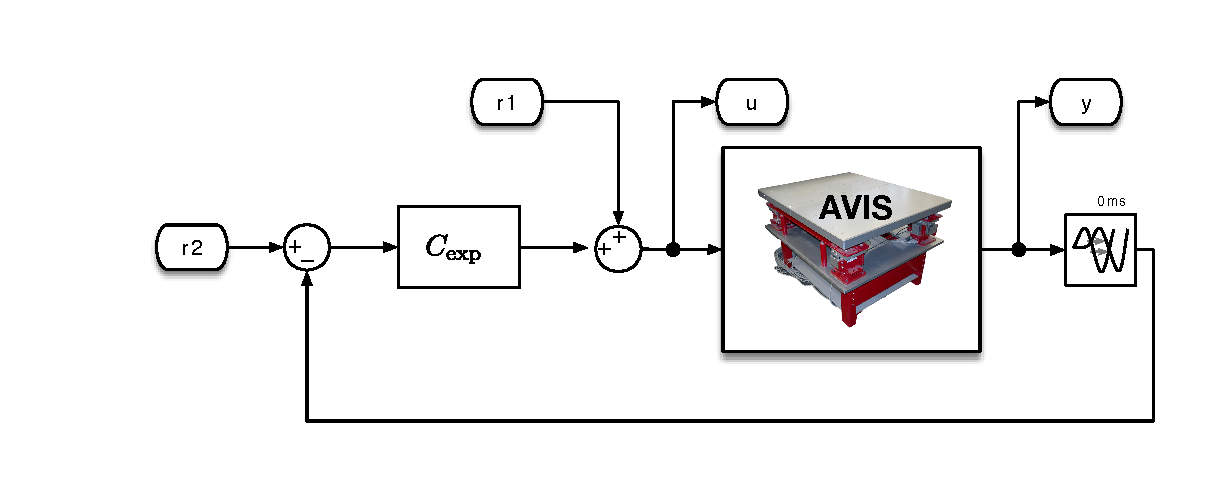
\includegraphics[width=\figurewidth]{\thisDir/figs/simulink-setup.pdf}
  \caption{Simulink model used during the AVIS measurements. All signals are six-dimensional real values.}
  \label{fig:avis:simulink:setup}
\end{figure}

In the top-level model (\figref{fig:avis:simulink:setup}), all signals are six-dimensional and each element corresponds to a mechanical degree-of-freedom of the \gls{AVIS}, i.e. 
\begin{enumerate}
  \item $v_x$: the velocity in $x$ direction (horizontal),
  \item $v_y$: the velocity in $y$ direction (horizontal),
  \item $v_z$: the velocity in $z$ direction (vertical),
  \item $\phi_x$: the angular velocity around the $x$ axis,
  \item $\phi_y$: the angular velocity around the $y$ axis,
  \item $\phi_z$: the angular velocity around the $z$ axis.
\end{enumerate}
The coordinate frame and axes are indicated in \figref{fig:avis:withAxes}.

\begin{figure}
  \centering
  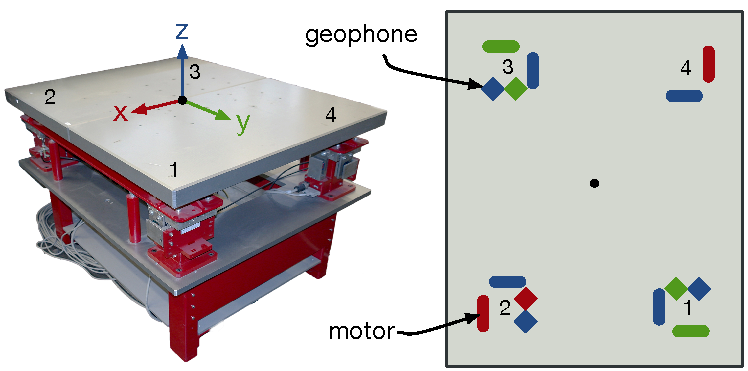
\includegraphics{\thisDir/figs/avis-with-axes.pdf}
  \caption{\glsentrytext{AVIS} with $(x,y,z)$ coordinate frame indicated and bird's eye view of the approximate locations of the actuators and sensors at each of the four corners. For each of the actuators and sensors, the color indicates the principal direction.}
  \label{fig:avis:withAxes}
\end{figure}

In the main text, we have simplified this system to consider only $v_z$, the vertical translation (i.e. the third signal).
For the other directions, the applied signals (\code{r1} and \code{r2}) were set to $0$.
However, inside the feedback loop, all directions are controlled by the experimental controller $\experimental\Controller$.

Specifically, $\experimental\Controller$ is a $6\times6$ transfer function matrix that is implemented as a discrete state-space model.
This controller was constructed by~\citet{Rademakers2005MSc}
 and is given by the state-space matrices below
\begin{align}
  \experimental\Controller & \isdef 
  \begin{cases}
     x[n+1] &= A x[n] + B u_c\\
       y_c    &= C x + D u_c 
  \end{cases}\\
  A       &\approx 828.8 \cdot 10^{-3} \cdot \Identity{6} \\
  B = C &\approx \AvisMatrixDiagonal{93.83}{39.57} \cdot 10^{-3}\\
  D       &= \AvisMatrixDiagonal{4.982}{0.886} \cdot 10^{-3}
\end{align}
with $\Identity{n}$ the $n\times n$ identify matrix.
It can be seen that the controller is diagonal, i.e. the directions are decoupled, and that the dynamics are common among the translational directions and the rotational directions respectively, such that
\begin{equation}
  \experimental\Controller = 
  \AvisMatrixDiagonal{\experimental\Controller_{\mathrm{tran}}}{\experimental\Controller_{\mathrm{rot}}}
\end{equation}
with
\begin{align}
\experimental\Controller_{\mathrm{tran}} &  \approx 
   \frac{4.9821 z + 4.6787}{ z - 0.8282} \cdot 10^{-3} \\
  \experimental\Controller_{\mathrm{rot}} & \approx 
    \frac{0.88595 z + 0.83201}{ z - 0.8282} \cdot 10^{-3}
\end{align}
 as visualized in \figref{fig:avis:bodeplots:controllerAndSensor}.

\begin{figure}[p]
\setlength\figurewidth{0.75\columnwidth}
\setlength\figureheight{0.68\figurewidth}
% This file was created by matlab2tikz.
%
%The latest updates can be retrieved from
%  http://www.mathworks.com/matlabcentral/fileexchange/22022-matlab2tikz-matlab2tikz
%where you can also make suggestions and rate matlab2tikz.
%
\begin{tikzpicture}


\pgfplotsset{amplitudePlot/.append style={%
  height=0.5\figureheight,
  ylabel={Amplitude \axisunit{dB}}}}
\pgfplotsset{phasePlot/.append style={%
  height=0.5\figureheight,
  ylabel={Phase \axisunit{rad}},
  ytick={-3.1416,-1.5708,0,1.5708,3.1416},
  yticklabels={{$-\pi$},$-\pi/2$,$0$,$\pi/2$,$\pi$},
  ymin=-3.142,
  ymax=3.142
  }}
\pgfplotsset{controllerAmpl/.append style={ymin=-80,ymax=-20}}
\pgfplotsset{filterAmpl/.append style={ymin=-20,ymax=20, yticklabel pos=right, ylabel near ticks, ytick={-20,0,20}}}
\pgfplotsset{noXTicks/.append style={xticklabels={}}}
\pgfplotsset{noYTicks/.append style={yticklabels={}}}
\pgfplotsset{noXLabel/.append style={xlabel={}, noXTicks}}
\pgfplotsset{noYLabel/.append style={ylabel={}, noYTicks}}


\begin{groupplot}[%
group style={%
  group name=derivs,
  group size=3 by 2,
  horizontal sep=0.5em,
  vertical sep=1em},
xlabel={Frequency $\omega \axisunit{Hz}$},
scale only axis,
xmode=log,
xmin=0.00016,
xmax=500,
xtick={0.01, 1, 100},
xminorticks=true,
grid=major,
width=0.33\figurewidth]


% ================================================
\nextgroupplot[amplitudePlot, controllerAmpl, noXLabel, title={$\experimental\Controller_{\mathrm{tran}}$}]
\addplot[myDerivs] table[] {\thisDir/data/avis-setup/Ctran-mag.tsv};

% ================================================
\nextgroupplot[amplitudePlot, controllerAmpl, noYLabel, noXLabel, title={$\experimental\Controller_{\mathrm{rot}}$}]
\addplot[myDerivs] table[] {\thisDir/data/avis-setup/Crot-mag.tsv};

% ================================================
\nextgroupplot[amplitudePlot, filterAmpl, noXLabel, title={$F_{\phantom{rot}}$}]
\addplot[myDerivs] table[] {\thisDir/data/avis-setup/sensFilter-mag.tsv};

% ================================================
% ================================================

% ================================================
\nextgroupplot[phasePlot]
\addplot[myDerivs] table[] {\thisDir/data/avis-setup/Ctran-phase.tsv};

% ================================================
\nextgroupplot[phasePlot, noYLabel, noYTicks]
\addplot[myDerivs] table[] {\thisDir/data/avis-setup/Crot-phase.tsv};

% ================================================
\nextgroupplot[phasePlot, noYLabel, noYTicks]
\addplot[myDerivs] table[] {\thisDir/data/avis-setup/sensFilter-phase.tsv};

\end{groupplot}

\end{tikzpicture}%

\caption{Bode plots of the elements of $\experimental\Controller$ and sensor filter $F$ present in the set-up.}
\label{fig:avis:bodeplots:controllerAndSensor}
\end{figure}

For multisine excitations the \code{RepeatingSequence} block was used to load the \code{r2} signal from \MATLAB, for noise excitations, the \code{RandomNumber} block of \Simulink was used instead.
The signals \code{r2}, \code{u} and \code{y} are returned from \Simulink to \MATLAB where further processing of the data is carried out.
This allows to compute the transfer function from \code{r2} to \code{u} and \code{y} respectively, or, the transfer function of the \gls{AVIS} block in the \Simulink model.

\begin{figure}[p]
\setlength\figurewidth{\columnwidth}
  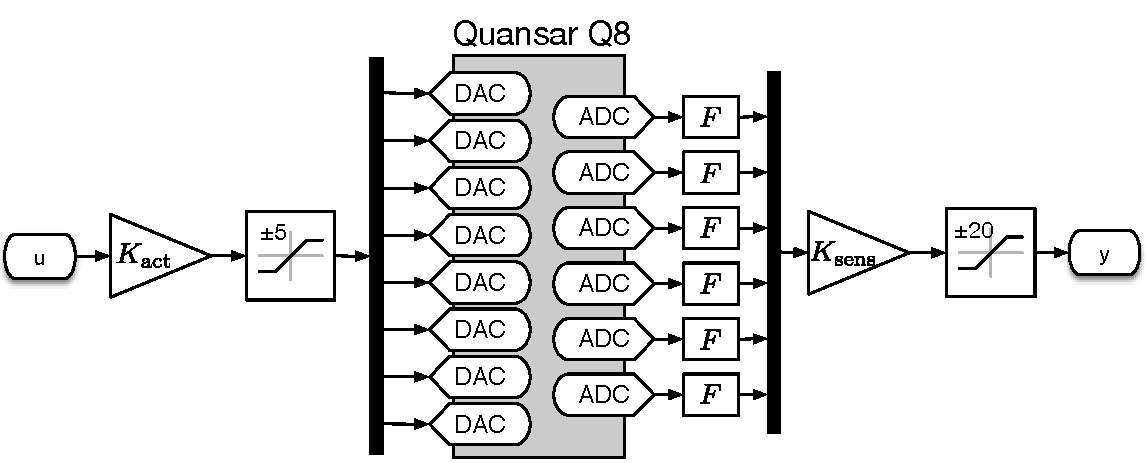
\includegraphics[width=\figurewidth]{\thisDir/figs/simulink-avis.pdf}
  \caption{Simulink model of the AVIS sub-block.}
  \label{fig:avis:simulink:avis}
\end{figure}

The \gls{AVIS} block (\figref{fig:avis:simulink:avis}), conceptually, contains:
\begin{itemize}
  \item static transformations $(K_{\mathrm{act}}, K_{\mathrm{sens}})$, as derived from first principles in~\citep{Rademakers2005MSc}, which translates the sensor and actuator signals to physical velocities at the center of the payload,
  \item logic to communicate with the Quanser Q8 \gls{DAQ} board which is physically connected to the \gls{AVIS}, and
  \item signal conditioning.
\end{itemize}

In \citet[Appendix A.4]{Rademakers2005MSc}, linear static relationships are derived to link the velocities at the center of the payload to the corresponding actuator voltages.
This yields the matrix:
\begin{align}
  K_{\mathrm{act}}    & \approx \begin{bmatrix}
     \deemph{0} &   -0.5 &      \deemph{0} &      \deemph{0} &      \deemph{0} & -0.6485\\
0.0974 & 0.1233 &  -0.25 & -0.6667 & 0.5263 &      \deemph{0}\\
  -0.5 &      \deemph{0} &      \deemph{0} &      \deemph{0} &      \deemph{0} & -0.5119\\
0.0974 & -0.1233 & -0.255 & 0.6667 & 0.5263 &      \deemph{0}\\
     \deemph{0} &    0.5 &      \deemph{0} &      \deemph{0} &      \deemph{0} & -0.6485\\
-0.0974 & -0.1233 &  -0.25 & 0.6667 & -0.5263 &      \deemph{0}\\
   0.5 &      \deemph{0} &      \deemph{0} &      \deemph{0} &      \deemph{0} & -0.5119\\
-0.0974 & 0.1233 &  -0.25 & -0.6667 & -0.5263 &      \deemph{0}\\
\end{bmatrix}
\\
\end{align}
Note that $K_{\mathrm{act}} \in \RR^{8\times6}$ and hence produces signals for the $8$ actuators on the \gls{AVIS}.
These signals are limited to the range $\pm 5\unit{V}$ before they are sent to the \glspl{DAC} on the Q8 \gls{DAQ} board to avoid overdriving the \glspl{DAC}.

The $6$ velocity signals that are digitized by the Q8 \gls{DAQ} are each filtered to transform the voltage induced in the coils of the geophones on the \gls{AVIS} into a velocity using a filter $F$ with transfer function
\begin{equation}
  F(s) \approx \frac{6.51 s^2 + 122 s + 11.3}{6.4 s^2 - 16.6 s - 2.2}

\end{equation}
which is shown in \figref{fig:avis:bodeplots:controllerAndSensor}.
More information regarding this design is given in \citep[Appendix A.3]{Rademakers2005MSc}.
This filter is discretized automatically by \Simulink for the actual implementation.
These velocities are then linked by a linear transformation to the (angular) velocities

The output \code{y} is clipped to $\pm 20$ for easier detection of errors.
However, during normal operation and all the measurements, the signal levels were well within the linear region of this saturation block.

\begin{remark}
It should be noted that while the benchmark paper by \citet{Voorhoeve2015SYSID} deals with the same physical \gls{AVIS}, the experimental data of the benchmark is fundamentally different from the data presented here.
\Citet{Voorhoeve2015SYSID} only consider the `physical' \gls{AVIS} with $8$ inputs and $6$ outputs as indicated by the \code{QuanserQ8} block in \figref{fig:avis:simulink:avis} as the system under test.
The measurements of the benchmark data were carried out in open-loop.
Hence, the experimental controller ($\experimental\Controller_{\mathrm{benchmark}} = 0$),the saturations, the filter $F$ and the static matrices $K$ are different.
Moreover, the sample rate of the benchmark data is much higher ($\fs  = 20 \unit{kHz}$) compared to the data in this work ($\fs = 1\unit{kHz}$) thanks to an upgrade of the real-time computer responsible for acquiring the signals.
\end{remark}


\end{subappendices}
